% !TeX spellcheck = en_US
% !TEX TS-program = pdflatex
% !TEX encoding = IsoLatin

%% Version 4x3 und 16x9  2.2 02.01.2014

%Based on ETH official latex template
%Modified for ASL by Alvaro Estandia (09.02.2015) (ealvaro@student.ethz.ch)

% ==== wrapper class ==========================================================
\documentclass[% wrapper-class ETHpres option inspite of aspectratio for beamer-classe
    fourtothree=true, % true (default) -- 4:3-format, false -- 16:9-format
    DepLogo=true     % true -- use deplogo_13.pdf, false (default) 
                      %         do not use deplogo_13.pdf for footer
    ]{ETHpres}

% ==== misc: you may use or not ===============================================
%\usepackage{graphicx}   % for including figures
%%\graphicspath{{pictures/}}
%\usepackage{tabularx}   % for special table environment (tabularx-table)
%\usepackage{booktabs}   % for table layout
%\usepackage{natbib}     % for bibliography with astron-style
%\bibliographystyle{astron}
%\usepackage{siunitx}    % to use for international units in the real world
%\usepackage[
%    colorlinks=true, linkcolor=white, urlcolor=white, % this is special for this presentation here to get the toc in white
%    hypertexnames=false,% for correct links (duplicate-error solution)
%	setpagesize=false,  % necessary in order to not change text-/paperformat for the document
%	pdfborder={0 0 0},  % removes border around links
%	pdfpagemode=FullScreen,% open pdf in full screen mode
%    pdfstartview=Fit    % fit page to pdf viewer
%]{hyperref}% all links stay black and are thus invisible

%----- My Packages
\titlespacing{\section}{0pt}{-25pt}{0pt}
\titlespacing{\subsubsection}{0pt}{5pt}{0pt}

\usepackage{amsmath}
\usepackage{caption}
\usepackage{comment}
\usepackage[makeroom]{cancel}


\setitemize{noitemsep,topsep=0pt,parsep=0pt,partopsep=0pt}

%\usepackage{soul} Highligh text \hl{Some Text}
\usepackage{media9} %Add videos

%ASL Packages
\usepackage[numbers]{natbib}
\usepackage{enumitem}
\usepackage{units}

\usepackage{isomath}
\renewcommand{\vec}{\vectorsym}
\newcommand{\mat}{\matrixsym}

% URL citing
\usepackage{url}

% SI units
\usepackage{siunitx}

% block diagram with tikz
\usepackage{tikz}
\usepackage{tikzscale}	% includegraphics .tikz
\usetikzlibrary{calc}

% Matrix alligned subfigures
\usepackage[lofdepth,lotdepth]{subfig}

%clock time
\usepackage{datetime}

% matlab2tikz pictures
\usepackage{pgfplots}
% externalize tikz library (faster compilation)
%\usetikzlibrary{external} \tikzexternalize[prefix=tikz/]

% source code
\usepackage{listings}
\lstdefinelanguage{myMatlab}{
	language = Matlab,%    
	basicstyle=\small,%
    breaklines=true,%
    morekeywords={matlab2tikz},
    keywordstyle=\color{blue},%
    morekeywords=[2]{1}, keywordstyle=[2]{\color{black}},
    identifierstyle=\color{black},%
    stringstyle=\color{mylilas},
    commentstyle=\color{mygreen},%
    showstringspaces=false,%without this there will be a symbol in the places where there is a space
    numbers=left,%
    numberstyle={\tiny \color{black}},% size of the numbers
    numbersep=9pt, % this defines how far the numbers are from the text
    emph=[1]{for,end,break},emphstyle=[1]\color{red}, %some words to emphasise
    %emph=[2]{word1,word2}, emphstyle=[2]{style},    
    frame=single,%
}
\lstdefinelanguage{myCVXGEN}{
	language=sh,%
	basicstyle=\small,%
    classoffset=0,%
    morekeywords={dimensions,end,parameters,variables,minimize,subject,to},
    keywordstyle=\color{blue},%
    classoffset=1,%
    morekeywords={diagonal,psd},%
    keywordstyle=\color{darkblue}\it,%
    classoffset=0,%
    moredelim=[s][\color{darkgreen}]{[}{]},%
    moredelim=[s][\color{orange}]{(n}{)},%
    commentstyle=\color{gray},%
    numbers=left,%
    numberstyle={\tiny \color{black}},% size of the numbers
    numbersep=9pt, % this defines how far the numbers are from the text
    frame=single,%
    literate={\ t=0..N}{{\textbf{\textcolor{darkgreen}{\ t=0..N}}}}{7} {\ t=1..N+1}{{\textbf{\textcolor{darkgreen}{\ t=1..N+1}}}}{9} {\ t=0..N-1}{{\textbf{\textcolor{darkgreen}{\ t=0..N-1}}}}{9} {2}{{\textcolor{mypurple}{2}}}{1} {3}{{\textcolor{mypurple}{3}}}{1} {10}{{\textcolor{mypurple}{10}}}{2} {20}{{\textcolor{mypurple}{20}}}{2} {40}{{\textcolor{mypurple}{40}}}{2} {==}{{\textcolor{darkblue}{$==$}}}{2} {<=}{{\textcolor{darkblue}{$<=$}}}{2} {>=}{{\textcolor{darkblue}{$>=$}}}{2} {\ =\ }{{\textcolor{darkgreen}{\ $=$\ }}}{3},%
    moredelim=[s][\color{mypurple}]{\{1,1\ 1,2}{\}},%
    moredelim=[s][\color{mypurple}]{\{5,1}{\}},%
    moredelim=[s][\color{mypurple}]{\{1,1\ 2,1}{\}},%
}

% remarks, theorems etc.
\usepackage{amsthm}
\theoremstyle{remark}
\newtheorem{remark}{Remark}

% larger symbols in math environment for block matrix
\usepackage{relsize}

% algorithms (pseudocode)
\usepackage{algorithm}
\usepackage{algpseudocode}

% cvxcode
\usepackage{upquote}
\definecolor{pdefvalue}{rgb}{0.467,0.000,0.533}
\newcommand{\pdefvalue}[1]{\textcolor{pdefvalue}{#1}}
\definecolor{pdefidentifier}{rgb}{0.000,0.000,0.000}
\newcommand{\pdefidentifier}[1]{\textcolor{pdefidentifier}{#1}}
\definecolor{pdefcomment}{rgb}{0.502,0.502,0.502}
\newcommand{\pdefcomment}[1]{\textcolor{pdefcomment}{#1}}
\definecolor{pdefblock}{rgb}{0.267,0.533,0.867}
\newcommand{\pdefblock}[1]{\textcolor{pdefblock}{#1}}
\definecolor{pdeferror}{rgb}{0.667,0.000,0.000}
\newcommand{\pdeferror}[1]{\textcolor{pdeferror}{#1}}
\definecolor{pdefequals}{rgb}{0.000,0.490,0.000}
\newcommand{\pdefequals}[1]{\textcolor{pdefequals}{#1}}
\definecolor{pdefdim}{rgb}{0.973,0.502,0.090}
\newcommand{\pdefdim}[1]{\textcolor{pdefdim}{#1}}
\definecolor{pdefattr}{rgb}{0.000,0.000,0.467}
\newcommand{\pdefattr}[1]{\textcolor{pdefattr}{#1}}
\definecolor{pdefconstr}{rgb}{0.000,0.000,0.000}
\newcommand{\pdefconstr}[1]{\textcolor{pdefconstr}{#1}}
\definecolor{pdefobjv}{rgb}{0.000,0.000,0.000}
\newcommand{\pdefobjv}[1]{\textcolor{pdefobjv}{#1}}
\definecolor{pdefconstrsign}{rgb}{0.000,0.000,0.800}
\newcommand{\pdefconstrsign}[1]{\textcolor{pdefconstrsign}{#1}}
\definecolor{pdefrange}{rgb}{0.333,0.467,0.200}
\newcommand{\pdefrange}[1]{\textcolor{pdefrange}{#1}}
\definecolor{pdefindex}{rgb}{0.333,0.467,0.200}
\newcommand{\pdefindex}[1]{\textcolor{pdefindex}{#1}}
\definecolor{pdefbrackets}{rgb}{0.333,0.467,0.200}
\newcommand{\pdefbrackets}[1]{\textcolor{pdefbrackets}{#1}}
\definecolor{pdefsemicolon}{rgb}{0.133,0.400,0.800}
\newcommand{\pdefsemicolon}[1]{\textcolor{pdefsemicolon}{#1}}
\definecolor{pdeffunction}{rgb}{0.000,0.333,0.667}
\newcommand{\pdeffunction}[1]{\textcolor{pdeffunction}{#1}}
\definecolor{pdefdenom}{rgb}{0.000,0.333,0.667}
\newcommand{\pdefdenom}[1]{\textcolor{pdefdenom}{#1}}
\definecolor{pdefsparseindices}{rgb}{0.667,0.000,0.533}
\newcommand{\pdefsparseindices}[1]{\textcolor{pdefsparseindices}{#1}}


% colors
\definecolor{mygreen}{RGB}{28,172,0} % color values Red, Green, Blue
\definecolor{mylilas}{RGB}{170,55,241}
\definecolor{mypurple}{RGB}{128,0,128}
\definecolor{myorchid}{RGB}{186,85,211}

% find inkscape pdfs
\graphicspath{{images/}}


% ==== language ================================================================
\usepackage[latin1]{inputenc}
%\usepackage[utf8]{inputenc}
% English
\usepackage[english]{babel}
\AtBeginDocument{\renewcaptionname{english}{\contentsname}{ }}% toc-name
%% Deutsch
%\usepackage[ngerman]{babel}
%\AtBeginDocument{\renewcaptionname{ngerman}{\contentsname}{ }}% toc-name

% ==== choose the basic color for your presentation ===========================
% colorbar-color
\colorlet{firstcolor}{ETHc} % see pages 2  and 3 of this sample presentation
% bachground color titlepage
\colorlet{secondcolor}{ETHc} % see pages 2  and 3 of this sample presentation

% === fill in first information for the presentation ==========================
\newcommand*{\ETHtitle}{Incorporating Aerodynamic Effects into Model Based Con\-trol for Multirotors}
\newcommand*{\ETHauthor}{Rik B\"ahnemann}
\newcommand*{\ETHdate}{30.06.2015}


\begin{document}
% =========== begin of titlepage ============
\ETHtitelbild\textcolor{white}{\large\textbf{\ETHtitle}}\\~\newline\hspace{6mm}\normalsize%
%%
% ==== start here with the text on the titlepage
\textcolor{white}{
\textbf{\ETHauthor}\\ \\
Semester Project\\
Supervised by Markus Achtelik, Michael Burri, Mina Kamel}\\
%%

\clearpage
% =========== begin of the standard page ============

\ETHslide
\section*{Motivation}
\vspace*{\fill}

%\addcontentsline{toc}{section}{Motivation}
\begin{minipage}{0.5\textwidth}
	\begin{itemize}
		\item[\ETHitem] Multirotors
		\item[\ETHitem] autonomous flight \\ position control
		\item[\ETHitem] Wind
\end{itemize}
\end{minipage}
\begin{minipage}{0.49\textwidth}
	\centering
	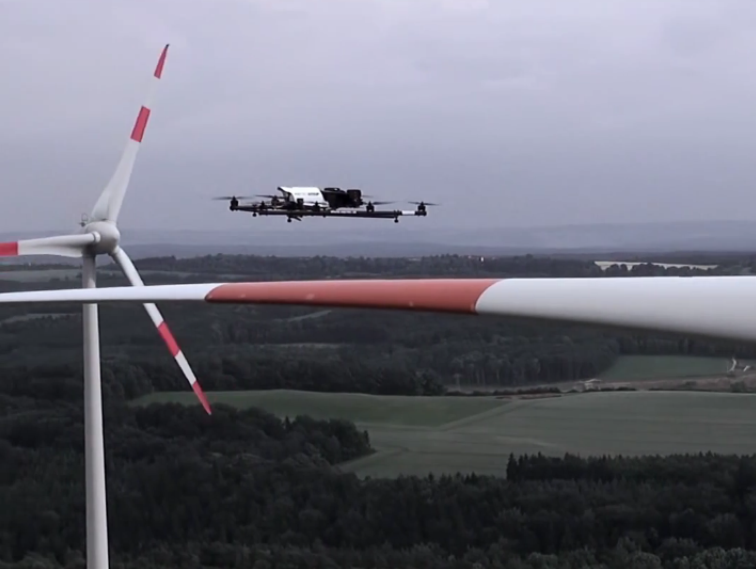
\includegraphics[width=1\textwidth]{images/mav_wind_turbine.png}\\
	\tiny{AscTec Falcon 8 at wind turbine inspection, \cite{www:asctecinspect}} 
\end{minipage}

\vspace*{\fill}
\clearpage

\ETHslide
\section*{Overview}
\tableofcontents
\clearpage

\addcontentsline{toc}{section}{Modelling}
\ETHslide
\section*{Equations of Motion}
%\addcontentsline{toc}{section}{Modelling}
\vspace*{\fill}

%\centering
%\def\svgwidth{0.45\textwidth}
%\tiny{
%\input{images/hexa.pdf_tex}
%}
%
%\normalsize{	
%\begin{align}
%m \cdot \mathbf{a} &= \rotWB \sum_{i=1}^n \underbrace{\left(\mathbf{F}_{T,i} + \mathbf{F}_{D,i} \right)}_{=:\mathbf{F}_i} + \mathbf{F}_G \\
%\mathbf{J} \cdot  \mathbf{\dot{\boldsymbol{\omega}}} + \boldsymbol{\omega} \times \mathbf{J} \cdot \boldsymbol{\omega} &= \sum_{i=1}^n \left( \mathbf{M}_{R,i}+ \mathbf{M}_{D,i} + \mathbf{F}_i \times \mathbf{l}_i \right)
%\end{align}
%}

\begin{minipage}{0.5\textwidth}
	\centering
    \def\svgwidth{1\textwidth}
    \tiny{
	\input{images/hexa.pdf_tex}}
\end{minipage}
\begin{minipage}{0.49\textwidth}
\footnotesize{
\begin{align}
m \cdot \mathbf{a} &= \rotWB \sum_{i=1}^n \underbrace{\left(\mathbf{F}_{T,i} + \mathbf{F}_{D,i} \right)}_{=:\mathbf{F}_i} + \mathbf{F}_G \nonumber \\
\mathbf{J} \cdot  \mathbf{\dot{\boldsymbol{\omega}}} + \boldsymbol{\omega} \times \mathbf{J} \cdot \boldsymbol{\omega} &= \sum_{i=1}^n \left( \mathbf{M}_{R,i}+ \mathbf{M}_{D,i} + \mathbf{F}_i \times \mathbf{l}_i \right) \nonumber
\end{align}}
\end{minipage}

\vspace*{\fill}
\clearpage
\ETHslide
\section*{Wind Drag}
%\addcontentsline{toc}{section}{Wind Drag}
\vspace*{\fill}


\begin{minipage}{0.5\textwidth}
\begin{itemize}
	\item[\ETHitem] Air speed
	\begin{itemize}
	\item[\ETHitem] $\boldsymbol{\nu} = \mathbf{v}-\mathbf{w}  $
	\end{itemize}
	\item[\ETHitem] Area drag \cite{Schiano2014}
	\begin{itemize}
	\item[\ETHitem] $\mathbf{F}_A = -\frac{1}{2} C_A \rho \norm{\boldsymbol{\nu}}_2 \boldsymbol{\nu}  $
	\end{itemize}
	\item[\ETHitem] Rotor drag
	\begin{itemize}
	\item[\ETHitem] $\mathbf{F}_D =  -\sum_{i=1}^n \omega_i \cdot  C_D \cdot \boldsymbol{\nu}^\perp$
	\end{itemize}
\end{itemize}
\end{minipage}
\begin{minipage}{0.49\textwidth}
	\centering
	\tiny{
	% This file was created by matlab2tikz.
% Minimal pgfplots version: 1.3
%
%The latest updates can be retrieved from
%  http://www.mathworks.com/matlabcentral/fileexchange/22022-matlab2tikz
%where you can also make suggestions and rate matlab2tikz.
%
\definecolor{mycolor1}{rgb}{0.00000,0.44700,0.74100}%
\definecolor{mycolor2}{rgb}{0.85000,0.32500,0.09800}%
%
\begin{tikzpicture}

\begin{axis}[%
width=0.95092\figurewidth,
height=\figureheight,
at={(0\figurewidth,0\figureheight)},
scale only axis,
xmin=0,
xmax=20,
xlabel={Wind velocity $[\si{\metre\per\second}]$},
ymin=0,
ymax=6,
ytick={0, 1, 2, 3, 4, 5},
ylabel={Drag force [\si{\newton}]},
legend style={legend cell align=left,align=left,draw=white!15!black}
]
\addplot [color=mycolor1,solid]
  table[row sep=crcr]{%
0	0\\
0.02002002002002	4.90981471962453e-06\\
0.04004004004004	1.96392588784981e-05\\
0.0600600600600601	4.41883324766208e-05\\
0.0800800800800801	7.85570355139925e-05\\
0.1001001001001	0.000122745367990613\\
0.12012012012012	0.000176753329906483\\
0.14014014014014	0.000240580921261602\\
0.16016016016016	0.00031422814205597\\
0.18018018018018	0.000397694992289587\\
0.2002002002002	0.000490981471962453\\
0.22022022022022	0.000594087581074568\\
0.24024024024024	0.000707013319625932\\
0.26026026026026	0.000829758687616546\\
0.28028028028028	0.000962323685046408\\
0.3003003003003	0.00110470831191552\\
0.32032032032032	0.00125691256822388\\
0.34034034034034	0.00141893645397149\\
0.36036036036036	0.00159077996915835\\
0.38038038038038	0.00177244311378446\\
0.4004004004004	0.00196392588784981\\
0.42042042042042	0.00216522829135442\\
0.44044044044044	0.00237635032429827\\
0.46046046046046	0.00259729198668138\\
0.48048048048048	0.00282805327850373\\
0.500500500500501	0.00306863419976533\\
0.520520520520521	0.00331903475046618\\
0.540540540540541	0.00357925493060628\\
0.560560560560561	0.00384929474018563\\
0.580580580580581	0.00412915417920423\\
0.600600600600601	0.00441883324766208\\
0.620620620620621	0.00471833194555917\\
0.640640640640641	0.00502765027289552\\
0.660660660660661	0.00534678822967111\\
0.680680680680681	0.00567574581588596\\
0.700700700700701	0.00601452303154005\\
0.720720720720721	0.00636311987663339\\
0.740740740740741	0.00672153635116598\\
0.760760760760761	0.00708977245513782\\
0.780780780780781	0.00746782818854891\\
0.800800800800801	0.00785570355139925\\
0.820820820820821	0.00825339854368884\\
0.840840840840841	0.00866091316541767\\
0.860860860860861	0.00907824741658575\\
0.880880880880881	0.00950540129719309\\
0.900900900900901	0.00994237480723967\\
0.920920920920921	0.0103891679467255\\
0.940940940940941	0.0108457807156506\\
0.960960960960961	0.0113122131140149\\
0.980980980980981	0.0117884651418185\\
1.001001001001	0.0122745367990613\\
1.02102102102102	0.0127704280857434\\
1.04104104104104	0.0132761390018647\\
1.06106106106106	0.0137916695474253\\
1.08108108108108	0.0143170197224251\\
1.1011011011011	0.0148521895268642\\
1.12112112112112	0.0153971789607425\\
1.14114114114114	0.0159519880240601\\
1.16116116116116	0.0165166167168169\\
1.18118118118118	0.017091065039013\\
1.2012012012012	0.0176753329906483\\
1.22122122122122	0.0182694205717229\\
1.24124124124124	0.0188733277822367\\
1.26126126126126	0.0194870546221898\\
1.28128128128128	0.0201106010915821\\
1.3013013013013	0.0207439671904136\\
1.32132132132132	0.0213871529186845\\
1.34134134134134	0.0220401582763945\\
1.36136136136136	0.0227029832635438\\
1.38138138138138	0.0233756278801324\\
1.4014014014014	0.0240580921261602\\
1.42142142142142	0.0247503760016273\\
1.44144144144144	0.0254524795065336\\
1.46146146146146	0.0261644026408791\\
1.48148148148148	0.0268861454046639\\
1.5015015015015	0.027617707797888\\
1.52152152152152	0.0283590898205513\\
1.54154154154154	0.0291102914726538\\
1.56156156156156	0.0298713127541956\\
1.58158158158158	0.0306421536651767\\
1.6016016016016	0.031422814205597\\
1.62162162162162	0.0322132943754565\\
1.64164164164164	0.0330135941747553\\
1.66166166166166	0.0338237136034934\\
1.68168168168168	0.0346436526616707\\
1.7017017017017	0.0354734113492872\\
1.72172172172172	0.036312989666343\\
1.74174174174174	0.0371623876128381\\
1.76176176176176	0.0380216051887724\\
1.78178178178178	0.0388906423941459\\
1.8018018018018	0.0397694992289587\\
1.82182182182182	0.0406581756932107\\
1.84184184184184	0.041556671786902\\
1.86186186186186	0.0424649875100326\\
1.88188188188188	0.0433831228626023\\
1.9019019019019	0.0443110778446114\\
1.92192192192192	0.0452488524560597\\
1.94194194194194	0.0461964466969472\\
1.96196196196196	0.047153860567274\\
1.98198198198198	0.04812109406704\\
2.002002002002	0.0490981471962453\\
2.02202202202202	0.0500850199548898\\
2.04204204204204	0.0510817123429736\\
2.06206206206206	0.0520882243604966\\
2.08208208208208	0.0531045560074589\\
2.1021021021021	0.0541307072838604\\
2.12212212212212	0.0551666781897012\\
2.14214214214214	0.0562124687249812\\
2.16216216216216	0.0572680788897005\\
2.18218218218218	0.058333508683859\\
2.2022022022022	0.0594087581074568\\
2.22222222222222	0.0604938271604938\\
2.24224224224224	0.0615887158429701\\
2.26226226226226	0.0626934241548856\\
2.28228228228228	0.0638079520962404\\
2.3023023023023	0.0649322996670344\\
2.32232232232232	0.0660664668672677\\
2.34234234234234	0.0672104536969402\\
2.36236236236236	0.068364260156052\\
2.38238238238238	0.069527886244603\\
2.4024024024024	0.0707013319625932\\
2.42242242242242	0.0718845973100227\\
2.44244244244244	0.0730776822868915\\
2.46246246246246	0.0742805868931995\\
2.48248248248248	0.0754933111289468\\
2.5025025025025	0.0767158549941333\\
2.52252252252252	0.077948218488759\\
2.54254254254254	0.079190401612824\\
2.56256256256256	0.0804424043663283\\
2.58258258258258	0.0817042267492718\\
2.6026026026026	0.0829758687616546\\
2.62262262262262	0.0842573304034765\\
2.64264264264264	0.0855486116747378\\
2.66266266266266	0.0868497125754383\\
2.68268268268268	0.088160633105578\\
2.7027027027027	0.089481373265157\\
2.72272272272272	0.0908119330541753\\
2.74274274274274	0.0921523124726328\\
2.76276276276276	0.0935025115205295\\
2.78278278278278	0.0948625301978655\\
2.8028028028028	0.0962323685046408\\
2.82282282282282	0.0976120264408553\\
2.84284284284284	0.099001504006509\\
2.86286286286286	0.100400801201602\\
2.88288288288288	0.101809918026134\\
2.9029029029029	0.103228854480106\\
2.92292292292292	0.104657610563516\\
2.94294294294294	0.106096186276366\\
2.96296296296296	0.107544581618656\\
2.98298298298298	0.109002796590384\\
3.003003003003	0.110470831191552\\
3.02302302302302	0.111948685422159\\
3.04304304304304	0.113436359282205\\
3.06306306306306	0.114933852771691\\
3.08308308308308	0.116441165890615\\
3.1031031031031	0.117958298638979\\
3.12312312312312	0.119485251016783\\
3.14314314314314	0.121022023024025\\
3.16316316316316	0.122568614660707\\
3.18318318318318	0.124125025926828\\
3.2032032032032	0.125691256822388\\
3.22322322322322	0.127267307347387\\
3.24324324324324	0.128853177501826\\
3.26326326326326	0.130448867285704\\
3.28328328328328	0.132054376699021\\
3.3033033033033	0.133669705741778\\
3.32332332332332	0.135294854413974\\
3.34334334334334	0.136929822715609\\
3.36336336336336	0.138574610646683\\
3.38338338338338	0.140229218207196\\
3.4034034034034	0.141893645397149\\
3.42342342342342	0.143567892216541\\
3.44344344344344	0.145251958665372\\
3.46346346346346	0.146945844743643\\
3.48348348348348	0.148649550451352\\
3.5035035035035	0.150363075788501\\
3.52352352352352	0.152086420755089\\
3.54354354354354	0.153819585351117\\
3.56356356356356	0.155562569576584\\
3.58358358358358	0.15731537343149\\
3.6036036036036	0.159077996915835\\
3.62362362362362	0.160850440029619\\
3.64364364364364	0.162632702772843\\
3.66366366366366	0.164424785145506\\
3.68368368368368	0.166226687147608\\
3.7037037037037	0.16803840877915\\
3.72372372372372	0.16985995004013\\
3.74374374374374	0.17169131093055\\
3.76376376376376	0.173532491450409\\
3.78378378378378	0.175383491599708\\
3.8038038038038	0.177244311378446\\
3.82382382382382	0.179114950786622\\
3.84384384384384	0.180995409824239\\
3.86386386386386	0.182885688491294\\
3.88388388388388	0.184785786787789\\
3.9039039039039	0.186695704713723\\
3.92392392392392	0.188615442269096\\
3.94394394394394	0.190544999453908\\
3.96396396396396	0.19248437626816\\
3.98398398398398	0.194433572711851\\
4.004004004004	0.196392588784981\\
4.02402402402402	0.198361424487551\\
4.04404404404404	0.200340079819559\\
4.06406406406406	0.202328554781007\\
4.08408408408408	0.204326849371894\\
4.1041041041041	0.206334963592221\\
4.12412412412412	0.208352897441987\\
4.14414414414414	0.210380650921192\\
4.16416416416416	0.212418224029836\\
4.18418418418418	0.214465616767919\\
4.2042042042042	0.216522829135442\\
4.22422422422422	0.218589861132404\\
4.24424424424424	0.220666712758805\\
4.26426426426426	0.222753384014645\\
4.28428428428428	0.224849874899925\\
4.3043043043043	0.226956185414644\\
4.32432432432432	0.229072315558802\\
4.34434434434434	0.2311982653324\\
4.36436436436436	0.233334034735436\\
4.38438438438438	0.235479623767912\\
4.4044044044044	0.237635032429827\\
4.42442442442442	0.239800260721182\\
4.44444444444444	0.241975308641975\\
4.46446446446446	0.244160176192208\\
4.48448448448448	0.24635486337188\\
4.5045045045045	0.248559370180992\\
4.52452452452452	0.250773696619542\\
4.54454454454454	0.252997842687532\\
4.56456456456456	0.255231808384962\\
4.58458458458458	0.25747559371183\\
4.6046046046046	0.259729198668138\\
4.62462462462462	0.261992623253885\\
4.64464464464464	0.264265867469071\\
4.66466466466466	0.266548931313696\\
4.68468468468468	0.268841814787761\\
4.7047047047047	0.271144517891265\\
4.72472472472472	0.273457040624208\\
4.74474474474474	0.27577938298659\\
4.76476476476476	0.278111544978412\\
4.78478478478478	0.280453526599673\\
4.8048048048048	0.282805327850373\\
4.82482482482482	0.285166948730512\\
4.84484484484484	0.287538389240091\\
4.86486486486486	0.289919649379109\\
4.88488488488488	0.292310729147566\\
4.9049049049049	0.294711628545462\\
4.92492492492492	0.297122347572798\\
4.94494494494494	0.299542886229573\\
4.96496496496496	0.301973244515787\\
4.98498498498498	0.30441342243144\\
5.00500500500501	0.306863419976533\\
5.02502502502503	0.309323237151065\\
5.04504504504505	0.311792873955036\\
5.06506506506507	0.314272330388447\\
5.08508508508509	0.316761606451296\\
5.10510510510511	0.319260702143585\\
5.12512512512513	0.321769617465313\\
5.14514514514515	0.324288352416481\\
5.16516516516517	0.326816906997087\\
5.18518518518519	0.329355281207133\\
5.20520520520521	0.331903475046618\\
5.22522522522523	0.334461488515543\\
5.24524524524525	0.337029321613906\\
5.26526526526527	0.339606974341709\\
5.28528528528529	0.342194446698951\\
5.30530530530531	0.344791738685633\\
5.32532532532533	0.347398850301753\\
5.34534534534535	0.350015781547313\\
5.36536536536537	0.352642532422312\\
5.38538538538539	0.355279102926751\\
5.40540540540541	0.357925493060628\\
5.42542542542543	0.360581702823945\\
5.44544544544545	0.363247732216701\\
5.46546546546547	0.365923581238897\\
5.48548548548549	0.368609249890531\\
5.50550550550551	0.371304738171605\\
5.52552552552553	0.374010046082118\\
5.54554554554555	0.37672517362207\\
5.56556556556557	0.379450120791462\\
5.58558558558559	0.382184887590293\\
5.60560560560561	0.384929474018563\\
5.62562562562563	0.387683880076272\\
5.64564564564565	0.390448105763421\\
5.66566566566567	0.393222151080009\\
5.68568568568569	0.396006016026036\\
5.70570570570571	0.398799700601502\\
5.72572572572573	0.401603204806408\\
5.74574574574575	0.404416528640753\\
5.76576576576577	0.407239672104537\\
5.78578578578579	0.41007263519776\\
5.80580580580581	0.412915417920423\\
5.82582582582583	0.415768020272525\\
5.84584584584585	0.418630442254066\\
5.86586586586587	0.421502683865046\\
5.88588588588589	0.424384745105466\\
5.90590590590591	0.427276625975325\\
5.92592592592593	0.430178326474623\\
5.94594594594595	0.43308984660336\\
5.96596596596597	0.436011186361537\\
5.98598598598599	0.438942345749153\\
6.00600600600601	0.441883324766208\\
6.02602602602603	0.444834123412702\\
6.04604604604605	0.447794741688636\\
6.06606606606607	0.450765179594008\\
6.08608608608609	0.45374543712882\\
6.10610610610611	0.456735514293072\\
6.12612612612613	0.459735411086762\\
6.14614614614615	0.462745127509892\\
6.16616616616617	0.465764663562461\\
6.18618618618619	0.46879401924447\\
6.20620620620621	0.471833194555917\\
6.22622622622623	0.474882189496804\\
6.24624624624625	0.47794100406713\\
6.26626626626627	0.481009638266896\\
6.28628628628629	0.4840880920961\\
6.30630630630631	0.487176365554744\\
6.32632632632633	0.490274458642827\\
6.34634634634635	0.493382371360349\\
6.36636636636637	0.496500103707311\\
6.38638638638639	0.499627655683712\\
6.40640640640641	0.502765027289552\\
6.42642642642643	0.505912218524831\\
6.44644644644645	0.50906922938955\\
6.46646646646647	0.512236059883708\\
6.48648648648649	0.515412710007305\\
6.50650650650651	0.518599179760341\\
6.52652652652653	0.521795469142816\\
6.54654654654655	0.525001578154731\\
6.56656656656657	0.528217506796085\\
6.58658658658659	0.531443255066879\\
6.60660660660661	0.534678822967111\\
6.62662662662663	0.537924210496783\\
6.64664664664665	0.541179417655894\\
6.66666666666667	0.544444444444445\\
6.68668668668669	0.547719290862434\\
6.70670670670671	0.551003956909863\\
6.72672672672673	0.554298442586731\\
6.74674674674675	0.557602747893038\\
6.76676676676677	0.560916872828785\\
6.78678678678679	0.564240817393971\\
6.80680680680681	0.567574581588596\\
6.82682682682683	0.57091816541266\\
6.84684684684685	0.574271568866163\\
6.86686686686687	0.577634791949106\\
6.88688688688689	0.581007834661488\\
6.90690690690691	0.58439069700331\\
6.92692692692693	0.58778337897457\\
6.94694694694695	0.59118588057527\\
6.96696696696697	0.594598201805409\\
6.98698698698699	0.598020342664987\\
7.00700700700701	0.601452303154005\\
7.02702702702703	0.604894083272462\\
7.04704704704705	0.608345683020358\\
7.06706706706707	0.611807102397693\\
7.08708708708709	0.615278341404468\\
7.10710710710711	0.618759400040681\\
7.12712712712713	0.622250278306334\\
7.14714714714715	0.625750976201427\\
7.16716716716717	0.629261493725958\\
7.18718718718719	0.632781830879929\\
7.20720720720721	0.636311987663339\\
7.22722722722723	0.639851964076188\\
7.24724724724725	0.643401760118477\\
7.26726726726727	0.646961375790205\\
7.28728728728729	0.650530811091372\\
7.30730730730731	0.654110066021978\\
7.32732732732733	0.657699140582024\\
7.34734734734735	0.661298034771508\\
7.36736736736737	0.664906748590432\\
7.38738738738739	0.668525282038796\\
7.40740740740741	0.672153635116598\\
7.42742742742743	0.67579180782384\\
7.44744744744745	0.679439800160521\\
7.46746746746747	0.683097612126641\\
7.48748748748749	0.686765243722201\\
7.50750750750751	0.690442694947199\\
7.52752752752753	0.694129965801638\\
7.54754754754755	0.697827056285515\\
7.56756756756757	0.701533966398831\\
7.58758758758759	0.705250696141587\\
7.60760760760761	0.708977245513782\\
7.62762762762763	0.712713614515416\\
7.64764764764765	0.71645980314649\\
7.66766766766767	0.720215811407003\\
7.68768768768769	0.723981639296955\\
7.70770770770771	0.727757286816346\\
7.72772772772773	0.731542753965176\\
7.74774774774775	0.735338040743446\\
7.76776776776777	0.739143147151155\\
7.78778778778779	0.742958073188303\\
7.80780780780781	0.746782818854891\\
7.82782782782783	0.750617384150918\\
7.84784784784785	0.754461769076384\\
7.86786786786787	0.758315973631289\\
7.88788788788789	0.762179997815634\\
7.90790790790791	0.766053841629417\\
7.92792792792793	0.76993750507264\\
7.94794794794795	0.773830988145302\\
7.96796796796797	0.777734290847404\\
7.98798798798799	0.781647413178945\\
8.00800800800801	0.785570355139925\\
8.02802802802803	0.789503116730344\\
8.04804804804805	0.793445697950203\\
8.06806806806807	0.7973980987995\\
8.08808808808809	0.801360319278237\\
8.10810810810811	0.805332359386414\\
8.12812812812813	0.809314219124029\\
8.14814814814815	0.813305898491084\\
8.16816816816817	0.817307397487578\\
8.18818818818819	0.821318716113511\\
8.20820820820821	0.825339854368884\\
8.22822822822823	0.829370812253695\\
8.24824824824825	0.833411589767946\\
8.26826826826827	0.837462186911636\\
8.28828828828829	0.841522603684766\\
8.30830830830831	0.845592840087335\\
8.32832832832833	0.849672896119343\\
8.34834834834835	0.85376277178079\\
8.36836836836837	0.857862467071676\\
8.38838838838839	0.861971981992002\\
8.40840840840841	0.866091316541767\\
8.42842842842843	0.870220470720971\\
8.44844844844845	0.874359444529615\\
8.46846846846847	0.878508237967698\\
8.48848848848849	0.88266685103522\\
8.50850850850851	0.886835283732181\\
8.52852852852853	0.891013536058581\\
8.54854854854855	0.895201608014421\\
8.56856856856857	0.8993994995997\\
8.58858858858859	0.903607210814418\\
8.60860860860861	0.907824741658576\\
8.62862862862863	0.912052092132172\\
8.64864864864865	0.916289262235208\\
8.66866866866867	0.920536251967683\\
8.68868868868869	0.924793061329598\\
8.70870870870871	0.929059690320952\\
8.72872872872873	0.933336138941745\\
8.74874874874875	0.937622407191977\\
8.76876876876877	0.941918495071648\\
8.78878878878879	0.946224402580759\\
8.80880880880881	0.950540129719309\\
8.82882882882883	0.954865676487298\\
8.84884884884885	0.959201042884727\\
8.86886886886887	0.963546228911594\\
8.88888888888889	0.967901234567901\\
8.90890890890891	0.972266059853648\\
8.92892892892893	0.976640704768833\\
8.94894894894895	0.981025169313458\\
8.96896896896897	0.985419453487522\\
8.98898898898899	0.989823557291025\\
9.00900900900901	0.994237480723967\\
9.02902902902903	0.998661223786349\\
9.04904904904905	1.00309478647817\\
9.06906906906907	1.00753816879943\\
9.08908908908909	1.01199137075013\\
9.10910910910911	1.01645439233027\\
9.12912912912913	1.02092723353985\\
9.14914914914915	1.02540989437886\\
9.16916916916917	1.02990237484732\\
9.18918918918919	1.03440467494522\\
9.20920920920921	1.03891679467255\\
9.22922922922923	1.04343873402932\\
9.24924924924925	1.04797049301554\\
9.26926926926927	1.05251207163119\\
9.28928928928929	1.05706346987628\\
9.30930930930931	1.06162468775081\\
9.32932932932933	1.06619572525478\\
9.34934934934935	1.07077658238819\\
9.36936936936937	1.07536725915104\\
9.38938938938939	1.07996775554333\\
9.40940940940941	1.08457807156506\\
9.42942942942943	1.08919820721623\\
9.44944944944945	1.09382816249683\\
9.46946946946947	1.09846793740688\\
9.48948948948949	1.10311753194636\\
9.50950950950951	1.10777694611528\\
9.52952952952953	1.11244617991365\\
9.54954954954955	1.11712523334145\\
9.56956956956957	1.12181410639869\\
9.58958958958959	1.12651279908537\\
9.60960960960961	1.13122131140149\\
9.62962962962963	1.13593964334705\\
9.64964964964965	1.14066779492205\\
9.66966966966967	1.14540576612649\\
9.68968968968969	1.15015355696036\\
9.70970970970971	1.15491116742368\\
9.72972972972973	1.15967859751644\\
9.74974974974975	1.16445584723863\\
9.76976976976977	1.16924291659026\\
9.78978978978979	1.17403980557134\\
9.80980980980981	1.17884651418185\\
9.82982982982983	1.1836630424218\\
9.84984984984985	1.18848939029119\\
9.86986986986987	1.19332555779002\\
9.88988988988989	1.19817154491829\\
9.90990990990991	1.203027351676\\
9.92992992992993	1.20789297806315\\
9.94994994994995	1.21276842407974\\
9.96996996996997	1.21765368972576\\
9.98998998998999	1.22254877500123\\
10.01001001001	1.22745367990613\\
10.03003003003	1.23236840444048\\
10.0500500500501	1.23729294860426\\
10.0700700700701	1.24222731239748\\
10.0900900900901	1.24717149582014\\
10.1101101101101	1.25212549887225\\
10.1301301301301	1.25708932155379\\
10.1501501501502	1.26206296386477\\
10.1701701701702	1.26704642580518\\
10.1901901901902	1.27203970737504\\
10.2102102102102	1.27704280857434\\
10.2302302302302	1.28205572940308\\
10.2502502502503	1.28707846986125\\
10.2702702702703	1.29211102994887\\
10.2902902902903	1.29715340966592\\
10.3103103103103	1.30220560901242\\
10.3303303303303	1.30726762798835\\
10.3503503503504	1.31233946659372\\
10.3703703703704	1.31742112482853\\
10.3903903903904	1.32251260269278\\
10.4104104104104	1.32761390018647\\
10.4304304304304	1.3327250173096\\
10.4504504504505	1.33784595406217\\
10.4704704704705	1.34297671044418\\
10.4904904904905	1.34811728645562\\
10.5105105105105	1.35326768209651\\
10.5305305305305	1.35842789736684\\
10.5505505505506	1.3635979322666\\
10.5705705705706	1.3687777867958\\
10.5905905905906	1.37396746095445\\
10.6106106106106	1.37916695474253\\
10.6306306306306	1.38437626816005\\
10.6506506506507	1.38959540120701\\
10.6706706706707	1.39482435388341\\
10.6906906906907	1.40006312618925\\
10.7107107107107	1.40531171812453\\
10.7307307307307	1.41057012968925\\
10.7507507507508	1.41583836088341\\
10.7707707707708	1.421116411707\\
10.7907907907908	1.42640428216004\\
10.8108108108108	1.43170197224251\\
10.8308308308308	1.43700948195443\\
10.8508508508509	1.44232681129578\\
10.8708708708709	1.44765396026657\\
10.8908908908909	1.4529909288668\\
10.9109109109109	1.45833771709648\\
10.9309309309309	1.46369432495559\\
10.950950950951	1.46906075244414\\
10.970970970971	1.47443699956212\\
10.990990990991	1.47982306630955\\
11.011011011011	1.48521895268642\\
11.031031031031	1.49062465869273\\
11.0510510510511	1.49604018432847\\
11.0710710710711	1.50146552959366\\
11.0910910910911	1.50690069448828\\
11.1111111111111	1.51234567901235\\
11.1311311311311	1.51780048316585\\
11.1511511511512	1.52326510694879\\
11.1711711711712	1.52873955036117\\
11.1911911911912	1.53422381340299\\
11.2112112112112	1.53971789607425\\
11.2312312312312	1.54522179837495\\
11.2512512512513	1.55073552030509\\
11.2712712712713	1.55625906186467\\
11.2912912912913	1.56179242305368\\
11.3113113113113	1.56733560387214\\
11.3313313313313	1.57288860432004\\
11.3513513513514	1.57845142439737\\
11.3713713713714	1.58402406410414\\
11.3913913913914	1.58960652344036\\
11.4114114114114	1.59519880240601\\
11.4314314314314	1.6008009010011\\
11.4514514514515	1.60641281922563\\
11.4714714714715	1.6120345570796\\
11.4914914914915	1.61766611456301\\
11.5115115115115	1.62330749167586\\
11.5315315315315	1.62895868841815\\
11.5515515515516	1.63461970478987\\
11.5715715715716	1.64029054079104\\
11.5915915915916	1.64597119642165\\
11.6116116116116	1.65166167168169\\
11.6316316316316	1.65736196657118\\
11.6516516516517	1.6630720810901\\
11.6716716716717	1.66879201523846\\
11.6916916916917	1.67452176901626\\
11.7117117117117	1.6802613424235\\
11.7317317317317	1.68601073546018\\
11.7517517517518	1.6917699481263\\
11.7717717717718	1.69753898042186\\
11.7917917917918	1.70331783234686\\
11.8118118118118	1.7091065039013\\
11.8318318318318	1.71490499508518\\
11.8518518518519	1.72071330589849\\
11.8718718718719	1.72653143634125\\
11.8918918918919	1.73235938641344\\
11.9119119119119	1.73819715611507\\
11.9319319319319	1.74404474544615\\
11.951951951952	1.74990215440666\\
11.971971971972	1.75576938299661\\
11.991991991992	1.761646431216\\
12.012012012012	1.76753329906483\\
12.032032032032	1.7734299865431\\
12.0520520520521	1.77933649365081\\
12.0720720720721	1.78525282038796\\
12.0920920920921	1.79117896675454\\
12.1121121121121	1.79711493275057\\
12.1321321321321	1.80306071837603\\
12.1521521521522	1.80901632363094\\
12.1721721721722	1.81498174851528\\
12.1921921921922	1.82095699302906\\
12.2122122122122	1.82694205717229\\
12.2322322322322	1.83293694094495\\
12.2522522522523	1.83894164434705\\
12.2722722722723	1.84495616737859\\
12.2922922922923	1.85098051003957\\
12.3123123123123	1.85701467232999\\
12.3323323323323	1.86305865424985\\
12.3523523523524	1.86911245579914\\
12.3723723723724	1.87517607697788\\
12.3923923923924	1.88124951778605\\
12.4124124124124	1.88733277822367\\
12.4324324324324	1.89342585829072\\
12.4524524524525	1.89952875798722\\
12.4724724724725	1.90564147731315\\
12.4924924924925	1.91176401626852\\
12.5125125125125	1.91789637485333\\
12.5325325325325	1.92403855306758\\
12.5525525525526	1.93019055091127\\
12.5725725725726	1.9363523683844\\
12.5925925925926	1.94252400548697\\
12.6126126126126	1.94870546221898\\
12.6326326326326	1.95489673858042\\
12.6526526526527	1.96109783457131\\
12.6726726726727	1.96730875019163\\
12.6926926926927	1.9735294854414\\
12.7127127127127	1.9797600403206\\
12.7327327327327	1.98600041482924\\
12.7527527527528	1.99225060896733\\
12.7727727727728	1.99851062273485\\
12.7927927927928	2.00478045613181\\
12.8128128128128	2.01106010915821\\
12.8328328328328	2.01734958181405\\
12.8528528528529	2.02364887409933\\
12.8728728728729	2.02995798601404\\
12.8928928928929	2.0362769175582\\
12.9129129129129	2.0426056687318\\
12.9329329329329	2.04894423953483\\
12.952952952953	2.05529262996731\\
12.972972972973	2.06165084002922\\
12.992992992993	2.06801886972057\\
13.013013013013	2.07439671904136\\
13.033033033033	2.0807843879916\\
13.0530530530531	2.08718187657127\\
13.0730730730731	2.09358918478038\\
13.0930930930931	2.10000631261893\\
13.1131131131131	2.10643326008691\\
13.1331331331331	2.11287002718434\\
13.1531531531532	2.11931661391121\\
13.1731731731732	2.12577302026752\\
13.1931931931932	2.13223924625326\\
13.2132132132132	2.13871529186845\\
13.2332332332332	2.14520115711307\\
13.2532532532533	2.15169684198713\\
13.2732732732733	2.15820234649064\\
13.2932932932933	2.16471767062358\\
13.3133133133133	2.17124281438596\\
13.3333333333333	2.17777777777778\\
13.3533533533534	2.18432256079904\\
13.3733733733734	2.19087716344974\\
13.3933933933934	2.19744158572987\\
13.4134134134134	2.20401582763945\\
13.4334334334334	2.21059988917847\\
13.4534534534535	2.21719377034692\\
13.4734734734735	2.22379747114482\\
13.4934934934935	2.23041099157215\\
13.5135135135135	2.23703433162893\\
13.5335335335335	2.24366749131514\\
13.5535535535536	2.25031047063079\\
13.5735735735736	2.25696326957588\\
13.5935935935936	2.26362588815041\\
13.6136136136136	2.27029832635438\\
13.6336336336336	2.27698058418779\\
13.6536536536537	2.28367266165064\\
13.6736736736737	2.29037455874293\\
13.6936936936937	2.29708627546465\\
13.7137137137137	2.30380781181582\\
13.7337337337337	2.31053916779643\\
13.7537537537538	2.31728034340647\\
13.7737737737738	2.32403133864595\\
13.7937937937938	2.33079215351488\\
13.8138138138138	2.33756278801324\\
13.8338338338338	2.34434324214104\\
13.8538538538539	2.35113351589828\\
13.8738738738739	2.35793360928496\\
13.8938938938939	2.36474352230108\\
13.9139139139139	2.37156325494664\\
13.9339339339339	2.37839280722164\\
13.953953953954	2.38523217912607\\
13.973973973974	2.39208137065995\\
13.993993993994	2.39894038182326\\
14.014014014014	2.40580921261602\\
14.034034034034	2.41268786303821\\
14.0540540540541	2.41957633308985\\
14.0740740740741	2.42647462277092\\
14.0940940940941	2.43338273208143\\
14.1141141141141	2.44030066102138\\
14.1341341341341	2.44722840959077\\
14.1541541541542	2.4541659777896\\
14.1741741741742	2.46111336561787\\
14.1941941941942	2.46807057307558\\
14.2142142142142	2.47503760016273\\
14.2342342342342	2.48201444687931\\
14.2542542542543	2.48900111322534\\
14.2742742742743	2.4959975992008\\
14.2942942942943	2.50300390480571\\
14.3143143143143	2.51002003004005\\
14.3343343343343	2.51704597490383\\
14.3543543543544	2.52408173939705\\
14.3743743743744	2.53112732351972\\
14.3943943943944	2.53818272727182\\
14.4144144144144	2.54524795065336\\
14.4344344344344	2.55232299366434\\
14.4544544544545	2.55940785630475\\
14.4744744744745	2.56650253857461\\
14.4944944944945	2.57360704047391\\
14.5145145145145	2.58072136200264\\
14.5345345345345	2.58784550316082\\
14.5545545545546	2.59497946394843\\
14.5745745745746	2.60212324436549\\
14.5945945945946	2.60927684441198\\
14.6146146146146	2.61644026408791\\
14.6346346346346	2.62361350339328\\
14.6546546546547	2.63079656232809\\
14.6746746746747	2.63798944089234\\
14.6946946946947	2.64519213908603\\
14.7147147147147	2.65240465690916\\
14.7347347347347	2.65962699436173\\
14.7547547547548	2.66685915144374\\
14.7747747747748	2.67410112815518\\
14.7947947947948	2.68135292449607\\
14.8148148148148	2.68861454046639\\
14.8348348348348	2.69588597606616\\
14.8548548548549	2.70316723129536\\
14.8748748748749	2.710458306154\\
14.8948948948949	2.71775920064208\\
14.9149149149149	2.7250699147596\\
14.9349349349349	2.73239044850656\\
14.954954954955	2.73972080188296\\
14.974974974975	2.7470609748888\\
14.994994994995	2.75441096752408\\
15.015015015015	2.7617707797888\\
15.035035035035	2.76914041168295\\
15.0550550550551	2.77651986320655\\
15.0750750750751	2.78390913435959\\
15.0950950950951	2.79130822514206\\
15.1151151151151	2.79871713555397\\
15.1351351351351	2.80613586559533\\
15.1551551551552	2.81356441526612\\
15.1751751751752	2.82100278456635\\
15.1951951951952	2.82845097349602\\
15.2152152152152	2.83590898205513\\
15.2352352352352	2.84337681024368\\
15.2552552552553	2.85085445806167\\
15.2752752752753	2.85834192550909\\
15.2952952952953	2.86583921258596\\
15.3153153153153	2.87334631929227\\
15.3353353353353	2.88086324562801\\
15.3553553553554	2.88838999159319\\
15.3753753753754	2.89592655718782\\
15.3953953953954	2.90347294241188\\
15.4154154154154	2.91102914726538\\
15.4354354354354	2.91859517174832\\
15.4554554554555	2.92617101586071\\
15.4754754754755	2.93375667960253\\
15.4954954954955	2.94135216297378\\
15.5155155155155	2.94895746597448\\
15.5355355355355	2.95657258860462\\
15.5555555555556	2.9641975308642\\
15.5755755755756	2.97183229275321\\
15.5955955955956	2.97947687427167\\
15.6156156156156	2.98713127541956\\
15.6356356356356	2.9947954961969\\
15.6556556556557	3.00246953660367\\
15.6756756756757	3.01015339663988\\
15.6956956956957	3.01784707630553\\
15.7157157157157	3.02555057560063\\
15.7357357357357	3.03326389452516\\
15.7557557557558	3.04098703307913\\
15.7757757757758	3.04871999126253\\
15.7957957957958	3.05646276907538\\
15.8158158158158	3.06421536651767\\
15.8358358358358	3.0719777835894\\
15.8558558558559	3.07975002029056\\
15.8758758758759	3.08753207662117\\
15.8958958958959	3.09532395258121\\
15.9159159159159	3.10312564817069\\
15.9359359359359	3.11093716338962\\
15.955955955956	3.11875849823798\\
15.975975975976	3.12658965271578\\
15.995995995996	3.13443062682302\\
16.016016016016	3.1422814205597\\
16.036036036036	3.15014203392582\\
16.0560560560561	3.15801246692138\\
16.0760760760761	3.16589271954637\\
16.0960960960961	3.17378279180081\\
16.1161161161161	3.18168268368469\\
16.1361361361361	3.189592395198\\
16.1561561561562	3.19751192634076\\
16.1761761761762	3.20544127711295\\
16.1961961961962	3.21338044751458\\
16.2162162162162	3.22132943754565\\
16.2362362362362	3.22928824720617\\
16.2562562562563	3.23725687649612\\
16.2762762762763	3.24523532541551\\
16.2962962962963	3.25322359396434\\
16.3163163163163	3.2612216821426\\
16.3363363363363	3.26922958995031\\
16.3563563563564	3.27724731738746\\
16.3763763763764	3.28527486445404\\
16.3963963963964	3.29331223115007\\
16.4164164164164	3.30135941747553\\
16.4364364364364	3.30941642343044\\
16.4564564564565	3.31748324901478\\
16.4764764764765	3.32555989422856\\
16.4964964964965	3.33364635907179\\
16.5165165165165	3.34174264354445\\
16.5365365365365	3.34984874764655\\
16.5565565565566	3.35796467137809\\
16.5765765765766	3.36609041473906\\
16.5965965965966	3.37422597772948\\
16.6166166166166	3.38237136034934\\
16.6366366366366	3.39052656259864\\
16.6566566566567	3.39869158447737\\
16.6766766766767	3.40686642598555\\
16.6966966966967	3.41505108712316\\
16.7167167167167	3.42324556789021\\
16.7367367367367	3.43144986828671\\
16.7567567567568	3.43966398831264\\
16.7767767767768	3.44788792796801\\
16.7967967967968	3.45612168725282\\
16.8168168168168	3.46436526616707\\
16.8368368368368	3.47261866471076\\
16.8568568568569	3.48088188288389\\
16.8768768768769	3.48915492068645\\
16.8968968968969	3.49743777811846\\
16.9169169169169	3.50573045517991\\
16.9369369369369	3.51403295187079\\
16.956956956957	3.52234526819111\\
16.976976976977	3.53066740414088\\
16.996996996997	3.53899935972008\\
17.017017017017	3.54734113492872\\
17.037037037037	3.5556927297668\\
17.0570570570571	3.56405414423432\\
17.0770770770771	3.57242537833128\\
17.0970970970971	3.58080643205768\\
17.1171171171171	3.58919730541352\\
17.1371371371371	3.5975979983988\\
17.1571571571572	3.60600851101352\\
17.1771771771772	3.61442884325767\\
17.1971971971972	3.62285899513127\\
17.2172172172172	3.6312989666343\\
17.2372372372372	3.63974875776678\\
17.2572572572573	3.64820836852869\\
17.2772772772773	3.65667779892004\\
17.2972972972973	3.66515704894083\\
17.3173173173173	3.67364611859106\\
17.3373373373373	3.68214500787073\\
17.3573573573574	3.69065371677984\\
17.3773773773774	3.69917224531839\\
17.3973973973974	3.70770059348638\\
17.4174174174174	3.71623876128381\\
17.4374374374374	3.72478674871067\\
17.4574574574575	3.73334455576698\\
17.4774774774775	3.74191218245272\\
17.4974974974975	3.75048962876791\\
17.5175175175175	3.75907689471253\\
17.5375375375375	3.76767398028659\\
17.5575575575576	3.77628088549009\\
17.5775775775776	3.78489761032304\\
17.5975975975976	3.79352415478542\\
17.6176176176176	3.80216051887724\\
17.6376376376376	3.8108067025985\\
17.6576576576577	3.81946270594919\\
17.6776776776777	3.82812852892933\\
17.6976976976977	3.83680417153891\\
17.7177177177177	3.84548963377792\\
17.7377377377377	3.85418491564638\\
17.7577577577578	3.86289001714427\\
17.7777777777778	3.87160493827161\\
17.7977977977978	3.88032967902838\\
17.8178178178178	3.88906423941459\\
17.8378378378378	3.89780861943024\\
17.8578578578579	3.90656281907533\\
17.8778778778779	3.91532683834986\\
17.8978978978979	3.92410067725383\\
17.9179179179179	3.93288433578724\\
17.9379379379379	3.94167781395009\\
17.957957957958	3.95048111174237\\
17.977977977978	3.9592942291641\\
17.997997997998	3.96811716621526\\
18.018018018018	3.97694992289587\\
18.038038038038	3.98579249920591\\
18.0580580580581	3.9946448951454\\
18.0780780780781	4.00350711071432\\
18.0980980980981	4.01237914591268\\
18.1181181181181	4.02126100074048\\
18.1381381381381	4.03015267519772\\
18.1581581581582	4.0390541692844\\
18.1781781781782	4.04796548300052\\
18.1981981981982	4.05688661634608\\
18.2182182182182	4.06581756932107\\
18.2382382382382	4.07475834192551\\
18.2582582582583	4.08370893415939\\
18.2782782782783	4.0926693460227\\
18.2982982982983	4.10163957751545\\
18.3183183183183	4.11061962863765\\
18.3383383383383	4.11960949938928\\
18.3583583583584	4.12860918977035\\
18.3783783783784	4.13761869978086\\
18.3983983983984	4.14663802942081\\
18.4184184184184	4.1556671786902\\
18.4384384384384	4.16470614758903\\
18.4584584584585	4.1737549361173\\
18.4784784784785	4.18281354427501\\
18.4984984984985	4.19188197206215\\
18.5185185185185	4.20096021947874\\
18.5385385385385	4.21004828652476\\
18.5585585585586	4.21914617320023\\
18.5785785785786	4.22825387950513\\
18.5985985985986	4.23737140543947\\
18.6186186186186	4.24649875100326\\
18.6386386386386	4.25563591619648\\
18.6586586586587	4.26478290101914\\
18.6786786786787	4.27393970547124\\
18.6986986986987	4.28310632955278\\
18.7187187187187	4.29228277326375\\
18.7387387387387	4.30146903660417\\
18.7587587587588	4.31066511957403\\
18.7787787787788	4.31987102217332\\
18.7987987987988	4.32908674440206\\
18.8188188188188	4.33831228626023\\
18.8388388388388	4.34754764774785\\
18.8588588588589	4.3567928288649\\
18.8788788788789	4.36604782961139\\
18.8988988988989	4.37531264998733\\
18.9189189189189	4.3845872899927\\
18.9389389389389	4.39387174962751\\
18.958958958959	4.40316602889176\\
18.978978978979	4.41247012778544\\
18.998998998999	4.42178404630857\\
19.019019019019	4.43110778446114\\
19.039039039039	4.44044134224314\\
19.0590590590591	4.44978471965459\\
19.0790790790791	4.45913791669547\\
19.0990990990991	4.4685009333658\\
19.1191191191191	4.47787376966556\\
19.1391391391391	4.48725642559476\\
19.1591591591592	4.49664890115341\\
19.1791791791792	4.50605119634149\\
19.1991991991992	4.51546331115901\\
19.2192192192192	4.52488524560597\\
19.2392392392392	4.53431699968236\\
19.2592592592593	4.5437585733882\\
19.2792792792793	4.55320996672348\\
19.2992992992993	4.5626711796882\\
19.3193193193193	4.57214221228235\\
19.3393393393393	4.58162306450595\\
19.3593593593594	4.59111373635898\\
19.3793793793794	4.60061422784146\\
19.3993993993994	4.61012453895337\\
19.4194194194194	4.61964466969472\\
19.4394394394394	4.62917462006551\\
19.4594594594595	4.63871439006574\\
19.4794794794795	4.64826397969541\\
19.4994994994995	4.65782338895452\\
19.5195195195195	4.66739261784307\\
19.5395395395395	4.67697166636106\\
19.5595595595596	4.68656053450848\\
19.5795795795796	4.69615922228535\\
19.5995995995996	4.70576772969165\\
19.6196196196196	4.7153860567274\\
19.6396396396396	4.72501420339258\\
19.6596596596597	4.73465216968721\\
19.6796796796797	4.74429995561127\\
19.6996996996997	4.75395756116477\\
19.7197197197197	4.76362498634771\\
19.7397397397397	4.77330223116009\\
19.7597597597598	4.78298929560191\\
19.7797797797798	4.79268617967317\\
19.7997997997998	4.80239288337386\\
19.8198198198198	4.812109406704\\
19.8398398398398	4.82183574966358\\
19.8598598598599	4.83157191225259\\
19.8798798798799	4.84131789447105\\
19.8998998998999	4.85107369631894\\
19.9199199199199	4.86083931779627\\
19.9399399399399	4.87061475890305\\
19.95995995996	4.88040001963926\\
19.97997997998	4.89019510000491\\
20	4.9\\
};
\addlegendentry{Area};

\addplot [color=mycolor2,solid]
  table[row sep=crcr]{%
0	0\\
0.02002002002002	0.00565059566304096\\
0.04004004004004	0.0113011913260819\\
0.0600600600600601	0.0169517869891229\\
0.0800800800800801	0.0226023826521638\\
0.1001001001001	0.0282529783152048\\
0.12012012012012	0.0339035739782458\\
0.14014014014014	0.0395541696412867\\
0.16016016016016	0.0452047653043277\\
0.18018018018018	0.0508553609673686\\
0.2002002002002	0.0565059566304096\\
0.22022022022022	0.0621565522934505\\
0.24024024024024	0.0678071479564915\\
0.26026026026026	0.0734577436195325\\
0.28028028028028	0.0791083392825734\\
0.3003003003003	0.0847589349456144\\
0.32032032032032	0.0904095306086553\\
0.34034034034034	0.0960601262716963\\
0.36036036036036	0.101710721934737\\
0.38038038038038	0.107361317597778\\
0.4004004004004	0.113011913260819\\
0.42042042042042	0.11866250892386\\
0.44044044044044	0.124313104586901\\
0.46046046046046	0.129963700249942\\
0.48048048048048	0.135614295912983\\
0.500500500500501	0.141264891576024\\
0.520520520520521	0.146915487239065\\
0.540540540540541	0.152566082902106\\
0.560560560560561	0.158216678565147\\
0.580580580580581	0.163867274228188\\
0.600600600600601	0.169517869891229\\
0.620620620620621	0.17516846555427\\
0.640640640640641	0.180819061217311\\
0.660660660660661	0.186469656880352\\
0.680680680680681	0.192120252543393\\
0.700700700700701	0.197770848206434\\
0.720720720720721	0.203421443869474\\
0.740740740740741	0.209072039532515\\
0.760760760760761	0.214722635195556\\
0.780780780780781	0.220373230858597\\
0.800800800800801	0.226023826521638\\
0.820820820820821	0.231674422184679\\
0.840840840840841	0.23732501784772\\
0.860860860860861	0.242975613510761\\
0.880880880880881	0.248626209173802\\
0.900900900900901	0.254276804836843\\
0.920920920920921	0.259927400499884\\
0.940940940940941	0.265577996162925\\
0.960960960960961	0.271228591825966\\
0.980980980980981	0.276879187489007\\
1.001001001001	0.282529783152048\\
1.02102102102102	0.288180378815089\\
1.04104104104104	0.29383097447813\\
1.06106106106106	0.299481570141171\\
1.08108108108108	0.305132165804212\\
1.1011011011011	0.310782761467253\\
1.12112112112112	0.316433357130294\\
1.14114114114114	0.322083952793335\\
1.16116116116116	0.327734548456376\\
1.18118118118118	0.333385144119417\\
1.2012012012012	0.339035739782458\\
1.22122122122122	0.344686335445498\\
1.24124124124124	0.350336931108539\\
1.26126126126126	0.35598752677158\\
1.28128128128128	0.361638122434621\\
1.3013013013013	0.367288718097662\\
1.32132132132132	0.372939313760703\\
1.34134134134134	0.378589909423744\\
1.36136136136136	0.384240505086785\\
1.38138138138138	0.389891100749826\\
1.4014014014014	0.395541696412867\\
1.42142142142142	0.401192292075908\\
1.44144144144144	0.406842887738949\\
1.46146146146146	0.41249348340199\\
1.48148148148148	0.418144079065031\\
1.5015015015015	0.423794674728072\\
1.52152152152152	0.429445270391113\\
1.54154154154154	0.435095866054154\\
1.56156156156156	0.440746461717195\\
1.58158158158158	0.446397057380236\\
1.6016016016016	0.452047653043277\\
1.62162162162162	0.457698248706318\\
1.64164164164164	0.463348844369359\\
1.66166166166166	0.4689994400324\\
1.68168168168168	0.474650035695441\\
1.7017017017017	0.480300631358482\\
1.72172172172172	0.485951227021522\\
1.74174174174174	0.491601822684563\\
1.76176176176176	0.497252418347604\\
1.78178178178178	0.502903014010645\\
1.8018018018018	0.508553609673686\\
1.82182182182182	0.514204205336727\\
1.84184184184184	0.519854800999768\\
1.86186186186186	0.525505396662809\\
1.88188188188188	0.53115599232585\\
1.9019019019019	0.536806587988891\\
1.92192192192192	0.542457183651932\\
1.94194194194194	0.548107779314973\\
1.96196196196196	0.553758374978014\\
1.98198198198198	0.559408970641055\\
2.002002002002	0.565059566304096\\
2.02202202202202	0.570710161967137\\
2.04204204204204	0.576360757630178\\
2.06206206206206	0.582011353293219\\
2.08208208208208	0.58766194895626\\
2.1021021021021	0.593312544619301\\
2.12212212212212	0.598963140282342\\
2.14214214214214	0.604613735945383\\
2.16216216216216	0.610264331608424\\
2.18218218218218	0.615914927271465\\
2.2022022022022	0.621565522934506\\
2.22222222222222	0.627216118597546\\
2.24224224224224	0.632866714260587\\
2.26226226226226	0.638517309923628\\
2.28228228228228	0.644167905586669\\
2.3023023023023	0.64981850124971\\
2.32232232232232	0.655469096912751\\
2.34234234234234	0.661119692575792\\
2.36236236236236	0.666770288238833\\
2.38238238238238	0.672420883901874\\
2.4024024024024	0.678071479564915\\
2.42242242242242	0.683722075227956\\
2.44244244244244	0.689372670890997\\
2.46246246246246	0.695023266554038\\
2.48248248248248	0.700673862217079\\
2.5025025025025	0.70632445788012\\
2.52252252252252	0.711975053543161\\
2.54254254254254	0.717625649206202\\
2.56256256256256	0.723276244869243\\
2.58258258258258	0.728926840532284\\
2.6026026026026	0.734577436195325\\
2.62262262262262	0.740228031858366\\
2.64264264264264	0.745878627521407\\
2.66266266266266	0.751529223184447\\
2.68268268268268	0.757179818847488\\
2.7027027027027	0.762830414510529\\
2.72272272272272	0.76848101017357\\
2.74274274274274	0.774131605836611\\
2.76276276276276	0.779782201499652\\
2.78278278278278	0.785432797162693\\
2.8028028028028	0.791083392825734\\
2.82282282282282	0.796733988488775\\
2.84284284284284	0.802384584151816\\
2.86286286286286	0.808035179814857\\
2.88288288288288	0.813685775477898\\
2.9029029029029	0.819336371140939\\
2.92292292292292	0.82498696680398\\
2.94294294294294	0.830637562467021\\
2.96296296296296	0.836288158130062\\
2.98298298298298	0.841938753793103\\
3.003003003003	0.847589349456144\\
3.02302302302302	0.853239945119185\\
3.04304304304304	0.858890540782226\\
3.06306306306306	0.864541136445267\\
3.08308308308308	0.870191732108308\\
3.1031031031031	0.875842327771349\\
3.12312312312312	0.881492923434389\\
3.14314314314314	0.887143519097431\\
3.16316316316316	0.892794114760472\\
3.18318318318318	0.898444710423512\\
3.2032032032032	0.904095306086553\\
3.22322322322322	0.909745901749594\\
3.24324324324324	0.915396497412635\\
3.26326326326326	0.921047093075676\\
3.28328328328328	0.926697688738717\\
3.3033033033033	0.932348284401758\\
3.32332332332332	0.937998880064799\\
3.34334334334334	0.94364947572784\\
3.36336336336336	0.949300071390881\\
3.38338338338338	0.954950667053922\\
3.4034034034034	0.960601262716963\\
3.42342342342342	0.966251858380004\\
3.44344344344344	0.971902454043045\\
3.46346346346346	0.977553049706086\\
3.48348348348348	0.983203645369127\\
3.5035035035035	0.988854241032168\\
3.52352352352352	0.994504836695209\\
3.54354354354354	1.00015543235825\\
3.56356356356356	1.00580602802129\\
3.58358358358358	1.01145662368433\\
3.6036036036036	1.01710721934737\\
3.62362362362362	1.02275781501041\\
3.64364364364364	1.02840841067345\\
3.66366366366366	1.0340590063365\\
3.68368368368368	1.03970960199954\\
3.7037037037037	1.04536019766258\\
3.72372372372372	1.05101079332562\\
3.74374374374374	1.05666138898866\\
3.76376376376376	1.0623119846517\\
3.78378378378378	1.06796258031474\\
3.8038038038038	1.07361317597778\\
3.82382382382382	1.07926377164082\\
3.84384384384384	1.08491436730386\\
3.86386386386386	1.0905649629669\\
3.88388388388388	1.09621555862995\\
3.9039039039039	1.10186615429299\\
3.92392392392392	1.10751674995603\\
3.94394394394394	1.11316734561907\\
3.96396396396396	1.11881794128211\\
3.98398398398398	1.12446853694515\\
4.004004004004	1.13011913260819\\
4.02402402402402	1.13576972827123\\
4.04404404404404	1.14142032393427\\
4.06406406406406	1.14707091959731\\
4.08408408408408	1.15272151526036\\
4.1041041041041	1.1583721109234\\
4.12412412412412	1.16402270658644\\
4.14414414414414	1.16967330224948\\
4.16416416416416	1.17532389791252\\
4.18418418418418	1.18097449357556\\
4.2042042042042	1.1866250892386\\
4.22422422422422	1.19227568490164\\
4.24424424424424	1.19792628056468\\
4.26426426426426	1.20357687622772\\
4.28428428428428	1.20922747189077\\
4.3043043043043	1.21487806755381\\
4.32432432432432	1.22052866321685\\
4.34434434434434	1.22617925887989\\
4.36436436436436	1.23182985454293\\
4.38438438438438	1.23748045020597\\
4.4044044044044	1.24313104586901\\
4.42442442442442	1.24878164153205\\
4.44444444444444	1.25443223719509\\
4.46446446446446	1.26008283285813\\
4.48448448448448	1.26573342852117\\
4.5045045045045	1.27138402418422\\
4.52452452452452	1.27703461984726\\
4.54454454454454	1.2826852155103\\
4.56456456456456	1.28833581117334\\
4.58458458458458	1.29398640683638\\
4.6046046046046	1.29963700249942\\
4.62462462462462	1.30528759816246\\
4.64464464464464	1.3109381938255\\
4.66466466466466	1.31658878948854\\
4.68468468468468	1.32223938515158\\
4.7047047047047	1.32788998081463\\
4.72472472472472	1.33354057647767\\
4.74474474474474	1.33919117214071\\
4.76476476476476	1.34484176780375\\
4.78478478478478	1.35049236346679\\
4.8048048048048	1.35614295912983\\
4.82482482482482	1.36179355479287\\
4.84484484484484	1.36744415045591\\
4.86486486486486	1.37309474611895\\
4.88488488488488	1.37874534178199\\
4.9049049049049	1.38439593744503\\
4.92492492492492	1.39004653310808\\
4.94494494494494	1.39569712877112\\
4.96496496496496	1.40134772443416\\
4.98498498498498	1.4069983200972\\
5.00500500500501	1.41264891576024\\
5.02502502502503	1.41829951142328\\
5.04504504504505	1.42395010708632\\
5.06506506506507	1.42960070274936\\
5.08508508508509	1.4352512984124\\
5.10510510510511	1.44090189407544\\
5.12512512512513	1.44655248973849\\
5.14514514514515	1.45220308540153\\
5.16516516516517	1.45785368106457\\
5.18518518518519	1.46350427672761\\
5.20520520520521	1.46915487239065\\
5.22522522522523	1.47480546805369\\
5.24524524524525	1.48045606371673\\
5.26526526526527	1.48610665937977\\
5.28528528528529	1.49175725504281\\
5.30530530530531	1.49740785070585\\
5.32532532532533	1.50305844636889\\
5.34534534534535	1.50870904203194\\
5.36536536536537	1.51435963769498\\
5.38538538538539	1.52001023335802\\
5.40540540540541	1.52566082902106\\
5.42542542542543	1.5313114246841\\
5.44544544544545	1.53696202034714\\
5.46546546546547	1.54261261601018\\
5.48548548548549	1.54826321167322\\
5.50550550550551	1.55391380733626\\
5.52552552552553	1.5595644029993\\
5.54554554554555	1.56521499866235\\
5.56556556556557	1.57086559432539\\
5.58558558558559	1.57651618998843\\
5.60560560560561	1.58216678565147\\
5.62562562562563	1.58781738131451\\
5.64564564564565	1.59346797697755\\
5.66566566566567	1.59911857264059\\
5.68568568568569	1.60476916830363\\
5.70570570570571	1.61041976396667\\
5.72572572572573	1.61607035962971\\
5.74574574574575	1.62172095529276\\
5.76576576576577	1.6273715509558\\
5.78578578578579	1.63302214661884\\
5.80580580580581	1.63867274228188\\
5.82582582582583	1.64432333794492\\
5.84584584584585	1.64997393360796\\
5.86586586586587	1.655624529271\\
5.88588588588589	1.66127512493404\\
5.90590590590591	1.66692572059708\\
5.92592592592593	1.67257631626012\\
5.94594594594595	1.67822691192316\\
5.96596596596597	1.68387750758621\\
5.98598598598599	1.68952810324925\\
6.00600600600601	1.69517869891229\\
6.02602602602603	1.70082929457533\\
6.04604604604605	1.70647989023837\\
6.06606606606607	1.71213048590141\\
6.08608608608609	1.71778108156445\\
6.10610610610611	1.72343167722749\\
6.12612612612613	1.72908227289053\\
6.14614614614615	1.73473286855357\\
6.16616616616617	1.74038346421662\\
6.18618618618619	1.74603405987966\\
6.20620620620621	1.7516846555427\\
6.22622622622623	1.75733525120574\\
6.24624624624625	1.76298584686878\\
6.26626626626627	1.76863644253182\\
6.28628628628629	1.77428703819486\\
6.30630630630631	1.7799376338579\\
6.32632632632633	1.78558822952094\\
6.34634634634635	1.79123882518398\\
6.36636636636637	1.79688942084702\\
6.38638638638639	1.80254001651007\\
6.40640640640641	1.80819061217311\\
6.42642642642643	1.81384120783615\\
6.44644644644645	1.81949180349919\\
6.46646646646647	1.82514239916223\\
6.48648648648649	1.83079299482527\\
6.50650650650651	1.83644359048831\\
6.52652652652653	1.84209418615135\\
6.54654654654655	1.84774478181439\\
6.56656656656657	1.85339537747743\\
6.58658658658659	1.85904597314048\\
6.60660660660661	1.86469656880352\\
6.62662662662663	1.87034716446656\\
6.64664664664665	1.8759977601296\\
6.66666666666667	1.88164835579264\\
6.68668668668669	1.88729895145568\\
6.70670670670671	1.89294954711872\\
6.72672672672673	1.89860014278176\\
6.74674674674675	1.9042507384448\\
6.76676676676677	1.90990133410784\\
6.78678678678679	1.91555192977089\\
6.80680680680681	1.92120252543393\\
6.82682682682683	1.92685312109697\\
6.84684684684685	1.93250371676001\\
6.86686686686687	1.93815431242305\\
6.88688688688689	1.94380490808609\\
6.90690690690691	1.94945550374913\\
6.92692692692693	1.95510609941217\\
6.94694694694695	1.96075669507521\\
6.96696696696697	1.96640729073825\\
6.98698698698699	1.97205788640129\\
7.00700700700701	1.97770848206434\\
7.02702702702703	1.98335907772738\\
7.04704704704705	1.98900967339042\\
7.06706706706707	1.99466026905346\\
7.08708708708709	2.0003108647165\\
7.10710710710711	2.00596146037954\\
7.12712712712713	2.01161205604258\\
7.14714714714715	2.01726265170562\\
7.16716716716717	2.02291324736866\\
7.18718718718719	2.0285638430317\\
7.20720720720721	2.03421443869475\\
7.22722722722723	2.03986503435779\\
7.24724724724725	2.04551563002083\\
7.26726726726727	2.05116622568387\\
7.28728728728729	2.05681682134691\\
7.30730730730731	2.06246741700995\\
7.32732732732733	2.06811801267299\\
7.34734734734735	2.07376860833603\\
7.36736736736737	2.07941920399907\\
7.38738738738739	2.08506979966211\\
7.40740740740741	2.09072039532515\\
7.42742742742743	2.0963709909882\\
7.44744744744745	2.10202158665124\\
7.46746746746747	2.10767218231428\\
7.48748748748749	2.11332277797732\\
7.50750750750751	2.11897337364036\\
7.52752752752753	2.1246239693034\\
7.54754754754755	2.13027456496644\\
7.56756756756757	2.13592516062948\\
7.58758758758759	2.14157575629252\\
7.60760760760761	2.14722635195556\\
7.62762762762763	2.15287694761861\\
7.64764764764765	2.15852754328165\\
7.66766766766767	2.16417813894469\\
7.68768768768769	2.16982873460773\\
7.70770770770771	2.17547933027077\\
7.72772772772773	2.18112992593381\\
7.74774774774775	2.18678052159685\\
7.76776776776777	2.19243111725989\\
7.78778778778779	2.19808171292293\\
7.80780780780781	2.20373230858597\\
7.82782782782783	2.20938290424901\\
7.84784784784785	2.21503349991206\\
7.86786786786787	2.2206840955751\\
7.88788788788789	2.22633469123814\\
7.90790790790791	2.23198528690118\\
7.92792792792793	2.23763588256422\\
7.94794794794795	2.24328647822726\\
7.96796796796797	2.2489370738903\\
7.98798798798799	2.25458766955334\\
8.00800800800801	2.26023826521638\\
8.02802802802803	2.26588886087942\\
8.04804804804805	2.27153945654247\\
8.06806806806807	2.27719005220551\\
8.08808808808809	2.28284064786855\\
8.10810810810811	2.28849124353159\\
8.12812812812813	2.29414183919463\\
8.14814814814815	2.29979243485767\\
8.16816816816817	2.30544303052071\\
8.18818818818819	2.31109362618375\\
8.20820820820821	2.31674422184679\\
8.22822822822823	2.32239481750983\\
8.24824824824825	2.32804541317288\\
8.26826826826827	2.33369600883592\\
8.28828828828829	2.33934660449896\\
8.30830830830831	2.344997200162\\
8.32832832832833	2.35064779582504\\
8.34834834834835	2.35629839148808\\
8.36836836836837	2.36194898715112\\
8.38838838838839	2.36759958281416\\
8.40840840840841	2.3732501784772\\
8.42842842842843	2.37890077414024\\
8.44844844844845	2.38455136980328\\
8.46846846846847	2.39020196546633\\
8.48848848848849	2.39585256112937\\
8.50850850850851	2.40150315679241\\
8.52852852852853	2.40715375245545\\
8.54854854854855	2.41280434811849\\
8.56856856856857	2.41845494378153\\
8.58858858858859	2.42410553944457\\
8.60860860860861	2.42975613510761\\
8.62862862862863	2.43540673077065\\
8.64864864864865	2.44105732643369\\
8.66866866866867	2.44670792209674\\
8.68868868868869	2.45235851775978\\
8.70870870870871	2.45800911342282\\
8.72872872872873	2.46365970908586\\
8.74874874874875	2.4693103047489\\
8.76876876876877	2.47496090041194\\
8.78878878878879	2.48061149607498\\
8.80880880880881	2.48626209173802\\
8.82882882882883	2.49191268740106\\
8.84884884884885	2.4975632830641\\
8.86886886886887	2.50321387872714\\
8.88888888888889	2.50886447439019\\
8.90890890890891	2.51451507005323\\
8.92892892892893	2.52016566571627\\
8.94894894894895	2.52581626137931\\
8.96896896896897	2.53146685704235\\
8.98898898898899	2.53711745270539\\
9.00900900900901	2.54276804836843\\
9.02902902902903	2.54841864403147\\
9.04904904904905	2.55406923969451\\
9.06906906906907	2.55971983535755\\
9.08908908908909	2.5653704310206\\
9.10910910910911	2.57102102668364\\
9.12912912912913	2.57667162234668\\
9.14914914914915	2.58232221800972\\
9.16916916916917	2.58797281367276\\
9.18918918918919	2.5936234093358\\
9.20920920920921	2.59927400499884\\
9.22922922922923	2.60492460066188\\
9.24924924924925	2.61057519632492\\
9.26926926926927	2.61622579198796\\
9.28928928928929	2.621876387651\\
9.30930930930931	2.62752698331405\\
9.32932932932933	2.63317757897709\\
9.34934934934935	2.63882817464013\\
9.36936936936937	2.64447877030317\\
9.38938938938939	2.65012936596621\\
9.40940940940941	2.65577996162925\\
9.42942942942943	2.66143055729229\\
9.44944944944945	2.66708115295533\\
9.46946946946947	2.67273174861837\\
9.48948948948949	2.67838234428141\\
9.50950950950951	2.68403293994446\\
9.52952952952953	2.6896835356075\\
9.54954954954955	2.69533413127054\\
9.56956956956957	2.70098472693358\\
9.58958958958959	2.70663532259662\\
9.60960960960961	2.71228591825966\\
9.62962962962963	2.7179365139227\\
9.64964964964965	2.72358710958574\\
9.66966966966967	2.72923770524878\\
9.68968968968969	2.73488830091182\\
9.70970970970971	2.74053889657486\\
9.72972972972973	2.74618949223791\\
9.74974974974975	2.75184008790095\\
9.76976976976977	2.75749068356399\\
9.78978978978979	2.76314127922703\\
9.80980980980981	2.76879187489007\\
9.82982982982983	2.77444247055311\\
9.84984984984985	2.78009306621615\\
9.86986986986987	2.78574366187919\\
9.88988988988989	2.79139425754223\\
9.90990990990991	2.79704485320527\\
9.92992992992993	2.80269544886832\\
9.94994994994995	2.80834604453136\\
9.96996996996997	2.8139966401944\\
9.98998998998999	2.81964723585744\\
10.01001001001	2.82529783152048\\
10.03003003003	2.83094842718352\\
10.0500500500501	2.83659902284656\\
10.0700700700701	2.8422496185096\\
10.0900900900901	2.84790021417264\\
10.1101101101101	2.85355080983568\\
10.1301301301301	2.85920140549872\\
10.1501501501502	2.86485200116177\\
10.1701701701702	2.87050259682481\\
10.1901901901902	2.87615319248785\\
10.2102102102102	2.88180378815089\\
10.2302302302302	2.88745438381393\\
10.2502502502503	2.89310497947697\\
10.2702702702703	2.89875557514001\\
10.2902902902903	2.90440617080305\\
10.3103103103103	2.91005676646609\\
10.3303303303303	2.91570736212913\\
10.3503503503504	2.92135795779218\\
10.3703703703704	2.92700855345522\\
10.3903903903904	2.93265914911826\\
10.4104104104104	2.9383097447813\\
10.4304304304304	2.94396034044434\\
10.4504504504505	2.94961093610738\\
10.4704704704705	2.95526153177042\\
10.4904904904905	2.96091212743346\\
10.5105105105105	2.9665627230965\\
10.5305305305305	2.97221331875954\\
10.5505505505506	2.97786391442259\\
10.5705705705706	2.98351451008563\\
10.5905905905906	2.98916510574867\\
10.6106106106106	2.99481570141171\\
10.6306306306306	3.00046629707475\\
10.6506506506507	3.00611689273779\\
10.6706706706707	3.01176748840083\\
10.6906906906907	3.01741808406387\\
10.7107107107107	3.02306867972691\\
10.7307307307307	3.02871927538995\\
10.7507507507508	3.03436987105299\\
10.7707707707708	3.04002046671604\\
10.7907907907908	3.04567106237908\\
10.8108108108108	3.05132165804212\\
10.8308308308308	3.05697225370516\\
10.8508508508509	3.0626228493682\\
10.8708708708709	3.06827344503124\\
10.8908908908909	3.07392404069428\\
10.9109109109109	3.07957463635732\\
10.9309309309309	3.08522523202036\\
10.950950950951	3.0908758276834\\
10.970970970971	3.09652642334645\\
10.990990990991	3.10217701900949\\
11.011011011011	3.10782761467253\\
11.031031031031	3.11347821033557\\
11.0510510510511	3.11912880599861\\
11.0710710710711	3.12477940166165\\
11.0910910910911	3.13042999732469\\
11.1111111111111	3.13608059298773\\
11.1311311311311	3.14173118865077\\
11.1511511511512	3.14738178431381\\
11.1711711711712	3.15303237997685\\
11.1911911911912	3.1586829756399\\
11.2112112112112	3.16433357130294\\
11.2312312312312	3.16998416696598\\
11.2512512512513	3.17563476262902\\
11.2712712712713	3.18128535829206\\
11.2912912912913	3.1869359539551\\
11.3113113113113	3.19258654961814\\
11.3313313313313	3.19823714528118\\
11.3513513513514	3.20388774094422\\
11.3713713713714	3.20953833660726\\
11.3913913913914	3.21518893227031\\
11.4114114114114	3.22083952793335\\
11.4314314314314	3.22649012359639\\
11.4514514514515	3.23214071925943\\
11.4714714714715	3.23779131492247\\
11.4914914914915	3.24344191058551\\
11.5115115115115	3.24909250624855\\
11.5315315315315	3.25474310191159\\
11.5515515515516	3.26039369757463\\
11.5715715715716	3.26604429323767\\
11.5915915915916	3.27169488890071\\
11.6116116116116	3.27734548456376\\
11.6316316316316	3.2829960802268\\
11.6516516516517	3.28864667588984\\
11.6716716716717	3.29429727155288\\
11.6916916916917	3.29994786721592\\
11.7117117117117	3.30559846287896\\
11.7317317317317	3.311249058542\\
11.7517517517518	3.31689965420504\\
11.7717717717718	3.32255024986808\\
11.7917917917918	3.32820084553112\\
11.8118118118118	3.33385144119417\\
11.8318318318318	3.33950203685721\\
11.8518518518519	3.34515263252025\\
11.8718718718719	3.35080322818329\\
11.8918918918919	3.35645382384633\\
11.9119119119119	3.36210441950937\\
11.9319319319319	3.36775501517241\\
11.951951951952	3.37340561083545\\
11.971971971972	3.37905620649849\\
11.991991991992	3.38470680216153\\
12.012012012012	3.39035739782457\\
12.032032032032	3.39600799348762\\
12.0520520520521	3.40165858915066\\
12.0720720720721	3.4073091848137\\
12.0920920920921	3.41295978047674\\
12.1121121121121	3.41861037613978\\
12.1321321321321	3.42426097180282\\
12.1521521521522	3.42991156746586\\
12.1721721721722	3.4355621631289\\
12.1921921921922	3.44121275879194\\
12.2122122122122	3.44686335445498\\
12.2322322322322	3.45251395011803\\
12.2522522522523	3.45816454578107\\
12.2722722722723	3.46381514144411\\
12.2922922922923	3.46946573710715\\
12.3123123123123	3.47511633277019\\
12.3323323323323	3.48076692843323\\
12.3523523523524	3.48641752409627\\
12.3723723723724	3.49206811975931\\
12.3923923923924	3.49771871542235\\
12.4124124124124	3.50336931108539\\
12.4324324324324	3.50901990674844\\
12.4524524524525	3.51467050241148\\
12.4724724724725	3.52032109807452\\
12.4924924924925	3.52597169373756\\
12.5125125125125	3.5316222894006\\
12.5325325325325	3.53727288506364\\
12.5525525525526	3.54292348072668\\
12.5725725725726	3.54857407638972\\
12.5925925925926	3.55422467205276\\
12.6126126126126	3.5598752677158\\
12.6326326326326	3.56552586337885\\
12.6526526526527	3.57117645904189\\
12.6726726726727	3.57682705470493\\
12.6926926926927	3.58247765036797\\
12.7127127127127	3.58812824603101\\
12.7327327327327	3.59377884169405\\
12.7527527527528	3.59942943735709\\
12.7727727727728	3.60508003302013\\
12.7927927927928	3.61073062868317\\
12.8128128128128	3.61638122434621\\
12.8328328328328	3.62203182000925\\
12.8528528528529	3.6276824156723\\
12.8728728728729	3.63333301133534\\
12.8928928928929	3.63898360699838\\
12.9129129129129	3.64463420266142\\
12.9329329329329	3.65028479832446\\
12.952952952953	3.6559353939875\\
12.972972972973	3.66158598965054\\
12.992992992993	3.66723658531358\\
13.013013013013	3.67288718097662\\
13.033033033033	3.67853777663966\\
13.0530530530531	3.68418837230271\\
13.0730730730731	3.68983896796575\\
13.0930930930931	3.69548956362879\\
13.1131131131131	3.70114015929183\\
13.1331331331331	3.70679075495487\\
13.1531531531532	3.71244135061791\\
13.1731731731732	3.71809194628095\\
13.1931931931932	3.72374254194399\\
13.2132132132132	3.72939313760703\\
13.2332332332332	3.73504373327007\\
13.2532532532533	3.74069432893311\\
13.2732732732733	3.74634492459616\\
13.2932932932933	3.7519955202592\\
13.3133133133133	3.75764611592224\\
13.3333333333333	3.76329671158528\\
13.3533533533534	3.76894730724832\\
13.3733733733734	3.77459790291136\\
13.3933933933934	3.7802484985744\\
13.4134134134134	3.78589909423744\\
13.4334334334334	3.79154968990048\\
13.4534534534535	3.79720028556352\\
13.4734734734735	3.80285088122657\\
13.4934934934935	3.80850147688961\\
13.5135135135135	3.81415207255265\\
13.5335335335335	3.81980266821569\\
13.5535535535536	3.82545326387873\\
13.5735735735736	3.83110385954177\\
13.5935935935936	3.83675445520481\\
13.6136136136136	3.84240505086785\\
13.6336336336336	3.84805564653089\\
13.6536536536537	3.85370624219393\\
13.6736736736737	3.85935683785697\\
13.6936936936937	3.86500743352002\\
13.7137137137137	3.87065802918306\\
13.7337337337337	3.8763086248461\\
13.7537537537538	3.88195922050914\\
13.7737737737738	3.88760981617218\\
13.7937937937938	3.89326041183522\\
13.8138138138138	3.89891100749826\\
13.8338338338338	3.9045616031613\\
13.8538538538539	3.91021219882434\\
13.8738738738739	3.91586279448738\\
13.8938938938939	3.92151339015043\\
13.9139139139139	3.92716398581347\\
13.9339339339339	3.93281458147651\\
13.953953953954	3.93846517713955\\
13.973973973974	3.94411577280259\\
13.993993993994	3.94976636846563\\
14.014014014014	3.95541696412867\\
14.034034034034	3.96106755979171\\
14.0540540540541	3.96671815545475\\
14.0740740740741	3.97236875111779\\
14.0940940940941	3.97801934678083\\
14.1141141141141	3.98366994244388\\
14.1341341341341	3.98932053810692\\
14.1541541541542	3.99497113376996\\
14.1741741741742	4.000621729433\\
14.1941941941942	4.00627232509604\\
14.2142142142142	4.01192292075908\\
14.2342342342342	4.01757351642212\\
14.2542542542543	4.02322411208516\\
14.2742742742743	4.0288747077482\\
14.2942942942943	4.03452530341124\\
14.3143143143143	4.04017589907429\\
14.3343343343343	4.04582649473733\\
14.3543543543544	4.05147709040037\\
14.3743743743744	4.05712768606341\\
14.3943943943944	4.06277828172645\\
14.4144144144144	4.06842887738949\\
14.4344344344344	4.07407947305253\\
14.4544544544545	4.07973006871557\\
14.4744744744745	4.08538066437861\\
14.4944944944945	4.09103126004165\\
14.5145145145145	4.09668185570469\\
14.5345345345345	4.10233245136774\\
14.5545545545546	4.10798304703078\\
14.5745745745746	4.11363364269382\\
14.5945945945946	4.11928423835686\\
14.6146146146146	4.1249348340199\\
14.6346346346346	4.13058542968294\\
14.6546546546547	4.13623602534598\\
14.6746746746747	4.14188662100902\\
14.6946946946947	4.14753721667206\\
14.7147147147147	4.1531878123351\\
14.7347347347347	4.15883840799815\\
14.7547547547548	4.16448900366119\\
14.7747747747748	4.17013959932423\\
14.7947947947948	4.17579019498727\\
14.8148148148148	4.18144079065031\\
14.8348348348348	4.18709138631335\\
14.8548548548549	4.19274198197639\\
14.8748748748749	4.19839257763943\\
14.8948948948949	4.20404317330247\\
14.9149149149149	4.20969376896551\\
14.9349349349349	4.21534436462855\\
14.954954954955	4.2209949602916\\
14.974974974975	4.22664555595464\\
14.994994994995	4.23229615161768\\
15.015015015015	4.23794674728072\\
15.035035035035	4.24359734294376\\
15.0550550550551	4.2492479386068\\
15.0750750750751	4.25489853426984\\
15.0950950950951	4.26054912993288\\
15.1151151151151	4.26619972559592\\
15.1351351351351	4.27185032125896\\
15.1551551551552	4.27750091692201\\
15.1751751751752	4.28315151258505\\
15.1951951951952	4.28880210824809\\
15.2152152152152	4.29445270391113\\
15.2352352352352	4.30010329957417\\
15.2552552552553	4.30575389523721\\
15.2752752752753	4.31140449090025\\
15.2952952952953	4.31705508656329\\
15.3153153153153	4.32270568222633\\
15.3353353353353	4.32835627788937\\
15.3553553553554	4.33400687355242\\
15.3753753753754	4.33965746921546\\
15.3953953953954	4.3453080648785\\
15.4154154154154	4.35095866054154\\
15.4354354354354	4.35660925620458\\
15.4554554554555	4.36225985186762\\
15.4754754754755	4.36791044753066\\
15.4954954954955	4.3735610431937\\
15.5155155155155	4.37921163885674\\
15.5355355355355	4.38486223451978\\
15.5555555555556	4.39051283018282\\
15.5755755755756	4.39616342584587\\
15.5955955955956	4.40181402150891\\
15.6156156156156	4.40746461717195\\
15.6356356356356	4.41311521283499\\
15.6556556556557	4.41876580849803\\
15.6756756756757	4.42441640416107\\
15.6956956956957	4.43006699982411\\
15.7157157157157	4.43571759548715\\
15.7357357357357	4.44136819115019\\
15.7557557557558	4.44701878681323\\
15.7757757757758	4.45266938247628\\
15.7957957957958	4.45831997813932\\
15.8158158158158	4.46397057380236\\
15.8358358358358	4.4696211694654\\
15.8558558558559	4.47527176512844\\
15.8758758758759	4.48092236079148\\
15.8958958958959	4.48657295645452\\
15.9159159159159	4.49222355211756\\
15.9359359359359	4.4978741477806\\
15.955955955956	4.50352474344364\\
15.975975975976	4.50917533910668\\
15.995995995996	4.51482593476973\\
16.016016016016	4.52047653043277\\
16.036036036036	4.52612712609581\\
16.0560560560561	4.53177772175885\\
16.0760760760761	4.53742831742189\\
16.0960960960961	4.54307891308493\\
16.1161161161161	4.54872950874797\\
16.1361361361361	4.55438010441101\\
16.1561561561562	4.56003070007405\\
16.1761761761762	4.56568129573709\\
16.1961961961962	4.57133189140014\\
16.2162162162162	4.57698248706318\\
16.2362362362362	4.58263308272622\\
16.2562562562563	4.58828367838926\\
16.2762762762763	4.5939342740523\\
16.2962962962963	4.59958486971534\\
16.3163163163163	4.60523546537838\\
16.3363363363363	4.61088606104142\\
16.3563563563564	4.61653665670446\\
16.3763763763764	4.6221872523675\\
16.3963963963964	4.62783784803055\\
16.4164164164164	4.63348844369359\\
16.4364364364364	4.63913903935663\\
16.4564564564565	4.64478963501967\\
16.4764764764765	4.65044023068271\\
16.4964964964965	4.65609082634575\\
16.5165165165165	4.66174142200879\\
16.5365365365365	4.66739201767183\\
16.5565565565566	4.67304261333487\\
16.5765765765766	4.67869320899791\\
16.5965965965966	4.68434380466095\\
16.6166166166166	4.689994400324\\
16.6366366366366	4.69564499598704\\
16.6566566566567	4.70129559165008\\
16.6766766766767	4.70694618731312\\
16.6966966966967	4.71259678297616\\
16.7167167167167	4.7182473786392\\
16.7367367367367	4.72389797430224\\
16.7567567567568	4.72954856996528\\
16.7767767767768	4.73519916562832\\
16.7967967967968	4.74084976129136\\
16.8168168168168	4.74650035695441\\
16.8368368368368	4.75215095261745\\
16.8568568568569	4.75780154828049\\
16.8768768768769	4.76345214394353\\
16.8968968968969	4.76910273960657\\
16.9169169169169	4.77475333526961\\
16.9369369369369	4.78040393093265\\
16.956956956957	4.78605452659569\\
16.976976976977	4.79170512225873\\
16.996996996997	4.79735571792177\\
17.017017017017	4.80300631358481\\
17.037037037037	4.80865690924786\\
17.0570570570571	4.8143075049109\\
17.0770770770771	4.81995810057394\\
17.0970970970971	4.82560869623698\\
17.1171171171171	4.83125929190002\\
17.1371371371371	4.83690988756306\\
17.1571571571572	4.8425604832261\\
17.1771771771772	4.84821107888914\\
17.1971971971972	4.85386167455218\\
17.2172172172172	4.85951227021522\\
17.2372372372372	4.86516286587827\\
17.2572572572573	4.87081346154131\\
17.2772772772773	4.87646405720435\\
17.2972972972973	4.88211465286739\\
17.3173173173173	4.88776524853043\\
17.3373373373373	4.89341584419347\\
17.3573573573574	4.89906643985651\\
17.3773773773774	4.90471703551955\\
17.3973973973974	4.91036763118259\\
17.4174174174174	4.91601822684563\\
17.4374374374374	4.92166882250868\\
17.4574574574575	4.92731941817172\\
17.4774774774775	4.93297001383476\\
17.4974974974975	4.9386206094978\\
17.5175175175175	4.94427120516084\\
17.5375375375375	4.94992180082388\\
17.5575575575576	4.95557239648692\\
17.5775775775776	4.96122299214996\\
17.5975975975976	4.966873587813\\
17.6176176176176	4.97252418347604\\
17.6376376376376	4.97817477913908\\
17.6576576576577	4.98382537480213\\
17.6776776776777	4.98947597046517\\
17.6976976976977	4.99512656612821\\
17.7177177177177	5.00077716179125\\
17.7377377377377	5.00642775745429\\
17.7577577577578	5.01207835311733\\
17.7777777777778	5.01772894878037\\
17.7977977977978	5.02337954444341\\
17.8178178178178	5.02903014010645\\
17.8378378378378	5.03468073576949\\
17.8578578578579	5.04033133143254\\
17.8778778778779	5.04598192709558\\
17.8978978978979	5.05163252275862\\
17.9179179179179	5.05728311842166\\
17.9379379379379	5.0629337140847\\
17.957957957958	5.06858430974774\\
17.977977977978	5.07423490541078\\
17.997997997998	5.07988550107382\\
18.018018018018	5.08553609673686\\
18.038038038038	5.0911866923999\\
18.0580580580581	5.09683728806294\\
18.0780780780781	5.10248788372599\\
18.0980980980981	5.10813847938903\\
18.1181181181181	5.11378907505207\\
18.1381381381381	5.11943967071511\\
18.1581581581582	5.12509026637815\\
18.1781781781782	5.13074086204119\\
18.1981981981982	5.13639145770423\\
18.2182182182182	5.14204205336727\\
18.2382382382382	5.14769264903031\\
18.2582582582583	5.15334324469335\\
18.2782782782783	5.1589938403564\\
18.2982982982983	5.16464443601944\\
18.3183183183183	5.17029503168248\\
18.3383383383383	5.17594562734552\\
18.3583583583584	5.18159622300856\\
18.3783783783784	5.1872468186716\\
18.3983983983984	5.19289741433464\\
18.4184184184184	5.19854800999768\\
18.4384384384384	5.20419860566072\\
18.4584584584585	5.20984920132376\\
18.4784784784785	5.2154997969868\\
18.4984984984985	5.22115039264985\\
18.5185185185185	5.22680098831289\\
18.5385385385385	5.23245158397593\\
18.5585585585586	5.23810217963897\\
18.5785785785786	5.24375277530201\\
18.5985985985986	5.24940337096505\\
18.6186186186186	5.25505396662809\\
18.6386386386386	5.26070456229113\\
18.6586586586587	5.26635515795417\\
18.6786786786787	5.27200575361721\\
18.6986986986987	5.27765634928026\\
18.7187187187187	5.2833069449433\\
18.7387387387387	5.28895754060634\\
18.7587587587588	5.29460813626938\\
18.7787787787788	5.30025873193242\\
18.7987987987988	5.30590932759546\\
18.8188188188188	5.3115599232585\\
18.8388388388388	5.31721051892154\\
18.8588588588589	5.32286111458458\\
18.8788788788789	5.32851171024762\\
18.8988988988989	5.33416230591066\\
18.9189189189189	5.33981290157371\\
18.9389389389389	5.34546349723675\\
18.958958958959	5.35111409289979\\
18.978978978979	5.35676468856283\\
18.998998998999	5.36241528422587\\
19.019019019019	5.36806587988891\\
19.039039039039	5.37371647555195\\
19.0590590590591	5.37936707121499\\
19.0790790790791	5.38501766687803\\
19.0990990990991	5.39066826254107\\
19.1191191191191	5.39631885820412\\
19.1391391391391	5.40196945386716\\
19.1591591591592	5.4076200495302\\
19.1791791791792	5.41327064519324\\
19.1991991991992	5.41892124085628\\
19.2192192192192	5.42457183651932\\
19.2392392392392	5.43022243218236\\
19.2592592592593	5.4358730278454\\
19.2792792792793	5.44152362350844\\
19.2992992992993	5.44717421917148\\
19.3193193193193	5.45282481483452\\
19.3393393393393	5.45847541049757\\
19.3593593593594	5.46412600616061\\
19.3793793793794	5.46977660182365\\
19.3993993993994	5.47542719748669\\
19.4194194194194	5.48107779314973\\
19.4394394394394	5.48672838881277\\
19.4594594594595	5.49237898447581\\
19.4794794794795	5.49802958013885\\
19.4994994994995	5.50368017580189\\
19.5195195195195	5.50933077146493\\
19.5395395395395	5.51498136712798\\
19.5595595595596	5.52063196279102\\
19.5795795795796	5.52628255845406\\
19.5995995995996	5.5319331541171\\
19.6196196196196	5.53758374978014\\
19.6396396396396	5.54323434544318\\
19.6596596596597	5.54888494110622\\
19.6796796796797	5.55453553676926\\
19.6996996996997	5.5601861324323\\
19.7197197197197	5.56583672809534\\
19.7397397397397	5.57148732375839\\
19.7597597597598	5.57713791942143\\
19.7797797797798	5.58278851508447\\
19.7997997997998	5.58843911074751\\
19.8198198198198	5.59408970641055\\
19.8398398398398	5.59974030207359\\
19.8598598598599	5.60539089773663\\
19.8798798798799	5.61104149339967\\
19.8998998998999	5.61669208906271\\
19.9199199199199	5.62234268472575\\
19.9399399399399	5.62799328038879\\
19.95995995996	5.63364387605184\\
19.97997997998	5.63929447171488\\
20	5.64494506737792\\
};
\addlegendentry{Rotor};

\end{axis}
\end{tikzpicture}%
	}
%    \def\figurewidth{{0.5\textwidth}}
%    \def\figureheight{0.6\figurewidth}
\end{minipage}

\vspace*{\fill}
\clearpage
\ETHslide
\section*{Wind Model}
%\addcontentsline{toc}{section}{Wind Model}


\begin{minipage}{0.5\textwidth}
Stationary stochastic process
\begin{align}
\mathbf{w}(k+1) &= \mathbf{w}(k) + \boldsymbol{\sigma} \boldsymbol{\varepsilon}(k) \nonumber \\ 
{\varepsilon}_i (k) &\sim \mathcal{N}(0,1) \; \forall i \in \{ x,y,z \} \nonumber
\end{align}
\end{minipage}
\begin{minipage}{0.49\textwidth}
	\centering
	\tiny{
	% GNUPLOT: LaTeX picture with Postscript
\begingroup
  \makeatletter
  \providecommand\color[2][]{%
    \GenericError{(gnuplot) \space\space\space\@spaces}{%
      Package color not loaded in conjunction with
      terminal option `colourtext'%
    }{See the gnuplot documentation for explanation.%
    }{Either use 'blacktext' in gnuplot or load the package
      color.sty in LaTeX.}%
    \renewcommand\color[2][]{}%
  }%
  \providecommand\includegraphics[2][]{%
    \GenericError{(gnuplot) \space\space\space\@spaces}{%
      Package graphicx or graphics not loaded%
    }{See the gnuplot documentation for explanation.%
    }{The gnuplot epslatex terminal needs graphicx.sty or graphics.sty.}%
    \renewcommand\includegraphics[2][]{}%
  }%
  \providecommand\rotatebox[2]{#2}%
  \@ifundefined{ifGPcolor}{%
    \newif\ifGPcolor
    \GPcolortrue
  }{}%
  \@ifundefined{ifGPblacktext}{%
    \newif\ifGPblacktext
    \GPblacktextfalse
  }{}%
  % define a \g@addto@macro without @ in the name:
  \let\gplgaddtomacro\g@addto@macro
  % define empty templates for all commands taking text:
  \gdef\gplbacktext{}%
  \gdef\gplfronttext{}%
  \makeatother
  \ifGPblacktext
    % no textcolor at all
    \def\colorrgb#1{}%
    \def\colorgray#1{}%
  \else
    % gray or color?
    \ifGPcolor
      \def\colorrgb#1{\color[rgb]{#1}}%
      \def\colorgray#1{\color[gray]{#1}}%
      \expandafter\def\csname LTw\endcsname{\color{white}}%
      \expandafter\def\csname LTb\endcsname{\color{black}}%
      \expandafter\def\csname LTa\endcsname{\color{black}}%
      \expandafter\def\csname LT0\endcsname{\color[rgb]{1,0,0}}%
      \expandafter\def\csname LT1\endcsname{\color[rgb]{0,1,0}}%
      \expandafter\def\csname LT2\endcsname{\color[rgb]{0,0,1}}%
      \expandafter\def\csname LT3\endcsname{\color[rgb]{1,0,1}}%
      \expandafter\def\csname LT4\endcsname{\color[rgb]{0,1,1}}%
      \expandafter\def\csname LT5\endcsname{\color[rgb]{1,1,0}}%
      \expandafter\def\csname LT6\endcsname{\color[rgb]{0,0,0}}%
      \expandafter\def\csname LT7\endcsname{\color[rgb]{1,0.3,0}}%
      \expandafter\def\csname LT8\endcsname{\color[rgb]{0.5,0.5,0.5}}%
    \else
      % gray
      \def\colorrgb#1{\color{black}}%
      \def\colorgray#1{\color[gray]{#1}}%
      \expandafter\def\csname LTw\endcsname{\color{white}}%
      \expandafter\def\csname LTb\endcsname{\color{black}}%
      \expandafter\def\csname LTa\endcsname{\color{black}}%
      \expandafter\def\csname LT0\endcsname{\color{black}}%
      \expandafter\def\csname LT1\endcsname{\color{black}}%
      \expandafter\def\csname LT2\endcsname{\color{black}}%
      \expandafter\def\csname LT3\endcsname{\color{black}}%
      \expandafter\def\csname LT4\endcsname{\color{black}}%
      \expandafter\def\csname LT5\endcsname{\color{black}}%
      \expandafter\def\csname LT6\endcsname{\color{black}}%
      \expandafter\def\csname LT7\endcsname{\color{black}}%
      \expandafter\def\csname LT8\endcsname{\color{black}}%
    \fi
  \fi
  \setlength{\unitlength}{0.0500bp}%
  \begin{picture}(3454.00,1700.00)%
    \gplgaddtomacro\gplbacktext{%
      \csname LTb\endcsname%
      \put(594,484){\makebox(0,0)[r]{\strut{} 0}}%
      \put(594,722){\makebox(0,0)[r]{\strut{} 4}}%
      \put(594,960){\makebox(0,0)[r]{\strut{} 8}}%
      \put(594,1197){\makebox(0,0)[r]{\strut{} 12}}%
      \put(594,1435){\makebox(0,0)[r]{\strut{} 16}}%
      \put(726,264){\makebox(0,0){\strut{}00}}%
      \put(1309,264){\makebox(0,0){\strut{}06}}%
      \put(1892,264){\makebox(0,0){\strut{}12}}%
      \put(2474,264){\makebox(0,0){\strut{}18}}%
      \put(3057,264){\makebox(0,0){\strut{}00}}%
      \put(1891,154){\makebox(0,0){\strut{}time $[\si{\hour}]$}}%
    }%
    \gplgaddtomacro\gplfronttext{%
    }%
    \gplbacktext
    \put(0,0){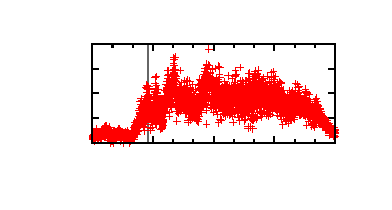
\includegraphics{/home/rik/workspace/ASL_student_project/Repositories/report-fork/Presentation/LaTeX_Template/images/windday}}%
    \gplfronttext
  \end{picture}%
\endgroup

	% GNUPLOT: LaTeX picture with Postscript
\begingroup
  \makeatletter
  \providecommand\color[2][]{%
    \GenericError{(gnuplot) \space\space\space\@spaces}{%
      Package color not loaded in conjunction with
      terminal option `colourtext'%
    }{See the gnuplot documentation for explanation.%
    }{Either use 'blacktext' in gnuplot or load the package
      color.sty in LaTeX.}%
    \renewcommand\color[2][]{}%
  }%
  \providecommand\includegraphics[2][]{%
    \GenericError{(gnuplot) \space\space\space\@spaces}{%
      Package graphicx or graphics not loaded%
    }{See the gnuplot documentation for explanation.%
    }{The gnuplot epslatex terminal needs graphicx.sty or graphics.sty.}%
    \renewcommand\includegraphics[2][]{}%
  }%
  \providecommand\rotatebox[2]{#2}%
  \@ifundefined{ifGPcolor}{%
    \newif\ifGPcolor
    \GPcolortrue
  }{}%
  \@ifundefined{ifGPblacktext}{%
    \newif\ifGPblacktext
    \GPblacktextfalse
  }{}%
  % define a \g@addto@macro without @ in the name:
  \let\gplgaddtomacro\g@addto@macro
  % define empty templates for all commands taking text:
  \gdef\gplbacktext{}%
  \gdef\gplfronttext{}%
  \makeatother
  \ifGPblacktext
    % no textcolor at all
    \def\colorrgb#1{}%
    \def\colorgray#1{}%
  \else
    % gray or color?
    \ifGPcolor
      \def\colorrgb#1{\color[rgb]{#1}}%
      \def\colorgray#1{\color[gray]{#1}}%
      \expandafter\def\csname LTw\endcsname{\color{white}}%
      \expandafter\def\csname LTb\endcsname{\color{black}}%
      \expandafter\def\csname LTa\endcsname{\color{black}}%
      \expandafter\def\csname LT0\endcsname{\color[rgb]{1,0,0}}%
      \expandafter\def\csname LT1\endcsname{\color[rgb]{0,1,0}}%
      \expandafter\def\csname LT2\endcsname{\color[rgb]{0,0,1}}%
      \expandafter\def\csname LT3\endcsname{\color[rgb]{1,0,1}}%
      \expandafter\def\csname LT4\endcsname{\color[rgb]{0,1,1}}%
      \expandafter\def\csname LT5\endcsname{\color[rgb]{1,1,0}}%
      \expandafter\def\csname LT6\endcsname{\color[rgb]{0,0,0}}%
      \expandafter\def\csname LT7\endcsname{\color[rgb]{1,0.3,0}}%
      \expandafter\def\csname LT8\endcsname{\color[rgb]{0.5,0.5,0.5}}%
    \else
      % gray
      \def\colorrgb#1{\color{black}}%
      \def\colorgray#1{\color[gray]{#1}}%
      \expandafter\def\csname LTw\endcsname{\color{white}}%
      \expandafter\def\csname LTb\endcsname{\color{black}}%
      \expandafter\def\csname LTa\endcsname{\color{black}}%
      \expandafter\def\csname LT0\endcsname{\color{black}}%
      \expandafter\def\csname LT1\endcsname{\color{black}}%
      \expandafter\def\csname LT2\endcsname{\color{black}}%
      \expandafter\def\csname LT3\endcsname{\color{black}}%
      \expandafter\def\csname LT4\endcsname{\color{black}}%
      \expandafter\def\csname LT5\endcsname{\color{black}}%
      \expandafter\def\csname LT6\endcsname{\color{black}}%
      \expandafter\def\csname LT7\endcsname{\color{black}}%
      \expandafter\def\csname LT8\endcsname{\color{black}}%
    \fi
  \fi
  \setlength{\unitlength}{0.0500bp}%
  \begin{picture}(3454.00,1700.00)%
    \gplgaddtomacro\gplbacktext{%
      \csname LTb\endcsname%
      \put(594,484){\makebox(0,0)[r]{\strut{} 0}}%
      \put(594,643){\makebox(0,0)[r]{\strut{} 2}}%
      \put(594,801){\makebox(0,0)[r]{\strut{} 4}}%
      \put(594,960){\makebox(0,0)[r]{\strut{} 6}}%
      \put(594,1118){\makebox(0,0)[r]{\strut{} 8}}%
      \put(594,1277){\makebox(0,0)[r]{\strut{} 10}}%
      \put(594,1435){\makebox(0,0)[r]{\strut{} 12}}%
      \put(726,264){\makebox(0,0){\strut{}30}}%
      \put(1503,264){\makebox(0,0){\strut{}31}}%
      \put(2280,264){\makebox(0,0){\strut{}32}}%
      \put(3057,264){\makebox(0,0){\strut{}33}}%
      \put(1891,154){\makebox(0,0){\strut{}time $[\si{\minute}]$}}%
    }%
    \gplgaddtomacro\gplfronttext{%
    }%
    \gplbacktext
    \put(0,0){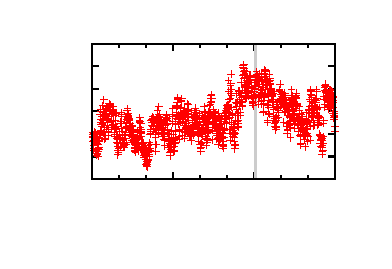
\includegraphics{/home/rik/workspace/ASL_student_project/Repositories/report-fork/Presentation/LaTeX_Template/images/windminute}}%
    \gplfronttext
  \end{picture}%
\endgroup

	\tiny{Wind speed observations in $[\si{\metre\per\second}$], \cite{www:googleheliostat}} 
	}
%    \def\figurewidth{{0.5\textwidth}}
%    \def\figureheight{0.6\figurewidth}
\end{minipage}

\clearpage
\ETHslide
\section*{System Overview}
%\addcontentsline{toc}{section}{Control Approach}
\vspace*{\fill}

\begin{figure}[h]
\centering
\scalebox{1}{
%\begin{tikzpicture}[auto, font=\small]
% coordinates
\coordinate (orig) at (0,0);
\coordinate (in1) at (0,-0.75);
\coordinate (in2) at (0,-1.75);
\coordinate (out1) at (12,-1.75/2);
\coordinate (LLA) at (1.5,-1.5);
\coordinate (LLB) at (4,-2.5);
\coordinate (LLC) at (6.5,-1.75);
\coordinate (LLD) at (9,-1.75);
\coordinate (in2inter1) at (1.5,-1.75);
\coordinate (out1inter1) at (11.5,-1.75/2);
\coordinate (out1inter2) at (3,-2.75);


% nodes
\node[draw, minimum width=1.5cm, minimum height=1.5cm, anchor=south west, text width=1.5cm, align=center] (A) at (LLA) {Position\\Control};
\node[draw, minimum width=1.5cm, minimum height=2cm, anchor=south west, text width=1.5cm, align=center] (B) at (LLB) {Attitude\\Control};
\node[draw, minimum width=1.5cm, minimum height=1.75cm, anchor=south west, text width=1.5cm, align=center] (C) at (LLC) {Allocation\\Map};
\node[draw, minimum width=1.5cm, minimum height=1.75cm, anchor=south west, text width=1.5cm, align=center] (D) at (LLD) {MAV\\Dynamics};

% edges
\draw[->] (in1) -- node[above] {$\mathbf{r}_{ref},\mathbf{v}_{ref}$} (A.180);

\draw[->] ($(A.0) + (0,0.5)$) -- node[above] {$T_{ref}$} ($(C.180) + (0,1.25/2)$);
\draw[->] (A.0) -- node[above] {$\phi_{ref}$} ($(B.180) + (0,0.75)$);
\draw[->] ($(A.0) - (0,0.5)$) -- node[above] {$\theta_{ref}$} ($(B.180) + (0,0.25)$);

\draw[-] (in2) -- node[above] {$\psi_{ref}$} (in2inter1);
\draw[->] (in2inter1) -- node {} ($(B.180) -  (0,0.25)$);

\draw[->] (B.0) -- node[above] {$\boldsymbol{\tau}_{ref}$} ($(C.180) - (0,1.25/2)$);

\draw[->] (C.0) -- node[above] {$\mathbf{n}_{ref}$} (D.180);

\draw[-] (D.0) -- node[] {} (out1inter1);
\path[fill] (out1inter1) circle[radius=1pt];
\draw[->] (out1inter1) -- node[] {} (out1);

\path[draw,-] (out1inter1) |- node[near end,below] {$\mathbf{r},\mathbf{v},\mathbf{q},\boldsymbol{\omega}$} (out1inter2) ;
\path[draw,->] (out1inter2) |- ($(B.180) - (0,0.75)$) ;
\path[draw,->] (out1inter2) -| ($(A.270)$) ;

%  %coordinates
%  \coordinate (orig)   at (0,0);
%  \coordinate (LLD)    at (4,0);
%  \coordinate (AroneA) at (-1/2,11/2);
%  \coordinate (ArtwoA) at (-1/2,5);
%  \coordinate (ArthrA) at (-1/2,9/2);
%  \coordinate (LLA)    at (1,4);
%  \coordinate (LLB)    at (4,4);
%  \coordinate (LLC)    at (7,4);
%  \coordinate (AroneC) at (25/2,11/2);
%  \coordinate (ArtwoC) at (25/2,5);
%  \coordinate (ArthrC) at (25/2,9/2);
%  \coordinate (conCBD) at (21/2,9/2);
%  \coordinate (conCB)  at (21/2,7/2);
%  \coordinate (coCBD)  at (11,5);
%  \coordinate (coCB)   at (11,3);
%  \coordinate (conCBA) at (23/2,11/2);
%  \coordinate (conCA)  at (23/2,5/2);
%%
%%  %nodes
%  \node[draw, minimum width=2cm, minimum height=2cm, anchor=south west, text width=2cm, align=center] (A) at (LLA) {Impedance\\control};
%  \node[draw, minimum width=2cm, minimum height=2cm, anchor=south west, text width=2cm, align=center] (B) at (LLB) {Inverse\\Dynamics};
%  \node[draw, minimum width=3cm, minimum height=2cm, anchor=south west, text width=2cm, align=center] (C) at (LLC) {Manipulator\\and\\environment};
%  \node[draw, minimum width=2cm, minimum height=2cm, anchor=south west, text width=2cm, align=center] (D) at (LLD) {Direct\\kinematics};
%
%  %edges
%  \draw[->] (AroneA) -- node[above]{$p_d, R_d$} ($(A.180) + (0,1/2)$);
%  \draw[->] (ArtwoA) -- node[above]{$v_d$} (A.180);
%  \draw[->] (ArthrA) -- node[above]{$v_d$} ($(A.180) + (0,-1/2)$);
%
%  \draw[->] (A.0) -- node[above] {$\alpha$} (B.180);
%  \draw[->] (B.0) -- node[above] {$\tau$} (C.180);
%
%  \draw[->] ($(C.0) + (0,1/2)$) -- node[above, pos=0.2]{$h_e$} (AroneC);
%  \draw[->] (C.0) -- node[above, pos=0.2]{$q$} (ArtwoC);
%  \draw[->] ($(C.0) + (0,-1/2)$) -- node[above, pos=0.2]{$q$} (ArthrC);
%
%  \path[fill] (conCBD) circle[radius=1pt] (conCB) circle[radius=1pt];
%  \path[draw,->] (conCBD) -- (conCB) -| ($(B.270) + (1/2,0)$);
%
%  \path[fill] (coCBD) circle[radius=1pt] (coCB) circle[radius=1pt];
%  \path[draw,->] (coCBD)  -- (coCB) -| (B.270);
%
%  \path[fill] (conCBA) circle[radius=1pt] (conCA) circle[radius=1pt];
%  \path[draw,->] (conCBA) -- (conCA) -| ($(B.270) + (-1/2,0)$);
%
%  \path[draw,->] (conCB) |- ($(D.0) + (0,1/2)$);
%  \path[draw,->] (coCB)  |- ($(D.0) + (0,-1/2)$);
%
%  \path[draw,->] (conCA) |- ($(A.270) + (-1/2,0) + (0,-9/2)$) -- ($(A.270) + (-1/2,0)$);
%
%  \path[draw,->] ($(D.180) + (0,1/2)$)  -| node[above,pos=0.2] {$p_e,r_e$} ($(A.270) + (1/2,0)$);
%  \path[draw,->] ($(D.180) + (0,-1/2)$) -| node[above,pos=0.15] {$v_e$} (A.270);

\end{tikzpicture}

\begin{tikzpicture}[auto, font=\small]
% coordinates
\coordinate (orig) at (0,0);
\coordinate (LLA) at (2,0);
\coordinate (LLB) at (5.5,0);
\coordinate (outinter) at (8,0);
\coordinate (out) at (9,0);


% nodes
\node[draw, minimum width=1.5cm, minimum height=1.5cm, anchor=west, text width=1.5cm, align=center] (A) at (LLA) {Position\\Control};
\node[draw, minimum width=1.5cm, minimum height=1.5cm, anchor=west, text width=1.5cm, align=center,fill=black,opacity=0.6] (B) at (LLB) {MAV \\Black Box};

% edges
\draw[->] (orig) -- node[above] {$\mathbf{r}_{ref},\mathbf{v}_{ref},\psi_{ref}$} (A.180);
\draw[->] (A.0) -- node[above] {$\begin{bmatrix}
T_{ref} \\ \phi_{ref} \\ \theta_{ref} \\ \psi_{ref}
\end{bmatrix}$} (B.180);
\draw[->] (B.0) -- (out);
\coordinate (feedback) at ($(A.270)-(0,0.75)$);
\draw[-] (outinter) |- node[above,near end] {$\mathbf{r},\mathbf{v},\mathbf{q},\boldsymbol{\omega},\mathbf{w}$} (feedback);
\draw[->] (feedback) -- (A.270);

\end{tikzpicture}

}
\end{figure}
\begin{itemize}
\item[\ETHitem] Cascaded control
\item[\ETHitem] Given attitude control
\item[\ETHitem] Given state and wind estimation
\item[\ETHitem] SysId attitude and thrust dynamics
\end{itemize}

\vspace*{\fill}
\clearpage
\ETHslide
\section*{Control System}
%\addcontentsline{toc}{section}{Control System}
\vspace*{\fill}
\begin{figure}[h]
\centering
\scalebox{0.5}{
\begin{tikzpicture}[auto, font=\small]
% coordinates
\coordinate (orig) at (0,0);
% inputs
\coordinate (Tin) at (orig);
\coordinate (phiin) at ($(orig)- (0,1.75)$);
\coordinate (thetain) at ($(phiin)- (0,1.75)$);
\coordinate (psiin) at ($(thetain)- (0,1.75)$);
% boxes
\coordinate (LLA) at ($(Tin) + (0.75,-0.75)$);
\coordinate (LLB) at ($(phiin) + (0.75,-0.75)$);
\coordinate (LLC) at ($(thetain) + (0.75,-0.75)$);
\coordinate (LLD) at ($(LLC) + (1.5+1.25,0)$);

% nodes
% boxes
\node[draw,minimum width=1.5cm, minimum height=1.5cm, anchor=south west, text width=1.5cm, align=center] (A) at (LLA) {$\Large 1$};
\node[draw,minimum width=1.5cm, minimum height=1.5cm, anchor=south west, text width=1.5cm, align=center] (B) at (LLB) {$2$nd Order};
\node[draw,minimum width=1.5cm, minimum height=1.5cm, anchor=south west, text width=1.5cm, align=center] (C) at (LLC) {$2$nd Order};
\node[draw,minimum width=3cm, minimum height=3.25cm, anchor=south west, align=center] (D) at (LLD) {Newton\\
Law};

\node[draw,minimum width=0.75cm, minimum height=0.75cm, anchor=west, text width=0.75cm, align=center] (E) at ($(D.0) + (0.5,0)$) {$\Large \int$};
\node[draw,minimum width=0.75cm, minimum height=0.75cm, anchor=west, text width=0.75cm, align=center] (F) at ($(E.0) + (0.5,0)$) {$\Large \int$};
% coordinates at boxes
\coordinate (DTin) at ($(D.180) + (0,2*0.55)$);
\coordinate (Dphiin) at ($(D.180) + (0,1*0.55)$);
\coordinate (Dthetain) at ($(D.180)$);
\coordinate (Dpsiin) at ($(D.180) - (0,1*0.55)$);
\coordinate (Ddxin) at ($(D.180) - (0,2*0.55)$);
\coordinate[above=of D.90] (win);
%lines
\draw[->] (Tin) -- node[at start,above]{$T_{ref}$} (A.180);
\draw[->] (phiin) -- node[at start,above]{$\phi_{ref}$} (B.180);
\draw[->] (thetain) -- node[at start,above]{$\theta_{ref}$} (C.180);
\draw[->] (A.0) -| node[near start,above]{$T$} ($(DTin) - (0.5,0)$) -- (DTin);
\draw[->] (B.0) -| node[near start,above]{$\phi$} ($(Dphiin) - (0.5,0)$) --  (Dphiin);
\draw[->] (C.0) -| node[near start,above]{$\theta$} ($(Dthetain) - (0.75,0)$) -- (Dthetain);
\draw[->] (psiin) -| node[at start,above]{$\psi_{m}$} ($(Dpsiin) - (0.5,0)$) -- (Dpsiin);

\draw[->] (D.0) -- node[above]{${\mathbf{a}}$} (E.180);
\draw[->] (E.0) -- node[above]{${\mathbf{v}}$} (F.180);
\coordinate (out) at ($(F.0) + (0.5,0)$);
\draw[->] (F.0) -- node[above]{$\mathbf{r}$} (out);

\draw[->] ($(E.0) + (0.5/2,0)$) |- ($(D.south west) - (0.25,0.5)$) |- (Ddxin);

\draw[->] (win) node[above]{$\E[\mathbf{w}]$}  -- (D.90);


\end{tikzpicture}

}
\end{figure}
\tiny{
\begin{align}
f\left(\mathbf{x},\mathbf{u},\mathbf{w}\right) &= \ddt \mathbf{x}  
= \begin{bmatrix}
\mathbf{A}_\phi \begin{bmatrix}
\frac{1}{8}\dot{\phi} \\ \phi
\end{bmatrix}
+ \mathbf{B}_\phi \phi_{ref} \\
\mathbf{A}_\theta \begin{bmatrix}
\frac{1}{8}\dot{\theta} \\ \theta
\end{bmatrix}
+ \mathbf{B}_\theta \theta_{ref} \\
\mathbf{v}\\
\frac{1}{m} \left( \mathbf{F}_{T,total} + \mathbf{F}_{D,total} \right)  + \begin{bmatrix}
0 \\ 0 \\ -g
\end{bmatrix} 
\end{bmatrix} \nonumber
\end{align}
}
\normalsize{}

%\begin{minipage}{0.6\textwidth}
%\end{minipage}
%\begin{minipage}{0.39\textwidth}
%\end{minipage}

\vspace*{\fill}
\clearpage
\addcontentsline{toc}{section}{Control}
\ETHslide
\section*{Receding Horizon Control}
%\addcontentsline{toc}{section}{}
\vspace*{\fill}

\begin{figure}[h]
\centering
\scalebox{0.6}{
\begin{tikzpicture}[auto, font=\small]
% coordinates
\coordinate (orig) at (0,0);
\coordinate (LLA) at (orig);
\coordinate (LLB) at (6.5,0);
\coordinate (out) at (12.5,0);


% nodes
\node[draw, minimum width=5cm, minimum height = 4cm, anchor=west, text width=5cm,align=center] (A) at (LLA) {\begin{align*}
&\argmin_{U_t}&  &\sum_{k=0}^{N-1} q(x_{t+k},u_{t+k}) \\
&\text{s.t.}  &  &x_t = x(t) \\
&	          &  &x_{t+k+1} = Ax_{t+k} + Bu_{t+k} \\
&	          &  &x_{t+k}\in\mathcal{X}, \; u_{t+k}\in\mathcal{U}
\end{align*}};
\node[draw, minimum width=4cm, minimum height = 4cm, anchor=west, text width=4cm,align=center] (B) at (LLB) {\Huge{\text{Plant}}};

% edges
\draw[->] (A.0) -- node[above] {$u^*_t$} (B.180);
\draw[->] (B.0) -- node[above] {Output $y(t)$} (out);
\coordinate (stateinter) at ($(A.270) - (0,1)$);
\draw[-] (B.270) |- node[near end, above] {State $x(t)$} (stateinter);
\draw[->] (stateinter) -- (A.270);


% edges
%\draw[->] (in1) -- node[above] {$\mathbf{r}_{ref},\mathbf{v}_{ref}$} (A.180);
%
%\draw[->] ($(A.0) + (0,0.5)$) -- node[above] {$T_{ref}$} ($(C.180) + (0,1.25/2)$);
%\draw[->] (A.0) -- node[above] {$\phi_{ref}$} ($(B.180) + (0,0.75)$);
%\draw[->] ($(A.0) - (0,0.5)$) -- node[above] {$\theta_{ref}$} ($(B.180) + (0,0.25)$);
%
%\draw[-] (in2) -- node[above] {$\psi_{ref}$} (in2inter1);
%\draw[->] (in2inter1) -- node {} ($(B.180) -  (0,0.25)$);
%
%\draw[->] (B.0) -- node[above] {$\boldsymbol{\tau}_{ref}$} ($(C.180) - (0,1.25/2)$);
%
%\draw[->] (C.0) -- node[above] {$\mathbf{n}_{ref}$} (D.180);
%
%\draw[-] (D.0) -- node[] {} (out1inter1);
%\path[fill] (out1inter1) circle[radius=1pt];
%\draw[->] (out1inter1) -- node[] {} (out1);
%
%\path[draw,-] (out1inter1) |- node[near end,below] {$\mathbf{x},\mathbf{\dot{x}},\mathbf{q},\boldsymbol{\omega}$} (out1inter2) ;
%\path[draw,->] (out1inter2) |- ($(B.180) - (0,0.75)$) ;
%\path[draw,->] (out1inter2) -| ($(A.270)$) ;

\end{tikzpicture}
}
\end{figure} 
At each sample time:
\begin{itemize}
\item[\ETHitem] Measure/estimate current state $x(t)$
\item[\ETHitem] Find the optimal input sequence for the entire planning window $N$: $U_t^* = \{ u_t^*, u_{t+1}^*, \ldots, u_{t+N-1}^* \}$
\item[\ETHitem] Implement the first control action $u_t^*$
\end{itemize}

\vspace*{\fill}
\clearpage
\ETHslide
\section*{Receding Horizon Control}
%\addcontentsline{toc}{section}{}
\vspace*{\fill}

Advantages:
\begin{itemize}
\item[\ETHitem] Input and output constraints
\item[\ETHitem] Predictive
\item[\ETHitem] Intuitive
\end{itemize}
Disadvantages:
\begin{itemize}
\item[\ETHitem] No robustness guarantees
\item[\ETHitem] OCP computationally expensive
\end{itemize}

\vspace*{\fill}
\clearpage
\ETHslide
\section*{Linear and nonlinear MPC}
\vspace*{\fill}

\begin{itemize}
\item[\ETHitem] deterministic wind feed-forward
\item[\ETHitem] offset-free constant reference tracking
\item[\ETHitem] trajectory tracking
\end{itemize}

Difference:
\begin{itemize}
\item[\ETHitem] MPC linearization about hovering
\item[\ETHitem] NMPC nonlinear dynamics
\end{itemize}

\vspace*{\fill}
\clearpage
\addcontentsline{toc}{section}{Simulation}
\ETHslide
\section*{Nonlinear MPC OCP}
%\addcontentsline{toc}{section}{}
\vspace*{\fill}
\footnotesize{
\begin{align}
&\min_{x(\cdot),u(\cdot)} &&\int_{t}^{t+NT_s} \left( ||x(\tau)-x_{ref}(\tau)||_Q^2 + ||u(\tau)-u_{ref}(\tau)||_R^2 \d \tau \right)  \nonumber \\
&&&+ ||x(t+NT_s)-x_{ref}(t+NT_s)||_P^2 \nonumber \\
&s.t. &&\dot{x}(\tau) = f(x(\tau),u(\tau),w(\tau),\psi(\tau)) \nonumber \\
&&&\dot{w}(\tau) = 0 \nonumber \\
&&&\dot{\psi}(\tau) = 0 \nonumber \\
&&&\begin{bmatrix}
T_{min} \\ -45 \si{\degree} \\-45 \si{\degree}
\end{bmatrix} \leq u(\tau) \leq \begin{bmatrix}
T_{max} \\ 45 \si{\degree} \\45 \si{\degree}
\end{bmatrix} , \quad \forall\tau\in\left[t,t+NT_s\right] \nonumber \\
&&&x(t) = \hat{x}(t),\; w(t) = \hat{w}(t), \; \psi(t) = \hat{\psi}(t)  \nonumber \\
&&&N=100\nonumber
\end{align}
}
\normalsize{}
\vspace*{\fill}
\clearpage
\ETHslide
\section*{Step Response: Nonlinear MPC}
%\addcontentsline{toc}{section}{}
\vspace*{\fill}

\begin{minipage}{0.5\textwidth}
	\centering
	\tiny{
	% This file was created by matlab2tikz.
% Minimal pgfplots version: 1.3
%
\definecolor{mycolor1}{rgb}{0.00000,0.44700,0.74100}%
\definecolor{mycolor2}{rgb}{0.85000,0.32500,0.09800}%
\definecolor{mycolor3}{rgb}{0.92900,0.69400,0.12500}%
%
\begin{tikzpicture}

\begin{axis}[%
width=\figurewidth,
height=0.984009\figureheight,
at={(0\figurewidth,0\figureheight)},
scale only axis,
xmin=0,
xmax=5,
xlabel={time $[\si{\second}]$},
ymin=-0.2,
ymax=1.2,
ylabel={position $[\si{\metre}]$},
axis x line*=bottom,
axis y line*=left,
legend style={at={(0.5,1.03)},anchor=south,legend columns=3,legend cell align=left,align=left,draw=white!15!black}
]
\addplot [color=mycolor1,solid]
  table[row sep=crcr]{%
0	0\\
0.01	1.60581295478493e-08\\
0.02	5.5087181778581e-07\\
0.03	4.05601948648053e-06\\
0.04	1.61411753450517e-05\\
0.05	4.60030347273778e-05\\
0.06	0.000106609936769602\\
0.07	0.000214642775983744\\
0.08	0.000390252282350667\\
0.09	0.000656711033571038\\
0.1	0.0010400077588092\\
0.11	0.00156841677740011\\
0.12	0.00227206187317352\\
0.13	0.00318249091433643\\
0.14	0.00433226247854473\\
0.15	0.00575454717447387\\
0.16	0.00748274683924581\\
0.17	0.00955013555443752\\
0.18	0.0119895258850874\\
0.19	0.0148329627953943\\
0.2	0.0181114538218729\\
0.21	0.0218547420962327\\
0.22	0.0260911178862742\\
0.23	0.0308472694701721\\
0.24	0.0361481831811439\\
0.25	0.0420170965381255\\
0.26	0.0484754577821703\\
0.27	0.055542906472502\\
0.28	0.0632373056317423\\
0.29	0.0715772267287005\\
0.3	0.0805855866798955\\
0.31	0.090280087611057\\
0.32	0.100675903207807\\
0.33	0.111801367601804\\
0.34	0.123679028216549\\
0.35	0.136313222957489\\
0.36	0.149698525747945\\
0.37	0.163821507265484\\
0.38	0.178656899467097\\
0.39	0.194169405407068\\
0.4	0.21032536784312\\
0.41	0.227094246090643\\
0.42	0.244445234379705\\
0.43	0.262345333665308\\
0.44	0.280758500793248\\
0.45	0.299645512815447\\
0.46	0.318964227943006\\
0.47	0.338670001591881\\
0.48	0.358716131717928\\
0.49	0.379054279372711\\
0.5	0.399634852400628\\
0.51	0.420407359337045\\
0.52	0.441320742485432\\
0.53	0.46232369699858\\
0.54	0.483364975573142\\
0.55	0.504393682174318\\
0.56	0.525359562161288\\
0.57	0.546213159105915\\
0.58	0.56690571373642\\
0.59	0.587389596065393\\
0.6	0.607619145927036\\
0.61	0.627551572597063\\
0.62	0.647147697224647\\
0.63	0.666372418808208\\
0.64	0.68519488921961\\
0.65	0.703588498875233\\
0.66	0.721530715171683\\
0.67	0.739002446356348\\
0.68	0.755986918092086\\
0.69	0.772469541242334\\
0.7	0.788438435748595\\
0.71	0.803884660935874\\
0.72	0.818802239384977\\
0.73	0.833188058931503\\
0.74	0.847041694314639\\
0.75	0.860365173349219\\
0.76	0.873162705165154\\
0.77	0.885440385065788\\
0.78	0.897205889613629\\
0.79	0.908468174939915\\
0.8	0.919237189984287\\
0.81	0.929523614200206\\
0.82	0.93933862652034\\
0.83	0.948693709519204\\
0.84	0.95760049010972\\
0.85	0.966070615975282\\
0.86	0.974115663552813\\
0.87	0.981747058503678\\
0.88	0.988976028167798\\
0.89	0.995813587939131\\
0.9	1.00227053780373\\
0.91	1.00835748636401\\
0.92	1.0140849209632\\
0.93	1.01946328085409\\
0.94	1.02450300251779\\
0.95	1.02921452765575\\
0.96	1.03360829000045\\
0.97	1.03769469618058\\
0.98	1.04148411203983\\
0.99	1.04498686301412\\
1	1.04821323861647\\
1.01	1.05117349139298\\
1.02	1.05387782699344\\
1.03	1.05633638640416\\
1.04	1.0585592239242\\
1.05	1.06055628344465\\
1.06	1.06233737481409\\
1.07	1.06391215122054\\
1.08	1.06529008845579\\
1.09	1.06648046712945\\
1.1	1.06749235823733\\
1.11	1.06833461208248\\
1.12	1.06901584987431\\
1.13	1.06954445740875\\
1.14	1.06992858198651\\
1.15	1.07017613303664\\
1.16	1.07029478506801\\
1.17	1.07029198182129\\
1.18	1.07017494081065\\
1.19	1.06995065814171\\
1.2	1.06962591307332\\
1.21	1.06920727227928\\
1.22	1.06870109388721\\
1.23	1.06811353130592\\
1.24	1.06745053682476\\
1.25	1.0667178649593\\
1.26	1.06592107551246\\
1.27	1.06506553637034\\
1.28	1.06415642607333\\
1.29	1.06319873611414\\
1.3	1.06219727300165\\
1.31	1.06115666015959\\
1.32	1.06008133965078\\
1.33	1.05897557377921\\
1.34	1.05784344663958\\
1.35	1.0566888656343\\
1.36	1.05551556300645\\
1.37	1.05432709743323\\
1.38	1.05312685571886\\
1.39	1.05191805462381\\
1.4	1.05070374286663\\
1.41	1.04948680332879\\
1.42	1.04826995550107\\
1.43	1.04705575815389\\
1.44	1.04584661221272\\
1.45	1.04464476383218\\
1.46	1.04345230766356\\
1.47	1.04227119030613\\
1.48	1.04110321393088\\
1.49	1.03995004006313\\
1.5	1.03881319351005\\
1.51	1.03769406641802\\
1.52	1.03659392244443\\
1.53	1.03551390102855\\
1.54	1.03445502174577\\
1.55	1.03341818872982\\
1.56	1.03240419514805\\
1.57	1.03141372771491\\
1.58	1.03044737122975\\
1.59	1.02950561312537\\
1.6	1.02858884801446\\
1.61	1.02769738222197\\
1.62	1.02683143829181\\
1.63	1.02599115945756\\
1.64	1.02517661406696\\
1.65	1.02438779995122\\
1.66	1.02362464873059\\
1.67	1.02288703004844\\
1.68	1.02217475572657\\
1.69	1.02148758383547\\
1.7	1.0208252226734\\
1.71	1.02018733464901\\
1.72	1.01957354006273\\
1.73	1.01898342078255\\
1.74	1.01841652381051\\
1.75	1.01787236473845\\
1.76	1.01735043108691\\
1.77	1.01685018552449\\
1.78	1.01637106896827\\
1.79	1.01591250356246\\
1.8	1.0154738955339\\
1.81	1.01505463792366\\
1.82	1.01465411319442\\
1.83	1.01427169571129\\
1.84	1.01390675409674\\
1.85	1.01355865346122\\
1.86	1.0132267575106\\
1.87	1.01291043053063\\
1.88	1.01260903924744\\
1.89	1.01232195456763\\
1.9	1.0120485532007\\
1.91	1.01178821916376\\
1.92	1.01154034517059\\
1.93	1.01130433390996\\
1.94	1.01107959921222\\
1.95	1.01086556711061\\
1.96	1.0106616767972\\
1.97	1.01046738147864\\
1.98	1.01028214913469\\
1.99	1.01010546318278\\
2	1.00993682305247\\
2.01	1.00977574467144\\
2.02	1.00962176086742\\
2.03	1.00947442168892\\
2.04	1.00933329464677\\
2.05	1.0091979648787\\
2.06	1.00906803524046\\
2.07	1.00894312632692\\
2.08	1.00882287642756\\
2.09	1.00870694142064\\
2.1	1.00859499461057\\
2.11	1.00848672651339\\
2.12	1.00838184459473\\
2.13	1.00828007296507\\
2.14	1.00818115203672\\
2.15	1.00808483814674\\
2.16	1.00799090315011\\
2.17	1.00789913398685\\
2.18	1.00780933222693\\
2.19	1.00772131359632\\
2.2	1.00763490748762\\
2.21	1.00754995645731\\
2.22	1.00746631571065\\
2.23	1.00738385257689\\
2.24	1.00730244597835\\
2.25	1.0072219858972\\
2.26	1.00714237284295\\
2.27	1.00706351732324\\
2.28	1.00698533931991\\
2.29	1.00690776777192\\
2.3	1.00683074006644\\
2.31	1.00675420153897\\
2.32	1.00667810498336\\
2.33	1.00660241017255\\
2.34	1.0065270833905\\
2.35	1.00645209697614\\
2.36	1.00637742887951\\
2.37	1.00630306223093\\
2.38	1.00622898492334\\
2.39	1.00615518920865\\
2.4	1.00608167130821\\
2.41	1.00600843103793\\
2.42	1.00593547144844\\
2.43	1.00586279848037\\
2.44	1.0057904206352\\
2.45	1.00571834866173\\
2.46	1.00564659525833\\
2.47	1.00557517479109\\
2.48	1.00550410302775\\
2.49	1.00543339688755\\
2.5	1.00536307420677\\
2.51	1.00529315351973\\
2.52	1.00522365385532\\
2.53	1.00515459454843\\
2.54	1.00508599506627\\
2.55	1.00501787484908\\
2.56	1.00495025316478\\
2.57	1.00488314897735\\
2.58	1.00481658082823\\
2.59	1.00475056673035\\
2.6	1.00468512407435\\
2.61	1.00462026954631\\
2.62	1.00455601905655\\
2.63	1.0044923876789\\
2.64	1.00442938959992\\
2.65	1.00436703807748\\
2.66	1.00430534540796\\
2.67	1.00424432290188\\
2.68	1.00418398086851\\
2.69	1.00412432861003\\
2.7	1.0040653744234\\
2.71	1.00400712560804\\
2.72	1.00394958847754\\
2.73	1.00389276837483\\
2.74	1.00383666969012\\
2.75	1.00378129588136\\
2.76	1.00372664949709\\
2.77	1.00367273220133\\
2.78	1.00361954480059\\
2.79	1.00356708727271\\
2.8	1.00351535879739\\
2.81	1.00346435778828\\
2.82	1.0034140819265\\
2.83	1.00336452819522\\
2.84	1.00331569291533\\
2.85	1.00326757178185\\
2.86	1.00322015990089\\
2.87	1.00317345182704\\
2.88	1.00312744160092\\
2.89	1.0030821227867\\
2.9	1.0030374885095\\
2.91	1.00299353149238\\
2.92	1.0029502440928\\
2.93	1.00290761833849\\
2.94	1.00286564596248\\
2.95	1.00282431843716\\
2.96	1.00278362700743\\
2.97	1.0027435627226\\
2.98	1.0027041164672\\
2.99	1.00266527899042\\
3	1.00262704093426\\
3.01	1.00258939286029\\
3.02	1.00255232527502\\
3.03	1.00251582865378\\
3.04	1.00247989346316\\
3.05	1.00244451018205\\
3.06	1.00240966932113\\
3.07	1.00237536144097\\
3.08	1.00234157716869\\
3.09	1.00230830721324\\
3.1	1.00227554237926\\
3.11	1.00224327357965\\
3.12	1.00221149184683\\
3.13	1.00218018834274\\
3.14	1.00214935436766\\
3.15	1.00211898136784\\
3.16	1.00208906094211\\
3.17	1.00205958484732\\
3.18	1.00203054500295\\
3.19	1.00200193349463\\
3.2	1.0019737425769\\
3.21	1.00194596467513\\
3.22	1.00191859238661\\
3.23	1.00189161848105\\
3.24	1.00186503590033\\
3.25	1.00183883775773\\
3.26	1.00181301733655\\
3.27	1.00178756808833\\
3.28	1.00176248363053\\
3.29	1.00173775774388\\
3.3	1.00171338436938\\
3.31	1.00168935760499\\
3.32	1.00166567170205\\
3.33	1.00164232106145\\
3.34	1.0016193002297\\
3.35	1.0015966038948\\
3.36	1.00157422688194\\
3.37	1.00155216414923\\
3.38	1.00153041078325\\
3.39	1.0015089619947\\
3.4	1.0014878131139\\
3.41	1.0014669595864\\
3.42	1.00144639696864\\
3.43	1.00142612092353\\
3.44	1.00140612721627\\
3.45	1.00138641171012\\
3.46	1.00136697036236\\
3.47	1.00134779922023\\
3.48	1.00132889441717\\
3.49	1.00131025216897\\
3.5	1.00129186877022\\
3.51	1.00127374059083\\
3.52	1.00125586407264\\
3.53	1.00123823572627\\
3.54	1.00122085212802\\
3.55	1.00120370991698\\
3.56	1.00118680579225\\
3.57	1.0011701365103\\
3.58	1.00115369888249\\
3.59	1.00113748977274\\
3.6	1.00112150609528\\
3.61	1.0011057448126\\
3.62	1.00109020293349\\
3.63	1.00107487751124\\
3.64	1.00105976564188\\
3.65	1.00104486446266\\
3.66	1.00103017115056\\
3.67	1.00101568292092\\
3.68	1.00100139702615\\
3.69	1.00098731075464\\
3.7	1.00097342142963\\
3.71	1.00095972640821\\
3.72	1.0009462230805\\
3.73	1.00093290886874\\
3.74	1.00091978122659\\
3.75	1.0009068376384\\
3.76	1.00089407561863\\
3.77	1.00088149271127\\
3.78	1.00086908648931\\
3.79	1.00085685455428\\
3.8	1.00084479453585\\
3.81	1.00083290409141\\
3.82	1.00082118090579\\
3.83	1.00080962269088\\
3.84	1.00079822718538\\
3.85	1.00078699215455\\
3.86	1.00077591538997\\
3.87	1.00076499470933\\
3.88	1.00075422795622\\
3.89	1.00074361299996\\
3.9	1.00073314773543\\
3.91	1.00072283008293\\
3.92	1.000712657988\\
3.93	1.00070262942127\\
3.94	1.00069274237836\\
3.95	1.00068299487972\\
3.96	1.00067338497049\\
3.97	1.00066391072037\\
3.98	1.0006545702235\\
3.99	1.00064536159829\\
4	1.00063628298732\\
4.01	1.00062733255719\\
4.02	1.00061850849834\\
4.03	1.00060980902494\\
4.04	1.00060123237472\\
4.05	1.00059277680881\\
4.06	1.00058444061159\\
4.07	1.0005762220905\\
4.08	1.00056811957586\\
4.09	1.00056013142072\\
4.1	1.00055225600066\\
4.11	1.00054449171358\\
4.12	1.00053683697953\\
4.13	1.00052929024049\\
4.14	1.00052184996016\\
4.15	1.00051451462378\\
4.16	1.00050728273788\\
4.17	1.00050015283006\\
4.18	1.00049312344879\\
4.19	1.00048619316317\\
4.2	1.00047936056268\\
4.21	1.00047262425698\\
4.22	1.00046598287565\\
4.23	1.00045943506794\\
4.24	1.00045297950257\\
4.25	1.00044661486744\\
4.26	1.00044033986941\\
4.27	1.00043415323405\\
4.28	1.00042805370539\\
4.29	1.00042204004568\\
4.3	1.00041611103515\\
4.31	1.00041026547171\\
4.32	1.0004045021708\\
4.33	1.00039881996509\\
4.34	1.00039321770431\\
4.35	1.000387694255\\
4.36	1.00038224850033\\
4.37	1.00037687933989\\
4.38	1.0003715856894\\
4.39	1.00036636648049\\
4.4	1.00036122066043\\
4.41	1.00035614719184\\
4.42	1.00035114505245\\
4.43	1.00034621323478\\
4.44	1.00034135074594\\
4.45	1.00033655660734\\
4.46	1.00033182985442\\
4.47	1.00032716953647\\
4.48	1.00032257471633\\
4.49	1.00031804447022\\
4.5	1.00031357788752\\
4.51	1.00030917407054\\
4.52	1.00030483213436\\
4.53	1.00030055120662\\
4.54	1.00029633042734\\
4.55	1.00029216894877\\
4.56	1.00028806593518\\
4.57	1.00028402056272\\
4.58	1.00028003201924\\
4.59	1.00027609950414\\
4.6	1.00027222222822\\
4.61	1.00026839941351\\
4.62	1.00026463029308\\
4.63	1.00026091411097\\
4.64	1.00025725012195\\
4.65	1.00025363759141\\
4.66	1.00025007579523\\
4.67	1.00024656401957\\
4.68	1.00024310156075\\
4.69	1.00023968772514\\
4.7	1.00023632182894\\
4.71	1.00023300319809\\
4.72	1.00022973116811\\
4.73	1.00022650508395\\
4.74	1.00022332429985\\
4.75	1.00022018817922\\
4.76	1.00021709609449\\
4.77	1.00021404742697\\
4.78	1.00021104156672\\
4.79	1.00020807791245\\
4.8	1.00020515587133\\
4.81	1.00020227485894\\
4.82	1.00019943429909\\
4.83	1.00019663362371\\
4.84	1.00019387227276\\
4.85	1.00019114969407\\
4.86	1.00018846534326\\
4.87	1.00018581868363\\
4.88	1.00018320918599\\
4.89	1.00018063632864\\
4.9	1.00017809959719\\
4.91	1.0001755984845\\
4.92	1.00017313249054\\
4.93	1.00017070112233\\
4.94	1.00016830389379\\
4.95	1.00016594032568\\
4.96	1.00016360994551\\
4.97	1.00016131228739\\
4.98	1.000159046892\\
4.99	1.00015681330645\\
5	1.00015461108421\\
};
\addlegendentry{x};

\addplot [color=mycolor2,solid]
  table[row sep=crcr]{%
0	0\\
0.01	2.8323325738726e-23\\
0.02	5.09196865424944e-22\\
0.03	3.30036251167033e-21\\
0.04	1.276389955847e-20\\
0.05	3.50480267829621e-20\\
0.06	7.75594304116597e-20\\
0.07	1.48616326105995e-19\\
0.08	2.57080954195957e-19\\
0.09	4.12232629487576e-19\\
0.1	6.23649816011453e-19\\
0.11	9.01140748498015e-19\\
0.12	1.25455767760856e-18\\
0.13	1.69374910375674e-18\\
0.14	2.22854902144727e-18\\
0.15	2.86737212980385e-18\\
0.16	3.61409519593669e-18\\
0.17	4.46707800069458e-18\\
0.18	5.4182811464254e-18\\
0.19	6.45498813461591e-18\\
0.2	7.56189336536773e-18\\
0.21	8.72144144148362e-18\\
0.22	9.91628989903581e-18\\
0.23	1.11326424889836e-17\\
0.24	1.23604011492855e-17\\
0.25	1.35938190506929e-17\\
0.26	1.48310918082124e-17\\
0.27	1.60730509500562e-17\\
0.28	1.73223189812884e-17\\
0.29	1.85824594083525e-17\\
0.3	1.9857074582718e-17\\
0.31	2.11476369996861e-17\\
0.32	2.24501798012657e-17\\
0.33	2.37557173544026e-17\\
0.34	2.50514651550396e-17\\
0.35	2.63226060797095e-17\\
0.36	2.75536927614738e-17\\
0.37	2.8729637757826e-17\\
0.38	2.98367431378018e-17\\
0.39	3.08633966324081e-17\\
0.4	3.17993435090381e-17\\
0.41	3.2634793802927e-17\\
0.42	3.33602599605366e-17\\
0.43	3.39661528384277e-17\\
0.44	3.44434066733327e-17\\
0.45	3.47847430159296e-17\\
0.46	3.4984821981224e-17\\
0.47	3.50400764070887e-17\\
0.48	3.49485549699242e-17\\
0.49	3.4709484127269e-17\\
0.5	3.43229487627963e-17\\
0.51	3.37897382019763e-17\\
0.52	3.31110877168959e-17\\
0.53	3.22887873928535e-17\\
0.54	3.13256279942475e-17\\
0.55	3.02254446966521e-17\\
0.56	2.89928451241173e-17\\
0.57	2.76331395962588e-17\\
0.58	2.61527279346517e-17\\
0.59	2.45595701672396e-17\\
0.6	2.28624515943031e-17\\
0.61	2.10708544583505e-17\\
0.62	1.91951677487286e-17\\
0.63	1.72465052124538e-17\\
0.64	1.52317093716278e-17\\
0.65	1.31449315703221e-17\\
0.66	1.09743624810821e-17\\
0.67	8.70558742631312e-18\\
0.68	6.32597689850055e-18\\
0.69	3.82843276279595e-18\\
0.7	1.21187272942432e-18\\
0.71	-1.51920613151842e-18\\
0.72	-4.35349444281211e-18\\
0.73	-7.27332413382112e-18\\
0.74	-1.02559081435645e-17\\
0.75	-1.3274730444483e-17\\
0.76	-1.63009955239864e-17\\
0.77	-1.93044472437221e-17\\
0.78	-2.22538014564865e-17\\
0.79	-2.511777797269e-17\\
0.8	-2.78678135605959e-17\\
0.81	-3.04783076766991e-17\\
0.82	-3.29265728464633e-17\\
0.83	-3.51927076717233e-17\\
0.84	-3.72594763487918e-17\\
0.85	-3.91121716506417e-17\\
0.86	-4.07382601349447e-17\\
0.87	-4.21272439343043e-17\\
0.88	-4.3271533839549e-17\\
0.89	-4.41665632188794e-17\\
0.9	-4.48100096008658e-17\\
0.91	-4.52009868894255e-17\\
0.92	-4.53399621403264e-17\\
0.93	-4.52288306976551e-17\\
0.94	-4.48705267456214e-17\\
0.95	-4.42689178025021e-17\\
0.96	-4.34289633747172e-17\\
0.97	-4.23565289089377e-17\\
0.98	-4.10579476658975e-17\\
0.99	-3.95398690642125e-17\\
1	-3.78092981451892e-17\\
1.01	-3.5873524807994e-17\\
1.02	-3.37399007057311e-17\\
1.03	-3.14157672674276e-17\\
1.04	-2.89085223849457e-17\\
1.05	-2.62256222057697e-17\\
1.06	-2.33745291974865e-17\\
1.07	-2.03626964143145e-17\\
1.08	-1.71975641502244e-17\\
1.09	-1.3886532256244e-17\\
1.1	-1.04369026010683e-17\\
1.11	-6.85591736893134e-18\\
1.12	-3.15078625082872e-18\\
1.13	6.71801954973013e-19\\
1.14	4.60724715253256e-18\\
1.15	8.65404252555783e-18\\
1.16	1.2812640314312e-17\\
1.17	1.70823933249002e-17\\
1.18	2.14578676913359e-17\\
1.19	2.59278129814958e-17\\
1.2	3.0475583465712e-17\\
1.21	3.50779342421155e-17\\
1.22	3.9704796872336e-17\\
1.23	4.43201331922683e-17\\
1.24	4.88836473284564e-17\\
1.25	5.33526022158703e-17\\
1.26	5.76840026414606e-17\\
1.27	6.1836012944025e-17\\
1.28	6.57687347305447e-17\\
1.29	6.94456112563343e-17\\
1.3	7.28354401343534e-17\\
1.31	7.5911742176205e-17\\
1.32	7.86518563555687e-17\\
1.33	8.10370605628161e-17\\
1.34	8.30533374762615e-17\\
1.35	8.46907658913265e-17\\
1.36	8.59428583474702e-17\\
1.37	8.68061796168495e-17\\
1.38	8.72803483667958e-17\\
1.39	8.73679322341537e-17\\
1.4	8.70753284209115e-17\\
1.41	8.64142614738889e-17\\
1.42	8.54012403217035e-17\\
1.43	8.40559514514204e-17\\
1.44	8.23993947332025e-17\\
1.45	8.04529379394262e-17\\
1.46	7.82379002838923e-17\\
1.47	7.57755097079217e-17\\
1.48	7.30869494607229e-17\\
1.49	7.01933338266182e-17\\
1.5	6.71156058613363e-17\\
1.51	6.38745486753596e-17\\
1.52	6.04908252021416e-17\\
1.53	5.69847641751027e-17\\
1.54	5.33761882907451e-17\\
1.55	4.96845575495228e-17\\
1.56	4.59291327318638e-17\\
1.57	4.21289836485344e-17\\
1.58	3.83029356383683e-17\\
1.59	3.44697661042167e-17\\
1.6	3.06481304893516e-17\\
1.61	2.68565048998826e-17\\
1.62	2.31131960932298e-17\\
1.63	1.94361364963777e-17\\
1.64	1.58427413509716e-17\\
1.65	1.23495704659378e-17\\
1.66	8.97105036295744e-18\\
1.67	5.71753793298227e-18\\
1.68	2.59533738543044e-18\\
1.69	-3.92154059337207e-19\\
1.7	-3.2432751669953e-18\\
1.71	-5.95761222667156e-18\\
1.72	-8.53593844236699e-18\\
1.73	-1.09801953367296e-17\\
1.74	-1.32933393992427e-17\\
1.75	-1.54790003518841e-17\\
1.76	-1.75413195637257e-17\\
1.77	-1.94846871978007e-17\\
1.78	-2.13135624068024e-17\\
1.79	-2.30323428974682e-17\\
1.8	-2.46443101134943e-17\\
1.81	-2.61495102360603e-17\\
1.82	-2.75445605160776e-17\\
1.83	-2.88236913644303e-17\\
1.84	-2.99800806022598e-17\\
1.85	-3.1006495993114e-17\\
1.86	-3.18952837775219e-17\\
1.87	-3.26389576592542e-17\\
1.88	-3.3231013845626e-17\\
1.89	-3.36661810541284e-17\\
1.9	-3.39401270915274e-17\\
1.91	-3.40492655394136e-17\\
1.92	-3.39915433566595e-17\\
1.93	-3.37681228636803e-17\\
1.94	-3.33830431867982e-17\\
1.95	-3.28426922543585e-17\\
1.96	-3.21553790353149e-17\\
1.97	-3.13306818809394e-17\\
1.98	-3.03782917152069e-17\\
1.99	-2.93067194230906e-17\\
2	-2.81232573423682e-17\\
2.01	-2.68344771239903e-17\\
2.02	-2.54466497432865e-17\\
2.03	-2.39660822136757e-17\\
2.04	-2.23991111590153e-17\\
2.05	-2.07521977792736e-17\\
2.06	-1.90319652286449e-17\\
2.07	-1.72451369821474e-17\\
2.08	-1.53989851046707e-17\\
2.09	-1.35017981537476e-17\\
2.1	-1.15628441049834e-17\\
2.11	-9.59246792212883e-18\\
2.12	-7.60269328917535e-18\\
2.13	-5.60793362451536e-18\\
2.14	-3.62480952195919e-18\\
2.15	-1.67185045405073e-18\\
2.16	2.32227079135079e-19\\
2.17	2.07105359989932e-18\\
2.18	3.83102646715607e-18\\
2.19	5.50135751635848e-18\\
2.2	7.07478339190734e-18\\
2.21	8.54675468419048e-18\\
2.22	9.91489760232449e-18\\
2.23	1.11799129824853e-17\\
2.24	1.234419566027e-17\\
2.25	1.34092168452038e-17\\
2.26	1.43753466625188e-17\\
2.27	1.52425972478076e-17\\
2.28	1.60109352852305e-17\\
2.29	1.66802522757351e-17\\
2.3	1.7250363207724e-17\\
2.31	1.77210021629067e-17\\
2.32	1.80919151850876e-17\\
2.33	1.83630751081016e-17\\
2.34	1.8535163042291e-17\\
2.35	1.8610444784936e-17\\
2.36	1.85921950751487e-17\\
2.37	1.84841213113351e-17\\
2.38	1.8290094987126e-17\\
2.39	1.80139613910228e-17\\
2.4	1.76595168753419e-17\\
2.41	1.72305480315097e-17\\
2.42	1.67309230841283e-17\\
2.43	1.61646315167074e-17\\
2.44	1.55361134067541e-17\\
2.45	1.48502244912118e-17\\
2.46	1.4111990512831e-17\\
2.47	1.33267587120624e-17\\
2.48	1.25002085237354e-17\\
2.49	1.16381867855709e-17\\
2.5	1.07465538922737e-17\\
2.51	9.83118185898756e-18\\
2.52	8.89792234418958e-18\\
2.53	7.95261838642501e-18\\
2.54	7.00116836381479e-18\\
2.55	6.04956085832074e-18\\
2.56	5.10380992505761e-18\\
2.57	4.16994240941026e-18\\
2.58	3.25435524726252e-18\\
2.59	2.36398962946971e-18\\
2.6	1.50585266038422e-18\\
2.61	6.86433874016238e-19\\
2.62	-8.85985567724583e-20\\
2.63	-8.14180889787777e-19\\
2.64	-1.48668454591306e-18\\
2.65	-2.10602004920891e-18\\
2.66	-2.67518982761442e-18\\
2.67	-3.19838006339298e-18\\
2.68	-3.67955675328115e-18\\
2.69	-4.12209711156259e-18\\
2.7	-4.52907003261436e-18\\
2.71	-4.9033078533041e-18\\
2.72	-5.24739986588536e-18\\
2.73	-5.56339386926216e-18\\
2.74	-5.85219306135695e-18\\
2.75	-6.11372867562514e-18\\
2.76	-6.3473838273964e-18\\
2.77	-6.55231170436894e-18\\
2.78	-6.72776349414658e-18\\
2.79	-6.87310367280425e-18\\
2.8	-6.98764839326099e-18\\
2.81	-7.07067177730774e-18\\
2.82	-7.12145837170123e-18\\
2.83	-7.13921926021162e-18\\
2.84	-7.12312483184729e-18\\
2.85	-7.07238926820053e-18\\
2.86	-6.98623224725379e-18\\
2.87	-6.8639589638824e-18\\
2.88	-6.70571475611195e-18\\
2.89	-6.51380723335533e-18\\
2.9	-6.29196528006288e-18\\
2.91	-6.044381095549e-18\\
2.92	-5.7752685028277e-18\\
2.93	-5.48885503699781e-18\\
2.94	-5.18942518453856e-18\\
2.95	-4.88124039525977e-18\\
2.96	-4.56802918405148e-18\\
2.97	-4.25283366602201e-18\\
2.98	-3.93838096063371e-18\\
2.99	-3.62698339089759e-18\\
3	-3.32040922029449e-18\\
3.01	-3.01995567176657e-18\\
3.02	-2.7266537846011e-18\\
3.03	-2.44124643358285e-18\\
3.04	-2.16406270315167e-18\\
3.05	-1.89550543916956e-18\\
3.06	-1.63668119749048e-18\\
3.07	-1.38889905071198e-18\\
3.08	-1.15344877337695e-18\\
3.09	-9.31606724571511e-19\\
3.1	-7.24476860647865e-19\\
3.11	-5.32640527350913e-19\\
3.12	-3.56084144416974e-19\\
3.13	-1.94636230443044e-19\\
3.14	-4.79817058718369e-20\\
3.15	8.42951517781465e-20\\
3.16	2.02588625139807e-19\\
3.17	3.07300210035417e-19\\
3.18	3.98865213984605e-19\\
3.19	4.77828479852462e-19\\
3.2	5.44864155507399e-19\\
3.21	6.00927930466211e-19\\
3.22	6.47246809393037e-19\\
3.23	6.85276235196014e-19\\
3.24	7.16626712058318e-19\\
3.25	7.42935685625028e-19\\
3.26	7.65816151130213e-19\\
3.27	7.86815002661065e-19\\
3.28	8.07389636628573e-19\\
3.29	8.28867776054671e-19\\
3.3	8.52537558102337e-19\\
3.31	8.79635079978741e-19\\
3.32	9.11370586477272e-19\\
3.33	9.48876501092589e-19\\
3.34	9.92803810702706e-19\\
3.35	1.04297483107039e-18\\
3.36	1.09891077858299e-18\\
3.37	1.16000394009592e-18\\
3.38	1.22554755822351e-18\\
3.39	1.29481044017238e-18\\
3.4	1.3666374162041e-18\\
3.41	1.43859708450612e-18\\
3.42	1.50795466409623e-18\\
3.43	1.57275940401811e-18\\
3.44	1.63183209943951e-18\\
3.45	1.68453495306297e-18\\
3.46	1.73048708009642e-18\\
3.47	1.76954165216304e-18\\
3.48	1.80199503490389e-18\\
3.49	1.82865632470166e-18\\
3.5	1.85065343287487e-18\\
3.51	1.86903797483571e-18\\
3.52	1.88391165180039e-18\\
3.53	1.89364780180078e-18\\
3.54	1.89567601769317e-18\\
3.55	1.88680022875563e-18\\
3.56	1.86332322978937e-18\\
3.57	1.82134943585335e-18\\
3.58	1.75791892415589e-18\\
3.59	1.67302210827616e-18\\
3.6	1.56950588260708e-18\\
3.61	1.45184782184639e-18\\
3.62	1.32531348042542e-18\\
3.63	1.1953637526134e-18\\
3.64	1.06721342747572e-18\\
3.65	9.45534074151214e-19\\
3.66	8.34550109128873e-19\\
3.67	7.38035223431358e-19\\
3.68	6.59286103045447e-19\\
3.69	6.01155020404225e-19\\
3.7	5.66165712652803e-19\\
3.71	5.5630040662653e-19\\
3.72	5.72660398964368e-19\\
3.73	6.15035503927128e-19\\
3.74	6.81483860149624e-19\\
3.75	7.69405232822288e-19\\
3.76	8.76140681538992e-19\\
3.77	9.99240453301921e-19\\
3.78	1.1364350068193e-18\\
3.79	1.28557882806634e-18\\
3.8	1.44476978886029e-18\\
3.81	1.61215203229565e-18\\
3.82	1.78584579723639e-18\\
3.83	1.96387588510392e-18\\
3.84	2.14410646830577e-18\\
3.85	2.32433919652371e-18\\
3.86	2.50240006744459e-18\\
3.87	2.6763221673149e-18\\
3.88	2.84449330176713e-18\\
3.89	3.0054253378191e-18\\
3.9	3.15763693376226e-18\\
3.91	3.29965812610549e-18\\
3.92	3.43004849998695e-18\\
3.93	3.54733224791044e-18\\
3.94	3.65002814572166e-18\\
3.95	3.73668177713246e-18\\
3.96	3.80584247984196e-18\\
3.97	3.85618093915144e-18\\
3.98	3.8867362501556e-18\\
3.99	3.89743260541059e-18\\
4	3.88900979037385e-18\\
4.01	3.86281757498795e-18\\
4.02	3.82057272087583e-18\\
4.03	3.76409029697369e-18\\
4.04	3.69483781035551e-18\\
4.05	3.61332523484536e-18\\
4.06	3.5194998980546e-18\\
4.07	3.41327413185079e-18\\
4.08	3.29459939943217e-18\\
4.09	3.16363287112741e-18\\
4.1	3.02093220377986e-18\\
4.11	2.86748189805108e-18\\
4.12	2.70469543708273e-18\\
4.13	2.53447114084658e-18\\
4.14	2.3590806742342e-18\\
4.15	2.18078229134485e-18\\
4.16	2.00131085773377e-18\\
4.17	1.82058670531231e-18\\
4.18	1.63632626714667e-18\\
4.19	1.44529738513101e-18\\
4.2	1.24416624446027e-18\\
4.21	1.0295898901733e-18\\
4.22	7.9860015167928e-19\\
4.23	5.48969818525976e-19\\
4.24	2.79219990611274e-19\\
4.25	-1.15522661445288e-20\\
4.26	-3.23989191786003e-19\\
4.27	-6.58458638704782e-19\\
4.28	-1.01484989122105e-18\\
4.29	-1.3925850535395e-18\\
4.3	-1.79075447847355e-18\\
4.31	-2.20829196416098e-18\\
4.32	-2.64395112343791e-18\\
4.33	-3.09574729809545e-18\\
4.34	-3.56017997227803e-18\\
4.35	-4.03207096753879e-18\\
4.36	-4.50469773174872e-18\\
4.37	-4.97032233915631e-18\\
4.38	-5.42050432599535e-18\\
4.39	-5.84609279792413e-18\\
4.4	-6.23739170837464e-18\\
4.41	-6.58466949791018e-18\\
4.42	-6.87876734326607e-18\\
4.43	-7.1116172075886e-18\\
4.44	-7.27629225881468e-18\\
4.45	-7.36659152637599e-18\\
4.46	-7.37722190452882e-18\\
4.47	-7.30387895658697e-18\\
4.48	-7.14316791679931e-18\\
4.49	-6.89365480745203e-18\\
4.5	-6.55794030142303e-18\\
4.51	-6.14199515154077e-18\\
4.52	-5.65401384145771e-18\\
4.53	-5.10365485822795e-18\\
4.54	-4.50170391743485e-18\\
4.55	-3.8599466815053e-18\\
4.56	-3.19080892519579e-18\\
4.57	-2.50616121531442e-18\\
4.58	-1.81497898660501e-18\\
4.59	-1.12356021351545e-18\\
4.6	-4.36673198380909e-19\\
4.61	2.42312641800847e-19\\
4.62	9.11420271511584e-19\\
4.63	1.56984537893822e-18\\
4.64	2.2175200112524e-18\\
4.65	2.85487662469649e-18\\
4.66	3.48262684266246e-18\\
4.67	4.10153355379171e-18\\
4.68	4.71235656329266e-18\\
4.69	5.31588455350592e-18\\
4.7	5.91287873726173e-18\\
4.71	6.50398027298806e-18\\
4.72	7.08942617199489e-18\\
4.73	7.66779244120393e-18\\
4.74	8.23466593116029e-18\\
4.75	8.78280074870122e-18\\
4.76	9.30276341729332e-18\\
4.77	9.78348401387776e-18\\
4.78	1.02131313914148e-17\\
4.79	1.05797662003602e-17\\
4.8	1.08717391089274e-17\\
4.81	1.10783027954838e-17\\
4.82	1.11900218504491e-17\\
4.83	1.11986328751337e-17\\
4.84	1.10969890953171e-17\\
4.85	1.08791669912188e-17\\
4.86	1.05407267876595e-17\\
4.87	1.00796034986278e-17\\
4.88	9.497227733609e-18\\
4.89	8.79999210640534e-18\\
4.9	7.99779738740606e-18\\
4.91	7.10227087407169e-18\\
4.92	6.12663058707562e-18\\
4.93	5.08513231858814e-18\\
4.94	3.9923767077526e-18\\
4.95	2.86303232946687e-18\\
4.96	1.71165725591315e-18\\
4.97	5.52530511267424e-19\\
4.98	-6.00389198882981e-19\\
4.99	-1.73368779950118e-18\\
5	-2.83463432210861e-18\\
};
\addlegendentry{y};

\addplot [color=mycolor3,solid]
  table[row sep=crcr]{%
0	0\\
0.01	7.32828093276373e-06\\
0.02	4.40035759079558e-05\\
0.03	0.000119354190888231\\
0.04	0.000240335063177567\\
0.05	0.000408516194105889\\
0.06	0.000629883499057167\\
0.07	0.000912854264474638\\
0.08	0.00126593774995534\\
0.09	0.00169668707122608\\
0.1	0.00221122238394835\\
0.11	0.00281402323299992\\
0.12	0.00350783519501343\\
0.13	0.00429365438417974\\
0.14	0.00517072269820311\\
0.15	0.00613652793508242\\
0.16	0.00718681558800638\\
0.17	0.00831562071660673\\
0.18	0.00951532339314587\\
0.19	0.0107767266570549\\
0.2	0.0120891703896146\\
0.21	0.0134406839802527\\
0.22	0.0148181562171141\\
0.23	0.0162075185287904\\
0.24	0.017593954539532\\
0.25	0.0189621361170456\\
0.26	0.0202964037158942\\
0.27	0.0215809268517386\\
0.28	0.0227998929656488\\
0.29	0.0239409723786019\\
0.3	0.0250000614910816\\
0.31	0.025969035563132\\
0.32	0.0268408607315435\\
0.33	0.0276309703976495\\
0.34	0.0283547990808238\\
0.35	0.0290139454352435\\
0.36	0.0296066657226673\\
0.37	0.0301298034612489\\
0.38	0.0305735367883717\\
0.39	0.0309226474374739\\
0.4	0.031171313915564\\
0.41	0.0313253115261948\\
0.42	0.0313970967821035\\
0.43	0.0314024560951257\\
0.44	0.0313583918921518\\
0.45	0.0312818750743438\\
0.46	0.0311891581983625\\
0.47	0.0310953862240435\\
0.48	0.0310143506329463\\
0.49	0.0309583009605633\\
0.5	0.0309377776198465\\
0.51	0.0309614633836979\\
0.52	0.0310360606757834\\
0.53	0.031166209477394\\
0.54	0.0313544243881794\\
0.55	0.0316010239716977\\
0.56	0.0319041091779716\\
0.57	0.0322607948932545\\
0.58	0.0326694550831413\\
0.59	0.0331272765852029\\
0.6	0.0336284294601928\\
0.61	0.0341635274084487\\
0.62	0.0347199680938833\\
0.63	0.0352828164372372\\
0.64	0.035835903203613\\
0.65	0.0363627901537999\\
0.66	0.0368475942385766\\
0.67	0.0372764314799356\\
0.68	0.0376393935823547\\
0.69	0.0379303914590104\\
0.7	0.0381458361467214\\
0.71	0.0382838869358231\\
0.72	0.0383440055529331\\
0.73	0.0383266407757942\\
0.74	0.0382329773430885\\
0.75	0.0380647248086989\\
0.76	0.0378239400562374\\
0.77	0.0375128840684852\\
0.78	0.0371339142679076\\
0.79	0.0366894117135067\\
0.8	0.0361817399407673\\
0.81	0.0356132303698694\\
0.82	0.0349861882447828\\
0.83	0.0343029128620203\\
0.84	0.033565726164075\\
0.85	0.0327770044120743\\
0.86	0.0319392124879408\\
0.87	0.0310549738890554\\
0.88	0.0301271221176215\\
0.89	0.0291587151316766\\
0.9	0.0281530566918129\\
0.91	0.0271136712933177\\
0.92	0.0260441706165612\\
0.93	0.024948103705895\\
0.94	0.0238288677343654\\
0.95	0.0226897090707527\\
0.96	0.0215337757938737\\
0.97	0.0203641799661185\\
0.98	0.0191840333465269\\
0.99	0.0179964234298052\\
1	0.0168043564800045\\
1.01	0.0156106996840052\\
1.02	0.0144181396048524\\
1.03	0.0132291606574267\\
1.04	0.0120460372545654\\
1.05	0.0108708352181585\\
1.06	0.00970541953081669\\
1.07	0.00855146791678543\\
1.08	0.00741048892231642\\
1.09	0.00628384076403903\\
1.1	0.00517274899378378\\
1.11	0.00407832218959207\\
1.12	0.00300156840420588\\
1.13	0.00194341518191244\\
1.14	0.000904724468179002\\
1.15	-0.0001137040414955\\
1.16	-0.00111113636094183\\
1.17	-0.00208691001300111\\
1.18	-0.00304043853184918\\
1.19	-0.00397121566600017\\
1.2	-0.00487881608945308\\
1.21	-0.00576289289984202\\
1.22	-0.00662317328272616\\
1.23	-0.00745945321535256\\
1.24	-0.00827159176590818\\
1.25	-0.00905950529060865\\
1.26	-0.009823161525074\\
1.27	-0.0105625740042307\\
1.28	-0.011277797525036\\
1.29	-0.0119689237412866\\
1.3	-0.0126360770594807\\
1.31	-0.0132794115748778\\
1.32	-0.0138991080838592\\
1.33	-0.0144953712497875\\
1.34	-0.0150684275243653\\
1.35	-0.0156185231533938\\
1.36	-0.0161459222752927\\
1.37	-0.0166509051051801\\
1.38	-0.0171337660540425\\
1.39	-0.0175948116350303\\
1.4	-0.0180343581149489\\
1.41	-0.0184527283133187\\
1.42	-0.0188502505348393\\
1.43	-0.0192272591835073\\
1.44	-0.0195840952008795\\
1.45	-0.0199211058459651\\
1.46	-0.0202386441544324\\
1.47	-0.0205370682537032\\
1.48	-0.0208167406262078\\
1.49	-0.0210780273688649\\
1.5	-0.0213212974736601\\
1.51	-0.0215469221420138\\
1.52	-0.0217552741392077\\
1.53	-0.0219467271917093\\
1.54	-0.0221216554283717\\
1.55	-0.0222804328654254\\
1.56	-0.0224234329345296\\
1.57	-0.0225510280527216\\
1.58	-0.0226635892327821\\
1.59	-0.0227614857322818\\
1.6	-0.022845084739367\\
1.61	-0.0229147510931658\\
1.62	-0.0229708470365592\\
1.63	-0.0230137319989541\\
1.64	-0.0230437624066232\\
1.65	-0.0230612915181411\\
1.66	-0.0230666692824414\\
1.67	-0.0230602422170511\\
1.68	-0.0230423533041187\\
1.69	-0.0230133419019402\\
1.7	-0.0229735436697992\\
1.71	-0.0229232905040709\\
1.72	-0.0228629104836872\\
1.73	-0.02279272782322\\
1.74	-0.0227130628299179\\
1.75	-0.0226242317734885\\
1.76	-0.0225265468360633\\
1.77	-0.0224203161514062\\
1.78	-0.0223058438105476\\
1.79	-0.0221834298497535\\
1.8	-0.0220533702292098\\
1.81	-0.0219159567713668\\
1.82	-0.0217714770557756\\
1.83	-0.0216202143887612\\
1.84	-0.0214624478402405\\
1.85	-0.0212984522472641\\
1.86	-0.0211284981354609\\
1.87	-0.0209528516041318\\
1.88	-0.020771774345216\\
1.89	-0.0205855236460001\\
1.9	-0.0203943522937663\\
1.91	-0.0201985085247378\\
1.92	-0.0199982360342477\\
1.93	-0.019793773844493\\
1.94	-0.0195853563338826\\
1.95	-0.0193732130996596\\
1.96	-0.0191575689525121\\
1.97	-0.0189386438508202\\
1.98	-0.0187166527737835\\
1.99	-0.0184918056022553\\
2	-0.0182643070030561\\
2.01	-0.0180343565964836\\
2.02	-0.0178021492489196\\
2.03	-0.017567875276923\\
2.04	-0.0173317205896539\\
2.05	-0.0170938667886136\\
2.06	-0.0168544912381173\\
2.07	-0.0166137671159884\\
2.08	-0.0163718634511767\\
2.09	-0.0161289451530317\\
2.1	-0.0158851730355613\\
2.11	-0.015640703839015\\
2.12	-0.0153956902504215\\
2.13	-0.0151502809242086\\
2.14	-0.0149046205036737\\
2.15	-0.0146588496438161\\
2.16	-0.0144131050358595\\
2.17	-0.0141675194336603\\
2.18	-0.0139222216821062\\
2.19	-0.0136773367453879\\
2.2	-0.0134329856005313\\
2.21	-0.0131892850423063\\
2.22	-0.0129463476844792\\
2.23	-0.0127042821472474\\
2.24	-0.0124631932675264\\
2.25	-0.0122231822657698\\
2.26	-0.0119843468699749\\
2.27	-0.0117467813937124\\
2.28	-0.0115105768042712\\
2.29	-0.0112758207618889\\
2.3	-0.0110425976484577\\
2.31	-0.0108109886053279\\
2.32	-0.010581071574836\\
2.33	-0.0103529213402818\\
2.34	-0.0101266095655408\\
2.35	-0.00990220482876191\\
2.36	-0.00967977266595528\\
2.37	-0.00945937562337385\\
2.38	-0.00924107330711203\\
2.39	-0.00902492243149257\\
2.4	-0.00881097686694137\\
2.41	-0.00859928768763717\\
2.42	-0.00838990321904061\\
2.43	-0.00818286908533652\\
2.44	-0.00797822825680548\\
2.45	-0.00777602109714317\\
2.46	-0.00757628541075591\\
2.47	-0.00737905649006966\\
2.48	-0.0071843671628958\\
2.49	-0.00699224783989865\\
2.5	-0.00680272656220826\\
2.51	-0.00661582904921691\\
2.52	-0.00643157874659075\\
2.53	-0.00624999687451946\\
2.54	-0.00607110247621737\\
2.55	-0.00589491246667977\\
2.56	-0.00572144168168869\\
2.57	-0.00555070292705363\\
2.58	-0.00538270702806438\\
2.59	-0.00521746287912592\\
2.6	-0.00505497749353931\\
2.61	-0.0048952560533872\\
2.62	-0.00473830195947862\\
2.63	-0.00458411687316069\\
2.64	-0.00443270066586691\\
2.65	-0.00428405131243521\\
2.66	-0.0041381650615781\\
2.67	-0.0039950363602421\\
2.68	-0.00385465767559887\\
2.69	-0.00371701981789615\\
2.7	-0.00358211219554785\\
2.71	-0.00344992295828705\\
2.72	-0.00332043908639284\\
2.73	-0.00319364645388065\\
2.74	-0.00306952987897441\\
2.75	-0.00294807316821834\\
2.76	-0.00282925915726219\\
2.77	-0.00271306974976557\\
2.78	-0.0025994859551093\\
2.79	-0.0024884879252393\\
2.8	-0.00238005499079652\\
2.81	-0.00227416569660348\\
2.82	-0.0021707978365397\\
2.83	-0.00206992848781927\\
2.84	-0.00197153404467554\\
2.85	-0.00187559025145417\\
2.86	-0.0017820722351137\\
2.87	-0.00169095453713288\\
2.88	-0.00160221114482332\\
2.89	-0.00151581552204669\\
2.9	-0.00143174063933576\\
2.91	-0.00134995900341894\\
2.92	-0.00127044268614851\\
2.93	-0.0011931633528327\\
2.94	-0.00111809228997275\\
2.95	-0.00104520043240574\\
2.96	-0.000974458389854954\\
2.97	-0.000905836472889427\\
2.98	-0.000839304718294813\\
2.99	-0.000774832913858092\\
3	-0.000712390622568787\\
3.01	-0.000651947206239721\\
3.02	-0.000593471848550625\\
3.03	-0.000536933577518113\\
3.04	-0.00048230128739586\\
3.05	-0.000429543760008983\\
3.06	-0.000378629685526909\\
3.07	-0.000329527682679197\\
3.08	-0.000282206318418988\\
3.09	-0.000236634127038961\\
3.1	-0.000192779628744844\\
3.11	-0.000150611347691718\\
3.12	-0.000110097829488488\\
3.13	-7.12076581760924e-05\\
3.14	-3.39094726851182e-05\\
3.15	1.82801722133005e-06\\
3.16	3.6036015513557e-05\\
3.17	6.87456249639152e-05\\
3.18	9.99878327119637e-05\\
3.19	0.000129793496319846\\
3.2	0.00015819333031149\\
3.21	0.000185217893189136\\
3.22	0.000210897574920624\\
3.23	0.000235262584890781\\
3.24	0.000258342940310178\\
3.25	0.00028016845507448\\
3.26	0.000300768729067514\\
3.27	0.000320173137901166\\
3.28	0.000338410823085143\\
3.29	0.000355510682619605\\
3.3	0.000371501362003619\\
3.31	0.000386411245652383\\
3.32	0.000400268448716104\\
3.33	0.000413100809293418\\
3.34	0.000424935881032212\\
3.35	0.000435800926110688\\
3.36	0.000445722908591517\\
3.37	0.000454728488141912\\
3.38	0.000462844014112445\\
3.39	0.000470095519967449\\
3.4	0.00047650871805986\\
3.41	0.000482108994743328\\
3.42	0.000486921405814489\\
3.43	0.000490970672278284\\
3.44	0.000494281176429219\\
3.45	0.000496876958241531\\
3.46	0.000498781712061198\\
3.47	0.000500018783592811\\
3.48	0.00050061116717434\\
3.49	0.000500581503332854\\
3.5	0.00049995207661433\\
3.51	0.000498744813680688\\
3.52	0.000496981281667271\\
3.53	0.000494682686794027\\
3.54	0.000491869873223682\\
3.55	0.000488563322160288\\
3.56	0.000484783151181545\\
3.57	0.000480549113798388\\
3.58	0.000475880599235361\\
3.59	0.000470796632425397\\
3.6	0.000465315874212648\\
3.61	0.000459456621757109\\
3.62	0.000453236809134838\\
3.63	0.000446674008127627\\
3.64	0.000439785429196081\\
3.65	0.000432587922630106\\
3.66	0.000425097979870894\\
3.67	0.000417331734998582\\
3.68	0.0004093049663798\\
3.69	0.000401033098469453\\
3.7	0.000392531203761101\\
3.71	0.000383814004880444\\
3.72	0.000374895876816441\\
3.73	0.000365790849284719\\
3.74	0.000356512609217974\\
3.75	0.000347074503378184\\
3.76	0.000337489541085504\\
3.77	0.000327770397058813\\
3.78	0.00031792941436298\\
3.79	0.000307978607457965\\
3.8	0.000297929665344991\\
3.81	0.000287793954805099\\
3.82	0.000277582523725459\\
3.83	0.000267306104508939\\
3.84	0.00025697511756248\\
3.85	0.000246599674859936\\
3.86	0.000236189583575108\\
3.87	0.000225754349780797\\
3.88	0.000215303182209792\\
3.89	0.000204844996073761\\
3.9	0.000194388416936154\\
3.91	0.000183941784635259\\
3.92	0.000173513157253662\\
3.93	0.000163110315130453\\
3.94	0.000152740764912582\\
3.95	0.00014241174364187\\
3.96	0.000132130222874261\\
3.97	0.000121902912827973\\
3.98	0.000111736266557306\\
3.99	0.000101636484148923\\
4	9.16095169375244e-05\\
4.01	8.16610717379113e-05\\
4.02	7.17966150904896e-05\\
4.03	6.20213775173862e-05\\
4.04	5.23403577863918e-05\\
4.05	4.27583271800438e-05\\
4.06	3.32798337672291e-05\\
4.07	2.39092066747687e-05\\
4.08	1.46505603565163e-05\\
4.09	5.50779885758276e-06\\
4.1	-3.5153799286297e-06\\
4.11	-1.24154800128273e-05\\
4.12	-2.11892030738312e-05\\
4.13	-2.98334442362882e-05\\
4.14	-3.83452878641169e-05\\
4.15	-4.67220033716475e-05\\
4.16	-5.49610410543497e-05\\
4.17	-6.30600279409724e-05\\
4.18	-7.10167636688517e-05\\
4.19	-7.88292163840757e-05\\
4.2	-8.64955186681375e-05\\
4.21	-9.40139634926387e-05\\
4.22	-0.000101383000203541\\
4.23	-0.00010860123053641\\
4.24	-0.000115667404664018\\
4.25	-0.000122580417277644\\
4.26	-0.000129339303703303\\
4.27	-0.000135943236054132\\
4.28	-0.000142391519420064\\
4.29	-0.000148683588092203\\
4.3	-0.000154819000918704\\
4.31	-0.00016079743542954\\
4.32	-0.000166618682359786\\
4.33	-0.000172282640655669\\
4.34	-0.000177789308664317\\
4.35	-0.000183138772641045\\
4.36	-0.000188331204122324\\
4.37	-0.000193366859237351\\
4.38	-0.000198246081030805\\
4.39	-0.000202969302054128\\
4.4	-0.00020753704520948\\
4.41	-0.000211949923312142\\
4.42	-0.000216208637764744\\
4.43	-0.000220313976621153\\
4.44	-0.000224266812236205\\
4.45	-0.000228068098639875\\
4.46	-0.000231718868733775\\
4.47	-0.000235220231379158\\
4.48	-0.000238573368425276\\
4.49	-0.00024177953171265\\
4.5	-0.000244840040075625\\
4.51	-0.000247756276361461\\
4.52	-0.000250529684478126\\
4.53	-0.000253161766479363\\
4.54	-0.000255654079693078\\
4.55	-0.000258008233897271\\
4.56	-0.000260225888546467\\
4.57	-0.000262308750050675\\
4.58	-0.000264258569108258\\
4.59	-0.000266077138093612\\
4.6	-0.00026776628850024\\
4.61	-0.000269327888439518\\
4.62	-0.000270763840195302\\
4.63	-0.00027207607783437\\
4.64	-0.000273266564872594\\
4.65	-0.000274337291996661\\
4.66	-0.000275290274841095\\
4.67	-0.00027612755182027\\
4.68	-0.000276851182015102\\
4.69	-0.00027746324311401\\
4.7	-0.000277965829407764\\
4.71	-0.000278361049837788\\
4.72	-0.000278651026097444\\
4.73	-0.000278837890785844\\
4.74	-0.00027892378561367\\
4.75	-0.000278910859660506\\
4.76	-0.000278801267683137\\
4.77	-0.000278597168474274\\
4.78	-0.000278300723271147\\
4.79	-0.000277914094213372\\
4.8	-0.000277439442849535\\
4.81	-0.000276878928691855\\
4.82	-0.000276234707818354\\
4.83	-0.000275508931521873\\
4.84	-0.00027470374500534\\
4.85	-0.000273821286122618\\
4.86	-0.000272863684164307\\
4.87	-0.00027183305868783\\
4.88	-0.000270731518391152\\
4.89	-0.000269561160029446\\
4.9	-0.00026832406737405\\
4.91	-0.000267022310213023\\
4.92	-0.000265657943392615\\
4.93	-0.000264233005898966\\
4.94	-0.00026274951997935\\
4.95	-0.000261209490302249\\
4.96	-0.000259614903155579\\
4.97	-0.000257967725682356\\
4.98	-0.000256269905153111\\
4.99	-0.000254523368274347\\
5	-0.000252730020532336\\
};
\addlegendentry{z};

\addplot [color=mycolor1,dashed,forget plot]
  table[row sep=crcr]{%
0	1\\
0.01	1\\
0.02	1\\
0.03	1\\
0.04	1\\
0.05	1\\
0.06	1\\
0.07	1\\
0.08	1\\
0.09	1\\
0.1	1\\
0.11	1\\
0.12	1\\
0.13	1\\
0.14	1\\
0.15	1\\
0.16	1\\
0.17	1\\
0.18	1\\
0.19	1\\
0.2	1\\
0.21	1\\
0.22	1\\
0.23	1\\
0.24	1\\
0.25	1\\
0.26	1\\
0.27	1\\
0.28	1\\
0.29	1\\
0.3	1\\
0.31	1\\
0.32	1\\
0.33	1\\
0.34	1\\
0.35	1\\
0.36	1\\
0.37	1\\
0.38	1\\
0.39	1\\
0.4	1\\
0.41	1\\
0.42	1\\
0.43	1\\
0.44	1\\
0.45	1\\
0.46	1\\
0.47	1\\
0.48	1\\
0.49	1\\
0.5	1\\
0.51	1\\
0.52	1\\
0.53	1\\
0.54	1\\
0.55	1\\
0.56	1\\
0.57	1\\
0.58	1\\
0.59	1\\
0.6	1\\
0.61	1\\
0.62	1\\
0.63	1\\
0.64	1\\
0.65	1\\
0.66	1\\
0.67	1\\
0.68	1\\
0.69	1\\
0.7	1\\
0.71	1\\
0.72	1\\
0.73	1\\
0.74	1\\
0.75	1\\
0.76	1\\
0.77	1\\
0.78	1\\
0.79	1\\
0.8	1\\
0.81	1\\
0.82	1\\
0.83	1\\
0.84	1\\
0.85	1\\
0.86	1\\
0.87	1\\
0.88	1\\
0.89	1\\
0.9	1\\
0.91	1\\
0.92	1\\
0.93	1\\
0.94	1\\
0.95	1\\
0.96	1\\
0.97	1\\
0.98	1\\
0.99	1\\
1	1\\
1.01	1\\
1.02	1\\
1.03	1\\
1.04	1\\
1.05	1\\
1.06	1\\
1.07	1\\
1.08	1\\
1.09	1\\
1.1	1\\
1.11	1\\
1.12	1\\
1.13	1\\
1.14	1\\
1.15	1\\
1.16	1\\
1.17	1\\
1.18	1\\
1.19	1\\
1.2	1\\
1.21	1\\
1.22	1\\
1.23	1\\
1.24	1\\
1.25	1\\
1.26	1\\
1.27	1\\
1.28	1\\
1.29	1\\
1.3	1\\
1.31	1\\
1.32	1\\
1.33	1\\
1.34	1\\
1.35	1\\
1.36	1\\
1.37	1\\
1.38	1\\
1.39	1\\
1.4	1\\
1.41	1\\
1.42	1\\
1.43	1\\
1.44	1\\
1.45	1\\
1.46	1\\
1.47	1\\
1.48	1\\
1.49	1\\
1.5	1\\
1.51	1\\
1.52	1\\
1.53	1\\
1.54	1\\
1.55	1\\
1.56	1\\
1.57	1\\
1.58	1\\
1.59	1\\
1.6	1\\
1.61	1\\
1.62	1\\
1.63	1\\
1.64	1\\
1.65	1\\
1.66	1\\
1.67	1\\
1.68	1\\
1.69	1\\
1.7	1\\
1.71	1\\
1.72	1\\
1.73	1\\
1.74	1\\
1.75	1\\
1.76	1\\
1.77	1\\
1.78	1\\
1.79	1\\
1.8	1\\
1.81	1\\
1.82	1\\
1.83	1\\
1.84	1\\
1.85	1\\
1.86	1\\
1.87	1\\
1.88	1\\
1.89	1\\
1.9	1\\
1.91	1\\
1.92	1\\
1.93	1\\
1.94	1\\
1.95	1\\
1.96	1\\
1.97	1\\
1.98	1\\
1.99	1\\
2	1\\
2.01	1\\
2.02	1\\
2.03	1\\
2.04	1\\
2.05	1\\
2.06	1\\
2.07	1\\
2.08	1\\
2.09	1\\
2.1	1\\
2.11	1\\
2.12	1\\
2.13	1\\
2.14	1\\
2.15	1\\
2.16	1\\
2.17	1\\
2.18	1\\
2.19	1\\
2.2	1\\
2.21	1\\
2.22	1\\
2.23	1\\
2.24	1\\
2.25	1\\
2.26	1\\
2.27	1\\
2.28	1\\
2.29	1\\
2.3	1\\
2.31	1\\
2.32	1\\
2.33	1\\
2.34	1\\
2.35	1\\
2.36	1\\
2.37	1\\
2.38	1\\
2.39	1\\
2.4	1\\
2.41	1\\
2.42	1\\
2.43	1\\
2.44	1\\
2.45	1\\
2.46	1\\
2.47	1\\
2.48	1\\
2.49	1\\
2.5	1\\
2.51	1\\
2.52	1\\
2.53	1\\
2.54	1\\
2.55	1\\
2.56	1\\
2.57	1\\
2.58	1\\
2.59	1\\
2.6	1\\
2.61	1\\
2.62	1\\
2.63	1\\
2.64	1\\
2.65	1\\
2.66	1\\
2.67	1\\
2.68	1\\
2.69	1\\
2.7	1\\
2.71	1\\
2.72	1\\
2.73	1\\
2.74	1\\
2.75	1\\
2.76	1\\
2.77	1\\
2.78	1\\
2.79	1\\
2.8	1\\
2.81	1\\
2.82	1\\
2.83	1\\
2.84	1\\
2.85	1\\
2.86	1\\
2.87	1\\
2.88	1\\
2.89	1\\
2.9	1\\
2.91	1\\
2.92	1\\
2.93	1\\
2.94	1\\
2.95	1\\
2.96	1\\
2.97	1\\
2.98	1\\
2.99	1\\
3	1\\
3.01	1\\
3.02	1\\
3.03	1\\
3.04	1\\
3.05	1\\
3.06	1\\
3.07	1\\
3.08	1\\
3.09	1\\
3.1	1\\
3.11	1\\
3.12	1\\
3.13	1\\
3.14	1\\
3.15	1\\
3.16	1\\
3.17	1\\
3.18	1\\
3.19	1\\
3.2	1\\
3.21	1\\
3.22	1\\
3.23	1\\
3.24	1\\
3.25	1\\
3.26	1\\
3.27	1\\
3.28	1\\
3.29	1\\
3.3	1\\
3.31	1\\
3.32	1\\
3.33	1\\
3.34	1\\
3.35	1\\
3.36	1\\
3.37	1\\
3.38	1\\
3.39	1\\
3.4	1\\
3.41	1\\
3.42	1\\
3.43	1\\
3.44	1\\
3.45	1\\
3.46	1\\
3.47	1\\
3.48	1\\
3.49	1\\
3.5	1\\
3.51	1\\
3.52	1\\
3.53	1\\
3.54	1\\
3.55	1\\
3.56	1\\
3.57	1\\
3.58	1\\
3.59	1\\
3.6	1\\
3.61	1\\
3.62	1\\
3.63	1\\
3.64	1\\
3.65	1\\
3.66	1\\
3.67	1\\
3.68	1\\
3.69	1\\
3.7	1\\
3.71	1\\
3.72	1\\
3.73	1\\
3.74	1\\
3.75	1\\
3.76	1\\
3.77	1\\
3.78	1\\
3.79	1\\
3.8	1\\
3.81	1\\
3.82	1\\
3.83	1\\
3.84	1\\
3.85	1\\
3.86	1\\
3.87	1\\
3.88	1\\
3.89	1\\
3.9	1\\
3.91	1\\
3.92	1\\
3.93	1\\
3.94	1\\
3.95	1\\
3.96	1\\
3.97	1\\
3.98	1\\
3.99	1\\
4	1\\
4.01	1\\
4.02	1\\
4.03	1\\
4.04	1\\
4.05	1\\
4.06	1\\
4.07	1\\
4.08	1\\
4.09	1\\
4.1	1\\
4.11	1\\
4.12	1\\
4.13	1\\
4.14	1\\
4.15	1\\
4.16	1\\
4.17	1\\
4.18	1\\
4.19	1\\
4.2	1\\
4.21	1\\
4.22	1\\
4.23	1\\
4.24	1\\
4.25	1\\
4.26	1\\
4.27	1\\
4.28	1\\
4.29	1\\
4.3	1\\
4.31	1\\
4.32	1\\
4.33	1\\
4.34	1\\
4.35	1\\
4.36	1\\
4.37	1\\
4.38	1\\
4.39	1\\
4.4	1\\
4.41	1\\
4.42	1\\
4.43	1\\
4.44	1\\
4.45	1\\
4.46	1\\
4.47	1\\
4.48	1\\
4.49	1\\
4.5	1\\
4.51	1\\
4.52	1\\
4.53	1\\
4.54	1\\
4.55	1\\
4.56	1\\
4.57	1\\
4.58	1\\
4.59	1\\
4.6	1\\
4.61	1\\
4.62	1\\
4.63	1\\
4.64	1\\
4.65	1\\
4.66	1\\
4.67	1\\
4.68	1\\
4.69	1\\
4.7	1\\
4.71	1\\
4.72	1\\
4.73	1\\
4.74	1\\
4.75	1\\
4.76	1\\
4.77	1\\
4.78	1\\
4.79	1\\
4.8	1\\
4.81	1\\
4.82	1\\
4.83	1\\
4.84	1\\
4.85	1\\
4.86	1\\
4.87	1\\
4.88	1\\
4.89	1\\
4.9	1\\
4.91	1\\
4.92	1\\
4.93	1\\
4.94	1\\
4.95	1\\
4.96	1\\
4.97	1\\
4.98	1\\
4.99	1\\
5	1\\
};
\addplot [color=mycolor2,dashed,forget plot]
  table[row sep=crcr]{%
0	0\\
0.01	0\\
0.02	0\\
0.03	0\\
0.04	0\\
0.05	0\\
0.06	0\\
0.07	0\\
0.08	0\\
0.09	0\\
0.1	0\\
0.11	0\\
0.12	0\\
0.13	0\\
0.14	0\\
0.15	0\\
0.16	0\\
0.17	0\\
0.18	0\\
0.19	0\\
0.2	0\\
0.21	0\\
0.22	0\\
0.23	0\\
0.24	0\\
0.25	0\\
0.26	0\\
0.27	0\\
0.28	0\\
0.29	0\\
0.3	0\\
0.31	0\\
0.32	0\\
0.33	0\\
0.34	0\\
0.35	0\\
0.36	0\\
0.37	0\\
0.38	0\\
0.39	0\\
0.4	0\\
0.41	0\\
0.42	0\\
0.43	0\\
0.44	0\\
0.45	0\\
0.46	0\\
0.47	0\\
0.48	0\\
0.49	0\\
0.5	0\\
0.51	0\\
0.52	0\\
0.53	0\\
0.54	0\\
0.55	0\\
0.56	0\\
0.57	0\\
0.58	0\\
0.59	0\\
0.6	0\\
0.61	0\\
0.62	0\\
0.63	0\\
0.64	0\\
0.65	0\\
0.66	0\\
0.67	0\\
0.68	0\\
0.69	0\\
0.7	0\\
0.71	0\\
0.72	0\\
0.73	0\\
0.74	0\\
0.75	0\\
0.76	0\\
0.77	0\\
0.78	0\\
0.79	0\\
0.8	0\\
0.81	0\\
0.82	0\\
0.83	0\\
0.84	0\\
0.85	0\\
0.86	0\\
0.87	0\\
0.88	0\\
0.89	0\\
0.9	0\\
0.91	0\\
0.92	0\\
0.93	0\\
0.94	0\\
0.95	0\\
0.96	0\\
0.97	0\\
0.98	0\\
0.99	0\\
1	0\\
1.01	0\\
1.02	0\\
1.03	0\\
1.04	0\\
1.05	0\\
1.06	0\\
1.07	0\\
1.08	0\\
1.09	0\\
1.1	0\\
1.11	0\\
1.12	0\\
1.13	0\\
1.14	0\\
1.15	0\\
1.16	0\\
1.17	0\\
1.18	0\\
1.19	0\\
1.2	0\\
1.21	0\\
1.22	0\\
1.23	0\\
1.24	0\\
1.25	0\\
1.26	0\\
1.27	0\\
1.28	0\\
1.29	0\\
1.3	0\\
1.31	0\\
1.32	0\\
1.33	0\\
1.34	0\\
1.35	0\\
1.36	0\\
1.37	0\\
1.38	0\\
1.39	0\\
1.4	0\\
1.41	0\\
1.42	0\\
1.43	0\\
1.44	0\\
1.45	0\\
1.46	0\\
1.47	0\\
1.48	0\\
1.49	0\\
1.5	0\\
1.51	0\\
1.52	0\\
1.53	0\\
1.54	0\\
1.55	0\\
1.56	0\\
1.57	0\\
1.58	0\\
1.59	0\\
1.6	0\\
1.61	0\\
1.62	0\\
1.63	0\\
1.64	0\\
1.65	0\\
1.66	0\\
1.67	0\\
1.68	0\\
1.69	0\\
1.7	0\\
1.71	0\\
1.72	0\\
1.73	0\\
1.74	0\\
1.75	0\\
1.76	0\\
1.77	0\\
1.78	0\\
1.79	0\\
1.8	0\\
1.81	0\\
1.82	0\\
1.83	0\\
1.84	0\\
1.85	0\\
1.86	0\\
1.87	0\\
1.88	0\\
1.89	0\\
1.9	0\\
1.91	0\\
1.92	0\\
1.93	0\\
1.94	0\\
1.95	0\\
1.96	0\\
1.97	0\\
1.98	0\\
1.99	0\\
2	0\\
2.01	0\\
2.02	0\\
2.03	0\\
2.04	0\\
2.05	0\\
2.06	0\\
2.07	0\\
2.08	0\\
2.09	0\\
2.1	0\\
2.11	0\\
2.12	0\\
2.13	0\\
2.14	0\\
2.15	0\\
2.16	0\\
2.17	0\\
2.18	0\\
2.19	0\\
2.2	0\\
2.21	0\\
2.22	0\\
2.23	0\\
2.24	0\\
2.25	0\\
2.26	0\\
2.27	0\\
2.28	0\\
2.29	0\\
2.3	0\\
2.31	0\\
2.32	0\\
2.33	0\\
2.34	0\\
2.35	0\\
2.36	0\\
2.37	0\\
2.38	0\\
2.39	0\\
2.4	0\\
2.41	0\\
2.42	0\\
2.43	0\\
2.44	0\\
2.45	0\\
2.46	0\\
2.47	0\\
2.48	0\\
2.49	0\\
2.5	0\\
2.51	0\\
2.52	0\\
2.53	0\\
2.54	0\\
2.55	0\\
2.56	0\\
2.57	0\\
2.58	0\\
2.59	0\\
2.6	0\\
2.61	0\\
2.62	0\\
2.63	0\\
2.64	0\\
2.65	0\\
2.66	0\\
2.67	0\\
2.68	0\\
2.69	0\\
2.7	0\\
2.71	0\\
2.72	0\\
2.73	0\\
2.74	0\\
2.75	0\\
2.76	0\\
2.77	0\\
2.78	0\\
2.79	0\\
2.8	0\\
2.81	0\\
2.82	0\\
2.83	0\\
2.84	0\\
2.85	0\\
2.86	0\\
2.87	0\\
2.88	0\\
2.89	0\\
2.9	0\\
2.91	0\\
2.92	0\\
2.93	0\\
2.94	0\\
2.95	0\\
2.96	0\\
2.97	0\\
2.98	0\\
2.99	0\\
3	0\\
3.01	0\\
3.02	0\\
3.03	0\\
3.04	0\\
3.05	0\\
3.06	0\\
3.07	0\\
3.08	0\\
3.09	0\\
3.1	0\\
3.11	0\\
3.12	0\\
3.13	0\\
3.14	0\\
3.15	0\\
3.16	0\\
3.17	0\\
3.18	0\\
3.19	0\\
3.2	0\\
3.21	0\\
3.22	0\\
3.23	0\\
3.24	0\\
3.25	0\\
3.26	0\\
3.27	0\\
3.28	0\\
3.29	0\\
3.3	0\\
3.31	0\\
3.32	0\\
3.33	0\\
3.34	0\\
3.35	0\\
3.36	0\\
3.37	0\\
3.38	0\\
3.39	0\\
3.4	0\\
3.41	0\\
3.42	0\\
3.43	0\\
3.44	0\\
3.45	0\\
3.46	0\\
3.47	0\\
3.48	0\\
3.49	0\\
3.5	0\\
3.51	0\\
3.52	0\\
3.53	0\\
3.54	0\\
3.55	0\\
3.56	0\\
3.57	0\\
3.58	0\\
3.59	0\\
3.6	0\\
3.61	0\\
3.62	0\\
3.63	0\\
3.64	0\\
3.65	0\\
3.66	0\\
3.67	0\\
3.68	0\\
3.69	0\\
3.7	0\\
3.71	0\\
3.72	0\\
3.73	0\\
3.74	0\\
3.75	0\\
3.76	0\\
3.77	0\\
3.78	0\\
3.79	0\\
3.8	0\\
3.81	0\\
3.82	0\\
3.83	0\\
3.84	0\\
3.85	0\\
3.86	0\\
3.87	0\\
3.88	0\\
3.89	0\\
3.9	0\\
3.91	0\\
3.92	0\\
3.93	0\\
3.94	0\\
3.95	0\\
3.96	0\\
3.97	0\\
3.98	0\\
3.99	0\\
4	0\\
4.01	0\\
4.02	0\\
4.03	0\\
4.04	0\\
4.05	0\\
4.06	0\\
4.07	0\\
4.08	0\\
4.09	0\\
4.1	0\\
4.11	0\\
4.12	0\\
4.13	0\\
4.14	0\\
4.15	0\\
4.16	0\\
4.17	0\\
4.18	0\\
4.19	0\\
4.2	0\\
4.21	0\\
4.22	0\\
4.23	0\\
4.24	0\\
4.25	0\\
4.26	0\\
4.27	0\\
4.28	0\\
4.29	0\\
4.3	0\\
4.31	0\\
4.32	0\\
4.33	0\\
4.34	0\\
4.35	0\\
4.36	0\\
4.37	0\\
4.38	0\\
4.39	0\\
4.4	0\\
4.41	0\\
4.42	0\\
4.43	0\\
4.44	0\\
4.45	0\\
4.46	0\\
4.47	0\\
4.48	0\\
4.49	0\\
4.5	0\\
4.51	0\\
4.52	0\\
4.53	0\\
4.54	0\\
4.55	0\\
4.56	0\\
4.57	0\\
4.58	0\\
4.59	0\\
4.6	0\\
4.61	0\\
4.62	0\\
4.63	0\\
4.64	0\\
4.65	0\\
4.66	0\\
4.67	0\\
4.68	0\\
4.69	0\\
4.7	0\\
4.71	0\\
4.72	0\\
4.73	0\\
4.74	0\\
4.75	0\\
4.76	0\\
4.77	0\\
4.78	0\\
4.79	0\\
4.8	0\\
4.81	0\\
4.82	0\\
4.83	0\\
4.84	0\\
4.85	0\\
4.86	0\\
4.87	0\\
4.88	0\\
4.89	0\\
4.9	0\\
4.91	0\\
4.92	0\\
4.93	0\\
4.94	0\\
4.95	0\\
4.96	0\\
4.97	0\\
4.98	0\\
4.99	0\\
5	0\\
};
\addplot [color=mycolor3,dashed,forget plot]
  table[row sep=crcr]{%
0	0\\
0.01	0\\
0.02	0\\
0.03	0\\
0.04	0\\
0.05	0\\
0.06	0\\
0.07	0\\
0.08	0\\
0.09	0\\
0.1	0\\
0.11	0\\
0.12	0\\
0.13	0\\
0.14	0\\
0.15	0\\
0.16	0\\
0.17	0\\
0.18	0\\
0.19	0\\
0.2	0\\
0.21	0\\
0.22	0\\
0.23	0\\
0.24	0\\
0.25	0\\
0.26	0\\
0.27	0\\
0.28	0\\
0.29	0\\
0.3	0\\
0.31	0\\
0.32	0\\
0.33	0\\
0.34	0\\
0.35	0\\
0.36	0\\
0.37	0\\
0.38	0\\
0.39	0\\
0.4	0\\
0.41	0\\
0.42	0\\
0.43	0\\
0.44	0\\
0.45	0\\
0.46	0\\
0.47	0\\
0.48	0\\
0.49	0\\
0.5	0\\
0.51	0\\
0.52	0\\
0.53	0\\
0.54	0\\
0.55	0\\
0.56	0\\
0.57	0\\
0.58	0\\
0.59	0\\
0.6	0\\
0.61	0\\
0.62	0\\
0.63	0\\
0.64	0\\
0.65	0\\
0.66	0\\
0.67	0\\
0.68	0\\
0.69	0\\
0.7	0\\
0.71	0\\
0.72	0\\
0.73	0\\
0.74	0\\
0.75	0\\
0.76	0\\
0.77	0\\
0.78	0\\
0.79	0\\
0.8	0\\
0.81	0\\
0.82	0\\
0.83	0\\
0.84	0\\
0.85	0\\
0.86	0\\
0.87	0\\
0.88	0\\
0.89	0\\
0.9	0\\
0.91	0\\
0.92	0\\
0.93	0\\
0.94	0\\
0.95	0\\
0.96	0\\
0.97	0\\
0.98	0\\
0.99	0\\
1	0\\
1.01	0\\
1.02	0\\
1.03	0\\
1.04	0\\
1.05	0\\
1.06	0\\
1.07	0\\
1.08	0\\
1.09	0\\
1.1	0\\
1.11	0\\
1.12	0\\
1.13	0\\
1.14	0\\
1.15	0\\
1.16	0\\
1.17	0\\
1.18	0\\
1.19	0\\
1.2	0\\
1.21	0\\
1.22	0\\
1.23	0\\
1.24	0\\
1.25	0\\
1.26	0\\
1.27	0\\
1.28	0\\
1.29	0\\
1.3	0\\
1.31	0\\
1.32	0\\
1.33	0\\
1.34	0\\
1.35	0\\
1.36	0\\
1.37	0\\
1.38	0\\
1.39	0\\
1.4	0\\
1.41	0\\
1.42	0\\
1.43	0\\
1.44	0\\
1.45	0\\
1.46	0\\
1.47	0\\
1.48	0\\
1.49	0\\
1.5	0\\
1.51	0\\
1.52	0\\
1.53	0\\
1.54	0\\
1.55	0\\
1.56	0\\
1.57	0\\
1.58	0\\
1.59	0\\
1.6	0\\
1.61	0\\
1.62	0\\
1.63	0\\
1.64	0\\
1.65	0\\
1.66	0\\
1.67	0\\
1.68	0\\
1.69	0\\
1.7	0\\
1.71	0\\
1.72	0\\
1.73	0\\
1.74	0\\
1.75	0\\
1.76	0\\
1.77	0\\
1.78	0\\
1.79	0\\
1.8	0\\
1.81	0\\
1.82	0\\
1.83	0\\
1.84	0\\
1.85	0\\
1.86	0\\
1.87	0\\
1.88	0\\
1.89	0\\
1.9	0\\
1.91	0\\
1.92	0\\
1.93	0\\
1.94	0\\
1.95	0\\
1.96	0\\
1.97	0\\
1.98	0\\
1.99	0\\
2	0\\
2.01	0\\
2.02	0\\
2.03	0\\
2.04	0\\
2.05	0\\
2.06	0\\
2.07	0\\
2.08	0\\
2.09	0\\
2.1	0\\
2.11	0\\
2.12	0\\
2.13	0\\
2.14	0\\
2.15	0\\
2.16	0\\
2.17	0\\
2.18	0\\
2.19	0\\
2.2	0\\
2.21	0\\
2.22	0\\
2.23	0\\
2.24	0\\
2.25	0\\
2.26	0\\
2.27	0\\
2.28	0\\
2.29	0\\
2.3	0\\
2.31	0\\
2.32	0\\
2.33	0\\
2.34	0\\
2.35	0\\
2.36	0\\
2.37	0\\
2.38	0\\
2.39	0\\
2.4	0\\
2.41	0\\
2.42	0\\
2.43	0\\
2.44	0\\
2.45	0\\
2.46	0\\
2.47	0\\
2.48	0\\
2.49	0\\
2.5	0\\
2.51	0\\
2.52	0\\
2.53	0\\
2.54	0\\
2.55	0\\
2.56	0\\
2.57	0\\
2.58	0\\
2.59	0\\
2.6	0\\
2.61	0\\
2.62	0\\
2.63	0\\
2.64	0\\
2.65	0\\
2.66	0\\
2.67	0\\
2.68	0\\
2.69	0\\
2.7	0\\
2.71	0\\
2.72	0\\
2.73	0\\
2.74	0\\
2.75	0\\
2.76	0\\
2.77	0\\
2.78	0\\
2.79	0\\
2.8	0\\
2.81	0\\
2.82	0\\
2.83	0\\
2.84	0\\
2.85	0\\
2.86	0\\
2.87	0\\
2.88	0\\
2.89	0\\
2.9	0\\
2.91	0\\
2.92	0\\
2.93	0\\
2.94	0\\
2.95	0\\
2.96	0\\
2.97	0\\
2.98	0\\
2.99	0\\
3	0\\
3.01	0\\
3.02	0\\
3.03	0\\
3.04	0\\
3.05	0\\
3.06	0\\
3.07	0\\
3.08	0\\
3.09	0\\
3.1	0\\
3.11	0\\
3.12	0\\
3.13	0\\
3.14	0\\
3.15	0\\
3.16	0\\
3.17	0\\
3.18	0\\
3.19	0\\
3.2	0\\
3.21	0\\
3.22	0\\
3.23	0\\
3.24	0\\
3.25	0\\
3.26	0\\
3.27	0\\
3.28	0\\
3.29	0\\
3.3	0\\
3.31	0\\
3.32	0\\
3.33	0\\
3.34	0\\
3.35	0\\
3.36	0\\
3.37	0\\
3.38	0\\
3.39	0\\
3.4	0\\
3.41	0\\
3.42	0\\
3.43	0\\
3.44	0\\
3.45	0\\
3.46	0\\
3.47	0\\
3.48	0\\
3.49	0\\
3.5	0\\
3.51	0\\
3.52	0\\
3.53	0\\
3.54	0\\
3.55	0\\
3.56	0\\
3.57	0\\
3.58	0\\
3.59	0\\
3.6	0\\
3.61	0\\
3.62	0\\
3.63	0\\
3.64	0\\
3.65	0\\
3.66	0\\
3.67	0\\
3.68	0\\
3.69	0\\
3.7	0\\
3.71	0\\
3.72	0\\
3.73	0\\
3.74	0\\
3.75	0\\
3.76	0\\
3.77	0\\
3.78	0\\
3.79	0\\
3.8	0\\
3.81	0\\
3.82	0\\
3.83	0\\
3.84	0\\
3.85	0\\
3.86	0\\
3.87	0\\
3.88	0\\
3.89	0\\
3.9	0\\
3.91	0\\
3.92	0\\
3.93	0\\
3.94	0\\
3.95	0\\
3.96	0\\
3.97	0\\
3.98	0\\
3.99	0\\
4	0\\
4.01	0\\
4.02	0\\
4.03	0\\
4.04	0\\
4.05	0\\
4.06	0\\
4.07	0\\
4.08	0\\
4.09	0\\
4.1	0\\
4.11	0\\
4.12	0\\
4.13	0\\
4.14	0\\
4.15	0\\
4.16	0\\
4.17	0\\
4.18	0\\
4.19	0\\
4.2	0\\
4.21	0\\
4.22	0\\
4.23	0\\
4.24	0\\
4.25	0\\
4.26	0\\
4.27	0\\
4.28	0\\
4.29	0\\
4.3	0\\
4.31	0\\
4.32	0\\
4.33	0\\
4.34	0\\
4.35	0\\
4.36	0\\
4.37	0\\
4.38	0\\
4.39	0\\
4.4	0\\
4.41	0\\
4.42	0\\
4.43	0\\
4.44	0\\
4.45	0\\
4.46	0\\
4.47	0\\
4.48	0\\
4.49	0\\
4.5	0\\
4.51	0\\
4.52	0\\
4.53	0\\
4.54	0\\
4.55	0\\
4.56	0\\
4.57	0\\
4.58	0\\
4.59	0\\
4.6	0\\
4.61	0\\
4.62	0\\
4.63	0\\
4.64	0\\
4.65	0\\
4.66	0\\
4.67	0\\
4.68	0\\
4.69	0\\
4.7	0\\
4.71	0\\
4.72	0\\
4.73	0\\
4.74	0\\
4.75	0\\
4.76	0\\
4.77	0\\
4.78	0\\
4.79	0\\
4.8	0\\
4.81	0\\
4.82	0\\
4.83	0\\
4.84	0\\
4.85	0\\
4.86	0\\
4.87	0\\
4.88	0\\
4.89	0\\
4.9	0\\
4.91	0\\
4.92	0\\
4.93	0\\
4.94	0\\
4.95	0\\
4.96	0\\
4.97	0\\
4.98	0\\
4.99	0\\
5	0\\
};
\end{axis}
\end{tikzpicture}%
	}
\end{minipage}
\begin{minipage}{0.5\textwidth}
\tiny{
% This file was created by matlab2tikz.
% Minimal pgfplots version: 1.3
%
\definecolor{mycolor1}{rgb}{0.00000,0.44700,0.74100}%
\definecolor{mycolor2}{rgb}{0.85000,0.32500,0.09800}%
\definecolor{mycolor3}{rgb}{0.92900,0.69400,0.12500}%
\definecolor{mycolor4}{rgb}{0.49400,0.18400,0.55600}%
%
\begin{tikzpicture}

\begin{axis}[%
width=\figurewidth,
height=0.959447\figureheight,
at={(0\figurewidth,0\figureheight)},
scale only axis,
xmin=0,
xmax=5,
xlabel={time $[\si{\second}]$},
separate axis lines,
every outer y axis line/.append style={mycolor1},
every y tick label/.append style={font=\color{mycolor1}},
ymin=15,
ymax=19,
ytick={15, 16, 17, 18, 19},
ylabel={thrust $[\si{\newton}]$},
legend style={at={(0.8,1.03)},anchor=south,legend columns=3,legend cell align=left,align=left,draw=white!15!black}
]
\addplot [color=mycolor1,solid]
  table[row sep=crcr]{%
0	15.9554210803957\\
0.01	16.3551379470181\\
0.02	16.5646379979546\\
0.03	16.5963675049786\\
0.04	16.6594573854653\\
0.05	16.7404602496984\\
0.06	16.8404424842774\\
0.07	16.9528435890598\\
0.08	17.0738060702506\\
0.09	17.1988931834525\\
0.1	17.3230333238843\\
0.11	17.4443027540231\\
0.12	17.5596406397473\\
0.13	17.6666459214802\\
0.14	17.7633401151542\\
0.15	17.8482142358954\\
0.16	17.9201970489576\\
0.17	17.9781884211907\\
0.18	18.0218496521618\\
0.19	18.0518795413666\\
0.2	18.0685126081771\\
0.21	18.0723369948309\\
0.22	18.0640996090987\\
0.23	18.0446984665238\\
0.24	18.0151051988227\\
0.25	17.9763494886549\\
0.26	17.9295092492559\\
0.27	17.8756820507388\\
0.28	17.8159027585401\\
0.29	17.7518396679605\\
0.3	17.6793474914171\\
0.31	17.6030632464737\\
0.32	17.5138458244828\\
0.33	17.4076419119805\\
0.34	17.2932159145326\\
0.35	17.1797378132997\\
0.36	17.069860865932\\
0.37	16.9674986583493\\
0.38	16.8789877101295\\
0.39	16.80919746615\\
0.4	16.7453331049564\\
0.41	16.6887107264958\\
0.42	16.6391314043686\\
0.43	16.5972228980559\\
0.44	16.5633588189744\\
0.45	16.5374411142446\\
0.46	16.5196747970782\\
0.47	16.5097843724805\\
0.48	16.5069792314494\\
0.49	16.5106299481254\\
0.5	16.5199699087162\\
0.51	16.5339741265164\\
0.52	16.5515335705334\\
0.53	16.5717758450061\\
0.54	16.5937710533406\\
0.55	16.6166377033265\\
0.56	16.6395677615573\\
0.57	16.6606445827334\\
0.58	16.6778182015593\\
0.59	16.6903650602688\\
0.6	16.6985227102991\\
0.61	16.7030443034027\\
0.62	16.704827681351\\
0.63	16.7046945312048\\
0.64	16.7033177360765\\
0.65	16.7013116567067\\
0.66	16.6990534987213\\
0.67	16.6958956899771\\
0.68	16.6904638622088\\
0.69	16.68242689717\\
0.7	16.6720930670169\\
0.71	16.6599543566281\\
0.72	16.6464952569417\\
0.73	16.6321371874548\\
0.74	16.6172482583629\\
0.75	16.6021664459864\\
0.76	16.5872115682984\\
0.77	16.5726831283231\\
0.78	16.5588501480355\\
0.79	16.5459393840058\\
0.8	16.534125827536\\
0.81	16.523527124806\\
0.82	16.5142021676318\\
0.83	16.5061534231608\\
0.84	16.4993323004792\\
0.85	16.4936467809794\\
0.86	16.4889657282109\\
0.87	16.4850777016516\\
0.88	16.4817598629956\\
0.89	16.4787845873632\\
0.9	16.4758864182536\\
0.91	16.4730234285463\\
0.92	16.4703006687451\\
0.93	16.4676244206638\\
0.94	16.4650058843759\\
0.95	16.4624358771887\\
0.96	16.4598660305067\\
0.97	16.4572124945019\\
0.98	16.4543818025872\\
0.99	16.4513130556496\\
1	16.4479823422174\\
1.01	16.4444007249631\\
1.02	16.4405992344855\\
1.03	16.436618539374\\
1.04	16.4325022328702\\
1.05	16.4282923841955\\
1.06	16.4240266363506\\
1.07	16.4197345593133\\
1.08	16.4154358089121\\
1.09	16.4111409999959\\
1.1	16.4068531157696\\
1.11	16.40256912636\\
1.12	16.3982777468909\\
1.13	16.3939559950835\\
1.14	16.3895796739832\\
1.15	16.3851289348432\\
1.16	16.3805907899021\\
1.17	16.3759590073968\\
1.18	16.3712336304537\\
1.19	16.3664200745256\\
1.2	16.3615263131048\\
1.21	16.3565611519375\\
1.22	16.3515331896309\\
1.23	16.3464502199615\\
1.24	16.3413189223525\\
1.25	16.3361446085201\\
1.26	16.3309310778604\\
1.27	16.3256810446415\\
1.28	16.320396381179\\
1.29	16.3150779992165\\
1.3	16.3097263674513\\
1.31	16.3043417641807\\
1.32	16.2989240935003\\
1.33	16.2934733211024\\
1.34	16.2879896019064\\
1.35	16.2824732653816\\
1.36	16.2769248252686\\
1.37	16.2713449429687\\
1.38	16.2657342212026\\
1.39	16.2600929698456\\
1.4	16.2544208644279\\
1.41	16.2487170293085\\
1.42	16.2429813980714\\
1.43	16.2372154725262\\
1.44	16.2314216738892\\
1.45	16.2256029893083\\
1.46	16.2197627714433\\
1.47	16.2139046185114\\
1.48	16.2080322970528\\
1.49	16.2021496877861\\
1.5	16.1962607444075\\
1.51	16.1903694601304\\
1.52	16.1844798393189\\
1.53	16.17859587288\\
1.54	16.1727215167325\\
1.55	16.1668606729865\\
1.56	16.1610171736106\\
1.57	16.155194766414\\
1.58	16.1493971031909\\
1.59	16.1436277298665\\
1.6	16.1378900784787\\
1.61	16.1321874608221\\
1.62	16.1265230635792\\
1.63	16.1208999447632\\
1.64	16.1153210313044\\
1.65	16.1097891176195\\
1.66	16.1043068650154\\
1.67	16.0988768017933\\
1.68	16.0935013239328\\
1.69	16.0881826962498\\
1.7	16.0829230539381\\
1.71	16.0777244044178\\
1.72	16.0725886294259\\
1.73	16.0675174872973\\
1.74	16.0625126129159\\
1.75	16.0575754133516\\
1.76	16.0527072417239\\
1.77	16.0479093695065\\
1.78	16.0431829731561\\
1.79	16.0385291285195\\
1.8	16.0339488094213\\
1.81	16.0294428414046\\
1.82	16.0250118983043\\
1.83	16.0206566064259\\
1.84	16.016377530344\\
1.85	16.0121751603837\\
1.86	16.0080498113042\\
1.87	16.0040017178181\\
1.88	16.0000310816134\\
1.89	15.9961380049995\\
1.9	15.9923224650078\\
1.91	15.9885844124518\\
1.92	15.984923667409\\
1.93	15.9813399953916\\
1.94	15.9778330627934\\
1.95	15.974402446101\\
1.96	15.971047657458\\
1.97	15.9677681037865\\
1.98	15.9645630662138\\
1.99	15.961431708164\\
2	15.9583730813261\\
2.01	15.9553864235976\\
2.02	15.9524710939043\\
2.03	15.9496265265098\\
2.04	15.9468521992222\\
2.05	15.9441476113507\\
2.06	15.9415122685375\\
2.07	15.9389456724331\\
2.08	15.9364473137806\\
2.09	15.9340166678987\\
2.1	15.9316531918478\\
2.11	15.9293563227765\\
2.12	15.9271254770932\\
2.13	15.9249600502116\\
2.14	15.9228594166945\\
2.15	15.9208229306703\\
2.16	15.9188499264355\\
2.17	15.9169397191818\\
2.18	15.9150916058028\\
2.19	15.9133048457495\\
2.2	15.9115785203146\\
2.21	15.9099115797806\\
2.22	15.9083030157799\\
2.23	15.9067519218685\\
2.24	15.9052574735613\\
2.25	15.9038189078535\\
2.26	15.9024354812411\\
2.27	15.9011064643544\\
2.28	15.8998311261411\\
2.29	15.8986087154954\\
2.3	15.8974384652088\\
2.31	15.8963195983276\\
2.32	15.895251326796\\
2.33	15.8942328514602\\
2.34	15.8932633617923\\
2.35	15.892342029287\\
2.36	15.8914680243905\\
2.37	15.8906405141951\\
2.38	15.8898586615967\\
2.39	15.88912162514\\
2.4	15.8884285591652\\
2.41	15.8877786140789\\
2.42	15.8871709366748\\
2.43	15.886604670478\\
2.44	15.8860789561103\\
2.45	15.8855929316793\\
2.46	15.8851457331993\\
2.47	15.8847364950461\\
2.48	15.8843643504513\\
2.49	15.8840284320328\\
2.5	15.8837278723621\\
2.51	15.8834618045617\\
2.52	15.8832293629301\\
2.53	15.8830296835859\\
2.54	15.882861905126\\
2.55	15.882725169291\\
2.56	15.8826186216314\\
2.57	15.8825414121685\\
2.58	15.8824926960447\\
2.59	15.8824716341584\\
2.6	15.8824773937793\\
2.61	15.8825091491395\\
2.62	15.8825660819995\\
2.63	15.8826473681074\\
2.64	15.8827520467008\\
2.65	15.8828791773268\\
2.66	15.8830278920861\\
2.67	15.8831970889649\\
2.68	15.8833857310172\\
2.69	15.8835929813492\\
2.7	15.8838181046907\\
2.71	15.8840604188879\\
2.72	15.8843192718176\\
2.73	15.8845940304137\\
2.74	15.8848840754766\\
2.75	15.8851887992401\\
2.76	15.8855076042516\\
2.77	15.8858399028748\\
2.78	15.8861851170857\\
2.79	15.8865426784056\\
2.8	15.8869120278939\\
2.81	15.8872926161679\\
2.82	15.8876839034291\\
2.83	15.8880853594923\\
2.84	15.8884964638094\\
2.85	15.8889167054894\\
2.86	15.8893455833129\\
2.87	15.8897826057397\\
2.88	15.8902272909122\\
2.89	15.8906791666513\\
2.9	15.891137770448\\
2.91	15.8916026494488\\
2.92	15.8920733604363\\
2.93	15.892549469804\\
2.94	15.8930305535272\\
2.95	15.8935161971276\\
2.96	15.8940059956351\\
2.97	15.8944995535435\\
2.98	15.8949964847627\\
2.99	15.895496412567\\
3	15.8959989695385\\
3.01	15.8965037975077\\
3.02	15.8970105474897\\
3.03	15.897518879617\\
3.04	15.8980284630691\\
3.05	15.8985389759989\\
3.06	15.8990501054556\\
3.07	15.8995615473051\\
3.08	15.9000730061469\\
3.09	15.9005841952296\\
3.1	15.9010948363619\\
3.11	15.9016046598231\\
3.12	15.9021134042702\\
3.13	15.9026208166427\\
3.14	15.9031266520662\\
3.15	15.903630673753\\
3.16	15.9041326529018\\
3.17	15.9046323685954\\
3.18	15.9051296076961\\
3.19	15.9056241647408\\
3.2	15.9061158418336\\
3.21	15.9066044485381\\
3.22	15.9070898017678\\
3.23	15.9075717256756\\
3.24	15.9080500515425\\
3.25	15.9085246176655\\
3.26	15.908995269244\\
3.27	15.9094618582666\\
3.28	15.9099242433963\\
3.29	15.9103822898557\\
3.3	15.9108358693117\\
3.31	15.9112848597598\\
3.32	15.9117291454078\\
3.33	15.91216861656\\
3.34	15.9126031695007\\
3.35	15.9130327063774\\
3.36	15.9134571350854\\
3.37	15.9138763691504\\
3.38	15.914290327613\\
3.39	15.9146989349128\\
3.4	15.9151021207722\\
3.41	15.9154998200819\\
3.42	15.9158919727852\\
3.43	15.9162785237639\\
3.44	15.9166594227243\\
3.45	15.9170346240839\\
3.46	15.9174040868582\\
3.47	15.9177677745489\\
3.48	15.9181256550327\\
3.49	15.9184777004497\\
3.5	15.9188238870945\\
3.51	15.9191641953066\\
3.52	15.9194986093621\\
3.53	15.9198271173669\\
3.54	15.9201497111498\\
3.55	15.9204663861575\\
3.56	15.9207771413502\\
3.57	15.921081979098\\
3.58	15.921380905079\\
3.59	15.9216739281782\\
3.6	15.9219610603872\\
3.61	15.9222423167055\\
3.62	15.9225177150428\\
3.63	15.9227872761228\\
3.64	15.9230510233873\\
3.65	15.9233089829031\\
3.66	15.9235611832682\\
3.67	15.9238076555215\\
3.68	15.9240484330514\\
3.69	15.9242835515079\\
3.7	15.9245130487145\\
3.71	15.9247369645824\\
3.72	15.924955341025\\
3.73	15.9251682218751\\
3.74	15.9253756528021\\
3.75	15.9255776812316\\
3.76	15.9257743562658\\
3.77	15.9259657286057\\
3.78	15.9261518504741\\
3.79	15.9263327755406\\
3.8	15.9265085588474\\
3.81	15.9266792567373\\
3.82	15.9268449267823\\
3.83	15.927005627714\\
3.84	15.9271614193553\\
3.85	15.9273123625533\\
3.86	15.9274585191142\\
3.87	15.9275999517388\\
3.88	15.9277367239601\\
3.89	15.9278689000816\\
3.9	15.9279965451174\\
3.91	15.9281197247339\\
3.92	15.928238505192\\
3.93	15.9283529532918\\
3.94	15.9284631363175\\
3.95	15.9285691219844\\
3.96	15.9286709783873\\
3.97	15.9287687739494\\
3.98	15.9288625773734\\
3.99	15.9289524575935\\
4	15.9290384837287\\
4.01	15.9291207250374\\
4.02	15.9291992508734\\
4.03	15.9292741306426\\
4.04	15.9293454337621\\
4.05	15.9294132296193\\
4.06	15.9294775875328\\
4.07	15.9295385767145\\
4.08	15.9295962662329\\
4.09	15.9296507249774\\
4.1	15.9297020216238\\
4.11	15.9297502246011\\
4.12	15.9297954020595\\
4.13	15.9298376218389\\
4.14	15.9298769514394\\
4.15	15.9299134579924\\
4.16	15.9299472082326\\
4.17	15.9299782684713\\
4.18	15.9300067045711\\
4.19	15.9300325819208\\
4.2	15.9300559654118\\
4.21	15.9300769194156\\
4.22	15.9300955077624\\
4.23	15.9301117937196\\
4.24	15.9301258399726\\
4.25	15.930137708606\\
4.26	15.9301474610854\\
4.27	15.9301551582402\\
4.28	15.9301608602479\\
4.29	15.9301646265696\\
4.3	15.9301665149353\\
4.31	15.9301665803722\\
4.32	15.9301648764762\\
4.33	15.930161454656\\
4.34	15.930156359209\\
4.35	15.9301496318265\\
4.36	15.9301413144602\\
4.37	15.9301314504165\\
4.38	15.9301200866822\\
4.39	15.9301072726912\\
4.4	15.9300930593322\\
4.41	15.9300774982477\\
4.42	15.9300606413382\\
4.43	15.9300425404106\\
4.44	15.93002324693\\
4.45	15.9300028118436\\
4.46	15.929981285456\\
4.47	15.9299587173408\\
4.48	15.9299351562789\\
4.49	15.9299106502143\\
4.5	15.9298852462235\\
4.51	15.9298589904948\\
4.52	15.9298319283135\\
4.53	15.9298041040531\\
4.54	15.9297755611694\\
4.55	15.9297463421977\\
4.56	15.929716488752\\
4.57	15.9296860415257\\
4.58	15.9296550402937\\
4.59	15.9296235239152\\
4.6	15.9295915303374\\
4.61	15.9295590966007\\
4.62	15.9295262588427\\
4.63	15.9294930523048\\
4.64	15.9294595113376\\
4.65	15.9294256694078\\
4.66	15.9293915591048\\
4.67	15.9293572121479\\
4.68	15.9293226593944\\
4.69	15.9292879308466\\
4.7	15.9292530556608\\
4.71	15.9292180621551\\
4.72	15.9291829778186\\
4.73	15.9291478293201\\
4.74	15.9291126425171\\
4.75	15.9290774424655\\
4.76	15.9290422534292\\
4.77	15.9290070988895\\
4.78	15.9289720015557\\
4.79	15.9289369833744\\
4.8	15.9289020655407\\
4.81	15.9288672685078\\
4.82	15.9288326119983\\
4.83	15.928798115014\\
4.84	15.9287637958479\\
4.85	15.9287296720938\\
4.86	15.9286957606582\\
4.87	15.9286620777712\\
4.88	15.9286286389973\\
4.89	15.928595459247\\
4.9	15.9285625527878\\
4.91	15.9285299332556\\
4.92	15.9284976136662\\
4.93	15.9284656064266\\
4.94	15.9284339233461\\
4.95	15.9284025756482\\
4.96	15.9283715739817\\
4.97	15.9283409284322\\
4.98	15.9283106485337\\
4.99	15.9282807432795\\
};
\addlegendentry{$\text{T}_{\text{ref}}$};

\end{axis}

\begin{axis}[%
width=\figurewidth,
height=0.959447\figureheight,
at={(0\figurewidth,0\figureheight)},
scale only axis,
xmin=0,
xmax=5,
ymin=-50,
ymax=50,
ytick={-50, -40, -30, -20, -10,   0,  10,  20,  30,  40,  50},
ylabel={attitude $[\si{\degree}]$},
axis x line*=bottom,
axis y line*=right
]
\addplot [color=mycolor2,solid]
  table[row sep=crcr]{%
0	-3.0846872474664e-27\\
0.01	1.02165056027337e-16\\
0.02	9.30195624569219e-17\\
0.03	6.90812896131457e-16\\
0.04	9.21989307988193e-16\\
0.05	-3.64204283049299e-16\\
0.06	-2.26765619277408e-15\\
0.07	-7.34589019584158e-16\\
0.08	-4.21324115287175e-16\\
0.09	1.09768005469961e-15\\
0.1	2.25329047962452e-15\\
0.11	2.95193245389605e-15\\
0.12	6.24404207518567e-15\\
0.13	4.9124994113668e-14\\
0.14	3.3185224329074e-14\\
0.15	3.76945106444955e-14\\
0.16	2.87992678873658e-14\\
0.17	2.39334209183578e-14\\
0.18	1.81518475781753e-14\\
0.19	1.40931810499979e-14\\
0.2	9.27751629949825e-15\\
0.21	8.9920663367523e-15\\
0.22	1.10415377477129e-14\\
0.23	1.37719938855803e-14\\
0.24	1.82019397523258e-14\\
0.25	2.22088855675441e-14\\
0.26	2.567675392509e-14\\
0.27	2.88153620975611e-14\\
0.28	3.12650984949342e-14\\
0.29	3.28451269847895e-14\\
0.3	3.04998554101864e-14\\
0.31	2.5088075372925e-14\\
0.32	2.03789725021596e-14\\
0.33	1.66980550064132e-14\\
0.34	1.37205446074742e-14\\
0.35	1.13838596133211e-14\\
0.36	9.44180666547026e-15\\
0.37	7.68613079020114e-15\\
0.38	6.38983180868338e-15\\
0.39	5.45125927676701e-15\\
0.4	4.08142158021043e-15\\
0.41	2.03077550409943e-15\\
0.42	2.02379384457919e-15\\
0.43	1.98258616070782e-15\\
0.44	1.93428782246105e-15\\
0.45	1.74487614425932e-15\\
0.46	1.66766816276533e-15\\
0.47	1.4149977741623e-15\\
0.48	1.29372174016442e-15\\
0.49	1.06845683297013e-15\\
0.5	8.25127394393764e-16\\
0.51	7.18594128609705e-16\\
0.52	6.4696468657447e-16\\
0.53	6.59294572994643e-16\\
0.54	6.13447684734339e-16\\
0.55	6.97303160535542e-16\\
0.56	6.472153071886e-16\\
0.57	7.8119203278842e-16\\
0.58	5.55461993695875e-16\\
0.59	1.63158989544877e-15\\
0.6	-2.00937949573452e-15\\
0.61	-3.12382370955959e-16\\
0.62	3.12296958725079e-13\\
0.63	-1.33585274336949e-13\\
0.64	5.84615601748467e-14\\
0.65	-5.37450986519815e-14\\
0.66	5.98937001059248e-15\\
0.67	-2.89192758649556e-14\\
0.68	-5.43456540059977e-15\\
0.69	-1.37781255936005e-14\\
0.7	-3.67225103621239e-15\\
0.71	-3.65773540674086e-15\\
0.72	-3.31729107352688e-15\\
0.73	-2.99876631375916e-15\\
0.74	-3.0111567441731e-15\\
0.75	-3.37321382116996e-15\\
0.76	-8.34710881772583e-15\\
0.77	-4.04526162504962e-15\\
0.78	2.25711975329638e-16\\
0.79	1.50828234560097e-16\\
0.8	1.55947703254688e-16\\
0.81	2.10912721121881e-16\\
0.82	3.15069701285102e-16\\
0.83	4.69541849526003e-16\\
0.84	6.68663896724292e-16\\
0.85	9.27061246131067e-16\\
0.86	1.21800843408807e-15\\
0.87	1.47466422343045e-15\\
0.88	1.68053111981022e-15\\
0.89	1.79697746398259e-15\\
0.9	1.88480655669951e-15\\
0.91	1.91519098673231e-15\\
0.92	1.91772146196512e-15\\
0.93	1.8912147931624e-15\\
0.94	1.84159733693597e-15\\
0.95	1.76549317639342e-15\\
0.96	1.67774899807679e-15\\
0.97	1.5854212549892e-15\\
0.98	1.48699479054448e-15\\
0.99	1.38188879918201e-15\\
1	1.27847541729703e-15\\
1.01	1.24518353716994e-15\\
1.02	1.08434761336547e-15\\
1.03	1.24079499837623e-15\\
1.04	1.27348278724941e-15\\
1.05	1.79011141795171e-15\\
1.06	2.11783746708382e-15\\
1.07	2.5017509412329e-15\\
1.08	2.75675729559034e-15\\
1.09	3.04486152164711e-15\\
1.1	3.22877875053163e-15\\
1.11	3.42448855531218e-15\\
1.12	3.73156662565759e-15\\
1.13	6.85845270476725e-14\\
1.14	8.14283598531237e-14\\
1.15	8.50143838361299e-14\\
1.16	8.5136678388343e-14\\
1.17	8.18545863261828e-14\\
1.18	7.8105024946673e-14\\
1.19	7.26746514046507e-14\\
1.2	6.44173609345696e-14\\
1.21	5.54860508065302e-14\\
1.22	4.61595682444793e-14\\
1.23	3.75721317758118e-14\\
1.24	2.95452784808614e-14\\
1.25	2.31200821931169e-14\\
1.26	1.69516808445124e-14\\
1.27	1.11466353738385e-14\\
1.28	7.9023515631265e-15\\
1.29	5.52559971546058e-15\\
1.3	2.19406576865321e-15\\
1.31	2.24384231293933e-15\\
1.32	2.2309728030972e-15\\
1.33	2.16939153974006e-15\\
1.34	2.04752816394041e-15\\
1.35	1.86667748862848e-15\\
1.36	1.6347316344819e-15\\
1.37	1.35901937673523e-15\\
1.38	1.04536828957669e-15\\
1.39	7.5858669799802e-16\\
1.4	5.09341101063566e-16\\
1.41	2.93492350471557e-16\\
1.42	1.03899963371812e-16\\
1.43	-4.0403622959435e-17\\
1.44	-1.47248565544964e-16\\
1.45	-2.24420263816806e-16\\
1.46	-2.74450601239323e-16\\
1.47	-2.98892831056079e-16\\
1.48	-3.00532450914716e-16\\
1.49	-2.87356715499621e-16\\
1.5	-2.54727749832048e-16\\
1.51	-2.08561110703292e-16\\
1.52	-1.57268452028899e-16\\
1.53	-9.89063144748639e-17\\
1.54	-3.10913005517851e-17\\
1.55	5.16079745480646e-17\\
1.56	1.39442842765551e-16\\
1.57	2.38836944760018e-16\\
1.58	3.47738125183655e-16\\
1.59	4.61221377504563e-16\\
1.6	5.59719465733584e-16\\
1.61	6.68861674443035e-16\\
1.62	7.61941604747622e-16\\
1.63	8.5769438559952e-16\\
1.64	9.34309294070555e-16\\
1.65	9.48205221371168e-16\\
1.66	9.31650778862715e-16\\
1.67	9.16271683407371e-16\\
1.68	9.07617640891716e-16\\
1.69	8.97193468858465e-16\\
1.7	8.78785183824184e-16\\
1.71	8.5259720083738e-16\\
1.72	8.14952540761293e-16\\
1.73	7.72558922906732e-16\\
1.74	7.28402734157456e-16\\
1.75	6.83784341769274e-16\\
1.76	6.45332619714748e-16\\
1.77	6.11741939291522e-16\\
1.78	5.84950551832014e-16\\
1.79	6.25130594690414e-16\\
1.8	7.55021391651109e-16\\
1.81	9.5338069977072e-16\\
1.82	1.19575781282063e-15\\
1.83	1.453145248942e-15\\
1.84	1.7314884243925e-15\\
1.85	2.02603721765367e-15\\
1.86	2.29680659207331e-15\\
1.87	2.5328231575067e-15\\
1.88	2.74252327972629e-15\\
1.89	2.93598394780088e-15\\
1.9	3.11435322243544e-15\\
1.91	3.22613039415174e-15\\
1.92	3.27010505787944e-15\\
1.93	3.29431784476892e-15\\
1.94	3.2733715105572e-15\\
1.95	3.2079468378888e-15\\
1.96	3.11524809424794e-15\\
1.97	3.02738185761522e-15\\
1.98	2.96352835984212e-15\\
1.99	2.91436976674342e-15\\
2	3.02563626919148e-15\\
2.01	3.33801323136976e-15\\
2.02	3.54910079454272e-15\\
2.03	2.77175628291776e-14\\
2.04	2.80489454605346e-14\\
2.05	2.86887150401308e-14\\
2.06	2.91082384347888e-14\\
2.07	2.85310084077427e-14\\
2.08	2.79644512333188e-14\\
2.09	2.69199980083962e-14\\
2.1	2.55588749777236e-14\\
2.11	2.25714504621769e-14\\
2.12	1.91449218610196e-14\\
2.13	1.52486774879067e-14\\
2.14	1.15081869581988e-14\\
2.15	1.03381489310436e-14\\
2.16	1.0568894871206e-14\\
2.17	1.03579111519846e-14\\
2.18	1.15303489797167e-14\\
2.19	1.27565852595227e-14\\
2.2	1.30751204420407e-14\\
2.21	1.4566849694204e-14\\
2.22	1.66700932223318e-14\\
2.23	1.603466023613e-14\\
2.24	1.39785797589124e-14\\
2.25	1.26383004590554e-14\\
2.26	1.1743912113881e-14\\
2.27	1.07866892703965e-14\\
2.28	9.71329707757031e-15\\
2.29	8.54351363396359e-15\\
2.3	7.41075638671245e-15\\
2.31	6.31683634312754e-15\\
2.32	5.48674640478881e-15\\
2.33	5.74167330640831e-15\\
2.34	6.23432217148641e-15\\
2.35	5.95960103698885e-15\\
2.36	5.54204212269291e-15\\
2.37	5.00376779470407e-15\\
2.38	4.37313235497602e-15\\
2.39	3.72415899920145e-15\\
2.4	3.24396993168838e-15\\
2.41	3.24738198633939e-15\\
2.42	3.2437261989556e-15\\
2.43	3.24473037664413e-15\\
2.44	3.23967224522609e-15\\
2.45	3.23471143207123e-15\\
2.46	3.23224088021536e-15\\
2.47	3.23587645858131e-15\\
2.48	3.23951449091399e-15\\
2.49	3.24639493076237e-15\\
2.5	3.25764395608282e-15\\
2.51	3.27340298299094e-15\\
2.52	3.29547031797821e-15\\
2.53	3.32898489998384e-15\\
2.54	3.37542624905234e-15\\
2.55	3.43142607392934e-15\\
2.56	3.50542321994996e-15\\
2.57	3.60924106955049e-15\\
2.58	9.5809154703577e-15\\
2.59	1.02040644819626e-14\\
2.6	1.07592757018181e-14\\
2.61	1.11396958734691e-14\\
2.62	1.19666408553546e-14\\
2.63	1.00988613793952e-14\\
2.64	6.93452129299028e-15\\
2.65	5.08936622080698e-15\\
2.66	4.79154693743062e-15\\
2.67	5.1077135190337e-15\\
2.68	5.27488308269159e-15\\
2.69	5.2524628270693e-15\\
2.7	5.34673648882419e-15\\
2.71	5.36419614908905e-15\\
2.72	6.23013211272353e-15\\
2.73	7.31316886270566e-15\\
2.74	8.27138588731002e-15\\
2.75	8.97216148490473e-15\\
2.76	9.38069818880351e-15\\
2.77	9.54810218805436e-15\\
2.78	9.96756465198857e-15\\
2.79	1.05323919494627e-14\\
2.8	1.0954083396216e-14\\
2.81	1.1483624756567e-14\\
2.82	1.21539488873466e-14\\
2.83	1.26702105899973e-14\\
2.84	1.32899215751443e-14\\
2.85	1.38257296735977e-14\\
2.86	1.44491992713649e-14\\
2.87	1.30139732649219e-14\\
2.88	1.13030862100463e-14\\
2.89	1.05120000800873e-14\\
2.9	1.03175060447375e-14\\
2.91	1.01021274403888e-14\\
2.92	9.63609031562166e-15\\
2.93	9.30946794352937e-15\\
2.94	8.90779746739706e-15\\
2.95	9.55598438286128e-15\\
2.96	9.43899470850973e-15\\
2.97	9.45906409733212e-15\\
2.98	9.61194413378711e-15\\
2.99	9.97012085159191e-15\\
3	1.00533994815262e-14\\
3.01	1.01449533313261e-14\\
3.02	1.04232816014509e-14\\
3.03	1.06830106728487e-14\\
3.04	9.92331570927323e-15\\
3.05	9.35634280918744e-15\\
3.06	9.05340035315646e-15\\
3.07	8.8441164926505e-15\\
3.08	8.59303148973106e-15\\
3.09	8.57941428516714e-15\\
3.1	9.22045887008694e-15\\
3.11	9.22544311301395e-15\\
3.12	9.19986067528274e-15\\
3.13	9.34137318053963e-15\\
3.14	9.18234737985395e-15\\
3.15	9.09123566480915e-15\\
3.16	9.05724927989345e-15\\
3.17	9.01419697717982e-15\\
3.18	9.09568576389463e-15\\
3.19	9.29254029066378e-15\\
3.2	9.63341389537175e-15\\
3.21	9.82854649469669e-15\\
3.22	1.02780540694427e-14\\
3.23	1.04829520463987e-14\\
3.24	1.06699449567416e-14\\
3.25	1.07894989563214e-14\\
3.26	1.10304281030477e-14\\
3.27	1.10080687038063e-14\\
3.28	1.12549769626687e-14\\
3.29	1.14714061116299e-14\\
3.3	1.16973473546197e-14\\
3.31	1.19263333530175e-14\\
3.32	1.21221528184213e-14\\
3.33	1.14378154734797e-14\\
3.34	1.09678093918426e-14\\
3.35	1.10631527169587e-14\\
3.36	1.08247525652619e-14\\
3.37	1.07980145401038e-14\\
3.38	1.08015850781753e-14\\
3.39	9.57916696947343e-15\\
3.4	8.07037499003087e-15\\
3.41	8.38263659510695e-15\\
3.42	8.8715684330767e-15\\
3.43	9.23296303599986e-15\\
3.44	9.43947546962776e-15\\
3.45	9.48478551464294e-15\\
3.46	9.6321783280722e-15\\
3.47	1.01141818172255e-14\\
3.48	1.06566114058253e-14\\
3.49	1.08899588820453e-14\\
3.5	1.07568749705593e-14\\
3.51	8.9603233709038e-15\\
3.52	7.39129158293591e-15\\
3.53	6.37749296056838e-15\\
3.54	5.16662368019735e-15\\
3.55	4.05130122175568e-15\\
3.56	3.10798907841735e-15\\
3.57	3.16133559630561e-15\\
3.58	3.27187382309944e-15\\
3.59	3.42441795403156e-15\\
3.6	3.60296295619022e-15\\
3.61	1.19715511810999e-14\\
3.62	1.2637051292622e-14\\
3.63	1.30117975256457e-14\\
3.64	1.32291641919178e-14\\
3.65	1.35936903957805e-14\\
3.66	1.40267279089933e-14\\
3.67	1.42651648072455e-14\\
3.68	1.46829798208263e-14\\
3.69	1.51136833644352e-14\\
3.7	1.49688143888972e-14\\
3.71	1.46678388262329e-14\\
3.72	1.31471075057137e-14\\
3.73	1.22060107426156e-14\\
3.74	1.2007007380005e-14\\
3.75	1.1970582210129e-14\\
3.76	1.21759840055207e-14\\
3.77	1.20283628162126e-14\\
3.78	1.22996406236378e-14\\
3.79	1.22810506854494e-14\\
3.8	1.21301858341057e-14\\
3.81	1.19962993875143e-14\\
3.82	1.16929643562297e-14\\
3.83	1.13346020396389e-14\\
3.84	1.11109441358022e-14\\
3.85	1.08435083342061e-14\\
3.86	1.09834742127504e-14\\
3.87	1.09893360541696e-14\\
3.88	1.07135534412961e-14\\
3.89	1.04161999514658e-14\\
3.9	1.01520426864703e-14\\
3.91	9.8695185305798e-15\\
3.92	9.38279177119856e-15\\
3.93	9.21152592975166e-15\\
3.94	8.68879395499276e-15\\
3.95	8.38161936966148e-15\\
3.96	8.10828044212658e-15\\
3.97	8.32243068463864e-15\\
3.98	8.98560428382694e-15\\
3.99	9.4830389697942e-15\\
4	9.84710158284776e-15\\
4.01	1.01535919034244e-14\\
4.02	1.01622443246098e-14\\
4.03	9.43835096853208e-15\\
4.04	8.46745300936521e-15\\
4.05	8.12550108981941e-15\\
4.06	7.97975079461655e-15\\
4.07	7.78586282789474e-15\\
4.08	7.98053341873302e-15\\
4.09	8.25634155496929e-15\\
4.1	8.56483537729679e-15\\
4.11	9.04017883342698e-15\\
4.12	9.62890059046926e-15\\
4.13	9.95089664929542e-15\\
4.14	1.00509231985903e-14\\
4.15	9.20529387441967e-15\\
4.16	6.5465837131115e-15\\
4.17	4.81733238870112e-15\\
4.18	3.88017439110946e-15\\
4.19	3.07921977625708e-15\\
4.2	3.07788335843469e-15\\
4.21	3.07404692082973e-15\\
4.22	3.06889120617507e-15\\
4.23	3.06202318025547e-15\\
4.24	3.04918825607936e-15\\
4.25	3.02726187331002e-15\\
4.26	3.00416842076662e-15\\
4.27	2.98051318624448e-15\\
4.28	2.9562623264356e-15\\
4.29	2.92845836400687e-15\\
4.3	2.89405803005635e-15\\
4.31	2.86332849368915e-15\\
4.32	2.85750783069678e-15\\
4.33	2.88772733950097e-15\\
4.34	2.96369833752069e-15\\
4.35	3.08035713992585e-15\\
4.36	3.23102705568591e-15\\
4.37	3.42046624394939e-15\\
4.38	3.65581149563755e-15\\
4.39	1.60675011321979e-14\\
4.4	1.77703335132043e-14\\
4.41	1.89048466950232e-14\\
4.42	1.96583500501332e-14\\
4.43	2.08902488375742e-14\\
4.44	2.21896419136237e-14\\
4.45	2.30313556438352e-14\\
4.46	2.40756808992178e-14\\
4.47	2.50586022076124e-14\\
4.48	2.32015601393932e-14\\
4.49	2.02702313234811e-14\\
4.5	1.8364571194763e-14\\
4.51	1.65504306011946e-14\\
4.52	1.51623761526007e-14\\
4.53	1.33719613736954e-14\\
4.54	1.14986137065582e-14\\
4.55	9.81198534432937e-15\\
4.56	1.05745937737053e-14\\
4.57	1.26898988561573e-14\\
4.58	1.35877734943893e-14\\
4.59	1.42941678275558e-14\\
4.6	1.52930076844719e-14\\
4.61	1.64099397929784e-14\\
4.62	1.71858321812054e-14\\
4.63	1.7951375768934e-14\\
4.64	1.84551242878594e-14\\
4.65	1.88837950060976e-14\\
4.66	1.91378755419006e-14\\
4.67	1.95008298352804e-14\\
4.68	1.98092366623841e-14\\
4.69	2.00939035337053e-14\\
4.7	2.02672441098662e-14\\
4.71	1.97241578000662e-14\\
4.72	1.71310798832222e-14\\
4.73	1.35932812798662e-14\\
4.74	1.03781966719633e-14\\
4.75	6.97070438657896e-15\\
4.76	3.92296156670999e-15\\
4.77	1.30904766360433e-15\\
4.78	1.29154696128815e-15\\
4.79	1.22580714224039e-15\\
4.8	1.12340296435769e-15\\
4.81	9.90285050284536e-16\\
4.82	8.17923966358216e-16\\
4.83	6.12997451977053e-16\\
4.84	3.78181163019869e-16\\
4.85	1.26017435579824e-16\\
4.86	-1.08948927990806e-16\\
4.87	-2.60810269882543e-16\\
4.88	-2.6818447650302e-16\\
4.89	-2.23548586425748e-16\\
4.9	-1.32820477742106e-16\\
4.91	-1.12001351038882e-17\\
4.92	1.19170440759507e-16\\
4.93	2.50398986436313e-16\\
4.94	3.77670181556755e-16\\
4.95	4.96101237280943e-16\\
4.96	6.08177018904849e-16\\
4.97	7.10557948960853e-16\\
4.98	7.98281668363265e-16\\
4.99	8.72752138734833e-16\\
};
\addlegendentry{$\phi{}_{\text{ref}}$};

\addplot [color=mycolor3,solid]
  table[row sep=crcr]{%
0	45.0000020971717\\
0.01	45.0000020971717\\
0.02	45.0000020971717\\
0.03	45.0000020971717\\
0.04	45.0000020971717\\
0.05	45.0000020971717\\
0.06	45.0000020971717\\
0.07	45.0000020971717\\
0.08	45.0000020971717\\
0.09	45.0000020971717\\
0.1	45.0000020971717\\
0.11	45.0000020971717\\
0.12	45.0000020971717\\
0.13	45.0000020971717\\
0.14	45.0000020971717\\
0.15	45.0000020971717\\
0.16	45.0000020971717\\
0.17	45.0000020971717\\
0.18	45.0000020971717\\
0.19	45.0000020971717\\
0.2	45.0000020971717\\
0.21	45.0000020971717\\
0.22	45.0000020971717\\
0.23	45.0000020971717\\
0.24	45.0000020971717\\
0.25	45.0000020971717\\
0.26	45.0000020971717\\
0.27	45.0000020971717\\
0.28	34.8466152521138\\
0.29	22.8843588935981\\
0.3	11.642380308527\\
0.31	1.57277020791088\\
0.32	-7.11839262325839\\
0.33	-14.6872554431713\\
0.34	-21.6113767065985\\
0.35	-28.1434629690061\\
0.36	-34.1770370392864\\
0.37	-39.6483425697209\\
0.38	-44.532543399788\\
0.39	-45.0000020971717\\
0.4	-45.0000020971717\\
0.41	-45.0000020971717\\
0.42	-45.0000020971717\\
0.43	-45.0000020971717\\
0.44	-45.0000020971717\\
0.45	-45.0000020971717\\
0.46	-45.0000020971717\\
0.47	-45.0000020971717\\
0.48	-45.0000020971717\\
0.49	-45.0000020971717\\
0.5	-45.0000020971717\\
0.51	-45.0000020971717\\
0.52	-45.0000020971717\\
0.53	-45.0000020971717\\
0.54	-45.0000020971717\\
0.55	-45.0000020971717\\
0.56	-41.3083372797938\\
0.57	-37.2499053984046\\
0.58	-33.2018844244675\\
0.59	-29.3622209250758\\
0.6	-25.8567729239423\\
0.61	-22.7701274710495\\
0.62	-20.1384652285402\\
0.63	-17.9606986534504\\
0.64	-16.2079703350095\\
0.65	-14.8364369340599\\
0.66	-13.8053980494741\\
0.67	-13.0939711087276\\
0.68	-12.6804058390628\\
0.69	-12.5342167515474\\
0.7	-12.6184928737611\\
0.71	-12.887657205994\\
0.72	-13.2888427874067\\
0.73	-13.7657719357208\\
0.74	-14.2638343368344\\
0.75	-14.734558316522\\
0.76	-15.1384930140608\\
0.77	-15.4464147865773\\
0.78	-15.6392458960776\\
0.79	-15.7071453056213\\
0.8	-15.6481462404913\\
0.81	-15.4666091767202\\
0.82	-15.1716714039379\\
0.83	-14.7758069045737\\
0.84	-14.2935594877641\\
0.85	-13.7404755881162\\
0.86	-13.1322027209642\\
0.87	-12.4834110134653\\
0.88	-11.80752386946\\
0.89	-11.1171088316016\\
0.9	-10.4245455688314\\
0.91	-9.75545022000393\\
0.92	-9.13982633763433\\
0.93	-8.57382548474704\\
0.94	-8.05736798998276\\
0.95	-7.58798151326274\\
0.96	-7.16168852045319\\
0.97	-6.7735634306184\\
0.98	-6.41823560283217\\
0.99	-6.08998263772156\\
1	-5.78313203898684\\
1.01	-5.49246150612576\\
1.02	-5.21339443659494\\
1.03	-4.9420994882207\\
1.04	-4.6755394225587\\
1.05	-4.41147127025709\\
1.06	-4.14840619258849\\
1.07	-3.88552056945504\\
1.08	-3.62254870713484\\
1.09	-3.3596850611324\\
1.1	-3.09748931205069\\
1.11	-2.83679485087181\\
1.12	-2.57867654808706\\
1.13	-2.32444378109034\\
1.14	-2.07545300009739\\
1.15	-1.83298136852186\\
1.16	-1.59815358404633\\
1.17	-1.37191674635358\\
1.18	-1.15503572157132\\
1.19	-0.948106897719793\\
1.2	-0.751570295415371\\
1.21	-0.565719725127638\\
1.22	-0.39071413204187\\
1.23	-0.226590346366038\\
1.24	-0.0732770880703249\\
1.25	0.0693885761232885\\
1.26	0.201644074509695\\
1.27	0.323790324229539\\
1.28	0.436179389681817\\
1.29	0.539198116529357\\
1.3	0.633259935470235\\
1.31	0.718795784364405\\
1.32	0.796241079176071\\
1.33	0.86603102987065\\
1.34	0.928594821986797\\
1.35	0.984349432498226\\
1.36	1.03369506510929\\
1.37	1.07701145847862\\
1.38	1.11465346537349\\
1.39	1.14694725358358\\
1.4	1.1741862642285\\
1.41	1.19663211515275\\
1.42	1.21453233058839\\
1.43	1.22813361767981\\
1.44	1.23767867938405\\
1.45	1.24340430795178\\
1.46	1.24554064463503\\
1.47	1.24431101369999\\
1.48	1.23993204119785\\
1.49	1.23261389862804\\
1.5	1.22256058374026\\
1.51	1.20997019032702\\
1.52	1.19503514143447\\
1.53	1.17794237368174\\
1.54	1.15887346850757\\
1.55	1.13800473125668\\
1.56	1.11550722222973\\
1.57	1.09154674580882\\
1.58	1.06628380488456\\
1.59	1.03987352830367\\
1.6	1.01246557909139\\
1.61	0.984204050883149\\
1.62	0.955227359451904\\
1.63	0.925668135494352\\
1.64	0.895653124028404\\
1.65	0.865303094890034\\
1.66	0.834732767956627\\
1.67	0.804050755887782\\
1.68	0.773359526407558\\
1.69	0.742755385436904\\
1.7	0.712328481764975\\
1.71	0.682162833420358\\
1.72	0.652336375435998\\
1.73	0.622921028345462\\
1.74	0.593982758572769\\
1.75	0.565580478410775\\
1.76	0.537767970329188\\
1.77	0.510593843704173\\
1.78	0.484101553168104\\
1.79	0.458329478700878\\
1.8	0.433311045598327\\
1.81	0.409074343098177\\
1.82	0.385642173787584\\
1.83	0.363033351885881\\
1.84	0.34126282632319\\
1.85	0.320341753351359\\
1.86	0.300276542334369\\
1.87	0.28106997327498\\
1.88	0.26272196681921\\
1.89	0.245229109146215\\
1.9	0.228584496014694\\
1.91	0.212778969484518\\
1.92	0.197800246317215\\
1.93	0.183633821464836\\
1.94	0.170262755330006\\
1.95	0.157667861871312\\
1.96	0.145828210644705\\
1.97	0.134720850642511\\
1.98	0.124320694984666\\
1.99	0.114600740667719\\
2	0.105532285880566\\
2.01	0.0970885392083386\\
2.02	0.089244341516775\\
2.03	0.0819758736790218\\
2.04	0.0752603665845534\\
2.05	0.0690758286058824\\
2.06	0.0634008017573426\\
2.07	0.0582141540750276\\
2.08	0.0534949125291068\\
2.09	0.0492221380057454\\
2.1	0.0453748416551288\\
2.11	0.0419319401146536\\
2.12	0.0388722458033963\\
2.13	0.0361744875914889\\
2.14	0.0338173566287767\\
2.15	0.031779571911211\\
2.16	0.0300399602335792\\
2.17	0.0285775454494052\\
2.18	0.0273716423968103\\
2.19	0.0264021689741526\\
2.2	0.0256513832051416\\
2.21	0.0251035915594238\\
2.22	0.0247432661024972\\
2.23	0.0245542265274096\\
2.24	0.0245197377396994\\
2.25	0.0246227140471815\\
2.26	0.0248462356067096\\
2.27	0.0251737209941923\\
2.28	0.0255892169283073\\
2.29	0.0260777227981152\\
2.3	0.0266252534775181\\
2.31	0.0272188387139862\\
2.32	0.0278465769608602\\
2.33	0.0284976529345591\\
2.34	0.0291623387671077\\
2.35	0.029832051552483\\
2.36	0.0304991311375897\\
2.37	0.0311568118116968\\
2.38	0.0317991756838075\\
2.39	0.032421097783014\\
2.4	0.0330181875769673\\
2.41	0.0335867298210876\\
2.42	0.0341236265587338\\
2.43	0.0346263413930296\\
2.44	0.0350928467276787\\
2.45	0.0355215743402952\\
2.46	0.0359113694446462\\
2.47	0.0362614482576935\\
2.48	0.0365713589630409\\
2.49	0.0368409459186234\\
2.5	0.0370703168914149\\
2.51	0.0372598130989394\\
2.52	0.037409981821522\\
2.53	0.0375215513482566\\
2.54	0.0375954080481895\\
2.55	0.03763257535362\\
2.56	0.0376341944793459\\
2.57	0.0376015067064763\\
2.58	0.0375358370924355\\
2.59	0.0374385794796873\\
2.6	0.0373111826955981\\
2.61	0.0371551378519012\\
2.62	0.0369719666659987\\
2.63	0.0367632109278117\\
2.64	0.0365304241172127\\
2.65	0.036275156680845\\
2.66	0.0359986583541473\\
2.67	0.0356989093392423\\
2.68	0.0353740853131689\\
2.69	0.035024504072667\\
2.7	0.0346517155675977\\
2.71	0.0342579264453666\\
2.72	0.0338456412424572\\
2.73	0.033417442685466\\
2.74	0.032975861077209\\
2.75	0.0325233002901019\\
2.76	0.0320619993283367\\
2.77	0.0315940158896053\\
2.78	0.0311212232339237\\
2.79	0.0306453148137168\\
2.8	0.0301678131755419\\
2.81	0.0296900809620616\\
2.82	0.0292133326958542\\
2.83	0.0287386465604371\\
2.84	0.0282669757462055\\
2.85	0.0277991591302922\\
2.86	0.0273359311929832\\
2.87	0.0268779311609574\\
2.88	0.0264257113875358\\
2.89	0.0259797450351292\\
2.9	0.0255404331019378\\
2.91	0.0251081108579768\\
2.92	0.0246830537507335\\
2.93	0.024265482834553\\
2.94	0.0238555697642689\\
2.95	0.0234534414047321\\
2.96	0.023059184091027\\
2.97	0.0226728475679824\\
2.98	0.0222944486436015\\
2.99	0.0219239745788524\\
3	0.0215613862309651\\
3.01	0.0212066209734661\\
3.02	0.0208595954087735\\
3.03	0.0205202078848509\\
3.04	0.0201883408266323\\
3.05	0.0198638629039959\\
3.06	0.0195466310281221\\
3.07	0.0192364922050611\\
3.08	0.0189332852397466\\
3.09	0.0186368423058294\\
3.1	0.018346990385621\\
3.11	0.0180635525900514\\
3.12	0.017786349361064\\
3.13	0.0175151995625222\\
3.14	0.0172499214738991\\
3.15	0.0169903336813428\\
3.16	0.0167362558761853\\
3.17	0.0164875095695264\\
3.18	0.0162439187260271\\
3.19	0.0160053103139415\\
3.2	0.0157715147933324\\
3.21	0.0155423665314596\\
3.22	0.0153177041554073\\
3.23	0.0150973708514895\\
3.24	0.0148812146080535\\
3.25	0.0146690884069301\\
3.26	0.0144608503743188\\
3.27	0.0142563638853357\\
3.28	0.014055497635014\\
3.29	0.0138581256705662\\
3.3	0.0136641273954156\\
3.31	0.0134733875439415\\
3.32	0.0132857961294341\\
3.33	0.0131012483749715\\
3.34	0.0129196446171598\\
3.35	0.0127408902013724\\
3.36	0.0125648953522829\\
3.37	0.0123915750397592\\
3.38	0.0122208488307931\\
3.39	0.0120526407331706\\
3.4	0.0118868790294809\\
3.41	0.0117234961111762\\
3.42	0.011562428301455\\
3.43	0.011403615683426\\
3.44	0.0112470019195564\\
3.45	0.0110925340744041\\
3.46	0.010940162436513\\
3.47	0.0107898403440268\\
3.48	0.010641524009652\\
3.49	0.0104951723529495\\
3.5	0.0103507468268056\\
3.51	0.0102082112620073\\
3.52	0.0100675317032718\\
3.53	0.0099286762583927\\
3.54	0.00979161494813012\\
3.55	0.00965631956719798\\
3.56	0.00952276354233013\\
3.57	0.00939092180479912\\
3.58	0.00926077066557369\\
3.59	0.00913228769291461\\
3.6	0.00900545160410296\\
3.61	0.00888024215515842\\
3.62	0.00875664004347999\\
3.63	0.00863462680973509\\
3.64	0.00851418475239677\\
3.65	0.00839529684185923\\
3.66	0.00827794664645871\\
3.67	0.00816211825885711\\
3.68	0.00804779622909591\\
3.69	0.00793496550449231\\
3.7	0.00782361137452818\\
3.71	0.00771371941842496\\
3.72	0.00760527545656196\\
3.73	0.00749826551204651\\
3.74	0.00739267577036242\\
3.75	0.00728849254372347\\
3.76	0.00718570224544142\\
3.77	0.00708429135733718\\
3.78	0.00698424641039847\\
3.79	0.00688555396344498\\
3.8	0.00678820058569911\\
3.81	0.00669217284110018\\
3.82	0.0065974572788661\\
3.83	0.00650404041978405\\
3.84	0.00641190875388721\\
3.85	0.00632104873087769\\
3.86	0.0062314467587798\\
3.87	0.0061430892003167\\
3.88	0.00605596237365509\\
3.89	0.00597005255240928\\
3.9	0.00588534596908708\\
3.91	0.00580182881822419\\
3.92	0.00571948725765564\\
3.93	0.00563830741724299\\
3.94	0.00555827540235896\\
3.95	0.00547937730094088\\
3.96	0.00540159919141894\\
3.97	0.00532492714761371\\
3.98	0.00524934724633197\\
3.99	0.00517484557892419\\
4	0.00510140825344658\\
4.01	0.00502902140792145\\
4.02	0.00495767121529631\\
4.03	0.00488734389238496\\
4.04	0.00481802570800803\\
4.05	0.00474970298980511\\
4.06	0.00468236213392995\\
4.07	0.00461598961059576\\
4.08	0.00455057197276216\\
4.09	0.0044860958609093\\
4.1	0.0044225480118606\\
4.11	0.00435991526411196\\
4.12	0.00429818456484815\\
4.13	0.00423734297465825\\
4.14	0.00417737767188273\\
4.15	0.00411827596073526\\
4.16	0.00406002527244993\\
4.17	0.00400261317286765\\
4.18	0.00394602736222533\\
4.19	0.00389025568340291\\
4.2	0.00383528612204721\\
4.21	0.00378110680968771\\
4.22	0.00372770602669577\\
4.23	0.00367507220479075\\
4.24	0.00362319392768816\\
4.25	0.0035720599351388\\
4.26	0.0035216591201838\\
4.27	0.00347198053380014\\
4.28	0.00342301338326703\\
4.29	0.00337474756162731\\
4.3	0.0033271699732697\\
4.31	0.00328025383261629\\
4.32	0.00323397183495065\\
4.33	0.00318829853900856\\
4.34	0.00314321415533832\\
4.35	0.00309871069113795\\
4.36	0.00305479889691563\\
4.37	0.00301148877232673\\
4.38	0.0029687867045949\\
4.39	0.00292669645148026\\
4.4	0.00288521917338883\\
4.41	0.00284435356387574\\
4.42	0.00280409605826531\\
4.43	0.00276444109164811\\
4.44	0.00272538138995471\\
4.45	0.00268690827683852\\
4.46	0.00264901198017893\\
4.47	0.00261168192685733\\
4.48	0.00257490701853958\\
4.49	0.00253867587772026\\
4.5	0.00250297706316619\\
4.51	0.00246779925138527\\
4.52	0.00243313138235687\\
4.53	0.0023989627732252\\
4.54	0.00236528319651532\\
4.55	0.00233208293468572\\
4.56	0.00229935280439428\\
4.57	0.00226708416025168\\
4.58	0.00223526888412549\\
4.59	0.00220389935496006\\
4.6	0.00217296841200434\\
4.61	0.00214246930980471\\
4.62	0.00211239566882294\\
4.63	0.00208274142691396\\
4.64	0.00205350078842056\\
4.65	0.00202466817698581\\
4.66	0.00199623819443316\\
4.67	0.00196820557923811\\
4.68	0.00194056517640594\\
4.69	0.00191331190658094\\
4.7	0.00188644074661942\\
4.71	0.00185994671005547\\
4.72	0.00183382483744415\\
4.73	0.00180807018463036\\
4.74	0.00178267782316415\\
4.75	0.00175764283690629\\
4.76	0.00173296032232542\\
4.77	0.00170862539533389\\
4.78	0.00168463319430643\\
4.79	0.00166097888566504\\
4.8	0.00163765767262213\\
4.81	0.00161466479706714\\
4.82	0.001591995551032\\
4.83	0.00156964527880425\\
4.84	0.00154760938288163\\
4.85	0.00152588333013204\\
4.86	0.00150446265129353\\
4.87	0.00148334294647517\\
4.88	0.00146251988721424\\
4.89	0.00144198921580164\\
4.9	0.00142174674662695\\
4.91	0.00140178836434154\\
4.92	0.00138211002593514\\
4.93	0.00136270775542456\\
4.94	0.00134357764607196\\
4.95	0.00132471585556908\\
4.96	0.00130611860536218\\
4.97	0.00128778217840987\\
4.98	0.00126970291583435\\
4.99	0.00125187721752675\\
};
\addlegendentry{$\theta{}_{\text{ref}}$};

\addplot [color=mycolor4,solid,forget plot]
  table[row sep=crcr]{%
0	0\\
0.01	0\\
0.02	0\\
0.03	0\\
0.04	0\\
0.05	0\\
0.06	0\\
0.07	0\\
0.08	0\\
0.09	0\\
0.1	0\\
0.11	0\\
0.12	0\\
0.13	0\\
0.14	0\\
0.15	0\\
0.16	0\\
0.17	0\\
0.18	0\\
0.19	0\\
0.2	0\\
0.21	0\\
0.22	0\\
0.23	0\\
0.24	0\\
0.25	0\\
0.26	0\\
0.27	0\\
0.28	0\\
0.29	0\\
0.3	0\\
0.31	0\\
0.32	0\\
0.33	0\\
0.34	0\\
0.35	0\\
0.36	0\\
0.37	0\\
0.38	0\\
0.39	0\\
0.4	0\\
0.41	0\\
0.42	0\\
0.43	0\\
0.44	0\\
0.45	0\\
0.46	0\\
0.47	0\\
0.48	0\\
0.49	0\\
0.5	0\\
0.51	0\\
0.52	0\\
0.53	0\\
0.54	0\\
0.55	0\\
0.56	0\\
0.57	0\\
0.58	0\\
0.59	0\\
0.6	0\\
0.61	0\\
0.62	0\\
0.63	0\\
0.64	0\\
0.65	0\\
0.66	0\\
0.67	0\\
0.68	0\\
0.69	0\\
0.7	0\\
0.71	0\\
0.72	0\\
0.73	0\\
0.74	0\\
0.75	0\\
0.76	0\\
0.77	0\\
0.78	0\\
0.79	0\\
0.8	0\\
0.81	0\\
0.82	0\\
0.83	0\\
0.84	0\\
0.85	0\\
0.86	0\\
0.87	0\\
0.88	0\\
0.89	0\\
0.9	0\\
0.91	0\\
0.92	0\\
0.93	0\\
0.94	0\\
0.95	0\\
0.96	0\\
0.97	0\\
0.98	0\\
0.99	0\\
1	0\\
1.01	0\\
1.02	0\\
1.03	0\\
1.04	0\\
1.05	0\\
1.06	0\\
1.07	0\\
1.08	0\\
1.09	0\\
1.1	0\\
1.11	0\\
1.12	0\\
1.13	0\\
1.14	0\\
1.15	0\\
1.16	0\\
1.17	0\\
1.18	0\\
1.19	0\\
1.2	0\\
1.21	0\\
1.22	0\\
1.23	0\\
1.24	0\\
1.25	0\\
1.26	0\\
1.27	0\\
1.28	0\\
1.29	0\\
1.3	0\\
1.31	0\\
1.32	0\\
1.33	0\\
1.34	0\\
1.35	0\\
1.36	0\\
1.37	0\\
1.38	0\\
1.39	0\\
1.4	0\\
1.41	0\\
1.42	0\\
1.43	0\\
1.44	0\\
1.45	0\\
1.46	0\\
1.47	0\\
1.48	0\\
1.49	0\\
1.5	0\\
1.51	0\\
1.52	0\\
1.53	0\\
1.54	0\\
1.55	0\\
1.56	0\\
1.57	0\\
1.58	0\\
1.59	0\\
1.6	0\\
1.61	0\\
1.62	0\\
1.63	0\\
1.64	0\\
1.65	0\\
1.66	0\\
1.67	0\\
1.68	0\\
1.69	0\\
1.7	0\\
1.71	0\\
1.72	0\\
1.73	0\\
1.74	0\\
1.75	0\\
1.76	0\\
1.77	0\\
1.78	0\\
1.79	0\\
1.8	0\\
1.81	0\\
1.82	0\\
1.83	0\\
1.84	0\\
1.85	0\\
1.86	0\\
1.87	0\\
1.88	0\\
1.89	0\\
1.9	0\\
1.91	0\\
1.92	0\\
1.93	0\\
1.94	0\\
1.95	0\\
1.96	0\\
1.97	0\\
1.98	0\\
1.99	0\\
2	0\\
2.01	0\\
2.02	0\\
2.03	0\\
2.04	0\\
2.05	0\\
2.06	0\\
2.07	0\\
2.08	0\\
2.09	0\\
2.1	0\\
2.11	0\\
2.12	0\\
2.13	0\\
2.14	0\\
2.15	0\\
2.16	0\\
2.17	0\\
2.18	0\\
2.19	0\\
2.2	0\\
2.21	0\\
2.22	0\\
2.23	0\\
2.24	0\\
2.25	0\\
2.26	0\\
2.27	0\\
2.28	0\\
2.29	0\\
2.3	0\\
2.31	0\\
2.32	0\\
2.33	0\\
2.34	0\\
2.35	0\\
2.36	0\\
2.37	0\\
2.38	0\\
2.39	0\\
2.4	0\\
2.41	0\\
2.42	0\\
2.43	0\\
2.44	0\\
2.45	0\\
2.46	0\\
2.47	0\\
2.48	0\\
2.49	0\\
2.5	0\\
2.51	0\\
2.52	0\\
2.53	0\\
2.54	0\\
2.55	0\\
2.56	0\\
2.57	0\\
2.58	0\\
2.59	0\\
2.6	0\\
2.61	0\\
2.62	0\\
2.63	0\\
2.64	0\\
2.65	0\\
2.66	0\\
2.67	0\\
2.68	0\\
2.69	0\\
2.7	0\\
2.71	0\\
2.72	0\\
2.73	0\\
2.74	0\\
2.75	0\\
2.76	0\\
2.77	0\\
2.78	0\\
2.79	0\\
2.8	0\\
2.81	0\\
2.82	0\\
2.83	0\\
2.84	0\\
2.85	0\\
2.86	0\\
2.87	0\\
2.88	0\\
2.89	0\\
2.9	0\\
2.91	0\\
2.92	0\\
2.93	0\\
2.94	0\\
2.95	0\\
2.96	0\\
2.97	0\\
2.98	0\\
2.99	0\\
3	0\\
3.01	0\\
3.02	0\\
3.03	0\\
3.04	0\\
3.05	0\\
3.06	0\\
3.07	0\\
3.08	0\\
3.09	0\\
3.1	0\\
3.11	0\\
3.12	0\\
3.13	0\\
3.14	0\\
3.15	0\\
3.16	0\\
3.17	0\\
3.18	0\\
3.19	0\\
3.2	0\\
3.21	0\\
3.22	0\\
3.23	0\\
3.24	0\\
3.25	0\\
3.26	0\\
3.27	0\\
3.28	0\\
3.29	0\\
3.3	0\\
3.31	0\\
3.32	0\\
3.33	0\\
3.34	0\\
3.35	0\\
3.36	0\\
3.37	0\\
3.38	0\\
3.39	0\\
3.4	0\\
3.41	0\\
3.42	0\\
3.43	0\\
3.44	0\\
3.45	0\\
3.46	0\\
3.47	0\\
3.48	0\\
3.49	0\\
3.5	0\\
3.51	0\\
3.52	0\\
3.53	0\\
3.54	0\\
3.55	0\\
3.56	0\\
3.57	0\\
3.58	0\\
3.59	0\\
3.6	0\\
3.61	0\\
3.62	0\\
3.63	0\\
3.64	0\\
3.65	0\\
3.66	0\\
3.67	0\\
3.68	0\\
3.69	0\\
3.7	0\\
3.71	0\\
3.72	0\\
3.73	0\\
3.74	0\\
3.75	0\\
3.76	0\\
3.77	0\\
3.78	0\\
3.79	0\\
3.8	0\\
3.81	0\\
3.82	0\\
3.83	0\\
3.84	0\\
3.85	0\\
3.86	0\\
3.87	0\\
3.88	0\\
3.89	0\\
3.9	0\\
3.91	0\\
3.92	0\\
3.93	0\\
3.94	0\\
3.95	0\\
3.96	0\\
3.97	0\\
3.98	0\\
3.99	0\\
4	0\\
4.01	0\\
4.02	0\\
4.03	0\\
4.04	0\\
4.05	0\\
4.06	0\\
4.07	0\\
4.08	0\\
4.09	0\\
4.1	0\\
4.11	0\\
4.12	0\\
4.13	0\\
4.14	0\\
4.15	0\\
4.16	0\\
4.17	0\\
4.18	0\\
4.19	0\\
4.2	0\\
4.21	0\\
4.22	0\\
4.23	0\\
4.24	0\\
4.25	0\\
4.26	0\\
4.27	0\\
4.28	0\\
4.29	0\\
4.3	0\\
4.31	0\\
4.32	0\\
4.33	0\\
4.34	0\\
4.35	0\\
4.36	0\\
4.37	0\\
4.38	0\\
4.39	0\\
4.4	0\\
4.41	0\\
4.42	0\\
4.43	0\\
4.44	0\\
4.45	0\\
4.46	0\\
4.47	0\\
4.48	0\\
4.49	0\\
4.5	0\\
4.51	0\\
4.52	0\\
4.53	0\\
4.54	0\\
4.55	0\\
4.56	0\\
4.57	0\\
4.58	0\\
4.59	0\\
4.6	0\\
4.61	0\\
4.62	0\\
4.63	0\\
4.64	0\\
4.65	0\\
4.66	0\\
4.67	0\\
4.68	0\\
4.69	0\\
4.7	0\\
4.71	0\\
4.72	0\\
4.73	0\\
4.74	0\\
4.75	0\\
4.76	0\\
4.77	0\\
4.78	0\\
4.79	0\\
4.8	0\\
4.81	0\\
4.82	0\\
4.83	0\\
4.84	0\\
4.85	0\\
4.86	0\\
4.87	0\\
4.88	0\\
4.89	0\\
4.9	0\\
4.91	0\\
4.92	0\\
4.93	0\\
4.94	0\\
4.95	0\\
4.96	0\\
4.97	0\\
4.98	0\\
4.99	0\\
};
\end{axis}
\end{tikzpicture}%

}
\end{minipage}

\vspace*{\fill}
\clearpage
\ETHslide
\section*{Wind Experiment}
%\addcontentsline{toc}{section}{}
\vspace*{\fill}

\begin{frame}
\centering
\begin{tikzpicture}
\node (error) {\tiny{% This file was created by matlab2tikz.
% Minimal pgfplots version: 1.3
%
\definecolor{mycolor1}{rgb}{0.00000,0.44700,0.74100}%
\definecolor{mycolor2}{rgb}{0.85000,0.32500,0.09800}%
\definecolor{mycolor3}{rgb}{0.92900,0.69400,0.12500}%
%
\begin{tikzpicture}

\begin{axis}[%
width=\figurewidthlarge,
height=0.995277\figureheightlarge,
at={(0\figurewidthlarge,0\figureheightlarge)},
scale only axis,
xmin=4,
xmax=18,
xlabel={$z$--position in $[\si{\metre}]$},
ymin=0,
ymax=1.1,
ylabel={$\norm{\mathbf{r}-\mathbf{r}_{ref}}_2$ in $[\si{\metre}]$},
legend style={at={(0.5,1.03)},anchor=south,legend columns=3,legend cell align=left,align=left,draw=white!15!black}
]
\addplot [color=mycolor1,solid,forget plot]
  table[row sep=crcr]{%
0	2\\
9.14312442454974e-07	2.00000224797655\\
5.37757082825765e-06	2.00000962564604\\
1.39494395626696e-05	2.00002515565061\\
2.70792564084731e-05	2.00005045678804\\
5.01131294452773e-05	2.00008801838409\\
8.8228449649839e-05	2.00013293983995\\
0.000142428174341448	2.0001837787181\\
0.000210510019545982	2.00024302916719\\
0.00029080524891013	2.00030376238666\\
0.000382832414825348	2.0003577530784\\
0.000485421925543847	2.00040116251084\\
0.000596712776298572	2.00043006021442\\
0.000714390104351765	2.00043203872318\\
0.000838439322082104	2.00040569050545\\
0.000968302715106736	2.00033991612143\\
0.0011029640341278	2.00021710035143\\
0.00124250030296523	2.00003229051134\\
0.00138509031178506	1.9997713129059\\
0.00152607113585134	1.99941062962065\\
0.00166597468851304	1.99894169629503\\
0.00180404714152536	1.99835519126665\\
0.00193827992176865	1.99763648062118\\
0.00206842952848809	1.9967738674819\\
0.00219398700967504	1.99575228370407\\
0.00231445828990153	1.99456027123665\\
0.00242894656213984	1.99318695429426\\
0.002535453332855	1.99161517188278\\
0.00262664270638569	1.98982274269213\\
0.00269654555574189	1.98779548951437\\
0.00274565497485534	1.98553091220355\\
0.00276931683502463	1.98301313610244\\
0.00276708273788569	1.98022872896561\\
0.00274121928595985	1.97717400746709\\
0.00268754933340132	1.97383787182474\\
0.00260447699824906	1.97021191614317\\
0.00248560564758561	1.96627800326612\\
0.00232501426245407	1.96201393114\\
0.00212392422010356	1.95740937977984\\
0.00188186971616105	1.95246047588628\\
0.0015956597518901	1.94716041276561\\
0.00126287381073332	1.94149983963135\\
0.000885803043769212	1.93548118709438\\
0.000464697567162995	1.92910301505919\\
5.9182098713493e-07	1.92236063751958\\
-0.000502444979770028	1.9152572014628\\
-0.00104600308723942	1.90778297324518\\
-0.00163319106699206	1.89992809432871\\
-0.00226261715614794	1.89169352505734\\
-0.00293190630817331	1.88308506954209\\
-0.00363848693506246	1.87410112113601\\
-0.00437959730159865	1.86474420470568\\
-0.00515387261655089	1.85501806554357\\
-0.00595668751779295	1.84492378520747\\
-0.00678437617086704	1.83445903991405\\
-0.0076348290421689	1.82362519075538\\
-0.00850133873112948	1.81242997188442\\
-0.0093812341424223	1.80087228942218\\
-0.0102719293615491	1.78895598028244\\
-0.0111650536138937	1.77669196992544\\
-0.0120552373425603	1.76409023509717\\
-0.0129404589585106	1.75115481429712\\
-0.0138223403127573	1.73788588335059\\
-0.014695599203925	1.72429535600632\\
-0.0155539576841417	1.71039993767513\\
-0.0163927532123611	1.69621395870632\\
-0.0172084388609471	1.68174230002787\\
-0.0179929181563459	1.66699749159\\
-0.0187425202747966	1.65199198638616\\
-0.0194550031497126	1.63673220537684\\
-0.0201242362299342	1.62123802253582\\
-0.0207496860330282	1.60551846228444\\
-0.0213265334612933	1.58958626523224\\
-0.0218513018242321	1.57345454436914\\
-0.0223208272260397	1.55714010018049\\
-0.0227283885997898	1.54066878644246\\
-0.0230742749213889	1.52405050791472\\
-0.0233592236411129	1.50729837392951\\
-0.0235806946029914	1.49043162735802\\
-0.023735576515035	1.47346186983586\\
-0.0238213883940496	1.45640599345167\\
-0.0238394672281988	1.43927724813473\\
-0.0237899388405181	1.42209812373534\\
-0.0236713019431423	1.40488607356538\\
-0.0234833899183977	1.38764540141437\\
-0.0232283726619643	1.37038971840153\\
-0.0229046252819221	1.3531411429479\\
-0.0225109960713395	1.33591457939\\
-0.0220443884657856	1.31872498185579\\
-0.021500592082771	1.30159433026397\\
-0.0208801363402201	1.28453857567715\\
-0.0201828536953624	1.26757928243573\\
-0.0194106059456	1.25072711277102\\
-0.0185689749538366	1.23399213590093\\
-0.0176579817821984	1.21739200838879\\
-0.0166763313142878	1.20094880389618\\
-0.0156258891881124	1.18468633050444\\
-0.0145079493718074	1.16862008676441\\
-0.0133241760333907	1.15276393985379\\
-0.0120792913434187	1.13712993238766\\
-0.0107766339410174	1.12173504862167\\
-0.00941652456861855	1.10659441499064\\
-0.00800185579506686	1.09172094524632\\
-0.00653319987627316	1.07712997516838\\
-0.00501067450543473	1.06282937214552\\
-0.00343479616724174	1.04883371837296\\
-0.00180837194963295	1.03515800178199\\
-0.000135754208965287	1.02181492538506\\
0.00157862252189904	1.00881902485024\\
0.00333419910371792	0.996176507075587\\
0.00513186626151179	0.983891044086058\\
0.00697200715548628	0.971967249464946\\
0.00885357832552791	0.960412959691364\\
0.0107727351256735	0.949244042018686\\
0.0127233557099994	0.938478227930505\\
0.0147026952378241	0.928118626757587\\
0.0167102728531275	0.918161326550597\\
0.0187453244934616	0.908611775915561\\
0.0208042620010675	0.89948227800358\\
0.0228869564201274	0.890769094507036\\
0.0249949846289528	0.882463605955329\\
0.0271247784814111	0.874565049890043\\
0.0292754700863191	0.867073547364393\\
0.0314444164343488	0.86000008445769\\
0.0336313594643262	0.853345803245317\\
0.0358369855114375	0.847106366065059\\
0.0380564806330806	0.841277907157269\\
0.0402874755176277	0.835854118803141\\
0.0425298284191331	0.830841390385982\\
0.0447865718177698	0.826228336963623\\
0.0470576688103319	0.821997118726341\\
0.0493402461832765	0.818140117731791\\
0.0516320216342997	0.814643586129632\\
0.0539317442607869	0.811503759588304\\
0.0562391406558213	0.808722356372221\\
0.0585528136484366	0.806288917211994\\
0.0608713740734405	0.80418512081736\\
0.0631949900578801	0.802396417425387\\
0.0655229521526509	0.800917942521643\\
0.0678576079421992	0.799734777238597\\
0.0701982146397657	0.798825450017146\\
0.0725472571255723	0.798175246412029\\
0.0749065291109371	0.797775465267259\\
0.0772745826120255	0.797605115668032\\
0.0796500402095724	0.79764087290576\\
0.0820357423100311	0.797880859318045\\
0.0844367127899813	0.798317614536607\\
0.086852671643651	0.79893983867757\\
0.0892870905362673	0.79973477016897\\
0.0917379886248954	0.800687068753013\\
0.0942019172502548	0.801780917159214\\
0.0966844441822423	0.80300181318529\\
0.0991841944325988	0.804346482864314\\
0.101700195797116	0.805809188750134\\
0.104230004908601	0.807382970020668\\
0.106771209410669	0.809052152135044\\
0.10933419155165	0.81080555748435\\
0.11192593762111	0.812640993933086\\
0.114546715441849	0.814554909477844\\
0.117196455338043	0.816532918441051\\
0.119869969717547	0.818558347935989\\
0.122562216521977	0.820628411828512\\
0.125275585032836	0.822738939606248\\
0.12801171745966	0.82487938687026\\
0.130768180486162	0.827045860678247\\
0.133545683965215	0.829237216751034\\
0.136346667135784	0.831439572684278\\
0.139170036204105	0.833643106136987\\
0.142014112887789	0.835844985100469\\
0.144878967892058	0.838039754122526\\
0.147765701320296	0.840220576250178\\
0.150672166916711	0.842389284344127\\
0.153603086810876	0.844545911224599\\
0.156556040924879	0.846684354367949\\
0.159528317185876	0.848801642227798\\
0.162523964426945	0.850895835771409\\
0.165543731332233	0.8529573906567\\
0.168590698011907	0.854980736946003\\
0.171666247193392	0.856963244592502\\
0.174766468371746	0.858902366794588\\
0.177886018016731	0.860799142078441\\
0.181025281131439	0.862654502099695\\
0.184189910069975	0.86445956113437\\
0.187376097014213	0.866213184734759\\
0.190582071256144	0.867916809488024\\
0.193804480823127	0.869565468087995\\
0.197041624533454	0.871158364092125\\
0.200298253542528	0.872689596218564\\
0.203579512418171	0.874159562437742\\
0.206886416089619	0.87557067959425\\
0.210217096805458	0.87692545998918\\
0.213567716884178	0.878223786964557\\
0.216939271595692	0.879463799303058\\
0.220333133012816	0.880647538407165\\
0.223747230568946	0.881771990549324\\
0.227181855729662	0.882836169599763\\
0.23063695568515	0.883840144041245\\
0.234112015819393	0.884777424744385\\
0.237606977522219	0.885650885869422\\
0.241123757668419	0.886460390597943\\
0.244664970094933	0.887204439698763\\
0.248229445763488	0.887885370974179\\
0.251819227276597	0.888497988895479\\
0.255432617465458	0.889051082322485\\
0.259064455092768	0.889549101310365\\
0.262710838034409	0.889982739484205\\
0.266373436520113	0.890358992903509\\
0.270050086693175	0.890688938376487\\
0.273739976323255	0.890972292937125\\
0.277441799501147	0.891209628354595\\
0.281155276643115	0.891405687245102\\
0.284880574395504	0.891568944218047\\
0.288617956955457	0.891705113856699\\
0.292368531012771	0.891810155331783\\
0.296133012413214	0.891878832182611\\
0.299908643855341	0.891909606522108\\
0.303692530072118	0.891903516688965\\
0.307484783073622	0.891863333570169\\
0.311287998488928	0.891792946727143\\
0.315102416553334	0.891703761072336\\
0.318928414613887	0.891593739344589\\
0.322768790426977	0.891453568776826\\
0.326619199488089	0.891282279951995\\
0.330476283557522	0.891084283079568\\
0.334337664884299	0.890872734189542\\
0.33820177107059	0.890649559765935\\
0.342069224961668	0.890408127629494\\
0.345942531438137	0.890153567733672\\
0.349823057018246	0.889884738744835\\
0.353707752780741	0.889596343459089\\
0.357598218868265	0.88929295473453\\
0.361491429749461	0.888978423003846\\
0.365384059972526	0.888644848012709\\
0.369276327820695	0.88829294533078\\
0.373167789380451	0.887927650242286\\
0.377057306730851	0.887549746020994\\
0.380945179938448	0.887161666390863\\
0.384828583287788	0.886763708987677\\
0.388707294742247	0.886355836346817\\
0.392582417631437	0.885934440589332\\
0.396453973257264	0.88550004173981\\
0.400321248961496	0.885052726191488\\
0.404184408871749	0.884592908078204\\
0.40804170972438	0.884125932257783\\
0.411892328087743	0.883657592815294\\
0.415736307185146	0.883188564754\\
0.41957329652365	0.882718185817303\\
0.423403582447241	0.882249993409677\\
0.427230021516557	0.881788935724215\\
0.431055085398381	0.881333758174515\\
0.434881078399375	0.880877678654803\\
0.438706214677907	0.88042082587428\\
0.442531433706007	0.879961100075956\\
0.446352969368786	0.879499407295552\\
0.450172092220121	0.879043222786466\\
0.453987027993907	0.878599612839102\\
0.457794483954921	0.878165963168254\\
0.461596170472252	0.877739856264254\\
0.465399189532627	0.877314389099489\\
0.469202886390683	0.876886739679025\\
0.473003974413151	0.87646098000021\\
0.476804571718007	0.876042245791218\\
0.480603525934894	0.87562836386672\\
0.48439696145188	0.875217379564129\\
0.488183323761644	0.874814388404676\\
0.491961882961848	0.874413810012968\\
0.495728761652441	0.874011130320443\\
0.499481652519433	0.873606145880013\\
0.503219391476983	0.87320193144618\\
0.506939275967457	0.872800121923472\\
0.510639031512366	0.872405301547834\\
0.514318105595356	0.872019038066569\\
0.517979993595277	0.871637656305271\\
0.521629850109354	0.871261338808534\\
0.525269071619713	0.870884147686307\\
0.528898449579792	0.870505776943139\\
0.532522138766792	0.870131852715177\\
0.536136657964911	0.869764417223174\\
0.539737291911647	0.869401520924113\\
0.543320316983959	0.869047998303289\\
0.54688517938378	0.868697028034442\\
0.550434204416397	0.868348187333723\\
0.553969400063971	0.868012873485072\\
0.557489676236828	0.867687686533866\\
0.560994002690284	0.867375402982148\\
0.5644798950069	0.867081805654519\\
0.567947281265088	0.866811032026855\\
0.57139775172549	0.866560124218596\\
0.574833678871	0.866323356679983\\
0.578257806742263	0.866099275540514\\
0.581672757482999	0.865891850278487\\
0.585075907110498	0.865703551102463\\
0.588462050206287	0.865534869154503\\
0.591827902157981	0.865389056688096\\
0.595174336484343	0.865266547530508\\
0.598503348518098	0.865166199920552\\
0.60181559542972	0.865079081137862\\
0.60511182421878	0.865008623274567\\
0.608394680781967	0.864955810275656\\
0.611665261647675	0.864918426519376\\
0.614921534041554	0.864901748147946\\
0.618167503623139	0.864908827649742\\
0.621407464478451	0.864935860412438\\
0.624643532141171	0.864975386679446\\
0.627874171389306	0.865017437814893\\
0.631092590310107	0.86505782941455\\
0.634297755327982	0.865100781717669\\
0.63749334397424	0.865143403353289\\
0.640679909257165	0.865180841123524\\
0.643854949308271	0.865222170228183\\
0.647015044797005	0.865279002548852\\
0.650160308650679	0.865345732676998\\
0.653291171975485	0.865419853184403\\
0.656408816259363	0.86550579975198\\
0.659511737107079	0.8656075965772\\
0.662598962063348	0.865726516749083\\
0.665671097458127	0.865854670165488\\
0.668731251941876	0.865998390999034\\
0.671783281263581	0.86616004801524\\
0.674825807559136	0.866333876857803\\
0.677856635392908	0.866524955271397\\
0.680875637619378	0.866727791768427\\
0.683881753084745	0.866942408574327\\
0.686874158062727	0.86717814332289\\
0.689853320698478	0.867432221483804\\
0.692819130614777	0.867697807541164\\
0.695776202707463	0.867964707334652\\
0.698726992418905	0.86822958111926\\
0.701671629792247	0.868499857544647\\
0.704606218204188	0.868782292801375\\
0.707530168446643	0.869077266732906\\
0.710442028256396	0.86938024678221\\
0.713339527931135	0.869683407263231\\
0.716221761076564	0.86997798373823\\
0.719090474948146	0.870266764192928\\
0.721948863044827	0.87055043943505\\
0.724799892749415	0.870831335531844\\
0.727639506018389	0.871112837174257\\
0.730464850846862	0.871393136543161\\
0.733276554958499	0.87167674596697\\
0.736077324625109	0.871962628195851\\
0.738870390255334	0.872242095571075\\
0.741660954882097	0.872510325918853\\
0.744448810993697	0.872759534682452\\
0.747232262331909	0.872991925131927\\
0.750013589416494	0.873215252529357\\
0.752791374118406	0.873433164658786\\
0.755564689990217	0.873637718904594\\
0.758329884032088	0.87383281512334\\
0.761085397531144	0.874024977224459\\
0.763831925411237	0.874212549546273\\
0.76656870126741	0.874402990521041\\
0.769295082009858	0.874597816024499\\
0.772014767449333	0.874795721610068\\
0.774727133214225	0.874989670738309\\
0.77743123119836	0.875177462745871\\
0.780124704854954	0.875364349668711\\
0.782807109350544	0.875557315953274\\
0.785479609708509	0.875758482184949\\
0.788144166877859	0.875967310361487\\
0.79079863826168	0.876181059707594\\
0.793442531409516	0.876395643791129\\
0.79608214613974	0.876617530815524\\
0.798725105830223	0.876848846472919\\
0.801368213321039	0.877087090754119\\
0.804006989672324	0.877328888732544\\
0.80663831289004	0.877567201774164\\
0.80926320546688	0.87780701312899\\
0.811884260044401	0.878045038086175\\
0.814504364994979	0.878275336579293\\
0.81712286660081	0.878503137605966\\
0.819737577528405	0.878732052961676\\
0.822345813213104	0.878968153908304\\
0.824946078079714	0.879207108399764\\
0.827539444887266	0.879446287533402\\
0.830126204894761	0.879684939854984\\
0.832706486062441	0.879924162621879\\
0.835280165445245	0.880163764562741\\
0.837848218068984	0.880400473465079\\
0.840408291130628	0.880641153909426\\
0.842960769575905	0.88088516901047\\
0.845510928075347	0.881130335491727\\
0.848062655969235	0.881382696591185\\
0.850616376902106	0.881634715543646\\
0.853171202254472	0.881878290088589\\
0.855730634905371	0.882119210312971\\
0.858295700193779	0.882358251455484\\
0.860867155712335	0.882596621565047\\
0.863443986330689	0.882828225019933\\
0.866027315075792	0.883049794865909\\
0.868618734997419	0.883274615581294\\
0.871215549333275	0.883506181347193\\
0.873815603651551	0.883740340797055\\
0.876419390261216	0.883972044341564\\
0.879026566284827	0.884203762769516\\
0.881634209280137	0.884436884702801\\
0.884239657251086	0.884681826345082\\
0.886841642563165	0.884945278974532\\
0.889442750629764	0.885219540124104\\
0.892042397179219	0.885497183131918\\
0.894637871959355	0.885772223813908\\
0.897229539002266	0.886053916343198\\
0.899817357019546	0.886347527948554\\
0.902406398558838	0.886649083902078\\
0.904998010157918	0.886952645761897\\
0.907589064586893	0.887258631339353\\
0.910178763065085	0.88756681491671\\
0.912768896336696	0.887881264947873\\
0.915360340574022	0.888210941301936\\
0.917955236888527	0.888555337878472\\
0.920550962455464	0.888910808883412\\
0.923146083745562	0.889273618184815\\
0.925740406963809	0.889646469114135\\
0.928338670318713	0.890036478580526\\
0.930941743366773	0.890440248208627\\
0.933546797938123	0.890846966524042\\
0.93615259039262	0.891256506217602\\
0.938759922590643	0.891671905827221\\
0.941368246012168	0.892095571312895\\
0.943977409004584	0.89252726950669\\
0.946590043993852	0.892965113232127\\
0.949206433864119	0.893417851383197\\
0.951829143674026	0.893885268135513\\
0.954458929525149	0.894358764499652\\
0.957092269972079	0.894840882930249\\
0.959727390717395	0.89533632162616\\
0.962361995064768	0.895853430296251\\
0.964994886686524	0.896385379781035\\
0.967627792168586	0.896921138951514\\
0.970260257827115	0.897457090333084\\
0.972890327369121	0.897987337758458\\
0.975519325706612	0.898522619464807\\
0.978149455204986	0.899074561690439\\
0.980783187452521	0.89963039851769\\
0.983421727502078	0.90017270798712\\
0.986067187446099	0.90070144522489\\
0.988720155306132	0.901220764278217\\
0.99138014122156	0.901728942898955\\
0.994050844562555	0.902224147050272\\
0.996732084713761	0.902703003024499\\
0.999424360247822	0.903159267509784\\
1.00212571473947	0.903591477264791\\
1.00483126365501	0.904005947593612\\
1.00753893348899	0.904413770559877\\
1.01025374372859	0.904813420079088\\
1.01297758890534	0.905197920498744\\
1.01570537106867	0.905563242524408\\
1.01843408997894	0.905907611713963\\
1.02116580311653	0.906237660799099\\
1.02389765172505	0.906550403787726\\
1.02663027743653	0.906841028281725\\
1.02936418638416	0.907112934816782\\
1.0320995264242	0.9073636354615\\
1.03484079421356	0.907583906738699\\
1.03758654983807	0.907767352180402\\
1.04033446625397	0.907922842690855\\
1.043085120681	0.908056869004286\\
1.0458384780443	0.908175495231042\\
1.04859635517514	0.908279374926491\\
1.05136213824423	0.908363251916251\\
1.0541348646591	0.908424857016635\\
1.05691105503766	0.90846301118525\\
1.0596899520773	0.908480763519331\\
1.06247197202441	0.908486529530422\\
1.06525784817832	0.908487339713553\\
1.0680446424704	0.908482839283441\\
1.07083079552447	0.908475632841906\\
1.07361690040854	0.908461259476867\\
1.07640451960751	0.908433258902068\\
1.07919529454051	0.908394024738488\\
1.08198715154114	0.908356678111161\\
1.08478100215582	0.908320142273762\\
1.0875780734498	0.908277943701984\\
1.09037728284758	0.908235566664012\\
1.09317786785622	0.908196784071339\\
1.09598050757168	0.908164938922259\\
1.09878511130406	0.908144932265405\\
1.10159106705858	0.908132517894521\\
1.10439734129738	0.908124668800723\\
1.10720253514829	0.908121990153418\\
1.11000655581568	0.908116447267159\\
1.11281039337803	0.908098400979521\\
1.11561751448466	0.908066286442224\\
1.11843050495586	0.908028729445948\\
1.12125111897771	0.907989801266911\\
1.12407976765709	0.907949537719991\\
1.12691271305473	0.907902426011748\\
1.12974907779183	0.907839581608326\\
1.13259221163284	0.90775923388897\\
1.13544291679382	0.907671194802084\\
1.13829767431022	0.907577666159653\\
1.14115376681171	0.907469659779801\\
1.14401208738526	0.907354053671557\\
1.14687682360231	0.907235015333328\\
1.14975128829093	0.907109618550405\\
1.15263258455	0.906978501530713\\
1.15551968453157	0.906843780797312\\
1.15841344862015	0.906708726856066\\
1.1613135444312	0.906579503411895\\
1.16421744359858	0.906451729812931\\
1.16712501435063	0.90631493646165\\
1.17003528057521	0.906180511668739\\
1.17294961100169	0.906050672299141\\
1.17586748086119	0.905919983457088\\
1.17878733258855	0.905794789777605\\
1.18170596226198	0.905673796546246\\
1.18462346346806	0.90554500694716\\
1.18754077176648	0.905412080660533\\
1.19045790730332	0.905276102088256\\
1.1933752356474	0.905132341807177\\
1.19629442615556	0.904985909191151\\
1.19921364884742	0.904840162369164\\
1.20213167887012	0.904691273547636\\
1.20504882607111	0.904542365281006\\
1.20796325491394	0.904392714080295\\
1.21087483697104	0.904236480485883\\
1.21378863420671	0.90407912987756\\
1.21670524840009	0.90393427271385\\
1.21962361763613	0.903792183229213\\
1.22254393032533	0.903634228923171\\
1.22546740376303	0.903471307827584\\
1.22839594994651	0.903317215562866\\
1.23132990065039	0.903165387132751\\
1.23426827210512	0.903012221912013\\
1.23721102964279	0.902862872991123\\
1.24015430868661	0.90271920824316\\
1.24309630338755	0.902578851815084\\
1.24603773106163	0.902439962616773\\
1.24897985502469	0.902303124667315\\
1.25192774093168	0.902169112643538\\
1.25488277726215	0.90203363500518\\
1.25784707452211	0.901884223177575\\
1.26082402375361	0.901721249823863\\
1.26381094064015	0.901547019118951\\
1.26680511800602	0.90136362187541\\
1.26980573088227	0.901171187809178\\
1.27281609789448	0.900960889029097\\
1.27583485719506	0.900735541304285\\
1.27885962561178	0.900502864870404\\
1.28188902986144	0.900266314894016\\
1.28492274263686	0.900028645964604\\
1.2879591551944	0.899785982389557\\
1.29099598120384	0.899535654546845\\
1.29403421973555	0.899275231326342\\
1.29707419133175	0.899008827021175\\
1.3001153702011	0.89873602523373\\
1.30315701916839	0.898458550804019\\
1.30619794356143	0.898183906285865\\
1.30923932786984	0.897907146400507\\
1.31228541430375	0.897624281793224\\
1.31533542243259	0.897339088780995\\
1.31838689788412	0.897050751338024\\
1.32143841591022	0.896764823429399\\
1.32448916499884	0.896493585146782\\
1.32753904381813	0.896237481090941\\
1.33058704737192	0.895984253334208\\
1.33362995383577	0.895727647945329\\
1.33666791967921	0.895474404199807\\
1.3397068383469	0.895224745036565\\
1.34274490989163	0.894978240572728\\
1.34578115764746	0.894731771186433\\
1.348815982592	0.894486289110244\\
1.35184695474495	0.894247404908193\\
1.35487663343998	0.894007537237472\\
1.35790748988788	0.893761791529398\\
1.36093990817871	0.893514193882846\\
1.36397400093593	0.89326429851643\\
1.36700842166626	0.893015760530072\\
1.37004110918286	0.892772405147241\\
1.37307115491576	0.892535528619579\\
1.37609826849111	0.892302361093159\\
1.37912234904661	0.892071270205637\\
1.38214334045666	0.891842203536831\\
1.38516077265341	0.891615811472345\\
1.38817700332744	0.891391407519224\\
1.39119740000495	0.891167807747709\\
1.39422236652687	0.890940925905169\\
1.39724901346366	0.890707608659783\\
1.40027844484639	0.890471311935683\\
1.40331016497841	0.890236204217575\\
1.40634492900333	0.890010083046421\\
1.40938235635797	0.889792840171225\\
1.41242428182437	0.889577946335575\\
1.41546870858927	0.889360239059302\\
1.41851405580006	0.889140051709228\\
1.42156076252912	0.888913393420695\\
1.42460588746076	0.88867184407403\\
1.4276503926671	0.888421485026742\\
1.4306991857535	0.888166977684047\\
1.43374978240793	0.887897610110738\\
1.43679882896464	0.887614497559845\\
1.43984502831366	0.887321837215154\\
1.44288836481362	0.887017573920399\\
1.44593148423403	0.886695267800394\\
1.44897794160432	0.886356562122131\\
1.45202608179767	0.886015165631439\\
1.45507496004915	0.885677437220184\\
1.45812195686974	0.885337947720702\\
1.46116762358831	0.884992749187047\\
1.4642114507287	0.884645862533382\\
1.46725533005726	0.884295611484733\\
1.47029992640225	0.883949434913701\\
1.47334377183722	0.883608050372689\\
1.47638704696419	0.883267107282442\\
1.47943233059599	0.882931405939295\\
1.48248355866178	0.882601221091566\\
1.48554062572889	0.882270483190615\\
1.48860049310096	0.881941388686973\\
1.49166133827701	0.881619889016872\\
1.49472448705775	0.881311915823877\\
1.49779042484074	0.881013503340832\\
1.50085956969628	0.880724059793944\\
1.50393422445769	0.880438138996801\\
1.50701483668238	0.88014604514864\\
1.51010038129693	0.879857803354081\\
1.51318796516505	0.879581167544159\\
1.51627575516523	0.87930897439966\\
1.51936264693896	0.879041111534675\\
1.52245225692375	0.878788256696262\\
1.52554093510187	0.878538756509796\\
1.52862723600891	0.878281556129547\\
1.53171721308512	0.878019260421305\\
1.53481435791588	0.877749807882412\\
1.53791503274333	0.877476782774472\\
1.54101586272446	0.877205322539939\\
1.54411517125602	0.876934639900046\\
1.54721084811662	0.876661203818835\\
1.55030406041542	0.876384882571935\\
1.55340111225538	0.87610263698336\\
1.55650617210183	0.875816043243786\\
1.55961455493564	0.875524236636268\\
1.56272273399395	0.875223285813828\\
1.56583097547943	0.874921115467067\\
1.56894155535354	0.874617321914703\\
1.57205706209536	0.874299052288877\\
1.57517692859773	0.873971448018985\\
1.57829984039742	0.873641810180408\\
1.58142685485539	0.873298204485087\\
1.58455631986464	0.872941925327412\\
1.58768930131733	0.872575758018327\\
1.59082372420049	0.872201022016159\\
1.59396107333155	0.871814733067978\\
1.59709944707029	0.871416830069184\\
1.60023439552088	0.871021946097966\\
1.60336370998429	0.870633050215754\\
1.6064895391683	0.870254023302153\\
1.60961292127055	0.869878614113387\\
1.61272998118278	0.869499831248281\\
1.61583784872948	0.869121064840618\\
1.61893711913634	0.868744891620626\\
1.62202903927271	0.868378258903139\\
1.62511704003236	0.868019899906945\\
1.62820246963408	0.867668650328769\\
1.63128751336411	0.867323521060802\\
1.63437112220411	0.866978352027492\\
1.63745462982308	0.866627327680444\\
1.64053685270181	0.866268299417392\\
1.64361863923113	0.865902392054374\\
1.64669890556719	0.865537737627659\\
1.64977342764577	0.865176115223224\\
1.65284185208913	0.864812388070983\\
1.65590555068621	0.86444261597453\\
1.65896719205953	0.864077129653171\\
1.66202682888303	0.863716643611397\\
1.66508473601672	0.86335531489592\\
1.66814081576959	0.863000584693927\\
1.67119318072187	0.862649457106664\\
1.67424254937609	0.862292677389001\\
1.67728601335559	0.861937802880393\\
1.68032352751846	0.861587185671385\\
1.68335920572879	0.861236925444879\\
1.68639480289918	0.860891038413827\\
1.68942826598225	0.860546995385218\\
1.69245819844736	0.860202624822837\\
1.69548457497534	0.859856597553043\\
1.69850636077436	0.859508435632297\\
1.70152518290919	0.859158967840498\\
1.70454356902933	0.858801948642705\\
1.707562172514	0.858439493989782\\
1.71058300392345	0.858076153993579\\
1.71360430740727	0.857707851112963\\
1.71662264567485	0.857342811556463\\
1.71964013612511	0.856979567939861\\
1.72265887169876	0.856612773817854\\
1.72567824132641	0.856239280021148\\
1.72870025300394	0.855859431358381\\
1.7317252313809	0.85547186920671\\
1.73475158827356	0.855067783204933\\
1.73777940515986	0.854647563994222\\
1.74080814376545	0.854222782618438\\
1.74383601190198	0.853796173077037\\
1.74686312238019	0.853359009857918\\
1.74989212559558	0.852908794158875\\
1.75292390577081	0.852454782503343\\
1.75595833304477	0.851997947924852\\
1.75900106516793	0.851527489775006\\
1.76204844557041	0.851049636318996\\
1.76509641193472	0.850569013102806\\
1.7681457444779	0.850090914919813\\
1.77119604905128	0.849617678474032\\
1.77424792424711	0.849142547163126\\
1.77729848740155	0.84867641974067\\
1.78034499773922	0.848217114670536\\
1.78338865646349	0.847760744264238\\
1.78642987498267	0.847314763123614\\
1.78946311457096	0.846881118502133\\
1.79248842448866	0.846460323634142\\
1.7955107052686	0.846051874579457\\
1.7985308042453	0.845649149561369\\
1.80154988513522	0.8452528400847\\
1.80456892438763	0.844871576052695\\
1.80758776193558	0.844502506494063\\
1.81060790744074	0.844153013400392\\
1.81362669553633	0.843831604583784\\
1.81664220042312	0.843532808253403\\
1.81965465134375	0.843255366702157\\
1.82266612330478	0.843000818580771\\
1.82567432027504	0.842770050576531\\
1.82867876458368	0.842561895563576\\
1.83167953770624	0.842375662648481\\
1.8346749844914	0.842212859338536\\
1.83766463120646	0.842064886743232\\
1.84065033854363	0.841933196642426\\
1.8436346186744	0.841822944946427\\
1.8466200817655	0.841727754982046\\
1.84960840776037	0.841640594432293\\
1.85259994674227	0.841559261497788\\
1.85559554275717	0.841480075164441\\
1.85859214452529	0.841402907386802\\
1.86158944351707	0.841337327250451\\
1.8645907677688	0.841293762684387\\
1.86759391736432	0.841262195411975\\
1.87059604390356	0.84124149084569\\
1.87359734732762	0.841228134575776\\
1.87659946000409	0.841212158422442\\
1.87960086877362	0.841202535670259\\
1.88260237801442	0.841199282085573\\
1.88560340445457	0.841196342361161\\
1.88860436064204	0.841189618034949\\
1.89160622779087	0.841175142213023\\
1.8946104635868	0.841153001447375\\
1.89761369326082	0.841130662380326\\
1.90061430732175	0.841110596888043\\
1.90361227107541	0.841092459214172\\
1.9066106974081	0.841072438584709\\
1.90961010034498	0.841055834228186\\
1.91260813624001	0.84104794310857\\
1.91560758800226	0.841050192116826\\
1.91860951929965	0.841063726743904\\
1.9216116338436	0.841082274628425\\
1.92461427975909	0.841097881480804\\
1.92761687537673	0.841105791831253\\
1.93061651312079	0.841103636836997\\
1.93361629341553	0.841102688330763\\
1.93661455711597	0.84110014873635\\
1.93961091469219	0.841088449572325\\
1.94260553048698	0.841077330924043\\
1.94559607763221	0.841068290093258\\
1.94858139393097	0.841068052717315\\
1.95155967445164	0.841073951350505\\
1.95452971685708	0.841075403894107\\
1.95749180898637	0.841078205720645\\
1.96044821475696	0.841084769873703\\
1.96339964445445	0.841096486619905\\
1.96634950048486	0.841114226917732\\
1.96929848349158	0.841133704268823\\
1.97224459594588	0.841160543716074\\
1.97518731355833	0.841192572902009\\
1.97813035153566	0.841221671790981\\
1.98107448016081	0.841247273004672\\
1.98402165644138	0.84127460296138\\
1.98697157359882	0.841303301096552\\
1.9899233878559	0.841332820239583\\
1.99287506025414	0.841365152117377\\
1.99582479151236	0.841395876192837\\
1.99877286313959	0.841422973431341\\
2.00172070044716	0.841451253203459\\
2.00466857705541	0.841480349264669\\
2.00761479022991	0.841509489625315\\
2.01055822897619	0.841535050020366\\
2.01349995938564	0.841543136059171\\
2.01643956835343	0.841540910311489\\
2.01937612529528	0.841538600667484\\
2.02230906611783	0.841532293902374\\
2.02524003146754	0.841513430608002\\
2.02817102607738	0.841489298434536\\
2.03110037231999	0.841465952344985\\
2.03402447414792	0.841434949206266\\
2.03694180664831	0.841395408826406\\
2.03985635420195	0.841350026087538\\
2.04277283615752	0.841294481289463\\
2.04569048667751	0.841226916433643\\
2.04860765845293	0.841144364254963\\
2.05152477734668	0.841044368947725\\
2.05444705688898	0.840936598009561\\
2.05737640863182	0.840828264106947\\
2.06031100858214	0.840712705325876\\
2.06324909667955	0.84058346440248\\
2.06618988549203	0.840440044062205\\
2.06913543593668	0.84028494341684\\
2.07208374489561	0.840126285345076\\
2.07503280733308	0.839970466589159\\
2.07798348902142	0.839811307823673\\
2.08094226296014	0.839644977086294\\
2.08391306642722	0.839479521798978\\
2.08688999734536	0.839310501461151\\
2.08986842603861	0.839137330199145\\
2.09284749535849	0.838958935673416\\
2.09583152805592	0.838773981575022\\
2.09881862640123	0.838589684553273\\
2.10180651825263	0.83839976430029\\
2.10479480141472	0.838203939330034\\
2.10778326738868	0.838007552193299\\
2.11077172653327	0.837807873471948\\
2.11375868601259	0.837601612613713\\
2.11674399749646	0.837395045497173\\
2.1197295347252	0.837183236440805\\
2.12271648674097	0.836963141019326\\
2.12570244449149	0.836742087680292\\
2.12868498923984	0.83651553423379\\
2.13166264336894	0.83628276944427\\
2.13463774554379	0.836051284990371\\
2.13761176017416	0.835816715551401\\
2.14058771939785	0.835575744672831\\
2.14356780804366	0.835330577391001\\
2.14655234553436	0.835074172948455\\
2.14954133355445	0.83480768270228\\
2.15253125478297	0.834536981132379\\
2.15552054142545	0.834269851572815\\
2.15850944281385	0.834013988668455\\
2.16149928867718	0.833763234401147\\
2.16449259803067	0.833507852576054\\
2.16748847482998	0.833251877302282\\
2.17048507791623	0.832997652671644\\
2.17348208423352	0.832739426570483\\
2.1764787539034	0.832482639755001\\
2.17947396554904	0.832223401008557\\
2.18246840555843	0.831964636913542\\
2.18546030363509	0.831714121871943\\
2.18844725476594	0.831480656778374\\
2.19142978301098	0.831266778412356\\
2.19440919485444	0.831057540399319\\
2.19738759026053	0.830853364752504\\
2.20036525283214	0.830656672787078\\
2.2033440603632	0.830473525942062\\
2.20632330398423	0.830305462923896\\
2.2093048354333	0.830152924471886\\
2.21229053172001	0.830025410558388\\
2.21528299817413	0.829914650096512\\
2.21828181750139	0.829818223154166\\
2.22128770604188	0.829736321685507\\
2.22430177750992	0.8296570771724\\
2.22732139014404	0.8295838031208\\
2.23034617182153	0.829518884436871\\
2.23337266596785	0.829466453106508\\
2.23639996601989	0.829425413843895\\
2.23942703027189	0.82938986455919\\
2.2424532872278	0.829356055203924\\
2.24547913465571	0.829319845720637\\
2.24850432482972	0.829285954982392\\
2.25153278639714	0.82925070928068\\
2.25456273903528	0.82922547009633\\
2.25759158675515	0.829207949405812\\
2.26061632709099	0.829190298591562\\
2.26363576977118	0.82918641681892\\
2.26664898042407	0.829198438571601\\
2.26965680037411	0.829221827280088\\
2.27266006056721	0.829251596897301\\
2.27566070587786	0.829281601506522\\
2.27866215921201	0.829315261492425\\
2.28166554556653	0.829348477461489\\
2.28466978683985	0.829372463637089\\
2.2876753852863	0.829389589123195\\
2.29068067690211	0.829394376385429\\
2.29368351369763	0.829389639020337\\
2.2966830995697	0.829390787575525\\
2.29968059685441	0.829389432631103\\
2.30267687422505	0.829381545366137\\
2.30567088940563	0.82937052907649\\
2.30866145062673	0.829356931913392\\
2.31164986024019	0.829345345862719\\
2.31463642004423	0.829330016381773\\
2.31762096892056	0.82930580050408\\
2.32060777763249	0.829269970482907\\
2.32359781860406	0.829226308046959\\
2.32658832469927	0.82917755362107\\
2.32957682604707	0.82912196673912\\
2.33256585805196	0.82906434149334\\
2.33555641414936	0.829004271882774\\
2.3385502539337	0.828938228638574\\
2.34155134375271	0.828874275067945\\
2.34455767664558	0.828814396847451\\
2.34756793365084	0.828754601132137\\
2.35058085536929	0.828694385715183\\
2.35359296507573	0.828639973827221\\
2.35660325215257	0.828602983689617\\
2.35961159734925	0.828582138955681\\
2.36261615228679	0.828567036762126\\
2.36561824377768	0.828562173893788\\
2.36862116605173	0.828566264068802\\
2.3716235855192	0.828571793824051\\
2.37462695273436	0.828573541940983\\
2.37763002217985	0.828568705178765\\
2.38063143560329	0.828561440276588\\
2.38362744458494	0.828552463453003\\
2.3866167348212	0.828546706991757\\
2.38959999379922	0.828542722396078\\
2.39258086108028	0.828533904896331\\
2.39556493901591	0.828525646916429\\
2.39855112119985	0.828513077070112\\
2.40153884531321	0.828487865705036\\
2.40452971012052	0.828453489453874\\
2.40752114394858	0.828418930375744\\
2.41051277938013	0.828377834161258\\
2.41350345203407	0.828319933862757\\
2.41649553413163	0.828251510760577\\
2.41948741458691	0.828185103261861\\
2.42248390134763	0.828110455682095\\
2.4254862914582	0.828012456615588\\
2.42849401075039	0.827908891051832\\
2.43150948956956	0.827810338075608\\
2.43453099834826	0.827708740613167\\
2.43755695843946	0.827608002626324\\
2.44058457589624	0.827511006609628\\
2.44361004386865	0.827415518805442\\
2.44663272540773	0.827321329117079\\
2.44965388201178	0.827232528398431\\
2.45267906724158	0.827144625675207\\
2.45570728125663	0.827049810105639\\
2.45873590034055	0.826953225787872\\
2.46176368471033	0.826858469045877\\
2.4647922580989	0.826769384027552\\
2.46781963160923	0.826693064531967\\
2.47084643108411	0.826633735496781\\
2.47387381917695	0.8265803041127\\
2.47690083354506	0.826521719131951\\
2.47993022158513	0.82646318155709\\
2.48296171022434	0.826408441171657\\
2.48599285766408	0.826359193495075\\
2.48902246337171	0.82632253441089\\
2.49205097243998	0.826302011560071\\
2.49507663334807	0.826296198621915\\
2.49809970135754	0.826300970909671\\
2.50111970789589	0.826311387191189\\
2.50413829497772	0.826331040176041\\
2.50715292754295	0.826366495677445\\
2.510162408198	0.826416062908059\\
2.51316688286211	0.826473721580527\\
2.51617084874211	0.826537256143191\\
2.51917357107989	0.826601143670091\\
2.5221726468702	0.826661723563327\\
2.52516809488856	0.826730708623931\\
2.52816287434908	0.826807295955038\\
2.53115776862694	0.826890067344655\\
2.53415445915691	0.826978518053788\\
2.53715171550561	0.827071109125994\\
2.54014787807743	0.827170309498543\\
2.54314285499289	0.827265922745632\\
2.54613469393285	0.8273565263313\\
2.54912178799767	0.827446096782445\\
2.55210638427874	0.827531582569513\\
2.55509332910582	0.82761359873897\\
2.55808441464674	0.827690662020744\\
2.56107887205603	0.827759568143521\\
2.56407894467982	0.827815109905165\\
2.56708669720361	0.82786634457895\\
2.57010031607971	0.827922199270748\\
2.57311645769704	0.827974741220549\\
2.57613108190873	0.828028463335979\\
2.57914288006764	0.828087134305375\\
2.58214978821532	0.82814121576227\\
2.58514933799026	0.828191487622249\\
2.58814293396763	0.828244619141324\\
2.59113299006673	0.828297239334231\\
2.59411887234777	0.828347021134947\\
2.59710143164099	0.828390277550764\\
2.60008005464475	0.828419742742698\\
2.60305413872266	0.82843804265847\\
2.60602379045007	0.828454022952795\\
2.60899000915703	0.828466942678463\\
2.61195792165682	0.828472354234459\\
2.61493137932995	0.828468138465032\\
2.61790844855949	0.828461940664124\\
2.62088981211103	0.828460392432566\\
2.62387614170467	0.828457250442736\\
2.62686785248959	0.828446895265376\\
2.62986384638261	0.828437055736556\\
2.63286253379518	0.828430832766722\\
2.63586386635542	0.828424042646098\\
2.63886498312798	0.82842006119364\\
2.64186433932007	0.828413185505002\\
2.64486341913017	0.828397870237934\\
2.64786241881673	0.828385815336316\\
2.65086021462345	0.828385961276192\\
2.65385854896742	0.828391312688959\\
2.65685531346539	0.828401480466832\\
2.65984897863282	0.828418922228411\\
2.662838685799	0.828432390005232\\
2.66582463270142	0.828442918191975\\
2.66880574201287	0.828459368559983\\
2.67178170072057	0.828477704432129\\
2.67475658965779	0.828499993695157\\
2.67773038823639	0.828532185099163\\
2.68070128690679	0.828570151214191\\
2.683669915689	0.828608366235153\\
2.68663790148407	0.828654123299374\\
2.68960421820747	0.828715173636066\\
2.69256607368633	0.828786134193105\\
2.69552353001248	0.828859110112656\\
2.69847767662617	0.828939100216217\\
2.70142898315862	0.829028156283175\\
2.70437670643609	0.829123980922004\\
2.70732101620363	0.829226527538227\\
2.71026660749973	0.829329973817618\\
2.71321306190426	0.82943985801906\\
2.71616174906324	0.829557036164005\\
2.71911371070874	0.82967246813233\\
2.72206846184148	0.829781213557898\\
2.72502589433027	0.829889700609421\\
2.72798539833581	0.830007301276993\\
2.73094587025424	0.830127348422498\\
2.73390798634349	0.830239272789542\\
2.73687206911764	0.830343193288343\\
2.73983777236572	0.830433967033752\\
2.74280233339192	0.830515280571845\\
2.74576391831896	0.830592765148347\\
2.74872227965213	0.830668034918571\\
2.75167756124066	0.830752356659722\\
2.75463243330174	0.830838975646382\\
2.7575905521205	0.830922368039302\\
2.76054915674764	0.830997825436052\\
2.76350600932926	0.831064591399745\\
2.76646088020352	0.831129486599061\\
2.76941323391722	0.831188731638305\\
2.77236534985609	0.831239039234008\\
2.77531992702309	0.831276442491565\\
2.77827950078348	0.83129883028107\\
2.78124316022653	0.831310740051117\\
2.78420698421096	0.831317744823125\\
2.78716859860159	0.831316468310723\\
2.79012616313891	0.831306607904571\\
2.79307892081163	0.831296499441498\\
2.79602961866528	0.831289883024397\\
2.79898206800773	0.831288480863213\\
2.80194276658277	0.831290206614513\\
2.80491198167189	0.83129376151039\\
2.8078864773311	0.831297995309132\\
2.81086493543977	0.831294114640245\\
2.81384656718234	0.83128247692524\\
2.81682917981416	0.831272211283383\\
2.81980981620284	0.831260669026926\\
2.82278890640624	0.831245975777847\\
2.82576843476104	0.831230433337536\\
2.82875359918024	0.831213101148312\\
2.83174345510496	0.831201305550728\\
2.83473754377622	0.831202951962924\\
2.8377330950176	0.831222003277081\\
2.84072803000047	0.831253628289639\\
2.84372101741931	0.831299393312597\\
2.84671148733893	0.831353756896534\\
2.84969963093836	0.831415502391756\\
2.85268509898838	0.831491634550789\\
2.85566705914004	0.831582687682516\\
2.85864941993087	0.831688399859738\\
2.86163765538056	0.831803867688132\\
2.86463177551168	0.8319264771223\\
2.86762864940496	0.832058336701179\\
2.87062811205686	0.832205433740007\\
2.873630820155	0.832358729517864\\
2.87663897190286	0.832509315881908\\
2.87965627484386	0.832659458906071\\
2.88268174012444	0.832812796103572\\
2.88571419986173	0.832977089536119\\
2.88875114730322	0.833152002357347\\
2.89179228350209	0.833334486317127\\
2.894836038578	0.833527384642664\\
2.89788123704525	0.833729344446922\\
2.900925680957	0.833934046599016\\
2.90397153859981	0.834135564430006\\
2.90702297641788	0.834337128824201\\
2.91007674041642	0.834539578816162\\
2.91312870928414	0.834733822138262\\
2.91617843438742	0.834924543052887\\
2.91922932885669	0.835118114368574\\
2.92228841684326	0.835309220006027\\
2.92535557131903	0.835504725367725\\
2.92842628181987	0.83570893928394\\
2.93149955740746	0.835916512062007\\
2.93457996260263	0.836129172005538\\
2.93766648609081	0.836346540372863\\
2.94075813038797	0.836559257318875\\
2.94385560626803	0.836772975749504\\
2.94695619067037	0.836991076811005\\
2.95005899013612	0.837202486191492\\
2.95316515577862	0.837402752670958\\
2.95627445982311	0.837602675790366\\
2.95938988256562	0.837807237681865\\
2.9625080956307	0.838011043906848\\
2.96562707275869	0.838221906054582\\
2.96874628381621	0.838446232610504\\
2.97186130674855	0.838676131169544\\
2.97496998842367	0.83890249700196\\
2.97807168699271	0.839131349865052\\
2.98116794805277	0.839364884729621\\
2.98426121136193	0.839602481562877\\
2.98735253435665	0.839844687839051\\
2.99044000841689	0.840087527456994\\
2.99352373796822	0.840334353115646\\
2.99660280114085	0.840592943344446\\
2.9996777741342	0.840860167141688\\
3.00275188860089	0.841133228798992\\
3.00582832614407	0.841413429292913\\
3.00890475986765	0.84169972122202\\
3.0119784683387	0.84198835920437\\
3.01505181515877	0.842265261584468\\
3.01812749685826	0.842530540677511\\
3.02120501400207	0.842796304380176\\
3.02428166273727	0.843057302085189\\
3.02735720233351	0.843311862001641\\
3.03042849483884	0.843566271660361\\
3.03349340549477	0.843818093418011\\
3.03655257335909	0.844066675053675\\
3.03960704286501	0.844316953978248\\
3.04265821640154	0.844569775162999\\
3.04571016219569	0.844821479749632\\
3.04876251670936	0.845067940166734\\
3.05181191776521	0.84530712973785\\
3.0548608958804	0.845539180860095\\
3.05791371644725	0.845763472676444\\
3.06096964707948	0.845977416881721\\
3.06402784927973	0.846181505764788\\
3.06708780743852	0.846380085341009\\
3.07015038391683	0.846573065837969\\
3.0732121653858	0.846771934258518\\
3.07627153721078	0.846973558083849\\
3.07932981907574	0.847166295910553\\
3.08238915215711	0.847353028940377\\
3.0854491865905	0.847533086437705\\
3.08850870673074	0.84770578252171\\
3.09157043231532	0.847869358894351\\
3.09463574723145	0.848018217012887\\
3.09770229588522	0.848156197522871\\
3.10076777298941	0.848295814404355\\
3.10382922614465	0.848444125732213\\
3.10688301437228	0.848600304161348\\
3.10992857658178	0.848760891356897\\
3.11296669661206	0.848917664706957\\
3.1160004444967	0.84907538084989\\
3.11903118940131	0.849241770049865\\
3.12205936951266	0.84941319965359\\
3.12508706280698	0.849589321164178\\
3.12811294457945	0.849771804361252\\
3.1311401262434	0.849955524204074\\
3.13416597460647	0.850137482651068\\
3.13718756136931	0.850317798407098\\
3.14020435109537	0.850500587656996\\
3.14321833654182	0.85068931520012\\
3.14622841720007	0.850873555118898\\
3.14923185066961	0.851053486597125\\
3.15222822902939	0.851235147135971\\
3.15521957894346	0.851412616677947\\
3.15820671909204	0.85159458820894\\
3.1611896513483	0.851783086459762\\
3.16416891973306	0.851970205943046\\
3.1671462878209	0.852159206068659\\
3.17012326303314	0.852347017037132\\
3.17310068742284	0.852527210728752\\
3.17608284608211	0.852704223943354\\
3.17906726094284	0.852882935234341\\
3.18205165396073	0.853065121035926\\
3.18503555348724	0.853242408530303\\
3.18801837006405	0.85340857117542\\
3.19100073923046	0.853568645561819\\
3.19398681999685	0.853724760136323\\
3.19697442326617	0.853876336618905\\
3.19996478436558	0.854023567375642\\
3.20295464557668	0.85416832442826\\
3.20594185836183	0.85429799381069\\
3.20892618572521	0.854414241859178\\
3.21190830256349	0.85452891700973\\
3.2148870623264	0.854636649767707\\
3.2178642310492	0.854729359540014\\
3.22084129094607	0.854809816477167\\
3.22381823607232	0.854886360677312\\
3.22679953990934	0.854962044485328\\
3.22978471195325	0.855035518948142\\
3.23277472145893	0.855104566932973\\
3.23576768009774	0.855169558143623\\
3.23876288259276	0.855232936663107\\
3.24175770341948	0.855289939108867\\
3.24475149264558	0.855336118895527\\
3.24774644399289	0.855373616968435\\
3.25074083397092	0.855405797800627\\
3.25373360499553	0.855435394355753\\
3.25672488268893	0.855470729406989\\
3.25971660184478	0.855509900415135\\
3.26270766601067	0.855544333504391\\
3.26570166170282	0.855577519161317\\
3.26869983657054	0.855609867342593\\
3.27169904961581	0.855635596916452\\
3.27470026546655	0.855655329701893\\
3.27770435808908	0.855672938890296\\
3.28070910599904	0.855696373663985\\
3.2837150317052	0.855725859193913\\
3.28672218171915	0.855751802259248\\
3.28972608082992	0.855770703945731\\
3.29272760018635	0.855788614641498\\
3.29572968020219	0.855812890871374\\
3.29873155428467	0.855836532137253\\
3.30173125874619	0.855856507926114\\
3.30473050473564	0.855879777376494\\
3.30773237280325	0.855905166550053\\
3.31073205640849	0.855928554659789\\
3.31372656412864	0.85595452961432\\
3.3167142904859	0.855985475152081\\
3.31969477546479	0.856018345559894\\
3.32266952066186	0.856050915692422\\
3.32564081916211	0.856089857482173\\
3.32861064497946	0.856142926736065\\
3.33157975166664	0.85620261021631\\
3.33454946565423	0.856260338788514\\
3.33751920904565	0.856310336772434\\
3.34048632845442	0.856357013473469\\
3.34344844590998	0.856409215151583\\
3.34640460831017	0.856458911108279\\
3.34935759296801	0.856509281515972\\
3.35231296061201	0.856574689518345\\
3.35527509857332	0.856641924344127\\
3.35824325918397	0.856702786571249\\
3.36121301702715	0.856762570154414\\
3.36418289266555	0.856820136677475\\
3.36715478064274	0.856880274631734\\
3.37012946420787	0.856947928800816\\
3.37310637114919	0.85702562489815\\
3.37608232844342	0.857107844892983\\
3.3790563304923	0.857194186066683\\
3.38203260034962	0.857280492827309\\
3.3850129078366	0.857361843100783\\
3.38799458746999	0.857442338431947\\
3.39097399560351	0.857520923219844\\
3.39394876478433	0.857599729539096\\
3.39691630869843	0.857679274951099\\
3.3998762311596	0.857758973895196\\
3.40282814884444	0.857835679066658\\
3.40577418256702	0.857911742038281\\
3.408719371027	0.857990364645701\\
3.41166669940066	0.858068584578223\\
3.4146177658928	0.858150310359741\\
3.41757090136248	0.858238788905121\\
3.42052427537731	0.858328429543318\\
3.42347732038889	0.858419553657673\\
3.4264308160169	0.858521096291955\\
3.429383900896	0.858628810888011\\
3.43233389844135	0.858741877187707\\
3.43527894725104	0.858865467787816\\
3.43822032102941	0.858997190961877\\
3.44116084645414	0.859144714056354\\
3.44410601745964	0.859302452515022\\
3.44705627096099	0.859461971447139\\
3.45001093545018	0.859619895057223\\
3.45297167869758	0.85977896113772\\
3.45593686342763	0.859944973067749\\
3.4589037845785	0.860111349694956\\
3.46187168838751	0.860268265909857\\
3.46483875934036	0.860416436532482\\
3.46780384749952	0.860569342773967\\
3.47076654316571	0.860731892343623\\
3.47372603167838	0.860896760655283\\
3.47668419887519	0.861060371089893\\
3.47964380224517	0.861230339369276\\
3.48260725284143	0.861405143044054\\
3.48557309559128	0.861580077903918\\
3.48853661533664	0.861760274086129\\
3.49149634361121	0.861949758298587\\
3.49445455387645	0.862151358230731\\
3.49741236547356	0.86236482349987\\
3.50036910109752	0.862578242047876\\
3.50332710770819	0.86279043674406\\
3.50628569926382	0.863013245430387\\
3.50924390616436	0.863232002480337\\
3.5122031843816	0.863443884554128\\
3.51516241318833	0.863652364294305\\
3.51811966895726	0.863842996766342\\
3.52107802594593	0.864023135768251\\
3.52403797214016	0.86420270226102\\
3.52699892020835	0.864383790738283\\
3.52995992002265	0.86456381785656\\
3.53292100900182	0.864732258235727\\
3.53587992153972	0.864890742472073\\
3.53883586308499	0.865044824426744\\
3.54179100773533	0.865192163355326\\
3.54474990889265	0.865328155834273\\
3.54771351693936	0.865456136574046\\
3.55068275285192	0.865574743422946\\
3.55365353352188	0.865687020725556\\
3.55662242053349	0.865794508517224\\
3.55958761291898	0.865889201407913\\
3.56254875350703	0.865968911028212\\
3.56550705953139	0.866033701686868\\
3.56846536084852	0.866073804795033\\
3.57142967326502	0.866088702457321\\
3.57439964059129	0.866080638190699\\
3.57737857109863	0.866055310841207\\
3.58036477230843	0.866029379132058\\
3.5833536150628	0.866001949011146\\
3.58634374107723	0.865973633240688\\
3.58933445539115	0.865937455337565\\
3.59232645292558	0.86588568007591\\
3.59532226308666	0.86582577068456\\
3.59832008164128	0.865763986703446\\
3.60131880446806	0.865696402628323\\
3.60431790866844	0.865624573235444\\
3.6073176943227	0.865548912975599\\
3.61031896377222	0.865470112790431\\
3.61332458210997	0.865385675135787\\
3.61633667732353	0.865287175192424\\
3.61935223088225	0.865175497616954\\
3.62236710932295	0.865049172705697\\
3.62538020154047	0.864909203379961\\
3.62839129326674	0.864752922952309\\
3.63140076638253	0.864583360233292\\
3.63440756669353	0.864406714958164\\
3.63741287789866	0.864222295717899\\
3.64041586877878	0.864036221075359\\
3.64341756362674	0.863849236534323\\
3.64641861285557	0.863652738534797\\
3.6494198753241	0.863443146931638\\
3.65241908078223	0.863229279593598\\
3.65541468847625	0.863010330132162\\
3.65840815478539	0.862784331828819\\
3.6614037651695	0.862545535730799\\
3.66439943202267	0.862296855217503\\
3.66739360128118	0.86204640033221\\
3.6703858382978	0.86179019710432\\
3.67337894392018	0.861524283124876\\
3.6763723687429	0.86125517415046\\
3.6793692190738	0.8609948429395\\
3.68237286402452	0.860744495759177\\
3.68538098263632	0.860509975380855\\
3.68839372558406	0.860291888376736\\
3.69141464546798	0.860076857377699\\
3.69443910426657	0.859860038352628\\
3.6974615207332	0.859643401997499\\
3.70047992616955	0.85943031517824\\
3.70349152975705	0.859230564597571\\
3.70649835793153	0.85904591262507\\
3.70950508592031	0.858873218434875\\
3.71251134153558	0.858716614362181\\
3.71551428505169	0.858572159950121\\
3.71851289436374	0.85844033920271\\
3.72150734290648	0.858322685221497\\
3.72449887470475	0.858217194897925\\
3.72749031769575	0.858128124778555\\
3.73048532980976	0.858049177647848\\
3.73348387416765	0.857974081324218\\
3.73648382967569	0.857903499827726\\
3.7394829191109	0.857832034088393\\
3.74248071019551	0.857764570078118\\
3.74547780076565	0.857701283610662\\
3.74847491512596	0.857638576827341\\
3.75147238990789	0.857580539028481\\
3.75446934603305	0.857532543793521\\
3.75746520057993	0.857497275106092\\
3.76046028837799	0.857467107457257\\
3.76345712191327	0.857441253633105\\
3.76645889987751	0.857429001878931\\
3.769462316413	0.857429638897303\\
3.77246723733001	0.857436030743069\\
3.77547379487749	0.857448688032302\\
3.77847940155565	0.857472756101497\\
3.78148360901496	0.857512438721971\\
3.7844877449932	0.857564305922791\\
3.78749391522154	0.857631358844024\\
3.79050282768966	0.857718613927393\\
3.7935092135993	0.857816361179442\\
3.79651049034872	0.857916294666454\\
3.79950528188809	0.858023644122067\\
3.80249413521153	0.858134044156008\\
3.80547991789534	0.858239730801959\\
3.80846399231058	0.85834460563943\\
3.81144662793106	0.858447282253468\\
3.81442788347983	0.858547071415427\\
3.81741104108699	0.85864546949487\\
3.82039620038851	0.858739109513585\\
3.82338244171371	0.858829930973004\\
3.82637031656297	0.858924520824792\\
3.82935812942299	0.859015887168336\\
3.83234582698004	0.859101326560264\\
3.83533245404572	0.859174966760372\\
3.83831829899078	0.859237327274195\\
3.84130527675946	0.859304465224323\\
3.84429695278084	0.859369521093329\\
3.84729129097673	0.859430577198894\\
3.85028993878882	0.859485364907629\\
3.85329011344475	0.859532139081632\\
3.85628857961902	0.859567000418169\\
3.85928368011391	0.859597695056875\\
3.86227316105101	0.859629787611924\\
3.86525767049145	0.859660760482493\\
3.86823906855326	0.859694243813598\\
3.87121797927543	0.859719583398704\\
3.87419388691365	0.859737374300347\\
3.87716740718674	0.859751814310812\\
3.88013895233823	0.859766510691918\\
3.88311374131831	0.859785827981592\\
3.88609629180297	0.859800786105561\\
3.88908983391541	0.85980681670409\\
3.89209613702601	0.859808814727141\\
3.89511280971168	0.859809251831589\\
3.89813659677772	0.859801466746859\\
3.90116381901978	0.859787005880207\\
3.90419260708263	0.859771070311258\\
3.90722620642182	0.859749870761934\\
3.91026913359463	0.859722968353059\\
3.91331879229602	0.859697827473545\\
3.91637061401479	0.859680913093702\\
3.91942106228092	0.859665169163547\\
3.92246831339538	0.859651417791615\\
3.92551471062635	0.859647570990858\\
3.92855902529293	0.859658137134412\\
3.93159867970832	0.859675061149981\\
3.93463455890489	0.859691372261059\\
3.93767120752213	0.859718098734276\\
3.94071201900903	0.859752383644135\\
3.94375884187419	0.859786880002529\\
3.94681370384727	0.859824803870054\\
3.94987307118963	0.859868934219208\\
3.9529346459417	0.859920764534539\\
3.95599787648169	0.859987044823693\\
3.95905877917249	0.860074783648045\\
3.96211456568643	0.860173255272154\\
3.96516877584857	0.860276399797709\\
3.96822636469415	0.860387652421496\\
3.97128503990754	0.860502907289249\\
3.97434200987925	0.860613533894285\\
3.97739536724316	0.860719879484358\\
3.98044299948772	0.860824241887121\\
3.9834852475884	0.860927040284663\\
3.98652503923798	0.861033546295494\\
3.98956331392758	0.861144536960515\\
3.99259778438717	0.861258907564754\\
3.9956266511332	0.861373685992139\\
3.99865193870491	0.861489862957532\\
4.00167746345366	0.861608761649166\\
4.00470083844611	0.861731428101863\\
4.00772108177899	0.861852120848932\\
4.01074332743567	0.861968905881225\\
4.01376842009966	0.862089353987084\\
4.01679370029997	0.86220578475761\\
4.0198159998129	0.862310806267834\\
4.02283556774552	0.862401126810027\\
4.02585029285262	0.862476556306635\\
4.02885772632827	0.862544795373152\\
4.03185810458247	0.862611826217415\\
4.03485359160152	0.862665941468939\\
4.03784728724741	0.862698954963907\\
4.04084188322176	0.86272811437185\\
4.0438351065485	0.862754460767353\\
4.04682599626817	0.862770753708595\\
4.04981518725693	0.862776265015572\\
4.05279933751831	0.862769427707868\\
4.05577701836265	0.86275611096086\\
4.05874786129795	0.862738662235476\\
4.0617116081397	0.862716132853128\\
4.06466921534851	0.862692134549012\\
4.06762241643628	0.862661422568526\\
4.07057578269585	0.862618057069172\\
4.07353078152576	0.862561788489946\\
4.07648909869576	0.862495015015028\\
4.07945151104702	0.86242353013938\\
4.08242023369987	0.862346175274892\\
4.08539371648148	0.862262405633005\\
4.08837012395345	0.862175466632277\\
4.09134881515531	0.86208576831734\\
4.09432899931034	0.861992581863257\\
4.09730863273528	0.861901820438841\\
4.10028515109816	0.861815693007359\\
4.10325690045793	0.861734572464712\\
4.10622277916041	0.86165615304894\\
4.10918208251592	0.861574074905562\\
4.11213677046183	0.861491085639101\\
4.11508865052056	0.861407700605022\\
4.11804429447247	0.861322397775026\\
4.12100476871907	0.861235756788176\\
4.12397332743118	0.86114758116919\\
4.12694853343826	0.861067844362399\\
4.12992763641742	0.860991614346222\\
4.13290930992774	0.860905614105794\\
4.13589298641086	0.860815646428981\\
4.13887788794553	0.860734915104451\\
4.14186195529795	0.860659728307781\\
4.14484502552341	0.860591782456881\\
4.14782684918823	0.86053091378147\\
4.1508066602968	0.860465831332852\\
4.15378539478656	0.860400683625554\\
4.15676810502524	0.860343287969041\\
4.15975904471148	0.860291229856683\\
4.1627570241097	0.860233900712689\\
4.165760046524	0.8601672669012\\
4.1687664596416	0.860092504877274\\
4.17177409226013	0.860017668083855\\
4.17478226943625	0.85995334558167\\
4.17779332789229	0.859885440964806\\
4.18080747540568	0.859801107737497\\
4.18382588646048	0.859710119884032\\
4.18684839515973	0.859623840028274\\
4.18987112167981	0.85953690286261\\
4.1928936931986	0.859449897502306\\
4.19591780862599	0.85936820267061\\
4.19894674279778	0.85928670582619\\
4.2019813585627	0.859203875329318\\
4.20502090100821	0.859122935918121\\
4.20806234176962	0.859039327502788\\
4.21110205635798	0.858950929272245\\
4.21414006787712	0.858862040268378\\
4.21717560858311	0.858776238877023\\
4.2202107794787	0.858694708862734\\
4.22324802147824	0.858618297351465\\
4.22628616200929	0.858550622127032\\
4.2293215408029	0.858483453141892\\
4.23235283481952	0.858412596482931\\
4.23538162075059	0.858338326851811\\
4.23840766948258	0.858261975173039\\
4.24143181351573	0.858192220755931\\
4.24445323864908	0.85812583965374\\
4.24747592882668	0.858063601168646\\
4.250502661155	0.858010559001105\\
4.25353180990767	0.857958909837428\\
4.25656277997141	0.85790391177599\\
4.2595939872741	0.857847113295181\\
4.26262578499237	0.857789578312138\\
4.26565860723637	0.857740755627187\\
4.26868885738163	0.857707287142501\\
4.27171449739479	0.857682179713113\\
4.27473748555611	0.857656912461755\\
4.27775665651935	0.85762304015069\\
4.28076981728293	0.857590801510222\\
4.28377827536188	0.85757248296861\\
4.28678649493327	0.85756674499904\\
4.28979401386231	0.857560850196582\\
4.29279914800556	0.85754697468291\\
4.29580144698752	0.857530501663484\\
4.29880085601065	0.857518216588263\\
4.30179899132825	0.857510312813885\\
4.30479716579519	0.857498563113976\\
4.30779847051386	0.857487788281814\\
4.31079962653204	0.857487041201231\\
4.31379777828662	0.857497613082599\\
4.31679132016618	0.85752335586611\\
4.31977939228696	0.857558699016643\\
4.32276310411576	0.857599643895501\\
4.32574401519583	0.857646721322818\\
4.32872110878109	0.857696088104891\\
4.33169615755672	0.857746479722594\\
4.33467099858414	0.85779505003412\\
4.33764584187641	0.857835175242638\\
4.3406214435027	0.857866238981822\\
4.34359770790985	0.857900323228946\\
4.34657625930204	0.857941248549317\\
4.34955718433755	0.857985075000189\\
4.35253779102417	0.85802491527964\\
4.35551546479637	0.858060061932345\\
4.35848881585635	0.858096141063208\\
4.36145766292139	0.858136421054288\\
4.36442390958961	0.858176135119785\\
4.3673888594225	0.858214004343547\\
4.3703538538803	0.858257573163526\\
4.37332101849141	0.858306818387882\\
4.37629053419921	0.858356660837752\\
4.37926157839362	0.858405785146117\\
4.38223342239463	0.858451939508274\\
4.38521008702763	0.858501553436675\\
4.38819180085153	0.858561390729071\\
4.39117666937131	0.858618550046343\\
4.39416495775715	0.858670508189711\\
4.39715713734244	0.858720436483149\\
4.40015256248182	0.858771093986892\\
4.40314914840405	0.858825795377828\\
4.40614464997698	0.858879558644502\\
4.40913912016139	0.858932525922882\\
4.41213354635137	0.859000149003367\\
4.41512712800621	0.859085513919505\\
4.41812082837805	0.859177776217735\\
4.42111395919465	0.859279179905838\\
4.42410639037784	0.85938880230145\\
4.42709733879179	0.859498326746201\\
4.43008499313353	0.859608029156974\\
4.43306729375566	0.859719610685429\\
4.43604451625895	0.859829451185779\\
4.43902068133555	0.859939357319746\\
4.4419999626748	0.860052008776399\\
4.44498186992622	0.860160123309573\\
4.44796542743439	0.860250965477231\\
4.45094906995917	0.860329007682192\\
4.45393143178069	0.860406473986189\\
4.4569103998288	0.860488722510801\\
4.4598856342443	0.860573096598418\\
4.46285624251944	0.860651399925037\\
4.46582546851195	0.860721990646466\\
4.4687963584133	0.860786535849839\\
4.47177182627036	0.860845971364863\\
4.47475680487643	0.860902567581219\\
4.47775083930575	0.860954715682524\\
4.48075007434264	0.860996873234024\\
4.48375135320966	0.861033799441016\\
4.48675318279459	0.861071684929359\\
4.4897555296508	0.861108219956783\\
4.49275865633888	0.861148362550272\\
4.49576218508704	0.861191747229244\\
4.49876535376487	0.861235561236876\\
4.50176931726604	0.861274702740678\\
4.50477284823511	0.86130699106309\\
4.50777496793115	0.861331005222705\\
4.51077629116097	0.861346256703497\\
4.51377662852277	0.861360397174283\\
4.51677427309588	0.861371398326855\\
4.51977062338706	0.861380610473428\\
4.52276705783206	0.861397096009508\\
4.52576722041236	0.861417308568189\\
4.52877293313983	0.86143028904984\\
4.5317879942985	0.861426345149349\\
4.53481131742749	0.861413083599525\\
4.53784001199273	0.861404223748482\\
4.54087239926935	0.861398560339725\\
4.54390437262934	0.861387312763657\\
4.54693430782095	0.861371280719376\\
4.54996151474864	0.861353327379078\\
4.55298904593712	0.861327078123289\\
4.55601549531806	0.861300317919959\\
4.55904401616897	0.861277642827314\\
4.56207777592699	0.861256065953063\\
4.56511348614145	0.861224439654428\\
4.56814843766501	0.861186810662489\\
4.57118258903353	0.86114467626629\\
4.57421417466317	0.86109580753124\\
4.57724252611486	0.861048378984036\\
4.58026490383352	0.861001012668526\\
4.58328162001864	0.860953969865807\\
4.5862928932274	0.860905783908557\\
4.58930119724104	0.860856996838402\\
4.59231211526927	0.860803698152567\\
4.59532462502129	0.860746662682032\\
4.59833870853277	0.860691343429707\\
4.60135653960544	0.860636480780025\\
4.60438110805117	0.860582291416791\\
4.60741015541663	0.860523767674725\\
4.61044100742289	0.860458583302013\\
4.61347109420045	0.860387413227761\\
4.61649744123423	0.860303915657916\\
4.6195195983653	0.860211253557748\\
4.62253641217154	0.860114359486445\\
4.62555026643912	0.860015462151411\\
4.62856442537436	0.859918224237689\\
4.63157673711771	0.859813046945152\\
4.63458786945134	0.859691208520104\\
4.6376018830915	0.859560620577926\\
4.64062161214	0.859426602194379\\
4.64365002686065	0.859288108109654\\
4.64668258793829	0.859143275324053\\
4.64971678066787	0.858999614005056\\
4.65275323646314	0.858857851437661\\
4.65579110788613	0.858712573824186\\
4.65883078981459	0.858566383241269\\
4.66187020400601	0.858413675707114\\
4.66490936637868	0.858254645574015\\
4.66795003851188	0.858095381419403\\
4.67099264770662	0.85793670111531\\
4.674039941394	0.857777101492466\\
4.67708830954436	0.857618660898983\\
4.68013253295268	0.857461885895803\\
4.68317026995604	0.857311601840859\\
4.68620405206485	0.857180035653841\\
4.68923746560312	0.857058574961699\\
4.69227162661869	0.856940366690781\\
4.6953046388502	0.856828943316533\\
4.69833828961042	0.856709500268999\\
4.70137133226707	0.856584018886339\\
4.70440361564324	0.856460414173162\\
4.70743363572348	0.85633237010155\\
4.71046237273178	0.856201656266388\\
4.71349050514969	0.856074544677351\\
4.71651801755571	0.855949099780944\\
4.71954216514039	0.85581839729641\\
4.72255980476989	0.855680007483669\\
4.72557186545653	0.855537772548277\\
4.72857909706484	0.855399523183153\\
4.73158117448805	0.855263937538186\\
4.73457873619052	0.855133466521759\\
4.73757400282717	0.85501221921693\\
4.74056553470197	0.854896220146408\\
4.74355338685033	0.85478157644476\\
4.74653942886487	0.854668966741073\\
4.74952325544084	0.854560349910916\\
4.75250358260118	0.854451576017056\\
4.75548033654807	0.854353598767838\\
4.75845323233583	0.854268509722092\\
4.76142162879396	0.85418686233177\\
4.76438572147521	0.854111960487788\\
4.76734608204595	0.854045366366412\\
4.77030362038077	0.853994095956977\\
4.77325764806911	0.853957842172869\\
4.77620837286081	0.853932684477712\\
4.77915490501245	0.853924419463344\\
4.78209688146803	0.853927174642508\\
4.78503510240733	0.853937962026043\\
4.78796901645846	0.853960793046467\\
4.79089961026902	0.854001275271468\\
4.7938282732353	0.854055803293851\\
4.79676094914252	0.854118440891829\\
4.79970143057738	0.854189198208115\\
4.80264746106377	0.854267001653704\\
4.80559776271849	0.854354949112539\\
4.80855176226396	0.854447992103802\\
4.81150667861919	0.854545046286621\\
4.81446232862436	0.854654495784948\\
4.81741873091998	0.854765994623539\\
4.82037612943743	0.854879080347339\\
4.82333230590934	0.85500303884641\\
4.82628736665725	0.855131939322694\\
4.82924150004727	0.85526032713673\\
4.83219468798723	0.855394695070127\\
4.83515243175661	0.855538896318181\\
4.83811270748057	0.85568684826709\\
4.84107294906785	0.855840665648433\\
4.84403361785692	0.856000632251492\\
4.84699531437701	0.856161164587186\\
4.84996322751069	0.856318715021309\\
4.85293784789675	0.856468343643423\\
4.85591840282325	0.856613071648352\\
4.85890620364742	0.856763973936553\\
4.86189969790939	0.85691964445971\\
4.86489350496438	0.857073642304251\\
4.86788584667032	0.85722683044893\\
4.87087757028916	0.857375692622858\\
4.87386861374631	0.857512158983514\\
4.87685605529399	0.857640685653741\\
4.87983831426221	0.857765909595346\\
4.88281852467802	0.857889141427343\\
4.88579689411231	0.858005300697334\\
4.88877513412556	0.858110028272478\\
4.89175286718446	0.858205192278218\\
4.89473119369099	0.858288875271039\\
4.89771219655674	0.858364997882882\\
4.90069438256971	0.858432177429897\\
4.90367566083111	0.858487457291035\\
4.9066549701823	0.858534072185011\\
4.90963396100022	0.858570734655363\\
4.9126130896344	0.858593386741116\\
4.91559091367408	0.858604322142784\\
4.91856601510396	0.858609640046613\\
4.92153717486324	0.85861420219318\\
4.92450418624038	0.85862278642107\\
4.9274679137561	0.858634829114671\\
4.93042925123217	0.85864971134291\\
4.93338888207365	0.858669194947621\\
4.93635058596158	0.858691105410244\\
4.9393153946444	0.858717988667456\\
4.94228359585041	0.858751190202667\\
4.94525280440448	0.858784023864819\\
4.94822444856235	0.858820349210107\\
4.95120004904864	0.85886930429932\\
4.95417978612066	0.858925940513008\\
4.95716525898558	0.85897929199234\\
4.96015688243811	0.859034683433999\\
4.96315602450092	0.859086655628853\\
4.96616019556071	0.859122837430409\\
4.96916848829936	0.859152606611385\\
4.97217648587542	0.859188685745179\\
4.97518212209367	0.859229318997174\\
4.9781850052419	0.859268004604758\\
4.98118475130104	0.859305339229625\\
4.98418182136606	0.859332528517699\\
4.98717858238868	0.859346824789547\\
4.99017441285484	0.859355009353574\\
4.99316937762189	0.859354700621919\\
4.9961613653164	0.859340496471244\\
4.99915070419536	0.85931696246228\\
5.00214236557203	0.859287196137359\\
5.00513678503258	0.859313320808051\\
5.00813700846511	0.85946271563148\\
5.01114410172498	0.859740187410516\\
5.01415804527298	0.860143157772979\\
5.0171788165839	0.860673983475132\\
5.02020831953045	0.861340083957783\\
5.02324363841768	0.862142211726459\\
5.0262829644359	0.863079952186744\\
5.02932557090277	0.864159808031677\\
5.03237374405618	0.865379252934668\\
5.03543128912352	0.866729512748967\\
5.0384964380657	0.868216693831656\\
5.04157044289132	0.869832423407237\\
5.04465608065591	0.871571423499942\\
5.04775585452306	0.873441052601706\\
5.05086680674324	0.875432200874453\\
5.05398613499876	0.877537315402184\\
5.05711386141104	0.879755346508293\\
5.06024957203872	0.882076548225925\\
5.06339304641768	0.884500353483073\\
5.06654281935774	0.887031716424081\\
5.06969867717032	0.889672594986251\\
5.07286299172146	0.892406824858633\\
5.07604154361164	0.895214153808591\\
5.07923381766547	0.898098000744059\\
5.0824387527206	0.901067472693429\\
5.08565639768607	0.904120069860169\\
5.08888240830009	0.907247610208042\\
5.09211429575601	0.910446351293661\\
5.09535351658443	0.913712258452334\\
5.09859936536401	0.917037477649165\\
5.10185069701006	0.920408854783103\\
5.10510573397141	0.923816725983615\\
5.1083669841686	0.927258026468479\\
5.11163513226712	0.930737253499615\\
5.1149113643773	0.934253900801205\\
5.11819764192328	0.937796612042677\\
5.12149018376061	0.941351931193664\\
5.12478379874377	0.94491032577861\\
5.12807705708866	0.948468315917329\\
5.1313703832196	0.952026670799068\\
5.13466270098179	0.955582027598762\\
5.13795449297371	0.959123072881887\\
5.14124785098203	0.962639261894357\\
5.14454211414272	0.966134463902483\\
5.14783711121786	0.969613526703996\\
5.15113250679368	0.973069154836798\\
5.1544252908756	0.976494141424388\\
5.15771265372642	0.979881639143884\\
5.16099101075242	0.983225244999056\\
5.16426043417804	0.986525299147377\\
5.16752051693086	0.989774957728418\\
5.17076749660592	0.992960372177797\\
5.17400358943805	0.996078884381809\\
5.17723141165101	0.999126910279742\\
5.18044849795718	1.002094371366\\
5.18365688726043	1.00498171484779\\
5.18685744092644	1.00778781339878\\
5.19005190314177	1.01050841788947\\
5.1932436285496	1.01314391188132\\
5.19643300068329	1.01569057378393\\
5.19961628882743	1.01813936319949\\
5.20279011058966	1.0204870541118\\
5.20595656294697	1.02273298963296\\
5.20912006758967	1.02487314351862\\
5.21227913406978	1.0269068398107\\
5.2154290948084	1.02882808508328\\
5.21856520350599	1.03063921053138\\
5.22168809152894	1.03234217834696\\
5.22479867116388	1.03393435203523\\
5.22789721007192	1.03541520605728\\
5.23098617762467	1.03679042130576\\
5.23406746673989	1.03807065597709\\
5.23714092742387	1.0392489696652\\
5.2402115279935	1.04032162442735\\
5.24327854873881	1.04128974958729\\
5.24633564277332	1.04214449632411\\
5.2493888898092	1.0428929508743\\
5.2524443143249	1.04353941310928\\
5.25549858909815	1.04407950757842\\
5.25855272774818	1.04452349676911\\
5.26160562024663	1.04487352294362\\
5.26465552309467	1.04512648872994\\
5.26770489066543	1.04528669877142\\
5.2707517344253	1.04535460188444\\
5.2737975175899	1.0453391960423\\
5.2768420312744	1.04524639757293\\
5.27988123949936	1.0450719007201\\
5.28291311196836	1.04481823550428\\
5.28593951586554	1.04448933628408\\
5.28895857058059	1.0440774531795\\
5.29197220668609	1.04357674875077\\
5.29498818208939	1.04299346605195\\
5.29800579502077	1.04232842327333\\
5.30102490486883	1.04158308863613\\
5.30404538745891	1.04076221390827\\
5.30706639170531	1.03986998138871\\
5.31008910856729	1.03890997046615\\
5.31311044668422	1.03788273056343\\
5.3161296616813	1.03679085768409\\
5.31914710072729	1.03563753368721\\
5.32216179171628	1.0344278725826\\
5.32517475041047	1.0331703756643\\
5.32818384408433	1.03186065657932\\
5.33118898415643	1.03049006145562\\
5.33419140685473	1.02905993240025\\
5.33719313720276	1.02756631442121\\
5.34019754284173	1.02601648608222\\
5.34320751600048	1.02441937158765\\
5.34622330326622	1.02277418557003\\
5.34924748091632	1.02107857253487\\
5.35227710789856	1.01933288641153\\
5.35531060260931	1.01753931057648\\
5.35834902467121	1.01570164608228\\
5.36139407827753	1.01382365463065\\
5.36443853798193	1.01189764094535\\
5.36748010054473	1.00992279425564\\
5.37052524109501	1.00790471628108\\
5.37357714702118	1.00584778611229\\
5.37663729523391	1.00376114415345\\
5.37970296951152	1.00164539806459\\
5.38277083611225	0.999497136990572\\
5.38584358376274	0.997317312377787\\
5.38891909909718	0.995103316530123\\
5.39199597062505	0.992855616159941\\
5.39507534248162	0.990573292960315\\
5.39815602508327	0.988258756023986\\
5.40123784937431	0.985922903258725\\
5.40431580453407	0.983565163043256\\
5.40739018949719	0.981185365084263\\
5.41046410910575	0.978789795527933\\
5.41353851545733	0.976384625268894\\
5.41661683850752	0.973973558785926\\
5.41969317914884	0.971553707720603\\
5.42276286820598	0.969122535797795\\
5.42582650888751	0.966683340542324\\
5.42888290567499	0.964233942177187\\
5.43193256447309	0.961770082982597\\
5.43497417341806	0.95928949341505\\
5.43801082103029	0.956806310514596\\
5.44104442983841	0.954321472141967\\
5.44407111202582	0.951820553737872\\
5.4470926160515	0.949310651924127\\
5.45011091544984	0.946797456985679\\
5.45312970288935	0.944288880205886\\
5.45615120004491	0.941788558017952\\
5.45917158448772	0.939287588276407\\
5.46219128218889	0.936780963641738\\
5.46521665489579	0.934274800295235\\
5.46824688973899	0.931774743506806\\
5.47127728980762	0.929277413433001\\
5.47430662254146	0.926787530362882\\
5.47733614985917	0.924311566193906\\
5.48036681170798	0.921855948374108\\
5.48339516352205	0.919427581407102\\
5.48642014882648	0.917020013555316\\
5.48944668419305	0.914630388521341\\
5.49247804151041	0.912268267138443\\
5.49551121797908	0.909935967424889\\
5.49854255279598	0.907630611582478\\
5.50157171804671	0.905354061741235\\
5.50459880686969	0.903105182035824\\
5.50762425219493	0.900885150046911\\
5.51064789554489	0.898703035980845\\
5.51366929127386	0.896560755857302\\
5.51668816932714	0.894449111909489\\
5.51970428573972	0.892366941856217\\
5.52271603667028	0.890315576468244\\
5.52572267377188	0.888292359691419\\
5.52872694071119	0.886296724561293\\
5.53173267530113	0.884331354936796\\
5.53473777180667	0.882395135552936\\
5.5377431060218	0.880484460235316\\
5.54075009832256	0.878602677808431\\
5.54375787480751	0.8767403236116\\
5.54676784321472	0.874897217111195\\
5.54977880404535	0.87307939263621\\
5.55279070733362	0.871289329698073\\
5.55580101458032	0.869530398243581\\
5.55880940420851	0.867797906865024\\
5.56181436390446	0.866096254816872\\
5.56481611060157	0.864441390259735\\
5.56781203880363	0.862825057183578\\
5.57079879339133	0.861234464258694\\
5.57377756875154	0.859679366900406\\
5.57674968829934	0.858155562360995\\
5.57971825466082	0.856666762359945\\
5.58268915170204	0.855219819983056\\
5.58566057042801	0.853809112204148\\
5.58863074004547	0.852441213929224\\
5.59159916269015	0.851125084258069\\
5.59456436049372	0.849850646774207\\
5.59752398784354	0.848609339166749\\
5.60047705579049	0.847397877292244\\
5.60342567345748	0.846215476400131\\
5.60637081346987	0.845067917876249\\
5.60930901581624	0.843957821969463\\
5.61223788129633	0.84287896783274\\
5.61516045622215	0.84183095236167\\
5.61808050339126	0.840823906953672\\
5.62099981857811	0.839855682377129\\
5.62391682918386	0.838926408035402\\
5.62683080673922	0.838043847715598\\
5.62973840969359	0.837203449839732\\
5.63263833244447	0.836391338837481\\
5.6355354348271	0.835606185625547\\
5.63843112662593	0.834857315519881\\
5.64132793567294	0.834148492740455\\
5.6442289692868	0.833476086750154\\
5.64713414171586	0.83283358103969\\
5.65004259145082	0.832219081861116\\
5.65295290640249	0.831632502171853\\
5.65586367665079	0.831077203453357\\
5.65877247592721	0.830551904696983\\
5.66167913810004	0.830055612545902\\
5.66458191037817	0.829589143574314\\
5.66747889009018	0.829146550424089\\
5.67037231372786	0.828730451493092\\
5.67325994975858	0.82834414067736\\
5.67613945729822	0.827988865092026\\
5.67901375153841	0.827663503061128\\
5.68188517519321	0.827364634788589\\
5.68475338540216	0.827091000257261\\
5.68761739897312	0.82683757890771\\
5.69047889331078	0.8266040024714\\
5.69334022886061	0.826398190008965\\
5.69619947699153	0.826219708768571\\
5.69905579039671	0.826059966197043\\
5.70190620080751	0.825922050570154\\
5.70474880024252	0.825811505778745\\
5.70758617565962	0.825729581426979\\
5.71042010538901	0.825674264593352\\
5.7132550034573	0.825641795955295\\
5.71608889248908	0.825629426273195\\
5.71891944845366	0.825632567331812\\
5.72174597860938	0.825649141157837\\
5.72456921915994	0.825691145879525\\
5.72738864468929	0.825762370737387\\
5.73020529467343	0.82586020374697\\
5.73302268398655	0.825981025941949\\
5.73584389108033	0.826114448977721\\
5.73866721042297	0.826269760204321\\
5.74149171237121	0.826449763509528\\
5.74431836512128	0.826649947357654\\
5.74714438699661	0.826867155417258\\
5.74997147317663	0.827106932379631\\
5.75280179934409	0.827375957901324\\
5.75563613158262	0.827671669514845\\
5.75847160346559	0.827990881655341\\
5.76130898502387	0.828327453082147\\
5.76414735124271	0.828683609699542\\
5.76698533307119	0.829052179645897\\
5.76982361615665	0.829432586219691\\
5.77266235381619	0.829834480872905\\
5.77549874571764	0.830257122514668\\
5.77833135622357	0.83069477064564\\
5.7811599653203	0.831144374909064\\
5.78398743729752	0.83161062046864\\
5.78681934670413	0.832091356883004\\
5.7896524394284	0.832580063380745\\
5.79248577399035	0.833079273226211\\
5.79531969635098	0.833589177083585\\
5.79815245161018	0.83410274577845\\
5.80098248912732	0.834622190050376\\
5.80381057380824	0.835152741981534\\
5.80664068630156	0.835697240961594\\
5.80947459023089	0.836254955589892\\
5.81231119517336	0.836818637140115\\
5.81514898296413	0.83738306182971\\
5.81799192226106	0.83794414903537\\
5.82083865251546	0.838498796138428\\
5.82369021890174	0.83904460802784\\
5.82655009438349	0.839584977534126\\
5.82941165717104	0.840114897322282\\
5.83227158473728	0.840632531625622\\
5.83513121092266	0.841145614031695\\
5.83799465280017	0.841658631927925\\
5.84086370132728	0.842173036153482\\
5.84373822605605	0.842677896606877\\
5.84661961592816	0.84317043249478\\
5.84950980867617	0.843648171251148\\
5.85240282982576	0.844107083912144\\
5.85529642034347	0.84455053674248\\
5.85819008448977	0.844986264836485\\
5.86108653612266	0.845418649510966\\
5.86398480625767	0.845845937265072\\
5.86688519382415	0.846263953006839\\
5.86978856601401	0.846674058372685\\
5.87269402185885	0.847078744529013\\
5.87559853000894	0.847469615824657\\
5.87850511652339	0.847849357194577\\
5.8814154893472	0.848214255294069\\
5.88432346883286	0.84854844572121\\
5.88722852086432	0.848858792395495\\
5.89013369469117	0.84915922162679\\
5.8930425793942	0.849450842987385\\
5.8959527322735	0.849729339791887\\
5.89886336154963	0.849998300864319\\
5.90177436825015	0.85025319014324\\
5.90468573236872	0.850489083346156\\
5.90759786495461	0.850710434502199\\
5.91051034242366	0.850916215868394\\
5.91342463019535	0.85111015464994\\
5.91633998489286	0.851289868845879\\
5.91925732822844	0.851455240302198\\
5.92217613285373	0.851614524754744\\
5.92509467584765	0.85177018741011\\
5.9280113520922	0.851919851771589\\
5.93092887573531	0.852063794948311\\
5.93385108246624	0.852209031010142\\
5.93677678722771	0.852354093293556\\
5.93970296472133	0.852497046371376\\
5.94262812684057	0.852633506496731\\
5.94555641318708	0.85276356625233\\
5.94848866587529	0.852893486368293\\
5.95142429810828	0.853023437452169\\
5.95436459405271	0.85314247459525\\
5.95730921633501	0.853244050799736\\
5.96025723706353	0.853333874819372\\
5.96320730571733	0.853421086282575\\
5.96615914679504	0.853507616117198\\
5.96911258380546	0.853592095126851\\
5.97206689951787	0.85367582607423\\
5.975021018182	0.853758229452654\\
5.97797558388183	0.85383745768096\\
5.9809325395568	0.853912363733389\\
5.98389387476942	0.853982553123949\\
5.98685754380582	0.854052676532837\\
5.98982143543833	0.854126372891585\\
5.99278451672182	0.854199773380297\\
5.9957488589046	0.854274168351526\\
5.99871437104524	0.854346129881933\\
6.00167977796582	0.85441358949184\\
6.00464782456966	0.854486998345285\\
6.00761909919085	0.85456797975562\\
6.01059264482177	0.85464697744808\\
6.01356954119682	0.85472535588338\\
6.01654918678104	0.854803285681354\\
6.01953360126525	0.854881083408851\\
6.0225204642774	0.854959705314707\\
6.0255078290679	0.855042822385737\\
6.0284986352091	0.855137024972358\\
6.03149015048518	0.855232638603543\\
6.03448168854224	0.855323987527028\\
6.03747129722621	0.855415063778414\\
6.04045635698053	0.855505754404382\\
6.04343779445544	0.855599218918029\\
6.04641713285473	0.855699463584581\\
6.04939356378959	0.855803625800644\\
6.05236733957634	0.855908573133875\\
6.05533751943672	0.856019275632487\\
6.0583052544656	0.856134998220504\\
6.06127173986298	0.85625036778973\\
6.06424053711133	0.856368366688678\\
6.06721156490239	0.856491101520045\\
6.07018499760921	0.856619268650061\\
6.07316495324523	0.856752419626917\\
6.076148308202	0.856884120405773\\
6.07913353672011	0.857014276069471\\
6.08212610668654	0.857141315167429\\
6.08512493832541	0.857263547819982\\
6.08812988874406	0.857374919449383\\
6.09114039084027	0.857475341957513\\
6.09415766446414	0.857568177690778\\
6.09718223628657	0.857658890763884\\
6.10021173596207	0.857738886989056\\
6.10324328732993	0.857803331890704\\
6.10627651155129	0.857859707391479\\
6.1093126975259	0.857905488956131\\
6.11235215251425	0.85793839677753\\
6.1153951422235	0.85795285903629\\
6.11844307655299	0.857954708444156\\
6.12149454825543	0.857953417194201\\
6.12454683265509	0.857948610680537\\
6.12759904199361	0.857933040693376\\
6.13064846343814	0.857913196668856\\
6.13369658413768	0.857886255411678\\
6.13674319455325	0.857844516345021\\
6.13978680143381	0.857795866595283\\
6.14282875831666	0.857747048188056\\
6.14586702633824	0.857692388252446\\
6.14889838429218	0.857627469230686\\
6.15192295199452	0.857564659259952\\
6.15494547816902	0.857505070583787\\
6.15796524188934	0.857441623891776\\
6.16098031773771	0.857369933561313\\
6.16399129633236	0.857289118582404\\
6.16700117707802	0.857200332848454\\
6.17000890104057	0.857106645354386\\
6.17301482544615	0.857004562992577\\
6.17602041105432	0.856895408936813\\
6.17902407028769	0.856788979761892\\
6.18202801098611	0.856687247047797\\
6.18503174267379	0.85658603810051\\
6.18803373198014	0.85648071048815\\
6.19103185395888	0.856375282024232\\
6.1940282540319	0.856270253908984\\
6.19702591011083	0.856157977257173\\
6.20002279614906	0.856038091585648\\
6.20301796486699	0.855909932174239\\
6.20601196729286	0.855772347467301\\
6.20900343243909	0.85563123354372\\
6.21199201838377	0.855488541206903\\
6.21497677690585	0.855339563634062\\
6.21795682096868	0.855180652725165\\
6.22093221684047	0.855017947183948\\
6.22390463198599	0.854849485237957\\
6.22687278430161	0.854673300732891\\
6.22983585332861	0.854492586501743\\
6.2327915281499	0.854308350708078\\
6.23573987745053	0.854128555378793\\
6.238684123241	0.853955952450565\\
6.24162422503308	0.853781837541139\\
6.24456551704324	0.853593596627705\\
6.24751102007569	0.853393533778907\\
6.25045956324171	0.853179555571818\\
6.25340991834693	0.85295251027674\\
6.25636167119849	0.852719447385275\\
6.25931333709456	0.852480884533298\\
6.26226697078579	0.852245015990587\\
6.26522426055418	0.852005579905221\\
6.26818553529924	0.85175318292657\\
6.27115605869471	0.851488580734866\\
6.27413231863181	0.851213539333473\\
6.27711087180598	0.850940784736851\\
6.28009002031969	0.850683404589977\\
6.2830689498235	0.850435077538486\\
6.28604520751523	0.850188520433377\\
6.28901798727632	0.849944932299261\\
6.29198563600466	0.849702899450681\\
6.29494878921295	0.849465858293564\\
6.29791001930018	0.849238975045674\\
6.30086902327396	0.849019405531219\\
6.30382710786144	0.84881363527353\\
6.30678630370743	0.848617304019207\\
6.30974749702022	0.848419178740409\\
6.31271074984492	0.848228109804072\\
6.31567530430375	0.848044544871839\\
6.3186403359254	0.847863399204237\\
6.32160638761585	0.847689263225664\\
6.32457250490465	0.847524598500768\\
6.32753873956099	0.847370760362036\\
6.33050548425552	0.847224392634491\\
6.33347455326161	0.847084193896355\\
6.33644825472667	0.846948833726514\\
6.33942545548427	0.846814095172138\\
6.3424026665564	0.846681299431644\\
6.34537816407821	0.846553704365156\\
6.34835107693279	0.846431614781285\\
6.35132221597377	0.846317191750411\\
6.35429277791317	0.846203108206475\\
6.35726328735177	0.846088718943457\\
6.36023492258019	0.845984472421101\\
6.36321140558123	0.845880888846807\\
6.3661922911154	0.845771619968839\\
6.36918087936144	0.845660997224813\\
6.3721760479253	0.845554137965224\\
6.37517393418912	0.845453607431893\\
6.37817379892292	0.845362974758151\\
6.38117601236404	0.845279403086478\\
6.38417869993531	0.845199031580031\\
6.38718194437754	0.845119508026922\\
6.39018407412581	0.845039641901025\\
6.39318479986409	0.844966140637552\\
6.39618672764676	0.84490434553568\\
6.39919051734655	0.844850410531625\\
6.40219713098794	0.84480926644065\\
6.40520829505253	0.844782110800181\\
6.40822164912089	0.844761120489799\\
6.4112384626834	0.844756922887556\\
6.41425675311119	0.844770424554884\\
6.41727321271509	0.844793523726898\\
6.42028809499111	0.844827388228486\\
6.42330245991851	0.844866132281202\\
6.42632037571582	0.844909371948065\\
6.42934219202253	0.844955919037231\\
6.43236562015014	0.845006494641471\\
6.4353894697921	0.845060502722229\\
6.43841520837923	0.845117593933102\\
6.44144195442617	0.845175869732627\\
6.44446906851867	0.845229293392144\\
6.44749631483102	0.845281569430542\\
6.45052288475387	0.845336770872227\\
6.45354949207399	0.845395751996046\\
6.45657446081392	0.845454957285345\\
6.45959809358204	0.84551497151674\\
6.46262197092767	0.845581885613262\\
6.46564863255012	0.845659234348159\\
6.4686746475897	0.845742140718672\\
6.4717023422095	0.845825224032469\\
6.4747356534533	0.845911877832451\\
6.47777532735554	0.846007821735264\\
6.4808165870547	0.846103171709869\\
6.48385668975369	0.84619489962806\\
6.48689506910951	0.846291676763376\\
6.4899312746118	0.846388496419702\\
6.49296469625747	0.846486128520614\\
6.49599528677224	0.846585800986395\\
6.49902507832041	0.846689366963569\\
6.5020543356695	0.84680336739306\\
6.50508198463195	0.846924910445914\\
6.50810727977283	0.847046757262474\\
6.51112793558778	0.847167816447681\\
6.51414318240056	0.847286253341916\\
6.51715438016926	0.847398772341877\\
6.52016398249642	0.847508179086245\\
6.52317125045935	0.847621966756923\\
6.52617537731778	0.847734483030162\\
6.52917477166301	0.8478435849997\\
6.53216721903338	0.847956004238053\\
6.53515350454161	0.848071237172875\\
6.53813836145668	0.848188654254782\\
6.5411214813531	0.848306193985882\\
6.5441045960263	0.848420044237897\\
6.54708948604888	0.848524390859909\\
6.55007337019931	0.848619000181468\\
6.55305542800863	0.848706354996016\\
6.55603800384932	0.848789933704085\\
6.55902697663311	0.848867403584865\\
6.5620222335831	0.848932420259302\\
6.56501827528995	0.848995572043073\\
6.56801098700757	0.849057550656324\\
6.57099927542176	0.849118796783754\\
6.57398262535841	0.849191059053039\\
6.57696219306506	0.849276388954253\\
6.5799386918924	0.849376698917206\\
6.58291317991829	0.849489525611165\\
6.58589232620651	0.849603030397958\\
6.58888144839313	0.84971132693456\\
6.5918776840277	0.849819121907636\\
6.5948800904815	0.849924259953999\\
6.59788644393085	0.850030551251008\\
6.60089280855286	0.85015126992904\\
6.60389762972286	0.850283344600015\\
6.6069016964406	0.850420514935687\\
6.60990301453673	0.850560626932496\\
6.61289941130133	0.850706468156741\\
6.6158911426564	0.850857173168742\\
6.61887912834094	0.851007703637711\\
6.62186568550769	0.851155311626955\\
6.62485240495772	0.851295339583726\\
6.62783965902752	0.851428218878633\\
6.63082767748217	0.851558635496744\\
6.63381418556791	0.851690635444748\\
6.63679877880426	0.851813562801732\\
6.63978087596513	0.851921052741753\\
6.64275885299756	0.852019254896794\\
6.64573702943615	0.852107508549809\\
6.64872398345969	0.852176060902159\\
6.65172025489178	0.852223122107102\\
6.65471831739536	0.852261715380146\\
6.65771528901432	0.852295505361107\\
6.66070836278349	0.852325932022279\\
6.66369831728581	0.85235960181331\\
6.66668473993296	0.852391398022291\\
6.66966816279292	0.852415249223375\\
6.67265180182898	0.852430724772358\\
6.67563995823601	0.852434032687273\\
6.67863524792055	0.852430234516219\\
6.68163595941933	0.852417567773513\\
6.68464776456907	0.852380664276198\\
6.68767068553838	0.852322149871082\\
6.69069869555638	0.852251226371667\\
6.69372820815416	0.85217183314656\\
6.69675798698997	0.852088195495543\\
6.69979211648841	0.852003381143359\\
6.70283099470013	0.851913871305809\\
6.70587398769927	0.851806871572819\\
6.7089175237783	0.851684173979239\\
6.71195889974123	0.85155695154053\\
6.71500094309996	0.851434902839641\\
6.71804801258162	0.851319592043759\\
6.72109782520922	0.851198380035743\\
6.7241494634733	0.851071601133697\\
6.72720055588554	0.85094899677499\\
6.73025008037834	0.85083691576441\\
6.73329691921287	0.850747978824514\\
6.73634059582793	0.850682974019016\\
6.73938164820209	0.850634838202741\\
6.74242055215859	0.850599136120543\\
6.74545999289075	0.850570781202724\\
6.74850477255533	0.850551719658123\\
6.75155443543883	0.850542160181355\\
6.75460712217176	0.850538140758676\\
6.75766136328301	0.85054190188435\\
6.76071491098543	0.850554267486324\\
6.7637667372123	0.850576030965939\\
6.7668153929513	0.850608471503506\\
6.76986137875635	0.850656026198346\\
6.77290826616352	0.850723394647961\\
6.77595833601859	0.850799618240225\\
6.7790046874997	0.850890137791915\\
6.78204717698649	0.851000336026118\\
6.78509162657773	0.851117015948085\\
6.78813663881959	0.851245789601558\\
6.79117804731507	0.85138725664404\\
6.79421581488742	0.851537324255586\\
6.79724973935936	0.851701636743105\\
6.80028091609072	0.851877649535003\\
6.80330730408652	0.852058872392423\\
6.80633094866896	0.852239068072128\\
6.80935870594351	0.852419077670196\\
6.8123872711819	0.85259966936123\\
6.81541464117134	0.852775835238917\\
6.81844219620886	0.852943002126769\\
6.82146844648767	0.853101750387781\\
6.82449732837448	0.853256699857468\\
6.8275305914667	0.853411704075642\\
6.83056512516891	0.853558443469819\\
6.83359946751752	0.853696871802861\\
6.83663143497774	0.853828638676946\\
6.8396581017397	0.853954017122326\\
6.84267725644185	0.854079087849053\\
6.84568949744968	0.854202748625149\\
6.84870067268617	0.854317585175472\\
6.85171243299536	0.854420501709934\\
6.85472370380631	0.854522251727952\\
6.85773883434185	0.854623027130374\\
6.86075814113697	0.854717154525972\\
6.86378040715776	0.854806366728584\\
6.86680093111785	0.854895443874371\\
6.86981680808631	0.854982953026531\\
6.87283024584217	0.855067653086352\\
6.8758457468165	0.85514749394725\\
6.87886460468828	0.855225158724853\\
6.88188695881368	0.855299628395992\\
6.88491025660346	0.85536545271295\\
6.88793134401798	0.855425497854421\\
6.89094720848306	0.855490236966966\\
6.89395785303034	0.855556865939267\\
6.89696301820883	0.85560933858001\\
6.89996525700809	0.855645980096971\\
6.90296619021393	0.855671601305351\\
6.90596506351385	0.855686250080922\\
6.90896096312572	0.855691208736351\\
6.91195130913191	0.855696478730056\\
6.91493454300082	0.855701242769777\\
6.91791463487613	0.855693652722297\\
6.92089887120602	0.855668435351647\\
6.923887950006	0.855628624602088\\
6.92687769691408	0.855576443896419\\
6.92986587757058	0.855506584734488\\
6.93285219855804	0.85541145475771\\
6.93583460825604	0.855296333736162\\
6.93881460911357	0.855173406885881\\
6.9417972073193	0.855029504197503\\
6.94478204649749	0.854864730412452\\
6.94776543709387	0.854693793888289\\
6.95074937210882	0.854514408289217\\
6.95373812730455	0.854330589011911\\
6.95673030670482	0.854133468292433\\
6.95972350662736	0.85392031876343\\
6.96271333277288	0.853705335785424\\
6.96569904352282	0.853489196013542\\
6.9686841414612	0.853272851718408\\
6.97166882079591	0.853062569934932\\
6.97465376371447	0.852854968407459\\
6.9776384474252	0.852642763430371\\
6.98062080734533	0.852426540472649\\
6.98360285332237	0.852209066466452\\
6.98658702165334	0.851993288825032\\
6.98956911451826	0.851785500906823\\
6.99254785893706	0.851581636491801\\
6.99552727241704	0.851373543302815\\
6.99851129323927	0.851169043324702\\
7.0015047862566	0.850967860514699\\
7.00451019089157	0.850765040903802\\
7.00752200113314	0.85056129277361\\
7.01053512346849	0.850357501275779\\
7.01354645533874	0.850158173168523\\
7.01655613000457	0.849966031449398\\
7.01956622668651	0.849775607082816\\
7.02257524950519	0.849591280149329\\
7.02558285308432	0.84941497780117\\
7.02858724568951	0.849246193966988\\
7.03158591701216	0.849092881416089\\
7.0345812106652	0.848947576741447\\
7.03757806051369	0.848802666308986\\
7.04057727305995	0.848666886650744\\
7.04357444043964	0.848543111075074\\
7.04657016751493	0.848420474439528\\
7.04956559065637	0.848307422882427\\
7.05255954058358	0.848207998507861\\
7.05555984926945	0.84810931536357\\
7.05856817945166	0.848018437829148\\
7.06157997526821	0.84794081361802\\
7.06459202348033	0.847869554742238\\
7.06760265282017	0.84780537302179\\
7.07061223004375	0.847754282201271\\
7.07361803220039	0.847732875856043\\
7.07661776584949	0.847743734830318\\
7.07961117892093	0.847770919633739\\
7.08259827914037	0.84781488193926\\
7.08558219006073	0.847878408720119\\
7.08856422377296	0.847951866012216\\
7.09154111591092	0.848035484581006\\
7.09451060028489	0.848127559442041\\
7.09747542463946	0.848228016050493\\
7.10043828810316	0.84834167698988\\
7.10339876566776	0.848467865408524\\
7.10635548462618	0.848603633214872\\
7.10930902069132	0.848743818208835\\
7.11225981718123	0.8488848817777\\
7.11520915239033	0.849026933609176\\
7.11815704031056	0.84917757313316\\
7.12110536579603	0.849328596961937\\
7.12405603925954	0.849481559997553\\
7.12701103641408	0.849639078179118\\
7.12996962651353	0.849797857002995\\
7.13292933417625	0.849957411849613\\
7.13588966396404	0.850115243159394\\
7.13884961010282	0.850275462796576\\
7.14181044041446	0.850435804991048\\
7.14477112110536	0.850598310914107\\
7.14773122254353	0.850764839542682\\
7.15069825755517	0.850931961203434\\
7.1536694723344	0.851103039269804\\
7.15664445131256	0.85127023273145\\
7.15962317003826	0.851426831293083\\
7.162600896654	0.851579806862427\\
7.16557615406734	0.851730622857749\\
7.1685479989242	0.85187815827613\\
7.17151428923764	0.852026031721228\\
7.17447832687443	0.852167758132477\\
7.17744462300173	0.852306057287208\\
7.18041277398519	0.852445341945368\\
7.18338462254564	0.852577622220993\\
7.18636227804081	0.852703747314115\\
7.18934575054809	0.852822937635603\\
7.19233525679654	0.852930233582102\\
7.19532795852476	0.85302961969414\\
7.19832418868216	0.853124000999941\\
7.20132525253076	0.853205629933628\\
7.20433049099537	0.853274261466859\\
7.20733793437424	0.853341851754675\\
7.21035307313532	0.853411169724015\\
7.21338039374236	0.853471586944976\\
7.21641543249058	0.853526036986664\\
7.21945002197804	0.853583595985054\\
7.22248014403562	0.853639178021736\\
7.22551009992443	0.853685741768679\\
7.22854457523839	0.853727465555439\\
7.2315833986078	0.853764564080195\\
7.23463113746444	0.853793261416472\\
7.23768081040526	0.853822302641502\\
7.24072707788717	0.853856086176914\\
7.24376820694484	0.853892380324912\\
7.24680419841009	0.853934621363553\\
7.24983693641685	0.85398013150968\\
7.25286567621265	0.854031186383361\\
7.25589380452058	0.854084005101125\\
7.25892229980801	0.854138027904259\\
7.26194801823471	0.85420072224964\\
7.26497243839359	0.854261202291163\\
7.26799568784133	0.854324259019497\\
7.27101653481099	0.85439610014879\\
7.27403516409747	0.85447004572083\\
7.27705030822996	0.854549632488658\\
7.28006045132904	0.854642794280248\\
7.28306485293832	0.854747425139498\\
7.28606285805382	0.854860966002721\\
7.28905722047565	0.854976294163997\\
7.29205162097673	0.85509096248896\\
7.29504505636758	0.855206290136686\\
7.29803589042367	0.855326089305911\\
7.30102692199314	0.855454303273873\\
7.30402312884909	0.855582875671451\\
7.30702611022249	0.855707346072737\\
7.31003868281481	0.855830968525976\\
7.31306723384467	0.855948982429961\\
7.31610976074308	0.856057186659566\\
7.31915670082839	0.856161287300752\\
7.32219995302099	0.856271176486396\\
7.32523647505305	0.856390168719439\\
7.32826712245507	0.856512476080655\\
7.33129569323905	0.856625975860875\\
7.33432325211288	0.856726348795769\\
7.33735269299689	0.8568212259226\\
7.34038349929245	0.856919358064181\\
7.34341955215363	0.857021974550314\\
7.34646272543286	0.857115497668961\\
7.3495101163529	0.857196550654564\\
7.35255837206602	0.857269980176347\\
7.3556068526535	0.85733737696603\\
7.35865774946039	0.857400699716727\\
7.36171092368629	0.857457675281605\\
7.36476319287835	0.857505278324111\\
7.36781230330455	0.857539750393506\\
7.37085593084739	0.857561560864489\\
7.37389287103972	0.857582419204219\\
7.37692279002311	0.857605868331072\\
7.37994628948041	0.857627704479318\\
7.38296354290277	0.857649857004191\\
7.38597264484033	0.857677038010068\\
7.38897438319412	0.857708114743612\\
7.39197188734055	0.857745271603928\\
7.39496734330405	0.857783598266483\\
7.3979607577759	0.857823789777237\\
7.40095394508322	0.857864582293505\\
7.40395114052113	0.857898790457516\\
7.4069516127061	0.857934367000466\\
7.40995245575124	0.857975714998233\\
7.41295299967226	0.858024428030572\\
7.41595116496634	0.858080093645111\\
7.41894818135083	0.858134290104647\\
7.42194245138845	0.85817786433971\\
7.42493385721661	0.858222048053888\\
7.42792167669265	0.85827342650508\\
7.43090467974021	0.858331178214335\\
7.43388328722533	0.858399646328272\\
7.43685994602139	0.858469429927448\\
7.43983853247694	0.858528201984874\\
7.44281958742858	0.8585754675071\\
7.44579920561412	0.858616211108337\\
7.44877417828348	0.858654606499202\\
7.45174743767915	0.858692930983248\\
7.45471907601578	0.858738594029945\\
7.45768694492249	0.858789287396524\\
7.46065122906252	0.858837576166135\\
7.46361475805025	0.858889416854891\\
7.46657746714555	0.858949172088008\\
7.46953990433401	0.85900672050169\\
7.47250078392867	0.859064884802749\\
7.47545875069333	0.859129095404988\\
7.47841855762597	0.859189679814142\\
7.48138100315377	0.859246856732718\\
7.48434519565893	0.859302462276781\\
7.48731112252228	0.859354398142478\\
7.49027999864864	0.859403934932168\\
7.49324645509752	0.85946755087983\\
7.49620724916984	0.859550464809889\\
7.49916233368803	0.859638136604498\\
7.50211266079367	0.859726386180837\\
7.50505950449732	0.859829159104541\\
7.50800790883629	0.859944765496179\\
7.5109580898709	0.860058636366202\\
7.51390849583829	0.860174634185303\\
7.51686007986416	0.860287263069525\\
7.51981415809855	0.860394898333184\\
7.52276966085599	0.860500325660805\\
7.52572572049361	0.860605233385411\\
7.52868326611913	0.860710116363062\\
7.53164191398121	0.860808255195742\\
7.5346007724555	0.860907326461019\\
7.53756126838131	0.86100862563158\\
7.5405230794801	0.861110200507961\\
7.54348446283351	0.861209255767239\\
7.54644384020264	0.861304563572772\\
7.54939948084064	0.861404195892167\\
7.55235189914428	0.861510979905221\\
7.55530477090091	0.861614031027419\\
7.5582637976544	0.861698385493459\\
7.56122714126308	0.861771074149025\\
7.56419203362075	0.861834453605728\\
7.56715486238641	0.861891801085727\\
7.57011312196169	0.861952637225048\\
7.57306866564691	0.86201704512186\\
7.57602059589508	0.86208638986717\\
7.57897069483039	0.862154581908638\\
7.58192149393412	0.862216847104746\\
7.58487184378818	0.862267619063921\\
7.58782106302925	0.862300603080457\\
7.59076874087115	0.862314755112908\\
7.59371575383492	0.862317761755307\\
7.5966641132461	0.862310882753056\\
7.5996129530874	0.862287907972763\\
7.60256313547994	0.862245310554954\\
7.60551520849686	0.862187504187259\\
7.60846873408504	0.862118817824508\\
7.61142311404559	0.862045049340291\\
7.61437936766331	0.861966603682224\\
7.61733896003308	0.861877566570447\\
7.62030235703713	0.861781717146226\\
7.62327330182746	0.86168124015972\\
7.6262486290892	0.86158297893376\\
7.62922477316078	0.861487885701305\\
7.63220185167602	0.861393759651223\\
7.63518297451703	0.861302324106487\\
7.6381674783011	0.861217113134343\\
7.64115272815072	0.861135686765938\\
7.64413784477459	0.861050887477268\\
7.64712262771135	0.860963661216257\\
7.65010709786244	0.860877130278736\\
7.65308954546434	0.860788795872318\\
7.65607214387581	0.860702629657955\\
7.65905801470837	0.860620563366805\\
7.6620500832928	0.860536372686522\\
7.66505182652175	0.860440769969502\\
7.66806122678653	0.860330511834644\\
7.67107530472521	0.86021527416715\\
7.6740946692041	0.860096490424851\\
7.67712017048637	0.859975297868888\\
7.68015477722128	0.859846167505239\\
7.68319915054033	0.859705154002898\\
7.68625058773845	0.859550627427575\\
7.68930542184792	0.859383559713165\\
7.69235916318052	0.859216493725338\\
7.69541440914059	0.859044778627611\\
7.69847467326744	0.858865442758698\\
7.7015363759687	0.85868404593132\\
7.70459837898193	0.858503886849944\\
7.70765858128487	0.85833023824044\\
7.71071831270244	0.858150964891139\\
7.71377739654869	0.857960372607803\\
7.7168352250891	0.857763501012933\\
7.71989027962785	0.857560553757839\\
7.72294328426493	0.857356379153666\\
7.72599358430504	0.857142747006394\\
7.72904213921417	0.856908745777996\\
7.73209051241901	0.856665825120665\\
7.73513739711231	0.856418154772004\\
7.73818230114798	0.85615585830604\\
7.74122080078031	0.855886959373215\\
7.74425018031793	0.855617583985061\\
7.74726992697842	0.855348066394791\\
7.75027995896482	0.855080513819128\\
7.75328321489736	0.854804417524979\\
7.75628016406544	0.854517180636526\\
7.75927015107679	0.854227259448467\\
7.76225484382866	0.853941987600645\\
7.76523830730094	0.85366353455749\\
7.76822205035867	0.853394483424626\\
7.77120565860793	0.85312969885587\\
7.77418920167328	0.852865417146988\\
7.77717275588989	0.852603347322289\\
7.78015641420953	0.852337535499143\\
7.78313987411619	0.852067801117266\\
7.78612128353942	0.85180526377983\\
7.78909876739189	0.851555205009954\\
7.79207162219374	0.851314893294839\\
7.7950424768163	0.851086225568834\\
7.79801009709011	0.850870675794968\\
7.80097478078713	0.850661527651332\\
7.80393497693631	0.850461301155042\\
7.80688980977982	0.850279120891084\\
7.80984331216115	0.850107940627159\\
7.81280366826645	0.84992845481621\\
7.81576874930928	0.849747758544806\\
7.81873343184034	0.849581515495605\\
7.82169758849473	0.849427991646053\\
7.82466166243288	0.849281365011777\\
7.82762434607777	0.849140735722327\\
7.83058546114924	0.849017261880697\\
7.83354440237204	0.84891960141516\\
7.83650099090272	0.84884561366669\\
7.83945965268131	0.848786618583401\\
7.84242084271465	0.848738758236785\\
7.84538373683214	0.848699179770643\\
7.84834962954033	0.848665004356432\\
7.85131810515862	0.84864256444488\\
7.85429062232809	0.84862264509204\\
7.8572649996957	0.848599875311112\\
7.86023927407657	0.848571694246146\\
7.86321351034937	0.848540448692822\\
7.86619190597606	0.84851924079566\\
7.86917471413574	0.848503480961207\\
7.87216072704445	0.848494265647583\\
7.8751478393751	0.848490006842019\\
7.87813734944011	0.848479422588705\\
7.88112799886973	0.848464032403113\\
7.88411843536212	0.848451469992996\\
7.88710836476991	0.848443854065715\\
7.8900997248641	0.848434979349828\\
7.89309222768738	0.848433556647144\\
7.89608486917807	0.8484459375806\\
7.89908349679523	0.848461976935626\\
7.90208768414188	0.848475792121802\\
7.90509386964393	0.848491693520288\\
7.90809712259827	0.848516982647944\\
7.91109811750332	0.848550846446492\\
7.91409902891618	0.848590561136639\\
7.91710039562958	0.848629348941429\\
7.9201018872303	0.84867285100201\\
7.92310112729799	0.848725221781854\\
7.92609771641542	0.848782215975998\\
7.92909322123018	0.848839994329373\\
7.93208985521371	0.848898032299835\\
7.93508621679052	0.848960296060615\\
7.93808427249532	0.849021820281303\\
7.94108723233244	0.849077349910139\\
7.94409310799943	0.849126566429627\\
7.94710008476076	0.849169719303909\\
7.95010776601984	0.849213605275258\\
7.95311545308955	0.84926458775901\\
7.95612142554055	0.849326135286736\\
7.95912422325476	0.849398236887748\\
7.96212437518239	0.849473215470461\\
7.96512064560539	0.849544688064793\\
7.96811507596469	0.849610867429048\\
7.97110832848344	0.849674306931531\\
7.97410049203326	0.8497422998384\\
7.977091089715	0.849821818794941\\
7.98008130986582	0.849908614192113\\
7.98307118565564	0.849996909078568\\
7.98605963139588	0.850082268323334\\
7.98904516207292	0.850165236316867\\
7.99202887836652	0.850247991110498\\
7.9950143223801	0.850335142715952\\
7.99800142884324	0.850429340330747\\
8.00098878340745	0.850529737400267\\
8.00397648023088	0.850634802601279\\
8.00696449193851	0.850738993585445\\
8.00995279811977	0.850843131638049\\
8.01293870432366	0.850959988131047\\
8.01591894271584	0.851092228465538\\
8.01889565860519	0.851225006364669\\
8.02187080471838	0.851357701428083\\
8.02484574860016	0.851492573420372\\
8.02782535852415	0.85162450962759\\
8.03081213973617	0.85175445720647\\
8.03380586049283	0.85187960188826\\
8.0368036477013	0.851998373363822\\
8.03980443341873	0.852114902758367\\
8.04280511008078	0.85223165586741\\
8.04580618643816	0.852345443886461\\
8.04880819013583	0.8524580452222\\
8.05181088169132	0.852577070567894\\
8.05481416493401	0.852704620205133\\
8.05781967104637	0.852832841996489\\
8.06082956424074	0.852956284014871\\
8.06384384187452	0.853070704534849\\
8.06686171694322	0.853177196609538\\
8.0698844333587	0.853277603526253\\
8.07291012575725	0.853364709103001\\
8.07593856919432	0.853440517650892\\
8.07897285248685	0.853502572162369\\
8.08200965117734	0.853549023220779\\
8.08504835080489	0.853580830431769\\
8.0880895327735	0.853599084831399\\
8.09113213779877	0.853608668674067\\
8.09417682677564	0.853610331788214\\
8.09721941812053	0.85360746614384\\
8.10025941633454	0.853597658355714\\
8.1032977240983	0.853582638221812\\
8.10633418356003	0.853562221998202\\
8.10937308737661	0.853528206477578\\
8.1124136703367	0.853485482088513\\
8.11545540553174	0.85343810211156\\
8.11849811154727	0.853381617306983\\
8.12154071256665	0.853315780039806\\
8.12458215917876	0.853240315138655\\
8.12761821372195	0.85316422667344\\
8.1306489347934	0.853089490489453\\
8.13367819594571	0.853008043271156\\
8.13670761799339	0.852917428268913\\
8.13973897721231	0.85282487048672\\
8.14276946465112	0.852739272291468\\
8.14580206990391	0.852652559130766\\
8.148844280163	0.852556809520108\\
8.15189406041939	0.852452922499381\\
8.15494783829107	0.852345187479677\\
8.15800321601456	0.852239930839126\\
8.16106393088257	0.852139742217911\\
8.16412885236457	0.852035723691288\\
8.16719467102681	0.85192090923878\\
8.17025874687411	0.851799392920835\\
8.17332038026257	0.851674863581853\\
8.17638190457914	0.851551435995061\\
8.17944629172582	0.851423039186449\\
8.1825139098592	0.851279632944131\\
8.18558088309732	0.851127102693444\\
8.18864614865789	0.850967466462451\\
8.19171242231096	0.850803230473328\\
8.19478361158092	0.850638604632064\\
8.19785799172509	0.850475164517863\\
8.20093140107767	0.850318036415041\\
8.20400256770263	0.85016665424591\\
8.20707159285947	0.850016968435828\\
8.2101388070226	0.849860860130112\\
8.2132039055509	0.849702892857724\\
8.21626528455412	0.849543003035272\\
8.21932122069351	0.849375881632455\\
8.22237092332093	0.849216034647033\\
8.22541702873257	0.849065313013222\\
8.22845987265936	0.848918336673405\\
8.2314984793495	0.848774404705493\\
8.2345369762097	0.848633158373565\\
8.2375781025719	0.848495237802055\\
8.24061961691565	0.848349232028049\\
8.24366253534754	0.848192665763455\\
8.24670929264087	0.848031450883986\\
8.24975819086515	0.847873209184601\\
8.25280872940094	0.84772656575961\\
8.2558639711641	0.847597216671417\\
8.25892316122652	0.847481553047509\\
8.26198927308636	0.847369509378401\\
8.26506015200437	0.84726952483153\\
8.2681317943215	0.847179829308885\\
8.27120402362582	0.84709840619571\\
8.27427637388495	0.847032994005919\\
8.27734536268715	0.846985363801401\\
8.28040829422315	0.84694871560367\\
8.28346620412074	0.846921785268539\\
8.28652023446109	0.846912093611399\\
8.2895702428009	0.846922106485906\\
8.29261847997838	0.846948012620874\\
8.29566500612082	0.846981740887801\\
8.29870805110142	0.847020748786688\\
8.30174811377204	0.847068533115333\\
8.30478779102659	0.847118673413538\\
8.30782487239369	0.847171294305838\\
8.31085929399126	0.847233906542188\\
8.31388999417732	0.847306939029971\\
8.31691663873434	0.84738441987724\\
8.31994006028511	0.847465662677925\\
8.32296071248653	0.847551813209522\\
8.32598259748288	0.847637023215324\\
8.32900714396922	0.847716314829095\\
8.33203207916641	0.847794237926087\\
8.33505623908083	0.847883213793263\\
8.33808482963688	0.847980163810031\\
8.34111944972591	0.848076157725916\\
8.34415649515759	0.848164504906054\\
8.34719261539581	0.848240335306654\\
8.35022456046909	0.84831191568456\\
8.3532529919309	0.848394888146515\\
8.35627655583992	0.848485121047452\\
8.35929473548338	0.848566451416972\\
8.36231199622068	0.848639869939266\\
8.36533294646441	0.848706720674627\\
8.368355395588	0.848767001586061\\
8.37137963106943	0.848821900166206\\
8.3744034663471	0.848873046184768\\
8.37742810296665	0.848925669106749\\
8.38045583053983	0.848975500648386\\
8.38348494856243	0.849016965844935\\
8.38651605132399	0.849053608022402\\
8.38955179566931	0.849086051802971\\
8.39259357414959	0.849110431618472\\
8.3956365408081	0.849131843259238\\
8.39867520389621	0.849154495144092\\
8.4017067827756	0.849176361663853\\
8.40473200418039	0.849199804924481\\
8.40775500670912	0.849231668726267\\
8.41077626065452	0.849269294310814\\
8.41379432854664	0.849301725360255\\
8.41681057110571	0.849320566693839\\
8.41982535930292	0.849329934975493\\
8.42283433816233	0.849332806723927\\
8.42583662698269	0.849334087739211\\
8.42883229747068	0.849341550604258\\
8.43181988673129	0.849350768219776\\
8.43480001994079	0.849356055506042\\
8.43777415809481	0.849362333917097\\
8.44074393140703	0.849382686645934\\
8.44371136608006	0.849408048180232\\
8.44667803365993	0.849429106143849\\
8.44964401528501	0.849451160015974\\
8.45261448939178	0.849474189804818\\
8.45559062983145	0.849496218302945\\
8.45857146764094	0.849518740064207\\
8.46155608507977	0.84953682493424\\
8.46454334630034	0.849552164175933\\
8.46752891837481	0.849569902164969\\
8.47051147701246	0.849584925749874\\
8.47349267290571	0.849587330360936\\
8.47647503911713	0.849573001140548\\
8.47946016888016	0.849553375850226\\
8.48244386228665	0.849536512953567\\
8.4854257247417	0.849517151258987\\
8.48840559335225	0.849492774348878\\
8.49138322078712	0.84947295028031\\
8.49436191501491	0.849452595017524\\
8.49734278585732	0.849428493678917\\
8.5003249940949	0.849403987962133\\
8.50330936122039	0.849371694918714\\
8.50629839795145	0.849321108622089\\
8.50928996555894	0.849257518921183\\
8.5122879620907	0.849183528821943\\
8.51529781917751	0.849095796842546\\
8.51831700046824	0.849008502117695\\
8.52134532267605	0.848920491234494\\
8.52438391045085	0.848819409222869\\
8.52742525529908	0.84870489111287\\
8.5304637395591	0.848584099346105\\
8.53349918024527	0.848455789145939\\
8.53653389703346	0.848321231903654\\
8.53956948138394	0.848189647103011\\
8.54260434992335	0.848052248980903\\
8.54563949437484	0.847910837355005\\
8.54867467328267	0.847776369590089\\
8.55171225827196	0.84763846467996\\
8.55475343700936	0.847492950128786\\
8.55779913043308	0.847345803796309\\
8.56085248051138	0.847195150308842\\
8.56391449797254	0.847041653649551\\
8.5669778286308	0.8468894581853\\
8.5700438735854	0.846745357451937\\
8.57311130035153	0.84661457189503\\
8.57618004086804	0.846486214938171\\
8.57924921019802	0.846351591562503\\
8.58231735180688	0.846213409334681\\
8.5853822751007	0.846078591740432\\
8.58844293967234	0.845949472194179\\
8.59149875503963	0.845831431823144\\
8.59455218182808	0.845731874333539\\
8.59760233083105	0.845649090035557\\
8.60064985120539	0.845568356666822\\
8.6036949115266	0.845483206041147\\
8.60673445053389	0.84539687664837\\
8.60976842644525	0.845316894035133\\
8.61279912274121	0.845244801754736\\
8.61582912206868	0.845170042056326\\
8.61886071738211	0.845094304304307\\
8.62188881934117	0.845032635764926\\
8.62491008268999	0.844990657031236\\
8.62792671907767	0.844962698143555\\
8.63094064921348	0.844944919354282\\
8.63395013662187	0.844946366531268\\
8.63695780306438	0.844966348335075\\
8.63996574828823	0.845001560113244\\
8.64297091533129	0.8450542298195\\
8.6459704659336	0.845118521638471\\
8.64896446979352	0.845195446651211\\
8.65195285954102	0.845290497324917\\
8.65493425832429	0.845408470267104\\
8.65790720376754	0.845543990171921\\
8.6608728009521	0.845690262155516\\
8.66383559765134	0.845846002634992\\
8.66679408990735	0.846014462274027\\
8.66974772329068	0.846192641829443\\
8.67269763901833	0.846379711137059\\
8.67564557708753	0.846574524141056\\
8.6785896056392	0.846768143274485\\
8.68152785811716	0.846956895681518\\
8.68446133185801	0.847145305957846\\
8.68739195670173	0.847329671470276\\
8.69032529092114	0.847506944012955\\
8.69326419516898	0.847685044374985\\
8.69621076684917	0.847859636971303\\
8.69916424552015	0.848032703365213\\
8.702125553772	0.848202786228319\\
8.70509267381996	0.848356211098052\\
8.70806301164316	0.84849701473536\\
8.71103211876014	0.848639040107217\\
8.71399890164104	0.848773252990916\\
8.71696733384008	0.84888937281464\\
8.7199375449736	0.848986878883736\\
8.72290776002987	0.849068033403798\\
8.72587602049128	0.849136716819579\\
8.72884450911278	0.849198559994653\\
8.73181626300405	0.849248099784401\\
8.73479476446759	0.849270722215562\\
8.73778276017268	0.849264415233021\\
8.74078093109095	0.849234352668929\\
8.74378552486661	0.849184424198979\\
8.74679211352559	0.849116895576325\\
8.74979958596778	0.849035067248274\\
8.752804440407	0.848943293764562\\
8.7558032598602	0.84884863675071\\
8.75879796830632	0.848744942289308\\
8.76178845376452	0.848622825849924\\
8.76477450940628	0.848485325402293\\
8.76775690055111	0.848334720778155\\
8.77073720688981	0.848173281703759\\
8.77371753734041	0.848004063461153\\
8.77669931965477	0.847820129053311\\
8.77968249207941	0.847625317300136\\
8.78267011545691	0.847420495084092\\
8.78565949699268	0.847205013834497\\
8.78864689272578	0.8469879593896\\
8.79163362580726	0.846762681995941\\
8.79462130492123	0.846524137601312\\
8.79761085878995	0.846270750534427\\
8.80060079644039	0.846007219209436\\
8.8035901341914	0.845733937266875\\
8.80657763247075	0.845454246780567\\
8.80956505971063	0.845170965651211\\
8.8125559544918	0.844873796342607\\
8.81554873829991	0.844556313136096\\
8.8185404347355	0.844225362419527\\
8.82153081903032	0.843896341779944\\
8.82451830319784	0.843568830456323\\
8.82750343681416	0.843244947816358\\
8.83049107690179	0.842927571016255\\
8.83348010109099	0.842615796240065\\
8.83646843256854	0.842311003900216\\
8.83945702461005	0.842004481162135\\
8.84244641276635	0.841690091227024\\
8.84543593660445	0.841379608914023\\
8.84842729408147	0.841075018781452\\
8.85141956613335	0.840766979001059\\
8.85441325072092	0.840463668810886\\
8.85741079789104	0.840167519431274\\
8.86040875840736	0.839878989548818\\
8.86340447758341	0.839604422804284\\
8.86640140092478	0.83933463253893\\
8.86939601944042	0.839071749817682\\
8.87238689074765	0.83882483115518\\
8.87537814344202	0.838590294977821\\
8.87837004125232	0.838368196226294\\
8.8813604734524	0.838152516870742\\
8.88435047400945	0.837938024173597\\
8.88733995260049	0.837738775525968\\
8.89032574045876	0.837565576609779\\
8.89330608765934	0.837416610646018\\
8.89628255836445	0.837284287515959\\
8.89925601097979	0.837167113304445\\
8.90222911486427	0.837063733316554\\
8.90520366207805	0.836968367660059\\
8.90818723289026	0.836880965202112\\
8.91117968172127	0.836810136090577\\
8.91418101755138	0.836749156192837\\
8.9171926608508	0.836696138806151\\
8.92020883852071	0.836657157868603\\
8.92322447907732	0.836629744986595\\
8.92623786371904	0.836609055592564\\
8.92924924306202	0.836594974712844\\
8.93225873125351	0.836593404112918\\
8.93526825548331	0.836602325743284\\
8.93827977276806	0.836618403674285\\
8.9412935844384	0.836636056578615\\
8.94430934317014	0.836655375254239\\
8.94732950039079	0.836685906058735\\
8.95035265079839	0.836729460255763\\
8.95337475388166	0.836783980409513\\
8.95639347129926	0.8368446872098\\
8.95941139506992	0.836916096994067\\
8.96242549768365	0.837005542349189\\
8.9654318534814	0.837114425483913\\
8.96843166153096	0.837240262920863\\
8.97143150044946	0.837369187883695\\
8.9744314059501	0.837498763766027\\
8.97742692742191	0.837636667597328\\
8.98041746404249	0.837782361072791\\
8.98340379505786	0.837927384525817\\
8.98638463756308	0.838069808398898\\
8.98936097359993	0.838218108476423\\
8.99233567267091	0.83838414825388\\
8.99531482515496	0.838572188351071\\
8.99829849902976	0.838775222057866\\
9.00128412900472	0.838982864755978\\
9.00426647120646	0.839187713507698\\
9.00724895111394	0.839388982904606\\
9.01023682157812	0.839589825582178\\
9.01322907228175	0.839786364425819\\
9.01622428625173	0.8399811013504\\
9.01922505501268	0.840174880528118\\
9.02222823085823	0.840368112026267\\
9.02522888041097	0.840557198313879\\
9.02822590823946	0.840740074868655\\
9.03122075465795	0.840920256100558\\
9.03421049017319	0.841098515795892\\
9.037193643673	0.841273879710927\\
9.04017237509174	0.841441304894227\\
9.04315540896329	0.841600456471784\\
9.04614210589149	0.841753712897615\\
9.0491335714534	0.841900269863674\\
9.05213087343086	0.842045193627361\\
9.05513182783274	0.842186590771998\\
9.05813465162255	0.842320568649145\\
9.06113801587061	0.842446337571348\\
9.06413888433619	0.842562935948218\\
9.06713778493102	0.842676051097651\\
9.07013609579838	0.842793624234492\\
9.07313269430168	0.84291661591294\\
9.07612884210358	0.843036698887885\\
9.07912774740929	0.84315218457674\\
9.08212684164806	0.843274216052962\\
9.0851273529567	0.8434075886957\\
9.08813113753379	0.843561698216136\\
9.09113656052045	0.843734809788001\\
9.09413982409021	0.843912679742924\\
9.09713844549409	0.844100731704797\\
9.10013699476435	0.844300939708197\\
9.1031361357797	0.844511999182435\\
9.10613582203247	0.844737005593038\\
9.10913984060856	0.844969186113498\\
9.1121447853572	0.845206353039203\\
9.11514468368838	0.845444126799886\\
9.11813431525288	0.845689830628753\\
9.12111620524979	0.845959560593412\\
9.12409109643766	0.846247906891098\\
9.12706114050083	0.846540339689743\\
9.13002859836909	0.846840465898839\\
9.13299142836984	0.84715185901241\\
9.13595021163956	0.847470477122698\\
9.1389086243522	0.847797557889859\\
9.14186434535953	0.848130096392405\\
9.14481520284589	0.848462545928392\\
9.14776326611763	0.848796159346447\\
9.15070968604818	0.84913489188604\\
9.15365499697642	0.849471191397329\\
9.15659834309519	0.849797212262015\\
9.15953978291838	0.850113966480105\\
9.16247831944369	0.850427990821125\\
9.16541719514501	0.850751274138532\\
9.16835756197672	0.851086352263926\\
9.17130106991301	0.851422653650084\\
9.17424751378416	0.851753934660587\\
9.17719310566903	0.852083800453033\\
9.18013724388507	0.852411110959117\\
9.18307943138631	0.85272831248826\\
9.18602262981237	0.853037674458125\\
9.18896752600071	0.853346623420557\\
9.19191359118396	0.853651936118056\\
9.19486484269099	0.853952561027532\\
9.19782524987059	0.854242874032471\\
9.20079524695443	0.854510775359223\\
9.20376938737432	0.854764182117283\\
9.20674638132854	0.855008685102001\\
9.20972732252951	0.855249042110304\\
9.21271223702488	0.855485150023214\\
9.21570342234052	0.85571871708355\\
9.21869966724949	0.855950296186062\\
9.22169847601763	0.856171605676579\\
9.2246962630946	0.856387995194071\\
9.22769319917944	0.856600282430234\\
9.2306921351368	0.856803642442314\\
9.23369156013401	0.857002712074995\\
9.23669124578403	0.857201110510214\\
9.23968859182378	0.857392389533088\\
9.24267962552771	0.8575712347487\\
9.24566410441331	0.857738962123788\\
9.24864360611117	0.857901824520638\\
9.25161979828526	0.858059705048638\\
9.25459563199318	0.858211553445508\\
9.25757020000094	0.85836224969932\\
9.26054391977005	0.858507515856116\\
9.26351490322989	0.85864863106418\\
9.26648293788321	0.858794930017498\\
9.26944991648277	0.858942513981994\\
9.2724143362881	0.859090888669988\\
9.27537710864054	0.85923504578873\\
9.27833917873553	0.859372134230761\\
9.28130214269321	0.859504184098438\\
9.28426366799553	0.859633207323485\\
9.28721973085577	0.859760532115288\\
9.29017001537441	0.859889557846521\\
9.29311926428315	0.860025211507854\\
9.29607294732716	0.860158962569899\\
9.29902865718199	0.860283608772094\\
9.3019868947386	0.860397700315137\\
9.30495350965231	0.860511017783215\\
9.30792339031991	0.860631345971687\\
9.31089563598517	0.860753142261735\\
9.31386703626786	0.860866802751407\\
9.31683432970825	0.860979218501887\\
9.31979803753827	0.861093042585144\\
9.32276490729023	0.86119953332163\\
9.32573397406306	0.86130333817241\\
9.32870051567036	0.861409426813866\\
9.33166440572712	0.861521936448706\\
9.33462645929346	0.861635936924803\\
9.3375889967849	0.861749124210931\\
9.34054979740862	0.861862031435411\\
9.34350595110582	0.861973885929999\\
9.3464575202096	0.862085138945069\\
9.34940431065277	0.862191840745438\\
9.35234769363138	0.862293190660156\\
9.3552909692502	0.862395430081866\\
9.35823448013896	0.862507076063985\\
9.36117641387531	0.862630204541804\\
9.36411495676698	0.862757338563506\\
9.36705020366904	0.862883367550024\\
9.36998565002256	0.863006733932554\\
9.37292148246702	0.863127836687469\\
9.37585702850045	0.863245740888253\\
9.37879547548685	0.863352833923139\\
9.38173933243741	0.863449585008681\\
9.38468926552889	0.86354357389587\\
9.3876424279128	0.863636735983242\\
9.39059779296272	0.863728726032881\\
9.39355545982395	0.863826111790898\\
9.39651572921625	0.86392368841483\\
9.39948078387688	0.864015131105262\\
9.40245197241448	0.864096902668952\\
9.4054253281917	0.864164843776489\\
9.40840089698178	0.864230678368331\\
9.4113778897628	0.864298816682064\\
9.41435361145924	0.864366670523902\\
9.41732993721508	0.864440345852104\\
9.42030947089061	0.864525523338287\\
9.42329418345798	0.864624015685733\\
9.4262854249982	0.864731265977299\\
9.42928101695334	0.864846006715174\\
9.43228100324606	0.864979677581695\\
9.43528447386828	0.865130994690085\\
9.43828669400726	0.865286383508233\\
9.44128477095007	0.865445568977405\\
9.44427957966056	0.865612288976227\\
9.44727233415831	0.865786503458347\\
9.45026606985597	0.865962035474917\\
9.45326332856855	0.866134964754543\\
9.45626272959039	0.866306408142789\\
9.45925895601161	0.8664741089842\\
9.46225142023481	0.866638142079685\\
9.4652413608283	0.866799502037888\\
9.46822705969467	0.866957941050343\\
9.4712070132972	0.86711842686545\\
9.47418337458909	0.867281125033772\\
9.47715918784485	0.867442376100849\\
9.4801369952857	0.86759268839352\\
9.48311662819151	0.867729136630689\\
9.48610175037088	0.867855132953987\\
9.48909440325956	0.86796806034959\\
9.49209119859033	0.868068115441724\\
9.49509026344471	0.868159383157479\\
9.49809305521802	0.868248074903306\\
9.50109779504094	0.868331274334944\\
9.50410166316929	0.868407465497019\\
9.50710746928011	0.868478782049694\\
9.51011775922862	0.868543079874563\\
9.51313058071964	0.868597043028843\\
9.5161478168347	0.868637136638957\\
9.51917255180497	0.868666753015171\\
9.52219904109675	0.868681855895961\\
9.52522519880945	0.868688517596973\\
9.52825032962916	0.868692923498682\\
9.53127418546041	0.868689296416189\\
9.5342973069526	0.868678432710593\\
9.53731943360914	0.868659097759372\\
9.54034050323759	0.868636164821902\\
9.54336484652098	0.868614471534668\\
9.54639318819063	0.868586959314402\\
9.54942085738298	0.868542479554053\\
9.55244639763101	0.868481749188995\\
9.5554715813865	0.86841651128595\\
9.55849606811664	0.868350229362524\\
9.5615163784791	0.868275450512619\\
9.56453438245084	0.868193027799573\\
9.56755154673515	0.868102452594338\\
9.57057012355095	0.868005239171081\\
9.57359100166531	0.867903097207349\\
9.57661534034765	0.867791254148837\\
9.57964355094098	0.867670851336537\\
9.58267495509803	0.867536510775971\\
9.58570882863698	0.867387095589753\\
9.58874761176677	0.867231240910937\\
9.59179334398586	0.867068141071813\\
9.59484406249971	0.866897556742288\\
9.59790090550251	0.866718143482696\\
9.60096202378297	0.866528180781491\\
9.60402728424349	0.866326340782864\\
9.60709717170949	0.866110574926723\\
9.61017382485447	0.865888550962997\\
9.61325388193968	0.865664202706829\\
9.61633486440218	0.865434900438371\\
9.619423997276	0.865199890524319\\
9.62252451393347	0.864961431981665\\
9.62563213932335	0.864720998271022\\
9.62874300276902	0.86447668516264\\
9.63185286370257	0.864231999165421\\
9.63495825437103	0.863990354747144\\
9.63805624171008	0.863754509951428\\
9.64114634444615	0.863517425023126\\
9.64423179565013	0.863276689947524\\
9.64731673430781	0.863042128624033\\
9.65039820548547	0.862812111496547\\
9.65347473242603	0.862578108636527\\
9.65655059977737	0.862345664947597\\
9.65963334554538	0.862125196460637\\
9.6627190549152	0.8619119408458\\
9.6658071354253	0.861698139204825\\
9.66890049440174	0.861480631522466\\
9.67199693393402	0.861269142169877\\
9.6750975852855	0.86107047423733\\
9.67820214747026	0.860881008854558\\
9.68130874870354	0.860698353048822\\
9.68441455120133	0.860527227614442\\
9.68751738911175	0.860371017995793\\
9.69061541768362	0.860224680415681\\
9.69370774295003	0.860080851031095\\
9.6967926934894	0.859932099881074\\
9.69987598547529	0.859780796235346\\
9.70296212338454	0.859631553534716\\
9.70605120632298	0.859489128205646\\
9.70914218340589	0.85935324082021\\
9.71223516949229	0.859231646547088\\
9.71532585263081	0.859129001788887\\
9.71841089808656	0.859034552212927\\
9.72149584855716	0.858948697933584\\
9.72458438032397	0.858878276487961\\
9.7276787346788	0.858813590899574\\
9.73077060121264	0.858743706211907\\
9.73385747857317	0.858668278479979\\
9.73694219763242	0.85860007883888\\
9.74002376594624	0.858552092638115\\
9.74310319921231	0.858524481569485\\
9.74618383951386	0.858508995079516\\
9.74926358895488	0.85850073235585\\
9.75234741848436	0.858503250761292\\
9.7554358848381	0.858520655284705\\
9.75852757457567	0.858552618645691\\
9.76161877290658	0.858595896977246\\
9.76471144586907	0.858651368376812\\
9.76780888569945	0.858723972931477\\
9.77090897475583	0.858805151893447\\
9.77400905711487	0.858882411374568\\
9.77710793849241	0.85895844870813\\
9.78020501572866	0.859040787071935\\
9.78329837952188	0.859128693510034\\
9.78638579920968	0.859222500899202\\
9.78946550113065	0.859328293193169\\
9.79253743291266	0.859441050315918\\
9.79560362495111	0.859565161911703\\
9.79866824683277	0.859706989595392\\
9.80172825040945	0.859853282566105\\
9.80478186565037	0.860001068313994\\
9.80783182782223	0.860154747750595\\
9.81088002296913	0.860313766170082\\
9.81392482214602	0.860479002388226\\
9.81696497243542	0.860648778411464\\
9.82000040962694	0.860824379523749\\
9.82303258595905	0.861004519237659\\
9.82606279851909	0.861180831957319\\
9.82909178569061	0.861351489798841\\
9.83211624534785	0.861524310456692\\
9.8351333292267	0.861706093455796\\
9.83814237189774	0.861897893129079\\
9.84114483877	0.862100457614612\\
9.84414105039095	0.86230797633375\\
9.84712957345127	0.862517095594443\\
9.85010886788766	0.862728311473129\\
9.85308035842855	0.862943054845636\\
9.85604349465593	0.863166257046034\\
9.85899913733656	0.863393845968134\\
9.8619520441278	0.863614961939466\\
9.86490248339722	0.86382732422313\\
9.86785311440475	0.864037599084047\\
9.87080188910638	0.864251615951363\\
9.8737469811338	0.864462371219593\\
9.87668784268833	0.864665943580133\\
9.87962454199725	0.864870981065906\\
9.88255472251728	0.86507939304132\\
9.8854799294636	0.865288927154526\\
9.88840473664482	0.865501187627354\\
9.89133161590429	0.865718379522612\\
9.89426018409634	0.865938006206648\\
9.89718791541118	0.866161743769398\\
9.90011208715503	0.866381241960554\\
9.90303428218182	0.866595392880052\\
9.90595792267735	0.866809862996613\\
9.908882802028	0.867021357984939\\
9.9118089760562	0.867223008352066\\
9.91473377863251	0.867415014417703\\
9.91765688627398	0.86759920172693\\
9.92057660399592	0.867765665400338\\
9.92349022010723	0.867913032404841\\
9.92639851037254	0.868046320731327\\
9.92930524350146	0.868170830708378\\
9.93221348469678	0.868284147996572\\
9.93512547096103	0.868384985686681\\
9.93804200271543	0.868466427015833\\
9.94096090022306	0.868518485173327\\
9.94388554055094	0.868551306843905\\
9.9468153483274	0.868575227737331\\
9.94974566817016	0.868592234560391\\
9.95267388132706	0.868599096984298\\
9.95559999596986	0.868588370794469\\
9.95852608714604	0.868565839791765\\
9.96145234788083	0.868532220233835\\
9.96437480168929	0.868480660421517\\
9.96729628341817	0.868414594216525\\
9.9702187556468	0.868335892945823\\
9.97314211603909	0.86824446666305\\
9.97606643372743	0.868144872474412\\
9.97899012891014	0.86803654145365\\
9.98191275116746	0.867916196424956\\
9.98483651013127	0.867785919067125\\
9.98776379538959	0.867648652628518\\
9.99069442298863	0.867504463261023\\
9.9936281381576	0.867363803411464\\
9.9965652299872	0.867229008547919\\
9.99950344243675	0.867099565984925\\
10.0024414584272	0.866972679404961\\
10.0053781339738	0.866841820148135\\
10.0083164653587	0.866712733213807\\
10.0112588991087	0.866583524653866\\
10.0142068149153	0.866460820136756\\
10.0171630470641	0.866359202922352\\
10.0201282781401	0.86627862482091\\
10.023100294138	0.866214734493831\\
10.0260802508898	0.866169057916534\\
10.0290629000772	0.866140908386834\\
10.0320442309122	0.866123146055183\\
10.0350304491727	0.866121175112049\\
10.0380251921455	0.866141701826419\\
10.0410255402821	0.866182502844634\\
10.0440283627407	0.866244003633711\\
10.0470329964405	0.866327367847882\\
10.0500393971918	0.866421684517028\\
10.0530446109235	0.866521316808235\\
10.0560482209568	0.866631554256409\\
10.0590500145595	0.866747224291798\\
10.0620486608923	0.866862067495614\\
10.0650430615115	0.86697167053785\\
10.0680321419432	0.867071556022987\\
10.0710161993513	0.867167538332795\\
10.0739964279929	0.867257281169024\\
10.0769721691614	0.867337777837293\\
10.0799516477206	0.867421216501814\\
10.0829343611254	0.867506591106371\\
10.0859186909558	0.867585742765996\\
10.0889059737209	0.867664953142259\\
10.0918965994357	0.867738643220138\\
10.0948874633173	0.867797352203543\\
10.0978789269012	0.867844592599724\\
10.1008728351035	0.867884340716906\\
10.1038687838699	0.867913002917435\\
10.1068676385118	0.86792998486065\\
10.1098649558938	0.867936475303623\\
10.1128589101716	0.867934545209962\\
10.1158498943118	0.86793104328204\\
10.1188344874922	0.867924063896545\\
10.1218131558111	0.867907853769187\\
10.1247916709984	0.867887160108576\\
10.1277713261418	0.867873012189836\\
10.1307484111868	0.867861341149406\\
10.133721722195	0.867846455985419\\
10.1366925801991	0.867826856886328\\
10.1396659578184	0.867798114892168\\
10.1426432268122	0.867759408368723\\
10.1456255091126	0.867726851762397\\
10.1486148950259	0.867707789116774\\
10.1516079764139	0.867692392137057\\
10.1546039515436	0.86768300758202\\
10.1576035820136	0.867683659688309\\
10.1606077593951	0.867695389388978\\
10.1636181898598	0.867718743201594\\
10.1666349246735	0.867746678860688\\
10.1696585509446	0.86777956430443\\
10.1726871503787	0.867820195528352\\
10.1757137061223	0.867858193915128\\
10.1787384769771	0.867898528180731\\
10.1817650710791	0.867940781009974\\
10.1847926514749	0.86798526054523\\
10.1878208026487	0.868038578527686\\
10.1908513372822	0.868099718807741\\
10.1938869844333	0.868168121498986\\
10.196926544874	0.868247428994995\\
10.1999693170055	0.868336213304773\\
10.2030130708529	0.868429770656217\\
10.2060619263975	0.868527946450799\\
10.2091171181055	0.868624876545464\\
10.2121740889653	0.868717083944886\\
10.2152295507404	0.868809136408955\\
10.2182838252473	0.8689046423796\\
10.2213351681048	0.868997550396963\\
10.2243815418433	0.869087508818845\\
10.227420928503	0.869178430119129\\
10.2304534629314	0.869265982199677\\
10.2334818744861	0.86935481742909\\
10.2365073832074	0.86945351728793\\
10.2395298283947	0.869550218561087\\
10.2425496864222	0.869635225180291\\
10.2455733683594	0.869719292031335\\
10.2486062767647	0.86980381810163\\
10.2516469063128	0.869882365332307\\
10.254689156205	0.869950848080209\\
10.2577327487179	0.87001013396663\\
10.260778789134	0.870071828634318\\
10.2638297207735	0.870142319535511\\
10.266882586725	0.870214274604317\\
10.2699363748445	0.870280366438485\\
10.272994175964	0.870340045618352\\
10.2760511682306	0.870397271219441\\
10.279106446207	0.870456462713797\\
10.2821604135282	0.870518872991469\\
10.2852117330007	0.870579088801557\\
10.288259415458	0.870633113403648\\
10.291305878779	0.870682995095659\\
10.294350424472	0.870727246841832\\
10.2973910638395	0.870770503289369\\
10.3004270616152	0.870818985154182\\
10.3034599716283	0.870871272985971\\
10.3064931546562	0.870924517165932\\
10.3095280002582	0.870971661073246\\
10.3125618611596	0.871007519925106\\
10.3155918268364	0.87103324782243\\
10.3186176493237	0.871046978975324\\
10.321641401001	0.871051139697804\\
10.3246647663473	0.87104098871019\\
10.3276882668624	0.87101699040499\\
10.3307097268574	0.870985851725052\\
10.3337263361755	0.870948616235073\\
10.3367390703559	0.870905321684088\\
10.3397459935252	0.870851412171299\\
10.34274743853	0.870792214714557\\
10.3457406069317	0.870723042328882\\
10.3487253941018	0.870640606507002\\
10.3517108557264	0.87054904291404\\
10.3547065017457	0.870449048223949\\
10.3577122185654	0.870341677608668\\
10.3607243940136	0.870222944835539\\
10.3637396174504	0.870096875791355\\
10.3667541004753	0.869967048517851\\
10.3697636721013	0.869834704043264\\
10.3727686047803	0.869697822308626\\
10.3757676451621	0.869553850296146\\
10.3787577729027	0.869394885007507\\
10.3817400826458	0.869226469640951\\
10.3847173643748	0.869059805170522\\
10.3876903347189	0.868890750648016\\
10.3906597374942	0.868718890559825\\
10.3936254256499	0.868537435313676\\
10.3965852400333	0.868347779473731\\
10.3995413868828	0.868159156979984\\
10.4024971061242	0.867966762856239\\
10.4054558824016	0.867772340399404\\
10.4084190953719	0.867584236687972\\
10.4113827698866	0.867396193953358\\
10.4143447170678	0.867204080886627\\
10.4173044201589	0.867004073027151\\
10.4202649622671	0.866794021413179\\
10.423231068573	0.866585811208134\\
10.4262003323374	0.866376640909304\\
10.4291716599793	0.866164514710286\\
10.4321408329538	0.865952543966622\\
10.4351054646225	0.865737359911556\\
10.4380646167791	0.865522564095439\\
10.4410159267481	0.865305213915801\\
10.4439591296015	0.865082134229476\\
10.4468940525297	0.864847103874603\\
10.4498253241861	0.864602248760334\\
10.4527564005453	0.864352646110653\\
10.4556887941222	0.864092353536711\\
10.4586205694131	0.863826156541447\\
10.4615509036358	0.86355979882106\\
10.4644843792116	0.863300275905687\\
10.467424088457	0.863050579656625\\
10.4703636379652	0.862796956977539\\
10.473301046225	0.862534279671647\\
10.4762376030152	0.86226842811682\\
10.4791733303792	0.86200318211478\\
10.4821088144791	0.86174256688479\\
10.4850439026384	0.861480087154735\\
10.4879759455178	0.861206764814871\\
10.4909078540153	0.860930232467512\\
10.4938447057717	0.86065902034717\\
10.4967853434749	0.860395548159211\\
10.4997304065467	0.860143308627785\\
10.5026791969919	0.859902271433156\\
10.5056318986576	0.85966622508196\\
10.5085873842899	0.859431971575344\\
10.5115460021755	0.859198829164328\\
10.5145099714297	0.858965559084074\\
10.5174752798435	0.858728495660009\\
10.5204395013808	0.858486928791132\\
10.5234035105541	0.858247227595489\\
10.526365812817	0.858001998763235\\
10.5293246713712	0.85775493015201\\
10.5322820605704	0.857519471499102\\
10.5352398602186	0.857290220547404\\
10.5381966280509	0.857057390970346\\
10.5411529269134	0.85683054717822\\
10.5441088954093	0.856617132661897\\
10.5470646426455	0.856411831329284\\
10.550020747272	0.856209829388745\\
10.552974369059	0.85601426460691\\
10.5559277156408	0.855830495379287\\
10.5588825568142	0.855659014484622\\
10.5618369130363	0.85550255454307\\
10.5647903057065	0.855363411682862\\
10.5677433228005	0.855241059887843\\
10.570695882692	0.855125747811115\\
10.5736458799168	0.855022036734543\\
10.576592007535	0.854935337167037\\
10.5795352921205	0.854865373417861\\
10.582476326663	0.854812363999682\\
10.5854155834355	0.854780225713763\\
10.5883541555571	0.854770127444502\\
10.591291082671	0.854773891383925\\
10.5942252282189	0.854788908986014\\
10.5971590487324	0.854813116787189\\
10.6000938170083	0.854838489545566\\
10.6030286951034	0.854870371874269\\
10.6059646409401	0.854910807383995\\
10.6089017540713	0.854948908684332\\
10.6118410760381	0.854988150833101\\
10.6147843861183	0.855027914406031\\
10.6177296315072	0.855055068745076\\
10.6206765577875	0.855075011179199\\
10.6236255084649	0.855094490892636\\
10.6265762646063	0.855104813475866\\
10.6295277483489	0.855109865193306\\
10.6324782455677	0.855110858274626\\
10.6354310012553	0.855104950043695\\
10.6383881026023	0.85509576824713\\
10.6413485698671	0.855079747978705\\
10.6443148673141	0.855052428657808\\
10.6472887694714	0.855025620817862\\
10.6502717060309	0.855006127186499\\
10.6532587373413	0.854995378078361\\
10.6562480926713	0.854993012714911\\
10.6592414844405	0.854984851290753\\
10.6622379788045	0.854968326425637\\
10.6652409832773	0.85494926363791\\
10.6682482810822	0.854925699547592\\
10.6712578333225	0.85490303032374\\
10.6742676718701	0.85488414682413\\
10.6772755738161	0.854861162672078\\
10.6802807123866	0.854836014204135\\
10.6832843271359	0.85481424169645\\
10.6862941196887	0.854792346853914\\
10.6893094722095	0.854768818700148\\
10.6923293422139	0.854739498363032\\
10.695354433718	0.854703332521457\\
10.6983875922359	0.854669323046107\\
10.7014257721629	0.854643785639555\\
10.7044632350709	0.854617722060052\\
10.7074956341284	0.854592567123718\\
10.7105231977398	0.85457494530137\\
10.7135495521524	0.854566572030671\\
10.7165751689065	0.854565890055052\\
10.7195991616128	0.854568156339356\\
10.7226230306866	0.854575399673765\\
10.7256473001284	0.854588426428534\\
10.7286706889615	0.854609108639463\\
10.7316928349677	0.854645410434568\\
10.734712524034	0.854696422802551\\
10.7377296161522	0.854761368272605\\
10.7407452128011	0.854840825621376\\
10.7437583354466	0.854929080000381\\
10.7467690948837	0.855023739156399\\
10.7497800672891	0.855130042943255\\
10.75278845734	0.855245879477491\\
10.7557903139403	0.855365829190889\\
10.7587870733997	0.855492062955422\\
10.7617828136944	0.85562496051393\\
10.7647806983593	0.855766649734188\\
10.7677798339968	0.855918330112953\\
10.7707796493691	0.85607131406361\\
10.773780460469	0.856222533146749\\
10.7767813455235	0.856373827475279\\
10.7797804405761	0.856525237026244\\
10.7827778981889	0.856673512628692\\
10.7857722474562	0.856812342975832\\
10.7887617132591	0.856943301723117\\
10.7917474167545	0.857068605834036\\
10.7947322463051	0.857187570252351\\
10.7977184182483	0.857302220739194\\
10.8007046934432	0.857406384508721\\
10.8036879060055	0.857489916050362\\
10.8066674927098	0.857554308800635\\
10.8096450580992	0.857607007200744\\
10.812619974957	0.857648400590749\\
10.8155916930392	0.857681380252456\\
10.8185642348584	0.8577189416491\\
10.8215365953919	0.857763157378064\\
10.8245072799105	0.857809727511123\\
10.827475461381	0.857854768024632\\
10.8304433659771	0.857902912282201\\
10.8334108945762	0.857958417546295\\
10.8363764177839	0.858015287803715\\
10.839339941503	0.858069862967158\\
10.8423002990486	0.85811412309164\\
10.8452612046093	0.858148688104322\\
10.8482269679118	0.858181986930575\\
10.8511962027686	0.858208878082971\\
10.8541674314974	0.858230631578515\\
10.8571407641474	0.858254982076007\\
10.8601167384601	0.858273902296113\\
10.863093536826	0.858282806276058\\
10.8660691053872	0.858282716648733\\
10.8690476838832	0.85828633534393\\
10.8720314996686	0.858298556518291\\
10.8750200537102	0.858301767565572\\
10.8780124067686	0.858297021979964\\
10.8810096164368	0.858286375357169\\
10.8840110176999	0.858269627644999\\
10.887014604032	0.858251400020746\\
10.8900195640479	0.858236463695238\\
10.8930247711243	0.858222578021468\\
10.8960288485732	0.858207758255639\\
10.8990324348597	0.858200532089487\\
10.9020410789129	0.858193709393953\\
10.9050522021012	0.858174018770382\\
10.9080629057226	0.858137297142833\\
10.9110734269683	0.858086073828541\\
10.9140838008763	0.858027051067976\\
10.9170949780758	0.857965492059687\\
10.920108101519	0.857900253803362\\
10.9231247467504	0.857824673673365\\
10.926145745485	0.857733857728722\\
10.9291761147363	0.857631534744224\\
10.9322140662808	0.857523466378515\\
10.93525442275	0.857402800316734\\
10.9382970834442	0.857264700748401\\
10.941341840003	0.857111559184301\\
10.9443886831901	0.856943450773055\\
10.9474336566145	0.856770095491821\\
10.9504754378758	0.856604022825768\\
10.9535147473606	0.85643976882435\\
10.9565523693549	0.856269510555101\\
10.9595884398702	0.856094800713515\\
10.9626201696014	0.855911510303042\\
10.9656478836922	0.855721933478109\\
10.9686730703673	0.855534611168297\\
10.9716948538124	0.855337997751948\\
10.974715213539	0.855128977176459\\
10.9777316129722	0.854918030162916\\
10.9807432295639	0.854699162012784\\
10.983751224922	0.854470152677282\\
10.9867585566689	0.854231747960613\\
10.9897688269171	0.853985425943315\\
10.9927798443523	0.853735962962025\\
10.9957897505631	0.853491327437485\\
10.9987979134558	0.853250621934374\\
11.0018027229636	0.853014358767689\\
11.0048060666111	0.852786787444079\\
11.0078050396119	0.852562702418416\\
11.0107989783985	0.852340405121774\\
11.0137928722044	0.852122736845039\\
11.0167900703477	0.851901881044617\\
11.0197898562183	0.851681282901038\\
11.0227909651826	0.851461363273473\\
11.0257923270011	0.851234619818895\\
11.028795205675	0.851011615149997\\
11.03179872987	0.850800070171476\\
11.0348028995031	0.850589156905155\\
11.0378074967372	0.850376250989873\\
11.0408128688907	0.850172781741141\\
11.0438168559866	0.849982638872917\\
11.0468180704483	0.849801820782443\\
11.0498155283959	0.849628696438477\\
11.0528093139449	0.849465280154459\\
11.0557993431254	0.849314500155021\\
11.0587882923827	0.849175051721947\\
11.0617801307931	0.849039228310936\\
11.0647746999759	0.848909086781398\\
11.0677783800555	0.848781132919827\\
11.0707917255185	0.848648760271747\\
11.0738135216925	0.848515416233927\\
11.0768401797724	0.84838240250484\\
11.0798751703389	0.848249345615355\\
11.082915720662	0.848121150022655\\
11.0859545264376	0.848004527759017\\
11.0889909083979	0.847903609254633\\
11.0920324954369	0.847811702918255\\
11.0950779442246	0.847730705546348\\
11.0981235381146	0.847668301386833\\
11.101165519727	0.847615919529782\\
11.1042044476579	0.847566551526745\\
11.107242625832	0.847527665256728\\
11.1102796705476	0.847504887366773\\
11.1133186838327	0.847498616529866\\
11.1163622938244	0.847508135427644\\
11.1194071767886	0.847532876162245\\
11.1224504341171	0.847574123616268\\
11.1254897902274	0.847636541665921\\
11.1285239553343	0.847715686730302\\
11.1315520411531	0.847805283885804\\
11.1345725595796	0.847910173273539\\
11.1375861918624	0.848028099810489\\
11.1405953572918	0.84815292124607\\
11.1436077141402	0.84828342302627\\
11.1466274775132	0.848414089580272\\
11.1496526254252	0.848541865769649\\
11.152681462014	0.848664002165125\\
11.1557134019688	0.848779234702279\\
11.1587449042054	0.848889961618354\\
11.1617771828494	0.848993811332179\\
11.1648153817153	0.849088657584146\\
11.1678575890502	0.849179300134618\\
11.170903895295	0.849263503949795\\
11.1739510487299	0.849344306327985\\
11.1769957229255	0.849421279905647\\
11.1800338761589	0.849485943119167\\
11.1830645269318	0.84954857047087\\
11.1860859254777	0.849616335524346\\
11.1891033232697	0.84967894527165\\
11.1921207648451	0.84973595136083\\
11.1951348216492	0.849792368497961\\
11.1981442380591	0.849843097522679\\
11.2011513927387	0.84988389536215\\
11.2041610060084	0.849916359295604\\
11.2071719210174	0.849936203615493\\
11.2101845912605	0.849946013721628\\
11.2131994581203	0.849952734672061\\
11.2162185841655	0.849951010308839\\
11.219241854273	0.849938933980614\\
11.2222680164567	0.849906838567453\\
11.2253008800408	0.849845415873129\\
11.2283417281385	0.849757563040855\\
11.2313856805488	0.849647686472777\\
11.234429119732	0.849528800256808\\
11.237470930147	0.849412907774148\\
11.2405104958103	0.849298030275593\\
11.2435450783719	0.849174717001956\\
11.246573711937	0.849035175988949\\
11.24959667943	0.848883479028841\\
11.2526150338937	0.848728437762171\\
11.2556316336882	0.84856955073633\\
11.2586490627161	0.848404335647184\\
11.2616628318482	0.848232954727912\\
11.2646698636192	0.848051381856812\\
11.2676695470003	0.847865834712278\\
11.2706629131687	0.847678425308482\\
11.2736535211598	0.847481919346975\\
11.2766390360929	0.847278146959484\\
11.2796187382776	0.847071565752699\\
11.2825937419501	0.846864084772034\\
11.2855700100331	0.84665570246382\\
11.2885479827266	0.846451057167682\\
11.2915253738151	0.846252258585102\\
11.294503653369	0.846054669916051\\
11.29748711925	0.845859301375994\\
11.3004796667241	0.845665381101883\\
11.3034802040596	0.845465046188678\\
11.3064861967803	0.845262911309536\\
11.3094955731044	0.845064547852817\\
11.3125061941668	0.844864023995825\\
11.3155158375917	0.844664447281631\\
11.3185237749965	0.844469954782257\\
11.3215285478359	0.844286349773653\\
11.3245298719111	0.844112991121154\\
11.3275278984701	0.843941366107235\\
11.3305232155557	0.843773616057686\\
11.3335150638783	0.843606790775609\\
11.3365028051445	0.843432307564241\\
11.339484510509	0.843259825607132\\
11.3424573483718	0.84309772520169\\
11.3454217264325	0.842934763612116\\
11.348379790466	0.842766796982444\\
11.3513351427248	0.842594283145911\\
11.354289839416	0.842417450279183\\
11.3572445422416	0.842231905453323\\
11.3601966958876	0.842039882136134\\
11.3631463892339	0.841846352821302\\
11.3660974770506	0.841653171850471\\
11.3690504574785	0.841465675391506\\
11.3720077823861	0.841276148382836\\
11.3749696461053	0.84107730949781\\
11.3779329228286	0.840879274241831\\
11.3808977739668	0.840683350883547\\
11.3838662907231	0.84048380464267\\
11.386836066996	0.840284139198753\\
11.3898043147649	0.840083545887929\\
11.3927714342027	0.83988864748868\\
11.3957400783563	0.839704981397088\\
11.3987122159014	0.839523552834611\\
11.4016879127437	0.839350395301475\\
11.4046663565497	0.839183181439757\\
11.4076481630751	0.839013827153686\\
11.4106317315646	0.838845749705863\\
11.4136188142127	0.838671738849245\\
11.4166067825793	0.838498039265961\\
11.4195927049012	0.838332558639242\\
11.422574957563	0.838173237094197\\
11.4255535993327	0.838016364159021\\
11.4285294398726	0.837862602085861\\
11.4315059728946	0.837709821979388\\
11.4344828840859	0.837555492987554\\
11.437462016273	0.837404500012497\\
11.440440524889	0.837269070822076\\
11.443414506677	0.837148205339665\\
11.4463845330955	0.837026419619892\\
11.4493518602158	0.836903737844081\\
11.452315421471	0.836790897126873\\
11.4552748918598	0.836687218910959\\
11.4582319776069	0.836589041399237\\
11.4611859354301	0.836497542373252\\
11.4641361301264	0.836411354769494\\
11.4670859436556	0.836328860973107\\
11.4700382356902	0.836255359677537\\
11.4729918639938	0.83619656302498\\
11.4759486275281	0.836143956842838\\
11.4789077563033	0.836090546623947\\
11.4818718841072	0.836038686425446\\
11.4848424801342	0.835989118117471\\
11.4878161313727	0.835949624817887\\
11.4907923246389	0.835921168423219\\
11.4937722099676	0.83589296576611\\
11.4967583687256	0.835872058738595\\
11.4997530978861	0.835867572060814\\
11.5027524695495	0.835882395093874\\
11.5057544465138	0.835916558604567\\
11.5087587419191	0.835969031984702\\
11.5117668161394	0.836034678065344\\
11.5147758511545	0.836113424780756\\
11.517782509995	0.836207342877256\\
11.5207867619981	0.836311957083177\\
11.5237879887822	0.836430861655891\\
11.5267866767634	0.836559721132674\\
11.5297827514314	0.836704002369908\\
11.5327811631646	0.836869588902125\\
11.5357871408423	0.837042611001138\\
11.5387998711343	0.837223071454948\\
11.5418175637112	0.837416551348105\\
11.5448375102736	0.837622576617493\\
11.5478605224614	0.837838913312381\\
11.550883735418	0.838068746545672\\
11.5539070306508	0.838307633921314\\
11.556931816826	0.838556557322021\\
11.5599567025268	0.838812740027095\\
11.5629809735749	0.83907246716838\\
11.5660038890925	0.839345098088708\\
11.569029033714	0.839628478715305\\
11.572053231331	0.839921438088232\\
11.5750748395274	0.840216905786486\\
11.5780938083424	0.840512299731825\\
11.581108778474	0.840813051895875\\
11.5841195570761	0.84112363429134\\
11.5871279336445	0.841443813745526\\
11.590137666531	0.841771525829697\\
11.5931495566516	0.842098982905202\\
11.5961625913881	0.842417547007749\\
11.5991727412728	0.842730583668991\\
11.6021752377875	0.843050159272108\\
11.605172784421	0.843373500183138\\
11.6081675236129	0.84368948690231\\
11.611159052214	0.843995577027061\\
11.6141484819047	0.844293208093578\\
11.6171372007577	0.844583629785647\\
11.6201258083059	0.844865407201994\\
11.6231144617885	0.845143632459407\\
11.6261023210743	0.845412451904567\\
11.6290904667568	0.845669321349424\\
11.6320813694966	0.845919000649221\\
11.6350732581861	0.84615613951443\\
11.6380646757681	0.846377990822649\\
11.6410561623205	0.846585481641355\\
11.6440508704527	0.846775774075991\\
11.6470484444514	0.846950004318579\\
11.650045163329	0.847114395235965\\
11.6530425503266	0.847276885667288\\
11.6560425691341	0.847437626443513\\
11.6590475642255	0.847587981773387\\
11.6620522845406	0.847730759648382\\
11.6650562300943	0.847864576693997\\
11.6680631571541	0.847985696954527\\
11.6710701547735	0.848095665113304\\
};
\addplot [color=mycolor1,solid]
  table[row sep=crcr]{%
11.6710701547735	0.848095665113304\\
11.6740740640069	0.848197370133619\\
11.6770789115186	0.848285606224559\\
11.6800887670042	0.848358423075012\\
11.6831031357614	0.84842134742064\\
11.6861225746697	0.848473921971184\\
11.6891433409703	0.848523624242443\\
11.6921628154918	0.848570560859813\\
11.6951767604537	0.848619995005918\\
11.6981855228316	0.848668173620119\\
11.7011951416243	0.848710088844567\\
11.7042058335423	0.848753940559798\\
11.7072184489162	0.848791909599669\\
11.7102359873811	0.848823248775011\\
11.7132562701635	0.848850091600501\\
11.7162770228015	0.848873384978131\\
11.7192974576592	0.848892253372928\\
11.7223139223696	0.848907403814341\\
11.7253238351253	0.848927756258372\\
11.7283271454134	0.848956401614574\\
11.7313262052941	0.848987577656639\\
11.7343200294537	0.849021564805801\\
11.7373065448216	0.849063051028596\\
11.7402867477242	0.84910960632615\\
11.7432622221112	0.849163938726191\\
11.7462312450443	0.849233465115216\\
11.7491940318035	0.849309895584786\\
11.7521533889944	0.849381747300323\\
11.7551098309196	0.849454772602322\\
11.7580622151918	0.849537692322078\\
11.7610122434046	0.849624408600183\\
11.7639639986111	0.849710477808416\\
11.7669212815681	0.849796127900056\\
11.7698840785305	0.849879423936313\\
11.7728509273345	0.849954825990196\\
11.7758221965779	0.850019002296908\\
11.7787947666962	0.850085629001264\\
11.7817675167804	0.85015158615236\\
11.7847410152773	0.850206805706927\\
11.7877166237019	0.850256258225883\\
11.7906906998336	0.850305660231179\\
11.7936619803364	0.850353513454348\\
11.7966297491778	0.850400672140891\\
11.7995917375588	0.850444395028587\\
11.8025474296799	0.850485485324386\\
11.8054994558326	0.850524946889833\\
11.8084502258453	0.850555720141787\\
11.8113990189985	0.850580618999683\\
11.8143484416128	0.850597721591441\\
11.8172969751656	0.850607919908831\\
11.8202417223971	0.850621917108696\\
11.823186655295	0.850639364510663\\
11.8261375503481	0.850654533290373\\
11.8290983772897	0.850666338744703\\
11.8320752036626	0.850664662495822\\
11.8350687852504	0.850651522852464\\
11.8380738610488	0.850642205881036\\
11.8410903362629	0.850626903754748\\
11.8441153611891	0.850601785383943\\
11.8471451041606	0.850574818709621\\
11.8501834067151	0.850539658191698\\
11.8532291968367	0.850496595502051\\
11.8562810531632	0.850446659533258\\
11.8593353929461	0.850394968465634\\
11.8623904735648	0.850342022002728\\
11.8654466570531	0.850277511592246\\
11.8685050542058	0.850204768380321\\
11.8715664357982	0.850129831799043\\
11.8746258279026	0.85005657325891\\
11.8776818752987	0.849984410773553\\
11.8807390040876	0.849907149696081\\
11.8837944208485	0.849822405421802\\
11.8868483826471	0.849731075663035\\
11.8899009608305	0.849635517747362\\
11.8929521206368	0.849532412040842\\
11.8960034018698	0.84941761082361\\
11.8990530166801	0.849293791177418\\
11.9020995144869	0.84916817316599\\
11.9051423037431	0.8490486588707\\
11.9081830932692	0.848925563897253\\
11.9112208338627	0.848795135365864\\
11.914255640897	0.848663856260429\\
11.9172914332432	0.848527598076128\\
11.9203278569525	0.848384543288181\\
11.9233640299848	0.848242158621393\\
11.9263983787377	0.848107485570758\\
11.9294331429668	0.847975482187843\\
11.9324672047975	0.847847862768494\\
11.9355040325182	0.847725899519984\\
11.9385410360574	0.847610752609735\\
11.9415747340994	0.847507231009648\\
11.9446031818	0.847413670930383\\
11.9476271176133	0.847326431020989\\
11.9506456618939	0.847244672964344\\
11.9536587645631	0.847169409186131\\
11.9566668180458	0.847109357849643\\
11.9596721323211	0.847058249801335\\
11.9626780070082	0.847007816616936\\
11.9656855430294	0.846967293501141\\
11.9686973047315	0.846929653467767\\
11.9717117305427	0.846884964890915\\
11.9747275764618	0.846838447044235\\
11.9777448999599	0.846790265974704\\
11.980761998766	0.846742408324095\\
11.9837749407535	0.846700074102769\\
11.9867827800896	0.846663066909102\\
11.9897870066186	0.84663161864178\\
11.9927888891512	0.84660005747565\\
11.9957881621816	0.846562383884231\\
11.9987827131452	0.846523430075731\\
12.0017725894804	0.846489693699429\\
12.0047570519093	0.846459743509822\\
12.0077378854377	0.846433584397828\\
12.0107142356575	0.846419312488715\\
12.013688397619	0.846416498100976\\
12.0166624334333	0.846424527388649\\
12.019641352576	0.846431661698729\\
12.022626466985	0.84643449298667\\
12.0256149233433	0.846447691413709\\
12.0286070703743	0.846474243844009\\
12.0316055588407	0.846517952138365\\
12.0346069072679	0.84658090732398\\
12.0376083846747	0.846664814806751\\
12.0406125543997	0.846760899838401\\
12.0436214585386	0.846858020287023\\
12.0466361407215	0.846960441008027\\
12.0496515586375	0.847084573907\\
12.0526654468915	0.847231191645677\\
12.0556780308918	0.847389176809445\\
12.0586864540719	0.847564243617871\\
12.0616898611864	0.847751005571204\\
12.0646893424645	0.847944378981493\\
12.0676868047767	0.848148869061005\\
12.0706822957601	0.848364385934676\\
12.0736773788117	0.848586817871697\\
12.0766714964224	0.848813838715896\\
12.0796651321593	0.849044883317918\\
12.0826564257887	0.849276352443696\\
12.0856450106239	0.849505201367517\\
12.0886306261509	0.849734974500594\\
12.091613943043	0.849962343010067\\
12.0945937063202	0.850189350728327\\
12.0975712815921	0.850414133320041\\
12.1005485834845	0.850632124547629\\
12.1035235957634	0.850849970530963\\
12.1064983305772	0.851065895166496\\
12.1094764086395	0.851279410554612\\
12.1124624179255	0.851488000280091\\
12.1154564733165	0.851679415915935\\
12.1184563261427	0.85185315594583\\
12.1214600214772	0.852015242633401\\
12.124468708937	0.852166241202513\\
12.1274835771985	0.852306647221414\\
12.1305003152614	0.852435200163729\\
12.1335150752531	0.852551803271562\\
12.1365250487457	0.852658676166161\\
12.1395281680474	0.85276016733448\\
12.1425280051991	0.852850327973085\\
12.1455269772906	0.852933144948844\\
12.1485225263153	0.853021068494988\\
12.1515155977844	0.853103570239774\\
12.1545085304912	0.853178501623961\\
12.1575005935612	0.853254975997913\\
12.160490800269	0.853326809235584\\
12.1634795230047	0.853396261966962\\
12.166467716729	0.853464850098841\\
12.1694616222761	0.853522523810116\\
12.1724608897735	0.853568555411332\\
12.1754643797756	0.85360483425331\\
12.1784704281444	0.853629573825415\\
12.1814771527529	0.853636951178053\\
12.1844807346504	0.8536261728101\\
12.1874794490252	0.85360326000364\\
12.1904737543225	0.853574405022017\\
12.1934644318692	0.853546240741617\\
12.1964542663395	0.853516167130747\\
12.1994451013496	0.85348540490338\\
12.202434341561	0.853457400252639\\
12.2054227694927	0.853430483098712\\
12.2084133495353	0.853405399662753\\
12.2114119953114	0.853370621819941\\
12.2144187886304	0.853322925404352\\
12.2174295316773	0.853271474570523\\
12.2204381312721	0.853217822198098\\
12.2234430254547	0.853159961828021\\
12.2264463825068	0.853103173971671\\
12.2294481764545	0.853039797973581\\
12.2324492218669	0.852969453451917\\
12.2354452431815	0.852902622703359\\
12.2384370459066	0.852839257315312\\
12.2414326676915	0.8527777858508\\
12.2444365678943	0.852707519415835\\
12.2474487165392	0.852630103173222\\
12.250464917224	0.85255668040122\\
12.2534880612866	0.852484056222663\\
12.2565165382226	0.852403045924493\\
12.2595497080874	0.852314609608568\\
12.2625835234787	0.852223059916804\\
12.2656179330962	0.852123438443167\\
12.2686493870204	0.852022581937098\\
12.2716784300515	0.851927330679095\\
12.274705497856	0.851841176696142\\
12.2777294720388	0.851771548246836\\
12.2807520666563	0.851719054934673\\
12.2837778982663	0.851673032592843\\
12.2868083700829	0.851616629479211\\
12.2898416574888	0.851545301856441\\
12.2928740558181	0.851471958220874\\
12.2958999298439	0.851405996184331\\
12.2989179967743	0.851347421393134\\
12.301929755897	0.851291952389672\\
12.3049356742184	0.851229034647479\\
12.3079374973549	0.851157563002257\\
12.3109341181158	0.851088045299574\\
12.3139275431644	0.851014725040372\\
12.3169170595633	0.85094022757676\\
12.3199020422628	0.850865108701355\\
12.3228856096043	0.850783745999046\\
12.325864058817	0.850705018388237\\
12.3288363087367	0.850628741032857\\
12.3318023395855	0.850547633992128\\
12.3347628181011	0.850462097177871\\
12.3377226122982	0.85037047759841\\
12.3406833519984	0.850272648217943\\
12.343643728865	0.850163189009725\\
12.3466025013363	0.850034946387304\\
12.3495568879951	0.849896327809833\\
12.3525079754866	0.849747694377341\\
12.3554548593785	0.849598913796094\\
12.3583973391073	0.849453260871296\\
12.3613358598035	0.849309271685158\\
12.3642706017679	0.849165878093905\\
12.3672013085616	0.849021127946459\\
12.3701277667463	0.848880875087076\\
12.3730506172896	0.848745822769564\\
12.3759698894764	0.848620785323172\\
12.3788869387303	0.848505531774573\\
12.3818047303064	0.848392779735085\\
12.3847242369415	0.848283136449576\\
12.3876454110534	0.848175295893033\\
12.3905731255841	0.848057165342253\\
12.3935086849558	0.847931223539586\\
12.396450395925	0.847806748501184\\
12.3993956113557	0.847685771759861\\
12.4023440338975	0.847568904300861\\
12.4052940945476	0.847453300937736\\
12.4082471076443	0.847338337219516\\
12.4112005684696	0.847226164429934\\
12.4141540984035	0.847116843861325\\
12.4171075474546	0.847016786805715\\
12.4200620470971	0.84692345552237\\
12.4230193473871	0.846835164993249\\
12.4259800367166	0.846750927827476\\
12.4289437934452	0.846674846845241\\
12.4319096134046	0.846611587342121\\
12.4348798013647	0.84655469895851\\
12.4378523049726	0.846511392040576\\
12.440824050541	0.846487642637786\\
12.4437999607444	0.846468715795065\\
12.4467854673094	0.846448119846441\\
12.449774943219	0.846437002468387\\
12.4527643698861	0.846433526350182\\
12.4557508741504	0.846443658447325\\
12.4587345799091	0.846472660089543\\
12.4617157345163	0.846516063147385\\
12.4646956531873	0.846572667167249\\
12.4676752208826	0.846637544751149\\
12.4706558293958	0.846712146928472\\
12.4736361331419	0.846797975541044\\
12.4766213995795	0.846887870153577\\
12.4796113910751	0.846990736324278\\
12.4826026583964	0.847107674234831\\
12.4855952120284	0.847231718398196\\
12.4885893903091	0.847362187675912\\
12.4915866822917	0.847497202387495\\
12.4945862815334	0.847640499574763\\
12.4975845433705	0.847802451136019\\
12.5005813592082	0.847991525215368\\
12.5035774276499	0.848200454555678\\
12.5065730719873	0.848419004637789\\
12.5095678080295	0.848639552661324\\
12.5125594066063	0.84886643903594\\
12.5155485490404	0.84908954257101\\
12.5185396700758	0.84929420578\\
12.5215335853183	0.849489124399625\\
12.5245276169205	0.84968471692477\\
12.5275221527615	0.849878850647951\\
12.5305215766716	0.850054154074959\\
12.5335262930109	0.850207800247115\\
12.536532383592	0.850360607861444\\
12.539539678461	0.850521760726801\\
12.542548207421	0.850680265273708\\
12.5455585385152	0.850828380223388\\
12.5485699588308	0.850967214455632\\
12.5515831933272	0.851105362336012\\
12.5545974950173	0.851244003491565\\
12.5576090693856	0.851382383696584\\
12.5606156299685	0.851520005497645\\
12.5636176072709	0.851650712628662\\
12.566618914567	0.851773454014289\\
12.5696251560953	0.851881926519933\\
12.5726374395084	0.851972319187386\\
12.5756542028573	0.852050949231374\\
12.5786734407443	0.852121108185814\\
12.5816944933636	0.852181227706798\\
12.5847165127276	0.852236603597254\\
12.5877355399072	0.852294549038562\\
12.5907509267332	0.852358529247495\\
12.5937638147467	0.852420244270058\\
12.596777133275	0.852467069048162\\
12.5997882688653	0.852502742802792\\
12.6027947867984	0.852530135916541\\
12.6057969461234	0.852549369622532\\
12.6087957820627	0.852560364700065\\
12.6117916319146	0.852566598911238\\
12.6147867436885	0.852570229706143\\
12.617783480815	0.852567854226441\\
12.620784062916	0.852554824024704\\
12.623788773757	0.852533813503802\\
12.626795719492	0.852508045961387\\
12.629806831449	0.852477279097527\\
12.6328241670265	0.852444462289944\\
12.6358450445906	0.852414088378001\\
12.6388668143576	0.852382697744688\\
12.6418919203153	0.852337914946738\\
12.6449231336045	0.852280667734879\\
12.6479588040552	0.85221141379578\\
12.6509953120725	0.852129309002377\\
12.654031226651	0.852042414916727\\
12.6570674715734	0.851957418595545\\
12.6601024216009	0.851869921328237\\
12.6631361138658	0.851778776204835\\
12.6661708723239	0.851692709636657\\
12.6692075742466	0.851610390937507\\
12.672245823666	0.851527706574025\\
12.675286587028	0.851445646750667\\
12.6783269938296	0.851361220662552\\
12.6813669758254	0.851276598940297\\
12.6844070097424	0.851198063816485\\
12.6874493605711	0.851129124165024\\
12.6904925637205	0.851073503051133\\
12.6935336275626	0.851028711424718\\
12.6965736450878	0.850996844036824\\
12.699616070358	0.850972854267619\\
12.7026651498305	0.850948539133024\\
12.7057226372188	0.850925640837497\\
12.7087838335002	0.850908894283901\\
12.7118442366282	0.850897881233062\\
12.7149035802638	0.850890461835113\\
12.7179600243617	0.850894431556416\\
12.7210117249244	0.850913508555226\\
12.7240600502416	0.850944755309996\\
12.7271070219967	0.85098808221902\\
12.7301537443899	0.851047754598897\\
12.7331988680291	0.851120539505904\\
12.7362427901467	0.851194388223486\\
12.7392840143977	0.851273165412548\\
12.7423205884173	0.851353707730767\\
12.7453513376772	0.85143272004991\\
12.7483756526686	0.851517330050335\\
12.7513968862104	0.851606951675165\\
12.7544198386964	0.851702332432082\\
12.7574424573097	0.851804423127479\\
12.760465111551	0.851908004013775\\
12.763492865544	0.852002176649331\\
12.7665277279778	0.852087296736247\\
12.7695681946899	0.852165174761309\\
12.7726148015268	0.852233428342675\\
12.775665765575	0.852300016451582\\
12.7787208450291	0.852370563605898\\
12.7817777203157	0.852449667665989\\
12.7848363145529	0.852535686000702\\
12.7879005338896	0.852619538360844\\
12.7909680611493	0.85270392420987\\
12.7940368539486	0.852793602504883\\
12.7971097585769	0.852884344352295\\
12.8001851964593	0.852970505024782\\
12.8032599108171	0.853051966703882\\
12.8063346206074	0.853131601799843\\
12.809409257052	0.853209761167993\\
12.8124812100902	0.8532849300243\\
12.8155517292178	0.853360532819853\\
12.8186241032649	0.85343924083416\\
12.821696023158	0.853521176317786\\
12.824765055204	0.853604118807593\\
12.8278345672684	0.853680212137331\\
12.8309055080922	0.853758663079213\\
12.833973940913	0.853846990637235\\
12.8370376087468	0.853937712802735\\
12.8400943111468	0.854029911944507\\
12.8431468970944	0.854122519377056\\
12.8461958444048	0.854214731635412\\
12.8492408264413	0.854305845756197\\
12.8522814121971	0.854391311909018\\
12.8553157153477	0.854469926577676\\
12.8583429319641	0.854555960635509\\
12.8613625110522	0.854648459907648\\
12.8643746831089	0.854739046197993\\
12.8673810576373	0.854831473159752\\
12.8703833552142	0.854926648754733\\
12.8733805668269	0.855025707122844\\
12.8763749591403	0.855122043540176\\
12.8793696844594	0.855223041805495\\
12.8823692483694	0.855330216059083\\
12.8853789080339	0.85543471433186\\
12.8883968615143	0.855544343613774\\
12.8914208954791	0.855654603460438\\
12.894447009807	0.855755879785851\\
12.8974723013131	0.855855142456852\\
12.9004952851039	0.855956665611562\\
12.9035170651662	0.85606019392395\\
12.9065402683867	0.856164697963066\\
12.9095654055487	0.856268167208718\\
12.9125886243772	0.856381614921518\\
12.9156086874388	0.856506422490172\\
12.9186250987585	0.856625251877125\\
12.9216364424132	0.85672900875782\\
12.924643150489	0.856826723479735\\
12.9276489332173	0.856921883788996\\
12.9306541700707	0.857020009215695\\
12.9336574445123	0.857123824495554\\
12.9366581646825	0.85722418163814\\
12.9396537093501	0.85732052495454\\
12.9426439820211	0.857416563345719\\
12.9456343340934	0.857504848115707\\
12.9486247228938	0.857574077206691\\
12.9516128275425	0.857625044966945\\
12.9545996033819	0.857664469788643\\
12.9575872837562	0.857703186785097\\
12.9605748883346	0.857735533909016\\
12.9635647331159	0.857749966914823\\
12.9665568670948	0.857748671131571\\
12.9695482646968	0.857732171729926\\
12.9725392728501	0.85769394398392\\
12.9755323434745	0.857637846910797\\
12.9785280518167	0.857572658226021\\
12.9815274392152	0.857490139986306\\
12.9845294224248	0.857393906157849\\
12.9875297323351	0.857288340580224\\
12.9905285789778	0.857164710445111\\
12.9935256024212	0.857032950630821\\
12.9965208780728	0.856899024684607\\
12.9995141728128	0.856751562903196\\
13.0025054482218	0.856587518953466\\
13.0054921913415	0.856415189745371\\
13.0084744406575	0.856237682725746\\
13.0114574676011	0.856046708419533\\
13.0144434026481	0.855833771006595\\
13.017433448993	0.85559870714242\\
13.0204265124088	0.855351016448281\\
13.0234193714009	0.855100250729019\\
13.0264113184427	0.854849150515633\\
13.0294033076591	0.85459078565443\\
13.0323933061938	0.854327178655543\\
13.0353805304249	0.854061449636228\\
13.0383639866499	0.853789068832446\\
13.0413419421235	0.853519362164088\\
13.0443149435528	0.853255164024247\\
13.0472851117045	0.852995295366502\\
13.0502545571744	0.852746246595011\\
13.0532251702578	0.852508698258307\\
13.0561984818567	0.852284917922446\\
13.0591714234605	0.8520745005569\\
13.0621399997961	0.851878422972183\\
13.0651050240056	0.85169632812237\\
13.0680684450807	0.851523443726844\\
13.0710305911996	0.851351436554255\\
13.0739927944297	0.851177865461634\\
13.0769562839427	0.851001556036225\\
13.0799219165968	0.850822383412665\\
13.0828919381551	0.850638871426208\\
13.0858614809228	0.850461868427764\\
13.0888283064187	0.850295680229329\\
13.0917926389839	0.850125809263127\\
13.0947523808512	0.849958249467096\\
13.0977119704309	0.849796969221815\\
13.1006754810745	0.849634802211979\\
13.1036444350346	0.849475173997082\\
13.1066175036318	0.849325986736974\\
13.109596367147	0.849172727655238\\
13.1125809121676	0.849012328667321\\
13.115566140683	0.848853291602742\\
13.1185522407586	0.848695490971638\\
13.1215397676012	0.848540233217229\\
13.1245286555212	0.848394382064557\\
13.1275192639885	0.848266974463802\\
13.1305140920707	0.848145985689657\\
13.1335105904925	0.848032205824113\\
13.1365057148898	0.847935264220265\\
13.1394982615351	0.847849341748073\\
13.1424858024581	0.847780174969043\\
13.1454697312127	0.847727205894072\\
13.1484517114901	0.847681717419377\\
13.1514379825285	0.847640049541408\\
13.1544288552159	0.847602027501131\\
13.1574236372382	0.84757558753448\\
13.1604219202512	0.847563521702189\\
13.1634234700744	0.847562174115199\\
13.1664270719403	0.847565419663822\\
13.1694301919105	0.847572760397274\\
13.1724304484202	0.847589719494737\\
13.1754307815424	0.847613930502101\\
13.1784353458059	0.847638980904809\\
13.1814437254644	0.847660739858085\\
13.1844549626139	0.847690246833456\\
13.1874674172725	0.847733129165737\\
13.1904796890437	0.847777499273278\\
13.1934898496835	0.847822937215865\\
13.1965012002239	0.84787059637506\\
13.1995171239101	0.847920225568385\\
13.2025347380522	0.847974638770307\\
13.2055521751988	0.848034292185916\\
13.2085705415582	0.848095544361521\\
13.211585679781	0.848156425420696\\
13.2145953186801	0.848214661434036\\
13.2176020848564	0.848263511391735\\
13.2206104629268	0.848301720412899\\
13.2236207666829	0.848337065872325\\
13.2266340169528	0.848367475952171\\
13.2296487651764	0.848388889177545\\
13.232661031091	0.848417511627357\\
13.2356722130491	0.848458600979419\\
13.2386878971669	0.848504241151638\\
13.2417066989217	0.848546868807624\\
13.2447274736025	0.848582226125064\\
13.2477530912134	0.8486184971266\\
13.2507790708359	0.848663299373583\\
13.2538051180251	0.848708981699724\\
13.2568352539327	0.848745005078792\\
13.2598709539679	0.848777124485685\\
13.262907010513	0.848807111210415\\
13.2659413978205	0.848835138834597\\
13.268973437906	0.848869048916285\\
13.2720029133503	0.848906281157336\\
13.275030139971	0.848948127439303\\
13.2780579771652	0.849004562131149\\
13.281085735306	0.849072527296851\\
13.2841101478654	0.849146069114251\\
13.287131068228	0.849230247465318\\
13.2901515082943	0.849323689486364\\
13.2931727920982	0.849417382428873\\
13.2961939985517	0.849505476092998\\
13.2992172084876	0.849587340461159\\
13.3022446982189	0.849670533108693\\
13.3052745086103	0.849759173772699\\
13.3083028842006	0.849846701708603\\
13.3113297062138	0.849934740588129\\
13.3143544892031	0.850021346384726\\
13.3173773813447	0.850096970343289\\
13.3203972464295	0.850171724977831\\
13.3234135685178	0.850252125161914\\
13.3264230650055	0.85033155064869\\
13.3294260813149	0.850407210378636\\
13.3324266037962	0.850474934467529\\
13.3354287183912	0.850536734286573\\
13.3384333502248	0.850594902331001\\
13.341438347336	0.850650756910939\\
13.3444450004995	0.850708349899644\\
13.3474505920094	0.850766787714502\\
13.3504514686231	0.850822387479387\\
13.353450741256	0.850875333519155\\
13.3564521697945	0.850924319591191\\
13.3594547923797	0.850978902436323\\
13.3624588808941	0.851037941786423\\
13.3654635826062	0.851093260817166\\
13.3684696509979	0.851154029538129\\
13.3714754885331	0.851224337233632\\
13.3744783690976	0.851296220845275\\
13.3774814923755	0.851367705101131\\
13.3804877847032	0.851438992428591\\
13.3834976223767	0.851503143243716\\
13.3865103526693	0.851559254702915\\
13.3895246519886	0.851609007015059\\
13.3925409818047	0.851650966315236\\
13.3955620959864	0.851684214597257\\
13.3985854708121	0.851705087488805\\
13.4016097182184	0.851716709152841\\
13.4046353541923	0.851725638310576\\
13.4076595730342	0.851726969697574\\
13.410678209529	0.851716260998232\\
13.4136920297503	0.851694636175825\\
13.4167025376377	0.851668966407777\\
13.419710582167	0.85164521671476\\
13.4227160938206	0.851618347073656\\
13.4257183895196	0.851582387122492\\
13.4287188733768	0.851540811136178\\
13.4317156317256	0.851498580509687\\
13.4347072732657	0.851454811045255\\
13.4376930559272	0.851405997121534\\
13.4406757003308	0.851352598415896\\
13.4436586215107	0.851293437520643\\
13.4466427758211	0.851224485597748\\
13.4496290026745	0.851141601351531\\
13.4526160682035	0.851047827947222\\
13.4556077067193	0.850947521624602\\
13.4586073957559	0.850842750862628\\
13.4616096538448	0.850739138166333\\
13.4646097599023	0.850631497082545\\
13.4676056715154	0.85051479877669\\
13.4706000274637	0.850392646078743\\
13.4735923263332	0.850263692865281\\
13.4765822697498	0.850126505486855\\
13.4795685157316	0.849993513391914\\
13.4825520441061	0.849858688640991\\
13.4855369970337	0.84971864061819\\
13.4885255242161	0.849578663273637\\
13.4915209313713	0.849439665406682\\
13.49452013023	0.849313898262689\\
13.497521518543	0.849199255144906\\
13.5005221239383	0.849089636618262\\
13.5035182613968	0.848978994623261\\
13.5065114224926	0.848860338105817\\
13.509501274939	0.848746592250334\\
13.512485677975	0.848645204251622\\
13.5154673846234	0.84854932194458\\
13.5184486405758	0.848457269776019\\
13.5214294766945	0.848371327164116\\
13.5244133444705	0.848293684388585\\
13.5273991275604	0.84822115112541\\
13.5303837236499	0.848151366968004\\
13.5333685100406	0.848079061521093\\
13.5363539258393	0.848007315184795\\
13.5393401791458	0.847944601654945\\
13.5423271537592	0.847894723507847\\
13.5453153806644	0.847857532437474\\
13.5483039351327	0.847831648243179\\
13.5512907884415	0.847815230759021\\
13.5542746788075	0.847801038887395\\
13.5572562231317	0.84778308861651\\
13.5602404876714	0.847768494902208\\
13.5632297486909	0.847760931094266\\
13.5662265959041	0.847755505875752\\
13.569224240099	0.847742189890592\\
13.5722199867339	0.847715878234583\\
13.5752210224595	0.847692007527297\\
13.5782236021082	0.847679048870176\\
13.5812264225567	0.847675717709461\\
13.5842316514636	0.847683501894127\\
13.587235893185	0.847701594498424\\
13.5902386577517	0.847724574327744\\
13.5932395632333	0.847751573844602\\
13.5962400857062	0.847784313899169\\
13.5992403636879	0.847816762844558\\
13.6022404485695	0.847844825316538\\
13.6052443234652	0.847876636774322\\
13.6082515896525	0.847918227497899\\
13.6112597104331	0.847970617298133\\
13.6142650103219	0.848026907293729\\
13.6172684417811	0.848080472685023\\
13.6202696039833	0.848146186731957\\
13.6232702072681	0.848220289314472\\
13.6262753749757	0.84829112614847\\
13.6292845412071	0.84835878168485\\
13.6322968932812	0.848425221260507\\
13.6353145709752	0.848502480637842\\
13.6383377616317	0.848591869260912\\
13.6413649614776	0.848683690191173\\
13.6443978696368	0.848777642892797\\
13.647435653722	0.848884959789995\\
13.650475771826	0.849000520823402\\
13.6535136793245	0.849114905985203\\
13.6565461197854	0.849226731378996\\
13.6595763503743	0.849330443293721\\
13.6626096386554	0.849421701543793\\
13.6656401225933	0.84951013423339\\
13.6686682505132	0.84960467214445\\
13.6716952882228	0.849696187373613\\
13.6747241465979	0.849780793162344\\
13.6777578430011	0.849860282931434\\
13.6807943453073	0.84993735672588\\
13.6838338123408	0.85002498083081\\
13.6868780808513	0.850123597393769\\
13.6899272597592	0.85022293034406\\
13.6929830263454	0.850328197312091\\
13.6960453944098	0.850439340164233\\
13.6991093096854	0.850550326548855\\
13.7021687163337	0.850661820488324\\
13.7052243026473	0.850776236731171\\
13.7082776199603	0.850892607245297\\
13.7113342541232	0.851004649755261\\
13.7143987183636	0.85111910559374\\
13.7174661400526	0.85124148327465\\
13.7205352485741	0.851369507817338\\
13.7236025372979	0.85150417162985\\
13.7266645339877	0.851645560088539\\
13.7297195651225	0.851791671305484\\
13.7327680443612	0.851940857205309\\
13.7358172991725	0.852094079653237\\
13.738869136683	0.852251257111448\\
13.7419217981445	0.85241403327834\\
13.7449751778914	0.852596780698244\\
13.7480313938458	0.852800631495838\\
13.751089447186	0.853018076940417\\
13.7541465987756	0.853248649942956\\
13.7572007667852	0.853484889400337\\
13.7602501377692	0.853725567807481\\
13.763295408358	0.853976651249799\\
13.7663354968613	0.854244330703524\\
13.7693674864522	0.854523428981948\\
13.7723897452958	0.854799347631813\\
13.775406021134	0.855077218323199\\
13.7784208655277	0.85536519320795\\
13.7814342827389	0.855663439119702\\
13.7844434403608	0.855967414903362\\
13.7874495223784	0.856270763787652\\
13.7904537376341	0.856576327232668\\
13.793454362769	0.856881537878206\\
13.796455059338	0.857177397415217\\
13.799455351365	0.857465798520997\\
13.8024523768247	0.857745345091376\\
13.8054459297076	0.858015277956091\\
13.8084362132749	0.858280440461086\\
13.8114236776706	0.858537045681723\\
13.8144100786832	0.858783195123755\\
13.8173965464049	0.859018011551818\\
13.8203833099221	0.859237846968039\\
13.8233721027005	0.859443290988267\\
13.8263614774674	0.859640886126868\\
13.829346602862	0.859831069213915\\
13.8323273743568	0.860016033137894\\
13.8353067386367	0.860197716508219\\
13.838283205873	0.860378335591457\\
13.8412573304753	0.860561098764624\\
13.844230706966	0.860738252189138\\
13.8472028634955	0.860907638571504\\
13.8501772125338	0.861069431021809\\
13.8531562507365	0.861221539040998\\
13.8561443564217	0.861357181480095\\
13.8591403212354	0.861477577507623\\
13.86213909881	0.861591513562595\\
13.8651370779656	0.861698804475506\\
13.8681371968	0.861792812492154\\
13.8711419668446	0.861877218719999\\
13.8741502001147	0.861957641443193\\
13.8771599633705	0.862032018682696\\
13.8801717490109	0.862104954627393\\
13.8831861687455	0.862188415376747\\
13.8862020922949	0.862275346966194\\
13.8892187700247	0.862353445860139\\
13.8922353938617	0.862419834091532\\
13.8952517832599	0.862478172863415\\
13.8982698524566	0.862531713864746\\
13.9012872380365	0.862576131221671\\
13.90430120987	0.862611444984621\\
13.9073086511138	0.862642355407195\\
13.9103110052745	0.862670584364109\\
13.91331151437	0.862694630230504\\
13.9163133828358	0.862716451652498\\
13.9193183393574	0.862734520590144\\
13.9223298898369	0.862747277847286\\
13.9253453339101	0.862760973004036\\
13.9283608975063	0.862779117444525\\
13.9313753659247	0.862808948503905\\
13.9343881242721	0.862847800674589\\
13.9373988865468	0.862891849937408\\
13.9404077177029	0.862947301432506\\
13.9434162126969	0.863009988213627\\
13.9464258265654	0.863079798742734\\
13.9494381043991	0.863160124429804\\
13.9524539624129	0.863249136593926\\
13.955468386558	0.863348078851801\\
13.9584797044517	0.863462641527623\\
13.9614868584382	0.863590970098325\\
13.964487916249	0.863717791838133\\
13.9674850205638	0.863838517072109\\
13.9704773306228	0.863949890996692\\
13.9734609210184	0.86404523046608\\
13.97643919927	0.864131748270055\\
13.9794142984012	0.864207955768155\\
13.98238362678	0.86426842468444\\
13.9853480678194	0.864315729601049\\
13.9883103412713	0.864354081241017\\
13.9912711400896	0.864382559640447\\
13.9942299821479	0.864402103654992\\
13.9971854961421	0.864410929103428\\
14.0001376183316	0.86440732176626\\
14.003087372887	0.86439768659765\\
14.006036594101	0.864385408026774\\
14.0089865669868	0.864366922291064\\
14.0119370760991	0.864335500018281\\
14.0148929413539	0.864294975440906\\
14.0178572489849	0.864252480262885\\
14.0208289743546	0.864211209987613\\
14.0238041414982	0.864167494096641\\
14.0267810042953	0.864124437117174\\
14.0297596342495	0.86409043709404\\
14.0327398287151	0.864059317782591\\
14.035720345786	0.864027705648246\\
14.0387014120173	0.864002152601993\\
14.0416878479261	0.86398442805829\\
14.0446777005728	0.863971096484508\\
14.0476704770318	0.863957495942722\\
14.0506668272348	0.86394703646657\\
14.0536633495961	0.863943868662891\\
14.0566587241348	0.863952590042081\\
14.0596495365399	0.863970200559051\\
14.0626339658496	0.863988790804094\\
14.0656147042336	0.864009616154392\\
14.0685939690753	0.864030474432193\\
14.0715713628956	0.86404913171253\\
14.0745471220629	0.864065274089048\\
14.0775194845166	0.864076500381364\\
14.0804865693458	0.864091937835877\\
14.0834487588475	0.864114356932512\\
14.0864088252763	0.864136825826851\\
14.0893689790413	0.864158935180786\\
14.0923273476447	0.864180148174073\\
14.0952818297833	0.864205592031025\\
14.0982321919955	0.86423493083123\\
14.1011830241559	0.864265302431588\\
14.1041325108577	0.864289802723529\\
14.1070777755402	0.86429618061521\\
14.1100224192504	0.864289376846123\\
14.1129720732288	0.864277173618205\\
14.1159250708236	0.864256606848828\\
14.1188809263042	0.864226719711327\\
14.1218432147045	0.864184965714517\\
14.1248078005257	0.864121077753156\\
14.1277740750417	0.864043658883554\\
14.1307395096924	0.863968611131643\\
14.1337021328858	0.863895572908649\\
14.1366625805613	0.863825540897057\\
14.1396191151363	0.863752739889853\\
14.1425718406392	0.86366778927629\\
14.1455236909731	0.863579587875113\\
14.1484771247761	0.863500470875816\\
14.1514311646828	0.86342161140723\\
14.154387706678	0.863333618311546\\
14.1573499983112	0.863245338806845\\
14.1603180492913	0.863160125185002\\
14.1632901563923	0.863079280105336\\
14.16626454555	0.863002524891693\\
14.1692399222404	0.862928695281024\\
14.1722169793502	0.862857861178427\\
14.1751936765217	0.862792638722108\\
14.1781704020622	0.862736816167529\\
14.1811500306047	0.862693799410942\\
14.1841301563988	0.862658910771122\\
14.1871083194475	0.862624189234193\\
14.1900867925618	0.862592801201266\\
14.1930671052598	0.862563220539128\\
14.1960487625558	0.862538946340584\\
14.199029760086	0.862525679461231\\
14.2020091257917	0.862519220789608\\
14.2049913686092	0.862507161301666\\
14.2079764587601	0.862485722004906\\
14.2109634531736	0.862457983521067\\
14.2139540466781	0.862425568101717\\
14.2169502864612	0.862386195283551\\
14.2199481899675	0.862336940343853\\
14.2229457235294	0.862278619178269\\
14.2259425453661	0.862219527199715\\
14.2289414220621	0.862163681385067\\
14.2319413471431	0.862108906567246\\
14.2349433626089	0.862055864198531\\
14.2379479728588	0.862002872946389\\
14.2409512346369	0.861953288160607\\
14.2439503934499	0.861908128096413\\
14.2469470440045	0.861866460875427\\
14.2499462811781	0.861826928527423\\
14.252946840117	0.861777816203069\\
14.25594696064	0.861720873266538\\
14.2589463565643	0.86166949863638\\
14.2619410365196	0.861615386615346\\
14.2649337841954	0.861558264101253\\
14.2679292020877	0.861503410079895\\
14.2709241397205	0.861449476324729\\
14.2739174236168	0.861395029748402\\
14.2769093829319	0.861340748383574\\
14.2799000382476	0.861295887284852\\
14.2828882895974	0.86126129678346\\
14.285871808105	0.861236366549207\\
14.28884991925	0.861217164633263\\
14.2918236637468	0.861201779065573\\
14.2947991185311	0.861189739042082\\
14.2977755736583	0.861174935365199\\
14.3007516296883	0.861149723844433\\
14.3037279096868	0.861120837170388\\
14.3067083475698	0.86109403697313\\
14.3096931388588	0.861064186471279\\
14.3126813427735	0.861031726921649\\
14.3156716160484	0.860997054922172\\
14.318662022635	0.860965400915136\\
14.3216509901617	0.860941194347208\\
14.3246361362551	0.86092588660667\\
14.3276151126243	0.860917838005814\\
14.3305877283764	0.860911273722492\\
14.3335591323209	0.860911608178876\\
14.3365373518551	0.860924508989653\\
14.3395216101281	0.860948382898132\\
14.3425070799194	0.860981523364968\\
14.3454915253886	0.861025310499229\\
14.3484747447231	0.861082351937035\\
14.3514567095039	0.861152100351571\\
14.3544369050323	0.861238740844987\\
14.3574194263704	0.861340100045236\\
14.3604051524252	0.861446426073073\\
14.3633960167099	0.861557183713413\\
14.366394532249	0.861669508685246\\
14.3693969467389	0.861790779177597\\
14.3724024443239	0.861922236778932\\
14.3754138149302	0.862059613989207\\
14.3784275339108	0.862199179258548\\
14.3814388970764	0.862336003512695\\
14.3844459361949	0.862476543034013\\
14.3874466898326	0.86262069861416\\
14.3904398877339	0.862768279832347\\
14.3934280697728	0.862926966972292\\
14.3964134540908	0.863098544173909\\
14.3993954004715	0.863274845844164\\
14.4023741416832	0.863456796588469\\
14.405349927781	0.863646525159097\\
14.408319979076	0.863832989254567\\
14.4112857154812	0.864019716496075\\
14.4142495917141	0.864217126289505\\
14.4172101244077	0.86441320026928\\
14.420167743823	0.864611664949169\\
14.4231227733578	0.864815215715071\\
14.4260726232443	0.865006698518189\\
14.4290206402751	0.865187279676087\\
14.431967567842	0.865361481507569\\
14.4349144340365	0.865523859352596\\
14.437862476281	0.865669464088243\\
14.4408115230624	0.865800575152799\\
14.4437596441193	0.865922892965358\\
14.4467069337277	0.866039780666673\\
14.4496533834107	0.866155732631076\\
14.4525957343705	0.86626523026295\\
14.4555374589529	0.86636406778553\\
14.4584854227975	0.866459226438009\\
14.461441101942	0.866550496269008\\
14.4644013465783	0.866630124416435\\
14.4673639543211	0.866696255306747\\
14.4703283949838	0.866754375045883\\
14.4732942879297	0.866801976393239\\
14.4762602501717	0.866833627875437\\
14.4792248893139	0.86685024442505\\
14.4821898940193	0.866859577932659\\
14.485155969596	0.866865371646854\\
14.4881205536816	0.866864429417711\\
14.4910840805773	0.866858201416688\\
14.4940498829256	0.866848822734425\\
14.4970174825825	0.866834383173886\\
14.4999870433598	0.866812752303259\\
14.5029625605966	0.866782544717114\\
14.5059475094583	0.866739734896376\\
14.508941179237	0.866686616358987\\
14.5119429986939	0.866625373936656\\
14.5149507353668	0.86655468963203\\
14.517963068999	0.866471954934038\\
14.5209767879331	0.866380202559776\\
14.5239910359942	0.866278742091587\\
14.5270061169686	0.866169261904718\\
14.530024372602	0.86605724080571\\
14.5330461721869	0.865938664270106\\
14.5360703305995	0.865819095724741\\
14.5390981605004	0.865703823988067\\
14.5421248103191	0.865590978836573\\
14.5451494983795	0.865483755184004\\
14.5481753319259	0.865384920284759\\
14.5512005034101	0.865289270373323\\
14.5542224618324	0.865195680134037\\
14.5572428214569	0.86511185902167\\
14.5602610340166	0.865035446962272\\
14.5632767047109	0.864969099920425\\
14.566289936672	0.864917198386979\\
14.5692998569553	0.864872000551961\\
14.5723061809519	0.864829913173984\\
14.5753094987045	0.864791406492806\\
14.5783108278125	0.864757723212463\\
14.5813084956798	0.86473082139804\\
14.5843030475134	0.864714194257299\\
14.5872957036807	0.864708651988735\\
14.5902885421644	0.864715512940518\\
14.5932866982295	0.86473489157072\\
14.5962875604756	0.864761399970985\\
14.5992910038313	0.8647891375459\\
14.6023005512497	0.864817904950504\\
14.6053136019326	0.864841489460715\\
14.6083289172714	0.86486333365514\\
14.6113495938298	0.864887965047662\\
14.6143756108715	0.864911549720557\\
14.6174040420816	0.86494041716858\\
14.6204317804048	0.8649755404706\\
14.6234597610653	0.865004212163972\\
14.6264890706746	0.865024480409311\\
14.6295195526557	0.865044678651742\\
14.6325528414078	0.865068995491831\\
14.6355887339249	0.865098603715863\\
14.638625555594	0.865130507305384\\
14.6416614781878	0.865162301049393\\
14.6446942095344	0.865196030099162\\
14.6477233285421	0.865232035228367\\
14.6507490815334	0.865266115582853\\
14.6537718819145	0.86530083916866\\
14.6567916595828	0.86533174995411\\
14.6598098549284	0.865356261254801\\
14.6628306333494	0.865380475338545\\
14.6658530367059	0.865407639754055\\
14.6688756465797	0.865436289746472\\
14.671896586568	0.865461944315203\\
14.674917658079	0.865488783279175\\
14.6779419331394	0.865519366615457\\
14.6809684096845	0.865548761386861\\
14.6839976565463	0.865577073930556\\
14.6870277594109	0.865606673209355\\
14.6900581993772	0.865633265745732\\
14.6930860292126	0.865650163277124\\
14.6961093657169	0.865662910343056\\
14.699126141301	0.865678931047559\\
14.7021361095768	0.865694994819177\\
14.705143013381	0.865718050072853\\
14.708147886019	0.86574583924089\\
14.7111509054826	0.865767727533336\\
14.714156185269	0.865792661171376\\
14.7171653659939	0.865817520080916\\
14.7201772823513	0.86584149826753\\
14.7231920010101	0.865874513365608\\
14.7262097942255	0.865914113594336\\
14.7292307226503	0.865962470531735\\
14.7322552661585	0.866014006233337\\
14.7352854648952	0.866067399196219\\
14.7383216360503	0.866125978615781\\
14.741360500849	0.86618714435182\\
14.7443977065448	0.866252893298736\\
14.7474312296205	0.866314074325693\\
14.7504601183768	0.866369480031877\\
14.7534851333969	0.866429306015288\\
14.7565069339264	0.86649954732341\\
14.7595262036847	0.866582195850289\\
14.7625427877089	0.866672800527802\\
14.7655585847006	0.86676871306801\\
14.7685776512829	0.86687079015812\\
14.7716004138798	0.866985443274673\\
14.7746263087373	0.867109582881017\\
14.7776563758304	0.867233804190121\\
14.7806889795729	0.867360213765162\\
14.7837229303745	0.867491786686937\\
14.7867572972036	0.867632046943337\\
14.7897911495811	0.867780912781782\\
14.7928239479671	0.867927233014581\\
14.7958529504789	0.868063147248287\\
14.7988763217247	0.868190526719724\\
14.8018958992062	0.868312010587202\\
14.8049178549092	0.86842357947073\\
14.8079462641629	0.868527630740612\\
14.8109793218315	0.868623889362967\\
14.8140135025648	0.868707146411536\\
14.81704897758	0.868779263706115\\
14.8200824071171	0.868837595525317\\
14.823111265845	0.868880296847638\\
14.8261333633439	0.868907829930616\\
14.8291502289492	0.868928208396101\\
14.8321656506834	0.868939259575671\\
14.8351805550666	0.868930927078311\\
14.8381936211484	0.868901436277705\\
14.8412043460529	0.868856051118585\\
14.8442146641517	0.868799954197536\\
14.8472240966958	0.868732783907664\\
14.8502329207486	0.868654958310362\\
14.8532424883979	0.868569611461612\\
14.8562524807809	0.868478870727981\\
14.859263198253	0.868376568112336\\
14.8622765574373	0.868262879545075\\
14.8652886924105	0.868141512911955\\
14.8682950921886	0.868011070289134\\
14.8712959666907	0.867872728561856\\
14.8743014987916	0.867730906769072\\
14.877314102675	0.867581341931485\\
14.8803300139004	0.867421074141796\\
14.8833465737372	0.867256177862535\\
14.8863626710789	0.867086716270037\\
14.8893770184128	0.866918487142247\\
14.8923873467388	0.866754339881828\\
14.8953932807023	0.866596145303156\\
14.8983979586182	0.866437657945832\\
14.9014036893301	0.866278216404191\\
14.9044106331995	0.866120576721017\\
14.9074194502608	0.86596212843761\\
14.9104320681989	0.865800025205142\\
14.9134460625552	0.865634568851952\\
14.9164590277066	0.865478030824158\\
14.9194678754523	0.865329807437391\\
14.9224724112534	0.865181782323054\\
14.9254751664528	0.865036247731159\\
14.9284801849171	0.864899276395894\\
14.931485533916	0.86476708430507\\
14.9344921871092	0.864635858369064\\
14.9374983680286	0.864509956724157\\
14.940502498818	0.864383818436851\\
14.9435052269354	0.864257522880532\\
14.9465110153184	0.864131792847207\\
14.9495191024351	0.863997345875678\\
14.952527249804	0.863859124405526\\
14.9555339067531	0.86371819435776\\
14.9585392378372	0.863566501241121\\
14.9615454012524	0.863404343248925\\
14.9645523032509	0.863234264760178\\
14.9675621759132	0.863051956714203\\
14.9705771994009	0.862859312839109\\
14.9736004578524	0.8626604452944\\
14.9766274837763	0.862451956450901\\
14.9796560428434	0.862238711870781\\
14.9826858222062	0.862025916864539\\
14.9857143207862	0.861813699096608\\
14.9887403552215	0.861598630279658\\
14.9917623086183	0.861383789818374\\
14.9947779805129	0.861171630807772\\
14.9977879960668	0.860958496819527\\
15.0007976220079	0.860747046682724\\
15.0037935986014	0.860492714161376\\
15.0067594527912	0.860147123552316\\
15.009693549962	0.859710024505689\\
15.0125963632194	0.859175022735686\\
15.0154680118504	0.858536568166618\\
15.0183103012342	0.857804129925757\\
15.0211249532711	0.85698204640368\\
15.0239149501681	0.856080906536913\\
15.0266840794933	0.855106953233852\\
15.0294363447379	0.854057271328028\\
15.0321718880964	0.85294533922607\\
15.0348899263177	0.851777361202736\\
15.0375928884559	0.850557055609967\\
15.0402808176565	0.849276728075742\\
15.0429520938816	0.847926826124087\\
15.0456114473601	0.846523206746884\\
15.0482628089848	0.845077809452184\\
15.0509099502865	0.843591874517181\\
15.0535516602176	0.842065102203284\\
15.0561898727096	0.840498079060033\\
15.05882886129	0.838895879455345\\
15.0614709022444	0.837260431143534\\
15.0641144539436	0.835603324145664\\
15.0667598453266	0.83393099761758\\
15.0694076864724	0.832234695181316\\
15.0720585544515	0.830516402814985\\
15.0747118046426	0.828796073108423\\
15.0773635965309	0.827082505914488\\
15.0800137221291	0.825375524569302\\
15.0826640884594	0.823676181185166\\
15.0853158074952	0.821986221497712\\
15.0879702218178	0.82031511080729\\
15.0906253401205	0.818676166333739\\
15.0932786331951	0.817072832169111\\
15.0959315671554	0.815504874809241\\
15.0985894561874	0.813974836974147\\
15.1012504298593	0.812485283045163\\
15.1039121730022	0.811042632560293\\
15.1065715061193	0.809651249090215\\
15.1092265174602	0.808304864035802\\
15.1118761302853	0.807011069002929\\
15.1145214519164	0.805777093354774\\
15.1171629642385	0.804597419312818\\
15.1198034745199	0.803473057341558\\
15.1224468455566	0.802410000416889\\
15.1250956915039	0.801414664586007\\
15.1277453869603	0.800492697961623\\
15.1303934813067	0.799644620876663\\
15.1330424338501	0.798863416557063\\
15.1356921486322	0.79814185816907\\
15.1383425949572	0.797487052849835\\
15.1409931624394	0.79690455977355\\
15.1436417853778	0.796388331294065\\
15.1462868851833	0.795941839200156\\
15.1489284786188	0.795568016056555\\
15.1515684374181	0.795260617947912\\
15.1542071163403	0.795015541746127\\
15.1568446861272	0.794828597816683\\
15.1594814732168	0.794704120367438\\
15.1621157298375	0.794647492775751\\
15.1647476486688	0.794650286681097\\
15.1673783994248	0.79470554905105\\
15.1700118615434	0.794800497969877\\
15.1726508164185	0.794930718619372\\
15.1752971465624	0.795100072775644\\
15.1779530332526	0.795301801884181\\
15.1806150693102	0.795537107629877\\
15.1832822293381	0.795800697633683\\
15.1859539833895	0.79608006821843\\
15.1886281956739	0.796379960072768\\
15.1913034295685	0.796705711939346\\
15.1939790520132	0.797051566739541\\
15.1966560634764	0.797413434203867\\
15.1993367283233	0.797794379701653\\
15.2020196160765	0.798195852944988\\
15.2047057145397	0.79861647624228\\
15.2073993320122	0.799056645165353\\
15.2101022042862	0.79951086950437\\
15.2128133639367	0.79997045489965\\
15.2155314056235	0.800438049440903\\
15.2182556815012	0.80091418672004\\
15.2209837975228	0.801397883652516\\
15.2237154730166	0.801889589370489\\
15.2264551366686	0.802387059364291\\
15.229204237354	0.802885975697399\\
15.2319614577363	0.803385915872966\\
15.2347242085475	0.803891678472898\\
15.2374920777774	0.80439639203555\\
15.2402672363778	0.804903429203418\\
15.2430499729552	0.805419527811283\\
15.2458435119014	0.805940474104401\\
15.2486520978602	0.806458239468062\\
15.2514708905719	0.806971693714628\\
15.2542977773676	0.807489701735181\\
15.2571360700711	0.808014756634405\\
15.2599862833452	0.80855059729314\\
15.2628472355	0.809090647700516\\
15.2657204971853	0.809626253468437\\
15.268610732855	0.81016671779446\\
15.2715192482232	0.8107142916745\\
15.2744405496691	0.81126046476203\\
15.2773746588103	0.811786684722064\\
15.2803262489314	0.812289585949842\\
15.283294842909	0.812786471254961\\
15.2862772059969	0.813277257005336\\
15.2892705563979	0.813749147288771\\
15.2922771639572	0.814193865319311\\
15.2952992903936	0.814616425564179\\
15.2983381604292	0.815027172235755\\
15.3013919459991	0.815424295720499\\
15.3044562880875	0.815801390227655\\
15.3075293441813	0.816157296209468\\
15.3106121217648	0.816497480243713\\
15.3137069797879	0.816831943868087\\
15.3168192138474	0.817158701113272\\
15.319950214679	0.81746627070465\\
15.3230942287892	0.817752063190519\\
15.3262477001989	0.818022314755585\\
15.3294102132599	0.818286985098343\\
15.3325801218112	0.818555853482329\\
15.3357583608975	0.81882719145269\\
15.3389443684179	0.819092187813375\\
15.3421374825904	0.819343594850448\\
15.3453386256422	0.819582552986318\\
15.348547163794	0.819811254808262\\
15.3517626598231	0.820030884748654\\
15.3549830840941	0.820243877699104\\
15.3582074817451	0.820452965009406\\
15.3614381076781	0.820655017289474\\
15.3646788869715	0.820845959727388\\
15.3679303254902	0.821037899850481\\
15.3711949261639	0.82123085103656\\
15.3744757590737	0.821429132505687\\
15.3777715744291	0.821633800380348\\
15.3810758009891	0.821844323123568\\
15.3843838134615	0.822072685754802\\
15.3876938907062	0.822317481734701\\
15.3910090280486	0.82257697641134\\
15.3943318314239	0.822846379827045\\
15.3976584925393	0.823125780156023\\
15.4009897366394	0.823418752662243\\
15.4043275178316	0.823724209481501\\
15.4076677025094	0.824049328612427\\
15.4110079720274	0.824393235789145\\
15.4143470074463	0.824742838102627\\
15.417683806696	0.825095147495438\\
15.4210217032499	0.825453491399903\\
15.4243638954053	0.82581586277735\\
15.4277114587808	0.826184346410649\\
15.4310620833198	0.826561053678454\\
15.434413792663	0.82694433766893\\
15.4377646043791	0.82733089359253\\
15.4411128078843	0.827719251365218\\
15.4444562238806	0.82811382261633\\
15.4477959941742	0.828509137039604\\
15.4511359378086	0.828903701658501\\
15.4544783576745	0.829294004947587\\
15.4578212825672	0.829675113381173\\
15.4611652263837	0.830050792146482\\
15.4645101524361	0.830422396294961\\
15.4678550209359	0.830791862195293\\
15.4711957994281	0.831166144344301\\
15.4745309807314	0.831549132409522\\
15.4778605363642	0.831937707636803\\
15.4811860680687	0.832324891144735\\
15.4845102464567	0.832705491333656\\
15.4878345872579	0.833080743233603\\
15.4911570519738	0.833450522720487\\
15.4944764149517	0.833811422861912\\
15.4977930114035	0.834158613642798\\
15.5011068074089	0.834491382195761\\
15.5044185248609	0.834814819327326\\
15.5077288085504	0.835131283218173\\
15.5110362662434	0.835439869081147\\
15.5143391142964	0.835737653376362\\
15.5176377956957	0.836019208441286\\
15.5209344835502	0.836277938917839\\
15.5242300841248	0.83652423154719\\
15.5275235111533	0.836759492980888\\
15.5308134340062	0.836974828428754\\
15.53409980221	0.837181602889524\\
15.5373807320374	0.837387329902257\\
15.5406566489732	0.837592559817805\\
15.5439329415087	0.837790101433395\\
15.5472144191115	0.837977909239361\\
15.5504978229822	0.838161099174133\\
15.5537806202635	0.838336678366865\\
15.5570606725865	0.838502164538502\\
15.5603357702676	0.838663611632902\\
15.5636060206768	0.838818023919487\\
15.5668726512439	0.83895894730539\\
15.570137018932	0.839093172328996\\
15.5733963317849	0.83922486890375\\
15.57664904197	0.839350155517473\\
15.5798948930339	0.839465195394951\\
15.583135063122	0.839573757927229\\
15.5863681641822	0.839678152461976\\
15.5895939127311	0.839778864482473\\
15.5928154184313	0.8398759605268\\
15.5960351214845	0.839969909802333\\
15.599252835184	0.840061234060982\\
15.6024665378128	0.840154528785997\\
15.6056737711146	0.84025639111336\\
15.6088764383618	0.840367506400612\\
15.6120741125438	0.840479610911425\\
15.6152682472024	0.840587761184795\\
15.6184600376818	0.840695867163191\\
15.621647751123	0.840799973317206\\
15.6248333308602	0.840902367115255\\
15.6280169248495	0.841008271845727\\
15.6311982044848	0.841113824832755\\
15.6343763753075	0.841217982431919\\
15.6375509670848	0.841316931287791\\
15.6407194007826	0.841407930599508\\
15.6438816415742	0.841499096403084\\
15.6470419669804	0.841594767248329\\
15.6502060374187	0.841692701954592\\
15.6533768564614	0.84179651057342\\
15.656550145761	0.841910722745239\\
15.6597239438115	0.84202809903493\\
15.6628969594785	0.842140341307171\\
15.6660683217032	0.842247207769336\\
15.6692368636431	0.842354707302025\\
15.6724053631867	0.84245994281355\\
15.6755718260845	0.842563396758089\\
15.678734513894	0.842672900827166\\
15.6818954882772	0.842786407571251\\
15.6850554134906	0.842896532646848\\
15.6882128213781	0.842998803344676\\
15.6913661960502	0.843091615902453\\
15.6945135841269	0.8431818753569\\
15.6976541106269	0.843277233933389\\
15.7007880712283	0.84338067487339\\
15.7039147088933	0.84349143367135\\
15.7070340815402	0.843610336946904\\
15.7101504198632	0.84374005233309\\
15.7132688435352	0.843883141721611\\
15.7163852207314	0.844035471489228\\
15.7194964489078	0.844190073011732\\
15.7226042589493	0.84434615016078\\
15.7257114781868	0.844505741681803\\
15.7288158539337	0.844674701843622\\
15.7319150309995	0.844850127974154\\
15.7350103357244	0.845039182097757\\
15.7381044580597	0.845228276211804\\
15.7412007252973	0.845401412182091\\
15.7443000331419	0.845572935752595\\
15.7474002675001	0.845747587431815\\
15.7505011930049	0.845924647043193\\
15.7536040137842	0.846097862678524\\
15.7567081052002	0.846261600265996\\
15.7598129275243	0.846419015282776\\
15.7629187522076	0.846577519177277\\
15.7660243161044	0.846740265875575\\
15.7691281761163	0.846897484908389\\
15.7722276278132	0.847046967506663\\
15.7753206958883	0.847192721609349\\
15.7784070965306	0.847335128733454\\
15.7814872571853	0.847473019924884\\
15.7845625898413	0.847598793882279\\
15.7876345255614	0.847708661961436\\
15.7907022010393	0.847806683911867\\
15.7937638094784	0.847895936231636\\
15.7968170259511	0.847984329135611\\
15.7998622648194	0.848066046756012\\
15.8028987510375	0.848133472068104\\
15.8059283468506	0.848184498667457\\
15.8089497496212	0.848218287635552\\
15.8119628123534	0.848238974245205\\
15.814968670089	0.848251169569282\\
15.8179677191292	0.848264093075856\\
15.8209621464871	0.84827500969105\\
15.8239546815574	0.848267757137091\\
15.8269448472714	0.848239937719969\\
15.8299386597775	0.848195180889188\\
15.832936357365	0.84815242161129\\
15.8359352169699	0.848120253475826\\
15.8389334952577	0.848089719543735\\
15.8419322931287	0.848057154818884\\
15.8449297262349	0.848020942184879\\
15.8479262211405	0.847987727068044\\
15.8509188997088	0.84795543722543\\
15.8539065446626	0.847911039861005\\
15.85689254135	0.847859515811599\\
15.8598759374702	0.847809065998632\\
15.8628553100941	0.847756013891763\\
15.8658301770218	0.847697012020457\\
15.8688043710382	0.847628589440056\\
15.8717777963447	0.847551986885539\\
15.8747493392051	0.84747888851017\\
15.8777175897226	0.847415225424742\\
15.8806818024643	0.847350322475476\\
15.883642440735	0.847281328418951\\
15.8866004407211	0.847208978385546\\
15.8895553806031	0.847132420901092\\
15.8925065878241	0.847049042444253\\
15.8954541982591	0.84696287968953\\
15.8983992934725	0.846878310339559\\
15.9013428506339	0.846794429236444\\
15.9042856697957	0.846709372046971\\
15.9072286991546	0.846622398487919\\
15.91017730871	0.846530336334291\\
15.9131294539211	0.846428802350727\\
15.916083342405	0.846317345957754\\
15.9190396511835	0.846200722242007\\
15.9219958836692	0.84608436324911\\
15.9249507938215	0.845971550593008\\
15.9279097888888	0.845857688117855\\
15.9308774938904	0.84574086913354\\
15.9338517476756	0.845629624185811\\
15.9368304200333	0.845524879066513\\
15.9398108830835	0.845428955628756\\
15.9427903763907	0.845336742661123\\
15.9457655702519	0.845248345689921\\
15.9487356491475	0.845166315391981\\
15.9517035257298	0.845086078567713\\
15.954667554441	0.845005152870963\\
15.9576273163785	0.844927599079052\\
15.9605837201711	0.844860760720605\\
15.9635372539872	0.844799986728596\\
15.9664893616056	0.844746339886971\\
15.9694412759114	0.844702006648766\\
15.9723914187376	0.844661930352623\\
15.9753437491682	0.844622325815574\\
15.9782980167544	0.844583395857454\\
15.9812521130381	0.844541559271306\\
15.9842068051867	0.844498893728662\\
15.9871629085894	0.844466541188371\\
15.9901194354058	0.844445100027992\\
15.9930756646757	0.84442540181793\\
15.9960345963695	0.844412696869666\\
15.9990003973636	0.844409383228551\\
16.0019723001504	0.844410529614619\\
16.0049486457189	0.844416960051952\\
16.0079273884479	0.844429258937708\\
16.0109058815829	0.844452393886354\\
16.013883229609	0.844481414961994\\
16.0168573750798	0.84451192820035\\
16.0198271161112	0.844557551063374\\
16.022791732079	0.844618284001021\\
16.0257514670096	0.844682252621532\\
16.0287092735025	0.844740945275527\\
16.0316657849641	0.844798502881104\\
16.0346197871679	0.844863913552047\\
16.0375700600366	0.844939186846101\\
16.0405181135591	0.845027992669023\\
16.0434682729919	0.845122560456418\\
16.0464206622971	0.845220009369424\\
16.0493749620934	0.845324290683936\\
16.0523309286766	0.845424578731693\\
16.0552883543062	0.84552548383306\\
16.0582509726812	0.845629728797364\\
16.0612173906451	0.84573068392032\\
16.0641865751282	0.845825435178382\\
16.0671556226554	0.845917696384361\\
16.0701236964865	0.846010874536597\\
16.0730880124076	0.846114445652354\\
16.0760471897942	0.846224612750061\\
16.0790025658616	0.846321924050575\\
16.0819544247951	0.846416435312321\\
16.0849026058713	0.846513430837892\\
16.0878471801444	0.846600940127405\\
16.0907899653374	0.846683357097388\\
16.0937334406999	0.846760153730777\\
16.0966779113012	0.846829430288312\\
16.0996212913716	0.846898233607124\\
16.1025647918422	0.84696647923314\\
16.105514871109	0.847030220178295\\
16.1084693703512	0.847086774437774\\
16.1114266164905	0.847134046370936\\
16.1143862295337	0.847173063169765\\
16.1173502194499	0.847199806926077\\
16.1203175429511	0.847211076882203\\
16.1232874186406	0.84720962753598\\
16.1262568637923	0.847203307347858\\
16.1292249881976	0.847201123520556\\
16.1321897805638	0.847206447711899\\
16.1351496502999	0.847211067550854\\
16.1381079828557	0.847214177761517\\
16.1410623062939	0.847222801386021\\
16.1440130867867	0.847238473612938\\
16.1469615539785	0.847269419893266\\
16.1499076776666	0.847314437452024\\
16.1528533160547	0.847365728725548\\
16.1557970938254	0.847417957001199\\
16.1587403170373	0.847476835638827\\
16.1616819960608	0.8475432695077\\
16.1646223231967	0.847608137566899\\
16.1675615603233	0.84766894534376\\
16.1704984749141	0.847730662277641\\
16.1734337888211	0.847803593011835\\
16.1763670320743	0.847892132188812\\
16.179298556896	0.847987680115473\\
16.1822258732778	0.84809141438292\\
16.1851473152456	0.848205913817251\\
16.1880627529705	0.848326062436087\\
16.1909730105606	0.8484526879555\\
16.193878572358	0.848584718859799\\
16.1967804482048	0.848724545154436\\
16.1996783190919	0.848883705558598\\
16.2025740552723	0.849063385212187\\
16.2054687608947	0.849265096253723\\
16.2083617154021	0.849491789785701\\
16.2112518796208	0.849734855217527\\
16.2141411496348	0.849992840950685\\
16.2170330438877	0.850262559123851\\
16.2199295814143	0.850535161392146\\
16.2228273760317	0.850814008650616\\
16.2257258821518	0.851096938700347\\
16.2286280031166	0.851384107456037\\
16.2315353337967	0.851674556849275\\
16.2344498629059	0.851963453638102\\
16.2373702297098	0.852258543693863\\
16.2402954878608	0.852556851089036\\
16.2432251863653	0.852851464815379\\
16.246157153361	0.853141056508355\\
16.2490920832162	0.853423015720521\\
16.2520291404358	0.853696997156998\\
16.2549667976227	0.853967427824478\\
16.2579051482036	0.854240501603104\\
16.2608452072737	0.854515566078457\\
16.2637896850302	0.854785660606512\\
16.2667350312333	0.855055083803707\\
16.2696780692055	0.855323796680019\\
16.2726169660008	0.855589015446938\\
16.2755518250481	0.855854343727296\\
16.2784831011752	0.856122507775917\\
16.2814133220614	0.856392215037542\\
16.284344983471	0.856651271739517\\
16.2872757589539	0.856901955245803\\
16.29020909455	0.857144962815849\\
16.2931542879095	0.857373461089739\\
16.2961127303755	0.857582514181842\\
16.2990786595464	0.857778639997984\\
16.3020491992064	0.857971535977576\\
16.3050240472474	0.858155747414652\\
16.3080067800145	0.858330372958357\\
16.3109990490902	0.858497103101849\\
16.3139981550864	0.858656487611383\\
16.3169998413796	0.858807358711614\\
16.3200020382359	0.858956369313416\\
16.323005716463	0.85910448271495\\
16.3260133976192	0.859248362009013\\
16.3290271889019	0.859389157588834\\
16.3320436989999	0.859522460116513\\
16.3350637593283	0.859648182034449\\
16.3380846101912	0.859766466758137\\
16.3411081955025	0.859874288568895\\
16.3441335027076	0.859974470696323\\
16.3471587242856	0.860066019465334\\
16.3501856133494	0.860156196473457\\
16.3532153333106	0.860246153429337\\
16.3562478785835	0.860331226531299\\
16.3592876989115	0.860414802303394\\
16.3623323207708	0.860495874552954\\
16.3653814254675	0.860574361149111\\
16.3684347063951	0.860657765545062\\
16.3714904298129	0.860744008917172\\
16.3745486712779	0.860828563473242\\
16.3776093051053	0.860907247419756\\
16.3806740165897	0.860981004800068\\
16.3837409205944	0.861051322492325\\
16.3868092069541	0.861111708249765\\
16.3898794630664	0.861162478978359\\
16.3929518558189	0.861205911732237\\
16.3960233083318	0.861249073710862\\
16.3990918219494	0.861297795668518\\
16.4021580165808	0.861342744408859\\
16.4052211900596	0.861378687036756\\
16.4082817040665	0.86140955486874\\
16.4113375555526	0.861437512910822\\
16.414387696509	0.861467101501145\\
16.4174357554341	0.861496090718615\\
16.4204826770094	0.861519409116029\\
16.4235295173963	0.861532062797311\\
16.4265737877495	0.861537412723934\\
16.4296137958155	0.861540578540109\\
16.4326508649561	0.861536271074726\\
16.4356884397898	0.861514465377001\\
16.4387264599602	0.86147534749046\\
16.4417626673373	0.861431525758587\\
16.4447969372309	0.861385896016597\\
16.4478342982501	0.861340369449324\\
16.4508756323338	0.861295826648463\\
16.4539177437518	0.861246951023122\\
16.4569572699359	0.861195500453403\\
16.4599915987767	0.861140500117562\\
16.4630236278022	0.861073645768639\\
16.4660582166703	0.860991195942358\\
16.4691013057145	0.860885674519913\\
16.4721524602592	0.860756397595944\\
16.475209926331	0.860619299968831\\
16.4782729651564	0.860473987522892\\
16.4813390627521	0.860312317283969\\
16.484404989931	0.860134492701691\\
16.4874674480674	0.859944259467572\\
16.4905251090492	0.859737955517508\\
16.4935800131334	0.859520857992676\\
16.4966323945762	0.859300397266402\\
16.4996813290046	0.859073284358788\\
16.5027283685498	0.858847567652678\\
16.5057711944935	0.858622633153869\\
16.5088104414012	0.858390179160451\\
16.5118517749222	0.858154146832097\\
16.5148923720948	0.857919742682711\\
16.5179280239785	0.857681108906037\\
16.5209583362178	0.857443189620698\\
16.5239820119843	0.857206318983238\\
16.5269987586148	0.856965067590077\\
16.5300116013488	0.856727757403414\\
16.5330199570404	0.856503542598234\\
16.5360228553663	0.856281766792509\\
16.5390186991493	0.856060328829583\\
16.5420105598452	0.855842693960243\\
16.5449967722281	0.855630336407252\\
16.5479764655271	0.855427265400697\\
16.5509494671978	0.855230630833431\\
16.553918332222	0.855044405699486\\
16.5568922622806	0.854864813017963\\
16.5598717986587	0.85468607612503\\
16.5628537432239	0.854507275539998\\
16.5658362016108	0.854331733664551\\
16.5688196278889	0.854160501005109\\
16.5718024918454	0.853995636693118\\
16.5747856130122	0.853835899575738\\
16.5777694740866	0.853676366154325\\
16.5807534864184	0.853520030496856\\
16.583736732063	0.853369451886154\\
16.5867180003903	0.853222160586957\\
16.589697584876	0.853078902157136\\
16.5926769452487	0.852941183465563\\
16.5956573221371	0.852812630519325\\
16.5986401804712	0.852690711206611\\
16.6016233080713	0.852575017492798\\
16.6046066129469	0.852471610829666\\
16.6075882792585	0.852383088526235\\
16.6105685913386	0.85230558300173\\
16.6135498235307	0.852239909798947\\
16.6165343901089	0.852183053852926\\
16.6195190210755	0.852133191606063\\
16.6225026972958	0.852093780520459\\
16.6254875988141	0.852059218706973\\
16.6284759441962	0.852022361721335\\
16.6314711108951	0.851986373880031\\
16.6344744147196	0.851954919727565\\
16.6374824757752	0.851927764166287\\
16.640493231237	0.851900677190863\\
16.6435054133021	0.851875323468757\\
16.6465210167198	0.851856084463737\\
16.64953721619	0.851842906518184\\
16.6525544715387	0.851834795029893\\
16.6555711785947	0.851837605233733\\
16.6585898222676	0.851856713130141\\
16.6616130701564	0.85188856762038\\
16.6646423468907	0.851934887748543\\
16.667676455064	0.851992206692004\\
16.6707142725008	0.852052943685236\\
16.6737543550184	0.852122033581057\\
16.6767949210614	0.852208305207131\\
16.6798364222773	0.852306245737807\\
16.6828799801236	0.852406311057994\\
16.685924170978	0.852508608660364\\
16.6889691062303	0.8526191436517\\
16.692014871346	0.85274291419277\\
16.695065564221	0.85287989612041\\
16.698119383886	0.85302857963852\\
16.7011726358517	0.85317572026972\\
16.7042239784963	0.853324578357496\\
16.7072726087103	0.853484708460915\\
16.7103167632926	0.853648777048009\\
16.7133554769166	0.853814358435876\\
16.7163895419376	0.853979814483192\\
16.7194201782587	0.854140978079389\\
16.7224492566146	0.854299016512564\\
16.7254783537051	0.854457964347118\\
16.7285064547246	0.854620357031867\\
16.7315321941309	0.854782785508478\\
16.7345572361028	0.854945263637645\\
16.7375826436251	0.85510469840836\\
16.7406091503085	0.855254044387559\\
16.7436382512666	0.855399403613356\\
16.7466708223828	0.855542514204041\\
16.7497069595912	0.855672050428063\\
16.7527425712806	0.855795091940343\\
16.7557787178206	0.855915324406111\\
16.7588147703423	0.85602935023446\\
16.7618461735904	0.856142968769349\\
16.7648724207562	0.856257433960835\\
16.7678953409386	0.856381043569806\\
16.7709208580898	0.856509143698458\\
16.7739508416246	0.856640003211878\\
16.7769848001723	0.856780020202999\\
16.7800246620063	0.856930284373962\\
16.7830677257265	0.857093652781777\\
16.7861098834022	0.857262029245921\\
16.7891492669123	0.85742764247486\\
16.7921830114286	0.857596480644418\\
16.7952102670324	0.857774830411433\\
16.7982332529561	0.857959699424185\\
16.801254189315	0.858150421801616\\
16.8042760405952	0.858344644108875\\
16.8072992237073	0.858538805620933\\
16.8103239373664	0.858727830849676\\
16.8133493334397	0.85891259425756\\
16.8163725046091	0.859098015928413\\
16.8193916531809	0.85928115888168\\
16.8224099827365	0.859456187888136\\
16.8254274220172	0.859624528832756\\
16.8284422637591	0.85978947320901\\
16.8314531797478	0.859949669195155\\
16.8344626706756	0.860105142598481\\
16.8374687743017	0.860261515291483\\
16.8404704844142	0.860422231530028\\
16.8434708357655	0.860578178222709\\
16.8464745063753	0.860720190453105\\
16.8494810971861	0.860850219931382\\
16.8524887067337	0.860970536714302\\
16.8554957729707	0.861082873866401\\
16.8585029396884	0.861187007989747\\
16.8615065175956	0.861280351487977\\
16.864504467685	0.861363832125\\
16.8674975179482	0.861443279496085\\
16.8704847994438	0.861513099380781\\
16.8734670914771	0.861574760148461\\
16.8764458210313	0.861631614180659\\
16.8794210082366	0.861681156748652\\
16.8823926612889	0.86171702354955\\
16.8853635216088	0.861734119423976\\
16.8883362646502	0.861739204831242\\
16.8913077347168	0.861737126801423\\
16.8942746770393	0.86172145501903\\
16.8972372818803	0.861692950197146\\
16.9001964111379	0.861664455706711\\
16.9031523950931	0.861634188939534\\
16.9061089440356	0.861592699565877\\
16.9090662042244	0.861544169370221\\
16.9120245848386	0.861495706957178\\
16.9149823272781	0.861445343545195\\
16.917939618433	0.861395571341922\\
16.9208934058006	0.861347907974907\\
16.9238417473814	0.861292344156934\\
16.9267864074591	0.861226527251947\\
16.9297304124798	0.861149726933921\\
16.9326783592398	0.861062840766265\\
16.9356310569268	0.860971300102276\\
16.9385876050964	0.860870860149347\\
16.9415459223904	0.8607641488276\\
16.9445042937318	0.860652262162323\\
16.9474635653352	0.860533426463635\\
16.9504254361011	0.860410921269956\\
16.9533915139943	0.860286627107325\\
16.9563596684997	0.860157030549696\\
16.9593286490559	0.86001740366558\\
16.962296795107	0.859865821094382\\
16.9652626595747	0.859699894733214\\
16.9682253527027	0.859526208758493\\
16.9711868635282	0.859347293991575\\
16.9741489013146	0.859160130006303\\
16.9771170557359	0.858968874752222\\
16.9800914693849	0.858775192307961\\
16.9830715569142	0.858576613182035\\
16.9860548871812	0.858372928493646\\
16.9890401017924	0.858169956205246\\
16.9920276624711	0.857976294377054\\
16.995015052129	0.857788300047261\\
16.9980008855126	0.857601797608241\\
17.000983693766	0.857416904847995\\
17.0039630129353	0.85723470424271\\
17.0069431960742	0.857052823840857\\
17.0099309786842	0.856868269965975\\
17.0129236251133	0.856688758557271\\
17.0159165751468	0.856521773644066\\
17.0189063614871	0.856367830413056\\
17.0218942687147	0.856228950008852\\
17.024885887184	0.856098488343311\\
17.0278782502085	0.855978775853952\\
17.0308685401315	0.855879683341205\\
17.0338549050145	0.855799357842597\\
17.0368340704581	0.855739649627326\\
17.0398035865926	0.855696821540471\\
17.0427631543491	0.855675884473843\\
17.0457129645992	0.85567374244434\\
17.0486545012426	0.855683491137224\\
17.0515914857754	0.855704216026461\\
17.0545267058672	0.855733895034077\\
17.0574611488101	0.855772448272824\\
17.0603984545435	0.855818912250841\\
17.0633394855065	0.855881988874918\\
17.0662820657811	0.855958159724522\\
17.0692248024944	0.856044296798698\\
17.0721657075125	0.856136454014614\\
17.0751078308695	0.856235495493789\\
17.0780513263269	0.856343375678993\\
17.0809949760482	0.856452316913633\\
17.0839380371638	0.856560129476914\\
17.0868790937217	0.856661942251456\\
17.0898174105918	0.856755136398164\\
17.0927537240369	0.85683861117422\\
17.0956881739003	0.856920061110408\\
17.0986208772561	0.857011921568287\\
17.1015538586511	0.857113633807915\\
17.104487647114	0.857218583697049\\
17.1074261899895	0.857323469603749\\
17.1103720052663	0.857431411602599\\
17.1133268338275	0.857541019582872\\
17.1162881977508	0.857646201259314\\
17.1192521935544	0.857745976689053\\
17.1222165188411	0.857846080376999\\
17.1251807783822	0.857952191208547\\
17.1281437915499	0.85805959440335\\
17.1311071018407	0.858161115147457\\
17.1340740730959	0.858251130948903\\
17.1370495524862	0.858322381720966\\
17.1400327532738	0.858375513836032\\
17.1430201381735	0.858411637761993\\
17.1460134166899	0.858435139925148\\
17.1490157117865	0.858451609307372\\
17.1520250540827	0.858457074951025\\
17.1550381635351	0.858448461052858\\
17.1580555279323	0.858429551194218\\
17.161077025098	0.858406751422263\\
17.1641027291304	0.858380128194392\\
17.1671326841418	0.858347157457099\\
17.1701628738066	0.858303383806847\\
17.1731887007154	0.858247891412483\\
17.1762102572519	0.858193534797062\\
17.1792333033898	0.85814919409433\\
17.1822631293333	0.858103900787181\\
17.185295711053	0.858053303737771\\
17.1883273201458	0.857994567670388\\
17.1913575312637	0.857931357092937\\
17.1943872599426	0.857866880298486\\
17.1974179180168	0.85779945130502\\
17.2004546547405	0.857731502985086\\
17.2034945154431	0.857663226431323\\
17.2065358849395	0.857598570972987\\
17.2095794174812	0.857533655231165\\
17.2126248876134	0.857478703617592\\
17.2156714771782	0.857439610330946\\
17.2187174238694	0.857410827244567\\
17.2217625621198	0.857399567155288\\
17.2248074076785	0.857404077977566\\
17.2278519149582	0.857414936162939\\
17.2308966751336	0.857420593821935\\
17.2339412981413	0.85742436417499\\
17.236984630494	0.857431149840823\\
17.2400248505378	0.85743709507819\\
17.2430618481046	0.857441020873313\\
17.2460964458889	0.857436378434418\\
17.2491290001483	0.857427889941906\\
17.2521586472961	0.857422937235838\\
17.2551859904596	0.857412491595972\\
17.2582092472997	0.857399055319895\\
17.261228194147	0.857393527696547\\
17.2642423433305	0.857389644622695\\
17.2672495732272	0.857386733418294\\
17.2702504626171	0.857379841915502\\
17.2732509626994	0.857363133416649\\
17.2762511780037	0.85734448978386\\
17.2792495816971	0.857324290392392\\
17.2822445338701	0.857306252681188\\
17.2852355970695	0.857292838869234\\
17.2882218244374	0.85728188261662\\
17.2912027673595	0.857269955761838\\
17.2941773576781	0.857257862597917\\
17.2971473697437	0.857252894023531\\
17.3001153925617	0.85725717816394\\
17.3030804650147	0.857265512452023\\
17.3060448322644	0.85727319932107\\
17.3090084467015	0.857277683099809\\
17.3119732281943	0.857279015830675\\
17.3149404541351	0.857279367399791\\
17.3179102755916	0.857281347512209\\
17.3208815061693	0.85728306487961\\
17.323852851803	0.857273345667261\\
17.3268256918391	0.85725268355204\\
17.3298014930796	0.857226081569984\\
17.3327813219864	0.857185211948667\\
17.3357684832096	0.85712666163475\\
17.3387593253475	0.857068654587994\\
17.3417507753634	0.857014767175229\\
17.3447405575241	0.856960806154733\\
17.347729255314	0.856898667188351\\
17.3507164911738	0.856820116099634\\
17.353703959169	0.856741807684158\\
17.3566919659891	0.856663038622376\\
17.3596811467878	0.856573114021106\\
17.362669365839	0.856484731922713\\
17.3656586737335	0.856399742076714\\
17.3686534897133	0.856319131736525\\
17.3716538102306	0.856249880250051\\
17.374655311323	0.856186419387252\\
17.3776556300206	0.85612968488134\\
17.3806540573583	0.856078266160641\\
17.3836530806753	0.856027704201576\\
17.3866567245357	0.855969497167036\\
17.3896640499189	0.855904925385336\\
17.392677041023	0.855847470466709\\
17.3956937579352	0.855804573095242\\
17.3987118574043	0.855762383903246\\
17.4017292185393	0.855721418251097\\
17.4047443808066	0.855689093680654\\
17.4077576521266	0.855662200984803\\
17.4107667175948	0.855651244681203\\
17.4137726713477	0.855654744123906\\
17.4167777885072	0.855669185689558\\
17.4197833513679	0.855692404097844\\
17.4227917879212	0.855720813891688\\
17.4258032745909	0.855748803677119\\
17.4288137070882	0.85576921791704\\
17.431825074875	0.855779319572544\\
17.4348421349028	0.855786489683941\\
17.4378622556381	0.855793791187551\\
17.4408823567705	0.855796603993211\\
17.4439001235408	0.855797393521283\\
17.4469159606947	0.855801252014501\\
17.4499303707164	0.855803884120745\\
17.452946150395	0.855796870655025\\
17.45596848489	0.855771634017581\\
17.4589934193691	0.855734035667729\\
17.4620186317927	0.855697050040692\\
17.4650482527907	0.855656467196267\\
17.4680790222408	0.85561910994706\\
17.4711088403249	0.855588325539165\\
17.4741379828886	0.855560454256525\\
17.4771636513143	0.855539972094238\\
17.4801839664587	0.855523814204238\\
17.4832017431673	0.855505680877788\\
17.4862176756091	0.855485570630103\\
17.4892358264295	0.855462497487654\\
17.4922545791399	0.855436139230423\\
17.4952743196491	0.855403102417148\\
17.4982952170328	0.855363686305097\\
17.5013193028263	0.855328388792214\\
17.5043470132533	0.855296392570149\\
17.5073766647498	0.855259649889879\\
17.5104077147426	0.855215992884231\\
17.5134409793644	0.85516561891802\\
17.5164744558687	0.855108267285704\\
17.5195059180601	0.855043482639081\\
17.5225390791399	0.854972293822718\\
17.5255730373033	0.854898952434718\\
17.5286068348924	0.854822607557886\\
17.5316443551747	0.854729335026097\\
17.5346873093136	0.854623548566225\\
17.5377324358429	0.854512273157018\\
17.540781393448	0.854388256802093\\
17.5438367537562	0.854248700087139\\
17.5468937183467	0.854093021698745\\
17.5499502937492	0.85392211756143\\
17.553005942686	0.853741502386221\\
17.5560586143169	0.853558759120523\\
17.5591059086745	0.853383411171408\\
17.5621476003358	0.8532048961627\\
17.565187170368	0.853015578490447\\
17.5682261740873	0.852822695822355\\
17.5712642623695	0.852630222049175\\
17.574300014399	0.852431072161988\\
17.5773324946082	0.852218042398304\\
17.5803622537339	0.852005697913463\\
17.5833896274365	0.851792154195414\\
17.5864151377348	0.851573797555221\\
17.5894365448454	0.851355285455793\\
17.5924507139963	0.851139267295222\\
17.5954598315887	0.850917236649575\\
17.5984695158949	0.850685101229017\\
17.6014792902811	0.850447836081553\\
17.6044879329723	0.850192228462696\\
17.6074939901138	0.84992750302165\\
17.6104969488144	0.849664929986456\\
17.6134973445738	0.849396941042741\\
17.6164954515261	0.849124908712905\\
17.6194906167961	0.84884806082382\\
17.6224807526464	0.848558080354082\\
17.625467078824	0.848252736249088\\
17.6284523005018	0.847933986207309\\
17.6314387430347	0.847605799126238\\
17.6344232330179	0.847276408310122\\
17.6374053803028	0.846945533086751\\
17.6403892703995	0.846605709605856\\
17.6433806005656	0.846255396172782\\
17.6463804854514	0.845898468191814\\
17.649385357874	0.845541421077329\\
17.6523940777651	0.845191758041329\\
17.6554035782891	0.844847438765834\\
17.6584138341857	0.844509567888092\\
17.6614263801407	0.844177320603107\\
17.6644401536678	0.843845874581002\\
17.6674616501645	0.843518022596321\\
17.6704902617758	0.84319898145273\\
17.6735220399577	0.842882897462159\\
};
\addlegendentry{LQRI};

\addplot [color=mycolor2,solid,forget plot]
  table[row sep=crcr]{%
0	2\\
6.00074663645921e-05	2.00000214995133\\
0.000383565093976076	2.00001566578391\\
0.00106808136403095	2.00003439117743\\
0.00211834507284149	2.00004455607907\\
0.00350820281580432	2.00004130440936\\
0.0052069913743794	2.00001543942907\\
0.00718310675418059	1.99995706377358\\
0.00940355980002449	1.99985401516021\\
0.0118376418881389	1.99968280495403\\
0.0144556013168934	1.99942404593205\\
0.0172297984170067	1.99906975078326\\
0.0201313829682345	1.99860284557182\\
0.0231275304389277	1.9980003591073\\
0.0261890341133551	1.99724319298061\\
0.0292908840603577	1.9963243607035\\
0.0324066613895308	1.99522270433228\\
0.0355117744408073	1.99390800519139\\
0.0385820308444198	1.99236257767365\\
0.0415958886395872	1.99057213901112\\
0.0445432843208518	1.98852391446281\\
0.0474147778089623	1.98620009930126\\
0.0502006253736348	1.98358078927937\\
0.0528963953825806	1.98064464139434\\
0.0554942790590155	1.97738084976448\\
0.0579941103205781	1.97377900083869\\
0.0603943952568707	1.96981325861657\\
0.0626839845697679	1.96545106186355\\
0.0648571258005088	1.96067622902941\\
0.0669229385087756	1.95548284309958\\
0.0688893885693369	1.94984800493155\\
0.0707612962612538	1.94374380238055\\
0.0725487607180049	1.93715483448821\\
0.0742610144722698	1.930072917715\\
0.0759050244909333	1.92247608540693\\
0.0774819720614174	1.91434770432919\\
0.079003495189676	1.90567743840018\\
0.0804793425604623	1.89644693066213\\
0.0819132721147456	1.88665063264266\\
0.0833153976656739	1.87628023518484\\
0.0847063298687103	1.86532015548833\\
0.0861018140528453	1.85377183821549\\
0.0875113682915185	1.84163189861259\\
0.0889406214247616	1.82889274510819\\
0.0903932175013229	1.81554203733362\\
0.0918795703560387	1.80157131197089\\
0.0934172421679799	1.78698530148843\\
0.0950259793438654	1.77178079490297\\
0.0967106073379371	1.75595841075484\\
0.0984684234230704	1.73951693898398\\
0.100302680867726	1.72245806693044\\
0.102214699402941	1.70477870636443\\
0.104208011339699	1.68648471551202\\
0.106286636360314	1.6675819352838\\
0.108452137897937	1.64807489926271\\
0.110713642288114	1.62797895605245\\
0.113079783071446	1.60729361561297\\
0.115560392214586	1.58602335554776\\
0.118157723571548	1.56416843844023\\
0.120876001271418	1.54173658293512\\
0.123709044472659	1.5187417856057\\
0.126650861790298	1.49520577951981\\
0.129698407053571	1.47115848135843\\
0.132843794217638	1.44661989663501\\
0.136086189342228	1.42161437431212\\
0.139430673193403	1.39616751573359\\
0.14289165806369	1.37030947830457\\
0.146473976663471	1.34407296257302\\
0.150180294435669	1.3174888481793\\
0.154016187189925	1.29060040490243\\
0.157983878914102	1.26345829223642\\
0.162078630553465	1.23609073540447\\
0.166294077066073	1.20853566994198\\
0.170623631418323	1.18083874067408\\
0.175059286290782	1.15304209587024\\
0.179592873929455	1.12518877644084\\
0.184209322308995	1.09732321192612\\
0.188893437203869	1.06948533774636\\
0.193629950752065	1.04170394187324\\
0.19840409551934	1.01401960114741\\
0.20320074388374	0.986468610420785\\
0.207999953659418	0.959087955770717\\
0.212784962891324	0.931903044097929\\
0.217537838869837	0.904931964102079\\
0.222244179895997	0.878209221792851\\
0.226899048218866	0.851755165806312\\
0.23148761575644	0.825586425921399\\
0.235989769194881	0.799734433668486\\
0.240389862403233	0.774229250318043\\
0.244678868654468	0.749085520578637\\
0.24885269591053	0.724316583249761\\
0.252901538483797	0.699941211595631\\
0.256818614855176	0.675973700489334\\
0.260598400717561	0.652428850218097\\
0.264232436345047	0.6293242724336\\
0.267721128092318	0.606678857024666\\
0.271069786065105	0.584511864195801\\
0.274281170129819	0.56283716378663\\
0.27735964553199	0.541662653291407\\
0.280306840861263	0.521000652581211\\
0.283126217577983	0.500868026175177\\
0.285821920848403	0.48127935436093\\
0.288401201499189	0.462251134424027\\
0.290872822146447	0.44379375278756\\
0.293243574848803	0.425915005804979\\
0.29552018781662	0.408625277882976\\
0.297713396698556	0.39193305276728\\
0.299837925592313	0.375835417392149\\
0.301909527759758	0.360340557387467\\
0.30394339846229	0.345456502967807\\
0.305951566305072	0.331178714939769\\
0.307938648090067	0.317509373576901\\
0.309912764385939	0.3044440135898\\
0.311888999755274	0.291973096923852\\
0.313882643052905	0.280089411689276\\
0.315902814886658	0.268794162243336\\
0.317962481097165	0.258080087204968\\
0.320083969863561	0.247929893871252\\
0.322281042071471	0.238326778275863\\
0.324557158456472	0.229261317774211\\
0.32691765659738	0.220722166929444\\
0.329372158266793	0.21269226981188\\
0.331931690489222	0.20516756295883\\
0.334603257311348	0.198138176510615\\
0.337394130862975	0.19157962023834\\
0.340310899550672	0.185473816196591\\
0.343350116532994	0.179814262578964\\
0.346509666087615	0.174586448041146\\
0.349785555987188	0.169772329348532\\
0.353170786842858	0.165359453264063\\
0.356659879701338	0.161326178793708\\
0.360250609141735	0.157650229903414\\
0.363940592614543	0.154314621787076\\
0.367728664607966	0.151301657067871\\
0.37161079492899	0.148592723566806\\
0.375584811507919	0.14616275821156\\
0.379638231909673	0.143990604542783\\
0.383757959074751	0.142057204332078\\
0.387932297607416	0.140339970768485\\
0.392159282810958	0.138819683541111\\
0.396432307404826	0.137475721186312\\
0.400737331107907	0.136276187715056\\
0.405061491884518	0.135200121928852\\
0.40939500675694	0.134230095246152\\
0.413733546975147	0.133345023666194\\
0.418066856337626	0.132518810952084\\
0.42238580607405	0.131734866287078\\
0.426684004417777	0.130983389619466\\
0.430956353580685	0.130246316988103\\
0.435199706629467	0.129517898746881\\
0.439415702006728	0.128775012443069\\
0.443598788195847	0.127998281528549\\
0.447738091365264	0.127185289648347\\
0.451830240030308	0.126335909056582\\
0.455878395110744	0.125448830518814\\
0.45988422888866	0.124518233805157\\
0.46384903902914	0.123530357060847\\
0.467773960155228	0.122475308534447\\
0.471657134136854	0.121353972564202\\
0.475494807094758	0.120158570266245\\
0.479284430032834	0.118885718523328\\
0.483030977224645	0.117541853715792\\
0.48673219881636	0.116127797982387\\
0.490388516668922	0.114631816025959\\
0.4940046823644	0.113047251531529\\
0.497583356261586	0.111387533544249\\
0.501126009165345	0.109652179856202\\
0.504630848604847	0.107829007089639\\
0.508098183082767	0.105931503001358\\
0.511537232783131	0.103965929839123\\
0.514944928588918	0.101927624274892\\
0.518316491224867	0.0998228902262448\\
0.521651645545385	0.0976549795418597\\
0.524948102769489	0.0954282493570142\\
0.528208878047223	0.0931519734683205\\
0.5314393572324	0.0908239728124259\\
0.534648815156952	0.08844664037306\\
0.537836636246793	0.0860180369180777\\
0.541001311873225	0.083529680538832\\
0.544150533681042	0.0809830286337811\\
0.547287690850574	0.0783912232814942\\
0.550411407681675	0.0757781012521053\\
0.553518391367357	0.0731551337545979\\
0.55660447001427	0.070520293959204\\
0.559669045338608	0.0678847192023888\\
0.562712865957618	0.0652533967277832\\
0.565738799557067	0.062628814762312\\
0.568747222217724	0.0600268347613825\\
0.571737921453071	0.0574586560701081\\
0.574707586634636	0.0549242096979249\\
0.577655779516721	0.0524287642790003\\
0.580589376949741	0.0499863227278516\\
0.58351088773541	0.0475945163714203\\
0.58641295350713	0.0452607741254655\\
0.589291618585696	0.042996257124368\\
0.592149370900669	0.0408066553822275\\
0.594989062804842	0.0386969885411063\\
0.597813632619573	0.0366744117553948\\
0.600619708517153	0.0347501345127184\\
0.603405769719145	0.0329252656939601\\
0.606173261085496	0.0312155994996696\\
0.608920586169223	0.0296458614836065\\
0.611652110051511	0.0282284941875858\\
0.614373884412756	0.0269770292457137\\
0.617085544323975	0.0259028701974761\\
0.619787846430418	0.0250274217746814\\
0.622479886606411	0.0243566493495566\\
0.62516053135515	0.0238841210827239\\
0.62782797113724	0.0236108624724241\\
0.630488037332936	0.023536974925603\\
0.633148084187705	0.023660690252677\\
0.635808555348614	0.0239630185341163\\
0.638470758352973	0.0244309473780579\\
0.641130702076205	0.0250482351195024\\
0.643783474362696	0.0257840710715187\\
0.646427081483272	0.0266171517055187\\
0.649066378340672	0.0275386820423711\\
0.651705341342876	0.0285276686914544\\
0.654348047546863	0.0295535311342839\\
0.656991923479359	0.0305972212138316\\
0.659638649485519	0.0316545615295534\\
0.662288472644807	0.032716780027848\\
0.664941158750535	0.0337805219338144\\
0.66759521426052	0.0348461005227924\\
0.670249056335065	0.0359041039742363\\
0.67290097364328	0.0369482293859454\\
0.675553450659318	0.0379782743559397\\
0.678214139897282	0.0389840206316169\\
0.680888790208527	0.039951768703054\\
0.683572379089703	0.0408881930167783\\
0.686260172821171	0.0418047782801963\\
0.688950705838502	0.0427015377703448\\
0.69165155165382	0.0435730813377651\\
0.694371389621959	0.0444207128338861\\
0.697102146250874	0.0452494645192661\\
0.699838042081774	0.0460611752718528\\
0.702581942620531	0.0468472814667348\\
0.70533778077918	0.047603337558712\\
0.708103103034519	0.0483385082050951\\
0.710876545251559	0.049055211042298\\
0.71365384994672	0.0497560433976677\\
0.716429936333699	0.0504432287155789\\
0.71920244058973	0.051111564287497\\
0.721970016569187	0.0517657333214301\\
0.724729840180863	0.052412837046609\\
0.727486453640927	0.0530496264996314\\
0.730237832895294	0.0536735206360211\\
0.732980232605221	0.0542886257408555\\
0.735712245785485	0.0548969822857003\\
0.738433654278922	0.0555038508935028\\
0.741148433661329	0.0561045308316518\\
0.743859172275416	0.0566988202403682\\
0.746565682254168	0.0572867755541119\\
0.749270711898417	0.0578587965557753\\
0.751977438769413	0.0584229616138408\\
0.754685182985499	0.0589841318283638\\
0.757395753617325	0.0595310202307536\\
0.760116983670601	0.0600566550815017\\
0.762855017298355	0.0605694975329975\\
0.765609597995684	0.0610707944977785\\
0.768379379919632	0.0615591698328088\\
0.771160284232699	0.0620376452213692\\
0.773947891165574	0.0625030356540807\\
0.776745128643872	0.0629561016963474\\
0.779552989090576	0.0633969307928065\\
0.78237097561995	0.0638177950266353\\
0.785195602845599	0.0642258903962756\\
0.78802414525988	0.0646276897786492\\
0.790862910491205	0.0650187859930199\\
0.793722080268024	0.0653992274640456\\
0.796600089205044	0.065771782960278\\
0.799495932125785	0.0661361155158286\\
0.802412488635589	0.0664853845662674\\
0.805348734368695	0.0668165822989634\\
0.808296308206313	0.0671357740265437\\
0.811246432528136	0.0674440479796677\\
0.814196360982222	0.0677412152438068\\
0.817143211237632	0.0680245052823685\\
0.820088959152375	0.0682911243608057\\
0.823031400576833	0.0685444766417345\\
0.825968155097822	0.0687886220632791\\
0.828898982820673	0.0690254597360551\\
0.831827048747649	0.0692513878782001\\
0.834756370838672	0.069463886577292\\
0.837682118024282	0.0696629143855313\\
0.840600971615652	0.0698518369688158\\
0.843512142999138	0.070031721478583\\
0.846418981231592	0.0701980636926851\\
0.84932763667844	0.0703408159962564\\
0.852239429298262	0.0704561072175125\\
0.855152029331501	0.0705561997066979\\
0.858065997788719	0.070649516041172\\
0.860981722235468	0.0707323851257537\\
0.863902580753452	0.0708031148221694\\
0.86682691750769	0.0708600313622482\\
0.869754653432409	0.0709044140578497\\
0.872687848414674	0.0709380401887936\\
0.875623483567358	0.0709626083821272\\
0.878563999225481	0.0709787141247724\\
0.881512256045971	0.0709835318009985\\
0.884464691493081	0.0709785220244377\\
0.887417634077679	0.0709686986149431\\
0.890367814527681	0.0709580905841837\\
0.893309050793979	0.0709537978979352\\
0.896239963421542	0.0709556614859765\\
0.89916319873401	0.0709612065406933\\
0.9020843994319	0.0709746250262132\\
0.905006078459719	0.0709922946951439\\
0.907930361125381	0.0710276168250398\\
0.910857762925086	0.0710855048841567\\
0.91378963132487	0.0711613914141888\\
0.916725197875625	0.0712614084999709\\
0.919669869868803	0.0713809136259089\\
0.92262541329746	0.071520819974337\\
0.925588960868795	0.0716796326295445\\
0.928560609070448	0.0718580544144249\\
0.931540942147294	0.0720561225188529\\
0.93452629379507	0.0722687917041233\\
0.937513028588431	0.0724915490496496\\
0.940501580440097	0.0727124774682084\\
0.943493040268368	0.072937595600714\\
0.946481170800899	0.0731720304252597\\
0.94946311320653	0.0734122212144552\\
0.952435742800346	0.0736586032964001\\
0.955400083881904	0.0739054561907358\\
0.958360104547305	0.0741474600338988\\
0.961316362998394	0.0743887066060448\\
0.964271549843073	0.0746363911744941\\
0.967224859004114	0.0748771531893166\\
0.970177924470973	0.0751000184448354\\
0.973134968109839	0.0753137813761744\\
0.976098710130053	0.0755225498978181\\
0.979070347508391	0.0757323133513072\\
0.982045946426092	0.0759461685994997\\
0.98502014710631	0.0761534497194652\\
0.987990790596719	0.076348996953261\\
0.990958806374491	0.0765320830811372\\
0.993920966132427	0.0766964431637412\\
0.996876900847985	0.0768398074928658\\
0.999826621839105	0.0769759342931781\\
1.00276852395038	0.0771140023072323\\
1.00570254919054	0.0772469478918362\\
1.00862739753472	0.0773676204027314\\
1.01154523832296	0.077488374354299\\
1.01445711225032	0.0776192171140276\\
1.01736659766126	0.0777523680889203\\
1.02027682909906	0.0778833947832835\\
1.02318925703291	0.0780133738150374\\
1.02610249487395	0.0781425948801957\\
1.0290131430975	0.0782784144222044\\
1.03192211293604	0.0784298386418703\\
1.03483198651168	0.0785955786473276\\
1.03774720082746	0.0787684937194567\\
1.04066775511453	0.0789380118993444\\
1.04359071936219	0.0791026385121105\\
1.04651176465497	0.0792656149176096\\
1.04943564305108	0.0794248486800011\\
1.05236388635785	0.0795798838234175\\
1.05529830392704	0.0797354459031485\\
1.05824225603397	0.0798971057631235\\
1.06119460518937	0.080065817752114\\
1.06415756373176	0.0802373618118983\\
1.06712930489398	0.0804091115355517\\
1.07011216776774	0.0805755976685456\\
1.07311030174474	0.0807376995279842\\
1.07611827001813	0.0809030615818529\\
1.07913742311716	0.0810663819392121\\
1.08216889724254	0.081220058141372\\
1.085206018539	0.0813681396023577\\
1.08824283232602	0.0815078418714413\\
1.09127422730058	0.0816459253766657\\
1.09429817249232	0.0817803076551238\\
1.09731886032133	0.0818974667119795\\
1.10033501856167	0.0820082439765636\\
1.10334301260826	0.0821201376641577\\
1.10634023066888	0.082234667288207\\
1.10932699668661	0.0823475191353416\\
1.11230526587226	0.0824575645154269\\
1.11528149326245	0.0825610588673869\\
1.11826174006784	0.0826529009602461\\
1.12125148725951	0.0827300071241752\\
1.12426105855254	0.0827923703375204\\
1.12729367893414	0.0828393299380565\\
1.13033953267527	0.0828642395500421\\
1.13338662420999	0.0828764796631221\\
1.1364290857951	0.0828866649992468\\
1.13946564213205	0.0828851141442581\\
1.14249780574068	0.082874020217953\\
1.1455291404247	0.0828513367830414\\
1.14856523189517	0.0828184537477487\\
1.15160271399392	0.0827845927398476\\
1.15464135435954	0.0827398630099202\\
1.15768385643644	0.0826784883875747\\
1.16073096243838	0.0826061799449725\\
1.16377988699096	0.0825259786022263\\
1.16683556553046	0.0824335957642044\\
1.16989317182948	0.0823320004124107\\
1.17294934113356	0.0822197094355921\\
1.17599769888822	0.0820961959985584\\
1.17903543055567	0.0819598127621082\\
1.18206406262514	0.0818167176452837\\
1.18508381152796	0.0816741072528106\\
1.18809833524211	0.0815277202453713\\
1.1911113461004	0.0813790729335334\\
1.19412226773051	0.0812262728078516\\
1.19712808095993	0.0810594465874473\\
1.20013018679437	0.0808887540907132\\
1.20312571804133	0.0807302791517246\\
1.20611296016913	0.0805830338609459\\
1.20909003424522	0.0804410881860779\\
1.21205835193025	0.0803078316353649\\
1.21501745597066	0.0801873742554959\\
1.21796609044236	0.0800720422500524\\
1.22090922202904	0.0799609339450749\\
1.2238500117605	0.0798546325397713\\
1.22679357943506	0.0797466748990026\\
1.22974798288914	0.0796336303296019\\
1.23271895081109	0.0795164984847583\\
1.23570534966466	0.0794031017587021\\
1.2387049447131	0.0792936665965357\\
1.24171709790586	0.0791863926762794\\
1.24473920304618	0.0790883798152543\\
1.24777121631928	0.0789981528406845\\
1.25081672072725	0.0789105004601693\\
1.2538777352038	0.0788209885731472\\
1.25694997006712	0.0787265215684011\\
1.26002771474122	0.0786267514649897\\
1.26310557359957	0.0785137517900336\\
1.26618028892418	0.0783861198503262\\
1.26925633777591	0.0782550716926025\\
1.27233138648078	0.0781194907257995\\
1.27540557470007	0.0779789928833686\\
1.27847765437976	0.0778380193048099\\
1.28154687321284	0.0776934604123466\\
1.28461124338877	0.0775502668310982\\
1.28767299193248	0.0774126422166571\\
1.2907313531128	0.077277618848893\\
1.29378947460678	0.0771439240036757\\
1.29684907885021	0.0770067970227102\\
1.29991257648767	0.0768719589400955\\
1.30297712695386	0.0767411406649424\\
1.3060399403941	0.0766074643215425\\
1.30909904582199	0.0764699475588306\\
1.31215118406379	0.0763268450066295\\
1.31519881196175	0.0761763171959583\\
1.31823918559827	0.0760148616754807\\
1.3212695042639	0.0758528328723798\\
1.32428911868273	0.0756901351674961\\
1.32730373646924	0.0755209302380546\\
1.33032031423017	0.0753467514391292\\
1.33333479086573	0.0751721705187527\\
1.33634349059272	0.0750057483359274\\
1.33934676228243	0.0748487391122114\\
1.34234654467902	0.0746974087870604\\
1.34534299254656	0.0745514724590629\\
1.34833162118519	0.0744060500184218\\
1.35130926564532	0.0742469015153204\\
1.35427794233262	0.0740727414135101\\
1.35724010347044	0.0738938083060723\\
1.36019706192223	0.073722724274913\\
1.36315077375665	0.0735601082099619\\
1.36610175245769	0.0734058859455717\\
1.36905052494779	0.0732600705664821\\
1.37199945516506	0.0731047395938089\\
1.37494629461206	0.0729428772103039\\
1.37788798755868	0.0727949815754415\\
1.38082244238633	0.072651429846611\\
1.3837471070403	0.0724991545794573\\
1.38666245473659	0.0723420065541294\\
1.38957064012367	0.0721912769487859\\
1.39247452984735	0.0720492817109727\\
1.39537619596529	0.071907182241849\\
1.39827528997246	0.0717686734888406\\
1.4011727386352	0.0716384279146222\\
1.40406918104565	0.0715177543594503\\
1.4069623880083	0.0714093139731354\\
1.40985087763596	0.0713035122283002\\
1.41273665153423	0.0711898920209835\\
1.41561930095969	0.0710708417679568\\
1.41850255202653	0.0709488734708405\\
1.42139186616178	0.070834825462802\\
1.42428606784653	0.0707322686362683\\
1.42718643486983	0.0706356688009619\\
1.43009810489674	0.070542727498144\\
1.43302338198925	0.0704524782000696\\
1.43596762559229	0.070361686789177\\
1.438930139527	0.0702655067453325\\
1.44190936551387	0.0701635789553382\\
1.44489959007932	0.0700601572844843\\
1.44789923866066	0.0699567698437117\\
1.45090953481788	0.0698529914678153\\
1.45393400637037	0.0697528281093051\\
1.45696769708659	0.069660565041759\\
1.46000767251986	0.0695682187197081\\
1.46305447516082	0.0694635582596488\\
1.46610269723539	0.0693506826989428\\
1.4691441255398	0.0692373860320597\\
1.47217644639082	0.0691165647839784\\
1.47520468332836	0.0689867046295426\\
1.47823559038278	0.0688457791510982\\
1.48126817008087	0.0686920448652745\\
1.48429913648347	0.0685274068244504\\
1.48733121175222	0.0683500293083613\\
1.49036816396652	0.0681597753959536\\
1.49341442722122	0.0679589542196725\\
1.49647485978105	0.0677539641791315\\
1.49954397903052	0.0675436036104547\\
1.50262043383071	0.0673270633435666\\
1.5057051920966	0.067094836116603\\
1.50879419781715	0.0668436358205029\\
1.51187748083534	0.0665810037226017\\
1.51494989085045	0.0663028060868648\\
1.51800808261405	0.066013634116832\\
1.52104918463395	0.0657164637581946\\
1.52407316808214	0.0654126225495725\\
1.52708181160553	0.0651080897419423\\
1.53007736568731	0.0648034084340393\\
1.53306410744885	0.0644925638960839\\
1.536049681477	0.0641668296970677\\
1.53903696044481	0.0638333888164624\\
1.54203049937028	0.0635010150197817\\
1.54502766738004	0.0631662017883145\\
1.54802574630222	0.0628317244233706\\
1.5510245562985	0.0624984075004544\\
1.55402168521532	0.0621650056940122\\
1.55702313075456	0.0618223690523476\\
1.56003665063788	0.0614690558945513\\
1.56306972488565	0.061109133168855\\
1.5661195844526	0.0607416859451685\\
1.56918356757017	0.0603751189134578\\
1.57225736093304	0.0600186358515059\\
1.5753347137757	0.0596816286661472\\
1.57840991546273	0.0593685472432602\\
1.58147721692654	0.0590700350636393\\
1.58453481082427	0.058777645194945\\
1.58758195480708	0.0584937463930045\\
1.59062766848975	0.0582143282738348\\
1.59367360302105	0.057932050328357\\
1.59671543865328	0.0576511578629109\\
1.5997511689985	0.0573757966506551\\
1.60278092626365	0.0571010131249109\\
1.60580440038814	0.0568347228595676\\
1.60882326792077	0.0565760567009423\\
1.61183966701988	0.0563108088204314\\
1.61485999237643	0.0560370464564893\\
1.61787986516504	0.0557603202068027\\
1.62089110316116	0.0554822965758764\\
1.62388770101023	0.0552035129366574\\
1.62687008255574	0.0549224318996894\\
1.6298458594933	0.054631789936081\\
1.63281534025725	0.0543235796674784\\
1.63577482373865	0.0540096830394655\\
1.63872261334873	0.0536975814315134\\
1.64166052604407	0.0533753347327739\\
1.64459140671168	0.0530472901785087\\
1.64751392422278	0.0527209661027981\\
1.65042432750779	0.0523943401205886\\
1.65332200637077	0.0520657898182565\\
1.65621034273817	0.0517393539101077\\
1.65908977128817	0.0514176507117294\\
1.66196457096803	0.0511035270260076\\
1.66483938761657	0.0508011640925861\\
1.6677188113636	0.0505093559218127\\
1.67059961259122	0.0502221457230541\\
1.67348217664972	0.0499446165196724\\
1.67636597115618	0.0496878025991642\\
1.6792490370253	0.049443331430357\\
1.68213687862471	0.0492036751135668\\
1.685040898566	0.0489634015969949\\
1.68795654581226	0.0487279564643544\\
1.69088016324535	0.0485036443321941\\
1.69380999081358	0.0482784040923965\\
1.69674394262522	0.0480484018542474\\
1.69968474740892	0.047818512991463\\
1.70263937596689	0.0475857417055519\\
1.70560991914258	0.0473404484179085\\
1.70859565781291	0.0470734305058061\\
1.71159631126247	0.0467912345823819\\
1.71461001120627	0.046502168736\\
1.71763092397263	0.0461973756980176\\
1.72065522026687	0.0458710707735131\\
1.72368181799519	0.0455318679288793\\
1.72671358057461	0.0451743999431469\\
1.72975203216943	0.0447900629523634\\
1.7327960687786	0.0443787807883051\\
1.73584397617016	0.0439412565945651\\
1.73889502048795	0.0434884145734335\\
1.74195217378589	0.0430250908785473\\
1.74501985597557	0.0425485824442045\\
1.74810347153651	0.0420630321786692\\
1.75120586247804	0.0415643665137389\\
1.75431950961237	0.0410545580660532\\
1.75743898504193	0.0405384375814106\\
1.76056460413718	0.0400175960827324\\
1.76369354586712	0.0394897775632699\\
1.76682428130506	0.0389523224920547\\
1.7699663100145	0.038407600626617\\
1.77312229590599	0.037852824997945\\
1.77628329594249	0.0372901953403181\\
1.77944064171434	0.0367282183309863\\
1.78259453574921	0.0361725344239537\\
1.78574736527304	0.0356303620965278\\
1.78889995535062	0.0350995552729106\\
1.79205161695552	0.0345777191389485\\
1.79519701281714	0.0340617835632787\\
1.79833109040815	0.0335524554489922\\
1.80144951083984	0.0330493794278306\\
1.80454477919894	0.0325576171064059\\
1.80761266898618	0.0320852260863985\\
1.81065524555928	0.0316298523812767\\
1.81367879304511	0.0311923431285491\\
1.81668816708488	0.0307643618048543\\
1.81968809539597	0.0303388192706003\\
1.82268120431511	0.0299196355387883\\
1.82567604400626	0.0295095477762019\\
1.82867953768427	0.0290995802149401\\
1.83168688334709	0.028687611143626\\
1.83469485253429	0.028279897023881\\
1.83770161805972	0.0278840630783663\\
1.84069703324957	0.0275100815433452\\
1.84367588227608	0.027158283486511\\
1.84663966494862	0.0268286996835006\\
1.84959213184061	0.0265173215484549\\
1.85253875482244	0.0262171155149823\\
1.85548026356526	0.0259349849157957\\
1.85841767605388	0.0256723746976958\\
1.8613468094555	0.0254265081315637\\
1.86426537786049	0.025199585671743\\
1.86717425313066	0.0250009370235754\\
1.87007449956643	0.0248281842816719\\
1.87297009618296	0.0246701228459749\\
1.87586636122799	0.0245270471814459\\
1.87876379686779	0.0243998232753066\\
1.88166638721435	0.0242882474663424\\
1.88458179639467	0.0241835276196325\\
1.88751189228652	0.0240828705489243\\
1.89045616181453	0.0239861428465485\\
1.89341168796208	0.0238884880032234\\
1.89637787102604	0.0237952269059691\\
1.89935252709941	0.0237056473108146\\
1.9023307895846	0.0236149372675721\\
1.90530603549745	0.0235293990788698\\
1.90827350510922	0.0234497570652435\\
1.91123394434371	0.0233748226822076\\
1.9141921821548	0.0233006340545807\\
1.91715198133312	0.023220417586542\\
1.92011122442152	0.0231372647668323\\
1.92306347640956	0.0230573588942541\\
1.92600590664398	0.02298178117946\\
1.92894175956634	0.0229047101749719\\
1.93187528792129	0.0228235884461232\\
1.93480598004454	0.0227385169135979\\
1.93773505895458	0.0226437495534835\\
1.94066168064637	0.0225411533032857\\
1.94358592211099	0.022440878366279\\
1.94650715672805	0.022348091776323\\
1.94942931041612	0.0222544762988847\\
1.95235873131257	0.0221492605486274\\
1.95529597152714	0.0220344421466168\\
1.95824338776891	0.0219113110335054\\
1.96120047702059	0.0217764793107981\\
1.96416251547243	0.021635713064048\\
1.96712772128204	0.0214954303383342\\
1.97009665947761	0.0213586811346676\\
1.97307083637534	0.0212198221223918\\
1.97605406556514	0.0210763309871037\\
1.9790459465041	0.0209359396813026\\
1.98204643657485	0.0207963937504663\\
1.98505836546614	0.0206503691209721\\
1.98807654786112	0.0205033533478614\\
1.99109646273743	0.0203632704452532\\
1.99411925963286	0.0202295176401681\\
1.9971477720639	0.0200977869629749\\
2.00018459685315	0.0199643769288157\\
2.0032293299001	0.0198328581200516\\
2.00628313068756	0.0197018074437246\\
2.00934448260246	0.0195711692169467\\
2.01241198662761	0.0194422702329007\\
2.01547921034644	0.0193177564686188\\
2.018542194139	0.0192042364599837\\
2.02159812046501	0.019107064588141\\
2.0246467058384	0.019022805957862\\
2.02769516174302	0.0189444827089315\\
2.03074479135958	0.0188714966603736\\
2.03378898238842	0.0188072301953387\\
2.0368268196986	0.0187518185376059\\
2.03985340612404	0.018710263290209\\
2.04286574897011	0.0186839601422621\\
2.04586677276094	0.0186689169148206\\
2.04885874955306	0.018663259322094\\
2.05184527354822	0.0186652299201101\\
2.05482878061847	0.0186723955923218\\
2.05780926827945	0.0186805944330663\\
2.06078406887258	0.0186906903656643\\
2.0637530098667	0.0187037490287827\\
2.06671800568374	0.0187172179809855\\
2.06967944443778	0.0187295934128229\\
2.07264047414261	0.0187371512379221\\
2.07560831862546	0.0187339064434633\\
2.07858197717607	0.0187228115457639\\
2.08155861135848	0.0187084417834158\\
2.08454027172238	0.0186882873392288\\
2.08752185294689	0.0186676241196278\\
2.09049924695809	0.0186519565926114\\
2.09347550630879	0.0186404126677561\\
2.0964510739998	0.0186336392876289\\
2.09942882377399	0.0186286937946384\\
2.10240982514135	0.0186249978732505\\
2.10539587884422	0.0186218475094018\\
2.10838984671685	0.0186172294138799\\
2.11139222864365	0.018610910214055\\
2.11440598886411	0.018600477580663\\
2.11743154839423	0.0185865851141959\\
2.12046712629525	0.0185718117664612\\
2.12351638159876	0.0185533272750416\\
2.12658665555005	0.0185248189835048\\
2.12967123576338	0.0184936852381459\\
2.13276793787197	0.018462140000477\\
2.13587701716894	0.0184298116124211\\
2.13899418467774	0.0184025064810875\\
2.14212056402695	0.0183796351711843\\
2.14525096495653	0.0183665567718025\\
2.14838712358262	0.0183631052696628\\
2.15152980422661	0.0183686349742826\\
2.15467351146629	0.0183871548744143\\
2.1578091996364	0.0184255897638376\\
2.16092927154801	0.018496274752754\\
2.16403242071115	0.0186058164417061\\
2.16712458241149	0.018743622289326\\
2.17021064132536	0.0189043387155996\\
2.17328317521514	0.019098970318774\\
2.17634072447575	0.0193239026876707\\
2.17938483625568	0.0195733267750027\\
2.18241297691586	0.01984957018424\\
2.18542824874355	0.0201452891972505\\
2.18842971029619	0.0204597895060795\\
2.19141837276302	0.0207927433268092\\
2.19439523770708	0.0211412699800467\\
2.19736143632507	0.0215042754577112\\
2.20031452616947	0.0218835247173538\\
2.20325613058087	0.0222758407140151\\
2.20619160547689	0.0226738854779833\\
2.20912270554454	0.0230733896374669\\
2.21204603693612	0.0234791703024753\\
2.21496003114252	0.0238897718582148\\
2.21786530642244	0.0243017763803762\\
2.22076982069137	0.0247070216302683\\
2.22367363143649	0.0251050522055606\\
2.22657673449743	0.0254989471583395\\
2.22948093262469	0.0258818047816984\\
2.23238541340962	0.0262464761450971\\
2.23529261792075	0.0265927725892006\\
2.23820946386603	0.0269197724563941\\
2.24113895265348	0.0272283676191604\\
2.24407732072237	0.0275245111652862\\
2.24702512523009	0.0278040629773053\\
2.24997516442937	0.02807136875003\\
2.25292232123176	0.0283354086328468\\
2.25586680489405	0.02859388272747\\
2.25880793877094	0.0288397002693955\\
2.26174638396509	0.0290702031276227\\
2.26468261668191	0.0292895220098045\\
2.26761620668225	0.0295034482635299\\
2.27054356506429	0.0297142453123006\\
2.27346164075579	0.0299187161767557\\
2.27637063541947	0.0301180113864905\\
2.27927168624784	0.030315484973291\\
2.28217088009577	0.030507043038769\\
2.28507346091365	0.0306883766613588\\
2.28798824706721	0.0308541074510194\\
2.29092280668235	0.0309968054426285\\
2.29387472579767	0.031119181598034\\
2.29683664182991	0.0312314745452511\\
2.29980330111245	0.0313319792668039\\
2.30277464501485	0.031412210469589\\
2.30575218293539	0.0314717377921013\\
2.30873368175417	0.0315221107293477\\
2.31171702589289	0.0315626056961097\\
2.31470231997055	0.0315836448633181\\
2.31768853728804	0.0315962607007243\\
2.32067609722763	0.0316053743980768\\
2.32366248741988	0.0316027983771501\\
2.32664756663153	0.0315958179143681\\
2.3296328089621	0.031588879492192\\
2.33262123921902	0.0315704097085602\\
2.3356208220996	0.031540562682525\\
2.33863077548827	0.0315122548237928\\
2.3416529609755	0.0314803367784073\\
2.34468978241527	0.0314356063250973\\
2.34773895269729	0.0313828385423121\\
2.35079643077424	0.0313180857931886\\
2.35385621042739	0.0312487368912746\\
2.35691396273732	0.0311903933772705\\
2.35996926747362	0.031144029938112\\
2.36302849523765	0.0311038349441293\\
2.36609257011233	0.0310740935227384\\
2.36915782025635	0.0310628738873773\\
2.37222373521161	0.0310613046217813\\
2.37528368589484	0.031065302932787\\
2.3783349061014	0.0310808514221787\\
2.38137740406616	0.0311159973925745\\
2.38441240683318	0.031173495944653\\
2.38743598176201	0.0312482608026804\\
2.3904540267756	0.0313273327835576\\
2.39346661497947	0.0314162571966437\\
2.39647147904616	0.0315226523175692\\
2.39946629952895	0.0316441147152279\\
2.40245277391924	0.0317773555932134\\
2.40544168639248	0.0319148373207451\\
2.40843239615299	0.0320511369415996\\
2.41142252750237	0.0321847316087093\\
2.41441233610676	0.0323194451778185\\
2.41741152095072	0.0324513329966276\\
2.42042322933401	0.0325743920780261\\
2.42344185494345	0.0326925846874401\\
2.42646543124077	0.0328020291362369\\
2.4294862409869	0.0329059336996967\\
2.43249812687648	0.0330235621579638\\
2.43549688522363	0.033157402316825\\
2.43848276729085	0.0332961673783465\\
2.44146158001417	0.0334386872045562\\
2.4444372651812	0.0335832632808856\\
2.44741091071675	0.0337267182349622\\
2.45038495158865	0.0338766389326147\\
2.45336429548746	0.0340348117189998\\
2.45635120955429	0.0341962110224485\\
2.45934728487085	0.0343656948981258\\
2.46235468881878	0.0345386984520265\\
2.46537342092984	0.0347118530989999\\
2.46840139082227	0.0348870534586662\\
2.47143448473629	0.0350666852530965\\
2.4744692393001	0.0352551126659324\\
2.47750588035973	0.0354507067588549\\
2.48054205294267	0.0356497884603242\\
2.48358365762269	0.0358510464396327\\
2.486637337515	0.0360575498066183\\
2.4897009168367	0.0362687574166707\\
2.4927738442353	0.0364814200729839\\
2.49585728745832	0.0366939105609739\\
2.49894235755742	0.0369149861643045\\
2.5020230057194	0.0371459581689638\\
2.50509879932382	0.0373870268175072\\
2.50816283949424	0.0376386696252791\\
2.51121031633925	0.0378965916456066\\
2.51424264338922	0.0381603853909022\\
2.51725992779335	0.0384284797573253\\
2.52026735048113	0.0386968127626048\\
2.52326709772894	0.0389612233522389\\
2.52625876878326	0.0392188116593215\\
2.52924118251368	0.0394745046424803\\
2.53221868621918	0.0397288650652449\\
2.53519769426044	0.0399733430858551\\
2.53817258935113	0.040200475150438\\
2.5411410058585	0.0404164214104181\\
2.54410542906539	0.0406196725244936\\
2.54706405184728	0.0408059347063821\\
2.55001604903235	0.0409901188561223\\
2.552962484369	0.0411722419318791\\
2.55590802041725	0.0413459581351296\\
2.55885439493874	0.0415123279346886\\
2.56180185826306	0.0416706483400225\\
2.56475598716144	0.0418150692219409\\
2.56772234415241	0.0419399518852159\\
2.57070492903497	0.0420447136404266\\
2.57370335166825	0.0421352354636358\\
2.5767140408811	0.0422146791151567\\
2.57972945686051	0.0422830313260443\\
2.58274760256844	0.0423445324685828\\
2.58576282974034	0.042411379399245\\
2.58876886641462	0.0424871740531687\\
2.59176584421587	0.0425629183471724\\
2.59475824191788	0.0426380126658655\\
2.59774921958239	0.0427121791329204\\
2.60073495400808	0.0427868832438164\\
2.6037105747661	0.0428607513567565\\
2.60667599021205	0.0429307872081347\\
2.60963068441741	0.0430013410098792\\
2.61257670061418	0.043074265473354\\
2.61552286616548	0.0431546585162569\\
2.61848405320959	0.0432362051474879\\
2.6214608405947	0.0433076769473015\\
2.62444753738334	0.0433728200690818\\
2.62744002520818	0.0434339410951258\\
2.63043603690124	0.0434875193140968\\
2.63343420609506	0.0435338332953901\\
2.63644000845102	0.0435647419914834\\
2.63945429554528	0.043577185075924\\
2.64247461008208	0.0435798093715334\\
2.64549723824564	0.0435744314908717\\
2.6485210300869	0.0435654536437649\\
2.65153966582199	0.0435574562045891\\
2.65455067605716	0.0435437969409706\\
2.65755652294402	0.0435229019511572\\
2.66055712389946	0.0434958931890756\\
2.66354914445217	0.0434705101163642\\
2.66653191923554	0.0434566630952483\\
2.6695102516864	0.0434525093555016\\
2.67248993836864	0.0434487691137229\\
2.67547697274007	0.0434406617961554\\
2.67847125751217	0.0434325483667784\\
2.68147033260785	0.0434205120752137\\
2.68447763188602	0.0434015992528399\\
2.6874914079022	0.043382092321358\\
2.69050924404211	0.0433689694905799\\
2.69352873354508	0.0433639384219634\\
2.69654252693544	0.0433740048444444\\
2.69954382838518	0.0434076413567798\\
2.70253161694323	0.0434549902667369\\
2.70551082368633	0.0435073512815411\\
2.70848463137443	0.0435624204888525\\
2.71146562187625	0.0436200357810008\\
2.7144569156514	0.0436817207598523\\
2.71745562323256	0.0437462759411175\\
2.72046169195737	0.0438185027191964\\
2.72347390843189	0.0439005102351317\\
2.72648878348982	0.0439884102360642\\
2.72950548558891	0.0440727444967416\\
2.73252097553607	0.0441515200397792\\
2.73553498113011	0.0442289641756737\\
2.7385563703547	0.0442998026026734\\
2.74158590366553	0.0443546830483481\\
2.74462832000717	0.0443967372051083\\
2.74767677810847	0.0444337306668836\\
2.75072516453066	0.0444577056477426\\
2.75377217688708	0.0444740671440384\\
2.75682047207001	0.044485407050744\\
2.75986833622963	0.044494642205564\\
2.76291607792305	0.0445026326112017\\
2.76595705778238	0.0445057504207679\\
2.76898896109103	0.0445040658063341\\
2.77201709490786	0.0444918849907504\\
2.77504759231581	0.0444718145474835\\
2.77808620647743	0.0444458561132794\\
2.78113190319843	0.0444061218300433\\
2.78417925977394	0.0443565173947384\\
2.78722420952968	0.0443048787826562\\
2.79026208104382	0.0442569605030297\\
2.79329507414906	0.0442136760566528\\
2.79632657739065	0.0441709019224134\\
2.79935905003006	0.044126351262538\\
2.8023951947888	0.0440844437757142\\
2.80543805214152	0.0440436540547432\\
2.80848513486194	0.0440036301395209\\
2.81152817815104	0.0439664349751637\\
2.81456200399485	0.0439328157000083\\
2.81758821815486	0.0439048238540309\\
2.82060643777199	0.0438818073993706\\
2.82362093967854	0.043867954657612\\
2.82664030808389	0.0438576769530388\\
2.82966228472816	0.0438415370034441\\
2.83268277732194	0.0438196972252209\\
2.83570164102023	0.0437989247175005\\
2.83872213489121	0.0437755994864833\\
2.84174063491689	0.0437432053600026\\
2.8447536516925	0.0437011626150112\\
2.84776068120293	0.0436573467229825\\
2.85076482649851	0.0436140721083579\\
2.85376256751822	0.0435654918972995\\
2.85675523395825	0.0435035881235689\\
2.85974846723457	0.0434273455755809\\
2.86274151834502	0.0433465843302428\\
2.86573595375194	0.043265865088417\\
2.86874025026125	0.0431868903524611\\
2.87175163908942	0.0431028534527486\\
2.87476235198995	0.0430052846709056\\
2.87776879559338	0.0428986645165725\\
2.88077176769075	0.0427835225795958\\
2.88377207167509	0.0426615632148621\\
2.88677461720763	0.0425432432876217\\
2.88978119399994	0.0424238701908193\\
2.89278908351844	0.0423006511948423\\
2.89579676221061	0.0421717730579136\\
2.8988043443044	0.0420339173516645\\
2.90180797945883	0.041898197395895\\
2.90480482882233	0.0417638299495482\\
2.9077899423813	0.0416301716886648\\
2.91076024371279	0.0415022377664428\\
2.9137184968698	0.0413792055175799\\
2.91667887529517	0.0412456932457517\\
2.91965101751049	0.0410985223100967\\
2.92263272479268	0.0409583616516988\\
2.92561885800826	0.0408283000026801\\
2.92861489303739	0.040697001341626\\
2.93162072452646	0.0405582049588232\\
2.93462951940998	0.0404074057581188\\
2.93763755627641	0.0402517866141318\\
2.94064377980184	0.040098377265204\\
2.94364719068585	0.0399526799135451\\
2.94664633567589	0.0398195034030272\\
2.94964170193776	0.0396941233409337\\
2.95263277018633	0.0395805631126008\\
2.95562014532523	0.0394859857174686\\
2.95860546388664	0.0394100695400196\\
2.96159438616487	0.0393413207330989\\
2.96458800241352	0.0392810015132303\\
2.96758303924458	0.0392432902330588\\
2.97058207189989	0.0392229172492377\\
2.97358783197331	0.0392128077389417\\
2.97659534637995	0.0392098222641923\\
2.97960255271714	0.0392187065411178\\
2.98261042691727	0.0392468413147666\\
2.98561460520853	0.0392971158117352\\
2.9886100350223	0.0393707669781247\\
2.99160022261923	0.0394577522515198\\
2.99459019003272	0.0395521294877277\\
2.99757567280671	0.0396610110110634\\
3.00055233094344	0.0397854391098644\\
3.003519925338	0.0399155869262646\\
3.00648243224803	0.0400537408326803\\
3.00944426308235	0.040199010422017\\
3.01240425291278	0.0403402839010812\\
3.01535914047018	0.0404783694195109\\
3.01830699065815	0.0406231100928883\\
3.02125101279444	0.0407649484666091\\
3.02419345345303	0.0408966541959643\\
3.02713511139839	0.0410246981321952\\
3.03007960584359	0.0411412679158603\\
3.03302898665201	0.0412475224322215\\
3.03598912029498	0.0413314035493188\\
3.03896346956005	0.0413766187056455\\
3.04194816517966	0.0413875549381608\\
3.04493792988536	0.0413753765356802\\
3.04793191969007	0.0413525704987501\\
3.05093363999399	0.0413168801748824\\
3.05394225316324	0.0412672767079874\\
3.05695739124617	0.0412097455838696\\
3.05998197486103	0.0411381498457993\\
3.06301107715418	0.0410464046522376\\
3.06604692431035	0.0409376171393101\\
3.06909421365747	0.0408159834282329\\
3.07214799124651	0.0406854653629685\\
3.07520498881077	0.0405498796586653\\
3.07826796759491	0.0404087267535525\\
3.08133364519086	0.0402670279018422\\
3.08439663678398	0.0401342408927901\\
3.08745839830734	0.0400105441010087\\
3.09052108453009	0.0398886705633279\\
3.09358931662406	0.0397658438013577\\
3.09666694548427	0.0396429710654494\\
3.09975767629244	0.0395170732552898\\
3.1028579390759	0.0393798898662709\\
3.10596571384652	0.0392337106104528\\
3.10908020524859	0.0390870556038058\\
3.11219593657119	0.0389410542466178\\
3.11531103873115	0.0388039885003955\\
3.11842571714954	0.0386858369303298\\
3.12153422128413	0.038585144292176\\
3.12463351808583	0.0384909334497005\\
3.12773046194049	0.0383933986171734\\
3.13082922413138	0.0382933063782638\\
3.13393160210928	0.0381999393375799\\
3.1370332157579	0.0381114080054728\\
3.14013308457911	0.0380208476200912\\
3.14322645933656	0.037925403837638\\
3.14631170947236	0.0378286469218883\\
3.14939304698009	0.0377357656613092\\
3.15246684313299	0.0376366931533531\\
3.15552927177776	0.0375348903614209\\
3.1585808679305	0.0374356476862882\\
3.16162026231128	0.0373281444208397\\
3.16464482146843	0.0372135152545772\\
3.1676579717487	0.0371041574900506\\
3.17066173151961	0.0370002044409684\\
3.17365495530288	0.036894919657457\\
3.17663875877418	0.0367782927719254\\
3.17961545200758	0.0366480351475769\\
3.18258395607692	0.0365124124912737\\
3.18554330086415	0.0363684106008717\\
3.18849350448167	0.0362119443634504\\
3.19143563295984	0.0360421190440805\\
3.19437213805016	0.0358594140407427\\
3.19729994906442	0.0356722229365355\\
3.20022060180868	0.0354881618304196\\
3.20312991750978	0.0353080539613265\\
3.2060319724105	0.0351255158113038\\
3.20893163601386	0.0349392055464652\\
3.21183285605247	0.0347454981802698\\
3.21473398928783	0.0345418783157129\\
3.21763357671451	0.0343369511315287\\
3.22053409778919	0.0341370797436908\\
3.22343213957516	0.0339460361406955\\
3.22632771084794	0.0337582691517408\\
3.22922493681715	0.0335699597783151\\
3.23212729994085	0.0333801743939682\\
3.23503340468406	0.0331860912394948\\
3.23794092336476	0.0329934807179316\\
3.24084588283578	0.0328086563016826\\
3.24374654618162	0.0326351238494154\\
3.24664548844869	0.0324732819774173\\
3.24955107146142	0.0323123478242943\\
3.25246495015336	0.0321456977339396\\
3.25538184354026	0.0319812700437085\\
3.25830311893008	0.0318175725425223\\
3.26123130329705	0.0316435827012022\\
3.26416494083659	0.0314569757767989\\
3.26709687987593	0.0312671576797121\\
3.27002007893974	0.0310848972851959\\
3.27293462086931	0.0309091550065638\\
3.27584488805902	0.0307417703091888\\
3.27875305820889	0.0305873408149591\\
3.28166098520167	0.0304431040970868\\
3.28457254795829	0.0302987274386378\\
3.28748871934082	0.0301527144067371\\
3.2904109260536	0.0300060478690584\\
3.29334347585987	0.0298501773454274\\
3.2962805783016	0.0296941911615266\\
3.29922181328153	0.0295371942920763\\
3.30216835959802	0.0293716322256749\\
3.30512163934345	0.0291934731117683\\
3.30808388330815	0.0289991108467762\\
3.31105315296737	0.0287974010376704\\
3.31402887663215	0.0285971798141838\\
3.31700901795521	0.0283942103761001\\
3.31998723525993	0.0281914507146455\\
3.32295987029887	0.0279978669951369\\
3.32592941245772	0.0278105006074053\\
3.32889774675974	0.0276299333011352\\
3.33186583407461	0.0274590764294201\\
3.33483198899858	0.0272934505119406\\
3.33779109017749	0.0271319614923971\\
3.34074284379928	0.0269755181781866\\
3.34369512495188	0.0268244205640526\\
3.34665301524949	0.0266783636812142\\
3.34961198031526	0.0265417298562688\\
3.35256561456155	0.0264195527107107\\
3.35551303494968	0.0263031539603986\\
3.35846004500611	0.0261844282142242\\
3.36140902199576	0.0260653709674791\\
3.36436546254832	0.0259425045532341\\
3.36732942153863	0.025815104211172\\
3.37029735964947	0.0256907146587905\\
3.37326950848917	0.0255702494104397\\
3.37624904276948	0.025455164444898\\
3.3792335230591	0.025346975509998\\
3.38222005658646	0.025236365362455\\
3.38520927379073	0.0251218330582858\\
3.38820012180759	0.0250106022182225\\
3.39119015443725	0.0249015578000926\\
3.39418052998043	0.0247898132755116\\
3.39717269360281	0.0246772270620785\\
3.40016136707419	0.0245650813309921\\
3.40314268535321	0.024462321886508\\
3.40611772138748	0.0243717926535696\\
3.40908994528787	0.0242840235142939\\
3.4120647624571	0.0241963062712212\\
3.41504690911515	0.0241004997425177\\
3.41803310904922	0.0239970545868182\\
3.42102274396645	0.0238906282551102\\
3.4240124152437	0.0237865881616691\\
3.42699751113716	0.0236884520105252\\
3.42997820902421	0.0235999204413394\\
3.43296248126095	0.0235162311993824\\
3.43595489497385	0.0234237612257995\\
3.43895004168522	0.0233256808748671\\
3.44194533455893	0.023230828277923\\
3.444942131145	0.0231386060996602\\
3.44794240519546	0.0230466794255138\\
3.45094689511299	0.022957174582131\\
3.45395149707809	0.0228758933761569\\
3.45695654916647	0.0227968013233378\\
3.45996410570963	0.0227154896881582\\
3.46298663393952	0.0226251063344159\\
3.46603168684758	0.0225182640365257\\
3.46909653686273	0.0223958973240268\\
3.47217918584991	0.0222600545067377\\
3.47527703745187	0.0221117731604539\\
3.47838296372232	0.0219568418822923\\
3.4814957564849	0.0218014573662672\\
3.48461650973928	0.0216426278313475\\
3.48775285607481	0.0214668494480363\\
3.49090727434442	0.0212717855214972\\
3.49407289340815	0.021065884388862\\
3.49723963528223	0.0208590548022935\\
3.50039740825252	0.0206606794735331\\
3.5035427342137	0.0204718709529812\\
3.5066776585389	0.0202885408810734\\
3.50980391237827	0.0201122294823388\\
3.51292225896407	0.0199459946082649\\
3.51603150446191	0.019789604943269\\
3.51913217295285	0.0196420277067353\\
3.52222151512662	0.019505476250424\\
3.52529964786901	0.0193809947641693\\
3.52837046047134	0.0192661034825742\\
3.53143790120661	0.0191553890771492\\
3.53449926323074	0.0190499392182878\\
3.53755366995558	0.0189490030401845\\
3.54060210923139	0.0188525012602921\\
3.54365060758623	0.0187530167227342\\
3.54670713758856	0.0186428823907494\\
3.54977367657516	0.0185247637341582\\
3.55284991779874	0.0183981862908895\\
3.55592620941287	0.0182739362068222\\
3.55899247791172	0.0181670038149793\\
3.56204713348587	0.018081221432496\\
3.56509339556955	0.018009266076501\\
3.56813045677079	0.017947376958538\\
3.57115410220054	0.017898304534666\\
3.57416715029911	0.0178596143943784\\
3.57717753857511	0.0178261367717913\\
3.58018521469289	0.0177993352978917\\
3.58318638296086	0.0177830955696724\\
3.58617897740941	0.0177807264838221\\
3.58916107482938	0.0177946671171414\\
3.59212810227981	0.0178251873265326\\
3.59508040123343	0.017869900118375\\
3.59802243891096	0.0179254048172538\\
3.60095350929538	0.0179898177861973\\
3.60388048465147	0.0180575450419646\\
3.60680887871758	0.0181235827003174\\
3.60973687008457	0.0181854400439433\\
3.61266018382415	0.0182471879987997\\
3.61557691260283	0.0183141414243293\\
3.6184876987114	0.0183846675112231\\
3.62139182245598	0.0184578643840615\\
3.62428875208002	0.0185372530459567\\
3.62718057948247	0.0186203690742982\\
3.63007010101696	0.0187013112885518\\
3.63295450171357	0.0187826279822268\\
3.63583450315659	0.0188654880797329\\
3.63871586904439	0.018944300644854\\
3.64159719339275	0.0190208689579992\\
3.64447983966769	0.0190948879612299\\
3.64737150473853	0.0191599729754854\\
3.65026746236587	0.0192219182566838\\
3.65316656730667	0.0192815459661078\\
3.65607225356864	0.0193348976532101\\
3.65898116894587	0.0193859039396267\\
3.66189841365202	0.0194315968529385\\
3.66482679979737	0.0194711921757029\\
3.66776065902221	0.0195096566197137\\
3.67069819068466	0.019546513855404\\
3.67364410173739	0.0195776415393447\\
3.67659888101979	0.0196044822524481\\
3.67956559059679	0.0196243734466724\\
3.68254097012554	0.0196408231611819\\
3.6855257405326	0.019652255663816\\
3.68852422984066	0.0196545874966155\\
3.69152781265067	0.0196551279970238\\
3.69453389598147	0.0196553572746412\\
3.69755026040275	0.0196480404130551\\
3.70057481565059	0.0196355481584532\\
3.70360593245647	0.0196205281675252\\
3.70663790243976	0.0196075894175202\\
3.70967145949917	0.0195947609628217\\
3.71270752735844	0.0195801099099144\\
3.71574745733327	0.0195621070275072\\
3.71878698122367	0.0195455645401362\\
3.72182314157844	0.0195332427914479\\
3.72485759542998	0.0195223799840053\\
3.72788444716803	0.0195182189138074\\
3.73089956392431	0.0195259094104343\\
3.7338998998769	0.0195493048550783\\
3.7368852440604	0.0195881655971233\\
3.73986159393567	0.0196363932970563\\
3.74283034237043	0.0196912394041437\\
3.74579314196062	0.0197498828136503\\
3.7487484297358	0.019815694539948\\
3.75169214340361	0.0198946744555344\\
3.75462252249006	0.0199886335291068\\
3.7575440534262	0.0200934026444761\\
3.76045929121644	0.0202057267039431\\
3.76337067158687	0.0203231830076231\\
3.76627771255473	0.0204499273963794\\
3.76918354054075	0.0205799053649303\\
3.77209552575147	0.0207034091964365\\
3.77501480676355	0.0208218594187177\\
3.7779369695655	0.0209392472735918\\
3.78086161788329	0.0210559371371425\\
3.78378962001605	0.0211698360755532\\
3.78672009924113	0.0212827378258282\\
3.78965034003081	0.0213965502649894\\
3.79257738597819	0.0215123899290459\\
3.79549890898871	0.0216304856343085\\
3.79841558606371	0.0217470640488134\\
3.80133732286836	0.0218564561227301\\
3.80426874632358	0.0219568691122176\\
3.80720674324828	0.0220490131907399\\
3.81015162629739	0.0221363080100334\\
3.81310264427055	0.0222192916942365\\
3.8160579524095	0.0222958134528075\\
3.81902247182196	0.0223607953994918\\
3.82199594624652	0.0224125038593677\\
3.8249807310468	0.0224503149973802\\
3.82797944625697	0.022476277479144\\
3.83098668267198	0.0224953162759762\\
3.83400132575641	0.0225040978993358\\
3.83702024120732	0.0225055841410326\\
3.840042747245	0.0225029557779741\\
3.84306729620181	0.0224949183083984\\
3.84608860868	0.0224871067334961\\
3.849108329493	0.0224786365693556\\
3.85212753937316	0.022467952442251\\
3.85514943783828	0.0224555674958739\\
3.85817601258532	0.022441895115082\\
3.86121029868196	0.0224227759606521\\
3.86425415179228	0.0223940291219634\\
3.86731253060322	0.0223504303451772\\
3.87037929409411	0.0222993259758945\\
3.87344895627789	0.0222498832280352\\
3.87651372221113	0.0222110283682584\\
3.87956999347075	0.0221858599453105\\
3.88261949805269	0.0221704486654909\\
3.88566556605751	0.0221618832976616\\
3.88870524752431	0.0221644377431678\\
3.89173674219717	0.0221812679683449\\
3.89476284791048	0.0222098308565168\\
3.89778934715045	0.0222443359505647\\
3.90081922189574	0.0222806353622391\\
3.90385375308409	0.0223155747632595\\
3.90689184971836	0.0223507527768104\\
3.90993263138984	0.0223832196556005\\
3.91298276818507	0.0224040861660803\\
3.91604006030677	0.0224200025513719\\
3.9191056581806	0.0224304791720394\\
3.92217329925061	0.0224367749373595\\
3.9252406256201	0.022442465786222\\
3.92830703481359	0.0224528197692677\\
3.93137428921636	0.0224637581421749\\
3.93445232943072	0.0224587534997809\\
3.93754105533636	0.0224389075138096\\
3.94063484620216	0.022410919203561\\
3.94372919932482	0.0223780646383209\\
3.94682143857654	0.0223432000703552\\
3.94990839445329	0.0223088989387801\\
3.95298563009756	0.0222760475280236\\
3.9560509082932	0.0222418602415257\\
3.95910525086228	0.0222075462880222\\
3.9621520468177	0.0221770355834141\\
3.96519265310952	0.0221536578346553\\
3.96822875498165	0.0221309936086837\\
3.97126778059341	0.0221027723551369\\
3.97431198289499	0.0220716167326753\\
3.9773617953067	0.0220386786080661\\
3.9804192854401	0.0220006271733309\\
3.98348266409992	0.0219623316441385\\
3.98654930795762	0.0219264965034472\\
3.98961325552986	0.0218925564109863\\
3.99267122621398	0.0218691013682509\\
3.99572556916162	0.0218585229702724\\
3.99877666792737	0.021858000254971\\
4.0018258789489	0.0218620021579894\\
4.00487223397471	0.0218735638435429\\
4.00792043265787	0.0218885600786408\\
4.01097201170272	0.0219029875694541\\
4.01402920859726	0.0219194019760273\\
4.01709248888366	0.0219385734605911\\
4.02016320396011	0.0219570477139756\\
4.02323708993685	0.0219765586774229\\
4.02631120708629	0.0219969911473147\\
4.02938365354519	0.0220165982206261\\
4.03245674979005	0.0220343941091816\\
4.03552442479983	0.0220615099700434\\
4.03858115237733	0.0221017856860497\\
4.04162387139964	0.0221517522057879\\
4.0446511905326	0.0222142321229055\\
4.04766173664959	0.0222944821957639\\
4.05065726367788	0.0223910223830966\\
4.0536375954102	0.0225024601331681\\
4.0566104731268	0.0226223037064579\\
4.05957830195324	0.0227485199713988\\
4.06254128223627	0.0228792233379815\\
4.06550414051881	0.0230150969726869\\
4.06847073443456	0.0231519734257128\\
4.07144043063493	0.0232851962268219\\
4.07441282476419	0.0234174293589454\\
4.07738545591803	0.0235511791841342\\
4.08036200624196	0.0236794675876168\\
4.08334693636539	0.0237992657733946\\
4.0863478208218	0.023909608089085\\
4.08937315036542	0.0240052585569302\\
4.0924172978404	0.0240910183010256\\
4.09547630748284	0.0241700142669646\\
4.09854394535497	0.0242394839995446\\
4.10161528313408	0.0242961613185954\\
4.10468295039149	0.0243532900228532\\
4.10773751280583	0.0244200515425781\\
4.11077575558624	0.0244865248937801\\
4.11379730794943	0.0245524512257463\\
4.11680218598073	0.0246248443956629\\
4.119791065461	0.0247006545701641\\
4.12276147485174	0.024779036030692\\
4.12570954884073	0.0248606540832882\\
4.12863867592432	0.0249452596041211\\
4.13155618711131	0.0250320526610826\\
4.13446731779499	0.0251143089289449\\
4.13737721847716	0.0251877468333687\\
4.14028332210174	0.0252576981000204\\
4.14318576805346	0.0253181964046852\\
4.14608296572576	0.0253696915149128\\
4.14897215049575	0.0254210383173987\\
4.15185607272138	0.0254757796630815\\
4.15474338656475	0.0255223983415491\\
4.15763571536112	0.0255557569013909\\
4.16053626134842	0.0255768801898517\\
4.16344803368234	0.0255796208034381\\
4.16637704178538	0.0255602685237204\\
4.16932024955805	0.0255256589078128\\
4.17227088906637	0.025487631916908\\
4.1752220206633	0.0254513451025414\\
4.17816824791817	0.0254161148130242\\
4.1811081667555	0.0253866218467586\\
4.18404583550049	0.0253612767064326\\
4.1869847905389	0.0253365154924734\\
4.18992010437856	0.025315946062173\\
4.19284884020452	0.0252972003884912\\
4.19577214649171	0.0252773137886435\\
4.19869067076513	0.0252576781463955\\
4.2016079244098	0.0252391384622416\\
4.20453251866929	0.0252107839967987\\
4.2074685895228	0.0251642690451299\\
4.21041412952006	0.0251073486317724\\
4.21336752290116	0.0250482764557531\\
4.21632768917153	0.0249910119097044\\
4.21929264280258	0.0249384621219157\\
4.22226486819425	0.0248847573406309\\
4.22524018602312	0.0248311601976218\\
4.22821429889151	0.0247825507098969\\
4.23118749814201	0.0247376680490705\\
4.23416712926742	0.0246915698745803\\
4.2371661984807	0.0246323102271471\\
4.24018103844101	0.0245596033638976\\
4.24320607044989	0.0244735934149478\\
4.24623981731019	0.0243743696400516\\
4.24927632640766	0.0242794614787957\\
4.25230854986041	0.0241973786469596\\
4.25533134889883	0.0241232660658448\\
4.25834581692683	0.024055501597744\\
4.26135177689269	0.0239991354180933\\
4.26434899499159	0.0239561064417157\\
4.2673408141716	0.0239204615457833\\
4.27033522256899	0.0238883746969544\\
4.2733340775763	0.0238634780209404\\
4.27633938882394	0.0238381271425361\\
4.2793578209933	0.0238019827021279\\
4.28239099409335	0.0237576171452629\\
4.28543346827221	0.0237135070242749\\
4.28848116457556	0.023671811682353\\
4.29153026051583	0.0236304914705215\\
4.2945809872823	0.0235844496543319\\
4.29763150014201	0.0235344452937826\\
4.30067718237216	0.0234909680027617\\
4.30371890811606	0.0234562904277505\\
4.30676484255757	0.0234249930943409\\
4.30981439461166	0.0233993859228993\\
4.31286136667164	0.0233859234678347\\
4.31590296121979	0.023382389232704\\
4.31894086322629	0.0233846407395626\\
4.32197255074279	0.0233985308302524\\
4.32499720628783	0.0234229621392433\\
4.32801691569598	0.0234537301257657\\
4.33102753898473	0.0234941083171823\\
4.33402847382275	0.0235420966892137\\
4.33702541827624	0.0235925966510265\\
4.34002151120798	0.0236454259383883\\
4.34301812348597	0.023700337883043\\
4.34601448426527	0.0237543760002114\\
4.34901170409748	0.0238078229070395\\
4.35201120380159	0.0238619468495094\\
4.35501245197168	0.023917584597602\\
4.35801635394637	0.0239701251301367\\
4.36102380829721	0.0240155008438933\\
4.36403703806905	0.0240510559219461\\
4.36705538072991	0.0240776067267097\\
4.37007487249954	0.0240991187564443\\
4.37309386913183	0.0241174468306729\\
4.37611864342447	0.0241303420018653\\
4.3791483777784	0.0241362259859898\\
4.38217849634877	0.024137877397568\\
4.38521057498479	0.0241331003739921\\
4.38825129859807	0.0241154238559119\\
4.39130136657914	0.0240859824721935\\
4.39435616228157	0.0240537857306511\\
4.39741032608029	0.0240207497834355\\
4.40046816666937	0.0239790145468961\\
4.40352630213325	0.0239357772530049\\
4.40658196242206	0.0238988755753547\\
4.40963690234563	0.0238658039715179\\
4.41269137964834	0.0238316152063886\\
4.41574496652967	0.023794308042553\\
4.41879964060953	0.0237497130539453\\
4.42185416421779	0.0237020766315766\\
4.42490978414894	0.0236562790724651\\
4.42796836137371	0.0236084955213318\\
4.43103113051988	0.0235572975428671\\
4.43409677486174	0.0235031619961551\\
4.43716709108848	0.0234467764652273\\
4.44024211652631	0.0233904417811732\\
4.44332006428346	0.0233337923188876\\
4.44640256375204	0.0232817054700335\\
4.44949023912612	0.023228958762043\\
4.45257565624627	0.0231716418461761\\
4.45565368846715	0.0231223776608403\\
4.45871954815411	0.023089821034732\\
4.46176930766034	0.0230745706732214\\
4.46480196902549	0.0230743347387947\\
4.46781399558309	0.0230938590791722\\
4.47080752937218	0.0231355531389394\\
4.4737858951418	0.0231960344001375\\
4.47675011147661	0.0232770812401313\\
4.47970051555682	0.0233737407598461\\
4.48263470879114	0.0234874918461514\\
4.48555163506208	0.0236237508002297\\
4.48845573694268	0.0237745882907695\\
4.4913523086139	0.0239318968363509\\
4.49424291910351	0.0240966058264613\\
4.49713094944927	0.0242711477909936\\
4.50001588918118	0.0244543701633876\\
4.50290000585326	0.0246345966575049\\
4.5057866438884	0.0248109596774414\\
4.50867933854816	0.0249885399045299\\
4.51158296005511	0.0251601121931454\\
4.51450049747129	0.0253179503778439\\
4.51743874525038	0.0254526958571253\\
4.52040013609152	0.0255665236320847\\
4.52338229280904	0.0256627150437854\\
4.5263864713389	0.0257384274316095\\
4.52940411471123	0.0257989473307712\\
4.53243101624112	0.0258474347985882\\
4.5354736896214	0.0258826897059966\\
4.5385316927139	0.0259011564479414\\
4.54159936249743	0.0259025174387524\\
4.54467051564459	0.0258943796696854\\
4.54774200060181	0.0258782174982499\\
4.55081035917796	0.0258584071072493\\
4.55387684659427	0.0258357444122258\\
4.55695327002975	0.0258024960360799\\
4.56003781482977	0.0257655408422817\\
4.5631264703028	0.0257272596197869\\
4.56621265182981	0.0256902384399441\\
4.56929067328707	0.0256542918343892\\
4.5723577701311	0.0256234254894964\\
4.57541266384701	0.0255980296323079\\
4.5784531519295	0.0255714180691327\\
4.58148121246405	0.0255420705176825\\
4.58449339528897	0.0255148934259255\\
4.58748732709919	0.0254953978916359\\
4.59046538580117	0.0254793123536777\\
4.5934295454391	0.0254695362705434\\
4.59638310184662	0.0254655007678895\\
4.59932990081751	0.0254585325083074\\
4.60226921994947	0.0254567281171519\\
4.60520078264901	0.0254580727383205\\
4.60812547174846	0.0254604305438314\\
4.61104322278362	0.0254689388311438\\
4.61395449571418	0.0254814611140322\\
4.61686035163967	0.0254963866811826\\
4.6197618083464	0.0255164117933741\\
4.62266239334531	0.0255405134546697\\
4.6255702117453	0.0255660765343097\\
4.62848495668277	0.0256022255650426\\
4.63140881343679	0.02564113330927\\
4.63434483048055	0.0256758709111933\\
4.63729306965037	0.0257114613678146\\
4.64025609591269	0.0257417800953819\\
4.64323089634826	0.0257751576400581\\
4.64621639776766	0.0258187117287911\\
4.64921481703159	0.0258632876675611\\
4.65222796912011	0.0259030235655158\\
4.65525039771141	0.025940256608199\\
4.65827992395502	0.0259731861399161\\
4.66131826610094	0.0259994156339985\\
4.6643672914079	0.0260174345244969\\
4.6674211058289	0.0260267206130879\\
4.67047589695167	0.0260283144441329\\
4.67353408351217	0.0260242435990188\\
4.67660186790779	0.0260118259745385\\
4.67967556994665	0.0259933095615188\\
4.68274643885418	0.025971058666264\\
4.68580871343318	0.0259436035437603\\
4.68885924944642	0.0259137987291729\\
4.6918918671648	0.0258919074392489\\
4.69490115654408	0.0258851697385493\\
4.69788614341911	0.0258906897320292\\
4.70084931698206	0.0259052380500737\\
4.70379563401035	0.0259218373963927\\
4.7067355365021	0.0259259070215921\\
4.70967817209431	0.0259187741281832\\
4.71262419690646	0.0259058083980789\\
4.71557611558113	0.0258809112163829\\
4.7185359804261	0.025840820606557\\
4.7215115747986	0.0257812311524935\\
4.72450395355511	0.0257071212146472\\
4.72750675398696	0.0256270503843758\\
4.7305172051123	0.0255417055589532\\
4.73353401396323	0.0254465567615607\\
4.73655457994148	0.0253409619793717\\
4.73957799086059	0.0252303782640778\\
4.74260349361637	0.0251207029318053\\
4.74563151529174	0.0250095587806194\\
4.74866398897164	0.0248895472116868\\
4.75169947184848	0.0247657981593444\\
4.75473294066427	0.0246488884182948\\
4.75776099317037	0.0245402241751069\\
4.76078221200688	0.0244390351173369\\
4.7638032144028	0.024340777180571\\
4.76682908671411	0.0242416715118272\\
4.76985349927317	0.024141342971078\\
4.77287474811173	0.0240376606469057\\
4.7758977038787	0.02393089153751\\
4.77892462404999	0.0238176471975525\\
4.7819570034811	0.023695897262572\\
4.78499594156732	0.0235686365782089\\
4.78803791448203	0.0234369815466226\\
4.79108276812324	0.0233017108694463\\
4.79413086136873	0.0231636263079799\\
4.79717309194594	0.0230309529579237\\
4.80020512889554	0.0229078362132892\\
4.80322936866657	0.0227896810101273\\
4.80624300340865	0.0226800452082725\\
4.80924844677063	0.0225802982819188\\
4.81225244259269	0.0224844508175455\\
4.81525370550083	0.0223924317513155\\
4.8182492287267	0.0223068317779469\\
4.82123487978003	0.0222303577012577\\
4.82421379027195	0.0221652211131185\\
4.82718743774653	0.022110306476966\\
4.83015741653085	0.0220571195458794\\
4.83312768196731	0.0220035932631769\\
4.83609804358855	0.0219527314458971\\
4.83906532953392	0.0219054877258737\\
4.84202712173947	0.0218624410482956\\
4.844981837	0.021823286547717\\
4.8479279183342	0.0217867171935564\\
4.85086028758083	0.0217566926666404\\
4.85377577995888	0.0217395881130937\\
4.85667680757916	0.0217372400530785\\
4.8595661396986	0.0217479794911184\\
4.86244989121136	0.0217653909291796\\
4.8653369419867	0.0217794885988682\\
4.86822563853903	0.0217941575954146\\
4.87111615203063	0.0218082345854421\\
4.87401092795897	0.021817928401281\\
4.87690814303862	0.0218304170400915\\
4.87980636374955	0.0218466823803446\\
4.8827114707251	0.0218595042762223\\
4.88563081559171	0.0218650261656507\\
4.88856478647514	0.0218635614548159\\
4.89151368218799	0.0218508165080092\\
4.89448090685108	0.0218188634857439\\
4.89746637445942	0.021766789006293\\
4.90046640597083	0.0216987916232837\\
4.90348088081639	0.0216167787554686\\
4.90650277416677	0.0215294975417979\\
4.90952570711274	0.021441318008369\\
4.91255028032708	0.0213516357952918\\
4.91557927327907	0.0212589765648161\\
4.91861221703037	0.0211661609137671\\
4.92164573056304	0.021078473963378\\
4.92468549990978	0.0209893223747072\\
4.92772842645485	0.0208992009429685\\
4.93076934718253	0.0208071900433793\\
4.93380069342345	0.0207201392547722\\
4.93682142814204	0.0206451836719491\\
4.93982856296102	0.0205858390984915\\
4.9428201650674	0.0205412496715087\\
4.94579708451427	0.0205116850329609\\
4.94876096280223	0.0204968186855867\\
4.9517160141404	0.0204925754240592\\
4.95466961222911	0.0204941796728428\\
4.95761951143641	0.0205021779677779\\
4.96056688087471	0.0205146332367334\\
4.96351919706822	0.0205276089204373\\
4.9664755042589	0.0205408297552927\\
4.9694333285505	0.0205557339309798\\
4.97239189731774	0.0205734070943861\\
4.97536118138761	0.0205820835190698\\
4.97834765958434	0.020573976067186\\
4.981348512225	0.0205530831632432\\
4.9843664857622	0.0205184886608614\\
4.98740920510933	0.0204616560904948\\
4.9904772486198	0.0203823045958858\\
4.99356705373575	0.0202842671165098\\
4.9966730205115	0.0201731049480793\\
4.99978761317864	0.0200573583032725\\
5.00290520735824	0.0199432723494275\\
5.00602905664292	0.0198161181889795\\
5.00916532070016	0.0196588576942606\\
5.01231436025606	0.0194766897760894\\
5.01547322586693	0.0192844755602861\\
5.0186413763075	0.0191009218360918\\
5.02181673999179	0.0189508424236297\\
5.02499814393108	0.0188616387406024\\
5.02818047539669	0.0188686370591976\\
5.03136081481734	0.0190110717942372\\
5.03453364284666	0.0193282206898274\\
5.03770191433952	0.0198473356813183\\
5.04087513495703	0.0205874768253025\\
5.04405051228105	0.0215691392079039\\
5.0472233326172	0.0228061836403132\\
5.05038994557165	0.0242988494511298\\
5.05355099208673	0.0260296349067806\\
5.05670699906509	0.0279772717227047\\
5.05986124021298	0.0301234495765916\\
5.06301705576198	0.0324484534570259\\
5.06617334932399	0.0349216557054401\\
5.06932634396649	0.0375105255748957\\
5.07247269471827	0.0401869881818314\\
5.07561310546728	0.0429258387019671\\
5.07874820002213	0.0457040236242525\\
5.08187246354392	0.0484881121395895\\
5.0849799137728	0.0512546962460086\\
5.08806840241078	0.0539904945096543\\
5.09113743401944	0.0566782805892507\\
5.09418280840552	0.0592919966054226\\
5.09720291461945	0.0618035174841064\\
5.10020577433535	0.0641957107849117\\
5.10319424136347	0.0664461918046397\\
5.10617012932737	0.0685351599378096\\
5.10913060697558	0.0704611674477486\\
5.11207238522562	0.0722126059688654\\
5.11499126981774	0.0737646791264091\\
5.11788715206334	0.0751135751656676\\
5.12076176614936	0.0762594976791273\\
5.12361135946833	0.0771936299520853\\
5.12643360410931	0.0779193007031085\\
5.12923455168905	0.0784379221236091\\
5.13201814206997	0.0787525244356485\\
5.13478541188756	0.0788670083956081\\
5.13753967705016	0.0787872092520538\\
5.1402895002815	0.0785142861045381\\
5.14303350667298	0.0780509417457274\\
5.1457766497913	0.0774034948633578\\
5.14852577473031	0.0765773956383875\\
5.15128737660704	0.0755837890611366\\
5.15406162757509	0.074433412032004\\
5.15685062841935	0.0731347408414526\\
5.15965922784795	0.0717015475032893\\
5.16249515965772	0.0701482520410794\\
5.16536389736407	0.0684898631902333\\
5.16826873946962	0.0667358843878302\\
5.17120943328219	0.064893800570795\\
5.17418279279154	0.0629708650092511\\
5.17718409548912	0.0609757069146379\\
5.18020639782747	0.0589205571319081\\
5.18324348405183	0.0568188367561652\\
5.18629397733832	0.0546878335589233\\
5.18935480556032	0.0525395486573064\\
5.19242658970884	0.0503830935384547\\
5.19552275791869	0.0482295806447149\\
5.19864376470099	0.0460862564761323\\
5.20178029604313	0.0439553476357835\\
5.20492940076135	0.0418501731310137\\
5.20809647881427	0.0397766157777606\\
5.21127419911314	0.0377373346713954\\
5.21445544423415	0.0357475796999304\\
5.21763715372282	0.0338199497674645\\
5.22082671699723	0.0319616945885826\\
5.22402263652739	0.0301847522360656\\
5.22722136900644	0.0284872132555752\\
5.23041943138014	0.0268690244674703\\
5.23361738208271	0.0253293116258381\\
5.23680944139549	0.0238777896444998\\
5.23999099760753	0.0225264580011904\\
5.24316140737482	0.0212780633534593\\
5.24632055390564	0.0201339948494553\\
5.24946693361891	0.0191025776214092\\
5.25259789864259	0.018191789234249\\
5.25571331625008	0.0174014080880256\\
5.2588138496449	0.0167284897073407\\
5.26190488900468	0.016161223112518\\
5.26498945831957	0.0156949758905112\\
5.26807073107135	0.0153241065842711\\
5.27114493771621	0.0150454691262246\\
5.27421598010204	0.0148487780993021\\
5.27728585193404	0.0147232718981213\\
5.2803504686827	0.0146649163929979\\
5.28340895421321	0.014666912123528\\
5.28645758555165	0.0147258228079378\\
5.28949526706007	0.0148360322484292\\
5.29252419082228	0.0149891389277598\\
5.2955514875286	0.0151706013757963\\
5.29858126300649	0.0153724025627811\\
5.30160693176673	0.0155928904219675\\
5.30462387315436	0.0158265061634373\\
5.30763273716258	0.0160684401083392\\
5.31063948499975	0.0163077824545877\\
5.31364716079989	0.0165382410979419\\
5.31665099382449	0.0167598420607077\\
5.31964586118302	0.0169767695459792\\
5.32263221931014	0.0171926530355895\\
5.32561548215016	0.0174014181682986\\
5.32859476767987	0.0176025550539729\\
5.33157296480831	0.0177917486994681\\
5.3345583644336	0.0179547935267579\\
5.33754730957368	0.0180903488196452\\
5.34053695399785	0.0182029101560081\\
5.34353046960737	0.0182928386725639\\
5.34652960060174	0.018364040208326\\
5.34953515014615	0.0184157770412272\\
5.35255024410926	0.0184471309032157\\
5.35557226995048	0.0184612288531981\\
5.35859781658176	0.0184572916657225\\
5.36161990654629	0.0184439882206381\\
5.3646390493865	0.0184227935595897\\
5.36766029233121	0.0183858280494463\\
5.37068711158945	0.0183309501291339\\
5.37371902877349	0.0182627056445128\\
5.37675771479	0.0181835819895773\\
5.37980406980179	0.0180954893124884\\
5.38285606643178	0.0179957874641482\\
5.38591621292919	0.0178780881090876\\
5.38897940303712	0.0177509468906272\\
5.39204183039498	0.0176159244091478\\
5.39510090891396	0.0174691565568156\\
5.39814946555108	0.0173210446649848\\
5.4011840108577	0.0171729642874236\\
5.40420344815942	0.0170234424944833\\
5.40719867840773	0.0168859806886709\\
5.41016370318801	0.0167731529440042\\
5.41310422953027	0.0166780721049961\\
5.41603076378521	0.0165859710949045\\
5.41894190369946	0.0165035846295942\\
5.42184341972542	0.0164309578205087\\
5.42474339088601	0.0163614223294305\\
5.42764746551117	0.0162919537721131\\
5.43055433498372	0.0162241805396147\\
5.43345696098095	0.0161650749857195\\
5.4363508447622	0.0161206738970041\\
5.43923592840742	0.0160921929196318\\
5.44210946451413	0.0160830767256115\\
5.44497046492307	0.01609293262106\\
5.4478273782042	0.0161120514196149\\
5.45068301670843	0.0161397492141804\\
5.45353419820404	0.0161836336009598\\
5.45637911942741	0.0162466488236227\\
5.45922264490391	0.0163200588531938\\
5.46206285545735	0.0164051999584684\\
5.4648999333549	0.0165019800727015\\
5.46773903754682	0.0166038963207692\\
5.47057894356771	0.0167139400959902\\
5.4734212636026	0.0168305571220536\\
5.47626790772335	0.0169497216789008\\
5.4791233458183	0.0170651016264818\\
5.48199145624414	0.0171724228273277\\
5.48486939795668	0.0172749478998544\\
5.48775629591055	0.0173727641673961\\
5.49065523194519	0.0174619843497984\\
5.49356809380287	0.0175399064734259\\
5.49649531497083	0.0176064990804101\\
5.49943076291804	0.0176683596281552\\
5.50237788479625	0.017721180339398\\
5.5053344668562	0.0177666136670559\\
5.50829910862326	0.0178049558125033\\
5.51126248015451	0.0178450623664601\\
5.5142233372572	0.0178885345711301\\
5.51718313004243	0.0179345054590289\\
5.52014537047395	0.0179795098951002\\
5.52311048306663	0.0180229635049282\\
5.52607348500871	0.0180701458282648\\
5.52903713391269	0.0181183581297378\\
5.53200094326488	0.0181686407908226\\
5.53496787105455	0.0182184381939114\\
5.53793879807526	0.0182661237659375\\
5.54091030548347	0.0183141332856607\\
5.54387711933811	0.0183678091240991\\
5.54684428805735	0.0184234035529111\\
5.54981498050224	0.0184763972874068\\
5.55278925115004	0.0185253069875411\\
5.55576488381764	0.0185734083794882\\
5.55874497683517	0.0186170860444448\\
5.56172973308674	0.0186556449000931\\
5.56472343492105	0.0186873127852263\\
5.56772486780725	0.0187133026551042\\
5.57072812573674	0.0187387929771747\\
5.57372955455252	0.0187688827333982\\
5.57673169633039	0.0187982789827336\\
5.57974379168076	0.0188194111955779\\
5.58276859264832	0.0188338260429429\\
5.58580233215669	0.018841597987425\\
5.58884325428221	0.0188397708737797\\
5.59188758418129	0.0188343697988582\\
5.59493125251969	0.0188316610446625\\
5.59796973181307	0.0188336453043878\\
5.60100478257163	0.0188402036829301\\
5.6040427008343	0.0188485955479213\\
5.60708773622086	0.0188543853347268\\
5.61014019082836	0.0188559487966413\\
5.61319652166445	0.0188577428352401\\
5.61625302409348	0.018865158968276\\
5.61931820982181	0.0188729980428637\\
5.62239744919791	0.0188758019265266\\
5.62547997310852	0.0188765164327268\\
5.62856080791065	0.0188784438866155\\
5.63163913992265	0.018885965796069\\
5.6347102969881	0.0189045911073159\\
5.63777443489793	0.0189367491590719\\
5.64083196129883	0.018983455857163\\
5.64388025756517	0.0190457805205187\\
5.64691709508977	0.0191234141664253\\
5.64993799610165	0.0192178121409758\\
5.65294576740656	0.0193291399704908\\
5.65594616235681	0.0194514438283582\\
5.65894239695682	0.0195795530418661\\
5.66193485660265	0.019714249789077\\
5.66491751375485	0.0198590663517682\\
5.66789320153116	0.0200130426080503\\
5.6708691789971	0.0201657975278703\\
5.67385112669024	0.0203112052185413\\
5.67683443945733	0.0204571675059752\\
5.67981070550668	0.0206047527213183\\
5.68277231033309	0.0207563100348715\\
5.68571650184122	0.0209112332371003\\
5.68864620911834	0.0210680869399756\\
5.69156872611155	0.0212273995480754\\
5.69449189320636	0.0213803948153234\\
5.69742116722791	0.0215251376345542\\
5.70035865118954	0.0216603210868491\\
5.70330094361589	0.0217807094465667\\
5.70625013432169	0.0218855182559466\\
5.70921481932712	0.0219666882077167\\
5.71219893537716	0.0220220889149653\\
5.71519450023969	0.0220657112575164\\
5.71819202566381	0.0220977849404144\\
5.72119331889545	0.0221194888051301\\
5.7241989968788	0.0221366534466741\\
5.72720400632316	0.0221545555082994\\
5.73020546469321	0.0221760188806712\\
5.73319319321116	0.0222049803208121\\
5.73616122154064	0.0222505584368212\\
5.73910800570685	0.0223151181598037\\
5.74203752802649	0.0223943245933247\\
5.74495660617723	0.0224823102760695\\
5.7478727748506	0.0225705475306199\\
5.75079050728072	0.0226609801645352\\
5.75371179527134	0.0227563735894989\\
5.75663185988558	0.0228547340599249\\
5.75955663118697	0.0229495362466512\\
5.76249094974525	0.0230355153446669\\
5.76543249803201	0.02311638523495\\
5.7683788991941	0.0231993143577512\\
5.77133159086714	0.023285892155761\\
5.7742913636663	0.0233691995575102\\
5.77725983863501	0.0234422887768013\\
5.78023379261645	0.0235113497193104\\
5.78321163573568	0.0235755115194856\\
5.78619699370922	0.0236300860692149\\
5.78918491175548	0.0236779293687271\\
5.79217007036429	0.0237226885493749\\
5.79515210436384	0.0237630293556181\\
5.79813272547142	0.0237975515106786\\
5.80110743522991	0.0238260867213305\\
5.80407939035928	0.0238461194062446\\
5.80705160368377	0.0238628342011775\\
5.81002165545342	0.023871571228004\\
5.81299246187859	0.0238638427582254\\
5.81596743384533	0.0238388534989278\\
5.81894497588249	0.0238042006554841\\
5.82192079220834	0.0237656001896394\\
5.82489232630143	0.023723760245112\\
5.82786415369088	0.0236740454007096\\
5.83084211725142	0.0236134584684225\\
5.83382904475252	0.0235436042201632\\
5.8368269556889	0.0234628773920896\\
5.83983202372529	0.0233696610220248\\
5.84283862497553	0.0232660901611058\\
5.84584489373326	0.0231528722411434\\
5.84885575276436	0.0230268742620743\\
5.85187534376714	0.0228948538745583\\
5.85489842745405	0.0227636763519969\\
5.85791980144848	0.0226359934628012\\
5.86094035872522	0.0225150417213536\\
5.86396382920666	0.0223972264207576\\
5.86699105011076	0.0222813964604343\\
5.87001810679802	0.0221687748355745\\
5.8730456409513	0.0220560583805245\\
5.87607204795659	0.021946993935914\\
5.87909735750245	0.0218435431732695\\
5.88212300901279	0.0217432808749645\\
5.88515339834034	0.0216425710259159\\
5.88818318967809	0.0215505749385946\\
5.89120766349746	0.0214713848617738\\
5.89423098424667	0.0214023273998239\\
5.89725962155052	0.0213412695816363\\
5.90029600461335	0.0212836708802228\\
5.90334041621861	0.0212230664492645\\
5.90638809116558	0.0211608436813188\\
5.90943834605538	0.0211007827492803\\
5.91249032511084	0.0210446753102427\\
5.91554595910166	0.0209899162417881\\
5.9186058903608	0.0209352422574183\\
5.92167071400596	0.0208760407779811\\
5.9247435790557	0.0208110694756945\\
5.92782517138371	0.0207441198935637\\
5.93091090872196	0.0206805450949171\\
5.93399843235167	0.020617766215112\\
5.93708791780789	0.0205510933269975\\
5.94017841800925	0.0204837860273486\\
5.94326957074836	0.0204158328532879\\
5.94636348535828	0.0203447460239786\\
5.94945636377538	0.0202701368182013\\
5.952548129599	0.0201901512268833\\
5.95563539629981	0.0201080969184115\\
5.95871700390178	0.0200267734196824\\
5.96179327731128	0.0199484193853397\\
5.96486815893604	0.0198691255361738\\
5.96793708572057	0.0197929587661515\\
5.97099313366756	0.0197246141011637\\
5.97403524395199	0.0196678577997421\\
5.97706655242488	0.0196203461975089\\
5.98008964099004	0.0195753672160085\\
5.98310816448753	0.0195275166098717\\
5.98612251792981	0.0194741450634182\\
5.9891349415808	0.0194172783810073\\
5.99214740062049	0.0193626132047352\\
5.99516110154895	0.0193085400415498\\
5.99817703293467	0.0192543400673136\\
6.00119068108008	0.0192026661158713\\
6.00419751275357	0.0191588340348867\\
6.00719871535019	0.0191282559572175\\
6.01019473226967	0.0191115784264637\\
6.01318514774166	0.0191083975223981\\
6.01616816302284	0.0191173576577402\\
6.01914393794399	0.0191355446071145\\
6.0221152274553	0.0191650255300582\\
6.0250831536961	0.0192078222669637\\
6.02804272556988	0.0192681779501161\\
6.03099220256364	0.0193458417878246\\
6.03393440285462	0.0194371750791435\\
6.03687462494806	0.0195382011238749\\
6.03981645162347	0.019644493244032\\
6.04275764955786	0.019760581314091\\
6.04569719233436	0.0198839700259669\\
6.04863514029216	0.0200126920488869\\
6.05156914002667	0.0201564903641453\\
6.05449460481258	0.0203230694709442\\
6.05740971926595	0.0205082890202907\\
6.06031326225398	0.0207081164895846\\
6.06320467397356	0.0209229717151915\\
6.0660818512518	0.021150564673314\\
6.06895158052371	0.0213825713103684\\
6.0718185855877	0.0216175578072716\\
6.07468626172342	0.0218498740269849\\
6.07755678167363	0.0220758512953759\\
6.08043030569228	0.022297732130069\\
6.08331198108883	0.0225108584373637\\
6.08620560629783	0.0227156168763683\\
6.0891127008378	0.0229053510464267\\
6.09202951337202	0.0230766504587065\\
6.09495847000999	0.0232345633460787\\
6.09789057488846	0.0233838512111701\\
6.10081865680214	0.0235228701281692\\
6.10374818389518	0.0236509624294039\\
6.10668266945206	0.0237691480053173\\
6.10962217865474	0.0238782348017997\\
6.11256318384065	0.0239819797625268\\
6.11550292618721	0.0240820967451641\\
6.11844089735971	0.0241782156726888\\
6.12137681684988	0.0242662618877346\\
6.12431102797236	0.0243425121332794\\
6.12725014411129	0.0244014710964368\\
6.13020078712844	0.0244400362842071\\
6.13316214406834	0.024461275811812\\
6.13613915506431	0.0244624503072142\\
6.13913552703852	0.0244412495868747\\
6.14215045312295	0.0243949800663108\\
6.14517453667855	0.0243263445522509\\
6.14819908995384	0.0242446340197911\\
6.15122166115928	0.0241609296862357\\
6.1542426847401	0.0240753077732071\\
6.15725472635313	0.0239933364387049\\
6.16025571414213	0.0239203995019675\\
6.16324975318364	0.0238567996989809\\
6.16623967376009	0.0238027464537821\\
6.16923176133435	0.0237489459194134\\
6.17223385661461	0.0236918891677339\\
6.17525024747874	0.0236296100660842\\
6.17827458657297	0.0235618532134474\\
6.18130553453882	0.0234968454060526\\
6.18434597861007	0.0234303853127121\\
6.18740085356828	0.0233547596754579\\
6.1904687412502	0.0232770262079825\\
6.19354405896976	0.0231944571380784\\
6.19662310226156	0.0231104473440213\\
6.19970498080635	0.0230279750547237\\
6.20278966106481	0.0229471262277675\\
6.20588580473751	0.0228674658569733\\
6.20899968378893	0.0227783662883875\\
6.21212818719776	0.0226759262623429\\
6.21526760932587	0.0225610216940575\\
6.21841095121344	0.0224409129306922\\
6.2215525697989	0.0223217072041412\\
6.22469034380433	0.0222009889198917\\
6.22782437484663	0.0220751450892537\\
6.2309507636538	0.0219502053324422\\
6.23406869707713	0.0218308022814601\\
6.23718634931431	0.0217092418703109\\
6.24030551028692	0.0215787782996968\\
6.24342134236399	0.0214375209607538\\
6.24653033840566	0.0212934225506757\\
6.2496307335493	0.021148719944731\\
6.25272132024365	0.0210041897584142\\
6.25580270732858	0.0208613971459752\\
6.25886800064425	0.0207224394033441\\
6.2619147160012	0.0205895406847219\\
6.26494618546525	0.0204613437827314\\
6.26797460548924	0.0203352039545524\\
6.27099971276554	0.0202118927671063\\
6.27401316319094	0.0200933954998795\\
6.27701417334687	0.0199840026690933\\
6.28000867413404	0.0198808789570772\\
6.28299695748711	0.0197820966608161\\
6.28597649361913	0.0196908316371822\\
6.28894551819631	0.0196125881688389\\
6.29190091405566	0.0195502518612065\\
6.2948471027302	0.0195009489099178\\
6.29779543467798	0.0194566134419116\\
6.30074984619936	0.0194147307059722\\
6.30370992595825	0.0193760603727934\\
6.30667447184196	0.0193372893903361\\
6.30964324742215	0.0193012377804379\\
6.31261841020466	0.0192712822886813\\
6.315604614393	0.019241350634132\\
6.3185969833844	0.0192132132597831\\
6.32159161904216	0.0191915368698252\\
6.32458416169976	0.019178936453601\\
6.32757032336664	0.0191732768828373\\
6.33055020479172	0.0191773576694446\\
6.33352783972915	0.0191901972103156\\
6.33650183183314	0.0192095718858016\\
6.33947260554031	0.0192329718738487\\
6.34244270565816	0.0192587021952982\\
6.34540837676026	0.0192973354448004\\
6.34837240407663	0.0193483046047169\\
6.35132983730386	0.0194106405220081\\
6.35427811017149	0.0194862013897239\\
6.3572210703258	0.0195700062156294\\
6.36015906861298	0.0196591831106546\\
6.36309389326096	0.0197526601827019\\
6.36602166460961	0.0198516987475371\\
6.3689423464083	0.0199568691995091\\
6.37185731768849	0.0200671111515236\\
6.37477040674599	0.0201733323258378\\
6.37768009700496	0.0202779681954963\\
6.38058155611036	0.0203869964958565\\
6.38347342785221	0.0205019755296899\\
6.38635820888155	0.0206182906125147\\
6.38924332761241	0.0207293866578787\\
6.39212684475615	0.0208385842525672\\
6.39501035591824	0.0209399497922391\\
6.39790485684719	0.0210226089832633\\
6.40080229814101	0.021094871687164\\
6.40369694509728	0.0211651411247581\\
6.40658988122228	0.0212326886128325\\
6.40948638943484	0.0212938395147883\\
6.41238803616091	0.0213500122062888\\
6.41529928150383	0.0213941485364452\\
6.41822225588794	0.0214259646328724\\
6.42115696415957	0.0214465713084755\\
6.42410166439663	0.0214559633524605\\
6.42705462514231	0.0214568855002677\\
6.43001370146458	0.0214498367823231\\
6.43297389408087	0.0214370884818915\\
6.43593488837121	0.0214192861811186\\
6.43890014597673	0.0213943161542136\\
6.44187013224449	0.0213633684441575\\
6.44484203013816	0.0213304462395186\\
6.44781405998829	0.0212962112146635\\
6.45079027620442	0.0212608963899446\\
6.4537701895356	0.0212246335025474\\
6.4567478867688	0.0211887888453914\\
6.4597237860282	0.02115542098865\\
6.46269974951367	0.0211240003995029\\
6.46567576480948	0.0210958387274984\\
6.46865853423468	0.02106431484209\\
6.47164575554336	0.0210293346353673\\
6.47463937979893	0.0209907253729\\
6.47764774076969	0.0209439992737434\\
6.48066554988297	0.0208950926272986\\
6.4836876132571	0.0208483461363014\\
6.4867134072576	0.0208050590452592\\
6.48974755827522	0.0207607498102318\\
6.49279151903343	0.020713832247433\\
6.49584325303167	0.0206654051939748\\
6.49890068153302	0.0206168032854754\\
6.50196103161635	0.0205712009399321\\
6.50501680348099	0.0205361635223626\\
6.50806553928887	0.0205137422660612\\
6.51110867928734	0.0205038975162336\\
6.51414233569217	0.0205104640063055\\
6.51716491691142	0.0205330828518785\\
6.52017363062924	0.0205753078817528\\
6.52316792565577	0.0206404215163904\\
6.52615488805072	0.0207218957266135\\
6.52913776304411	0.0208141552594726\\
6.53211596500413	0.0209202053123627\\
6.53509530288782	0.021036251867192\\
6.53807003440094	0.0211652582644329\\
6.54103846833658	0.0213062418210275\\
6.54400449560458	0.0214530592321414\\
6.54696753651533	0.0216040505868024\\
6.549928694866	0.0217533887154821\\
6.55289498285883	0.0218932572875052\\
6.55586804771819	0.0220233419895158\\
6.55884396393201	0.0221447122039632\\
6.56182551864803	0.022252039212652\\
6.56481828565326	0.0223398493463816\\
6.56781672828313	0.0224166443497469\\
6.5708150352332	0.0224888581602839\\
6.57381212758715	0.022559266827046\\
6.57681054929521	0.022629851329266\\
6.57981232448501	0.0226967831961528\\
6.58281688605569	0.0227578052553871\\
6.58582610023728	0.0228047595839222\\
6.58884136351442	0.0228329146323706\\
6.591864078753	0.0228465305098652\\
6.59489102222607	0.0228509368713499\\
6.59792726887341	0.0228411704750081\\
6.60098365525107	0.0228026045143094\\
6.60405603251478	0.0227421948923117\\
6.6071355085652	0.0226746434349844\\
6.61021743127506	0.0226021506546023\\
6.61330474918344	0.0225209518032267\\
6.6163953613595	0.022431596622716\\
6.61948876375862	0.0223357947419123\\
6.62257872378264	0.0222345737626224\\
6.625662421102	0.0221294026275398\\
6.62873783052128	0.0220242235104287\\
6.63180228806415	0.0219227375546385\\
6.63485816014665	0.0218237222964992\\
6.63791007877547	0.0217194513742923\\
6.64095949462002	0.0216139221643011\\
6.64400528878652	0.02150992335175\\
6.64704810635917	0.0214057571916194\\
6.65009578256833	0.0212915719201051\\
6.65315747531845	0.0211596449167164\\
6.65623495668742	0.0210100446588726\\
6.65932201974127	0.0208468962053388\\
6.66242020520694	0.0206709747058692\\
6.66552765072425	0.0204845576002345\\
6.66863511273416	0.0202950196201516\\
6.67174117658858	0.0201085422890686\\
6.67485192068629	0.0199209751356229\\
6.67795886084317	0.0197371915584969\\
6.68106115211534	0.0195596740070647\\
6.6841635830005	0.0193820392080022\\
6.68726455879589	0.0192038201220378\\
6.69036566362168	0.0190262727455039\\
6.69347124006983	0.0188466058055627\\
6.69657643566948	0.0186708212422413\\
6.69967752782967	0.0185060433707988\\
6.70277227374986	0.018354649048396\\
6.70586152839157	0.0182139138285776\\
6.70894681189625	0.0180803433762718\\
6.71202249762937	0.0179594057579968\\
6.71508306414252	0.0178559065661449\\
6.71813043604588	0.0177676078091279\\
6.72116846979492	0.0176925763012515\\
6.72419797561777	0.0176301859077565\\
6.72721932968416	0.0175806432402617\\
6.73023269685808	0.0175426828821994\\
6.73323975069072	0.0175138989029277\\
6.73623813873857	0.0174954987991641\\
6.73922771287866	0.0174873956489043\\
6.74220950279144	0.0174884960201642\\
6.74518450151385	0.017495891203875\\
6.74815244774872	0.0175109582098496\\
6.75111613333489	0.0175340776531553\\
6.75407525020858	0.0175639198877025\\
6.75702605237995	0.0176024686834456\\
6.75996431423264	0.0176539294555761\\
6.76288987284161	0.0177190252456158\\
6.76580755369742	0.0177926782941838\\
6.76872238141343	0.0178689717014958\\
6.77163351551698	0.0179497152899444\\
6.7745443639454	0.0180311200749098\\
6.77745767970908	0.0181103533519565\\
6.78037372355592	0.0181863823764019\\
6.78329124247692	0.0182606994774027\\
6.78621482695685	0.0183295530062579\\
6.78914694943969	0.0183908500590927\\
6.79209020905908	0.0184423191817732\\
6.79504927494215	0.0184783791688076\\
6.7980244056144	0.0185005889952032\\
6.80101174467021	0.0185137890350538\\
6.8040044978473	0.0185241994338569\\
6.8069962828846	0.0185374366387445\\
6.8099808156407	0.0185587325574314\\
6.81295677671209	0.018591111839022\\
6.81592754219959	0.0186296389653907\\
6.81888738829588	0.0186763217400672\\
6.8218317040107	0.0187387570392263\\
6.82476016076296	0.0188178229518247\\
6.82767726024367	0.0189065458146993\\
6.83058553693114	0.0190029346626796\\
6.83349082452811	0.0191023447057917\\
6.83639894271619	0.0192004797888377\\
6.83930819859938	0.019297909358003\\
6.84221419993194	0.0193997546548666\\
6.84511406719043	0.0195084489467743\\
6.84800912859995	0.0196204249393292\\
6.85090235548041	0.0197337486590636\\
6.85379985915431	0.0198442461790996\\
6.85670080544183	0.0199538045515357\\
6.85960508326855	0.0200612145937332\\
6.86251461724973	0.0201636988549118\\
6.86542983508866	0.0202598650821055\\
6.86835005634637	0.0203495484182626\\
6.87128107219878	0.0204289273496767\\
6.87422727823075	0.020493213905944\\
6.87718309860783	0.0205477744528838\\
6.88014362407474	0.0205990138681391\\
6.88310926517488	0.0206473967935287\\
6.88608383490357	0.0206875971153029\\
6.88906709380224	0.0207190080915073\\
6.89205995707379	0.0207410955850661\\
6.89506720694405	0.0207492105353163\\
6.89808833602158	0.0207444044194886\\
6.90111677268262	0.0207308910579825\\
6.90414822934084	0.0207113172986529\\
6.90717690403843	0.0206927058260945\\
6.91019807036493	0.0206803756223953\\
6.91321007517836	0.0206762472353392\\
6.91621519114324	0.0206781537522145\\
6.91922227558688	0.0206744916287733\\
6.92222940387257	0.0206658673535691\\
6.92523480095333	0.0206522440970811\\
6.92823664936962	0.0206363490155032\\
6.93123303990217	0.0206198619014616\\
6.93422416345857	0.0206007170434812\\
6.93721401961592	0.0205793265864789\\
6.94020932543479	0.0205501896823002\\
6.94320822004776	0.0205120611735912\\
6.94620905335651	0.0204678615832087\\
6.9492126556075	0.0204184450305741\\
6.95221853881133	0.020364775777749\\
6.95522522154873	0.0203079984927048\\
6.95823165894276	0.0202484914323558\\
6.96123789217438	0.0201891495363806\\
6.96424161506047	0.0201340528223772\\
6.96724801130698	0.0200789261690405\\
6.97026382830883	0.020016384959526\\
6.97329280056463	0.0199419275132336\\
6.97632965413732	0.0198618174868901\\
6.97936920173076	0.0197829613887526\\
6.98241111384228	0.0197067744681593\\
6.98545370720056	0.0196351769780628\\
6.98849689059213	0.0195676042809676\\
6.99154519019762	0.0194995778588861\\
6.99459658888342	0.019433264245527\\
6.9976450653095	0.0193740981041211\\
7.00068849303538	0.0193240841642598\\
7.0037225299824	0.0192873105046675\\
7.00674841122895	0.0192621538608677\\
7.00976356282319	0.0192511344831897\\
7.01276924399951	0.0192526319741575\\
7.01576577155838	0.0192657720655843\\
7.01875470628523	0.0192891393446422\\
7.02173473198265	0.0193237405170161\\
7.02470410227151	0.0193705539276645\\
7.02766607202028	0.0194259876529985\\
7.0306263088242	0.0194830379817825\\
7.03358830320301	0.019537550344118\\
7.0365489464402	0.0195942050999739\\
7.03950589871033	0.0196553963829332\\
7.04246268557973	0.0197157958734417\\
7.04542101806004	0.0197734394514802\\
7.04838422310614	0.0198263798060716\\
7.05135162598468	0.0198749987624587\\
7.05432811442324	0.0199143064605499\\
7.05731391793138	0.0199442487078226\\
7.06030735868008	0.0199670170810686\\
7.06331269109227	0.0199789027763835\\
7.06633164943684	0.01997577625865\\
7.06936010989654	0.0199620719852305\\
7.07239562764351	0.0199412511944786\\
7.07543712597458	0.0199147591981769\\
7.07848038485995	0.0198854645794626\\
7.0815256211179	0.0198525787675421\\
7.08457275175748	0.0198172350524595\\
7.08761755908329	0.0197832066003096\\
7.09065720321967	0.019754794032449\\
7.09368959434324	0.0197327462015768\\
7.09671432592349	0.0197175805087488\\
7.09973703840572	0.0197043343261247\\
7.10275835483055	0.019692641478353\\
7.10577894537647	0.0196826479100825\\
7.10880421521543	0.0196690791276784\\
7.11183536528396	0.0196501386861444\\
7.11486893405503	0.0196288421307263\\
7.11790104705152	0.0196088638027275\\
7.120929343779	0.0195919310144525\\
7.12395089222325	0.0195815416066242\\
7.12696626268468	0.0195776023940714\\
7.12998048946655	0.019574787451576\\
7.13299868395034	0.019568435268084\\
7.13602644397192	0.0195558854473953\\
7.13905769205061	0.0195427990102651\\
7.14208535245312	0.0195325623395326\\
7.1451058465369	0.0195287784717752\\
7.14811737093761	0.0195358879172899\\
7.15111828534893	0.0195542565136544\\
7.1541081597308	0.0195848643018889\\
7.15708831654911	0.0196271099173305\\
7.16006122379397	0.0196767892157176\\
7.16303181915059	0.0197309862240373\\
7.166000465152	0.01979032874812\\
7.16896475491832	0.0198541434057079\\
7.17192521256693	0.0199203918051737\\
7.17488196358773	0.0199898801066884\\
7.17783842332576	0.0200593250735705\\
7.18079622078042	0.0201234479733249\\
7.18375713633573	0.0201803960002308\\
7.1867252511476	0.0202276976249176\\
7.18970429871317	0.0202605994113234\\
7.19269906139077	0.0202766761226442\\
7.19571431569272	0.0202731352603048\\
7.19875127243468	0.0202477690700259\\
7.20181096080723	0.0201981938594931\\
7.20488280432592	0.0201325280410072\\
7.2079604337963	0.0200554177472985\\
7.21104180180925	0.0199699928671133\\
7.21412339826452	0.0198818875106806\\
7.21720248717619	0.0197929055395904\\
7.22027450120862	0.0197056340749885\\
7.22333544490172	0.0196260136270766\\
7.22638537797805	0.0195535568088296\\
7.22942882755622	0.0194834407353098\\
7.23246847929408	0.0194141382578019\\
7.23550176267036	0.01934848922727\\
7.23852904638187	0.0192861007041466\\
7.24154649646296	0.0192314095446541\\
7.24455341273818	0.0191840807583144\\
7.24755147365966	0.019143265767041\\
7.25054224180399	0.0191100415770887\\
7.2535288907583	0.0190832947141924\\
7.25651711950484	0.0190573927070126\\
7.25951027997114	0.0190265384974836\\
7.26250891763953	0.0189912250864721\\
7.26550874224106	0.0189573450032806\\
7.26850936570226	0.0189236075381666\\
7.27151484154162	0.0188848771013509\\
7.27452579920562	0.0188413459493543\\
7.27753998441527	0.0187957648066662\\
7.28055656976539	0.0187499410956104\\
7.28357416921809	0.0187061863874791\\
7.28659034191843	0.0186661973163549\\
7.28960829699232	0.0186270802501646\\
7.29263067949364	0.0185861978524648\\
7.29565532264861	0.0185444883536005\\
7.29868223460099	0.0185021950261113\\
7.3017119336913	0.0184586619068255\\
7.30474343370924	0.0184141421392974\\
7.3077711550498	0.018374602107655\\
7.31079015378048	0.0183447946605037\\
7.31380076505388	0.0183242195539268\\
7.31680830082952	0.0183082039429006\\
7.31982273629227	0.0182867248421036\\
7.32284758078285	0.0182558205500222\\
7.32587552902938	0.0182221584664494\\
7.32890126722495	0.0181911292168882\\
7.33192122890484	0.018166798226382\\
7.33493398094333	0.018150609286456\\
7.33793703870265	0.0181449951806114\\
7.34093125979403	0.0181486602185157\\
7.3439200906682	0.0181578873120751\\
7.34690966208957	0.0181667999158261\\
7.349904341406	0.0181709193307424\\
7.35290557958107	0.0181691676738876\\
7.35591875889145	0.0181566330543052\\
7.3589504570968	0.0181268813795332\\
7.36200282366181	0.0180778579613095\\
7.36506954047566	0.0180152027171353\\
7.36814082468234	0.0179482107810267\\
7.3712142326554	0.0178798869082162\\
7.37428934603508	0.0178105748686016\\
7.37736336078285	0.0177428701100924\\
7.38042937369698	0.0176842984194669\\
7.38348436659869	0.0176374068322405\\
7.38652983106876	0.0176009186866611\\
7.3895602623869	0.0175804960241669\\
7.392574807011	0.0175767360508732\\
7.3955819778715	0.0175815478310828\\
7.39858385037286	0.0175935848884839\\
7.40157972792055	0.0176136869818592\\
7.40457559521253	0.0176351388924099\\
7.40757128611023	0.0176595958851256\\
7.41056999194935	0.0176842086745174\\
7.41356764394789	0.0177119664604521\\
7.41656567393059	0.0177409623870241\\
7.41956026939754	0.0177754112622772\\
7.42254956432452	0.0178175775540624\\
7.42553221191695	0.0178674258544199\\
7.42850720118433	0.017926824586416\\
7.43147620699733	0.0179941168045951\\
7.43443755283622	0.0180704056002728\\
7.43738908849848	0.0181594594270282\\
7.44033624635878	0.0182549849165288\\
7.44328166768357	0.0183550781040371\\
7.44622682156301	0.01845800266995\\
7.4491741229627	0.0185585954772925\\
7.45212322089235	0.0186558685154022\\
7.45507701524657	0.0187477528195327\\
7.45803720823909	0.018834784252277\\
7.46100095046803	0.0189198569101523\\
7.4639632686626	0.0190076226651607\\
7.46692641405033	0.019094586927293\\
7.46989257224781	0.0191779034263013\\
7.47286348290652	0.0192577274936772\\
7.47584413846301	0.0193338344990385\\
7.47883493531937	0.0194077045978856\\
7.48183839813265	0.0194747045625582\\
7.48484788168667	0.0195408457500129\\
7.48785647850943	0.0196085842242567\\
7.49086464582762	0.0196769889531271\\
7.49387504933509	0.0197482572328833\\
7.49689145254282	0.0198202547607328\\
7.49991127989272	0.0198937734650547\\
7.50293484046279	0.0199674996340707\\
7.50596268239581	0.0200442031527083\\
7.50899133053423	0.0201228838158153\\
7.51201556240715	0.02020545713244\\
7.51503525050564	0.0202879312285445\\
7.51805431722471	0.02036366581086\\
7.52107562145617	0.0204382578012496\\
7.52409753817505	0.0205161391304056\\
7.52711873093258	0.0205958107006982\\
7.53013912773165	0.0206757155599323\\
7.53315552511127	0.0207594103714957\\
7.53617076212599	0.0208480246746108\\
7.53918369790962	0.0209394125292931\\
7.54218945938714	0.0210348721566728\\
7.54519055372894	0.0211342378870417\\
7.54819546001035	0.0212261692698643\\
7.55120781816186	0.021308585540879\\
7.55422796283567	0.0213846609681257\\
7.55725043696122	0.0214588571287197\\
7.56027576777079	0.021529296238638\\
7.56330707434146	0.0215906185297346\\
7.5663379348906	0.0216469022539102\\
7.56936354289768	0.0216987308983912\\
7.57238602206232	0.0217421315828092\\
7.57540377865513	0.021779541409153\\
7.57841307994421	0.021812996362119\\
7.58141213480472	0.0218433137837612\\
7.58440226550345	0.0218734805757122\\
7.58738677265141	0.0219020111926287\\
7.59036992448875	0.0219209758816128\\
7.59335463802821	0.0219247425600328\\
7.5963340032552	0.0219184795942398\\
7.59930100817528	0.0219063476209353\\
7.60225553857557	0.0218916730180698\\
7.6052035878531	0.0218734428356184\\
7.60814694229705	0.0218477147288395\\
7.61108729986358	0.0218123254972598\\
7.61403163715149	0.0217642468814393\\
7.61697397436385	0.0217114066791255\\
7.61990928982613	0.0216588415494739\\
7.62283725447278	0.0216085610326594\\
7.62575687839624	0.0215623422154603\\
7.62867115836382	0.0215210750318734\\
7.63158109628245	0.0214851186977862\\
7.634487518235	0.0214515204153515\\
7.63739143248755	0.0214212749501143\\
7.6402959864462	0.0213955156354438\\
7.64320208627422	0.0213754926512684\\
7.64611479031193	0.0213575980686801\\
7.64903881645326	0.0213378293103485\\
7.65197675879688	0.0213081961907952\\
7.65492847354328	0.021265032016548\\
7.6578988679082	0.0212081133787603\\
7.66088876282338	0.0211368706598833\\
7.66389250077946	0.0210543811746158\\
7.66690480855624	0.0209677491615825\\
7.66992031543669	0.0208836984701796\\
7.67293386432614	0.0208060347496107\\
7.67594175863702	0.0207370184132241\\
7.67893911441832	0.020679561906518\\
7.6819240240584	0.0206355450774241\\
7.68490249316203	0.0206003393129568\\
7.68787719587051	0.0205736602378378\\
7.69084903024958	0.0205562609089718\\
7.69381780259174	0.0205446168160561\\
7.69678518179528	0.0205362006253256\\
7.69975659662833	0.0205281259888661\\
7.70272696854395	0.0205258868533548\\
7.70569371383836	0.0205297529039033\\
7.70865760462753	0.0205379846820075\\
7.71162297250253	0.0205485333341732\\
7.71458998979857	0.0205622525354265\\
7.71755589476017	0.0205778788452316\\
7.72052466163727	0.02059011766815\\
7.72349886647659	0.0205967960101096\\
7.72647652182209	0.0205983095536878\\
7.72945516274694	0.0205983010593819\\
7.73243291173889	0.0205990574947697\\
7.7354095444688	0.0206006730382089\\
7.73839177554838	0.0205979087277725\\
7.74137825082144	0.0205923289628429\\
7.74436870558575	0.0205836024355911\\
7.74736589237513	0.0205685649329709\\
7.75036753536753	0.0205500852002634\\
7.75336699502667	0.0205356416926259\\
7.75636168800052	0.0205274881014127\\
7.75935286743936	0.0205241154497222\\
7.76234324070076	0.0205238291979072\\
7.76533884598413	0.0205216481732052\\
7.76834106687994	0.0205141992010608\\
7.77134721886032	0.0205037969917376\\
7.77435932556817	0.0204892608513487\\
7.77737491803057	0.0204755416103934\\
7.78039092500189	0.0204675490639987\\
7.78340279722716	0.0204678609010873\\
7.78641072255173	0.0204755684641171\\
7.78942329593976	0.0204827029831137\\
7.79243739909493	0.020491760145351\\
7.79544497383769	0.0205088058631878\\
7.79844382449313	0.0205373707218458\\
7.80144157178805	0.0205698938196821\\
7.80444048400445	0.0206031343454409\\
7.80743992714792	0.0206386182488597\\
7.81043706691178	0.0206776521572176\\
7.81342967779307	0.0207215103583128\\
7.81642350793405	0.0207657443532748\\
7.81942366031801	0.0208050502716938\\
7.82242793854201	0.0208387144141683\\
7.8254343612059	0.0208688894106168\\
7.82844229523698	0.0208954404892136\\
7.83145127132631	0.0209175995454266\\
7.83445901292572	0.0209401785024259\\
7.83746254517545	0.0209659254865579\\
7.84046244075856	0.0209921820635381\\
7.84346569607378	0.0210145274018852\\
7.8464698470505	0.0210365314916572\\
7.849469179614	0.0210645334705547\\
7.85246236424725	0.021101930940044\\
7.85545238365621	0.0211431947831858\\
7.85844712897665	0.0211808813316711\\
7.86145335714603	0.021210714227963\\
7.86447203635877	0.0212325574129216\\
7.86750353446935	0.0212454215110648\\
7.87054530801772	0.0212512566987915\\
7.87359640718479	0.0212509059930181\\
7.87665494497021	0.0212460054722212\\
7.87972242394431	0.021235345546607\\
7.88279151553316	0.0212265633010261\\
7.88585851663876	0.021229068239562\\
7.88892408419877	0.0212413463870716\\
7.8919879167692	0.0212562823268969\\
7.89505230491521	0.0212715865644467\\
7.89811995011285	0.0212866862711705\\
7.90119667853229	0.0212963000480313\\
7.90428134367938	0.0213018331857384\\
7.90736636385296	0.0213066827219744\\
7.91044460317331	0.0213158323178003\\
7.91351405323005	0.0213331887980041\\
7.91657515358172	0.0213539461688975\\
7.9196250444633	0.0213747861457164\\
7.92266993369547	0.0213961865761175\\
7.92571376374994	0.0214172632958354\\
7.92875419231712	0.0214356300706466\\
7.93178549974716	0.0214531012581951\\
7.93480737882973	0.0214709034219552\\
7.93781634902205	0.0214938071127656\\
7.94080796614525	0.0215192532954269\\
7.94378369484365	0.0215450627312181\\
7.94674809427901	0.0215722817162809\\
7.94970167640303	0.0216017008057699\\
7.9526426239242	0.0216306526999697\\
7.95557758582022	0.0216526213249926\\
7.95850781563084	0.0216738524507029\\
7.96143145764012	0.0216979548451523\\
7.9643473145469	0.0217207197383281\\
7.9672599545245	0.0217401158662734\\
7.97018052496616	0.0217472219842202\\
7.9731119983459	0.0217360264439677\\
7.97605241699556	0.0217134064334492\\
7.97900080782482	0.0216844362892254\\
7.98195802108883	0.0216486331193004\\
7.98492822824236	0.0216020177295445\\
7.98790616958666	0.0215497951286796\\
7.99089143507405	0.0214961654666333\\
7.99388320130803	0.0214416463263234\\
7.99688295768876	0.0213858229953884\\
7.99989080575192	0.021330817210883\\
8.00290755993206	0.0212735062692195\\
8.00593130080885	0.021217226138671\\
8.00896219072729	0.0211625600201192\\
8.01199985566433	0.0211069586897396\\
8.01504075469659	0.0210555999725424\\
8.01808708281454	0.0210075728516706\\
8.0211438677395	0.0209571310192014\\
8.02421455721109	0.020898563076438\\
8.02729360123196	0.0208342529019264\\
8.03037765109981	0.0207701749783877\\
8.03345988923807	0.0207139824347488\\
8.03653905253957	0.0206684583044429\\
8.03961616968019	0.0206324471330017\\
8.04268862502041	0.0206039681333088\\
8.04575053818146	0.0205863955939866\\
8.04879789175205	0.0205829141662727\\
8.05183283090272	0.0205932380874881\\
8.05486253349766	0.0206079670830342\\
8.05788298976901	0.0206248744518057\\
8.06089206069738	0.0206482730517038\\
8.06389105447467	0.0206788413111818\\
8.06687566801374	0.020717628113069\\
8.0698440176197	0.0207649756476947\\
8.0727986244654	0.0208177682802797\\
8.07574021898062	0.0208723198343168\\
8.07867099834074	0.0209240159416713\\
8.08160219192271	0.0209667397335243\\
8.08454200252024	0.0209946947154454\\
8.08748968988273	0.0210072505618996\\
8.09044323908848	0.0210114628420567\\
8.09340043937869	0.0210127595044814\\
8.0963617637976	0.021005601635022\\
8.09932671488115	0.0209845487843517\\
8.10229804175903	0.0209520670969757\\
8.10527883396307	0.020912203404197\\
8.10827011426324	0.0208620733276237\\
8.11127095170524	0.0207990829065089\\
8.11427985993567	0.0207266588150185\\
8.11729923468157	0.0206440594199916\\
8.12032963452902	0.0205491149784978\\
8.12337560867205	0.0204392984368638\\
8.12644038034714	0.0203123646962497\\
8.12951921788661	0.0201701233331177\\
8.13261026685979	0.0200148771713204\\
8.13571737968208	0.0198476458313485\\
8.13883557098963	0.0196746392223147\\
8.14195954893915	0.0194994709712642\\
8.14508558060426	0.0193234853743703\\
8.14820737214884	0.0191528497314072\\
8.15132171403755	0.018992233545036\\
8.15442652932929	0.0188467090767893\\
8.1575183285401	0.0187203880722085\\
8.16059817792969	0.0186107443127931\\
8.16366903026551	0.0185189191931192\\
8.16673091245472	0.0184435196054901\\
8.16978114574302	0.0183838795121246\\
8.17281826801073	0.0183411403878925\\
8.17584021084336	0.0183181686697961\\
8.17884465862838	0.0183176695309071\\
8.18182952401625	0.0183391754943246\\
8.18479439428454	0.0183820655405842\\
8.18774375725223	0.0184412580072415\\
8.19068651749026	0.01851032130718\\
8.19362935138046	0.0185829123113348\\
8.19657980415912	0.0186495409172587\\
8.19954559556241	0.018707745572929\\
8.20252696428734	0.0187559121852235\\
8.2055239938776	0.0187894427180546\\
8.20853411637607	0.018811946106495\\
8.21155102284881	0.0188311624759219\\
8.21457265807998	0.0188487797832437\\
8.21759928405387	0.018863909555442\\
8.2206264645238	0.0188748332550123\\
8.22364929251086	0.0188851924174419\\
8.22666529203298	0.0189033933736657\\
8.22967723176885	0.0189282657038728\\
8.232688062701	0.0189563935366664\\
8.23569937642449	0.0189843337251309\\
8.23871298736804	0.0190109715355903\\
8.24172434420673	0.0190379998396076\\
8.24472691726876	0.0190695886835067\\
8.24771857442062	0.0191084812174609\\
8.25070213193773	0.0191531464953607\\
8.2536818191127	0.0191984875266488\\
8.2566590869427	0.0192440242983384\\
8.25963201909493	0.0192903180899954\\
8.26260076550483	0.0193335874145779\\
8.26556521326603	0.0193776673422298\\
8.26852388314769	0.0194272998536256\\
8.27147229465129	0.0194853453065299\\
8.27441159412698	0.0195480823656782\\
8.27734404523938	0.019609397118124\\
8.28027418054335	0.0196658190959889\\
8.28321288309087	0.0197101359551525\\
8.28615961938928	0.0197422865548154\\
8.28911544060325	0.0197604351436736\\
8.29208222340694	0.0197637548560939\\
8.2950583539398	0.0197584175357492\\
8.29803882048904	0.0197503063008247\\
8.30101947070599	0.0197430451223513\\
8.30399742270692	0.0197389633190554\\
8.30697980157707	0.0197305982446611\\
8.30996802931835	0.0197134091563301\\
8.31295760911304	0.0196897818160323\\
8.3159469458094	0.0196663935968426\\
8.31893942724247	0.0196419235358741\\
8.32194125630752	0.0196073789792583\\
8.32495499269487	0.0195603852255187\\
8.32797949968154	0.0195039499452636\\
8.33101544196694	0.0194360557765621\\
8.33405593329893	0.0193609380108064\\
8.33710153770072	0.0192797588044727\\
8.34015653183691	0.0191917365669515\\
8.34321365400107	0.0191034818461172\\
8.34626469160048	0.0190227968154474\\
8.34930895373999	0.0189485065085774\\
8.35234684204409	0.0188794353361187\\
8.35537733051522	0.0188180546687734\\
8.35839489332702	0.01876990178626\\
8.36139565601426	0.0187366159350314\\
8.36438339362502	0.0187094445328586\\
8.36736669182798	0.0186824302684986\\
8.37035057009636	0.0186537332744499\\
8.37333519819263	0.018624489142366\\
8.37631680257098	0.0185988246858265\\
8.37929688946767	0.0185754341838494\\
8.38227889899196	0.0185535905845629\\
8.38525610375305	0.0185385017854902\\
8.38822920144385	0.0185264584213542\\
8.39119781268637	0.0185187627623945\\
8.394160228592	0.0185182618100468\\
8.39712104137972	0.0185205695282674\\
8.40008516678555	0.0185221648643617\\
8.4030501744806	0.0185261789442165\\
8.40601036229491	0.01853566591309\\
8.40896639796116	0.0185502936789808\\
8.41192067123845	0.0185696573652297\\
8.4148722864248	0.018593600704083\\
8.41782009798335	0.0186237292658486\\
8.42076953766827	0.0186547547429278\\
8.42372462564126	0.0186820193477996\\
8.42668246714438	0.0187100699229441\\
8.42963904030258	0.0187429430787695\\
8.43258981951826	0.0187833545767439\\
8.43553798744239	0.0188281085847106\\
8.43849467597961	0.0188648481059239\\
8.44146267757359	0.0188897398967894\\
8.44443639096751	0.0189076768728406\\
8.4474088851776	0.0189258937245664\\
8.45037664440012	0.0189506219972734\\
8.45333689838872	0.0189848872009973\\
8.4562901448759	0.0190271731635649\\
8.45923389379307	0.0190781456571898\\
8.46216692234884	0.0191372078003629\\
8.46509382626403	0.0192020363185702\\
8.46801851345042	0.019268896331236\\
8.47094372026363	0.0193342242139025\\
8.47387101115118	0.0193960863673939\\
8.47680409955561	0.0194503230707922\\
8.47974699298087	0.0194929121861945\\
8.48270285232428	0.0195216976774159\\
8.48567520031842	0.0195338280840536\\
8.48866328625586	0.0195282792658313\\
8.49166447982625	0.0195077476884475\\
8.49467493189765	0.0194767373799408\\
8.49769258792514	0.0194374391833752\\
8.50071653421135	0.0193926175334011\\
8.5037466859283	0.0193434117646199\\
8.50678470624694	0.019286954644223\\
8.50982736084275	0.0192263483674289\\
8.51287394483579	0.0191634868553173\\
8.51592945958032	0.0190942745026928\\
8.51899040173184	0.0190230748095564\\
8.52205144401461	0.0189556459642646\\
8.52511337097608	0.0188910264672808\\
8.52818003899038	0.0188253079584858\\
8.53124684557879	0.0187629299099327\\
8.53431033722839	0.0187073167568635\\
8.53736978828345	0.0186595444874117\\
8.54042734926268	0.0186173663833697\\
8.54348490698052	0.0185784253077776\\
8.54653708862194	0.0185475970007425\\
8.5495834120771	0.0185245741170455\\
8.55263142509922	0.0185009221354441\\
8.55568158155048	0.018476573312973\\
8.55872973435762	0.0184540469998313\\
8.5617768653436	0.0184302559767972\\
8.56482461818817	0.0184037417598868\\
8.56787737147003	0.0183698762256099\\
8.57093313454469	0.0183291260077588\\
8.57399403634087	0.0182791279229381\\
8.57706065102955	0.018221603105351\\
8.5801304933739	0.0181585870745761\\
8.58319985220555	0.0180919427250918\\
8.58626328239307	0.018029060165859\\
8.58931808498062	0.0179730313332401\\
8.59236095498802	0.0179258308063521\\
8.59538870719909	0.0178905464470262\\
8.59840101795312	0.0178693788982798\\
8.60140379612236	0.0178572712187711\\
8.60440099575038	0.01784927331073\\
8.60739294965261	0.0178452258413467\\
8.61038169390391	0.0178439703420539\\
8.61336605402854	0.0178474335501775\\
8.61634892233234	0.017851959695801\\
8.61933306415961	0.0178549195223535\\
8.6223158019894	0.017860299090639\\
8.62529822704583	0.0178663684690656\\
8.62827957166945	0.0178736918878607\\
8.63125689459665	0.0178851760762019\\
8.63422922907767	0.0179013376132623\\
8.63719740287666	0.0179211211417242\\
8.64016019205336	0.0179453038958244\\
8.64311940360901	0.0179726208260653\\
8.64607342723899	0.0180061259357454\\
8.64902774484356	0.0180399394939196\\
8.65198693584418	0.0180689242506746\\
8.6549462829357	0.0180993659663055\\
8.6579058448013	0.0181315391017135\\
8.66086880559821	0.0181618960617533\\
8.6638410755708	0.0181850372905092\\
8.66681623896596	0.018207915984733\\
8.66978924421016	0.0182358225875343\\
8.6727591695759	0.0182694050086086\\
8.67572674019122	0.0183080730386905\\
8.67869179294243	0.0183520393979588\\
8.68165376942549	0.0184014761208472\\
8.684611316847	0.0184563603268279\\
8.68756862285392	0.0185123328099286\\
8.69052226425682	0.0185737246944152\\
8.69347013554808	0.0186413580219517\\
8.69641085156129	0.0187151245741178\\
8.69934316704757	0.0187956525382557\\
8.70226599404089	0.0188841081838809\\
8.70518126848966	0.0189785075550621\\
8.7080875387793	0.0190786883383219\\
8.71098918208514	0.0191793257390004\\
8.71389517682128	0.0192721114818374\\
8.71680806677133	0.0193545360079833\\
8.71972851134364	0.0194261352871278\\
8.72265721561784	0.0194871028558614\\
8.72559380588092	0.0195384874533149\\
8.72853709767551	0.0195824637123977\\
8.73148080478385	0.0196268768736235\\
8.73442650952068	0.0196703936281514\\
8.73737681426887	0.0197100236957843\\
8.74033004878565	0.0197490295434422\\
8.74329041990151	0.0197844879147867\\
8.7462590494318	0.0198149027672831\\
8.7492335917556	0.0198427549385641\\
8.75221269675646	0.0198692624867066\\
8.75519592482453	0.0198943310106588\\
8.75818708042221	0.0199139099842346\\
8.7611842688285	0.0199302310461835\\
8.76418633210394	0.019944968071754\\
8.76719482880255	0.0199555658058144\\
8.77020272445474	0.0199694472845438\\
8.77320665313935	0.0199896549278384\\
8.77620861634929	0.0200135310103871\\
8.77921041382703	0.0200394743347332\\
8.78221328362651	0.0200660420448142\\
8.78521869455178	0.0200904890883446\\
8.7882282130065	0.0201107421259005\\
8.79124617709972	0.0201213926129796\\
8.79427096328132	0.0201229982725993\\
8.79730096607485	0.0201184965165678\\
8.80034227784763	0.0201035403026118\\
8.80339967360985	0.0200734742420719\\
8.80647950388537	0.0200199247248912\\
8.80957986947676	0.0199451492952484\\
8.81269086327313	0.0198611135816049\\
8.81580601589045	0.0197737964273601\\
8.81892570499779	0.0196830794823836\\
8.8220495359963	0.0195907663399414\\
8.82517104789578	0.0195011070756623\\
8.82828441496757	0.0194194524874145\\
8.8313862495926	0.0193500789387086\\
8.83447524520937	0.0192932282278612\\
8.83755430313549	0.0192472686945325\\
8.84062772847972	0.0192075401549581\\
8.8436952485972	0.0191720951471505\\
8.84675631712685	0.0191419265936869\\
8.84981063353888	0.0191173988108474\\
8.85285591213751	0.0191012185755267\\
8.85589266793622	0.0190926713601224\\
8.85892247947518	0.0190901790031332\\
8.86195082087598	0.0190888556985808\\
8.86498213374515	0.0190819844043595\\
8.8680182348827	0.0190677624275872\\
8.87105871161542	0.0190480253761011\\
8.87410620348157	0.0190229634520402\\
8.87716098243619	0.0189946650494872\\
8.88021828766727	0.0189642889364008\\
8.88327285733729	0.0189336462482739\\
8.88632126416857	0.0189055002223484\\
8.88936034632232	0.0188814000404925\\
8.89238695117134	0.0188631887738782\\
8.89539860643982	0.0188549323260251\\
8.89839419017107	0.018855519516667\\
8.90137987595494	0.018859138070541\\
8.90435958068591	0.0188667126233656\\
8.90733255000599	0.0188766365127744\\
8.91029988496742	0.0188883718887721\\
8.91326396236106	0.018902981485982\\
8.91622711842025	0.0189159646665309\\
8.91919325301751	0.0189219959804259\\
8.9221639457175	0.0189206834067093\\
8.92513784829967	0.0189174709840111\\
8.92811940556673	0.0189104482611895\\
8.93110794634735	0.0188972277498191\\
8.93409821353874	0.0188820771532365\\
8.9370894979576	0.0188681428213992\\
8.94008055531336	0.0188544567657322\\
8.9430774092102	0.0188335896861353\\
8.94608449423051	0.018802113379491\\
8.949098452282	0.0187636712273963\\
8.95211484547493	0.0187230282972283\\
8.95512852451534	0.0186861971718212\\
8.95813706513577	0.0186557983513929\\
8.96113897975136	0.0186322364114205\\
8.96413312760358	0.018617199769706\\
8.96711948451321	0.0186101263499267\\
8.97010609079201	0.0186030858700479\\
8.97309268548806	0.0185956799177308\\
8.97607527430613	0.0185904069179619\\
8.97904896431585	0.0185939156541304\\
8.98201573811665	0.0186073594949288\\
8.98497418701031	0.0186326359761573\\
8.98792495312905	0.0186662453115644\\
8.99087379372846	0.0187010125816562\\
8.99381943235465	0.0187395272982615\\
8.99676206687967	0.0187818273353996\\
8.99970498989607	0.0188237723955639\\
9.00264679439394	0.0188690892303159\\
9.0055874587203	0.0189190778610205\\
9.00852426489713	0.0189729882044629\\
9.01145607240364	0.0190316262960723\\
9.01438501959286	0.0190950695068432\\
9.01731231735549	0.019161075910604\\
9.02023707693081	0.0192285371459524\\
9.02315773818036	0.0192996998881672\\
9.0260787390831	0.0193703210076333\\
9.02900604280327	0.0194340549808861\\
9.03193705112629	0.0194934992172553\\
9.03487255329513	0.0195475787328893\\
9.03781676727128	0.0195918488691934\\
9.04077559340684	0.0196217516947208\\
9.04374239520093	0.0196430897702454\\
9.04670957273713	0.0196628561550688\\
9.04967852190182	0.0196796731095201\\
9.05264801506553	0.0196931150129404\\
9.05561642502458	0.0197056621716234\\
9.05858593444713	0.0197169270845818\\
9.06155866586641	0.0197267130526214\\
9.06453826934951	0.0197317406859594\\
9.06752248096975	0.0197341528175996\\
9.07051823102839	0.0197274978697554\\
9.07352557429532	0.0197105310523496\\
9.07653894647812	0.0196876892109923\\
9.07955921063249	0.0196575780124564\\
9.0825887770041	0.0196190306758741\\
9.08562208067967	0.0195781096327607\\
9.08865549327571	0.0195366778771112\\
9.0916908327806	0.0194920424100739\\
9.09473052981909	0.01944268371479\\
9.09777290697175	0.0193900282779419\\
9.10081733223531	0.0193342793951679\\
9.10386162363865	0.0192781369178759\\
9.10690652282613	0.0192209898025737\\
9.10995288572896	0.0191625799563145\\
9.11299661871315	0.0191074269784113\\
9.11603365494606	0.0190596132080195\\
9.11906054257701	0.0190227431623698\\
9.12207470794259	0.0189987392944157\\
9.12507454871548	0.0189891260936382\\
9.12805940076808	0.018995371794468\\
9.13103054100764	0.0190160331333561\\
9.13399060234675	0.0190481981745882\\
9.13694916427487	0.0190824134737105\\
9.13990669121211	0.0191186277994454\\
9.1428658997647	0.0191540496479479\\
9.14582814658973	0.0191874472736427\\
9.14879174411324	0.0192206293360295\\
9.15175852302206	0.0192516785746044\\
9.15473509383705	0.0192740792102388\\
9.1577206474729	0.0192884481527606\\
9.16071565303416	0.019294417071427\\
9.16372579332756	0.0192868673621662\\
9.16675544195788	0.0192614746590352\\
9.16980077558314	0.0192222615869434\\
9.17285379733055	0.0191773672801474\\
9.17590824005512	0.0191325855961776\\
9.17895956337383	0.019093099868419\\
9.18200721497364	0.0190602895864296\\
9.18505335158879	0.0190312889311423\\
9.18810430565595	0.01899883746753\\
9.19115857323255	0.0189652162118513\\
9.19421338517134	0.0189334973011725\\
9.19726548116524	0.0189069037840616\\
9.20031443400177	0.0188874783765625\\
9.20336601117368	0.0188695637223415\\
9.20642310959296	0.0188487608603753\\
9.20948070863176	0.0188297811336875\\
9.21253589745773	0.018816496607684\\
9.21558849433765	0.0188087394002621\\
9.21864281143046	0.0188002888354255\\
9.22169577391448	0.0187930455976992\\
9.22474779108391	0.0187875275705047\\
9.22779982684127	0.0187852656387045\\
9.23084822017766	0.0187910082719637\\
9.23389244956657	0.0188043640980037\\
9.23693185288764	0.0188241748041676\\
9.23996771149086	0.0188467216877984\\
9.24300111269351	0.0188720929964002\\
9.24603061293692	0.0189061792635492\\
9.24905824778451	0.0189495326638908\\
9.25208743897311	0.0189958248132789\\
9.25511587963396	0.0190443015457456\\
9.2581463372255	0.0190953249916079\\
9.26118325425195	0.0191472188739461\\
9.26422609226553	0.0191983515180699\\
9.26727069295695	0.0192510961443962\\
9.27031665703799	0.0193059067991484\\
9.27336562686352	0.0193604567895725\\
9.27641374444332	0.0194184814680246\\
9.27945770745597	0.0194828772466893\\
9.28249333965784	0.0195555301633035\\
9.28552811235384	0.0196296004974004\\
9.28856610636922	0.0197008296872297\\
9.29160968857444	0.0197646539237678\\
9.29465724394786	0.0198193828803988\\
9.29770708818273	0.0198623596948703\\
9.30076125149298	0.0198942995974447\\
9.30381828114383	0.0199209760755908\\
9.30687440454222	0.0199478903100847\\
9.30992753459574	0.019973688195965\\
9.31297201329583	0.0199994605326981\\
9.31600163294179	0.0200267091881931\\
9.31902148763232	0.0200518217056668\\
9.32203081699335	0.0200779045267295\\
9.32502445459579	0.0201115665249369\\
9.32800397055464	0.0201528744605801\\
9.33097936668714	0.0201954262052986\\
9.33395527332832	0.020240092836395\\
9.33692860980198	0.0202836798698229\\
9.33990077488635	0.020326129456143\\
9.34287514783674	0.0203633808060748\\
9.3458529241625	0.0203903043003927\\
9.34883588089829	0.0204084045916997\\
9.35182768522491	0.0204164601306448\\
9.3548256182091	0.0204149674397717\\
9.35783077550911	0.020402037013046\\
9.36084663587775	0.0203726455215284\\
9.36387174172766	0.0203263002426211\\
9.36690096483098	0.0202730384144943\\
9.36993369021381	0.0202171419529834\\
9.37297173369426	0.0201546953327266\\
9.37601651618838	0.0200794164744592\\
9.37906499944798	0.019993241998923\\
9.38211021424404	0.0199035740906499\\
9.38515180821915	0.0198147585872852\\
9.3881914323105	0.0197279196902966\\
9.39122795307003	0.0196389944617979\\
9.39425743265757	0.0195507682297149\\
9.39727990761995	0.0194656153546591\\
9.40030034301719	0.0193799322670792\\
9.40332042444496	0.0192985738626158\\
9.40633521131738	0.0192281504577208\\
9.40934400827709	0.0191645450945764\\
9.4123521888465	0.0191038866689382\\
9.41536250290161	0.0190482720626761\\
9.41837017432108	0.0190000904947668\\
9.42136687884644	0.0189618598453521\\
9.42435288734429	0.0189309802107027\\
9.42732906043568	0.0189091727302151\\
9.43029814139762	0.0188967958746257\\
9.43326426234484	0.0188890702916131\\
9.43622633629306	0.0188864862151621\\
9.43918088806634	0.0188938740500077\\
9.44213122359658	0.018906463051333\\
9.44507347402967	0.018925318221588\\
9.448003424831	0.0189527446938466\\
9.45092950518163	0.0189837282876072\\
9.45385710259097	0.0190116614307623\\
9.45679025187013	0.0190288467266564\\
9.45973115691055	0.0190363291876143\\
9.46268429396507	0.0190308460285911\\
9.46564647422884	0.0190172098115781\\
9.46861509497351	0.0189975763270029\\
9.4715879495652	0.0189713413911636\\
9.4745684006941	0.0189359180307403\\
9.47755905438451	0.0188918492563823\\
9.48055843731269	0.0188429910068072\\
9.48356342105667	0.0187891090624535\\
9.48656987997349	0.0187305848070675\\
9.48957424095633	0.0186695501385556\\
9.49258040622916	0.0186061528399209\\
9.49559121302633	0.0185418068685441\\
9.49860333659135	0.018477149511063\\
9.50161727546523	0.0184117702951152\\
9.50463203677735	0.018348106690159\\
9.50764778384961	0.0182843923654144\\
9.51066254220325	0.0182227672426352\\
9.51367756778561	0.0181620365955573\\
9.51669472417174	0.0181007203267494\\
9.51972132016587	0.018033671361491\\
9.52275289968203	0.0179649372787087\\
9.52578103752949	0.0179013640192315\\
9.52880568843649	0.0178425882320073\\
9.531824721165	0.0177894877179397\\
9.53483304648967	0.0177457804634887\\
9.53783003389797	0.017713683019349\\
9.54081468462824	0.0176955539287207\\
9.54378613758771	0.0176916394068869\\
9.54674450689084	0.0177012612470897\\
9.54969265771823	0.0177227461373301\\
9.55263285519984	0.0177541604866169\\
9.55556966145666	0.0177907148474493\\
9.55850194308129	0.0178341034169589\\
9.56142794346779	0.0178861383954648\\
9.56435054926199	0.0179443371219273\\
9.56727809253894	0.018000443679992\\
9.57021229030786	0.0180520280523984\\
9.57314876100483	0.0181032027360342\\
9.57608643134837	0.0181544963002774\\
9.57902674548116	0.0182041791246152\\
9.58197120783457	0.0182513641585904\\
9.58492089376341	0.0182944404620574\\
9.58787670313365	0.0183329268598557\\
9.5908344003386	0.0183721239369065\\
9.5937893390856	0.0184163661417957\\
9.59673990410383	0.0184653896572022\\
9.59968985010088	0.018514180541698\\
9.60264068967565	0.0185626966335492\\
9.60558894255624	0.0186161698166104\\
9.60853148083506	0.0186767194438507\\
9.61147076218222	0.0187401652236115\\
9.61441177090284	0.0188018421272588\\
9.6173635628211	0.0188525563537768\\
9.6203303554841	0.018888506288722\\
9.6233097124355	0.0189117567496962\\
9.62629955333658	0.018924500717099\\
9.62930071097068	0.0189267932107029\\
9.63231293061314	0.018917576678034\\
9.6353432623466	0.0188883805628483\\
9.63839320274393	0.0188389183329121\\
9.64145805562377	0.0187747939178059\\
9.64453852823068	0.0186948412290088\\
9.64763953717839	0.0185964941692575\\
9.65075468803821	0.0184862625437499\\
9.65388505374555	0.0183616570236361\\
9.65702709994689	0.018227013636805\\
9.66017267662348	0.0180893328573501\\
9.66331796913388	0.0179521279470052\\
9.66646415568721	0.0178178702364157\\
9.66960920780556	0.0176884628435878\\
9.67275912352033	0.0175557958241921\\
9.6759111769538	0.0174238390976896\\
9.67905789693408	0.0173002511742147\\
9.68219963408071	0.0171856101425348\\
9.68533697034632	0.0170816194922532\\
9.68846487543837	0.0169922955624038\\
9.69158598250483	0.016915321660727\\
9.6947086248299	0.0168418459636175\\
9.69783130260627	0.0167721071896759\\
9.70095070357798	0.0167089653631154\\
9.70406181161884	0.0166553267601734\\
9.70715813623899	0.0166175357960374\\
9.71023801977095	0.0165980514004478\\
9.71329938694659	0.0165964274858106\\
9.71633669144311	0.0166145572414178\\
9.71934344380673	0.0166596601219065\\
9.72231927802554	0.0167297522991913\\
9.72527472622611	0.0168149467010546\\
9.72821778572073	0.0169121453209703\\
9.73115014432594	0.017020221736171\\
9.73406897666247	0.017135913236664\\
9.73697483896665	0.017256963369759\\
9.7398759936134	0.0173807338268105\\
9.74277709890318	0.0175012519782719\\
9.74567751406036	0.0176198743241544\\
9.74857882415971	0.0177405409359996\\
9.75147490019515	0.0178669401448869\\
9.75436234806006	0.0179955671151396\\
9.75724002626304	0.0181300649184935\\
9.76011080340256	0.0182703122660507\\
9.76297511107849	0.0184128474006548\\
9.76584252715232	0.0185492419119548\\
9.76871363804818	0.0186766963599802\\
9.77159415618918	0.0187900668980238\\
9.77449122720824	0.0188859161212084\\
9.77740614085219	0.0189624936374129\\
9.78033582023373	0.0190244042381334\\
9.78327809123586	0.019073704740262\\
9.78623292224153	0.0191099878532725\\
9.78919252207841	0.0191431960461614\\
9.79215697434663	0.0191741612169118\\
9.79512818078392	0.0192001308728613\\
9.79810293118062	0.0192209570520691\\
9.80107910651621	0.01923934656531\\
9.80406372077597	0.0192519400209638\\
9.80705276235682	0.0192583903812715\\
9.81003715942417	0.0192647293954752\\
9.81301655376132	0.0192724160947009\\
9.81599360783269	0.0192773341377641\\
9.81897241794734	0.019276519328344\\
9.82195375815698	0.0192713696317192\\
9.82493448246792	0.019266426777215\\
9.82791501759101	0.0192627608882704\\
9.83089782668969	0.0192575977850991\\
9.8338838310522	0.0192479063783066\\
9.83686843259019	0.0192387975565085\\
9.83985583210113	0.019228213171871\\
9.84284706762521	0.0192132193940869\\
9.8458403459614	0.0191943762447056\\
9.84883128972479	0.0191759219410133\\
9.8518166940231	0.0191616426473897\\
9.85479584651126	0.0191548066090036\\
9.85776754467199	0.0191550435752499\\
9.86073669953999	0.019156259477295\\
9.8637026001526	0.0191599935915723\\
9.86666840267373	0.0191648441523576\\
9.86963785283787	0.0191686689757191\\
9.87261390881786	0.0191680975803193\\
9.87559657304281	0.0191614974894744\\
9.87858355897611	0.0191498742790458\\
9.88157662096865	0.0191334986772863\\
9.88457316641679	0.0191139393023558\\
9.88757515851244	0.0190870596459533\\
9.89058094695522	0.0190544310462342\\
9.89358947844268	0.0190208099482778\\
9.89660120527475	0.0189866791290754\\
9.8996186212787	0.0189455683334465\\
9.90264892915867	0.0188925410279282\\
9.90569605941712	0.0188265929084932\\
9.90875071598282	0.0187547270958\\
9.91180444491458	0.0186839064051701\\
9.91485586240481	0.0186165253178538\\
9.91790919278399	0.0185490680786997\\
9.92096321024605	0.0184815917641367\\
9.9240185535008	0.0184141256740232\\
9.92707804952896	0.0183460764723088\\
9.93013216213663	0.0182855336934114\\
9.93317534822827	0.018237812339983\\
9.93620826473344	0.0182028084121941\\
9.93923182287907	0.0181782365397697\\
9.94225050678699	0.0181612158330347\\
9.94526455056432	0.0181528433711143\\
9.94826987275892	0.018156919197095\\
9.9512698897537	0.0181709252074967\\
9.95426691930159	0.0181914021255758\\
9.95726341282699	0.0182155793057188\\
9.96025852913499	0.0182435241541418\\
9.96325402867944	0.0182731283810728\\
9.96625323937043	0.0183016452508499\\
9.96925166153337	0.0183328047383801\\
9.97224119911652	0.0183741647177271\\
9.97521629649937	0.0184279630635056\\
9.9781805209263	0.0184914269713176\\
9.981136568528	0.0185631758119327\\
9.98408684787942	0.0186399321700026\\
9.98703127287004	0.0187218698732607\\
9.98997174848937	0.0188051314873083\\
9.99291387976279	0.0188836143354351\\
9.99586074618371	0.0189549832625724\\
9.99881022174061	0.0190212702014888\\
10.0017646892417	0.0190813678297898\\
10.0047316709541	0.0191262539941342\\
10.0077142282326	0.0191526913558301\\
10.0107178177034	0.0191585497762541\\
10.0137331340398	0.0191519815067345\\
10.0167548798988	0.0191373248529742\\
10.0197766884292	0.0191198391653249\\
10.0227952296369	0.0191030854548591\\
10.0258105100026	0.0190902161874981\\
10.0288263205721	0.0190777946288104\\
10.0318461701646	0.0190624181031773\\
10.0348714347664	0.0190423657471624\\
10.0378929869066	0.0190243043961755\\
10.0409085242056	0.0190118303428945\\
10.0439202688085	0.0190044853148299\\
10.0469263342092	0.0190054997560169\\
10.0499338908866	0.0190087430317423\\
10.0529456701748	0.0190104816637932\\
10.0559572258658	0.0190140869770247\\
10.0589639684654	0.0190238525631105\\
10.061961066281	0.0190451279639129\\
10.0649495036367	0.019076294171429\\
10.0679382131119	0.019111335982219\\
10.0709305698551	0.0191471930061644\\
10.073932640258	0.0191751790982173\\
10.0769457097106	0.0191954690597225\\
10.0799652330967	0.0192142041955369\\
10.0829873681813	0.0192336577319874\\
10.0860094571866	0.0192542085500885\\
10.0890295992596	0.0192765950397575\\
10.0920423342084	0.0193086798235446\\
10.0950469089909	0.0193542232565335\\
10.0980460349892	0.0194060089847121\\
10.1010374290779	0.0194659966680649\\
10.1040185734622	0.0195369241225092\\
10.1069957903037	0.0196077310447175\\
10.1099753382986	0.019672158314366\\
10.1129596242337	0.0197312447392401\\
10.1159444498731	0.0197900254069608\\
10.1189249886987	0.019849749306554\\
10.1218972049613	0.0199093274646362\\
10.1248608411737	0.0199659346023017\\
10.127818908111	0.020016899554609\\
10.1307767661903	0.0200622612463958\\
10.1337367722342	0.0201001953357614\\
10.1366996027656	0.0201288795807128\\
10.1396675256424	0.0201481569890856\\
10.1426410089142	0.0201565688528511\\
10.1456212353509	0.0201535295949474\\
10.1486113831075	0.0201365533274144\\
10.1516169790438	0.0201005683811357\\
10.1546358046838	0.020046521245986\\
10.157665530045	0.0199728583523321\\
10.1607031961243	0.0198853370582436\\
10.1637556614651	0.0197824835746552\\
10.1668236272613	0.0196623155199617\\
10.1699135490663	0.0195198763806301\\
10.1730151531167	0.0193635389689568\\
10.1761175644005	0.0192060985257701\\
10.179217092976	0.019055233625243\\
10.1823159640872	0.0189058599004004\\
10.1854134757042	0.0187548873749117\\
10.1885124681442	0.01859763648313\\
10.1916106946081	0.0184395332084761\\
10.194702576432	0.0182911318604155\\
10.1977834760163	0.0181581145375839\\
10.2008539999844	0.0180373376533506\\
10.203923579651	0.0179192334408316\\
10.2069950476321	0.0178004081082005\\
10.2100695227879	0.0176796533817054\\
10.2131461162796	0.0175588697166584\\
10.2162229630742	0.0174397924680374\\
10.2193050191917	0.0173191030783519\\
10.2223874879142	0.0172004923054472\\
10.2254689358992	0.0170843360128905\\
10.2285525844679	0.0169672724001566\\
10.2316367397359	0.0168494607497765\\
10.2347153861468	0.0167376371044456\\
10.2377864459624	0.0166346605421595\\
10.2408520428951	0.0165377952990479\\
10.2439122798872	0.0164466413704565\\
10.2469616478078	0.0163661406233855\\
10.2499998833594	0.016296037980085\\
10.2530230312823	0.0162414566406514\\
10.2560307853503	0.0162031374210923\\
10.2590215261675	0.0161832030940444\\
10.2619993613073	0.0161782170113358\\
10.264964101727	0.0161882280306812\\
10.2679139016395	0.0162150209005295\\
10.270852135438	0.0162553074274029\\
10.2737784135575	0.0163099362165367\\
10.276691486966	0.0163803280740555\\
10.2795895581795	0.0164680438544209\\
10.2824718225037	0.0165744028183577\\
10.2853494487256	0.0166885776635342\\
10.2882279456087	0.0168044874213521\\
10.2911121077887	0.0169173283489617\\
10.29400704016	0.0170214528136133\\
10.2969075895084	0.0171219621581316\\
10.2998150216461	0.0172174135417013\\
10.3027368211988	0.0172994372528371\\
10.3056718534704	0.0173700741441068\\
10.3086169975322	0.0174323962303414\\
10.3115709631814	0.0174865280187755\\
10.3145312890894	0.017534300876353\\
10.3174936318135	0.0175798608427399\\
10.3204473011333	0.0176344146268234\\
10.3233864758047	0.0177033042368586\\
10.3263126938341	0.0177838915069467\\
10.3292263136012	0.0178755961504569\\
10.332127319365	0.0179777668580228\\
10.3350158469493	0.0180900757207584\\
10.3378958036063	0.0182093436695574\\
10.3407753522998	0.0183279580658732\\
10.3436552529139	0.0184451978378345\\
10.346537028321	0.0185595948707274\\
10.3494214754595	0.0186709327114776\\
10.3523104112383	0.0187767521181083\\
10.355205089284	0.0188755898397639\\
10.3581054613356	0.0189691561874885\\
10.3610091895087	0.0190607168142863\\
10.3639111697522	0.0191551054652317\\
10.3668087142628	0.0192549563924657\\
10.369700951786	0.0193612404465546\\
10.3725927177701	0.0194690373761267\\
10.3754887406611	0.0195732000477423\\
10.378388903559	0.0196738475247662\\
10.3812977783715	0.0197661731640238\\
10.3842200247052	0.019844914423016\\
10.3871549285785	0.0199117066223544\\
10.3901031967379	0.0199655850734717\\
10.3930644664452	0.0200060107441067\\
10.3960364860037	0.0200356413463276\\
10.3990169585979	0.0200571455477055\\
10.4020030690941	0.0200731729074564\\
10.404993836921	0.0200847174995406\\
10.4079885672086	0.0200928248317286\\
10.4109868047685	0.0200979497676276\\
10.4139883548398	0.0200997153960668\\
10.4169959881178	0.0200947650585663\\
10.42001256165	0.020080175195113\\
10.4230367867099	0.0200576839693739\\
10.4260644320081	0.0200311844952219\\
10.4290897744352	0.020006130096119\\
10.4321110261523	0.0199855085659156\\
10.4351230578714	0.0199741431319555\\
10.4381267946004	0.0199705831131486\\
10.4411261999847	0.019971591714655\\
10.4441210584421	0.0199770155227277\\
10.4471112669111	0.0199860108439091\\
10.4500977050491	0.0199984984525535\\
10.453087976661	0.020007312253665\\
10.4560844700564	0.0200094583650148\\
10.4590813230551	0.0200115382219465\\
10.4620763012751	0.020016460492929\\
10.465070336174	0.0200227459698032\\
10.4680623607876	0.0200318367756736\\
10.4710545763497	0.0200413819254206\\
10.4740528712535	0.0200460423643387\\
10.4770614745399	0.0200426391036084\\
10.4800761326277	0.0200343786667522\\
10.4830953437288	0.0200222999847692\\
10.4861193028902	0.020006576095612\\
10.4891547681925	0.019980709884583\\
10.4922003528481	0.0199467732831481\\
10.4952508350717	0.0199095581158972\\
10.4983045873934	0.0198712837722053\\
10.501368053413	0.0198262486639773\\
10.504444993915	0.0197690369743285\\
10.5075333155912	0.0197009191255083\\
10.5106266464365	0.0196280587221646\\
10.5137227326835	0.0195528287393987\\
10.5168210746051	0.0194769870340308\\
10.5199244525935	0.0193982098871129\\
10.5230290880184	0.0193190234713977\\
10.5261330550344	0.0192388141911023\\
10.5292389130273	0.0191543287322306\\
10.5323466718944	0.0190656068933041\\
10.535453836175	0.0189750932723558\\
10.5385560923325	0.0188878439682261\\
10.5416457360447	0.0188108907033449\\
10.5447202291115	0.0187472386003139\\
10.5477863177899	0.0186907761815804\\
10.550842960031	0.0186426766795714\\
10.5538908307018	0.0186033610454158\\
10.5569311248555	0.0185706626479105\\
10.5599639082236	0.018542899258496\\
10.5629847669851	0.0185238472776728\\
10.5659910072513	0.0185164446817763\\
10.568981622592	0.0185235747142835\\
10.5719526244602	0.018550358438069\\
10.5748996985619	0.01859977641211\\
10.5778267733883	0.0186673324392978\\
10.5807419494096	0.018749137117032\\
10.5836465488494	0.0188446291349134\\
10.5865427541571	0.0189487230330183\\
10.589431461078	0.019060078081263\\
10.5923120822488	0.0191778593057872\\
10.5951855856111	0.0193014781455915\\
10.5980493784062	0.0194344180307699\\
10.6009030996592	0.0195781750794064\\
10.6037496503686	0.019731471765996\\
10.6065877587052	0.0198940927849718\\
10.6094160341567	0.0200669322809849\\
10.6122351752593	0.0202496174827632\\
10.6150450293965	0.0204397106027151\\
10.6178468488324	0.0206346259986205\\
10.6206491422633	0.0208274206785958\\
10.6234601896868	0.0210108026290042\\
10.6262795917711	0.0211850236703278\\
10.6291083789137	0.0213479408814566\\
10.6319513059801	0.0214963947369669\\
10.6348144958658	0.0216246975871518\\
10.6377041146883	0.0217259903395359\\
10.640623935934	0.0217982187587096\\
10.6435780502965	0.021837248397754\\
10.6465578960207	0.0218498438896998\\
10.6495514200064	0.0218462842679827\\
10.6525545630468	0.0218327958746093\\
10.6555637334342	0.0218141116663912\\
10.6585770374349	0.0217909386175734\\
10.6615964286647	0.0217603575227627\\
10.6646294487777	0.0217155220908982\\
10.6676786798317	0.021654152651658\\
10.6707404748869	0.0215785821336822\\
10.6738126134146	0.0214916609619225\\
10.6768970297133	0.0213931419953691\\
10.6799949908906	0.0212827921792302\\
10.683104158227	0.0211620541377645\\
10.6862181909749	0.021036032263771\\
10.6893357229008	0.0209065742754427\\
10.692454375803	0.0207764442282804\\
10.6955712108025	0.0206493155565102\\
10.6986874915959	0.0205247925438779\\
10.7018032645171	0.0204017025500223\\
10.7049247087418	0.0202725972917772\\
10.7080494836334	0.0201406268956833\\
10.7111726967313	0.0200123569812242\\
10.7142912710379	0.0198912808703707\\
10.7174042564138	0.0197775491764421\\
10.7205066033515	0.019675983703647\\
10.7235959609172	0.0195896994726393\\
10.7266704369049	0.0195202706384901\\
10.7297363278149	0.0194614981276346\\
10.732789613171	0.0194165341120482\\
10.7358279090455	0.0193860134240294\\
10.738858809318	0.0193634150605985\\
10.7418821974034	0.0193487265436475\\
10.7449002471805	0.019338615982525\\
10.7479202885175	0.0193263050096836\\
10.7509479018246	0.019306354230333\\
10.7539801338711	0.0192816987893697\\
10.7570175729917	0.0192513685221015\\
10.7600586182917	0.0192153414504486\\
10.7631026940211	0.0191729354559094\\
10.7661457804227	0.0191283901693125\\
10.7691819998887	0.0190891936701509\\
10.7722091654356	0.0190602303054757\\
10.7752289343973	0.0190391789583739\\
10.7782448614381	0.0190199228251842\\
10.7812580131233	0.0190029594884417\\
10.7842680927725	0.0189903446935389\\
10.7872731103304	0.0189830202169115\\
10.7902688013015	0.0189839256850268\\
10.7932556749551	0.0189926470469065\\
10.7962348997264	0.0190097776144505\\
10.7992101666777	0.0190310707635855\\
10.8021867354062	0.0190513175313034\\
10.8051665088779	0.0190700663796361\\
10.8081460066824	0.0190886867900858\\
10.8111294543224	0.0191029713974599\\
10.8141188362117	0.0191105812730103\\
10.8171126568091	0.019112054051167\\
10.8201116281171	0.019107364980238\\
10.8231199303142	0.0190929875652529\\
10.8261405264443	0.0190658881443998\\
10.8291732200844	0.0190266745806658\\
10.8322217153122	0.0189729544902436\\
10.8352805858863	0.01890748572288\\
10.8383401842857	0.018838971523326\\
10.8414028762695	0.0187677514469081\\
10.8444681942956	0.0186947355267144\\
10.8475377754202	0.0186169177471754\\
10.8506180072812	0.0185282371597978\\
10.8536997877484	0.0184381303818975\\
10.8567781448023	0.0183514297243168\\
10.8598513626761	0.0182708583823236\\
10.8629172948694	0.0182011226205616\\
10.8659772920902	0.018140610127515\\
10.8690281960029	0.0180911417732875\\
10.8720686986493	0.0180550989253716\\
10.8751014283312	0.0180304295948458\\
10.8781304269406	0.0180124673851279\\
10.8811501978401	0.0180070296696612\\
10.8841548658383	0.0180204970886007\\
10.887147341368	0.0180494282517762\\
10.8901338721524	0.0180863653745555\\
10.8931232296174	0.0181210982943342\\
10.8961179268629	0.0181514737387931\\
10.8991171419079	0.0181782685439323\\
10.9021218287221	0.0181991842777217\\
10.9051333554223	0.0182125451001065\\
10.9081528860819	0.0182173610869\\
10.9111777773094	0.0182156145269015\\
10.9142118419805	0.0182030091322853\\
10.9172518396273	0.0181834011729532\\
10.9202916705025	0.0181615361907558\\
10.9233243538229	0.0181449052659513\\
10.9263481682957	0.0181373850253581\\
10.929364871874	0.0181345401843539\\
10.9323698559105	0.0181390691843281\\
10.9353603494221	0.0181546058821759\\
10.9383375185815	0.0181816498611569\\
10.9413073778203	0.0182146067254525\\
10.9442725913527	0.0182498231874453\\
10.947229569106	0.0182913759428947\\
10.9501842978411	0.0183309495163436\\
10.9531409246292	0.0183633776688027\\
10.9561007281129	0.0183898678191648\\
10.9590675693947	0.018405713217916\\
10.9620391803107	0.0184136191360522\\
10.965006313996	0.0184253166506527\\
10.9679672326336	0.0184434458474869\\
10.9709269430611	0.018462564885184\\
10.9738844538027	0.0184826165906463\\
10.9768351081382	0.0185094663570656\\
10.9797786763818	0.0185415463552483\\
10.9827190051112	0.0185743966284633\\
10.9856517548393	0.0186157321473833\\
10.9885791993129	0.0186619159181181\\
10.9915059034418	0.0187084983714577\\
10.9944386961494	0.0187517743113429\\
10.9973844826184	0.0187855052651563\\
11.0003428265201	0.0188083722963863\\
11.0033039671813	0.0188294529814816\\
11.0062674651787	0.0188494950253534\\
11.0092313932934	0.0188707135103136\\
11.0121935035379	0.0188950624416717\\
11.0151476745489	0.0189283180732358\\
11.0180934148365	0.0189716754322757\\
11.0210360614629	0.0190193957014923\\
11.0239823091497	0.0190642410567103\\
11.0269353200396	0.0191034306686192\\
11.0298969504594	0.0191350755828862\\
11.0328728040409	0.0191531602263764\\
11.0358600980727	0.0191606368278771\\
11.0388554741468	0.0191610977557677\\
11.0418585501766	0.0191549479103242\\
11.0448680646493	0.0191432437917645\\
11.0478874104926	0.0191224930739649\\
11.0509243809705	0.0190849773592076\\
11.0539818020988	0.0190278543890942\\
11.057051418727	0.0189592557855403\\
11.0601243050696	0.0188877035486952\\
11.0631977694358	0.0188154613585699\\
11.0662687720166	0.018745344513168\\
11.0693325882065	0.0186823096385599\\
11.0723892726983	0.0186266083919611\\
11.0754350452666	0.0185818883525864\\
11.0784669059397	0.0185514375055374\\
11.0814826169106	0.0185379678499956\\
11.0844813543849	0.0185420049061387\\
11.0874651684556	0.018561028769981\\
11.0904445419052	0.0185847028889722\\
11.0934275751325	0.0186049440284331\\
11.0964098797513	0.0186264186310625\\
11.0993866179127	0.0186542844693581\\
11.10235675575	0.0186899007295786\\
11.1053200989538	0.0187334129397049\\
11.1082747533901	0.0187862414858124\\
11.1112221485784	0.0188471016485421\\
11.1141650966922	0.0189128584195116\\
11.1171030221233	0.0189836847873462\\
11.1200378336227	0.0190582308360704\\
11.122973245324	0.0191323539425443\\
11.1259147478023	0.0191996952308538\\
11.1288593246054	0.0192639740413806\\
11.1318106200437	0.0193222244056813\\
11.1347672104166	0.0193758860917373\\
11.1377260212661	0.0194282213508115\\
11.1406857221462	0.0194808912385338\\
11.1436430255497	0.0195363186590423\\
11.1465978377664	0.0195934646648284\\
11.1495554120044	0.0196481322267179\\
11.1525181224818	0.0196983783293155\\
11.1554902682841	0.0197392932451173\\
11.1584660666359	0.0197758088891735\\
11.1614422935661	0.0198113639085821\\
11.1644192436421	0.019845907770328\\
11.1673943842742	0.0198814276622683\\
11.1703702072031	0.0199159656796829\\
11.1733531330423	0.0199430698894038\\
11.1763474590829	0.0199576523441052\\
11.1793536029172	0.0199597004290797\\
11.182377425996	0.0199440321300963\\
11.1854237152752	0.0199053507572719\\
11.1884902732111	0.0198459784711011\\
11.1915689777987	0.0197723573952404\\
11.194651761972	0.0196906312062652\\
11.1977371501673	0.0196026734874242\\
11.2008271352298	0.0195070631928684\\
11.2039173945635	0.0194096227832076\\
11.2070030752991	0.0193157221135153\\
11.2100818104511	0.0192285874010194\\
11.2131541107854	0.0191486084855715\\
11.2162165012663	0.0190786804611367\\
11.2192684796151	0.0190194372822413\\
11.2223120329154	0.018968692037261\\
11.2253508341575	0.01892348744144\\
11.2283822517711	0.0188873407586556\\
11.2314026317599	0.0188620699534639\\
11.2344200305603	0.0188371054119384\\
11.237438814576	0.0188089432092543\\
11.2404598844508	0.0187779713962713\\
11.243482382224	0.0187453716248234\\
11.2465028593356	0.0187142963806802\\
11.249518369464	0.0186870146511666\\
11.2525262683506	0.0186650445155069\\
11.2555236855664	0.0186523149143874\\
11.2585142154177	0.0186471854104257\\
11.2614951629894	0.0186519585894092\\
11.2644692478334	0.0186643058897345\\
11.2674431984234	0.0186774446488163\\
11.2704215892628	0.0186873918368477\\
11.2734019547337	0.0186978826522408\\
11.2763785542252	0.0187148190267533\\
11.2793515847288	0.0187371159229004\\
11.282326889664	0.0187593373787058\\
11.2853069111714	0.0187793555647477\\
11.2882961673627	0.0187920427871482\\
11.2912899664107	0.0188017557750288\\
11.2942824116382	0.0188148907857895\\
11.2972738953988	0.0188317150431053\\
11.3002589860473	0.0188564695934396\\
11.3032328713961	0.0188938231908304\\
11.3061936810315	0.0189457340787447\\
11.3091458195103	0.019007563450198\\
11.3120915806596	0.0190764322433261\\
11.3150301636585	0.0191537420307064\\
11.3179622247008	0.0192398517863896\\
11.3208871315119	0.0193335173096732\\
11.3238046723641	0.0194353056545845\\
11.3267183576304	0.0195436222157291\\
11.3296242106832	0.0196619561544378\\
11.33251986127	0.019792208353455\\
11.3354084603901	0.0199304690236974\\
11.3382942256956	0.0200716237793644\\
11.3411847871603	0.0202081490221419\\
11.3440843138339	0.0203363643733168\\
11.3469955437081	0.0204537056201718\\
11.3499226591518	0.0205554008645217\\
11.3528705354201	0.0206362172454043\\
11.3558341145714	0.0207018294489157\\
11.3588121027556	0.0207542335946615\\
11.3618011279366	0.0207963395383016\\
11.3647943786859	0.0208348590637809\\
11.3677854325885	0.0208750593949095\\
11.3707751832879	0.0209124915308475\\
11.3737712109642	0.0209381911755706\\
11.3767803669936	0.0209478909111126\\
11.3798037143453	0.0209403891815916\\
11.3828404469622	0.0209150799085241\\
11.3858854683313	0.0208766999665594\\
11.3889382005935	0.0208250453186431\\
11.3919950907948	0.0207641070782616\\
11.3950549654593	0.0206939847833191\\
11.3981222531126	0.020612870113343\\
11.4011960066709	0.0205226809676002\\
11.4042673246653	0.020432432329696\\
11.4073316840505	0.020346628266081\\
11.4103860087476	0.0202676084066034\\
11.4134298677832	0.0201975390857392\\
11.4164730088316	0.0201275488374445\\
11.4195191229507	0.0200524670300623\\
11.4225622068046	0.0199795041269099\\
11.4256023920846	0.0199114513692519\\
11.4286396865158	0.019847488884543\\
11.4316821772192	0.0197782817191509\\
11.4347392937446	0.0196937573141113\\
11.4378053844445	0.019600313690246\\
11.440877376461	0.0195010468017998\\
11.4439552605793	0.0193966404040915\\
11.4470355310306	0.0192907598274281\\
11.4501184993988	0.0191838454740975\\
11.4532116768281	0.0190697661346226\\
11.4563134309373	0.0189489395287895\\
11.4594175867064	0.0188258459297746\\
11.462521285991	0.0187048491454743\\
11.4656194915187	0.0185905979147645\\
11.4687083157377	0.0184862635365729\\
11.4717886263052	0.018392492319564\\
11.4748652966441	0.0183048041284253\\
11.4779409164081	0.0182191766988881\\
11.4810112690668	0.0181384914209174\\
11.48407805755	0.0180619608423763\\
11.487141670115	0.0179894462511771\\
11.4901990125858	0.0179237483525622\\
11.4932472560363	0.0178671315572617\\
11.4962892573009	0.0178159315076949\\
11.4993325678624	0.0177627580936422\\
11.5023825205171	0.0177028419301802\\
11.5054394538626	0.017635910438103\\
11.5085008002203	0.017565868858226\\
11.5115640980857	0.0174955401421687\\
11.5146263480355	0.0174272033431573\\
11.5176819966763	0.0173664751692714\\
11.5207257766183	0.0173184806367153\\
11.5237558181917	0.0172851495075113\\
11.5267757455076	0.0172623505303939\\
11.5297859065036	0.0172496143180557\\
11.5327817668882	0.0172517371227195\\
11.5357614290874	0.0172710326096209\\
11.5387286881012	0.0173041122074181\\
11.5416886328169	0.0173455809947735\\
11.5446422022163	0.0173938381318075\\
11.5475901560424	0.0174479910027433\\
11.5505329581714	0.0175077091150795\\
11.5534749121496	0.0175678959954685\\
11.5564128326463	0.0176315763245636\\
11.5593489995589	0.0176971280041841\\
11.5622902891665	0.0177576624476948\\
11.5652328838675	0.0178163687625322\\
11.568176437458	0.0178733059350754\\
11.5711193798643	0.0179305539874322\\
11.5740609384802	0.0179890415789128\\
11.5770018325174	0.018047708379062\\
11.5799425055852	0.018106024800949\\
11.5828827312912	0.0181646875818227\\
11.5858231630333	0.0182227748627935\\
11.5887653024882	0.0182785849894094\\
11.591707049265	0.0183347543693016\\
11.5946470654924	0.0183923115338834\\
11.5975907745756	0.0184457337707577\\
11.6005435383521	0.0184900972419269\\
11.6035043618494	0.0185263257020929\\
11.6064688262409	0.018559043889997\\
11.6094350689791	0.0185900903576289\\
11.6123998794433	0.0186222804005184\\
11.615364610416	0.018654242301229\\
11.6183299274939	0.018685657992637\\
11.621292594901	0.0187201618319512\\
11.6242507864378	0.018759656154366\\
11.6272047343675	0.0188038130187229\\
11.6301577446513	0.0188493327482174\\
11.6331187351632	0.0188874026978516\\
11.6360922037226	0.0189133882278042\\
11.6390791081593	0.018926080370795\\
11.6420738809053	0.0189311500930474\\
11.6450708901575	0.0189345244089969\\
11.6480650987442	0.0189414701376286\\
11.6510580895211	0.0189505045087903\\
11.6540520078866	0.0189590580793356\\
11.6570504087224	0.0189631541453015\\
11.6600524766648	0.0189636117171185\\
11.6630565851642	0.018961978967307\\
11.6660637861815	0.0189567568960501\\
11.6690724688532	0.0189493356210758\\
11.6720826886486	0.0189396004089967\\
11.6750927583633	0.0189292847627386\\
11.6781035205635	0.0189181174014487\\
11.6811122772778	0.0189085381144061\\
11.6841215629805	0.0188975227039502\\
11.6871296622717	0.0188871792503536\\
11.6901402204433	0.0188740725166577\\
11.6931566785612	0.0188548631147553\\
11.696174255185	0.0188344908611847\\
11.6991911777539	0.0188150349616797\\
11.7022103501666	0.0187939864054021\\
11.7052334427414	0.0187696050919938\\
11.7082635992256	0.0187384785438814\\
11.7113061073528	0.0186953523023496\\
11.7143580862116	0.0186430750543557\\
11.7174190611589	0.018582035561534\\
11.7204879447621	0.0185133830541673\\
11.723561111457	0.0184407496916801\\
11.7266310575029	0.018371533510168\\
11.7296905068219	0.0183127860209974\\
11.7327383499814	0.0182654106390316\\
11.7357747852219	0.0182291456809894\\
11.7387968254331	0.0182069563904412\\
11.7418025250056	0.0182008964725622\\
11.7447906117901	0.0182123794189113\\
11.7477624822302	0.0182400431612897\\
11.7507210592781	0.0182810338738338\\
11.7536699770161	0.0183318719149809\\
11.7566094939371	0.018392422720584\\
11.759541666562	0.0184606346559293\\
11.7624685021181	0.0185345252632224\\
11.7653904186371	0.0186137193767169\\
11.7683063932149	0.0186991802138411\\
11.7712163908794	0.0187910635657426\\
11.7741233075008	0.0188866001603982\\
11.7770291959253	0.0189838109222355\\
11.7799338689751	0.0190828051211029\\
11.7828420787713	0.0191783912894647\\
11.7857553322347	0.0192692377980582\\
11.7886784877088	0.0193506431154295\\
11.7916102915508	0.0194229315912444\\
11.7945471970221	0.0194893508087591\\
11.7974838227116	0.0195552475173245\\
11.8004180765706	0.019622406781889\\
11.8033519459337	0.0196892360287584\\
11.8062851265864	0.0197563482718366\\
11.8092193834396	0.0198215439884681\\
11.8121560386948	0.0198829194521135\\
11.8150983658841	0.0199379728108323\\
11.8180475739173	0.019985898691247\\
11.8209999693252	0.0200298789764801\\
11.8239508117667	0.020075256072855\\
11.8269007232357	0.0201216550692643\\
11.8298499051874	0.0201687186491317\\
11.8327973054111	0.0202179146695313\\
11.8357474294425	0.0202646260616605\\
11.8387039746157	0.020304809081328\\
11.841664184869	0.0203418110230421\\
11.8446250272649	0.0203787714969772\\
11.8475896503594	0.0204123580792605\\
11.8505574299667	0.0204435580411093\\
11.8535264838953	0.0204742820705873\\
11.8565012523727	0.020500064250109\\
11.8594813493061	0.0205213841593371\\
11.8624639129636	0.0205408610133656\\
11.8654510569101	0.0205560894818196\\
11.8684536809021	0.0205564219765098\\
11.8714780992462	0.0205361523677049\\
11.8745224269631	0.0204974831935068\\
11.8775781168285	0.020448971906726\\
11.8806454108086	0.0203900877144405\\
11.8837319019047	0.0203132156480327\\
11.8868318023063	0.0202242058122465\\
11.8899427026374	0.0201249741340424\\
11.8930650931208	0.0200159545324929\\
11.8961979167889	0.0198982414786442\\
11.8993399049425	0.0197730427415682\\
11.9024870655065	0.0196453748627423\\
11.9056368245443	0.0195177064119552\\
11.9087863390368	0.0193924811505801\\
11.9119335615942	0.0192710566389037\\
11.9150761718422	0.019156121945702\\
11.9182144038287	0.0190478384702818\\
11.9213493134904	0.0189443424894614\\
11.9244773427648	0.0188492901314054\\
11.9275996511816	0.0187615685539707\\
11.9307155696549	0.0186819421351151\\
11.9338239669348	0.0186106438229484\\
11.9369183004868	0.018550190715223\\
11.9400007163954	0.018498660231675\\
11.9430700029726	0.0184584803097305\\
11.94612436909	0.018432059816391\\
11.9491646750548	0.0184194802923395\\
11.9521932860435	0.0184155232613711\\
11.9552120868904	0.0184178692251694\\
11.9582276022073	0.0184200253873841\\
11.961240332082	0.0184202552431155\\
11.9642470179681	0.0184216592561104\\
11.9672476195389	0.0184262485975566\\
11.9702494019062	0.0184291156420374\\
11.9732554226221	0.0184264720392601\\
11.9762616034779	0.018422061952186\\
11.9792680805626	0.01841453171783\\
11.9822738459111	0.0184038720366479\\
};
\addplot [color=mycolor2,solid]
  table[row sep=crcr]{%
11.9822738459111	0.0184038720366479\\
11.985277660983	0.0183919272697246\\
11.9882779021091	0.0183794845798166\\
11.9912746859698	0.0183675462931122\\
11.9942680811985	0.0183589608204917\\
11.9972577849217	0.0183559760353051\\
12.0002394452051	0.0183615629929906\\
12.0032129894511	0.0183731540689737\\
12.006178474666	0.0183909869216747\\
12.0091360586769	0.0184167530909327\\
12.0120883877664	0.0184484115605117\\
12.0150366172046	0.018485492420741\\
12.017985350999	0.0185252664218031\\
12.0209376096454	0.0185653129459001\\
12.0238959507831	0.0186019123166774\\
12.026856134085	0.0186364410503895\\
12.0298144096098	0.0186740042714593\\
12.0327705609685	0.0187153900589323\\
12.0357269762	0.0187568833919465\\
12.0386875249786	0.0187954870940491\\
12.041650581138	0.0188332708062246\\
12.0446109542121	0.0188757941225702\\
12.0475650807803	0.0189252980819582\\
12.0505113901678	0.0189831241430833\\
12.0534505888379	0.0190487662026026\\
12.0563894975354	0.0191157234259554\\
12.0593303034011	0.0191828990320119\\
12.0622718068821	0.0192521302156493\\
12.0652116423809	0.0193262328401716\\
12.0681472004878	0.0194069375347331\\
12.0710777485177	0.0194940844451728\\
12.0740087951441	0.0195815071303637\\
12.0769465130508	0.0196634804298131\\
12.079889077051	0.0197436890090518\\
12.0828348775971	0.0198256480316908\\
12.0857807246711	0.0199113896216029\\
12.0887223800112	0.0200001710668806\\
12.0916609329702	0.0200892443856356\\
12.0946016505316	0.020176214445414\\
12.0975465850581	0.0202579946802926\\
12.1004976321513	0.0203320908393282\\
12.1034566447382	0.0204002177495445\\
12.1064246463816	0.0204598261067362\\
12.1094059448436	0.0205065095971612\\
12.1123999682859	0.0205404398137813\\
12.1154018235816	0.0205638438870825\\
12.1184106777693	0.0205779374572946\\
12.1214288806945	0.0205783735815815\\
12.1244603514432	0.0205609699005656\\
12.1275056796806	0.0205260425110727\\
12.1305680048107	0.020472879587044\\
12.1336435325969	0.0204038405228283\\
12.1367270718545	0.0203181328983874\\
12.1398164367556	0.0202221027875621\\
12.1429105460194	0.0201218649026152\\
12.1460024682868	0.0200217850646799\\
12.1490908170196	0.0199234686665515\\
12.1521830003013	0.0198213480884915\\
12.1552773660022	0.0197167055249377\\
12.1583739929188	0.0196086896513542\\
12.1614716046007	0.0194991177822908\\
12.1645706183885	0.0193884647846562\\
12.1676711453	0.0192747766794198\\
12.1707749680311	0.0191563920708861\\
12.1738812685415	0.0190362989065462\\
12.1769873712608	0.0189172787025308\\
12.1800948502488	0.0187952433608911\\
12.1832019507333	0.0186703576023668\\
12.1863054747228	0.018546800871571\\
12.1893987843103	0.0184304275546906\\
12.1924771041494	0.0183272250811718\\
12.1955438111397	0.0182372489594432\\
12.1985940113871	0.0181652673891102\\
12.2016217957821	0.0181150653357893\\
12.2046279220303	0.018084146861014\\
12.2076155908065	0.018068846593134\\
12.2105856433845	0.0180685625755043\\
12.2135447552858	0.0180776635556208\\
12.2164951476416	0.0180941043248193\\
12.2194413839483	0.0181137090273974\\
12.2223840233407	0.0181373925030949\\
12.2253256176923	0.0181631791826647\\
12.2282622071057	0.0181943414834107\\
12.2311956355466	0.0182308806862259\\
12.2341299646941	0.0182686437004469\\
12.237063968508	0.018306575338066\\
12.2399948583224	0.0183474199179896\\
12.2429197903566	0.018395516356667\\
12.2458420551061	0.0184488751591416\\
12.2487699311644	0.0184986444846119\\
12.2517073684842	0.0185381245763219\\
12.2546512866209	0.018570032326052\\
12.257598279527	0.0185994155728859\\
12.2605473815161	0.0186272070816464\\
12.2635035547784	0.0186491845858239\\
12.2664672327725	0.0186653303764423\\
12.2694328163615	0.0186811169543993\\
12.2723978786291	0.0186996661267726\\
12.2753583481018	0.018724994725575\\
12.2783116664877	0.0187598905973894\\
12.2812571508613	0.01880504246716\\
12.2841979238482	0.0188567108089086\\
12.2871389849597	0.0189096145164252\\
12.2900797630466	0.0189641707480813\\
12.2930151636083	0.0190252449989854\\
12.2959454608	0.0190921059272044\\
12.2988738213107	0.0191613301269346\\
12.3018052691022	0.0192280460413389\\
12.3047411826056	0.01929099330363\\
12.3076811411855	0.0193502588253593\\
12.3106263367277	0.0194047924591734\\
12.3135763306166	0.0194553631975003\\
12.3165298064791	0.0195033415274121\\
12.3194933372151	0.0195424608349491\\
12.3224712462848	0.0195687079621367\\
12.3254590023445	0.0195871461282691\\
12.3284511954251	0.0196031108331918\\
12.3314441675525	0.0196199127973433\\
12.3344405399574	0.019634755938666\\
12.3374425335865	0.0196453330886117\\
12.3404497501329	0.0196527051114001\\
12.3434609855638	0.0196572405906708\\
12.3464744308259	0.0196600247439797\\
12.3494892727497	0.0196619575779541\\
12.35249746627	0.0196692682231977\\
12.3554943487685	0.0196859749903299\\
12.3584858804824	0.0197068559516582\\
12.3614830447323	0.0197209010008396\\
12.36448535531	0.0197277748122464\\
12.3674937499072	0.0197256431928973\\
12.3705049175768	0.0197175544570937\\
12.3735235791735	0.0196992122937064\\
12.3765563340987	0.019664150667273\\
12.3796017336576	0.0196144919581858\\
12.3826552225373	0.0195547057577797\\
12.3857162244572	0.0194846919638838\\
12.388787844028	0.0194023949163069\\
12.3918703605257	0.0193082664491939\\
12.3949601722895	0.0192060457842279\\
12.398052339679	0.0191005012686774\\
12.4011470966018	0.0189918336747442\\
12.4042479596466	0.0188761244795744\\
12.4073525028636	0.0187566618765946\\
12.4104594054611	0.0186363245767018\\
12.413564951192	0.0185189659405854\\
12.4166675458587	0.0184060856468181\\
12.4197680088396	0.0182961411039638\\
12.4228618036518	0.0181939021594268\\
12.4259446559938	0.0181042371772136\\
12.4290171218343	0.0180264480835287\\
12.4320779638501	0.0179616478568473\\
12.4351296713838	0.0179076252871486\\
12.4381793942675	0.0178574443410052\\
12.4412317624666	0.0178063656947189\\
12.4442855139372	0.0177557777948312\\
12.4473387496472	0.0177076124181552\\
12.4503870358206	0.0176662043377653\\
12.4534274420362	0.0176335144123392\\
12.4564593643779	0.0176092529003702\\
12.4594795715569	0.0175970404198913\\
12.4624886448737	0.0175974283429673\\
12.4654857259608	0.0176115033813586\\
12.4684724535362	0.0176369176109878\\
12.4714487820664	0.0176733302821687\\
12.4744158345924	0.017719492327655\\
12.4773763026939	0.0177726793250207\\
12.4803297921572	0.0178330226448738\\
12.4832752136547	0.0179009346214427\\
12.4862153878763	0.017972901527791\\
12.4891535369307	0.0180457628827712\\
12.4920937867266	0.0181162257425054\\
12.4950342387795	0.0181867390221004\\
12.4979740274247	0.0182576689320798\\
12.5009160749212	0.0183243605099188\\
12.5038633874227	0.0183833681880208\\
12.5068133020855	0.0184387232676632\\
12.5097654642493	0.0184911603577909\\
12.5127218325839	0.018538340078875\\
12.5156911768019	0.0185711447425766\\
12.5186754616464	0.0185875563050423\\
12.5216685404722	0.0185947907133512\\
12.524659609726	0.0186036616675715\\
12.527642666314	0.0186190599044249\\
12.5306185324667	0.0186413297666362\\
12.5335856523303	0.018673283682451\\
12.536542410055	0.0187158602785778\\
12.539494384675	0.0187644315740962\\
12.5424464618925	0.0188139789542721\\
12.5453957547356	0.0188655405826155\\
12.5483466500505	0.0189161372981927\\
12.551303037468	0.0189612572216821\\
12.5542628613556	0.0190010392501292\\
12.5572222101019	0.0190403453091348\\
12.5601809972565	0.0190808866472862\\
12.5631393837988	0.0191229103935747\\
12.5660957461749	0.0191653799986699\\
12.5690508351223	0.0192073735633854\\
12.572008713191	0.0192459007359692\\
12.5749661716264	0.0192839141611374\\
12.5779245736095	0.0193209112571433\\
12.5808859313553	0.0193559065429524\\
12.5838528188035	0.0193853563954368\\
12.5868249831885	0.019409178704073\\
12.5898008605223	0.0194297843370413\\
12.5927808860246	0.0194471358161305\\
12.5957629303614	0.0194639296662431\\
12.5987499122904	0.0194776063226094\\
12.60173886699	0.0194919138208896\\
12.6047295214508	0.0195064794018195\\
12.6077206030909	0.0195223882432423\\
12.6107169983044	0.0195345827343363\\
12.6137137721474	0.0195464531210139\\
12.6167094011755	0.0195595937864255\\
12.6197026379972	0.0195755251343602\\
12.6226952843778	0.0195918267324424\\
12.6256839312672	0.0196110711199717\\
12.6286678890534	0.0196351592015823\\
12.6316506341594	0.0196613147059403\\
12.634638853865	0.0196822007076416\\
12.6376328073677	0.0196969726409714\\
12.6406299470328	0.0197077832302172\\
12.643630144519	0.0197145087582351\\
12.6466274456015	0.0197225563283543\\
12.6496195943712	0.0197345339050813\\
12.6526142885487	0.0197432153456288\\
12.6556151157932	0.0197441474661659\\
12.6586245366502	0.0197356830451546\\
12.6616395419249	0.0197202563645239\\
12.6646533935066	0.0197033831102315\\
12.667665050553	0.0196870548536123\\
12.6706773856482	0.0196683510261454\\
12.6736982780207	0.0196398566543573\\
12.6767230130779	0.0196065835560997\\
12.6797479525462	0.019572293244418\\
12.6827730217071	0.0195371275583166\\
12.6857987319703	0.0195007817412759\\
12.6888225828371	0.0194655262097731\\
12.6918380673768	0.0194386888530505\\
12.694842721689	0.0194244378466665\\
12.6978400614161	0.0194182681027133\\
12.7008301036532	0.0194187174181837\\
12.7038173754742	0.0194225193264717\\
12.7067968607894	0.0194353209682822\\
12.7097631898794	0.0194616180592159\\
12.7127194223468	0.0194987616300317\\
12.7156669949039	0.0195438296650895\\
12.718607633941	0.0195936328195406\\
12.7215470504109	0.0196443003417767\\
12.724487911683	0.0196937024637944\\
12.7274362097837	0.0197361396668973\\
12.7303930848624	0.0197709133933134\\
12.7333573902607	0.019798697038945\\
12.7363267068402	0.0198217716642899\\
12.7393004454731	0.0198402276495218\\
12.742274799209	0.0198568238361361\\
12.7452540122671	0.019867398224802\\
12.7482427719601	0.0198678687281866\\
12.7512382216192	0.0198615397486356\\
12.7542411561237	0.0198482640533924\\
12.7572525740961	0.0198270173922674\\
12.7602700951	0.0198002056470867\\
12.763286135168	0.0197755686211698\\
12.7662951459262	0.0197584408650986\\
12.7692931386704	0.0197523577838793\\
12.7722782906782	0.0197591014779407\\
12.7752540016377	0.0197759431710697\\
12.7782233218125	0.0197997689739602\\
12.7811867533698	0.0198302769892644\\
12.7841458663693	0.0198664950012633\\
12.7871012646749	0.0199082257031329\\
12.7900531069218	0.0199551973193845\\
12.7930016696939	0.0200067025667898\\
12.7959491903975	0.0200604932428717\\
12.7988952433013	0.0201167751959265\\
12.8018448529101	0.0201704218384323\\
12.8047928977614	0.0202263980267461\\
12.8077328400603	0.0202914279046784\\
12.8106654545133	0.0203645974401575\\
12.8135934311925	0.020442512554561\\
12.816522629788	0.0205188402305836\\
12.8194604927544	0.0205860491014813\\
12.8224116414112	0.0206392646222294\\
12.8253730687819	0.0206815145530553\\
12.8283433594773	0.0207147187744501\\
12.8313219094638	0.0207393890521731\\
12.834312332642	0.0207518460115443\\
12.837319151111	0.0207477352542164\\
12.8403412556016	0.0207285637324086\\
12.8433781302662	0.0206950150226351\\
12.8464291474213	0.020647313823593\\
12.8494876976222	0.0205922810244176\\
12.8525466155872	0.0205374203257586\\
12.8556031401415	0.0204852100370857\\
12.8586553472706	0.0204373283709347\\
12.8617029235326	0.0203943115123793\\
12.864745374131	0.0203561089665404\\
12.8677877261171	0.0203173476666993\\
12.8708254281246	0.0202835776120575\\
12.8738570377199	0.0202562645765741\\
12.8768817112036	0.0202362073857474\\
12.8799012864971	0.0202211577260619\\
12.8829185683008	0.0202074438481265\\
12.8859383071908	0.0201902204004895\\
12.8889592239931	0.0201711039825921\\
12.8919788194121	0.020153119608875\\
12.8949940661748	0.0201385860805771\\
12.8980068679952	0.0201245958200239\\
12.9010166246453	0.0201123671373519\\
12.9040244706895	0.0201016350771716\\
12.9070309326435	0.0200927735337828\\
12.9100340822993	0.0200873471794253\\
12.9130367995417	0.0200809333832309\\
12.9160362168665	0.0200763326123045\\
12.9190296455495	0.0200766084682517\\
12.9220182529619	0.0200808512162636\\
12.9250054730497	0.0200859075307941\\
12.9279967254805	0.020086985215118\\
12.9309982332158	0.0200783037052947\\
12.9340154448522	0.0200541610604944\\
12.9370438835584	0.0200191355873261\\
12.9400846453749	0.0199724804570095\\
12.9431445191878	0.0199077421714059\\
12.9462259002141	0.0198226156170711\\
12.9493298802976	0.0197155884066815\\
12.9524560144186	0.0195865786283394\\
12.955604420108	0.0194350244280805\\
12.9587710320293	0.0192650927560542\\
12.9619486946274	0.0190844105999415\\
12.9651322568106	0.0188979186789364\\
12.9683204139556	0.0187068437204208\\
12.9715106933486	0.0185140371651028\\
12.97469812237	0.0183246590554908\\
12.9778803422982	0.0181412924943459\\
12.9810520749793	0.0179688390928468\\
12.9842120282373	0.0178081831436171\\
12.9873664307438	0.0176529807466473\\
12.9905156273478	0.0175023958894724\\
12.9936539883702	0.0173620934611257\\
12.9967765550918	0.0172374297980883\\
12.9998856109539	0.0171261461278351\\
13.0029811733027	0.0170283408743993\\
13.0060626566046	0.0169446094080453\\
13.0091386914011	0.0168667062070555\\
13.0122176996648	0.0167863452867087\\
13.0152982378392	0.0167050011265776\\
13.0183727335957	0.0166306873109044\\
13.0214426625115	0.0165619154959919\\
13.0245147589386	0.0164919627096245\\
13.0275867693855	0.0164231266474298\\
13.0306530872884	0.0163609697275077\\
13.0337151056072	0.0163044316686245\\
13.0367759241339	0.016250285159052\\
13.0398303135244	0.0162035288337678\\
13.0428758439835	0.0161664910334532\\
13.0459103507336	0.0161414654543667\\
13.0489332912339	0.0161287524201256\\
13.0519451648374	0.0161273427384798\\
13.0549450068144	0.0161386407351736\\
13.057930493204	0.0161651710782113\\
13.0609000916526	0.0162079627973435\\
13.0638505805629	0.0162691103484151\\
13.0667835903036	0.0163467366698633\\
13.0697026545424	0.0164376972648686\\
13.0726048635395	0.0165428274597185\\
13.0754907738241	0.0166609636954909\\
13.0783663747171	0.0167877608419981\\
13.0812328408443	0.016922500534253\\
13.0840917866463	0.0170635798851508\\
13.0869514124295	0.0172040476714387\\
13.0898206496557	0.0173350653598434\\
13.0926991727161	0.0174562950055951\\
13.0955866505638	0.0175685892082159\\
13.0984798277403	0.0176751109236113\\
13.1013751839505	0.0177787762463215\\
13.1042741894729	0.0178768765509856\\
13.107177312657	0.0179693070153835\\
13.1100830040594	0.0180578922502973\\
13.1129913392113	0.0181430594260744\\
13.115900691883	0.0182269998488921\\
13.1188121944468	0.0183083599184691\\
13.1217268435229	0.0183862651845332\\
13.1246425140379	0.0184633538762648\\
13.1275600804171	0.0185391315562694\\
13.1304772099568	0.018615169572617\\
13.1333939222219	0.0186913130774124\\
13.1363131621981	0.0187645968197925\\
13.1392384948299	0.0188319173433434\\
13.142179506024	0.0188846301206818\\
13.1451360714184	0.0189220273029092\\
13.1481032554831	0.0189491177136033\\
13.1510778422667	0.0189700491470119\\
13.1540540883379	0.0189903131075473\\
13.1570318801986	0.0190091778702561\\
13.1600107621099	0.0190268484320396\\
13.1629900390065	0.0190447101050511\\
13.1659652983945	0.019067724800413\\
13.1689343732575	0.0190977773245199\\
13.1718963650683	0.0191354636591031\\
13.1748533364601	0.0191787281723001\\
13.1778109582127	0.0192215558934324\\
13.1807678218188	0.0192653470091982\\
13.1837220546174	0.01931206678138\\
13.1866847198222	0.0193508897923844\\
13.1896603663607	0.0193765209531261\\
13.1926420730386	0.0193948403284639\\
13.1956282953639	0.0194080919409189\\
13.1986143394556	0.019421154321387\\
13.2015979149774	0.0194360841650268\\
13.2045866792312	0.0194452916413641\\
13.2075811561091	0.0194482497142178\\
13.2105817711306	0.0194453456083789\\
13.2135908525059	0.0194344209308637\\
13.2166038584629	0.0194196040045776\\
13.2196165416769	0.0194052398201989\\
13.2226279328366	0.0193922624038059\\
13.2256379885934	0.0193805939799191\\
13.2286449546023	0.0193720396414278\\
13.23164679425	0.0193686509977912\\
13.234641787	0.0193724181802774\\
13.2376285306492	0.0193851907663383\\
13.2406089470836	0.0194049897914259\\
13.2435866927685	0.0194278237527857\\
13.2465600355902	0.019455276156193\\
13.2495255215655	0.0194902978878553\\
13.2524850679496	0.0195310576601344\\
13.255444119291	0.0195723090107201\\
13.2584065965214	0.0196097739020362\\
13.2613724202401	0.0196434116032248\\
13.2643419445847	0.0196727172133565\\
13.2673172967891	0.0196955710914737\\
13.2703007424284	0.019709831819719\\
13.2732907014107	0.019717185399501\\
13.2762874596913	0.0197175319720748\\
13.2792868925462	0.0197154190701229\\
13.2822890724433	0.0197114035561923\\
13.2852985999973	0.0197014994933986\\
13.2883211039412	0.0196806636626288\\
13.2913539668015	0.0196521133620691\\
13.2943919671257	0.0196210946973468\\
13.2974310827123	0.019591577944296\\
13.3004695624093	0.019565442022685\\
13.3035093267805	0.0195412351469858\\
13.3065520465994	0.0195169161900525\\
13.3095956280975	0.0194941048681244\\
13.3126379824677	0.0194757940031611\\
13.3156796402423	0.0194597831654779\\
13.3187207770697	0.0194447970175986\\
13.3217609588726	0.0194316326151725\\
13.3247994751567	0.0194199767875661\\
13.327831246185	0.0194149458819069\\
13.3308552177988	0.0194168211687347\\
13.3338730202392	0.0194216370673988\\
13.3368842557627	0.019430201869209\\
13.3398908552678	0.0194414973836157\\
13.3428948634631	0.0194535793055292\\
13.3458997106331	0.0194622739228445\\
13.3489087013645	0.0194637557500672\\
13.3519187412769	0.0194635229883209\\
13.3549281514475	0.019463301031876\\
13.3579375423505	0.0194605696500243\\
13.3609391720047	0.0194619606204024\\
13.3639277767027	0.0194751667848053\\
13.3669061595571	0.019497800987166\\
13.3698821283767	0.0195211553980406\\
13.372856152187	0.0195468117300003\\
13.3758288803129	0.0195743900757623\\
13.3788056313096	0.0195978720929206\\
13.3817880804532	0.0196146307457853\\
13.3847751289912	0.0196256743434901\\
13.3877605220036	0.0196373430037193\\
13.3907365025161	0.0196561609157262\\
13.3936994356111	0.0196844416280278\\
13.3966522895974	0.0197207266660792\\
13.3995962571433	0.0197641100125911\\
13.4025302149437	0.0198141331000565\\
13.4054539575372	0.0198733396191705\\
13.4083690956158	0.0199405616057207\\
13.4112784318226	0.0200113604911539\\
13.4141850082231	0.0200850978029009\\
13.4170985160395	0.0201525844390047\\
13.4200218509131	0.0202101621261091\\
13.422957871402	0.0202552281705825\\
13.4259078289258	0.02028749355014\\
13.4288722741957	0.0203083491688613\\
13.4318538749255	0.0203147118539575\\
13.4348515219544	0.020306126281715\\
13.4378671744222	0.0202807839276157\\
13.4408987529248	0.0202411439761048\\
13.4439417571774	0.0201910780945021\\
13.4469961689425	0.0201315233314789\\
13.4500634687864	0.02006143318982\\
13.4531453035	0.0199783986653752\\
13.456241943175	0.0198824990196883\\
13.4593511315275	0.0197763229321213\\
13.4624619217686	0.0196713305620845\\
13.4655653544268	0.0195768200081628\\
13.4686554464969	0.0194982469472562\\
13.4717291096678	0.0194382625541526\\
13.4747853336967	0.0193990006465304\\
13.4778284207646	0.0193774574730161\\
13.4808624132978	0.0193695761963973\\
13.4838935989185	0.0193693517292964\\
13.4869184425042	0.0193803397431238\\
13.4899347045922	0.0194055123190692\\
13.4929408860426	0.0194470893854701\\
13.4959398737118	0.0195011110778763\\
13.4989374555058	0.019560445843314\\
13.5019304730287	0.0196287582768788\\
13.5049205080665	0.0197045176495479\\
13.5079100485327	0.0197866768736585\\
13.5108978627628	0.0198771997039265\\
13.5138803845301	0.019976037996866\\
13.516856352683	0.0200843574744384\\
13.5198254692348	0.020201336609748\\
13.5227914686348	0.0203201010061628\\
13.5257558788921	0.0204400876278233\\
13.5287214988909	0.0205586348916129\\
13.5316888256291	0.020672463591737\\
13.5346585616569	0.0207782610604275\\
13.5376290685268	0.0208769956852529\\
13.5405987034105	0.0209704749726826\\
13.5435653587112	0.0210608347760407\\
13.5465297492623	0.0211460191249138\\
13.5494913837163	0.021224985100469\\
13.5524526074028	0.0212953679666488\\
13.5554183800716	0.0213577166271703\\
13.5583913937894	0.0214123946383357\\
13.5613739385525	0.0214512614290787\\
13.5643659599762	0.0214716940799139\\
13.5673701331724	0.021473830065117\\
13.5703892631412	0.0214564088746292\\
13.5734243350006	0.02141772610498\\
13.5764744983396	0.0213597500238052\\
13.5795378660653	0.0212852981166828\\
13.5826193468781	0.0211866401804828\\
13.5857192218871	0.0210640816545358\\
13.5888348883287	0.0209253626131984\\
13.591957159077	0.0207811870017529\\
13.5950801900458	0.0206350311276118\\
13.5982027794949	0.0204869847518153\\
13.601320669685	0.0203403228072352\\
13.6044335346598	0.0201934488820658\\
13.6075458932309	0.0200441600675355\\
13.6106547703809	0.0198990316826032\\
13.6137607135586	0.0197564866587897\\
13.6168626015334	0.0196151841519442\\
13.6199570509571	0.0194827228469591\\
13.6230419687036	0.0193626434738356\\
13.6261166947321	0.0192528349400709\\
13.6291785662858	0.0191552977873557\\
13.6322283308998	0.0190706300682039\\
13.635266772034	0.0190001177323252\\
13.6382942823677	0.0189422615599018\\
13.6413142406786	0.0188913172963641\\
13.6443325781369	0.0188411781744021\\
13.6473552953819	0.0187884627852571\\
13.6503840565143	0.0187344438791425\\
13.6534221412461	0.0186744610717712\\
13.656463947858	0.0186127539928314\\
13.6595067236805	0.0185514889666238\\
13.6625491197114	0.0184896870251437\\
13.6655905216352	0.0184268310416532\\
13.668627629127	0.0183661247972002\\
13.6716577021812	0.0183124220604619\\
13.6746778829123	0.0182682973861902\\
13.6776924919744	0.0182263007239085\\
13.6807105721485	0.0181803460690461\\
13.6837313651353	0.0181319567073724\\
13.6867546646991	0.0180788205022686\\
13.6897747327752	0.0180293774342111\\
13.6927895289443	0.0179860062826732\\
13.6958006976111	0.0179464339290459\\
13.6988082514876	0.0179078539892245\\
13.7018075852396	0.0178738371707735\\
13.7048025266046	0.0178429497540916\\
13.7078007727646	0.0178066786721971\\
13.7108019776554	0.0177668660379411\\
13.71380328043	0.0177281581250342\\
13.7168042515301	0.0176890667893841\\
13.71980270113	0.0176499027272805\\
13.7227963891526	0.0176144580199779\\
13.7257851328014	0.0175833766126564\\
13.7287710003668	0.0175544562735079\\
13.7317574498353	0.0175254101588634\\
13.7347447185622	0.0174958161148988\\
13.7377323360633	0.0174665751353915\\
13.7407186970722	0.0174410159022813\\
13.7437044715811	0.0174192893052231\\
13.7466922451066	0.0173991036976379\\
13.7496836563049	0.0173793647859771\\
13.7526711949313	0.0173686917970948\\
13.7556539886719	0.0173685221642862\\
13.7586361158338	0.0173744490492283\\
13.7616269123313	0.01737700296246\\
13.7646262820805	0.0173760807078978\\
13.7676321925075	0.0173736562278724\\
13.7706409123738	0.0173725974312691\\
13.7736504270685	0.0173740705157734\\
13.7766542231055	0.0173839267793611\\
13.7796492873587	0.0174045701027887\\
13.7826349819865	0.0174353258379543\\
13.7856120661618	0.0174744528123342\\
13.7885864195675	0.0175160940185634\\
13.7915632726493	0.0175532467575873\\
13.794547581806	0.0175799576646147\\
13.7975432759711	0.0175937659648538\\
13.8005489761315	0.0175966737304948\\
13.8035636070022	0.0175885607616406\\
13.8065887655504	0.017566992138755\\
13.8096231000268	0.0175338290603118\\
13.8126632368864	0.0174924734707401\\
13.8157010713315	0.0174513668830981\\
13.8187380380253	0.01740986571535\\
13.8217741051257	0.0173680239376916\\
13.8248060889275	0.017329200996042\\
13.827831535565	0.0172951883596484\\
13.8308525320676	0.017264025093527\\
13.8338714014317	0.0172332358597652\\
13.8368840222547	0.0172061988630017\\
13.8398849109935	0.0171896465305621\\
13.8428758643501	0.0171831586293375\\
13.8458596563575	0.0171839936254799\\
13.8488410142917	0.0171881714410864\\
13.85182406642	0.0171932513627269\\
13.8548085368062	0.0172002788773637\\
13.8578012625689	0.0172022066417953\\
13.8608023395543	0.017199267337673\\
13.8638064732508	0.0171974587299391\\
13.8668114980579	0.0171992989829925\\
13.8698193122322	0.017202799111051\\
13.8728251657772	0.0172128789745208\\
13.875828716179	0.017230257632766\\
13.8788322458815	0.0172524363389046\\
13.8818421308592	0.0172721061154083\\
13.8848578900831	0.017288544694214\\
13.8878761076093	0.0173044162488764\\
13.8908910781273	0.0173257097350472\\
13.8939001382536	0.0173551223970405\\
13.8969077034902	0.0173890074428187\\
13.8999094059573	0.0174306653488013\\
13.9029036548406	0.0174794375366462\\
13.9058914887208	0.0175335572625114\\
13.9088754270127	0.0175911906807207\\
13.9118542564323	0.0176534481377554\\
13.9148291742102	0.017716817704796\\
13.9177995851506	0.0177832262236516\\
13.9207686472842	0.0178507247340352\\
13.9237316591764	0.0179225473286784\\
13.9266812099153	0.0180055706950039\\
13.9296172815176	0.0181011425507143\\
13.9325409471413	0.0182073495892123\\
13.9354558601443	0.0183181346405507\\
13.9383666046105	0.0184295482332579\\
13.9412804205815	0.018535318611593\\
13.9442032869343	0.0186310654422473\\
13.9471364189311	0.018717595142307\\
13.9500837792847	0.0187893344875197\\
13.9530502276096	0.0188427067555457\\
13.956030296557	0.0188869173224677\\
13.959025404384	0.0189172808831122\\
13.9620393691366	0.0189282229591912\\
13.9650655998766	0.0189261220986274\\
13.968097549764	0.0189170458205132\\
13.9711317246559	0.018906339867006\\
13.9741619097519	0.0188988488212902\\
13.9771845492912	0.0188966132093121\\
13.9801985223931	0.0188996058767853\\
13.983205140136	0.0189040773501598\\
13.9862097237652	0.0189074734212517\\
13.9892154634151	0.0189101302571693\\
13.9922253413255	0.0189095266942185\\
13.9952329096123	0.0189118116765854\\
13.9982369323144	0.0189172511654626\\
14.0012384136696	0.0189232561042303\\
14.0042320531743	0.0189352516043839\\
14.007212394835	0.0189580365221282\\
14.0101774287026	0.0189928992889088\\
14.0131292341389	0.0190390402298047\\
14.0160759506402	0.0190920788286943\\
14.0190248779273	0.0191449755977622\\
14.0219831739402	0.019187101560103\\
14.0249484674082	0.0192175960605263\\
14.0279167250083	0.0192413449192276\\
14.0308827715329	0.0192670689414902\\
14.0338414954814	0.0192985770051126\\
14.0367915171017	0.0193362032333207\\
14.0397364776791	0.0193755941372427\\
14.0426775660417	0.0194169947172483\\
14.045615598904	0.0194634101961082\\
14.04855481264	0.0195094379774157\\
14.0515007833918	0.0195475049796898\\
14.0544606144496	0.0195693436095963\\
14.0574426376636	0.0195649031927529\\
14.0604422843889	0.0195392969843882\\
14.0634514150552	0.0195016071954535\\
14.0664649931074	0.0194545491192955\\
14.069479480689	0.0194021858095624\\
14.0724958613683	0.0193461961511546\\
14.0755188653692	0.0192831478509154\\
14.078549780107	0.0192135160641269\\
14.0815854589531	0.0191388785199131\\
14.0846242812651	0.0190583132274649\\
14.0876664403644	0.0189703254408281\\
14.0907079324557	0.0188803925933844\\
14.0937485156338	0.0187908740174305\\
14.096792394561	0.0186985478961882\\
14.0998460570071	0.0185978208504835\\
14.102910301075	0.0184898281198214\\
14.1059821055952	0.0183778258400999\\
14.1090576134589	0.0182650355285681\\
14.1121326044385	0.0181548428921014\\
14.1152071770518	0.01804785793006\\
14.118282791517	0.0179437835802594\\
14.1213592452858	0.0178432235755168\\
14.1244375039121	0.0177444346151393\\
14.1275171386255	0.017646193485894\\
14.130595900405	0.0175504905824747\\
14.1336707830347	0.0174605869517021\\
14.1367459283365	0.0173728997663176\\
14.1398227165287	0.0172866366480233\\
14.1428994871383	0.0172034342610667\\
14.1459755597023	0.0171228418536648\\
14.1490501278425	0.0170452763744444\\
14.1521183899417	0.0169750469258664\\
14.1551760777861	0.0169165948278202\\
14.1582250356579	0.0168676210586564\\
14.1612646557586	0.0168283134100208\\
14.1642990729669	0.0167947924518305\\
14.1673321219447	0.0167625142784872\\
14.170360567471	0.0167347878820448\\
14.1733816762116	0.016713916072796\\
14.176392454354	0.0167026731779207\\
14.1793891286857	0.0167057511488823\\
14.1823738020301	0.016721149137975\\
14.1853535272292	0.0167415779349334\\
14.1883325397665	0.0167626530924309\\
14.1913115276961	0.0167836754887348\\
14.1942858412046	0.0168102352856183\\
14.1972540122387	0.0168457174625872\\
14.2002165193816	0.0168895311570545\\
14.2031697737483	0.0169450348808971\\
14.206114406339	0.017010785700607\\
14.2090524526197	0.0170844771882624\\
14.211982451075	0.0171674916327727\\
14.2149077486089	0.0172556573079468\\
14.2178280203294	0.0173484103109535\\
14.2207430397977	0.0174466905698848\\
14.2236617974314	0.0175429075155961\\
14.2265910223641	0.0176304872524647\\
14.2295287884596	0.0177109454778103\\
14.2324725961499	0.0177845474794315\\
14.2354207588007	0.0178520934296113\\
14.2383758904404	0.0179109337216277\\
14.2413346382811	0.0179635340536568\\
14.2442951053121	0.0180115917378488\\
14.2472582031819	0.0180539147555439\\
14.2502198019633	0.0180930838650464\\
14.2531844807699	0.0181253986612929\\
14.2561539621556	0.018149032136869\\
14.2591299951866	0.0181641366619527\\
14.2621087550364	0.0181764771908109\\
14.2650846224136	0.0181904840611279\\
14.2680580587479	0.0182042706564825\\
14.2710300497052	0.0182163928975224\\
14.2740026532155	0.0182260145873838\\
14.2769818507987	0.0182282974385656\\
14.279969104798	0.0182226693336366\\
14.2829601128698	0.0182138293625193\\
14.2859501326426	0.0182071984012865\\
14.2889385041486	0.0182035083748657\\
14.2919334440561	0.0181950506608351\\
14.294934888881	0.0181831339694889\\
14.2979377824955	0.0181725218704893\\
14.3009405513488	0.0181639519185252\\
14.3039405784499	0.0181598012292947\\
14.3069354330256	0.0181623512724465\\
14.3099247835375	0.0181714517427758\\
14.3129024174934	0.018193228749713\\
14.315865356497	0.0182303235938547\\
14.3188177288168	0.0182782907268028\\
14.3217630876296	0.0183338274547661\\
14.3247047170489	0.018393696124886\\
14.3276412107452	0.0184593864738618\\
14.3305759799538	0.0185271683259739\\
14.3335155965488	0.0185911841649255\\
14.3364549073836	0.0186563207217787\\
14.339389024399	0.0187259355681725\\
14.3423187513006	0.0187991813846128\\
14.3452447069929	0.0188759524485233\\
14.3481653007837	0.0189582230041414\\
14.3510827300157	0.0190437865161149\\
14.3539970256929	0.0191324028544595\\
14.3569080691208	0.0192242946194602\\
14.3598205190433	0.0193151426102094\\
14.3627442575231	0.0193953876976171\\
14.3656806767345	0.0194639027908249\\
14.3686297266107	0.0195206241213034\\
14.3715910796902	0.0195660607524401\\
14.3745595809206	0.0196050315928344\\
14.377534468997	0.0196373933816126\\
14.3805185977224	0.0196618670672873\\
14.3835170804059	0.0196739679032155\\
14.3865241168542	0.0196778103795834\\
14.3895386229527	0.0196743074321323\\
14.392561906959	0.0196623036567078\\
14.3955953177221	0.019640230769097\\
14.3986376564541	0.0196098930213842\\
14.4016824377709	0.0195772289137433\\
14.4047259354746	0.0195459512533557\\
14.4077668154082	0.019517931065591\\
14.4108012085204	0.0194960360102743\\
14.4138333318022	0.0194764345544281\\
14.4168659188927	0.0194566561383574\\
14.4198995405361	0.0194350060401422\\
14.4229304520254	0.0194150753547406\\
14.4259569445643	0.0193982137602024\\
14.4289846069238	0.0193789031153008\\
14.4320161006691	0.0193564176270948\\
14.4350489425566	0.0193334278463279\\
14.4380835101104	0.0193105763450608\\
14.4411188711512	0.0192885276127713\\
14.4441545588333	0.0192663244616584\\
14.4471899045976	0.0192458566144812\\
14.450223436223	0.0192277335004597\\
14.4532597266422	0.0192084367925336\\
14.456295655978	0.0191908885543344\\
14.4593268561961	0.0191784132267742\\
14.4623539754932	0.019171708657666\\
14.46538457707	0.0191627896237982\\
14.4684182596882	0.0191501607991893\\
14.4714536825674	0.0191338677523321\\
14.4744903819385	0.0191138831111722\\
14.4775226726359	0.0190950738898655\\
14.4805496086235	0.0190775309245489\\
14.4835728419441	0.0190608483319596\\
14.4865934643047	0.0190443073514697\\
14.489614396839	0.019024898700273\\
14.4926369728044	0.0190008182725595\\
14.4956569450756	0.0189763608304236\\
14.4986746770501	0.0189515215277487\\
14.5016879480019	0.0189264427256669\\
14.5046960094567	0.0189020978704264\\
14.5077041567525	0.0188718498408528\\
14.5107089900773	0.0188399082412601\\
14.5137104707333	0.0188101848004085\\
14.5167144425498	0.0187773364703108\\
14.5197188215388	0.018743931278617\\
14.5227217521252	0.0187124715918133\\
14.5257233197357	0.0186831590129667\\
14.5287294140557	0.0186498490846858\\
14.5317447127418	0.0186079218947402\\
14.5347692735607	0.0185580330043494\\
14.5378059260891	0.0184970968610811\\
14.5408558672958	0.0184238660116391\\
14.5439165714821	0.0183418629081913\\
14.5469895305803	0.0182503322851925\\
14.5500759662523	0.0181478795981536\\
14.5531771312763	0.0180323085425459\\
14.5562866279618	0.0179104091750403\\
14.5594001533379	0.0177877885999281\\
14.5625113168486	0.0176697749519267\\
14.565611218562	0.0175649437769345\\
14.5686970989567	0.0174773687842294\\
14.5717750866043	0.0174006115282603\\
14.5748537298289	0.0173263678153413\\
14.5779350592996	0.0172523085411138\\
14.5810160043103	0.0171809412943001\\
14.5840908816297	0.0171174448050717\\
14.5871580585216	0.0170636255228666\\
14.5902158900789	0.0170218364975333\\
14.5932632098924	0.016992262675062\\
14.5963008145191	0.0169742160622543\\
14.5993266785393	0.0169692454467499\\
14.6023413729781	0.0169768505895562\\
14.6053478108301	0.0169954205708562\\
14.6083483585525	0.0170234935549604\\
14.6113444614714	0.0170601045911764\\
14.6143332758508	0.0171060812577704\\
14.6173179055644	0.0171566050129744\\
14.6203044859735	0.0172064640687887\\
14.6232935485227	0.017255674309469\\
14.6262832935924	0.0173060928997869\\
14.6292802996435	0.0173514026261307\\
14.632279820954	0.0173948023595043\\
14.6352750464805	0.0174417679522702\\
14.6382635639361	0.0174953092567583\\
14.6412430463334	0.017555029949999\\
14.6442149943146	0.0176186573191334\\
14.6471831361755	0.0176837829924768\\
14.6501525057532	0.0177450936453444\\
14.6531285153437	0.0177978416989709\\
14.6561080743192	0.0178434433448923\\
14.6590922693906	0.0178795516197932\\
14.6620799697912	0.0179091603795205\\
14.6650675846582	0.0179343412950611\\
14.6680507552641	0.0179559187123267\\
14.6710367604517	0.0179701766641285\\
14.674032374701	0.0179737044956295\\
14.6770370384057	0.0179633359382549\\
14.6800480871181	0.0179427376930178\\
14.683064805727	0.0179157566453257\\
14.686086048673	0.0178826840085563\\
14.6891126211404	0.0178442119143986\\
14.692143272442	0.0178016548414311\\
14.6951759508796	0.0177563314639031\\
14.6982029687703	0.0177142814604709\\
14.7012238693793	0.0176744901957282\\
14.7042367717817	0.0176398813700451\\
14.7072390579479	0.0176131463666826\\
14.7102343025815	0.0175901138589628\\
14.7132263808294	0.0175680413686457\\
14.7162168527234	0.0175482284160359\\
14.719205688155	0.017534071457192\\
14.7221958456105	0.0175228199358579\\
14.7251868870232	0.0175124865864009\\
14.7281819552932	0.017499792764017\\
14.7311843859733	0.0174833819248244\\
14.7341962783459	0.0174602143473266\\
14.7372095403489	0.0174344604476184\\
14.7402194878258	0.0174099662702012\\
14.743222989438	0.0173913421000351\\
14.7462209203777	0.0173805630175567\\
14.7492198369791	0.0173734163397219\\
14.7522217524999	0.0173671893662424\\
14.7552224977054	0.017365150383864\\
14.7582201739614	0.0173693666242504\\
14.761211838928	0.0173819932574812\\
14.7641956987277	0.0174036797700854\\
14.7671716545213	0.017437078863535\\
14.77014412636	0.0174781216235741\\
14.7731073018732	0.0175302322616275\\
14.7760603156455	0.0175951733454178\\
14.7790094704398	0.0176672448320344\\
14.7819610913255	0.0177386573078753\\
14.7849163505726	0.0178065751410432\\
14.7878739485757	0.0178715157330051\\
14.7908347017744	0.0179325274062765\\
14.7937969826276	0.0179912730509526\\
14.7967594594979	0.0180500596284984\\
14.7997258193833	0.0181048800771733\\
14.8026888838658	0.018161398464734\\
14.8056432315455	0.0182244928695677\\
14.8085874439097	0.018297109171152\\
14.8115233848639	0.0183773160896349\\
14.8144495554481	0.0184661706252497\\
14.8173643439197	0.0185665494075944\\
14.8202678413528	0.0186754413216341\\
14.8231698151356	0.0187844476001732\\
14.8260813559863	0.0188817912938854\\
14.8290033943964	0.0189633315078097\\
14.8319336927836	0.0190333315810023\\
14.8348696381051	0.0190952514315312\\
14.8378140127888	0.0191470975648219\\
14.8407762714051	0.0191824954237555\\
14.8437509731187	0.0192042189243318\\
14.8467293975484	0.019217294219213\\
14.8497077110093	0.0192275866083739\\
14.8526828566087	0.0192371764479698\\
14.855654921142	0.0192463712415476\\
14.8586260388514	0.0192547250466296\\
14.8615965200525	0.0192624258068712\\
14.8645689469186	0.019267686717762\\
14.8675433939905	0.0192689054403411\\
14.8705172706805	0.0192670734655369\\
14.8734904510741	0.0192630061383204\\
14.8764687598985	0.0192534720718135\\
14.8794503657327	0.0192398928857451\\
14.8824331506325	0.019222373796142\\
14.8854105386005	0.0192079006710558\\
14.8883815177305	0.0191986162986364\\
14.8913508770662	0.01918979690688\\
14.8943227946768	0.0191770586655417\\
14.8973056191175	0.0191517611961422\\
14.9002991625588	0.0191157595154805\\
14.9033020597991	0.0190731524445837\\
14.9063105544855	0.0190279436461438\\
14.9093258577431	0.0189785138240944\\
14.9123505041822	0.0189217920287109\\
14.9153850815113	0.0188567461625725\\
14.9184309936092	0.0187819865309069\\
14.921483383386	0.0187031305361902\\
14.9245434253855	0.0186198045254973\\
14.9276094945851	0.0185337064033302\\
14.9306869528344	0.018439576067424\\
14.9337760694063	0.0183375301668755\\
14.9368700527708	0.018234649159829\\
14.9399594870229	0.018139868946716\\
14.9430399881303	0.0180572041743062\\
14.9461070840689	0.017990515072273\\
14.9491611495938	0.0179385222316314\\
14.9522050280219	0.0178966841041906\\
14.9552377600221	0.017863943712241\\
14.9582666864228	0.017833677427799\\
14.9612962078845	0.0178023636142475\\
14.9643253349055	0.0177706977499047\\
14.9673517485212	0.0177411452021505\\
14.970376260871	0.01771316507742\\
14.973399951044	0.0176848251037062\\
14.976422458197	0.0176559820492596\\
14.9794425916587	0.0176281599196781\\
14.9824546885257	0.0176073615433966\\
14.9854581537208	0.0175947026378581\\
14.9884542311554	0.0175889858946451\\
14.9914467559378	0.0175865801684708\\
14.994441434965	0.0175825642741774\\
14.9974378402693	0.0175777139042287\\
15.0004361523576	0.0175726281312573\\
15.0034204577643	0.0175831335070916\\
15.0063808976339	0.017621877762913\\
15.0093175782207	0.0176976153996195\\
15.0122305834592	0.0178224142189921\\
15.0151224801469	0.0180101477359045\\
15.0179919944319	0.0182812005162435\\
15.0208430097194	0.0186523604541087\\
15.023679808259	0.0191434166408091\\
15.0264958802085	0.0197851303079072\\
15.0292957215806	0.020591128368815\\
15.0320905771164	0.0215668991662267\\
15.0348916010993	0.0227200071993587\\
15.0377060974628	0.0240529336858079\\
15.0405332195362	0.0255654401106535\\
15.0433683211746	0.027254484397881\\
15.0462119235654	0.0291119358588043\\
15.0490702948384	0.0311264494423721\\
15.0519540916243	0.0332695471433378\\
15.0548635975729	0.0355151486771467\\
15.0577990889273	0.0378447107486368\\
15.0607638673062	0.0402331082862926\\
15.0637597664268	0.0426556665799423\\
15.0667846056134	0.045086319683089\\
15.0698332054469	0.0474914955826414\\
15.0729002746547	0.0498489805177828\\
15.0759762771968	0.0521443705278248\\
15.0790471991075	0.0543601878338649\\
15.0821030424953	0.0564813065359054\\
15.0851385907066	0.0584951488326336\\
15.088153654031	0.0603830573439952\\
15.0911476695744	0.0621285345254776\\
15.0941154533113	0.0637237920744675\\
15.097050354094	0.0651615839591304\\
15.0999480220543	0.066437019674964\\
15.1028053854587	0.0675489436036409\\
15.1056287743266	0.0684901263326854\\
15.1084312889504	0.069254919190473\\
15.1112183541534	0.069843740301499\\
15.1139955769427	0.0702568742488427\\
15.116768856211	0.0704915105886139\\
15.1195376361154	0.0705607604015752\\
15.1223057558653	0.0704696187979523\\
15.125069332793	0.0702110199193734\\
15.127828557127	0.0697942267333317\\
15.1305825360401	0.0692338062618481\\
15.133334862407	0.0685407081262406\\
15.1360924478406	0.0677216095563569\\
15.1388632004802	0.0667809914153202\\
15.1416529064362	0.06572190529944\\
15.1444658453007	0.0645545254815182\\
15.147305979856	0.0632916998895654\\
15.150175469169	0.0619427416170618\\
15.1530699807151	0.0605168767043833\\
15.1559855337042	0.0590227283359115\\
15.1589181088208	0.0574695773800286\\
15.1618670383239	0.0558671989487268\\
15.16483663789	0.0542269833272595\\
15.1678256369454	0.0525635368112334\\
15.1708299877497	0.0508873694569249\\
15.1738480039016	0.0491922039904858\\
15.1768770809311	0.0474872596632419\\
15.1799178385335	0.0457850038789254\\
15.1829668936732	0.044089351681777\\
15.1860173882507	0.0424205699957228\\
15.1890639179374	0.0407962464029195\\
15.1921062254085	0.0392187682468972\\
15.1951469688409	0.0376902022776099\\
15.1981852906559	0.036221535082694\\
15.2012231386986	0.0348108960509906\\
15.2042654121411	0.0334582643412817\\
15.2073134221943	0.0321748003935791\\
15.2103636098754	0.0309646794003447\\
15.2134118258654	0.0298267102933103\\
15.2164568432877	0.028767927019217\\
15.2195047800255	0.0277979350695568\\
15.2225630450261	0.0269112815629735\\
15.225636470704	0.026102025081112\\
15.228719025581	0.0253747826304306\\
15.2318108625251	0.0247293653315477\\
15.2349182471319	0.0241583635671676\\
15.2380392377379	0.0236610724228586\\
15.2411700449734	0.0232393022924077\\
15.2443123868587	0.0228873059100051\\
15.2474654914113	0.0226015157249007\\
15.2506269427478	0.0223795634327007\\
15.2537942821552	0.0222179468670523\\
15.256965498655	0.022112946354823\\
15.2601429811904	0.0220563446637034\\
15.2633232993941	0.0220449427377197\\
15.266501388847	0.0220788971131941\\
15.2696732849191	0.0221589311307791\\
15.2728395014974	0.0222782592374804\\
15.2760033630901	0.0224242080557004\\
15.2791696576277	0.0225874728784836\\
15.2823345231183	0.022770231265826\\
15.2854963049385	0.0229693699942972\\
15.2886525437276	0.0231795360038364\\
15.2918037829209	0.0233971642219951\\
15.2949490625089	0.0236186007037751\\
15.2980885579915	0.0238347283894877\\
15.3012225043735	0.0240415208309036\\
15.3043532630212	0.0242356080588553\\
15.3074808933645	0.0244200220872797\\
15.3106007240316	0.0246080545209048\\
15.3137086773217	0.0248002780414002\\
15.3168053092328	0.0249910506731489\\
15.3198902857759	0.0251833586525508\\
15.3229593375889	0.0253802595608628\\
15.3260133554506	0.0255777508328211\\
15.3290593379145	0.0257667767066995\\
15.3320983077145	0.0259523912719447\\
15.3351275881389	0.0261406316609156\\
15.3381512852819	0.0263219136279464\\
15.3411702277938	0.0264918918419038\\
15.3441857063245	0.0266500889937066\\
15.3471952576567	0.0267967943843367\\
15.3501994820368	0.026935766440767\\
15.3531993288194	0.0270688575089903\\
15.3562015030978	0.0271862739535715\\
15.3592056392432	0.0272859605812992\\
15.3622116231381	0.0273757674652482\\
15.3652198939494	0.0274550646657874\\
15.3682323576128	0.0275174456811678\\
15.3712446032761	0.0275734481001806\\
15.3742542394119	0.0276203638012196\\
15.3772587587667	0.027653760893773\\
15.3802539024514	0.0276867916566556\\
15.3832400149502	0.0277145428032379\\
15.3862170220812	0.0277386132824729\\
15.3891839064438	0.0277664231210159\\
15.3921437587458	0.027786950154458\\
15.3951025543787	0.0277908984941912\\
15.3980602747715	0.0277762567447042\\
15.4010153643142	0.0277468591543865\\
15.4039731940075	0.0276996002510385\\
15.4069334460667	0.0276412818803046\\
15.4098983070696	0.0275742236154439\\
15.4128757282455	0.0274922418153898\\
15.4158741456151	0.0273804133325517\\
15.4188928857544	0.0272340125306444\\
15.4219245202422	0.027061744750699\\
15.4249603165249	0.0268740513066642\\
15.427996200312	0.0266827029452201\\
15.4310257797434	0.0264897852851654\\
15.4340456553228	0.0263014194490555\\
15.4370567468707	0.0261225314562744\\
15.4400672363396	0.0259454555903156\\
15.443078092935	0.0257645222415692\\
15.4460895704958	0.0255770361072068\\
15.4491016117675	0.0253868965917748\\
15.4521111929539	0.0251928968917334\\
15.4551224414383	0.0249914043938256\\
15.4581381548174	0.0247840635646586\\
15.4611582236719	0.0245746693268967\\
15.4641772507274	0.0243699507913669\\
15.4671913271043	0.0241720096514116\\
15.4701968920573	0.0239785493075801\\
15.4731931853725	0.0237839387783045\\
15.4761873055696	0.0235860383542898\\
15.4791866035912	0.0233846264690283\\
15.4821983313513	0.0231706338979296\\
15.4852243602674	0.022944522141006\\
15.4882613151449	0.0227085852362389\\
15.4913067303451	0.0224595752433316\\
15.4943636227515	0.0221991309700073\\
15.4974254801054	0.0219365313560213\\
15.500486610268	0.0216810891784394\\
15.5035461370818	0.0214344637290167\\
15.5066091919966	0.0211933731619918\\
15.5096828136098	0.0209494134139362\\
15.5127693008371	0.020696128662137\\
15.5158633580059	0.0204395562838734\\
15.5189618654635	0.0201841806133771\\
15.5220586671282	0.0199392057780825\\
15.5251456537137	0.0197110355784941\\
15.5282167551514	0.0195019752333389\\
15.5312709064648	0.0193135651592842\\
15.5343109937112	0.0191433652510067\\
15.5373336018415	0.0189945133955455\\
15.5403398544631	0.0188685311784862\\
15.5433328529321	0.0187645532883243\\
15.5463118497273	0.0186809314660919\\
15.5492777607172	0.0186165202826736\\
15.5522352237821	0.0185691422214796\\
15.5551900251764	0.0185321063479877\\
15.5581437410046	0.0185055314229329\\
15.5610945259702	0.0184899578012174\\
15.5640433438729	0.0184823063817195\\
15.5669923320197	0.0184813988007029\\
15.5699402361966	0.018486826163587\\
15.5728885822536	0.0184972005839725\\
15.5758406432641	0.0185085651604314\\
15.57879924485	0.0185154062348021\\
15.5817656925476	0.0185160649249344\\
15.5847358658362	0.018514600988869\\
15.5877056378813	0.0185153476973109\\
15.590678225145	0.0185169087325288\\
15.5936507195232	0.0185216144340207\\
15.5966182513453	0.018533782328634\\
15.5995788082901	0.0185556184693543\\
15.6025315607237	0.0185879124917137\\
15.6054762280739	0.0186301016253838\\
15.6084201366024	0.0186747804207399\\
15.611372669027	0.0187122997365205\\
15.6143349389856	0.0187410785442658\\
15.617303667936	0.0187641355155301\\
15.6202737289884	0.0187865653498332\\
15.6232450071186	0.0188093472655994\\
15.6262198915109	0.0188299654218051\\
15.6291949389828	0.0188514317763932\\
15.6321685473791	0.0188743919684847\\
15.6351443514355	0.018895765264816\\
15.6381237982964	0.0189148949943403\\
15.641105064858	0.0189333916176865\\
15.6440846220571	0.0189544808436801\\
15.6470616984713	0.0189781907563209\\
15.6500374709868	0.0190032087269199\\
15.653011892612	0.0190295128136557\\
15.6559878259149	0.0190539947174829\\
15.6589652386216	0.019076858342598\\
15.6619377418111	0.0191049106908259\\
15.6649072037552	0.0191361982417882\\
15.6678800640271	0.0191642804628037\\
15.6708644364235	0.0191814907610014\\
15.6738632415612	0.0191844361562333\\
15.6768789140094	0.0191707973186703\\
15.6799098489032	0.0191429871510774\\
15.6829533422434	0.0191039063198436\\
15.6860098215889	0.0190529726375613\\
15.6890793200859	0.0189898982237154\\
15.6921566213383	0.0189199322021799\\
15.6952387172949	0.0188460881232105\\
15.6983276782414	0.0187663408280128\\
15.70142124122	0.0186826670286694\\
15.7045110455045	0.0186030898699043\\
15.7075909786744	0.0185339956031602\\
15.7106620321358	0.0184749260226494\\
15.7137305094445	0.0184204812031893\\
15.7167922096269	0.0183735814132988\\
15.7198462764977	0.0183332748381535\\
15.7228930505438	0.0182994651173114\\
15.7259321564441	0.0182743726901539\\
15.7289654617542	0.0182558748258372\\
15.7319951376728	0.0182399001505215\\
15.7350197533947	0.0182271182778098\\
15.7380371221212	0.0182216230780643\\
15.7410483738638	0.0182242474369688\\
15.7440552835199	0.0182309629680648\\
15.7470585320038	0.0182400748863103\\
15.7500565221515	0.0182531013986078\\
15.753045782846	0.0182731900849531\\
15.7560249728429	0.0183037329817972\\
15.7589971867345	0.0183426521629745\\
15.7619654871541	0.0183850903466762\\
15.7649306978805	0.0184294065990373\\
15.7678929401261	0.0184757189830629\\
15.7708572150681	0.0185208987407582\\
15.7738208760691	0.0185677761389289\\
15.7767784037259	0.0186197674395137\\
15.7797254186693	0.018681467967026\\
15.7826633405828	0.0187525521082488\\
15.7855964291101	0.0188278551287278\\
15.7885242736412	0.0189087607631215\\
15.7914508927249	0.0189930885005465\\
15.794379346299	0.0190769475704269\\
15.797310730023	0.0191573035568027\\
15.800246850462	0.0192315326470963\\
15.8031973676102	0.0192913598359793\\
15.8061615527688	0.019338589801635\\
15.8091377227395	0.0193748500620874\\
15.8121240175975	0.0194036480248866\\
15.8151195182422	0.019427929133146\\
15.8181220198627	0.0194467624106912\\
15.821128129474	0.0194615169292085\\
15.8241350831278	0.0194768249829599\\
15.8271387974073	0.0194956184527406\\
15.8301375782668	0.0195199217582557\\
15.8331250814849	0.0195577183871073\\
15.8361044540837	0.0196047133692635\\
15.8390797245445	0.0196573519198582\\
15.8420490843493	0.0197178552273099\\
15.8450112122654	0.0197852125163038\\
15.8479702509317	0.0198541719993402\\
15.8509330029648	0.0199172734214644\\
15.853894324201	0.019979621405705\\
15.8568503965659	0.0200452605892973\\
15.8597966395924	0.0201146385719551\\
15.862730694094	0.0201895940216841\\
15.8656580335708	0.0202664147726033\\
15.8685825642454	0.0203421098952711\\
15.871505966458	0.0204151723495279\\
15.8744311635819	0.0204837704736006\\
15.8773583137975	0.0205494172154725\\
15.8802885966921	0.0206100187688644\\
15.8832177398203	0.0206692182206979\\
15.8861420684281	0.0207306155267975\\
15.8890618093236	0.020793601543803\\
15.8919805358331	0.0208565066093112\\
15.8948983380589	0.0209197636316787\\
15.8978203216783	0.0209783299862785\\
15.9007472013562	0.0210324845372623\\
15.9036784272395	0.0210832847327668\\
15.9066133595026	0.0211325862182511\\
15.9095511359231	0.0211814431967633\\
15.9124954860852	0.0212267694989917\\
15.9154480659652	0.0212667930556978\\
15.918410935048	0.0212992334260925\\
15.9213817817118	0.0213277822371516\\
15.9243643174568	0.0213491461087776\\
15.9273630685865	0.0213568848939231\\
15.9303723548215	0.0213552432252692\\
15.9333882570623	0.0213486093775419\\
15.936410258001	0.0213388826294763\\
15.9394404938447	0.0213239566336545\\
15.9424833383633	0.0212992995093729\\
15.9455397389854	0.021263988794184\\
15.9486052414135	0.0212223619333104\\
15.9516756344453	0.021176929465532\\
15.9547527300965	0.0211235306434881\\
15.9578355012646	0.0210627794482337\\
15.9609212831509	0.0209985920238997\\
15.9640114088737	0.0209342580835767\\
15.9671031856424	0.0208696308378604\\
15.9701972696001	0.0207970361481111\\
15.9732940533993	0.0207172691588104\\
15.9763938305466	0.0206321058239422\\
15.9794960692386	0.0205402465038032\\
15.9826049397597	0.0204365204423276\\
15.9857160686774	0.0203286658281636\\
15.9888229592454	0.0202217704498905\\
15.9919254162252	0.0201131182863478\\
15.9950273955505	0.0200011744975292\\
15.9981306782928	0.0198846296907954\\
16.0012278463243	0.0197720392128005\\
16.0043125971564	0.0196707118744419\\
16.0073830833194	0.0195806123696271\\
16.0104383812168	0.0195020402152684\\
16.0134815260309	0.0194329642095944\\
16.0165169234435	0.019369293466296\\
16.0195445950126	0.0193094607651364\\
16.0225638245854	0.0192547083479686\\
16.0255748901295	0.019204512302778\\
16.0285807732134	0.0191558676557973\\
16.0315882414894	0.01910391619264\\
16.034600911301	0.0190451271240431\\
16.0376182383821	0.0189833285057852\\
16.0406410312822	0.01891776500685\\
16.0436669069765	0.0188481154881873\\
16.0466937365254	0.0187803477332243\\
16.0497210954888	0.0187167211087566\\
16.0527481703632	0.0186555700921564\\
16.0557747435906	0.0185966635055938\\
16.0588034972497	0.0185383310768816\\
16.0618305599766	0.0184841815720402\\
16.064854854561	0.0184348505573529\\
16.0678805640901	0.0183862994996371\\
16.0709103423958	0.018336557552781\\
16.0739433672876	0.0182860775603983\\
16.076982828953	0.0182308054888878\\
16.0800288775821	0.0181705853303365\\
16.0830821209704	0.0181057449623794\\
16.0861456171274	0.0180328318494662\\
16.0892225616532	0.0179483371631375\\
16.092311712593	0.0178527403681428\\
16.0954079788992	0.0177508118414813\\
16.0985067087388	0.0176485755917404\\
16.101604698829	0.0175481071914444\\
16.1046976053539	0.017453597695986\\
16.1077806766514	0.0173691056324223\\
16.1108501957263	0.0172974917468479\\
16.1139055848754	0.017238933000414\\
16.116948676745	0.0171916140967861\\
16.1199787615785	0.0171567743862333\\
16.1229927358295	0.0171368448647845\\
16.1259891540519	0.0171337015506531\\
16.1289721441214	0.0171444221492628\\
16.1319474149808	0.0171633870894593\\
16.1349175668638	0.0171872097817821\\
16.1378845600363	0.0172145079721988\\
16.1408447548028	0.0172497716005938\\
16.1437929932632	0.0172984995369203\\
16.1467266472149	0.0173629012646199\\
16.1496487787362	0.017439622751355\\
16.1525738285197	0.0175158186349512\\
16.1555134932579	0.0175802632072387\\
16.1584675740422	0.0176321419446927\\
16.1614359572722	0.0176711986193909\\
16.1644125511292	0.0177041091948464\\
16.1673923597557	0.0177358054051308\\
16.1703739514546	0.0177687931100188\\
16.1733655251292	0.017794279383963\\
16.1763716402764	0.0178052204164895\\
16.1793839768789	0.0178107877347154\\
16.18239751521	0.0178164992292253\\
16.1854106794769	0.0178227089995968\\
16.1884206741375	0.0178299385302914\\
16.1914309817879	0.0178344016465336\\
16.1944432029181	0.0178356044001607\\
16.1974637031918	0.0178267929911462\\
16.2004891483024	0.0178114155997006\\
16.2035187285732	0.0177886287636596\\
16.2065468259172	0.0177634041227101\\
16.2095710791376	0.0177399501087331\\
16.212587129074	0.0177239879014244\\
16.2155924050032	0.0177173422475533\\
16.218588562956	0.01771765647143\\
16.2215771719467	0.0177246762326687\\
16.2245561628394	0.0177406222540622\\
16.2275210794273	0.0177713915081508\\
16.2304697298696	0.0178198896156262\\
16.2334071885811	0.0178788460143478\\
16.2363352941649	0.0179463079099736\\
16.239256780666	0.0180223847496469\\
16.2421711607281	0.01810684696178\\
16.2450851111712	0.0181918973736872\\
16.2480076493011	0.0182691910987815\\
16.2509419221848	0.0183361338415025\\
16.2538887999895	0.0183931198298349\\
16.2568440843663	0.0184420694441388\\
16.2598087579251	0.0184797886471771\\
16.2627796154519	0.0185115449563075\\
16.2657579266892	0.0185369377191098\\
16.2687367445192	0.0185609317290831\\
16.2717120791598	0.0185871064604178\\
16.2746837900356	0.0186165147237105\\
16.2776483276517	0.0186519436821856\\
16.2806073816158	0.0186906682848539\\
16.2835629472251	0.0187324315922772\\
16.2865204061112	0.018772981803716\\
16.2894804437915	0.0188095998630807\\
16.2924431319358	0.0188410496703224\\
16.2954139392295	0.0188641354013909\\
16.2983906525365	0.0188815632158795\\
16.3013718474136	0.0188944090786217\\
16.3043542498453	0.0189061131987593\\
16.3073348260285	0.0189199862743961\\
16.3103151313486	0.018935364339088\\
16.3132971881325	0.0189498151920497\\
16.3162828318011	0.0189620950762953\\
16.3192731602028	0.0189716161883095\\
16.3222689424289	0.0189773656072801\\
16.3252709229685	0.0189791690211486\\
16.3282817181717	0.0189749304208349\\
16.3313010869348	0.0189644840229838\\
16.3343314402349	0.0189451430769834\\
16.3373781981461	0.0189118709030255\\
16.3404352497246	0.018870665634061\\
16.3434937001302	0.0188302965497357\\
16.3465495698969	0.018794864620536\\
16.3495982749897	0.0187686950970891\\
16.3526425802156	0.0187494306778679\\
16.3556858518773	0.0187323534587708\\
16.3587282412885	0.0187166727923054\\
16.3617713670403	0.0187029861800629\\
16.3648114103605	0.0186944234945927\\
16.3678473122179	0.0186897283710951\\
16.3708851632253	0.018683146317026\\
16.3739252481222	0.0186743187975867\\
16.376966309491	0.0186640300344291\\
16.3800070064519	0.0186532320759047\\
16.3830431731222	0.0186453037427042\\
16.386078161569	0.0186371501275344\\
16.3891171681754	0.0186231629096793\\
16.3921600181458	0.0186018582957831\\
16.3952072368116	0.018572060602522\\
16.3982612683184	0.0185308209143551\\
16.401324228553	0.01847524623775\\
16.4043915806041	0.0184106644498687\\
16.4074607484198	0.0183391524766925\\
16.4105282794149	0.0182635362707907\\
16.4135932464362	0.0181869104648731\\
16.4166491649159	0.0181152223894113\\
16.4196926272198	0.0180537650949593\\
16.4227227495904	0.0180068392035742\\
16.4257376016964	0.0179730357555817\\
16.4287370111904	0.0179513945384552\\
16.4317227531669	0.0179397186200263\\
16.434693601961	0.0179383008552811\\
16.4376535179894	0.0179474726753835\\
16.4406025883028	0.0179693813612757\\
16.4435432886048	0.0180008108539377\\
16.4464807764184	0.0180376810464621\\
16.4494208640017	0.0180731074512269\\
16.4523701947655	0.018101002817189\\
16.4553301040326	0.0181228601820456\\
16.4582989336728	0.0181396505247863\\
16.461274122053	0.0181508979523258\\
16.4642556433836	0.0181563303446867\\
16.4672423681018	0.0181574218942331\\
16.4702366443575	0.0181514691406948\\
16.4732300176525	0.018147468697639\\
16.476218690422	0.0181495672703743\\
16.4792045285418	0.0181577477940225\\
16.4821962484777	0.018162433206968\\
16.4851966576858	0.0181584449290181\\
16.4882065073313	0.0181447508956377\\
16.491222350794	0.0181255456592786\\
16.4942425160713	0.0181015444049869\\
16.4972621637748	0.0180770287364636\\
16.5002737217857	0.0180621481877559\\
16.5032717736717	0.0180647025711138\\
16.5062585214653	0.018081848338318\\
16.5092415911294	0.0181042613916462\\
16.5122182341679	0.0181349245558826\\
16.5151902004867	0.0181734327675357\\
16.5181562154017	0.0182209794077774\\
16.5211134875438	0.0182778339384733\\
16.5240608445551	0.0183450131853075\\
16.526998808566	0.0184251958928159\\
16.5299298646879	0.0185153759415883\\
16.5328581174575	0.0186062107144578\\
16.5357845213276	0.0186973416045315\\
16.538711376754	0.0187892235946085\\
16.5416408343522	0.0188803537576028\\
16.5445812480083	0.0189616309270062\\
16.5475352117927	0.0190285036260863\\
16.5504990264758	0.0190839285613598\\
16.553469242791	0.0191320597714893\\
16.5564439519432	0.0191767244038958\\
16.5594249581825	0.019213105455766\\
16.5624161343038	0.0192349528191754\\
16.5654200099826	0.019242833440087\\
16.5684309147668	0.0192439468016079\\
16.5714417638487	0.0192433613451799\\
16.5744528079459	0.0192390818823239\\
16.5774655876856	0.0192321936544337\\
16.5804832267729	0.0192194720011871\\
16.583505330977	0.0191987115942364\\
16.5865323791835	0.0191704196088981\\
16.5895653650929	0.019132350977386\\
16.5925994356648	0.0190904099347254\\
16.5956291085362	0.0190516473574504\\
16.5986559827082	0.019014284454067\\
16.6016818728241	0.0189777889468008\\
16.6047069716271	0.0189422527935769\\
16.6077316032152	0.01890734780532\\
16.6107544846447	0.0188746198616016\\
16.6137757365762	0.0188445193096462\\
16.6167918941882	0.0188192472895354\\
16.6198021148195	0.0188003904191423\\
16.6228083758654	0.018787817010243\\
16.6258090899952	0.0187812214240683\\
16.62880279027	0.0187820964672794\\
16.6317950456949	0.0187851651616722\\
16.634786550343	0.0187875361777941\\
16.6377789201183	0.0187866653736344\\
16.6407719552966	0.0187843374790445\\
16.6437646144224	0.0187831372393319\\
16.6467578524595	0.0187812419128954\\
16.6497526770088	0.0187766119039412\\
16.6527515563053	0.0187672356713932\\
16.6557514096407	0.0187561482172102\\
16.6587532896792	0.0187415651444481\\
16.6617543638927	0.0187252057346374\\
16.6647592620036	0.0187001944836713\\
16.6677729024448	0.0186616424410337\\
16.6707962905539	0.0186113347792129\\
16.673826286495	0.0185519738298663\\
16.6768578169942	0.0184884024278525\\
16.67989148843	0.0184216207568701\\
16.682924591519	0.0183551376012621\\
16.6859528586421	0.0182929535479072\\
16.6889750069921	0.0182372837291872\\
16.6919884798232	0.0181926472320445\\
16.6949903097991	0.0181628197809347\\
16.6979764235477	0.0181531784386086\\
16.7009432046398	0.0181678685778769\\
16.7038902969751	0.0182072208483023\\
16.7068219965357	0.0182670917210883\\
16.7097467265192	0.0183385812739114\\
16.712667504192	0.0184183270948372\\
16.7155859081967	0.0185047002251301\\
16.718505845889	0.0185931615196482\\
16.7214263263923	0.0186837001518843\\
16.7243465763523	0.0187756181005287\\
16.7272642766447	0.0188709101923308\\
16.7301790963674	0.0189706681169381\\
16.7330905089052	0.0190747831750688\\
16.7360011659622	0.0191795394348383\\
16.7389124801926	0.019282611064209\\
16.7418257547019	0.0193823208780001\\
16.7447399380675	0.0194787871631778\\
16.7476553021921	0.0195717812003847\\
16.750573306283	0.0196611416507803\\
16.7534987829854	0.0197412890333101\\
16.756436980057	0.0198073880651939\\
16.7593899717108	0.0198580292393175\\
16.7623606143542	0.0198910095383041\\
16.7653540904015	0.0199015502084392\\
16.7683666893366	0.0198922850548926\\
16.7713897287369	0.0198705765626071\\
16.7744209629024	0.0198392996243253\\
16.7774597319386	0.0198005317480455\\
16.7805040458604	0.0197552814057168\\
16.7835577025843	0.0197007881116836\\
16.7866234335659	0.0196352717649463\\
16.7896977976981	0.0195608421306933\\
16.7927805850621	0.0194770298218737\\
16.7958707962767	0.0193845997265381\\
16.7989648794765	0.019286580843077\\
16.8020633794618	0.0191817725794254\\
16.8051681616836	0.0190692464945427\\
16.8082711864032	0.018957217844283\\
16.811368523697	0.0188490843337443\\
16.8144586204286	0.0187459221012777\\
16.8175448896289	0.0186444284634054\\
16.8206271850548	0.0185468329701471\\
16.8237017701841	0.0184563159821565\\
16.8267651800546	0.0183751954809613\\
16.8298172481798	0.0183050787985843\\
16.8328602158044	0.0182450923924527\\
16.8358918199916	0.0181976971183411\\
16.8389105091467	0.0181647748979246\\
16.8419190921047	0.0181448535675492\\
16.8449231684023	0.0181322066978899\\
16.847924243301	0.0181246814118413\\
16.8509248007037	0.0181201214587103\\
16.853935034326	0.0181080228369207\\
16.8569576505729	0.0180856787347151\\
16.8599864206309	0.0180595856563459\\
16.863021109568	0.0180289800701876\\
16.8660665895684	0.0179885925072918\\
16.8691151514955	0.017946248721294\\
16.8721603915779	0.0179075324596965\\
16.8752045894032	0.0178690000002886\\
16.878250434188	0.0178279825800659\\
16.8812996865459	0.0177834161289885\\
16.8843493176411	0.0177385592450798\\
16.8873996888177	0.0176928160354405\\
16.890453235636	0.0176432250163066\\
16.8935089036997	0.0175905869847089\\
16.8965676028506	0.0175334610080012\\
16.899625326782	0.0174763826837183\\
16.9026815782662	0.0174206835260162\\
16.9057334377058	0.0173691853794005\\
16.9087783370571	0.0173234354207915\\
16.9118208080013	0.0172792541394694\\
16.9148692954656	0.0172289991907209\\
16.9179275395369	0.0171692271701115\\
16.9209921615137	0.0171038294361385\\
16.9240572327526	0.0170385184015709\\
16.9271184377075	0.0169776071061689\\
16.9301691395195	0.0169274384652584\\
16.9332064684324	0.0168914332874137\\
16.9362307956891	0.0168692120946998\\
16.9392418458973	0.0168604049785647\\
16.9422397917842	0.0168649157113125\\
16.9452223424238	0.0168854626617673\\
16.9481891509861	0.0169219348849455\\
16.9511435375661	0.0169712298927234\\
16.9540900774314	0.0170295980082533\\
16.957026837072	0.0170974208042497\\
16.9599542867198	0.0171737412513883\\
16.9628719286286	0.0172600520937228\\
16.965780132242	0.0173557723770521\\
16.9686798711601	0.0174593008830363\\
16.9715683615281	0.0175733560368357\\
16.9744441392023	0.0176997082931693\\
16.9773119061215	0.0178344944877674\\
16.9801770242232	0.0179726937334814\\
16.9830445535636	0.0181093877287779\\
16.9859154732866	0.0182432435934118\\
16.98879364998	0.0183710915510003\\
16.9916834990037	0.0184879334243644\\
16.9945852211215	0.0185934104814301\\
16.9974953382807	0.0186923736784889\\
17.000411273378	0.0187866841303579\\
17.0033340358826	0.0188748802050695\\
17.0062664173489	0.0189540930712862\\
17.0092042138551	0.0190284439220469\\
17.0121441503242	0.0191015643530165\\
17.0150839423464	0.0191749466388155\\
17.0180262302687	0.0192455321472474\\
17.0209765630127	0.019307428346999\\
17.0239422254191	0.0193525254325126\\
17.0269205119933	0.0193849567515502\\
17.0299046661947	0.0194112317761471\\
17.0328933376139	0.0194304343408411\\
17.035889254247	0.0194391643340972\\
17.0388940934657	0.0194378296212132\\
17.0419045925549	0.019429301808737\\
17.0449206165414	0.0194119875706308\\
17.0479432583016	0.0193850826693759\\
17.0509684578913	0.0193528161595323\\
17.0539979375173	0.0193154533773087\\
17.0570349403176	0.0192704553622264\\
17.0600762530378	0.0192196077642022\\
17.0631178860445	0.019167230481534\\
17.0661586234661	0.0191155002685107\\
17.0691971790762	0.0190656005422464\\
17.0722380141738	0.0190126896649894\\
17.0752811209815	0.0189557243029048\\
17.0783191717089	0.0189031241527786\\
17.0813456417861	0.0188635918942961\\
17.0843548154212	0.0188413664505599\\
17.0873457676573	0.0188375491767511\\
17.090322808317	0.0188488850995335\\
17.0932899640276	0.0188705514697888\\
17.0962461326973	0.0189032028837807\\
17.0991956426286	0.0189430518745817\\
17.1021399477815	0.018988307938108\\
17.1050825239571	0.0190355373102707\\
17.1080234887785	0.0190850996418193\\
17.1109618091786	0.0191376611111069\\
17.113900482421	0.0191901743612056\\
17.1168447836831	0.0192371000649177\\
17.119798715466	0.019274540478693\\
17.1227633208307	0.0193009452261193\\
17.1257324274517	0.0193229239119\\
17.1287023441818	0.019344783100033\\
17.1316761768576	0.0193636473064909\\
17.1346573608164	0.0193760946979055\\
17.1376447223303	0.0193832779396861\\
17.1406351835763	0.019388425915613\\
17.1436309220327	0.0193891745372311\\
17.1466337919309	0.0193834341318264\\
17.1496488924254	0.0193663437808084\\
17.1526775960362	0.0193365701190506\\
17.1557170000693	0.0192967823039122\\
17.1587672019015	0.0192472558988009\\
17.1618301039437	0.0191860231299484\\
17.1649021852796	0.0191168139247105\\
17.167984054415	0.0190391879481037\\
17.1710796372498	0.0189489966156261\\
17.1741909204707	0.0188442366966387\\
17.1773072726316	0.0187356110592301\\
17.1804220766869	0.0186299895204974\\
17.1835341380558	0.0185278951657766\\
17.1866472048968	0.0184249032332037\\
17.1897598728123	0.0183216403469052\\
17.1928769359449	0.0182132575662546\\
17.1959953570555	0.0181033703063195\\
17.1991179815315	0.0179894165635081\\
17.20224910512	0.0178671908083801\\
17.2053888498467	0.0177355335890899\\
17.2085308607165	0.0176002897063745\\
17.2116662945293	0.0174703279435054\\
17.2147889601509	0.0173517718273826\\
17.2179006113587	0.0172428586952188\\
17.2210039711994	0.0171404086059741\\
17.2241009951327	0.0170423441187231\\
17.2271888931938	0.016952208467137\\
17.2302638894952	0.0168747584940751\\
17.2333237437483	0.0168129176654233\\
17.2363682337339	0.0167658892423509\\
17.2393973514121	0.0167342073776759\\
17.2424083765772	0.0167216282087652\\
17.2454020625107	0.0167265174414848\\
17.2483760540903	0.0167501120349829\\
17.2513310515476	0.0167920465528219\\
17.2542751802786	0.0168450634260339\\
17.2572077425396	0.0169094411992969\\
17.2601319947788	0.0169819702559858\\
17.2630499362986	0.0170612565910696\\
17.2659594224976	0.0171499351279655\\
17.2688611732994	0.0172468256343043\\
17.2717564303878	0.0173502600416103\\
17.2746448420548	0.0174605985713645\\
17.2775309747046	0.0175726674526514\\
17.280425501606	0.017675904513784\\
17.2833302240604	0.0177698263790912\\
17.2862408303439	0.0178585407342837\\
17.2891585223871	0.0179400874672532\\
17.2920820971401	0.0180160401520853\\
17.2950099442001	0.018087384047981\\
17.2979453411176	0.0181500677535942\\
17.3008901074786	0.0182030661124049\\
17.303844035293	0.0182466236633927\\
17.3068052564166	0.0182825253992104\\
17.3097729747197	0.018312282912032\\
17.3127485789949	0.0183352221760788\\
17.3157311733701	0.0183519317171303\\
17.3187145966499	0.0183683151700554\\
17.3217001449316	0.0183831860432516\\
17.3246857552032	0.0183981234687112\\
17.327668476188	0.0184156910825663\\
17.3306448450542	0.018439601596533\\
17.3336149254896	0.0184704830745467\\
17.336580465418	0.0185065897169111\\
17.3395412863648	0.0185477356388427\\
17.3424976598011	0.0185934985134795\\
17.3454527334117	0.0186411029988558\\
17.3484075127345	0.0186890465152288\\
17.3513611663461	0.0187384910912319\\
17.3543167906979	0.0187868357174599\\
17.35728084674	0.0188273950809895\\
17.3602570452453	0.018856392451624\\
17.3632498600793	0.0188681942671509\\
17.3662540409193	0.0188689326482403\\
17.3692633946614	0.0188662807673772\\
17.3722789705386	0.0188579097985253\\
17.3752988774075	0.0188447149510155\\
17.3783200637129	0.018830597750811\\
17.3813431072363	0.0188155377580388\\
17.3843643749001	0.0188027337881699\\
17.3873811406219	0.0187953008456758\\
17.3903979983764	0.0187886592717881\\
17.3934238776643	0.0187749130883157\\
17.3964641079196	0.0187501029385335\\
17.3995163688321	0.0187160063232775\\
17.4025763622641	0.0186765503196102\\
17.4056460196343	0.0186296647077577\\
17.4087196865167	0.0185813074214904\\
17.411794505736	0.0185335330583878\\
17.4148651143273	0.0184913421701301\\
17.4179278312019	0.0184592964332534\\
17.4209830595735	0.0184382872443773\\
17.4240296500442	0.0184287146586205\\
17.4270695730802	0.018425816781924\\
17.4300970153715	0.0184352540084627\\
17.4331102229421	0.0184597412455883\\
17.436109387732	0.0184987800484195\\
17.4390967512082	0.0185482005411359\\
17.4420739277696	0.0186065752084305\\
17.4450435324763	0.018671979601144\\
17.4480093090477	0.0187418867537809\\
17.4509789265292	0.0188087921798176\\
17.4539600872745	0.0188618579404633\\
17.4569547719122	0.0188988823367611\\
17.4599651808251	0.0189210103370951\\
17.4629866334838	0.0189337273825492\\
17.4660173979554	0.0189363740664411\\
17.4690520341965	0.0189330866425629\\
17.4720903619493	0.0189252684260314\\
17.4751306081245	0.0189154460356042\\
17.4781683301075	0.0189043947040033\\
17.4812010804633	0.0188942502142533\\
17.4842266700771	0.0188892981959392\\
17.4872473827936	0.0188881099881743\\
17.4902685591541	0.018884411949563\\
17.4932915990968	0.0188748376755818\\
17.4963149597923	0.018860974839542\\
17.4993357795307	0.0188443309844199\\
17.5023565026565	0.018826677573666\\
17.5053787662956	0.0188103655579412\\
17.5083953721494	0.0187984442444445\\
17.5114025830303	0.0187954592688623\\
17.5143959770719	0.0188052366541768\\
17.517373105377	0.0188286210616646\\
17.5203377762712	0.018860671473923\\
17.523293516636	0.0188949915150692\\
17.5262407801613	0.0189358783188004\\
17.5291823025315	0.018982241077945\\
17.532125377289	0.0190253469511404\\
17.5350778445537	0.0190601508856309\\
17.5380424075284	0.0190842379096762\\
17.5410173180476	0.0190944037829287\\
17.5440001862653	0.0190941039186892\\
17.5469836031237	0.0190928844061941\\
17.5499636326913	0.0190927667672707\\
17.5529419054506	0.0190946075903423\\
17.5559174218163	0.0190986017232767\\
17.5588881251178	0.0191039061296668\\
17.5618494858283	0.0191159283500422\\
17.5647989730177	0.0191370154809368\\
17.5677405126336	0.0191628767659446\\
17.5706773309661	0.0191916213458494\\
17.5736098995874	0.0192232757835382\\
17.5765427283609	0.0192528565551199\\
17.5794756897187	0.0192794332978157\\
17.5824070952003	0.0193076931892419\\
17.5853374158278	0.0193408958976793\\
17.5882681098723	0.0193757675019937\\
17.5912035075496	0.0194071076856855\\
17.5941469076676	0.0194325780874102\\
17.5970966681439	0.0194532008890979\\
17.6000512036484	0.0194716588570403\\
17.6030087453538	0.019489864055668\\
17.6059709636534	0.019504374014464\\
17.6089431012616	0.019509914161129\\
17.6119288698653	0.0195038411210318\\
17.6149284684572	0.0194853161752115\\
17.6179401474777	0.0194545362814656\\
17.6209630040571	0.0194115399726885\\
17.6239909762397	0.0193636604690457\\
17.6270172193099	0.0193204614916832\\
17.6300418676362	0.0192804612225367\\
17.6330675313083	0.0192393336805782\\
17.636092266648	0.0191996647554407\\
17.639115814597	0.0191601504504587\\
17.6421378991044	0.0191206849355888\\
17.6451608817244	0.0190809397773403\\
17.6481849056013	0.0190408466380144\\
17.6512087085104	0.0190017419480549\\
17.654225517311	0.0189711605011479\\
17.6572353763996	0.0189483865108831\\
17.6602415956968	0.0189308790469013\\
17.6632457487898	0.0189172858434867\\
17.6662471168653	0.0189070411714142\\
17.6692441052658	0.0189027061141409\\
17.6722365652302	0.0189050071296447\\
17.6752198135084	0.0189182511663633\\
17.6781953399908	0.0189403439485753\\
17.6811639665376	0.018971408329924\\
17.6841289443322	0.0190084995435329\\
17.6870950063378	0.0190459731362382\\
17.690066116124	0.0190795028255896\\
17.6930479210962	0.0191030633302637\\
17.6960427301376	0.0191140114591351\\
17.6990516823388	0.019112262108552\\
17.7020692815045	0.0191039516543596\\
17.7050939260374	0.0190903480989524\\
17.7081305732067	0.0190661016052487\\
17.7111816240884	0.0190302619287767\\
17.7142511696808	0.0189807549017143\\
17.7173376439107	0.0189178616210332\\
17.7204403511904	0.0188407989635871\\
17.7235580008289	0.0187496103055362\\
17.7266866775069	0.0186492615391229\\
17.7298207958294	0.0185481776998915\\
17.7329551233317	0.0184517206000033\\
17.7360818441883	0.0183653020585217\\
17.7391950352901	0.0182943462304038\\
17.7422930400549	0.0182395096847299\\
17.7453793978554	0.0181961620189516\\
17.7484504801229	0.018166551221077\\
17.7515060594072	0.0181513652536884\\
17.7545552554653	0.0181397099154533\\
17.7576034051589	0.018122951809947\\
17.7606454198326	0.0181071630687548\\
17.7636814967267	0.0180911858135036\\
17.7667102434983	0.0180761677627649\\
17.7697292400639	0.0180634090381834\\
17.7727350549607	0.0180543886935598\\
17.7757292051609	0.0180503894724423\\
17.7787195168161	0.0180441184958957\\
17.7817109329882	0.0180300365342413\\
17.784712612841	0.0180021349423049\\
17.7877297502004	0.0179577958058229\\
17.7907547319864	0.0179046126142156\\
17.7937814627058	0.0178475511129563\\
17.796805098744	0.0177920679269468\\
17.7998262003849	0.0177366488659048\\
17.8028431357359	0.0176821521733672\\
17.8058573232622	0.0176290473218847\\
17.8088773958651	0.0175698276484697\\
17.8119054614153	0.0175039265658732\\
17.8149364268702	0.0174375778380093\\
17.817965978825	0.0173755340839054\\
17.8209917226288	0.0173186882078987\\
17.8240107165634	0.0172688543686213\\
17.8270256710444	0.0172245185328338\\
17.8300397172129	0.0171827199381746\\
17.8330547764693	0.0171411241569336\\
17.8360754503709	0.0170960425484537\\
17.8390986198803	0.0170505032767008\\
17.8421219573439	0.0170067627381556\\
17.8451450564049	0.0169658123730238\\
17.8481719078188	0.0169235572146131\\
17.8512056003711	0.0168771566656209\\
17.8542450222428	0.0168281693325621\\
17.8572928584789	0.0167741818769622\\
17.8603467640167	0.0167170860283751\\
17.8633982872205	0.0166652159378063\\
17.8664426884925	0.0166239689090997\\
17.8694811812391	0.0165923519586893\\
17.8725089613693	0.016574826187479\\
17.8755247674497	0.016572368125446\\
17.8785264326435	0.0165878183400832\\
17.8815131872666	0.0166217904388931\\
17.8844868840407	0.0166715070423259\\
17.8874558825656	0.0167270813027174\\
17.8904269098035	0.0167817703543039\\
17.8933974493239	0.0168372813727641\\
17.8963625808015	0.0168960617249694\\
17.8993222150904	0.0169580314295162\\
17.9022775252974	0.0170221708263502\\
17.9052286571307	0.0170868977477064\\
17.9081754506256	0.0171520146970669\\
17.9111243119436	0.0172116915672057\\
17.9140812681726	0.0172587381366266\\
17.917049886426	0.0172895907417452\\
17.9200280554007	0.0173065892904833\\
17.9230086860484	0.0173172511405546\\
17.9259881762318	0.0173273039673905\\
17.9289713166939	0.0173330465487051\\
17.9319551182964	0.0173354503426974\\
17.9349370881435	0.0173361402723582\\
17.9379148720734	0.0173420152511456\\
17.9408859191416	0.0173572005687285\\
17.9438521923545	0.0173788375620238\\
17.9468205723574	0.0174015268839114\\
17.9497904202956	0.0174251997776296\\
17.9527543397395	0.0174558050644197\\
17.9557106607268	0.0174948933965631\\
17.9586647450263	0.017538135173075\\
17.9616227893866	0.0175789228468748\\
17.9645841328312	0.0176174223004655\\
17.967550084531	0.0176519621613319\\
17.9705184679805	0.0176847264563821\\
17.9734847808128	0.017720279284268\\
17.9764509355571	0.0177565744761193\\
17.9794136248423	0.0177973107333722\\
17.9823720419245	0.0178425184188736\\
};
\addlegendentry{MPC};

\addplot [color=mycolor3,solid,forget plot]
  table[row sep=crcr]{%
0	2\\
2.92795912677058e-05	2.0000021971874\\
0.000183465310045291	2.00000889792773\\
0.000491455938477227	2.00002404403464\\
0.000929199587450764	2.00004010044565\\
0.00146171638960148	2.00003931672483\\
0.00207861320360209	2.00001723889826\\
0.00277872322142566	1.99996924716533\\
0.00356959569186266	1.99987586502918\\
0.00444593804778835	1.99972636205348\\
0.00541851016632376	1.9995123666231\\
0.00648610917556411	1.99920661354197\\
0.00767463622210533	1.99877412977091\\
0.00901849366442958	1.99818705547\\
0.0105750213986663	1.99741631629708\\
0.0124973962642532	1.99640725533182\\
0.0147794434414034	1.99512140143435\\
0.017432761770841	1.99352097501274\\
0.0204168592038891	1.99158428343081\\
0.023729557928067	1.98929076354889\\
0.0273180867268451	1.98662447329216\\
0.0311485414314997	1.98355692676576\\
0.0351914993928822	1.98006807005551\\
0.0394299399372315	1.97613635435126\\
0.043856587968027	1.97173081070829\\
0.0484761313721038	1.96682521298821\\
0.0532846624263552	1.96140070120951\\
0.058264694981334	1.95544114067502\\
0.0634136454676264	1.94893779468104\\
0.0687152914811786	1.94187373574365\\
0.0741707343303748	1.93422613185875\\
0.0797676353695459	1.92598502157173\\
0.0855003268445882	1.91713720777518\\
0.091357590753878	1.90767079245807\\
0.0973388852795787	1.89756408531261\\
0.103433483029656	1.88680585218853\\
0.109623169635121	1.87538327974542\\
0.115888786151147	1.86329712753261\\
0.122221038709353	1.85054551722147\\
0.128608499005971	1.83710421094625\\
0.135040474309418	1.82296160057509\\
0.141514492647114	1.80810399282329\\
0.148016851395996	1.79251715631227\\
0.154531393312143	1.77619659611495\\
0.161040907543348	1.75914056504212\\
0.16752444441653	1.74135188102407\\
0.173963996860528	1.72282746959815\\
0.180352666652738	1.70356225657905\\
0.186686184376709	1.68356425107397\\
0.19295541024651	1.66282976320497\\
0.199137280322537	1.64135179403128\\
0.205215878965763	1.61913125152128\\
0.211180340336836	1.59616903813246\\
0.217023847172273	1.5724730305624\\
0.222740178035273	1.54804430937351\\
0.228331942497847	1.52288061165463\\
0.233810894956041	1.49699051192302\\
0.239172178292902	1.47037469071459\\
0.244413270532084	1.44302796693902\\
0.249538046191701	1.41496420417907\\
0.254540708725053	1.38620699695686\\
0.259412700761875	1.35678650842769\\
0.264150843489333	1.3267393463242\\
0.268749713074444	1.29609780948201\\
0.273206040395984	1.26489626501266\\
0.277526389004101	1.23317497137498\\
0.281715521928878	1.20097384264437\\
0.2857754941373	1.16833206001244\\
0.289704050825651	1.13528904968597\\
0.293502725532934	1.10188362290256\\
0.297178460785018	1.06815969727979\\
0.300764707014852	1.03414781738564\\
0.30431419660454	0.999882099969604\\
0.307835230857325	0.965414239366282\\
0.311371688954114	0.930793748708307\\
0.314933910302083	0.896064951730196\\
0.318566555305383	0.861266079392759\\
0.322255878516743	0.826456815416883\\
0.326030924324151	0.791689836677726\\
0.329872705905708	0.757000989880998\\
0.333809251144227	0.722445014797968\\
0.337813366244214	0.688056664622058\\
0.341886503820128	0.653885672423342\\
0.345999650964087	0.619984847306182\\
0.350143747103438	0.586398682815035\\
0.354299779780661	0.553161295445977\\
0.358468371220068	0.52029925455324\\
0.362633028917014	0.487852763044156\\
0.366782995453929	0.455873430902259\\
0.370910027207168	0.424410039399714\\
0.375000221588244	0.393522219053105\\
0.379061015278699	0.363280873240974\\
0.383096470281669	0.333772144029366\\
0.38711290006909	0.305107272508629\\
0.39110667954922	0.27741998623795\\
0.395085478770572	0.250895450471326\\
0.399056632746596	0.22577103063845\\
0.403024216599171	0.202380930420525\\
0.406989630396328	0.181190735502988\\
0.410959983428723	0.162827274282911\\
0.414939586273796	0.148075183126454\\
0.418938816457432	0.137804852176464\\
0.422962537205615	0.132746707144752\\
0.427010477554912	0.133185813207317\\
0.431089091455366	0.138774575541174\\
0.435210239959302	0.148663607575131\\
0.439374252934931	0.161808826624681\\
0.443579293755237	0.177258906011602\\
0.447828428688434	0.194261656757745\\
0.452125822340922	0.212252679642049\\
0.456471659594281	0.230834258851062\\
0.460859157266544	0.249724823123546\\
0.465280934717886	0.268709296803864\\
0.469733735213923	0.287630779780854\\
0.474219617120242	0.306383818343355\\
0.478735777467125	0.324885955967926\\
0.483269573998706	0.343066866520087\\
0.487819808798652	0.360879922109279\\
0.492379182592739	0.378279714368597\\
0.496950065128345	0.395227853753582\\
0.501522175204194	0.411696743428776\\
0.506087011955004	0.42766684891026\\
0.510637899324476	0.443120346617946\\
0.515173621242534	0.458034637333117\\
0.519699209619271	0.472392323478879\\
0.52420558798098	0.486176522071412\\
0.528680451101202	0.499372086118403\\
0.53311217798432	0.511958776924639\\
0.537496877935955	0.523923038184953\\
0.541825943706689	0.535257476676116\\
0.546083294283506	0.545942957957568\\
0.550258996023307	0.555964634601778\\
0.554349760332467	0.565311208988983\\
0.558345910314132	0.57397325626209\\
0.562239286742174	0.581943141081765\\
0.566027044254294	0.58921867042813\\
0.569707050486957	0.595797932743297\\
0.573272090863136	0.601671429988651\\
0.576711777273683	0.606817193654148\\
0.580009930049764	0.611221878263267\\
0.583166365794068	0.614889810739452\\
0.586173248535692	0.617812583864701\\
0.589018387486487	0.619978783901886\\
0.591706945103608	0.621393243183145\\
0.594239130997833	0.622057895222014\\
0.596602461045805	0.621965531434911\\
0.59879569127475	0.621116057045642\\
0.600816750733318	0.619506442086555\\
0.602661095600856	0.617123795079495\\
0.604327429357958	0.613960559880937\\
0.605813565697662	0.6100177049971\\
0.607115668667808	0.605298687354828\\
0.608232976467922	0.599808515946761\\
0.609162435329575	0.59355595817514\\
0.609907738374061	0.586559243842108\\
0.610483810883861	0.578845256615443\\
0.610895374071648	0.570426764406621\\
0.611155469570692	0.561326129363153\\
0.611288603981431	0.551573295163214\\
0.611316674060031	0.541197014545232\\
0.611258312489951	0.530225749219026\\
0.611126771540191	0.518692477817229\\
0.610941733754163	0.506643456091099\\
0.61072524120211	0.494127471636243\\
0.610495475155966	0.481188243904286\\
0.610263008194307	0.467859226182987\\
0.61003970714979	0.454170431054896\\
0.609840496599653	0.440165651115525\\
0.60968265529132	0.425895345941245\\
0.609583091197587	0.411414286813242\\
0.609552960445408	0.396771400713282\\
0.609593418234624	0.382000405195049\\
0.609706935384137	0.367145981137497\\
0.609897556951546	0.352248119128209\\
0.610172947964392	0.337344840107447\\
0.610538679003276	0.322488351157298\\
0.610990772248755	0.307727782139621\\
0.611529776642458	0.293094739978467\\
0.612149521970769	0.278619685076154\\
0.612839847970498	0.264338145532892\\
0.613595123642611	0.250275293515424\\
0.614402705093693	0.236460518529907\\
0.615254707779397	0.222919275556853\\
0.616146546729263	0.209668973577068\\
0.617074033070764	0.196728054248504\\
0.618036266208835	0.184113109369925\\
0.619031126922712	0.171835822515953\\
0.620052705947218	0.159907763105692\\
0.621098613459371	0.148347522438405\\
0.62216387444639	0.137167296024901\\
0.623248899780409	0.126374171870793\\
0.624357171028811	0.115979836510645\\
0.625484713434062	0.105996865429181\\
0.626630697094241	0.0964377512003645\\
0.627793607784864	0.087316682263322\\
0.62897583783488	0.0786501675518569\\
0.630173177861813	0.0704643897432368\\
0.631380164372329	0.0627999871742836\\
0.63259946846844	0.055711276434525\\
0.63382798895904	0.0492749270487451\\
0.635068483224382	0.0435974799963397\\
0.636330869852888	0.0388253542637334\\
0.637615618712815	0.0351219762706162\\
0.638917580707126	0.0326430565151024\\
0.640241773028362	0.0314854576508158\\
0.641589041332671	0.0316070811735543\\
0.642958094169955	0.0328259773223357\\
0.644350144418533	0.0348874059239415\\
0.645766929541619	0.0375350385129466\\
0.647205519786906	0.0405491145431255\\
0.648661187436219	0.0437596956210594\\
0.650135278794223	0.047053082609231\\
0.651630663164334	0.0503396987652401\\
0.653149366196431	0.0535563347525254\\
0.654693653820986	0.0566695293705121\\
0.656263140045359	0.0596569989491984\\
0.65785894043693	0.0625031839452201\\
0.659482662073703	0.0651932503698606\\
0.661131308231755	0.067720197849036\\
0.662801267197803	0.0700845236817041\\
0.664497025475061	0.0722879056882227\\
0.666224670134214	0.0743193322459076\\
0.667984267040285	0.0761724314631702\\
0.669777727104335	0.077857034192071\\
0.671604699247055	0.0793778631924044\\
0.673466546599358	0.0807330379789555\\
0.675366030877671	0.0819312073945759\\
0.677301305137378	0.0829710121999175\\
0.679272198823679	0.083860493182728\\
0.681285138341718	0.084613613103971\\
0.683346401960353	0.085235400339414\\
0.685452893877168	0.0857339349064439\\
0.687602674032598	0.0861097820233856\\
0.689789120472556	0.0863574491991839\\
0.692012678809601	0.0864810680305705\\
0.694273831195691	0.0864939134487087\\
0.696572985248662	0.0863976653179864\\
0.698908189378047	0.0862011269795019\\
0.701276779142508	0.0859124606784388\\
0.70367784102439	0.0855357157344346\\
0.706113240571539	0.0850702634508767\\
0.708577352077908	0.0845162517589506\\
0.711067264744523	0.0838820735244315\\
0.713581359102087	0.0831783758987166\\
0.716115233002461	0.0824128487215185\\
0.718667390928033	0.081585932824557\\
0.721238018479665	0.0807086559674987\\
0.723831534657863	0.0797921470872922\\
0.726459722291963	0.0788389121929088\\
0.72912349373178	0.0778463741796067\\
0.73181792512246	0.0768066276425896\\
0.734538138078895	0.0757273952335293\\
0.73728196293926	0.0746167567781757\\
0.740051567298465	0.0734765140983779\\
0.742845213567719	0.0723117622398365\\
0.745657463728786	0.0711196438891493\\
0.748488778231991	0.0699067606477709\\
0.75133776807418	0.0686894386024701\\
0.754201137116536	0.0674731401048053\\
0.757074185576784	0.0662624219434971\\
0.759959433263467	0.065056019848623\\
0.762870640209677	0.0638515922297622\\
0.765808415546449	0.062653050479865\\
0.768769672930751	0.0614622506071713\\
0.77175370965647	0.0602863156442208\\
0.774758835514675	0.059132053047383\\
0.777783014920201	0.0579976811485334\\
0.780825824556042	0.0568842802530793\\
0.783894177506959	0.0557989290214465\\
0.786986827033773	0.0547451889879236\\
0.790098875012897	0.0537376793229449\\
0.793225094592117	0.052771888405815\\
0.796360354198102	0.0518351327264991\\
0.799498237500285	0.0509315013109303\\
0.802635654485286	0.0500683472905318\\
0.805778527737053	0.0492449874956404\\
0.808934038800955	0.0484549559395695\\
0.812101746686649	0.0477046366451945\\
0.815280495521723	0.0469856155973699\\
0.818469171220163	0.046285652108298\\
0.821672007979886	0.0456072926842057\\
0.824892135795129	0.0449494434221981\\
0.828133145503065	0.0443084464990613\\
0.83139740551484	0.0436856354763223\\
0.834683771049625	0.043078667467055\\
0.837983098672927	0.0424948730145599\\
0.841293872743354	0.0419381659791694\\
0.844614502732243	0.0414011202421167\\
0.847942686708462	0.0408803957144025\\
0.851277861374529	0.0403753772490917\\
0.854620243475579	0.039880641621029\\
0.857968953425197	0.0393896254770109\\
0.861328615915199	0.0388948901070784\\
0.864699707750758	0.0384036458351783\\
0.868077831724056	0.037916589518789\\
0.871462910451283	0.0374250446590304\\
0.874860276744698	0.036928623754902\\
0.87826909326784	0.0364407300760981\\
0.881686781090458	0.0359729352301316\\
0.885105582275418	0.035514569481696\\
0.888522736232289	0.035062904707753\\
0.891935156493389	0.0346268550350929\\
0.895339568512972	0.0342037800685032\\
0.898734662022795	0.033796045642935\\
0.902120956701833	0.0334045438876143\\
0.905495692807332	0.0330299458442976\\
0.908861579324395	0.0326709456793045\\
0.91222034358263	0.0323244170229829\\
0.915570971237545	0.0319906108465635\\
0.918916611339188	0.0316673970230696\\
0.922268343111031	0.0313508053457296\\
0.925628260983565	0.031034218911942\\
0.928996366699671	0.0307204314293017\\
0.932374477922977	0.0304229555614605\\
0.935758974154282	0.0301397459233742\\
0.939149013802709	0.0298621874807734\\
0.942548613713302	0.0295902517622537\\
0.945955919738586	0.0293190088856789\\
0.949366630582908	0.0290434789846771\\
0.952783216578455	0.0287644410628194\\
0.956203171800919	0.0284878041275779\\
0.95962132566801	0.0282165259503886\\
0.963035332186824	0.027944659936313\\
0.966447608223654	0.0276746444924568\\
0.969860010155387	0.0274061802900812\\
0.973268452351087	0.0271325235795695\\
0.976679994893377	0.0268590890679559\\
0.98010096088458	0.0265799413383019\\
0.983527598820099	0.0262957725396435\\
0.986952543707788	0.0260151323319462\\
0.990368634261495	0.02573039381362\\
0.993771972755633	0.025438458940542\\
0.997161445720042	0.0251447987642914\\
1.00054225179924	0.0248519712472359\\
1.00391872707803	0.0245617021449094\\
1.00729091815432	0.0242679525123448\\
1.01066069257387	0.0239693654823029\\
1.01403273371699	0.0236767044376733\\
1.01740831990318	0.0233900851420096\\
1.02078517010007	0.0231148419492662\\
1.02416214649656	0.0228483230632249\\
1.02754244681788	0.0225861331536985\\
1.03092593877367	0.0223377584285388\\
1.03430704911769	0.022100354313438\\
1.03768617664634	0.0218733290389385\\
1.041062063542	0.0216641003960134\\
1.04443428849313	0.0214685231946617\\
1.04779567081763	0.0212833393935691\\
1.05114422533269	0.0211201563631816\\
1.05448239837122	0.0209797780292638\\
1.05780657300972	0.02085100444777\\
1.06111363118564	0.02073066801708\\
1.06440266787821	0.0206124593508649\\
1.06767724858166	0.0204970862475241\\
1.07094263991677	0.0203928723688091\\
1.07419754015627	0.0202880318424738\\
1.0774394280484	0.0201763627029473\\
1.08066952550774	0.0200676416831248\\
1.08388513277065	0.0199677273746439\\
1.08708624539153	0.0198723411942174\\
1.0902797586558	0.01977656769559\\
1.09346767882351	0.0196815089430933\\
1.09664995983094	0.0195875395535235\\
1.09982399207661	0.0194968117991621\\
1.10299169733913	0.0194111105054723\\
1.10615604623103	0.019337660865021\\
1.10931290071613	0.0192804842622374\\
1.11246235481582	0.0192381205983317\\
1.11560942092281	0.0192163945085405\\
1.11875334245783	0.0192181583104358\\
1.12189294723581	0.019238730034311\\
1.12502822718919	0.0192750118058668\\
1.12815823838126	0.0193213888114564\\
1.13127852138591	0.0193768977174183\\
1.13438635346321	0.0194414783870837\\
1.13747831287464	0.0195040807146194\\
1.14055624972435	0.0195672137211768\\
1.14362371015859	0.0196337720649599\\
1.14668456441555	0.0197011172038726\\
1.14974534017718	0.0197656633454003\\
1.15280333506318	0.0198308019778218\\
1.15585893923214	0.0199008761156965\\
1.1589161969584	0.0199684245421388\\
1.16197852764148	0.0200355745731058\\
1.16504565290871	0.0201062027633448\\
1.16810974000436	0.0201782840728171\\
1.17116613440813	0.020249725326222\\
1.17421535822768	0.0203166780538076\\
1.17725567661163	0.0203740659727769\\
1.18028470680424	0.0204179998075312\\
1.18330243612303	0.0204466505386483\\
1.18630473746894	0.0204585125020363\\
1.1892933369203	0.0204611273876867\\
1.19226841548042	0.0204556917106379\\
1.19523180984131	0.0204384241833242\\
1.19818553038279	0.0204058870995683\\
1.20113452288334	0.0203614552151377\\
1.20407944990319	0.0203103995636179\\
1.20702561343689	0.0202579805288242\\
1.20997194774639	0.0202040117392139\\
1.21291589630975	0.0201433170024074\\
1.21585779020093	0.0200773171825674\\
1.21879558071745	0.0199998359726401\\
1.22173129648588	0.0199120701953601\\
1.22466100397589	0.0198175569734472\\
1.22758056187258	0.0197163781525776\\
1.23049163453936	0.0196043497148561\\
1.23339522101048	0.0194730833403039\\
1.23629258385519	0.0193271942229302\\
1.23918317304127	0.0191718791332647\\
1.24206493245256	0.019009198779289\\
1.24493628189557	0.018841360847484\\
1.24779703402907	0.0186753673750234\\
1.25064933220677	0.018507185602713\\
1.25350217906514	0.0183339104147073\\
1.25636541335625	0.0181586116870483\\
1.25924151254796	0.0179877966910183\\
1.26212597628696	0.0178222522216899\\
1.26501536639947	0.0176575965309675\\
1.2679064797193	0.0174967147943267\\
1.27080028821836	0.0173411691348659\\
1.2736956939609	0.0171882384455127\\
1.2765946196648	0.0170399846855273\\
1.27949489237425	0.0168960116233582\\
1.28239914149929	0.016762973414775\\
1.28530984459081	0.016642630417294\\
1.28823193313751	0.0165311793497565\\
1.29116591155549	0.0164301061671748\\
1.29410996952144	0.016339325178554\\
1.29705843672556	0.0162502477018377\\
1.30000960713581	0.0161616886711721\\
1.30296295692664	0.0160774356962297\\
1.30591713204692	0.0159959318867496\\
1.30886888647211	0.0159169584550517\\
1.31182201522069	0.0158369429984519\\
1.31477938972499	0.0157553705970235\\
1.31773982280847	0.0156768358610377\\
1.32069965475315	0.0155984515344969\\
1.32366020373693	0.0155217229398484\\
1.32662560026711	0.0154441985393197\\
1.32959403200455	0.0153711981375188\\
1.33256737701514	0.0153123101284776\\
1.33554252970798	0.0152596953431894\\
1.33851742071424	0.0152126391854218\\
1.34149565556226	0.0151700820103729\\
1.34447799171005	0.0151280559488974\\
1.34746060750414	0.0150935813389812\\
1.35044292750871	0.0150697841602165\\
1.35342410110585	0.0150530639727313\\
1.35640259010469	0.0150443105283565\\
1.35938190562657	0.0150452615940753\\
1.36236908534101	0.0150537447212644\\
1.36536423498777	0.0150657084829173\\
1.3683617030092	0.0150793933953431\\
1.3713584281803	0.0150952072682983\\
1.3743473462834	0.0151115058347142\\
1.37732330714372	0.0151290236173467\\
1.38028583378211	0.0151422840633455\\
1.38323800524015	0.0151439953460223\\
1.38617943895284	0.015131094146009\\
1.38911500420862	0.0151122853389209\\
1.39205090405571	0.0150976086985863\\
1.39499043404409	0.0150877589156239\\
1.39793257930925	0.0150768270796129\\
1.40087353282211	0.0150586520035146\\
1.40380932410829	0.0150283526505155\\
1.40673724479317	0.0149850781550427\\
1.40965804848896	0.0149339092272498\\
1.41257295739721	0.0148738244786671\\
1.41548492525547	0.0148021669692465\\
1.41839526047263	0.0147202859814581\\
1.42130639736936	0.0146305614176528\\
1.42421487883533	0.0145264321079471\\
1.42711740919007	0.0144147970655285\\
1.43001365599609	0.0143008890603964\\
1.43290700253439	0.0141818996250857\\
1.43579488529951	0.0140548144893954\\
1.43867854856325	0.0139125556848236\\
1.44156221923159	0.0137611012283222\\
1.44444417105651	0.0136015556182889\\
1.44732572643055	0.0134326566353635\\
1.45020775930176	0.0132613119177014\\
1.45309652522242	0.0130914946614457\\
1.45599558336878	0.0129207349547641\\
1.4589064519787	0.0127510235457713\\
1.46182456966828	0.0125748749167081\\
1.46474957771649	0.012390525036191\\
1.4676818637165	0.0122073512710903\\
1.47061511340166	0.0120262304449901\\
1.47354412466286	0.0118494182808637\\
1.47646693346861	0.0116740811133672\\
1.47938723625215	0.0114999509139954\\
1.4823090905417	0.0113288372634765\\
1.48523561872846	0.0111705696399153\\
1.48817206830825	0.0110301670966573\\
1.4911193205903	0.0109033595189367\\
1.49407399999657	0.0107895353885147\\
1.49704286535379	0.0106942072815427\\
1.50002541359501	0.0106191116912162\\
1.50301407699912	0.0105643242144692\\
1.50600323463298	0.0105309084033477\\
1.50899620771797	0.0105128761094952\\
1.5119919715522	0.0105104350323095\\
1.51498840340618	0.0105214351099146\\
1.5179815419633	0.010535914408075\\
1.52096915919481	0.010556668673946\\
1.52394979048114	0.010583368043304\\
1.52692512889486	0.0106143693405591\\
1.52989728262173	0.0106530125702211\\
1.53286956679382	0.0107044594752212\\
1.53584989436649	0.0107756841536048\\
1.53884033854024	0.010869119224808\\
1.54184206084296	0.0109792440333086\\
1.54485039411877	0.0110962127328257\\
1.54786001855344	0.0112147482047588\\
1.55087055363261	0.0113340056218802\\
1.55388470161593	0.0114602598072937\\
1.55690611446943	0.011596275232963\\
1.55993376462363	0.0117405559520901\\
1.56296487310644	0.0118918361225711\\
1.56599347703255	0.0120381581848867\\
1.56901836900389	0.0121711649681427\\
1.5720346176568	0.0122910991990858\\
1.57504633773216	0.012405395795115\\
1.5780566780295	0.0125169741826155\\
1.58106539492404	0.0126219829814692\\
1.58406658625528	0.0127141582016546\\
1.58705945374835	0.0127861168466291\\
1.59004694616524	0.0128414432748209\\
1.59303238336851	0.0128827372953809\\
1.59601511487403	0.0129064822303634\\
1.59899220218111	0.0129110034261701\\
1.60196427706655	0.0128922304395494\\
1.60492818613256	0.0128484221657602\\
1.60788637584618	0.0127854084315772\\
1.61084478766542	0.0127049390013182\\
1.6138163048741	0.0126092237139464\\
1.61680014985523	0.0125047318706064\\
1.61978900355987	0.0123891886618348\\
1.6227757735942	0.0122554937344765\\
1.62575846891757	0.0121029629155457\\
1.62873921751764	0.0119347369320689\\
1.6317181289215	0.0117594199155658\\
1.63469422948335	0.0115869596466894\\
1.63766631737504	0.0114131486665553\\
1.64063129683648	0.0112394642629333\\
1.64358908851652	0.011067787023319\\
1.64654510983268	0.010907803547107\\
1.64950475596487	0.010762770176647\\
1.65247012817241	0.0106244076084158\\
1.65543774299765	0.0104925342190745\\
1.65840086844367	0.0103643687529502\\
1.66135823210649	0.0102421251665708\\
1.66431562413568	0.010129486577044\\
1.66727791314486	0.0100297714709084\\
1.67025243934171	0.0099472351069399\\
1.67324109332418	0.00988416706365904\\
1.67623902806861	0.00983298416741927\\
1.67925036951101	0.009785460516094\\
1.6822745740024	0.00974412095153705\\
1.6853100941497	0.00971955059768122\\
1.68834997761214	0.00970726629560563\\
1.69138707267958	0.00969758840130094\\
1.69441769760142	0.00968519275151184\\
1.69744737110501	0.00967704549779752\\
1.70047784384929	0.00967809438807369\\
1.70351567908312	0.00968814502765478\\
1.70656527661792	0.00970260302353345\\
1.70962626663261	0.00971908254515586\\
1.71269232021331	0.00973318588136365\\
1.7157594332672	0.00974323649712035\\
1.71882647819317	0.00975629749843513\\
1.72189206505897	0.00977784245303088\\
1.72495564158063	0.00980651328636187\\
1.72801853937374	0.00984050840785943\\
1.73108121997926	0.00987975107523524\\
1.73413939600698	0.00991599496265901\\
1.73719673867921	0.00995537034360362\\
1.74026239053043	0.0100110008525355\\
1.74333602438493	0.0100837653870951\\
1.7464130363453	0.0101751804863575\\
1.74948816892918	0.0102766212497758\\
1.75256264949685	0.0103880653268277\\
1.75564057330933	0.0105064324408382\\
1.75871929829148	0.0106203063682713\\
1.76179808765544	0.0107401874554399\\
1.76487695526144	0.0108724333212501\\
1.76795681397278	0.0110132226413322\\
1.77104208104312	0.0111579100731858\\
1.77413698897609	0.0113093151841594\\
1.77723593101372	0.0114662420146825\\
1.78033163230628	0.0116131571499057\\
1.78342534983237	0.0117506086090595\\
1.7865145651399	0.011876695913919\\
1.78959903854287	0.0119874093131291\\
1.79267940165469	0.0120880279186436\\
1.79575801947345	0.0121850197633936\\
1.7988296227303	0.0122707811029376\\
1.80189414607125	0.0123462506026724\\
1.80495451423777	0.0124143475014173\\
1.80801045241352	0.012469620675162\\
1.81105966605786	0.0125178603485014\\
1.81410307754908	0.0125635848466258\\
1.81714274759739	0.0126062310208019\\
1.82017317878883	0.0126420164455783\\
1.82319148989711	0.012673467778845\\
1.82619594792129	0.0127036856537564\\
1.82919406455302	0.012736553099008\\
1.83219150851128	0.0127732907012402\\
1.83519239721394	0.0128143908108741\\
1.83819753600337	0.0128591566683742\\
1.84120593721868	0.0129097021016993\\
1.84421144451807	0.0129633608612515\\
1.84721007434458	0.0130153164885393\\
1.85020388078241	0.0130637133881985\\
1.8531916663254	0.0131104704786237\\
1.85617692660025	0.013156219621941\\
1.85915833425017	0.0132052136929252\\
1.86213772018976	0.0132638555482068\\
1.86511837302991	0.0133298570496596\\
1.86810248160808	0.0134050106553071\\
1.87109075247185	0.0134778712812619\\
1.87407551554594	0.0135385210903854\\
1.87705397410773	0.0135864893436017\\
1.88002615071708	0.0136193201017779\\
1.88298937824237	0.0136338525919114\\
1.88594172416262	0.0136348112776574\\
1.88888704834306	0.0136266659648654\\
1.89182620296587	0.0136123128828826\\
1.89475953785302	0.0135900840460643\\
1.89768628541624	0.013551802497603\\
1.90060668371342	0.0134892559606661\\
1.90352884034872	0.013406831333553\\
1.90645754421538	0.0133123943145458\\
1.90939483019717	0.0132103187260834\\
1.91233799369644	0.0131048408009966\\
1.91528585089184	0.0129896960205831\\
1.91824161601279	0.012859002689655\\
1.92121008111332	0.0127155630496065\\
1.92419179138665	0.0125703265373787\\
1.92718816819824	0.0124330460202816\\
1.9302016901734	0.0123027887240649\\
1.93323179493344	0.0121805905967848\\
1.93628031010901	0.0120736105109285\\
1.93934597460368	0.0119787009513244\\
1.94242377137066	0.011902917859904\\
1.94550567824028	0.01184537959108\\
1.94859132097762	0.0117977788385335\\
1.95168111841075	0.0117694757923674\\
1.95477048083327	0.0117551740766016\\
1.9578576765767	0.011743808318783\\
1.96094009283221	0.0117387139552184\\
1.96401797905987	0.0117383036120157\\
1.96709156296062	0.0117411245291643\\
1.97016180851229	0.0117513575377421\\
1.97323759262996	0.011774626395455\\
1.97631608923102	0.0118048607739611\\
1.9793977637605	0.0118471100146863\\
1.98247998515038	0.01190393424867\\
1.98556433572558	0.0119672305568207\\
1.98865109080347	0.0120302637146369\\
1.9917343576981	0.0120899746964897\\
1.99481014234647	0.01214808039079\\
1.99788136338415	0.0122095128149108\\
2.00094615958725	0.0122702216777231\\
2.00400734679285	0.0123278984401412\\
2.00706266046142	0.0123803948503029\\
2.01011452854152	0.0124321267022026\\
2.01316390848387	0.0124825469883492\\
2.01621074102212	0.0125292876220631\\
2.01925066107369	0.012568168366001\\
2.02228286965666	0.0125974316767565\\
2.02531228446088	0.0126192854772189\\
2.02834549209449	0.0126502566644012\\
2.03137980211128	0.0126921631374156\\
2.03441160355573	0.0127338816000479\\
2.03743633103789	0.0127712778696588\\
2.04045313140228	0.0128038911522881\\
2.04346692056983	0.01283382757774\\
2.04648371672835	0.0128658600428069\\
2.04950393350289	0.0129016177842911\\
2.05252907176479	0.0129430577907152\\
2.05555882404191	0.0129967657943085\\
2.05859323366467	0.0130618066958641\\
2.06163519492355	0.013136478099461\\
2.06468190621899	0.0132216047783111\\
2.06772744899742	0.0133177230734318\\
2.0707713872821	0.0134229822494805\\
2.07381200419602	0.0135319181512306\\
2.07684688952898	0.0136398940126089\\
2.07988080365267	0.0137487240887486\\
2.08291378077083	0.0138601339684017\\
2.08594759641716	0.0139731760920101\\
2.08898584007883	0.0140909820739572\\
2.09202663024535	0.0142071233379827\\
2.09506717515998	0.0143148234914397\\
2.09811418546846	0.0144229684409888\\
2.10116783553334	0.0145329455542914\\
2.10422418946469	0.0146460063934885\\
2.10727939257458	0.0147568543171719\\
2.11032858993794	0.0148613935240744\\
2.11337076025259	0.0149653861651545\\
2.1164009543194	0.0150627010246405\\
2.11942008058453	0.0151476090570495\\
2.12243461563591	0.0152192756987687\\
2.12544875800829	0.0152817373992344\\
2.12846369096532	0.0153412717888688\\
2.13147951929472	0.0153938526268536\\
2.13449478060972	0.0154410158647692\\
2.13750782233841	0.0154848581916541\\
2.14051864662641	0.0155207522355931\\
2.14352834314174	0.0155515520032327\\
2.14653616276883	0.0155790071272032\\
2.14953857973799	0.0156004017378923\\
2.15253254724111	0.0156139130544409\\
2.15551842998918	0.0156204211700899\\
2.15849826473717	0.0156141128413911\\
2.16147748182203	0.015595925311461\\
2.16446038003019	0.0155696036765344\\
2.16744927578468	0.0155443502107987\\
2.17044035401488	0.0155163187528938\\
2.17343218498341	0.0154777569793036\\
2.17642084265324	0.01542755142176\\
2.17940741503101	0.0153689469134827\\
2.18239281854906	0.015300551239312\\
2.18537776426918	0.0152127190875804\\
2.18836165684575	0.0151078292390926\\
2.19134386341534	0.0149888220797172\\
2.1943223503696	0.0148591148402204\\
2.19729932752894	0.0147229753551887\\
2.2002823775094	0.014585018137599\\
2.20327114166404	0.0144459010265925\\
2.20625841383177	0.014300951693257\\
2.20924505570743	0.0141525546295839\\
2.21223674658658	0.0140093801980702\\
2.21523802858993	0.0138825669295122\\
2.21824692365219	0.0137664050912501\\
2.22126297970657	0.0136622452435832\\
2.22428592814856	0.0135670750517651\\
2.22731699405268	0.0134728168979509\\
2.23035265287785	0.013380269677804\\
2.23338601225383	0.0132853395775892\\
2.23641542560358	0.0131929942859967\\
2.2394439103599	0.0131062755858158\\
2.24247026402546	0.0130221625316116\\
2.24549192217615	0.0129480083033825\\
2.24851110380599	0.0128887344083458\\
2.25152346385368	0.0128362500496399\\
2.25452547101993	0.0127835458196792\\
2.25752068230786	0.012734498374897\\
2.26051392828236	0.0126955970689759\\
2.26351100552782	0.0126703053230901\\
2.26651137192134	0.0126563235042609\\
2.26951112361757	0.01265196598317\\
2.27250676879895	0.0126586952698095\\
2.27549583543081	0.0126706419101111\\
2.27848093779135	0.0126857289955402\\
2.28146487464072	0.012706053262582\\
2.28445079650383	0.0127346978846229\\
2.28744031042744	0.012771123396863\\
2.2904315673737	0.0128121515813232\\
2.29342218454775	0.0128575248480023\\
2.29641068624442	0.0129040086632168\\
2.29939715418978	0.0129459047283715\\
2.30238124443279	0.0129823819851174\\
2.30536068003235	0.0130163490176086\\
2.30833783852152	0.0130455712834439\\
2.3113132714011	0.013069133310066\\
2.31428821774917	0.0130862883839638\\
2.31726199865894	0.0130949020337027\\
2.32023489131708	0.0131002505563573\\
2.32320725295303	0.0131072626701166\\
2.32617886120986	0.0131191220142938\\
2.32915003480851	0.0131339658819258\\
2.3321215155765	0.0131473045821638\\
2.33509370150218	0.0131591221424491\\
2.33806855535085	0.0131780828131147\\
2.34104484192635	0.0132031739480565\\
2.34402010438305	0.013227295190487\\
2.34699135188929	0.013246462933383\\
2.34995745311629	0.0132569606374201\\
2.3529232851802	0.0132595367827902\\
2.35589010540769	0.0132543215229851\\
2.35885963587237	0.0132451182517775\\
2.36182831041792	0.0132328646867427\\
2.36479428195358	0.0132150042053226\\
2.36775618118426	0.013187793962952\\
2.37071276421942	0.013156079412149\\
2.37366516889408	0.0131235979444055\\
2.37661237300486	0.0130877778707482\\
2.3795566703298	0.0130426639499147\\
2.38250032286197	0.0129847526510676\\
2.38544545251376	0.0129204190622041\\
2.38839125439754	0.0128496086215486\\
2.39133912393224	0.0127691144101874\\
2.39429026739442	0.0126821013348718\\
2.39724748827084	0.0125964127342211\\
2.40020634563632	0.0125052008782172\\
2.40316282418371	0.0124073156835041\\
2.40611756634976	0.0123074941338216\\
2.40907848934704	0.0122096662755018\\
2.41204365169896	0.0121074787989405\\
2.4150086270651	0.0119997313637622\\
2.41797704570567	0.0118935210223101\\
2.42095510549245	0.0117927376133532\\
2.42393741669393	0.0116933533948898\\
2.42692556328389	0.0115970385994537\\
2.42992256795892	0.0115107380657532\\
2.43292648727116	0.0114307608701576\\
2.43593490723445	0.0113511029306987\\
2.43895166925685	0.0112826094214327\\
2.44197153956957	0.0112236371816501\\
2.4449898601259	0.0111665028695224\\
2.44800557183846	0.0111153275439103\\
2.4510256063859	0.0110808908474998\\
2.45405077202729	0.0110589620297865\\
2.45707606674693	0.0110469423024346\\
2.46009584389223	0.011046373690134\\
2.46310921921826	0.011052144188157\\
2.46611602587926	0.0110614636339429\\
2.46911721141227	0.011075734349563\\
2.47211592172778	0.0110931315867085\\
2.4751105791208	0.0111116157590698\\
2.47810160589962	0.011135098433501\\
2.48109134974937	0.0111676001555958\\
2.48408343987095	0.0112119737635532\\
2.48708328215754	0.0112679990073866\\
2.4900876267633	0.0113314033288152\\
2.49308895675321	0.0113997113485518\\
2.49608452838133	0.0114768464521006\\
2.49907803698073	0.0115659695682815\\
2.50207082958195	0.0116607255189947\\
2.50506320531268	0.0117568374076058\\
2.50805988888053	0.0118546399410886\\
2.51106059022868	0.0119572934656287\\
2.51406679077304	0.0120715189332369\\
2.5170841461349	0.0122001411246241\\
2.52011692118171	0.0123433101721686\\
2.52316830091157	0.0124979682015913\\
2.52623494924682	0.0126561751827877\\
2.52930822681842	0.012820105891833\\
2.53238242393694	0.0129908728301464\\
2.53545352963049	0.0131602291640307\\
2.53851838988827	0.0133257596816766\\
2.54157455839539	0.0134857327392139\\
2.54462016385677	0.0136360002581306\\
2.54765985083558	0.0137814361313399\\
2.55069048104933	0.0139191291674241\\
2.55371518503181	0.0140464901393897\\
2.55674117191454	0.0141633703460127\\
2.55977192997181	0.0142735598095108\\
2.56280641286508	0.014381187431999\\
2.56583676506009	0.0144828261600843\\
2.56885991475998	0.0145748840163766\\
2.57187630832936	0.014656593248601\\
2.57488721196706	0.0147289657419761\\
2.57789106525319	0.0147867021981709\\
2.58088608488315	0.0148208537473184\\
2.58387151425389	0.0148361012300905\\
2.58684937885001	0.0148397656269803\\
2.58982291640819	0.0148286404618835\\
2.59279202514861	0.0147974157626476\\
2.59575569958977	0.0147461539545071\\
2.59871404936649	0.0146806599250026\\
2.60166869145321	0.0146020851484817\\
2.60462143357259	0.0145127707909448\\
2.60757313289147	0.014414445987402\\
2.61052387124398	0.0143094234801512\\
2.61347117114818	0.0141938340615087\\
2.61641234103533	0.0140739269547178\\
2.6193467132172	0.0139500369176121\\
2.62228069772399	0.0138164580102521\\
2.62521190643521	0.0136742599811799\\
2.62813869126252	0.0135217431904539\\
2.63106574240237	0.0133646909519902\\
2.63399428715035	0.0132083497470568\\
2.63692841747529	0.0130578775306027\\
2.63986735278191	0.0129065005100396\\
2.642806211997	0.012748960781628\\
2.64574488917644	0.0125930114446061\\
2.64868821366879	0.0124431682262344\\
2.65163753961434	0.0122952279262711\\
2.65458840586161	0.0121449711153953\\
2.65753893246224	0.0119969313855939\\
2.66048961961506	0.0118508414957113\\
2.66344153260756	0.0117110174637917\\
2.66639550962549	0.0115836953995812\\
2.66934912816562	0.0114650078003371\\
2.67230080952081	0.011356102955727\\
2.67524881208997	0.0112548712529315\\
2.67819413128612	0.0111588061400609\\
2.6811373513677	0.0110701011382552\\
2.68407924086867	0.0109873035534907\\
2.68701891206041	0.0109096808837057\\
2.68995862354313	0.0108401294359806\\
2.69290291161757	0.0107786728951742\\
2.69585373265811	0.0107255862406187\\
2.69880776984136	0.010680146790784\\
2.70176652148771	0.010642601832356\\
2.70472568586562	0.0106082797982355\\
2.70768422734327	0.0105781141365624\\
2.71064207386302	0.0105501449355631\\
2.71360154141467	0.0105219162100117\\
2.71656568137344	0.0104912414208026\\
2.71953317351046	0.0104562190228566\\
2.72250401729757	0.0104231554046481\\
2.72547377114332	0.0103845357749606\\
2.72844152971718	0.0103389459987332\\
2.7314098020186	0.0102891543745134\\
2.73438338974408	0.0102417359907709\\
2.73736666133744	0.0102056810213633\\
2.74036489536049	0.0101807816375279\\
2.74337511585817	0.0101676396798806\\
2.74639221346376	0.0101603168837216\\
2.74941804187261	0.0101610371824291\\
2.7524505121188	0.0101704755896274\\
2.75548313406894	0.0101816204392465\\
2.7585140405553	0.0101982701180029\\
2.76153959963865	0.010220071562973\\
2.76455894521721	0.0102436676562724\\
2.76757084677082	0.0102621136798155\\
2.77057599492117	0.0102799518386658\\
2.7735799871624	0.0103022002703666\\
2.77658107390168	0.0103183324198989\\
2.77958049701545	0.010331126529952\\
2.78258043240536	0.010349865490504\\
2.7855747712477	0.0103683394997901\\
2.78855830976887	0.0103730602166514\\
2.79153188730119	0.0103617697911945\\
2.79450179935737	0.0103404765050916\\
2.79746731762662	0.0103112436090917\\
2.8004326950366	0.0102733108229028\\
2.80340600321961	0.0102326789488973\\
2.80638327024219	0.0101880391872875\\
2.80936297565114	0.0101384028079596\\
2.81234189736474	0.0100856852026989\\
2.81531511340979	0.0100208315760875\\
2.81828545975323	0.00994541914749171\\
2.82125547525909	0.00986495684914995\\
2.82423092223952	0.00979269190740604\\
2.82721439732708	0.00972996351888902\\
2.83019929500656	0.00966477290771079\\
2.83318392789947	0.00960335156167801\\
2.83616808104562	0.00954598104555942\\
2.83915724749879	0.00949589086267104\\
2.84215387488178	0.00945381337280883\\
2.84515604992853	0.00942591584142567\\
2.84817062495953	0.00942202947599615\\
2.85120176384103	0.00943858079724202\\
2.85424532016842	0.00947035510010372\\
2.85730059982983	0.00951750962554195\\
2.86036636371791	0.00958206389716633\\
2.86343692931984	0.00965800247442178\\
2.86650852930876	0.00974040357860027\\
2.86958307890333	0.00983079989216317\\
2.87266161633217	0.00992923751740383\\
2.87574108406384	0.0100356713718507\\
2.87881956359594	0.0101525134052762\\
2.88189500087417	0.0102767488416206\\
2.88496773196623	0.0104038007344949\\
2.88803463629323	0.0105385401032105\\
2.89109921113906	0.0106938088445051\\
2.8941613196966	0.0108616988518448\\
2.89721997711365	0.0110300811744702\\
2.90027272632935	0.0111978432205883\\
2.90332138042673	0.0113666835480807\\
2.90636644750704	0.0115339970949224\\
2.90941638356901	0.0117040111626006\\
2.9124754858541	0.0118804121502634\\
2.91554109563424	0.0120654904410886\\
2.91861425014467	0.012258352441848\\
2.92169926012268	0.012458128512915\\
2.92479413780229	0.0126681328160582\\
2.92789997874866	0.0128866966603285\\
2.93102119520934	0.0131107358665586\\
2.93415425706813	0.0133359695559504\\
2.93729404151005	0.0135567554459955\\
2.94043625994807	0.0137735517533566\\
2.94358577465865	0.013993157249492\\
2.94674297291082	0.0142097888467493\\
2.9499032144298	0.0144133913319919\\
2.95306364793129	0.0146095940093611\\
2.95622187408077	0.0148027413170788\\
2.95937593337892	0.0149909833474873\\
2.96252588080444	0.0151765279156821\\
2.96566821987403	0.0153556229758121\\
2.96880353178992	0.0155215504917931\\
2.97193184249968	0.015674208837498\\
2.97505956614447	0.0158199068583823\\
2.97819325076322	0.0159569606093499\\
2.98133171782242	0.0160858634358495\\
2.98447836041286	0.0162124712717919\\
2.98762662663997	0.0163304809986307\\
2.99076885318408	0.016434183071489\\
2.99390704686066	0.0165229278164169\\
2.99704621822517	0.0165977935742313\\
3.00018168210648	0.0166539191514024\\
3.00331165550952	0.0166906347575679\\
3.00643844670115	0.0167114922619269\\
3.00956351858713	0.016725493797869\\
3.0126823987897	0.0167312710663952\\
3.01579177332442	0.0167240222337461\\
3.01888931059571	0.0166990022568631\\
3.02197342887178	0.016655710306585\\
3.02504449883665	0.0165986013725479\\
3.02810342439308	0.0165265807777314\\
3.03115257572964	0.0164452801702891\\
3.03419172167235	0.0163608270490067\\
3.03722253173287	0.0162726413572888\\
3.0402422275335	0.0161790740782415\\
3.04325503473485	0.0160853553938624\\
3.04626531990444	0.0159964755147416\\
3.04927899340627	0.0159210135304365\\
3.0522960227149	0.0158577175666212\\
3.0553177338386	0.0158051734032866\\
3.05834341224083	0.0157618744279717\\
3.06137499684907	0.0157364115782058\\
3.06440810646751	0.015727112998987\\
3.06743972177873	0.0157271624864574\\
3.07046923362195	0.0157349962381878\\
3.07349435552981	0.0157455363138798\\
3.07651560562657	0.0157594494050871\\
3.07953739531265	0.0157847172731878\\
3.0825599529805	0.0158196903036985\\
3.08558314009161	0.0158564423662787\\
3.08860492693688	0.0158909797025352\\
3.09162260976388	0.0159247222197949\\
3.09463685756159	0.0159571200540982\\
3.09764396776609	0.0159813357094953\\
3.10064638279852	0.0159988605388106\\
3.10364465413422	0.0160125421810818\\
3.10663724521048	0.0160195305865965\\
3.10962561721469	0.0160195962948407\\
3.1126133560191	0.0160149370244043\\
3.11559830600986	0.0160067338369607\\
3.11857945055819	0.0159980074841313\\
3.12156294401047	0.0159949645307284\\
3.12455420473579	0.0160031592342377\\
3.12754748877896	0.0160144692040808\\
3.1305387761471	0.0160249877231832\\
3.13352383381729	0.0160284876155205\\
3.13650209342955	0.0160241337867998\\
3.13947341875379	0.0160133179424259\\
3.14243668153417	0.0159972178129954\\
3.14539718020881	0.0159825864501915\\
3.14836233938227	0.0159758778007673\\
3.15133861342109	0.0159830197164812\\
3.15432568939271	0.0160045191218323\\
3.15731775463567	0.0160371835821371\\
3.16031200926941	0.0160765438569399\\
3.16330762271322	0.0161169639693814\\
3.16630502303783	0.0161590437016561\\
3.16930408620558	0.016206846491056\\
3.17230604964546	0.0162648017298404\\
3.17531486397358	0.0163360337916657\\
3.17832927421025	0.01641529367119\\
3.18134680433474	0.0164912585988238\\
3.18436842938902	0.0165618202943563\\
3.18739321081526	0.0166233153215936\\
3.19041621349508	0.0166707615734522\\
3.19343631818293	0.0167095843877186\\
3.19645581737396	0.0167350904857465\\
3.19947714496813	0.0167498395152764\\
3.20249472808012	0.0167540740512993\\
3.20550542404458	0.0167443141797696\\
3.20851290277438	0.0167282618288825\\
3.21152206305875	0.0167092785397274\\
3.21453445366135	0.0166867861622854\\
3.21755332321102	0.0166619122560711\\
3.22058653153855	0.0166426653838343\\
3.22363643429295	0.0166352885537069\\
3.22669876926259	0.016633721433442\\
3.22976531210561	0.0166327115868173\\
3.23283212874946	0.0166276120485489\\
3.23589834405966	0.0166169384563958\\
3.23896495133625	0.0166040636261925\\
3.24203574427452	0.0165905336178342\\
3.24511144950077	0.0165810978925945\\
3.24818900166072	0.0165781311931785\\
3.25126447429268	0.0165784682602251\\
3.25433467902575	0.0165764685845777\\
3.25740417956197	0.0165740295427552\\
3.26047703222608	0.0165714824274548\\
3.26354724949739	0.0165599172159032\\
3.26661333032014	0.016542628866311\\
3.26967786535662	0.0165238562061836\\
3.2727363688887	0.0164966560231284\\
3.27578455684864	0.0164628667443607\\
3.27882130665321	0.0164236484397438\\
3.28184612470211	0.0163715268141616\\
3.2848623604663	0.0163092688898609\\
3.28786978894775	0.0162402095051035\\
3.29086951597697	0.016166520457588\\
3.29386804899839	0.0160923764625125\\
3.2968686877356	0.0160240541629818\\
3.29987886057231	0.0159681340749303\\
3.3028967470148	0.015921031677913\\
3.30592342312878	0.0158867408278578\\
3.30895947934149	0.0158637983881214\\
3.31200313123004	0.0158526013644104\\
3.31505034720782	0.0158518399651551\\
3.31809298265874	0.0158526447602389\\
3.32112698621071	0.0158500031719777\\
3.32415750119571	0.0158471216877139\\
3.32718731808197	0.015846768391932\\
3.33021898777298	0.0158525870677281\\
3.33325688664955	0.0158717138792659\\
3.33629940639643	0.0159026885941225\\
3.33934130039742	0.0159378784396467\\
3.34237862134248	0.0159748936164514\\
3.34541103146441	0.0160144092662134\\
3.34843548630207	0.0160515725937941\\
3.35145193028398	0.0160856620435648\\
3.35445726263512	0.0161137421922869\\
3.3574517187179	0.0161363669455449\\
3.36043633873735	0.0161533256292788\\
3.36341128267452	0.0161666861955471\\
3.3663807274814	0.0161821925070248\\
3.36934452904855	0.0161976515814594\\
3.37230107047997	0.0162108810941156\\
3.37525172621055	0.0162205084556125\\
3.37820295226477	0.0162343680607861\\
3.38115550034184	0.0162531113084359\\
3.38410687260584	0.0162707151311504\\
3.38705813823663	0.0162898617071506\\
3.3900026988416	0.0163039618680566\\
3.39293978610257	0.016309646089766\\
3.39587083539907	0.0163069640212401\\
3.39879996175985	0.016297959805723\\
3.40173112031592	0.0162893401323975\\
3.40467071500015	0.0162841872638728\\
3.40762144376145	0.0162813365187612\\
3.41057939954863	0.0162814172067003\\
3.41354597992781	0.0162882753913241\\
3.4165191619669	0.0163021446836566\\
3.41949368943769	0.0163135893330124\\
3.42247125150815	0.0163199341970935\\
3.42544636964349	0.0163189392025428\\
3.42841462573528	0.0163057140357366\\
3.43137680316769	0.0162816249078656\\
3.43433701015866	0.016255099339117\\
3.43729741121066	0.0162288224410415\\
3.44025612841772	0.0162005589860832\\
3.44321425345465	0.0161685511433958\\
3.44617816487794	0.0161350070999626\\
3.44915028727984	0.016103606403385\\
3.45213007242522	0.0160788393745961\\
3.4551113132782	0.0160604688556612\\
3.45809248163698	0.0160471492567776\\
3.46107990522928	0.0160383021052883\\
3.46407250800182	0.0160355197169361\\
3.4670662581773	0.0160412548813018\\
3.47005363916708	0.0160454379406427\\
3.4730322460714	0.0160454860051605\\
3.47600963016693	0.0160511507564572\\
3.47898652900313	0.0160606097106222\\
3.48196110483072	0.0160720870211982\\
3.48493884769694	0.0160930188815245\\
3.48792077852034	0.0161234026602064\\
3.49090504076812	0.0161574886556965\\
3.49389380130895	0.0161964030143503\\
3.49688402118275	0.0162399604355656\\
3.49987014599298	0.0162813347897121\\
3.50285570419307	0.0163247661482822\\
3.50584276544932	0.0163751829108609\\
3.50882863346091	0.0164239412837506\\
3.51181282985379	0.0164660515086485\\
3.51479239183371	0.0164987362137948\\
3.51776667136861	0.0165235180627662\\
3.5207354895422	0.0165424622237941\\
3.52369990892277	0.0165565126123466\\
3.52666625838451	0.0165715935530594\\
3.52963368997534	0.0165841436924105\\
3.53259930730525	0.016592357103866\\
3.53556064188427	0.0165940204012609\\
3.53851498289614	0.0165875065581068\\
3.54146256758694	0.0165728043690349\\
3.54440166937462	0.0165403402814162\\
3.5473320124212	0.0164928537579057\\
3.55025854425796	0.0164367181321426\\
3.55318281557837	0.0163715049848765\\
3.55610368056566	0.0163017574389321\\
3.55901857449685	0.0162261347421546\\
3.56192483764895	0.0161437552950672\\
3.56482591228404	0.0160535529482681\\
3.56772603851084	0.0159584844422113\\
3.57062392202806	0.0158609158053822\\
3.57352308290111	0.0157607264914355\\
3.57642682002325	0.0156652676189569\\
3.57933014754069	0.0155718354524041\\
3.58223212333267	0.0154728916028685\\
3.58513315416976	0.0153685429898986\\
3.58804190965325	0.0152701526176918\\
3.59096072819984	0.0151781092831841\\
3.5938898953251	0.0150901844594682\\
3.5968284944047	0.0150136266560516\\
3.5997830413743	0.014954847577088\\
3.60275188966809	0.0149073155690682\\
3.60572713705949	0.0148679611724839\\
3.60870029389983	0.0148313715404818\\
3.61167000589336	0.0147895739889406\\
3.61463833240828	0.0147434882856929\\
3.61760482790084	0.0146975344338847\\
3.62056903207557	0.0146510701597817\\
3.6235317356314	0.0146086876052696\\
3.62649765907175	0.0145779036443019\\
3.62946707382723	0.0145607970557514\\
3.63243863101616	0.014554337324195\\
3.63541151101648	0.0145502523467546\\
3.63838441791207	0.0145414714969564\\
3.64135709020244	0.0145295366595002\\
3.64433176244112	0.0145174068886033\\
3.64730358991423	0.0145052863607747\\
3.65026916921367	0.0144924447866379\\
3.65322945248646	0.0144795174199273\\
3.65618600664721	0.0144687362968029\\
3.65913664914072	0.0144526255297392\\
3.66207994420708	0.0144324495936822\\
3.66501817385748	0.0144190028055836\\
3.66794992121211	0.0144091820204588\\
3.67088227505641	0.0144000999475737\\
3.67381870940903	0.0143916288337597\\
3.67675945230358	0.0143867320618001\\
3.67970333071475	0.0143871130471822\\
3.68264983777551	0.0143913803841397\\
3.68559403356285	0.0143905293020588\\
3.6885389066177	0.0143796701978286\\
3.69148999323173	0.0143618260336068\\
3.69444197561021	0.0143393290838255\\
3.69739828774133	0.0143131938193835\\
3.70035716953761	0.0142781167597176\\
3.70331461326216	0.0142321314789172\\
3.70627275231864	0.0141766086286425\\
3.7092433029059	0.0141151531969606\\
3.71222881534637	0.0140470273119587\\
3.71523120517407	0.0139802472332698\\
3.71825105208636	0.0139153799180383\\
3.72127920209202	0.0138431461015137\\
3.72431262068396	0.013764684385006\\
3.72735362400661	0.013681532590959\\
3.73040437432782	0.0135939710379179\\
3.7334664897561	0.0135063103944381\\
3.73653665309172	0.013421837578842\\
3.73960868638809	0.0133432963171375\\
3.74267514387229	0.0132649617749089\\
3.74573498824278	0.0131830476170789\\
3.74879441779738	0.0131066591574092\\
3.75185345536781	0.013034201628093\\
3.75491551325101	0.0129655883216197\\
3.75797760784092	0.0129018109711537\\
3.76103580659254	0.0128413745774295\\
3.7640870104982	0.0127847483937138\\
3.76713133213174	0.0127348388501048\\
3.77016918392568	0.0126891913362257\\
3.77319928556796	0.01264332884729\\
3.77622282480581	0.0125976208293698\\
3.77924090834174	0.0125534703830316\\
3.78225541523037	0.012515075589355\\
3.78526919607037	0.0124879179155\\
3.78828127802119	0.0124683886389554\\
3.79128866224161	0.0124499808369363\\
3.79428938327941	0.0124331201135842\\
3.79728693562514	0.0124215416780257\\
3.80028571620422	0.0124158004707564\\
3.80328742058613	0.012416152687144\\
3.80629117781157	0.0124246277624981\\
3.80929453055761	0.0124405245964968\\
3.81229854795563	0.0124637732944972\\
3.81530309750573	0.0124958525730533\\
3.81831737781277	0.0125442105027821\\
3.82133823189389	0.0126050955096115\\
3.82435964871024	0.0126738128795282\\
3.82738015644465	0.0127469819352304\\
3.8304031416151	0.0128239871093716\\
3.83343181722285	0.0129053632990459\\
3.83646564627231	0.0129948437362251\\
3.83950313657767	0.0130932231803499\\
3.84254782782171	0.0132011519830135\\
3.84560181121865	0.0133213578608856\\
3.84865835412043	0.0134492914473588\\
3.85171434784333	0.0135791697318965\\
3.85477122616853	0.0137112187611491\\
3.85782419790039	0.0138452125282387\\
3.86087277957657	0.0139808221452213\\
3.8639186815256	0.0141179333406858\\
3.86696477478174	0.0142578895171854\\
3.87000521317807	0.0143970063975475\\
3.87304410515762	0.0145404408712404\\
3.87608654527953	0.0146937074873363\\
3.8791306825156	0.0148510943100347\\
3.88217222807272	0.0149994543855753\\
3.88521205128939	0.0151406853233\\
3.8882503180993	0.0152792725902162\\
3.89128356268631	0.0154200803297264\\
3.89430678492602	0.0155655987779466\\
3.89731776820023	0.0157083348046739\\
3.90031818230399	0.0158443919115696\\
3.90331745249018	0.0159835729199216\\
3.90632094539633	0.0161270745837495\\
3.90933321485052	0.01627393934289\\
3.91235624670271	0.0164303295653746\\
3.91538825480183	0.0165939121765476\\
3.91842478306549	0.0167526104075147\\
3.92146621729644	0.0169117645748686\\
3.92451421913643	0.0170734702375828\\
3.92756555204298	0.0172269812058644\\
3.93061448312196	0.01736788154819\\
3.93365877786463	0.0174962912316723\\
3.93670163258967	0.0176135707012159\\
3.93974802078036	0.0177237999183474\\
3.9427949653907	0.0178225787027158\\
3.94584827753685	0.0179094213712161\\
3.94890707514704	0.0179839974355389\\
3.95196724918573	0.0180424159010317\\
3.9550313306417	0.0180902044252715\\
3.95809359739144	0.0181248511779154\\
3.96115183901811	0.018144118163127\\
3.96420247836946	0.0181480704934737\\
3.96724332382477	0.0181304202382279\\
3.97027939474742	0.0180927250409125\\
3.97330746644132	0.0180388143295121\\
3.97632714720756	0.0179747423969119\\
3.97933596713476	0.0178929697308063\\
3.9823319191923	0.0177861935286411\\
3.98531998116235	0.0176637326422582\\
3.98830250362992	0.0175258065871879\\
3.99128767327239	0.0173793485785885\\
3.99427549529778	0.017229940925075\\
3.99726189911887	0.0170810042635457\\
4.00023816880898	0.016927968385804\\
4.00320454449173	0.0167690822321924\\
4.00617031885323	0.0166125971819906\\
4.0091371927461	0.0164586978604927\\
4.01210962874104	0.0163087492466476\\
4.01508452798285	0.0161622725177718\\
4.01806402751288	0.0160268948741638\\
4.02104190523064	0.0158960047679475\\
4.02401097069718	0.0157619127915945\\
4.02697202456373	0.0156300438501725\\
4.02993160226852	0.0155064498336285\\
4.03289105245243	0.0153885225422416\\
4.03584888671871	0.0152732511899438\\
4.03880872169403	0.0151661078308228\\
4.04176901007671	0.0150644988423593\\
4.04472769674959	0.0149710522774734\\
4.04768647043798	0.014894458490439\\
4.05064669210409	0.0148264966155005\\
4.05360752379022	0.01476324443649\\
4.05657216328251	0.0147061847898655\\
4.05954212173975	0.0146549891121295\\
4.06251459403043	0.0146135453294343\\
4.06548681069911	0.0145790322277454\\
4.06845840273553	0.0145485411288645\\
4.07142524839975	0.0145201956948857\\
4.07438394290138	0.0144877171786518\\
4.07733280112963	0.0144473432041883\\
4.08027101529239	0.0143985828574829\\
4.08320164124494	0.0143411407635465\\
4.0861305419974	0.0142804672873043\\
4.08906012380085	0.0142236790093497\\
4.09199040543069	0.0141723577640788\\
4.09492360355752	0.0141230551690074\\
4.09785460437961	0.0140706241381864\\
4.10077972275373	0.0140132468663707\\
4.10369638187351	0.0139492181920857\\
4.10660425207609	0.0138790021687848\\
4.10950730587192	0.0138042484267549\\
4.11241693839801	0.0137295163325624\\
4.11533822483512	0.0136625650076987\\
4.11826663836757	0.013600906032757\\
4.12119731711723	0.0135357685835306\\
4.12412743083651	0.0134616639786133\\
4.12705938381199	0.0133825428606549\\
4.12998937110766	0.0133017027740474\\
4.13291255567804	0.013216201977302\\
4.1358268836618	0.0131258440928938\\
4.1387364044226	0.013035791232666\\
4.14163860157844	0.0129445116626183\\
4.14453119484332	0.0128469912845758\\
4.14741438417194	0.0127387176517095\\
4.15028819755545	0.0126235941519418\\
4.15315408167752	0.0124991902411072\\
4.15601431384708	0.0123665023639546\\
4.15887896257514	0.0122435689038043\\
4.16174750296562	0.0121348683973321\\
4.16461816013042	0.0120362514123138\\
4.16749551558314	0.0119510555890128\\
4.1703809967363	0.0118802007590247\\
4.17327139810875	0.0118216916922102\\
4.17617161794225	0.0117786907838737\\
4.17908279470338	0.0117481348522322\\
4.18200400522193	0.0117311155018552\\
4.18493402030226	0.0117235569362971\\
4.18787405901026	0.0117239061890643\\
4.1908198661414	0.011729269816694\\
4.19376492233467	0.0117350027951016\\
4.196706104958	0.0117389408972436\\
4.19964477508368	0.0117431191510934\\
4.20258001613696	0.0117428566589941\\
4.20551285550111	0.011735014593982\\
4.20845348604897	0.0117278894533027\\
4.2113984050974	0.0117201497511844\\
4.21434326272678	0.0117063084894622\\
4.217285853626	0.0116825392372727\\
4.22022901379348	0.0116477720049942\\
4.22317430764878	0.0115970865825071\\
4.22612176330003	0.011532350225811\\
4.22907020129482	0.0114589363695344\\
4.23202101786085	0.0113748378534839\\
4.2349690469682	0.0112776946501205\\
4.23791049638014	0.0111759911766041\\
4.24084207196155	0.0110673308753377\\
4.2437664472874	0.0109458636783224\\
4.24668355661279	0.0108110795707455\\
4.24959519002236	0.0106752709006066\\
4.25250211554422	0.0105362827234542\\
4.25540987110012	0.0103897925427759\\
4.25831853970204	0.0102398068245357\\
4.26123061744536	0.0100883915412433\\
4.26415096161279	0.00994520359734472\\
4.2670755963886	0.00981297809726254\\
4.27000691843858	0.00968557433196196\\
4.27294267614066	0.0095611453272228\\
4.27587827033512	0.00944180252391205\\
4.27882003878503	0.00932987247270341\\
4.28177594577371	0.00923257723395308\\
4.28474828536806	0.00914998408856429\\
4.2877304040202	0.00907098794466162\\
4.29071713930523	0.0089972853983193\\
4.29370455336837	0.0089293882422253\\
4.29669327193119	0.00886680722572659\\
4.29968292818774	0.00880509366703406\\
4.30267115210748	0.00874510388901774\\
4.30566074847023	0.00869791833007717\\
4.30865698408871	0.0086665483443665\\
4.31165474779624	0.00864674859561424\\
4.31465198690828	0.00863010161624347\\
4.31764413547321	0.00860725991777414\\
4.32063223697446	0.00858633852605939\\
4.32361743709849	0.00856973601039145\\
4.32660492286968	0.00856030467893922\\
4.32959769426924	0.00855989156368993\\
4.33259784325356	0.0085700964426545\\
4.33560655602791	0.00859353626584964\\
4.33862215015428	0.00862730001318508\\
4.34164638505589	0.00867939595447951\\
4.3446815114498	0.00874624605996465\\
4.34773028005679	0.00881969863720183\\
4.35078522380577	0.00889552186519009\\
4.35383977017443	0.00896980454244988\\
4.3568927628233	0.00904033649396026\\
4.3599589398644	0.00911769242775874\\
4.36304204408974	0.0092067767211398\\
4.36614266621535	0.00930224155717613\\
4.36925128076277	0.00939797264334886\\
4.37236419685667	0.0094960974781982\\
4.37547875045675	0.00958964940198465\\
4.37858990720426	0.00967163663184486\\
4.38169245710126	0.00974247875454945\\
4.38478334697507	0.00980760012754524\\
4.38786076263058	0.00986694556561898\\
4.39092438597289	0.0099178992272805\\
4.39397817874648	0.0099614207250243\\
4.39702223327795	0.00999282198043176\\
4.40006566148596	0.0100189000670552\\
4.40311578174298	0.0100568212469334\\
4.40617409794119	0.0101097974492442\\
4.40924000875115	0.010168379735211\\
4.41231145163443	0.0102364723951421\\
4.41538806010789	0.0103179238091597\\
4.41846491756997	0.0104010914915169\\
4.42153946868154	0.0104819048638319\\
4.42460665321593	0.0105593938522142\\
4.42766840964621	0.0106344226273511\\
4.43073136268233	0.0107114147018633\\
4.43379494845425	0.0107911761373607\\
4.43686526755925	0.0108816593492542\\
4.43993621232949	0.0109784704135994\\
4.44300481872421	0.0110789971289692\\
4.44607619281451	0.0111862236181465\\
4.4491522568044	0.0112995396828895\\
4.45222745183009	0.0114161101791386\\
4.45530289172588	0.0115354821926533\\
4.45838783177394	0.0116643501178159\\
4.46147768571976	0.0118032834400501\\
4.46457030291133	0.0119474154696926\\
4.46765957685807	0.01208788328475\\
4.47074338724277	0.0122224508113626\\
4.47382262918939	0.0123524405344933\\
4.47690122469351	0.0124827097785982\\
4.47997597476913	0.0126137861801278\\
4.48304645471142	0.0127414760044973\\
4.48611313224312	0.012862412155484\\
4.48917574296191	0.0129800593976133\\
4.49223085966324	0.0130956456487238\\
4.4952746735524	0.0132078074783088\\
4.49830304887074	0.0133117681667428\\
4.50131495766512	0.0134031497417219\\
4.50430874854745	0.0134797906515972\\
4.50728533977754	0.0135418516917208\\
4.51024824225895	0.0135925496580659\\
4.51319840632623	0.0136374725794717\\
4.51614302054164	0.0136789785892235\\
4.51908466174763	0.0137119713607628\\
4.52202639743026	0.0137346969701415\\
4.52497209746112	0.0137510971268908\\
4.52791403577495	0.0137586110612952\\
4.53084574340908	0.013758201934151\\
4.53376710294108	0.0137501617846027\\
4.53668299713685	0.0137328040364421\\
4.53959838973594	0.0137097435284796\\
4.54251768774596	0.013679559777898\\
4.54543809740055	0.0136397969458073\\
4.54835461591453	0.0135919952142726\\
4.55126972710611	0.0135348640507224\\
4.5541889077243	0.0134748448679853\\
4.55711158703312	0.0134115262482588\\
4.56004214527249	0.013351784509496\\
4.56297856203441	0.0132990503833524\\
4.56591858242649	0.0132486415820948\\
4.56886096278998	0.0131979675510153\\
4.57180338301841	0.0131436753103647\\
4.57474440395191	0.0130854716040488\\
4.57768507435575	0.0130303195144001\\
4.58062758530922	0.012982507946089\\
4.58356925526538	0.0129351739583282\\
4.58650961170863	0.0128823594734441\\
4.58944941534189	0.0128293300912267\\
4.59238636848864	0.0127804696605298\\
4.59532165071349	0.0127327704363295\\
4.59826720302773	0.0126930135361205\\
4.60122079111438	0.012662980332639\\
4.60417517073347	0.0126320270516471\\
4.60712944414537	0.012595755493018\\
4.61008248229923	0.0125589555822915\\
4.61303593588507	0.0125216426843448\\
4.61598819587953	0.0124826499399153\\
4.61893566241721	0.0124459490561975\\
4.62188124773916	0.0124100520141386\\
4.62483021876367	0.0123731161309901\\
4.62778564342053	0.0123383976474923\\
4.63074331712021	0.0123023110298112\\
4.63369969899713	0.0122655075586293\\
4.63665085143555	0.0122257396328786\\
4.63960030339701	0.0121794618593433\\
4.64254954585394	0.0121240031194352\\
4.64549940752866	0.0120649438429613\\
4.6484526095308	0.0120042161113806\\
4.65140387874951	0.0119330374282281\\
4.65434899916785	0.0118526794671912\\
4.65728897098031	0.0117706915077313\\
4.66022849340701	0.0116895635547885\\
4.66316724018423	0.0115972600842437\\
4.66611379246487	0.0114999493368584\\
4.66906995657455	0.0114071490951841\\
4.67203484314243	0.0113192442476983\\
4.67500902196956	0.0112311623310333\\
4.67798766962354	0.0111330421638601\\
4.68097210925978	0.0110332966536896\\
4.68396425774591	0.0109428882432335\\
4.68696579473891	0.0108647266655441\\
4.68997519189206	0.0107999434633912\\
4.69298870480771	0.0107390403042236\\
4.6960102510287	0.010685628092707\\
4.6990386733093	0.0106421686132543\\
4.70207156738076	0.0106045381895554\\
4.70510998562366	0.0105816822507819\\
4.70814755376516	0.0105648093345523\\
4.71117925411195	0.0105506261355789\\
4.71420606406824	0.0105436077068774\\
4.7172286162482	0.0105385656000043\\
4.72025358609846	0.0105393292994792\\
4.72327861459198	0.0105485541188227\\
4.72629864801181	0.0105665967316281\\
4.72931188561472	0.010589036401444\\
4.73231428791938	0.0106101094230661\\
4.73530722036369	0.0106303072428664\\
4.73830111778723	0.0106542244860448\\
4.74129393191162	0.0106813250379186\\
4.74427991665197	0.0107110414187794\\
4.74725804491019	0.0107431779510426\\
4.75023242505337	0.0107837951516052\\
4.75320482834955	0.0108314250884362\\
4.75618151338412	0.0108845016987393\\
4.75916342281047	0.0109405246362981\\
4.76215540953366	0.0110030529071008\\
4.76515819746257	0.0110705220206203\\
4.76816417173779	0.0111348244111726\\
4.77116642410305	0.0111895656811332\\
4.77416509588499	0.0112378634614834\\
4.77716600663147	0.0112867110647866\\
4.78016955213663	0.011328270187953\\
4.78317882417566	0.0113658573481708\\
4.78619645166535	0.0114046444364648\\
4.78921583193987	0.0114356336399085\\
4.79223548652446	0.0114607681595391\\
4.79525714136391	0.0114839571115247\\
4.79828322596209	0.0115038998442949\\
4.80132140102146	0.0115214813988504\\
4.80437517455074	0.0115371260949591\\
4.80743937494391	0.011551926369966\\
4.81050928184732	0.0115677437022353\\
4.8135853432213	0.0115865404785176\\
4.81666257359835	0.0116063747495768\\
4.81973817276293	0.0116209894757045\\
4.82281286214581	0.0116302117731849\\
4.82588839693389	0.011639202012728\\
4.82895922318743	0.0116415870949313\\
4.83202659498836	0.0116423228958149\\
4.83509398694912	0.011646076258819\\
4.83816270267878	0.0116517183439828\\
4.84122975856368	0.0116580982177218\\
4.84429064323579	0.0116589780604522\\
4.84734432571763	0.0116551465462022\\
4.85039475056637	0.0116543268510868\\
4.85343629494161	0.0116477893573045\\
4.85646582460611	0.0116361910365883\\
4.85948168510274	0.0116239927424148\\
4.86248801618328	0.0116048401995617\\
4.86548880622257	0.011578694043547\\
4.86849203764632	0.0115587017379637\\
4.87149410059992	0.011540060227954\\
4.87449258636061	0.0115207242166548\\
4.87748910921766	0.0114966049746785\\
4.88048123070841	0.0114617957266003\\
4.88346969269114	0.0114248602416243\\
4.88645451110105	0.011386769454135\\
4.88943794813514	0.0113445649299809\\
4.89242609567313	0.0112987732516719\\
4.89542496096361	0.0112560315589094\\
4.89843252733335	0.0112193321313669\\
4.90144587876735	0.0111858550138567\\
4.90446160599486	0.0111570573117126\\
4.90748176856497	0.0111308487685288\\
4.9105054529773	0.0111049845200807\\
4.91352827915425	0.0110791645777852\\
4.91654918804583	0.0110511526314453\\
4.91956437693473	0.0110228039463137\\
4.92257129077102	0.0109993604177048\\
4.92557497782933	0.0109859024282784\\
4.92857663593995	0.0109779174273963\\
4.93157266265701	0.0109700699034931\\
4.93456059862347	0.0109637320346342\\
4.93754372797889	0.0109603916928289\\
4.94052407233768	0.010957424766052\\
4.94350279063759	0.0109562515626259\\
4.9464792772121	0.0109587451369665\\
4.94944939708228	0.0109632451620913\\
4.95241820059405	0.0109743438636045\\
4.95538720547607	0.0109965198570936\\
4.95835631821873	0.0110311813254781\\
4.9613273564802	0.0110810241978305\\
4.96429767296582	0.0111393314490683\\
4.96726598399669	0.0111974041188715\\
4.97023673150219	0.0112601027409404\\
4.97320568240358	0.0113295328121188\\
4.97616679610758	0.0114040260427976\\
4.97911839737293	0.0114811031622807\\
4.98206294194511	0.0115556806605719\\
4.98499953509494	0.0116261598443235\\
4.98792561293543	0.0116907193124713\\
4.99084384180629	0.0117495114573478\\
4.99376019721501	0.0118072695750038\\
4.9966724081223	0.0118605404432157\\
4.99958240903877	0.0119113242736492\\
5.00249191876441	0.0119601123445447\\
5.0054045528589	0.0119775214044251\\
5.00832634963951	0.0119413008996434\\
5.01125877696503	0.0118628479497394\\
5.01420315344289	0.0117598415639461\\
5.01715807853739	0.0116555405847273\\
5.0201236803561	0.0115886964269147\\
5.02309615562834	0.011600221332385\\
5.02607439079806	0.0117322284272543\\
5.02905670432383	0.0120275905773894\\
5.03204531118633	0.0125253957132049\\
5.0350452000171	0.0132612504684764\\
5.03805400967361	0.0142515843655717\\
5.04107250438117	0.0154862256822034\\
5.04409580013291	0.016948014213943\\
5.04712144276303	0.0186108784633974\\
5.05015398535721	0.020443351565769\\
5.05320408713959	0.0224268269919624\\
5.05627348360554	0.0245315191889704\\
5.05936460924648	0.0267223525017146\\
5.0624878811428	0.0289706613169664\\
5.06564415457351	0.0312357919991593\\
5.06882936456878	0.0334798275726797\\
5.07204107325415	0.0356735746697037\\
5.07527482043378	0.0377856643283007\\
5.07852490684215	0.0397871703261648\\
5.08178479959664	0.0416529400911807\\
5.08504058792631	0.0433552853900322\\
5.08827664883975	0.0448643399048199\\
5.09148712077498	0.0461655629747444\\
5.09467476525246	0.0472520367830354\\
5.09783839401368	0.0481093691633527\\
5.10097404572375	0.0487286251665871\\
5.10407994361442	0.0491108252019377\\
5.10715285546986	0.0492412257871613\\
5.11020087999353	0.0491288992938453\\
5.11322823725983	0.0487888500067722\\
5.11622940512197	0.048217089500789\\
5.11920370311851	0.0474255210485918\\
5.12215014871724	0.046426203730701\\
5.12507660599457	0.0452319867742378\\
5.12799405338057	0.043853566513521\\
5.13090118441891	0.0422986670553729\\
5.13380619921165	0.0405830641187104\\
5.13671044540403	0.0387259897758305\\
5.13961170655104	0.0367475396446571\\
5.14251170864696	0.0346738558392176\\
5.14540803466575	0.0325354818774011\\
5.14829703361567	0.0303588457043553\\
5.15118084895881	0.0281840462993636\\
5.1540616968056	0.0260420024347139\\
5.15694133469097	0.0239558943185797\\
5.159820563239	0.0219688178844867\\
5.1627017447461	0.0201292608848948\\
5.16559109475844	0.0184942661088999\\
5.16848375360539	0.0171273548505749\\
5.17137610001469	0.0161005081141749\\
5.17426848136157	0.0154797178389861\\
5.17716117978111	0.0152914665949764\\
5.18005272821712	0.0155257489751832\\
5.18294885136117	0.016135034843235\\
5.18585015705643	0.0170446413552741\\
5.18875370939489	0.0181654379499781\\
5.1916586128336	0.0194250465139768\\
5.19456917103714	0.0207702992217973\\
5.19748309275894	0.0221484945101101\\
5.20039986225901	0.0235205733404162\\
5.20332780338971	0.024853448555846\\
5.20627468307659	0.0261191675265978\\
5.2092389069664	0.0273072286943135\\
5.21221170119271	0.0284071954936563\\
5.21518863828609	0.029413819567234\\
5.21816433286645	0.0303260181563467\\
5.2211367346509	0.0311303144728165\\
5.22410660938981	0.0318293012645264\\
5.22707481926177	0.0324237899191733\\
5.23003990192824	0.0329055357960986\\
5.23300132798979	0.0332851263212396\\
5.23596221988158	0.0335705765817298\\
5.23892169250645	0.0337611381635537\\
5.24187781487856	0.0338660864743085\\
5.24482891125095	0.0338869467814546\\
5.24777983983236	0.0338215099346991\\
5.25072999346931	0.0336826252902945\\
5.25367967344904	0.0334732907674667\\
5.25663359876534	0.0331998221634666\\
5.25959224775504	0.0328734662493691\\
5.26255391414442	0.0324957549697965\\
5.26552305509702	0.0320741317647872\\
5.26849772198722	0.0316135531159408\\
5.27147964882579	0.0311197157110652\\
5.27447195496456	0.0306025057545651\\
5.27747595248563	0.0300691540694742\\
5.28049030907945	0.029524518835428\\
5.28351527962546	0.0289730694020809\\
5.28655244790993	0.0284125396793919\\
5.28959894282351	0.0278454643430343\\
5.29264757262775	0.0272821964720235\\
5.29569659560512	0.0267360872060948\\
5.2987501064645	0.0262025126419968\\
5.30181000767776	0.0256745089181868\\
5.30487291327474	0.0251652901891172\\
5.30793954593697	0.0246786947542322\\
5.31100903859559	0.0242093698099025\\
5.31407975591707	0.0237517589943084\\
5.31714411206671	0.0233164519049597\\
5.32020174854154	0.0229116096480915\\
5.32325870216397	0.0225335809286217\\
5.32631407224145	0.022171744224406\\
5.32936752251805	0.021818499190187\\
5.33241709564706	0.021480781349036\\
5.33545903871198	0.0211553641531372\\
5.33849434128481	0.0208402781165576\\
5.34152223761044	0.0205393715677643\\
5.34454538287095	0.0202465923939651\\
5.34756604448438	0.0199635342950838\\
5.35057919556399	0.0196957146809369\\
5.35358687933165	0.0194361305300408\\
5.35659161580154	0.0191864819239708\\
5.35959531866204	0.0189516936163762\\
5.36260005606835	0.0187259755865974\\
5.3656061318743	0.0185057259715899\\
5.36861234604247	0.0182907315360835\\
5.37161428923287	0.0180806104950106\\
5.37462114980799	0.0178820416013501\\
5.3776402574676	0.0177033646053895\\
5.38067003541144	0.0175415392408422\\
5.38370784197214	0.0173905743602111\\
5.38675186424172	0.0172518735925779\\
5.38980187987768	0.017128692141073\\
5.39285606781473	0.0170180841235331\\
5.39591154770404	0.0169181002330231\\
5.39895991267811	0.0168265777869562\\
5.40199555236008	0.0167426754072236\\
5.40502017963407	0.0166605148687887\\
5.40804034616156	0.0165771966409149\\
5.41106525202955	0.0165031636544515\\
5.41409614731289	0.0164455892520513\\
5.41712739532276	0.0164000466391521\\
5.42014919486762	0.0163654496597399\\
5.42315778356045	0.0163411131135266\\
5.42615592516852	0.0163236277915128\\
5.42915071795024	0.0163175886616345\\
5.43214517473444	0.0163211860978473\\
5.43513577421655	0.0163376156628718\\
5.43812318481391	0.0163653935046805\\
5.44110837512283	0.0163976154668773\\
5.44409208215501	0.0164368384918083\\
5.44707892902557	0.0164871668171305\\
5.45006670397255	0.0165411033110762\\
5.45305697672819	0.0165976233842238\\
5.45605075289059	0.0166567015266869\\
5.45904478370451	0.016708931899762\\
5.46203416382763	0.0167460139433144\\
5.465018676983	0.0167761229290647\\
5.4680006550388	0.0168045568487709\\
5.4709810254838	0.0168243585373994\\
5.47396042443957	0.01682537025482\\
5.47693864245316	0.0168069345444064\\
5.47991609335347	0.0167755814438503\\
5.48289691049729	0.016732827276249\\
5.48587895749387	0.0166803688014777\\
5.48886042172328	0.0166192611521432\\
5.49184080532381	0.0165426110440615\\
5.49481662573742	0.016448385075825\\
5.49779243227059	0.0163420117500935\\
5.50076904174771	0.0162222374859581\\
5.50374951821257	0.0160967955561733\\
5.50673200203588	0.0159685952985352\\
5.5097139930328	0.0158264178070785\\
5.51269248722104	0.0156718724318103\\
5.51566249065781	0.0155044611314198\\
5.51862263687925	0.0153172588593693\\
5.52156907493127	0.015121466650021\\
5.52449989486359	0.014918968135004\\
5.52742127195792	0.0147087947369506\\
5.53033510393891	0.0144920531045199\\
5.53324049082112	0.0142724039323252\\
5.5361400469803	0.0140536916796788\\
5.53903323958023	0.0138408609878246\\
5.54192375938329	0.013642203876324\\
5.54482619595567	0.0134568501502937\\
5.54773779143461	0.0132802192594051\\
5.55065887587833	0.0131159313122504\\
5.55359229877984	0.0129710474541033\\
5.5565334853285	0.0128492911016747\\
5.55947646838341	0.0127524432702951\\
5.5624250661676	0.0126830468203407\\
5.56537979002165	0.0126417020612814\\
5.56833562358825	0.0126281070726683\\
5.57129552412495	0.0126445249461341\\
5.5742643620302	0.0126847747057558\\
5.57724374066866	0.0127437490829235\\
5.58022945198252	0.0128227680542136\\
5.58322165210883	0.0129170900543177\\
5.58621892229052	0.0130247210847611\\
5.5892156813795	0.01314117791792\\
5.5922140522072	0.0132610336759298\\
5.59521549416806	0.0133785059515999\\
5.5982154715858	0.0134921753347418\\
5.60121427168347	0.0136090118731438\\
5.60421012219859	0.013725401287867\\
5.60720178573723	0.0138352416434797\\
5.61018535855116	0.0139360644508767\\
5.61316546402964	0.0140224162421301\\
5.61614621328756	0.0140934113750737\\
5.61912393876473	0.0141482020191704\\
5.62209784883929	0.0141865297197886\\
5.62506256150399	0.0142087994481189\\
5.62802195607858	0.0142061880300222\\
5.63098460302091	0.0141782045167522\\
5.63394938827092	0.0141387642734284\\
5.63691388540333	0.0140896144282751\\
5.63987839077091	0.0140275600319782\\
5.64285171616222	0.0139523188781462\\
5.64583616209404	0.0138650939447083\\
5.6488311052412	0.0137642270385618\\
5.65182799993892	0.0136486961276962\\
5.65482298729449	0.0135264597392377\\
5.65781949946082	0.0133954128997362\\
5.66081861818437	0.0132567786215454\\
5.66381994525865	0.0131126208290242\\
5.66682319060454	0.0129678112489159\\
5.66983288644193	0.0128274536800836\\
5.67284670185337	0.0126846483845276\\
5.67586436903374	0.01254129953652\\
5.67888739939053	0.0124031781457275\\
5.68191203197046	0.012267206049236\\
5.68493966125788	0.0121373850748034\\
5.68797126427494	0.0120234750011193\\
5.69100650518195	0.011922445101761\\
5.69404403392093	0.0118326199789177\\
5.69708395630578	0.0117665924580509\\
5.70012869295091	0.0117260974419258\\
5.70317646106523	0.0117073872658057\\
5.7062248808866	0.01170650868568\\
5.70927170676519	0.0117153803764652\\
5.71231501547286	0.0117300372127802\\
5.71535308072575	0.011752621515207\\
5.71838246736992	0.0117841883548879\\
5.72140511928163	0.0118128152540656\\
5.72441870511198	0.0118408843523345\\
5.7274233263451	0.0118810896117186\\
5.73042826903724	0.0119299471509761\\
5.73343603391767	0.0119857743753267\\
5.736442660758	0.0120504496904536\\
5.73945382283114	0.0121228661771961\\
5.74247103083777	0.0122021173051296\\
5.7454898538485	0.0122805314263318\\
5.74850776896756	0.0123540414353646\\
5.75152724510853	0.0124243074283688\\
5.75455037979021	0.0124880710667523\\
5.75757380798074	0.0125534979348645\\
5.7605984159871	0.0126233668631089\\
5.76362551584856	0.0126911989215546\\
5.76665097002202	0.0127500546934968\\
5.76967335458169	0.0127964458668467\\
5.77269000761698	0.0128358840247111\\
5.77569893460521	0.0128674437386862\\
5.77870033349672	0.0128834037914363\\
5.78169292084893	0.0128868573259564\\
5.7846836567193	0.0128847807610215\\
5.7876767810378	0.0128694129115559\\
5.79067218216459	0.012835717206357\\
5.79366817493929	0.0127873809735384\\
5.79666281114387	0.0127275537786301\\
5.79965445189539	0.012657531432424\\
5.80264086674427	0.0125734366837833\\
5.80562271006602	0.0124714722378408\\
5.80860347310753	0.0123580040309164\\
5.81158001646289	0.012237095383527\\
5.81455440774873	0.0121089586435336\\
5.81752751869626	0.0119745082854015\\
5.82049372108795	0.0118355317059723\\
5.82345135472711	0.0117005232178504\\
5.82640068928858	0.0115715069264748\\
5.82934394862944	0.0114477398207457\\
5.83228872736028	0.0113281370541198\\
5.83523659147167	0.0112124600390624\\
5.83818163048071	0.011106901217244\\
5.84112578397365	0.0110077405009312\\
5.84407340912927	0.0109144795610658\\
5.84702166018203	0.0108305233087794\\
5.84997074952038	0.0107556958890814\\
5.8529263541084	0.0106941150215128\\
5.8558918924113	0.0106440774891201\\
5.8588667385638	0.0106054399061996\\
5.86185417722719	0.0105912181437705\\
5.86485414472934	0.0105922016257573\\
5.8678558367823	0.010601728010613\\
5.87085274495444	0.0106178613208735\\
5.87384413860017	0.0106278811455908\\
5.87682824512534	0.0106318340265754\\
5.87980881207714	0.0106310000072548\\
5.88278464663861	0.0106200032224087\\
5.88575449409449	0.0106020317248702\\
5.8887263718461	0.0105833143860922\\
5.89170762522554	0.0105633640224597\\
5.89469802849766	0.0105489938038165\\
5.89769367116023	0.0105393904237343\\
5.90069231775638	0.010526282464426\\
5.90369811550618	0.0105181220699414\\
5.90671339489094	0.0105189238866065\\
5.90973010530211	0.0105260177213108\\
5.91274538491616	0.0105413767956655\\
5.91576711456297	0.0105642507996046\\
5.91879687086559	0.0105976038711626\\
5.92182883871064	0.0106359648242261\\
5.92486057700208	0.0106746263603956\\
5.9278949362892	0.0107076968868364\\
5.93092765842533	0.0107362936869109\\
5.93396268523134	0.0107664802170885\\
5.93700499671907	0.0107989430117253\\
5.94005341139762	0.010840494064418\\
5.94311116711767	0.010897427240339\\
5.94617975221953	0.0109706966830684\\
5.94925941238098	0.0110513601035021\\
5.95234467049077	0.0111367496785875\\
5.9554353784695	0.0112308505531939\\
5.95853444773042	0.0113374329983233\\
5.96164273203619	0.0114540385095906\\
5.96475227517304	0.0115768065660698\\
5.96785371002037	0.0117032468418768\\
5.97094823091579	0.0118247804286831\\
5.97403495328329	0.0119389247764682\\
5.97711109674327	0.0120478808902038\\
5.98017874836625	0.0121546227038344\\
5.98323522088235	0.0122588791822705\\
5.98628590099617	0.0123621200330389\\
5.98933544238379	0.0124614936968627\\
5.99238425788962	0.012560938002219\\
5.99542915290991	0.0126564404475231\\
5.99847036875429	0.0127431224777708\\
6.00150555896526	0.0128233656331033\\
6.00453103186674	0.0128944010398026\\
6.00754991599144	0.0129582788136717\\
6.01056516489973	0.0130162603406273\\
6.01357640478374	0.0130670517103639\\
6.0165834889289	0.0131117194763378\\
6.01958884302162	0.0131570544613415\\
6.02259677345246	0.0132070493916006\\
6.02561130701185	0.013258010730169\\
6.02863193415438	0.0133097152174483\\
6.03165648807452	0.0133640151118215\\
6.034685859425	0.0134171971035711\\
6.03771743384684	0.0134589474873447\\
6.04075116334259	0.0134943604376062\\
6.04378493143804	0.0135273967452839\\
6.04681466760631	0.0135496987116006\\
6.04983987013813	0.013558350700058\\
6.05286209437454	0.0135536060855056\\
6.05587864595735	0.0135344636747374\\
6.05888877169908	0.0134970113795364\\
6.06189673900846	0.0134424032569669\\
6.06490270112339	0.0133716635787786\\
6.06790314383169	0.0132869647397457\\
6.07090339102113	0.0131977836598761\\
6.07390405184557	0.0131100540831798\\
6.07690253988105	0.0130191844511316\\
6.0799050495064	0.0129265757277095\\
6.08291212752251	0.0128369165332514\\
6.08592335318206	0.012747882024242\\
6.08893640532788	0.0126539485907428\\
6.09194883881605	0.0125572372813178\\
6.09495767641761	0.0124680979617615\\
6.09796311364743	0.0123902228270196\\
6.10097218009807	0.0123287528609878\\
6.1039822530318	0.0122841033789217\\
6.10699238822907	0.0122517639261627\\
6.11000210608334	0.0122379007164809\\
6.1130061069292	0.0122452097576311\\
6.11600131371112	0.0122657406551292\\
6.1189868724538	0.0122948750044052\\
6.12195883873828	0.0123265696264097\\
6.12491737861124	0.0123596421836805\\
6.12787304671149	0.0123958856949258\\
6.13083292432146	0.0124363808016024\\
6.13379810616741	0.0124805486718442\\
6.13676752402529	0.0125347846593842\\
6.13974206176834	0.0126096255794344\\
6.14272298112494	0.0127016984535474\\
6.145709336404	0.0128017833869153\\
6.14870276672289	0.0129060928151553\\
6.15170486744278	0.0130152434016494\\
6.15471807655503	0.0131326904775255\\
6.15773826405418	0.0132523740519436\\
6.16076532380007	0.0133641162112731\\
6.16379704163049	0.0134677459278369\\
6.1668323951966	0.013560378146496\\
6.16987851623928	0.01364508446539\\
6.17293733623593	0.0137294734193935\\
6.17600331900439	0.013812234901353\\
6.17907437139334	0.0138922286243927\\
6.18214184594402	0.013964763164034\\
6.1852033364529	0.0140245537726306\\
6.18826706902153	0.0140658195566129\\
6.19133150507449	0.0140853210673963\\
6.1943887723959	0.0140883193024167\\
6.19743509347379	0.0140765015426505\\
6.20047179296846	0.0140514876422811\\
6.203502565705	0.0140194030773486\\
6.20653615539747	0.0139842424204004\\
6.20957645308321	0.0139433092750562\\
6.21261877532029	0.0138958433982126\\
6.21566218295516	0.0138442672536308\\
6.21871218779671	0.0137869213526143\\
6.2217682867138	0.0137220883005372\\
6.22482922100384	0.0136532092050394\\
6.2278925082708	0.0135817417216414\\
6.23096023810602	0.0135100286628344\\
6.23403392519152	0.0134503735843109\\
6.2371057775101	0.0134005697004812\\
6.24017891103331	0.0133514434559605\\
6.24324903635367	0.013298790998511\\
6.24631309868373	0.0132417172413217\\
6.24937222430013	0.013178050381949\\
6.25242229266668	0.0131055193918852\\
6.25546728666779	0.0130326671982487\\
6.25851391693872	0.012967901552257\\
6.26155992141204	0.0129113345931924\\
6.2646056457382	0.0128631958765298\\
6.26765162951708	0.0128268645094395\\
6.27068978222934	0.0127993871354293\\
6.27371671823275	0.0127723374587488\\
6.27673558974559	0.0127453834792596\\
6.27974877206694	0.0127216553827622\\
6.28276238941505	0.0127074555939945\\
6.28577684644757	0.0127031413988139\\
6.28878999800368	0.0127065366989432\\
6.29180544364211	0.01272153028314\\
6.2948233815267	0.012746156894048\\
6.29783999758837	0.0127801250368854\\
6.30085259279766	0.0128215226921096\\
6.30385829318655	0.0128608219340337\\
6.30686038407359	0.0129026310484238\\
6.3098639940502	0.0129535044987997\\
6.31287046181101	0.0130121824679061\\
6.31587913013187	0.0130733955727201\\
6.3188915213773	0.0131298764906731\\
6.32190584647689	0.0131853649754889\\
6.32492447524017	0.01324337247117\\
6.32794708781158	0.0132957209794867\\
6.33097391353467	0.0133486788968362\\
6.33400884366522	0.0134035375337521\\
6.33704657671613	0.0134506971628798\\
6.34008488491094	0.0134932715266273\\
6.34312364228439	0.0135390027337043\\
6.34616426888582	0.013583228864494\\
6.34920380989212	0.0136133750883701\\
6.35223928818495	0.0136330977931387\\
6.35526623179942	0.013648528748562\\
6.35828281812193	0.0136596187809648\\
6.36128651804483	0.0136616415978732\\
6.36428287292701	0.0136566930680016\\
6.36727033597422	0.0136443586948744\\
6.370246324563	0.0136219114092424\\
6.37321508140224	0.0135970828088397\\
6.37617968182309	0.0135695287961473\\
6.37913602959282	0.013533075499333\\
6.38208696965304	0.0134951273526008\\
6.38503285278871	0.013453579840272\\
6.38797735963811	0.0134144657019602\\
6.39092401698429	0.0133849042771933\\
6.39387674684723	0.013361866119501\\
6.39683621423309	0.0133382657493867\\
6.39979705470912	0.0133065508851736\\
6.40276554918565	0.0132747554653593\\
6.4057428811679	0.0132474947677336\\
6.40872214039047	0.0132238496996297\\
6.41170303689801	0.0132070310750187\\
6.41468240626077	0.0131848774564691\\
6.41765849850229	0.0131534034858876\\
6.42063147503021	0.0131181782830227\\
6.42360335800251	0.0130755522615263\\
6.42657655449173	0.0130272239419844\\
6.42955055972703	0.012972566363315\\
6.43252416830611	0.0129097830615073\\
6.43549971608494	0.012842000420127\\
6.43847737904009	0.0127747500677898\\
6.4414639699439	0.0127124836800759\\
6.444464164044	0.0126517683355809\\
6.44747437169498	0.0125885717426212\\
6.45049093021127	0.0125282375681061\\
6.45351567591313	0.0124838123179102\\
6.45654410624002	0.0124527078066531\\
6.45957486498344	0.0124286097797321\\
6.4626093494293	0.0124121570877085\\
6.46564478231717	0.0124072328399375\\
6.46868309715974	0.0124132839958935\\
6.47172788092161	0.0124300256695165\\
6.47477668273769	0.0124552791040014\\
6.47783288975225	0.0124939050499132\\
6.48089599232359	0.0125415000021366\\
6.48396100383672	0.0125903816779178\\
6.48702554925089	0.0126437293097723\\
6.49008364598278	0.0126977022277829\\
6.49313379977067	0.0127490571561429\\
6.49617776620762	0.0128053413045487\\
6.49921090547809	0.0128686673239436\\
6.50223528372282	0.0129310954574516\\
6.50525666193736	0.0129883526337101\\
6.5082731543973	0.01303927428773\\
6.51128216000874	0.0130756858418216\\
6.51428526231346	0.013102898477784\\
6.51728594576968	0.0131296554674194\\
6.52028892022992	0.0131550546987214\\
6.52329462481353	0.0131768970109159\\
6.52629834270075	0.0131957424028829\\
6.52930097039931	0.013218210580983\\
6.53230070035154	0.0132420565969433\\
6.53529656847058	0.013260304442809\\
6.5382900975417	0.0132722574039981\\
6.54127831870785	0.0132806712496005\\
6.54425973022114	0.013285590558242\\
6.54723785755651	0.0132855215583373\\
6.55021479861718	0.0132816137443089\\
6.55319037173428	0.0132752547320963\\
6.55616565863078	0.013266200254039\\
6.55914239620509	0.0132618167798644\\
6.56211828082854	0.0132556807546645\\
6.56509591208827	0.0132424967564166\\
6.5680768463041	0.0132301653746633\\
6.5710580424306	0.0132127261860529\\
6.57403676741962	0.0131834516484443\\
6.57700855437754	0.0131434875200407\\
6.57997108949652	0.0130901933681998\\
6.58292682368845	0.0130245892475465\\
6.58588337035364	0.0129565492463737\\
6.5888394265245	0.0128855206884966\\
6.59179534526499	0.0128113733195928\\
6.5947593312438	0.0127403630785231\\
6.59772556459134	0.0126677861498952\\
6.60069553454157	0.0125900598245554\\
6.60367469547916	0.0125068385415046\\
6.60665923676363	0.0124230644152122\\
6.60964510979167	0.0123443025445364\\
6.61263232575427	0.012268113637285\\
6.61562278325747	0.0121926059112372\\
6.61861256191416	0.0121198359575197\\
6.62160081818883	0.012052246775704\\
6.62458346645136	0.0119822235845604\\
6.62755479558069	0.0119068922653386\\
6.63051415903056	0.0118302571580631\\
6.63346976021025	0.0117556089476377\\
6.63642332972939	0.011685854811138\\
6.63937762738604	0.0116315492960602\\
6.64233401398614	0.011594079663096\\
6.645291989144	0.0115684770643417\\
6.6482494617956	0.0115496525964747\\
6.65120674495762	0.0115378894107818\\
6.65416293211609	0.0115315500158894\\
6.65711548012425	0.0115212723265328\\
6.66006131124803	0.0115027572668997\\
6.6630000309948	0.011481927889803\\
6.66593259167527	0.0114586067764184\\
6.66885795412749	0.0114312040534083\\
6.67177591542965	0.0114043716957853\\
6.67468744956941	0.0113821553365913\\
6.67759626041485	0.0113640681606532\\
6.68050480609257	0.0113399056177572\\
6.68340909960293	0.0113068007519015\\
6.68630834252781	0.011274041389386\\
6.68920527168053	0.0112457823045726\\
6.69209621883954	0.0112122224932743\\
6.69498195814615	0.0111670890044912\\
6.69786892329509	0.0111131464196956\\
6.7007618198246	0.0110534966919499\\
6.70365831591826	0.0109869686973034\\
6.70655653441923	0.010911941026147\\
6.70945508820106	0.0108339808083217\\
6.7123565673031	0.0107521151875284\\
6.71526389501213	0.0106598141648365\\
6.71817618347744	0.0105671614623402\\
6.72109289794545	0.0104806839349679\\
6.72401139402563	0.0103970271005596\\
6.7269261621481	0.0103114817272431\\
6.72983761438047	0.0102204133157823\\
6.73274532105091	0.0101235359454538\\
6.73565061778518	0.0100248786190292\\
6.73855990932709	0.00993464427611875\\
6.74147244839712	0.00985287877021038\\
6.744392655828	0.00977607214013011\\
6.7473199966787	0.00971146532416628\\
6.75025351901608	0.00966427999534643\\
6.75318775724475	0.00962864767943454\\
6.75612254612564	0.00960778464257598\\
6.75906593559139	0.00960234356269606\\
6.76201186654757	0.00959800142645623\\
6.76495787606523	0.00959607132297741\\
6.76790441086126	0.00959938301913398\\
6.77085184775626	0.00960541062719484\\
6.77379795937102	0.00961532908722061\\
6.7767424891637	0.009630936364175\\
6.77968796634166	0.00965553865659702\\
6.7826310172099	0.00968474648405898\\
6.78556872561819	0.0097115013982824\\
6.78850266289811	0.00973846963552149\\
6.79143640357354	0.00976952543172583\\
6.7943736826123	0.00980175162147657\\
6.79731121441625	0.00982400065554988\\
6.80024377769786	0.00983533039978813\\
6.8031699465869	0.00984096697794491\\
6.80609437408839	0.00984133638714865\\
6.80901400656046	0.00983711423286245\\
6.81192917058089	0.00982812565205263\\
6.81483845277993	0.00981127014573198\\
6.81774537561657	0.00978623379233144\\
6.82065147677054	0.00974898453960783\\
6.82356129939206	0.00970633016948478\\
6.82647653591649	0.00965728912296342\\
6.82939763075136	0.00959911726641364\\
6.83232393141205	0.00953407378944012\\
6.83525408158395	0.00945789722722083\\
6.83818256666206	0.00936980848582432\\
6.84110583386654	0.00927377714731805\\
6.84402839507195	0.00917365074755042\\
6.84694921840945	0.00906617028228109\\
6.84986703109793	0.00895321124129961\\
6.85278370703709	0.00883984548559807\\
6.8557011061521	0.00872075403769402\\
6.858612448606	0.00858770436970015\\
6.86152176941651	0.00845620497887395\\
6.86444050360104	0.00833876844721461\\
6.86736790150357	0.00822998545504839\\
6.8703019188051	0.00813069794371075\\
6.87323737650898	0.00804250087097178\\
6.87616864777767	0.00795903182084605\\
6.8790971017613	0.00787721385734712\\
6.88202321723618	0.00779944752570839\\
6.88495151648914	0.00773470457217579\\
6.88788612840234	0.00768829578261672\\
6.89083196660455	0.00765297588922102\\
6.89379374909652	0.00763415729483667\\
6.89677429786987	0.00763324126827472\\
6.89977404224934	0.00764403656054287\\
6.90279149137199	0.0076695210954729\\
6.90582347940018	0.00770310915793893\\
6.90886492739777	0.00774369836594527\\
6.91190781140163	0.0077921939431248\\
6.91494972831205	0.00784676317758779\\
6.91798914182879	0.00791679823444579\\
6.92102385754381	0.00800319165725774\\
6.92405327512736	0.00809832668233013\\
6.92708558489363	0.0082073786070573\\
6.93012181450015	0.00832301786231615\\
6.93315855046592	0.00844541767297092\\
6.93619826338942	0.00858027976442037\\
6.93923886782643	0.00872400429036864\\
6.94227735937954	0.00886808282724699\\
6.94531704996175	0.00901159540917009\\
6.94835893470977	0.00915694532435477\\
6.95140042594894	0.00929548853813485\\
6.95443943260944	0.00943337882611708\\
6.95747597732838	0.00957156340695486\\
6.96051069477394	0.00970665050588217\\
6.96355031156687	0.00983565332488096\\
6.96659286988009	0.00995220333398659\\
6.96964240295173	0.0100580324995012\\
6.97269801651909	0.0101519396651101\\
6.97575423918421	0.0102339404005559\\
6.97880748026875	0.0103017241974825\\
6.98185363553159	0.0103519291692208\\
6.98489337127969	0.0103799459760305\\
6.98792806016392	0.0103859228328744\\
6.99096151695068	0.0103667683100304\\
6.99399510702473	0.0103227179293768\\
6.99703233537583	0.0102656199885358\\
7.00008188356132	0.0101913282220117\\
7.0031417094003	0.0100926926643377\\
7.00621137183765	0.00997935788132598\\
7.00928550486275	0.00986103007599278\\
7.01235959067275	0.00973680517704181\\
7.01543451876207	0.00960547603331451\\
7.01850910295495	0.00946261081522019\\
7.02158143371056	0.00931380956113334\\
7.02465332361817	0.00916826853548915\\
7.02772809455259	0.00902508111477673\\
7.03080772757552	0.00888106956239369\\
7.03388710580534	0.00873282236335136\\
7.03696302638426	0.00859098190595629\\
7.04003630788357	0.00846030606729149\\
7.04310532967347	0.00834302324317485\\
7.0461680676692	0.00824320640751539\\
7.0492189907485	0.00815504552116155\\
7.05225652909379	0.00807730183855119\\
7.05528247586054	0.00800584382996879\\
7.05829392211353	0.0079352423658869\\
7.06129100074792	0.00786382244025046\\
7.06427986008666	0.00779775588613854\\
7.06726846135626	0.00774428640720714\\
7.07026540387434	0.00770955632832316\\
7.07326675704804	0.00769140909988095\\
7.07627131486025	0.00768832889393384\\
7.07927545735872	0.00769461476632922\\
7.08227563368173	0.00770062010871139\\
7.08527469998892	0.00771245100519258\\
7.08827940739391	0.00773467232738944\\
7.09129563649168	0.0077683086750565\\
7.09432244184	0.00781439343468331\\
7.09735449144413	0.00786948257711077\\
7.1003909054447	0.00793470989436174\\
7.10343169551058	0.00801239633997165\\
7.10647072558809	0.00809316008229929\\
7.10950381583711	0.00817000889845717\\
7.1125292928725	0.0082482079141378\\
7.11554800663762	0.0083281825267255\\
7.11856534837394	0.00841299321622174\\
7.12159159086932	0.008514091521399\\
7.12462651425225	0.00862841568997283\\
7.12766903247068	0.00875522214547663\\
7.13071701048463	0.00889290860338694\\
7.1337713524848	0.00903974793866133\\
7.13682810988832	0.0091905238044878\\
7.13988425049252	0.00933976416266157\\
7.14293700140599	0.00948239972348025\\
7.14598435653163	0.00960903281037485\\
7.14902877973973	0.00972399187632943\\
7.15207303972509	0.00983225387385218\\
7.15511299664998	0.00993183212496636\\
7.15814490845135	0.0100228864382437\\
7.16117063011762	0.0101090566863338\\
7.16419305531824	0.0101877505341982\\
7.16721031328155	0.0102507648330006\\
7.17022083068241	0.0102999770502158\\
7.17322801571729	0.0103342280612484\\
7.17622872143436	0.0103417909165422\\
7.17921948998603	0.0103214012400526\\
7.18220419909287	0.0102811652319344\\
7.18519381886817	0.0102333894037269\\
7.18819177943981	0.010190980677471\\
7.19119971951001	0.0101604713532045\\
7.19421548352757	0.0101329091486245\\
7.19723507428022	0.0100945958878267\\
7.20025702872489	0.0100476179941911\\
7.20328444637079	0.00999850979024619\\
7.20631818937481	0.00994789259226859\\
7.20935444072456	0.00989951086806734\\
7.21238905219713	0.00985490036204394\\
7.21541768886838	0.00980320850648466\\
7.21844385715113	0.0097412525203068\\
7.22146622412756	0.00967505345190638\\
7.22447914590483	0.00960613057025058\\
7.2274804571246	0.00953265168256034\\
7.23047362933618	0.00945780775373887\\
7.23346190733164	0.00938487299272139\\
7.23644433423195	0.00931452783759685\\
7.23942282907445	0.0092505741999391\\
7.24240121157547	0.00919668827626314\\
7.24538218894516	0.00915085800121679\\
7.24836684052762	0.00910931793160403\\
7.25135788493647	0.00907594033236681\\
7.25435029367569	0.00905486422390044\\
7.25734148423634	0.00904510835562792\\
7.26033088557694	0.00903928682595513\\
7.26331670300731	0.00903666792888196\\
7.26629679395833	0.00903997633279695\\
7.26927071477541	0.00904571079667965\\
7.2722352058604	0.00904657067245056\\
7.27519235659236	0.00905205351438915\\
7.27813910249552	0.00906216110922137\\
7.28107449335149	0.00906306690797605\\
7.28400839223208	0.00906024847396961\\
7.28694855827795	0.00906375973751579\\
7.28989439867005	0.00908073538713471\\
7.29283988397789	0.00910799104812526\\
7.29577899670098	0.0091335875101347\\
7.2987129724264	0.0091612243091275\\
7.30164627667255	0.00919024656838091\\
7.30457900495571	0.00922101413267417\\
7.30750900417974	0.00925032748467331\\
7.31043965595815	0.00927602171535344\\
7.31337847065718	0.0093016201319567\\
7.31632255809967	0.00932174927402237\\
7.31926928354892	0.00933023759704098\\
7.3222134223402	0.00932424400891639\\
7.32516185758498	0.00931508037310074\\
7.32811339130304	0.00930156019286432\\
7.33106511878872	0.00928503852476541\\
7.33401544235198	0.00926380096290427\\
7.33696339243458	0.00922822688252292\\
7.33991262803702	0.00918958163372393\\
7.34286709094938	0.00915566015201165\\
7.34582290276087	0.00912070328587689\\
7.3487816429506	0.00909052526112812\\
7.35174360970208	0.00906565129560341\\
7.35471442858578	0.00904278975037567\\
7.35769897172972	0.00902011650931576\\
7.36069848059485	0.00900413590455738\\
7.36370563841867	0.0090011242485363\\
7.36671821145476	0.00901517656323172\\
7.36973605981256	0.00904016606763904\\
7.37275928408521	0.0090737394241212\\
7.37578796605398	0.0091163032599022\\
7.37881864378948	0.00916610319613006\\
7.38184877978394	0.00922159379244963\\
7.38487576925349	0.00927776699884341\\
7.38790836680077	0.00934125080714924\\
7.39094627380105	0.00940593480322219\\
7.39398326584804	0.00946981630635482\\
7.39701964565749	0.00954050720329386\\
7.40005797113629	0.00961787993674836\\
7.40310023059874	0.00969933592515708\\
7.4061472540134	0.00978369648123475\\
7.40919310336395	0.00986573603945806\\
7.41223828424764	0.00993847704590975\\
7.41528369593009	0.0100021115060302\\
7.41833366340695	0.0100549017426462\\
7.42138587100413	0.0101009153480101\\
7.42443854883052	0.010144466034359\\
7.42749228496592	0.0101852331237166\\
7.4305432269419	0.0102192836110587\\
7.43358869375607	0.0102433096495344\\
7.43662983296772	0.0102634590303207\\
7.43966621726971	0.0102760005134015\\
7.4427028001345	0.010277452148\\
7.44574060023032	0.0102674237651189\\
7.44877948336036	0.0102511575314404\\
7.45181908365399	0.0102301386624336\\
7.45485935041667	0.0101984537242603\\
7.45789579823641	0.0101552372957159\\
7.4609300162169	0.0101098627696476\\
7.46396901082745	0.0100661942955759\\
7.46702003637425	0.0100301168300018\\
7.4700877580125	0.0100091873966974\\
7.47316930530689	0.00999823995493465\\
7.47626658534849	0.00999598126010545\\
7.47936895860381	0.00999535805034227\\
7.48246796181744	0.00998899375344481\\
7.48556404385573	0.00997733098785499\\
7.48866096425794	0.00997104337398574\\
7.49176060062325	0.00998121294657052\\
7.49486526437641	0.0100059707550349\\
7.497970162097	0.0100336775179077\\
7.50107094563848	0.0100573215382325\\
7.50416859292368	0.0100841694172362\\
7.50726809307816	0.0101208982136789\\
7.5103735581375	0.0101687069298277\\
7.51348700432646	0.0102264797774189\\
7.51660781786879	0.0102937049774186\\
7.51973215195241	0.0103699290585286\\
7.52285230860421	0.010446589649777\\
7.52596822596666	0.0105249700520829\\
7.52908609822077	0.0106115070286006\\
7.53220818810029	0.0107054142324601\\
7.535332161065	0.0108021392318973\\
7.53845573248157	0.0109026741384182\\
7.54158234105864	0.0110068488008021\\
7.54471133148344	0.0111101107175092\\
7.54783653278824	0.0112119240032465\\
7.55095607121102	0.0113108779286827\\
7.55407651471466	0.0114085905205872\\
7.55720027147342	0.0115051196365786\\
7.56032617458653	0.0115999863855737\\
7.56344841504892	0.011690704816379\\
7.56656425247791	0.0117802402557199\\
7.56967014818914	0.011864181210535\\
7.57276535280878	0.0119393910391164\\
7.57585875753531	0.0120171963873594\\
7.57895181847946	0.0120931689730252\\
7.582043866207	0.012159402335567\\
7.58513975284205	0.0122213509111365\\
7.58823560228669	0.0122794942880747\\
7.59132502854831	0.012328571852143\\
7.59440711124779	0.0123698447428894\\
7.59748735432532	0.0124140525912302\\
7.60056905667025	0.0124638949077922\\
7.60365298622356	0.0125161769241541\\
7.60673707559634	0.0125710030761414\\
7.60982204114231	0.012627534359244\\
7.61290483682367	0.0126798853083561\\
7.61598155521377	0.0127314244599069\\
7.61905477956952	0.0127846927306433\\
7.62212671308245	0.0128347550093964\\
7.62519589525311	0.0128837987284328\\
7.6282622544928	0.0129375125435231\\
7.63132833632171	0.0129952679110158\\
7.6343937437248	0.0130527389445967\\
7.63746464184617	0.0131182054916505\\
7.640541946679	0.0131926422609387\\
7.64361602606374	0.013265348452641\\
7.64668099165	0.0133316558039393\\
7.64974074546787	0.0133964835873492\\
7.65280074590844	0.0134611826219662\\
7.65585777918723	0.0135231794267055\\
7.65890546728175	0.0135770617134583\\
7.66194213282758	0.013616551705698\\
7.66497125380839	0.013652186955188\\
7.66799422449853	0.0136854359782116\\
7.67100930390601	0.0137080052090064\\
7.6740169437584	0.0137216420956681\\
7.67701420075785	0.0137243230924659\\
7.68000143965486	0.0137186615324069\\
7.6829801546564	0.0137125494176462\\
7.68595449393999	0.0137062085350239\\
7.68892629796302	0.0136989369000858\\
7.69190005297063	0.0137017247101294\\
7.69487769190236	0.0137140198247059\\
7.69786320266187	0.0137376371242749\\
7.7008561133115	0.0137717613053196\\
7.70384805128862	0.0138016246253073\\
7.70683408926682	0.013821440422325\\
7.70981353369826	0.0138346696737628\\
7.71278821271449	0.0138399132092598\\
7.71575583075194	0.0138319378000521\\
7.71872253955078	0.0138162602007122\\
7.72169315140739	0.0137975875448936\\
7.72466532796836	0.0137759181881321\\
7.72764578920724	0.0137578655516982\\
7.73063668610318	0.0137428430005665\\
7.73363805898997	0.0137308011368011\\
7.73665311554461	0.0137277879333301\\
7.73967833945733	0.0137311654771463\\
7.74270534067633	0.0137352595887504\\
7.74573152642614	0.0137434770688328\\
7.74875807413549	0.013757104829327\\
7.75178395929078	0.0137694630366423\\
7.75480768828753	0.0137779350700555\\
7.75782369977663	0.0137796061880966\\
7.76083625050548	0.013780548079276\\
7.76384746102778	0.0137853891127466\\
7.76685297914328	0.0137867352014376\\
7.76985760358115	0.0137870569607538\\
7.77286267979104	0.0137921155065904\\
7.77586772750509	0.0138006729090838\\
7.7788789347229	0.0138190664229125\\
7.78189333301851	0.0138435384322649\\
7.78490882980924	0.0138683679551933\\
7.78792428907332	0.0138967338631992\\
7.79093517131165	0.0139241364022357\\
7.79393768888252	0.0139406323752942\\
7.79693556098723	0.01395147862104\\
7.79993241853563	0.0139600550160708\\
7.80292717597346	0.0139686866985474\\
7.80591961993537	0.0139819223282104\\
7.8089076821431	0.0139888987807337\\
7.81189520807835	0.0139873398724898\\
7.81488007911203	0.0139813121018652\\
7.81786146598298	0.0139718532562777\\
7.82083892125876	0.0139563301284052\\
7.82381118376983	0.0139341807521838\\
7.82678107226759	0.0139105898310748\\
7.82975516325709	0.0138929200018829\\
7.83273011096885	0.0138758390336724\\
7.83570204548104	0.0138540391985582\\
7.83866922086005	0.0138276388189551\\
7.84163381720468	0.0137980037200782\\
7.84459727491891	0.0137694366855308\\
7.84756145872014	0.0137409231669636\\
7.85052361612339	0.0137081967321623\\
7.85348385418539	0.0136772592963417\\
7.85644920204572	0.0136544841767799\\
7.85941944556552	0.0136326856088558\\
7.86239783281646	0.0136099444846444\\
7.86538192021851	0.0135890838776752\\
7.86836603518861	0.0135689419627137\\
7.8713497423386	0.0135531276846511\\
7.87432963312033	0.0135398787104985\\
7.87731128186353	0.0135314862870969\\
7.88030115777207	0.0135351100636507\\
7.88329883738989	0.0135497301999916\\
7.88629576267209	0.0135652883390157\\
7.88928899621974	0.0135808286199981\\
7.89228595315391	0.0136051021955308\\
7.8952844288992	0.0136347430808457\\
7.89828272412954	0.0136693133191175\\
7.90127740909291	0.0137047165841787\\
7.9042668543659	0.0137370498254067\\
7.90725261159456	0.0137723471616099\\
7.91023338379737	0.0138057000139507\\
7.9132165219726	0.0138427852848451\\
7.91620291923861	0.013890056729303\\
7.91919434494033	0.0139507841076032\\
7.9221813971352	0.0140161694911122\\
7.92515856872363	0.0140769143012902\\
7.92812949520836	0.0141351351686903\\
7.93110205196936	0.0141960955680159\\
7.93407865487114	0.0142598138763139\\
7.93705189907123	0.0143171183953591\\
7.94001812958004	0.0143674176029153\\
7.94298190114312	0.0144172384323368\\
7.94594616279456	0.0144648805124985\\
7.94891076684013	0.0145103279372536\\
7.9518764764758	0.0145529597746187\\
7.95484365214969	0.0145828649279249\\
7.95780659683722	0.0145982634839674\\
7.96076547468598	0.0146049510055856\\
7.9637206115198	0.0146042840663573\\
7.9666783029331	0.0146015021453554\\
7.96964022156059	0.0145984232295559\\
7.97260654178863	0.0145944394990072\\
7.97557024331625	0.0145794780875475\\
7.97852905832086	0.0145536718316702\\
7.98148179863497	0.0145215251361733\\
7.98442960964844	0.0144813379851347\\
7.98737358539604	0.0144334964100104\\
7.99031820284533	0.0143852557936848\\
7.99326603740911	0.0143357938680127\\
7.99621744918807	0.0142876636184463\\
7.9991759268535	0.0142426406520086\\
8.00214287548775	0.0142028359688402\\
8.00511704251471	0.0141670501462314\\
8.00809651747753	0.0141331344058558\\
8.01108194458565	0.0140996384243258\\
8.01407452378559	0.0140695691711088\\
8.01707173481351	0.0140462415811031\\
8.0200733433055	0.0140309938285895\\
8.02307935144507	0.0140268973083388\\
8.02609268941097	0.0140312147706587\\
8.02910470520348	0.0140351954853511\\
8.03210911363766	0.014031329153656\\
8.0351062007865	0.0140202105212119\\
8.03809954926524	0.0140074179515253\\
8.04108992609443	0.0139959230461411\\
8.04407891163238	0.0139874653710891\\
8.04706431109202	0.013980184607301\\
8.05004267245075	0.0139696475519492\\
8.05301756062641	0.013957261482367\\
8.05599045582167	0.0139444753338138\\
8.05896144331401	0.0139261172655208\\
8.06193196002178	0.0138986974050957\\
8.0648999953919	0.0138626108732219\\
8.06786426705632	0.0138175872015673\\
8.07082512290908	0.0137617852273805\\
8.07378221954376	0.0136965984745159\\
8.07673258271508	0.0136149456336225\\
8.07966906407577	0.0135084798381385\\
8.08259096104415	0.0133880496265147\\
8.08550191480797	0.0132639819045\\
8.08840933725478	0.0131351278166275\\
8.09131786461026	0.0130008707678914\\
8.09423359520729	0.0128659665009598\\
8.09715798864686	0.0127383616464864\\
8.10009263042376	0.0126193064630152\\
8.10303968531089	0.0125062009144243\\
8.10599914828578	0.0124046337478822\\
8.10897093103297	0.0123124273740803\\
8.11195814179299	0.0122341536590784\\
8.11495445335761	0.0121684517196805\\
8.11795410143036	0.0121069731522202\\
8.12095728954693	0.012052504037984\\
8.12396225337553	0.0120111479579163\\
8.12696859829189	0.0119834826022145\\
8.12997559049507	0.0119661885040354\\
8.13298605020145	0.0119611482403683\\
8.13600181160049	0.0119619741535811\\
8.13901983591509	0.0119571871488538\\
8.1420358056434	0.0119481532549666\\
8.14504739975523	0.0119384182966916\\
8.14805695265704	0.0119244025615303\\
8.15106156578246	0.0118992700036338\\
8.15405577510904	0.0118597966399279\\
8.15703938164803	0.0118047811090379\\
8.16001575284779	0.0117348522544083\\
8.16299835494055	0.0116669471531108\\
8.16598652516989	0.0116027714209883\\
8.16897866710448	0.0115412779530234\\
8.17197364546044	0.0114850212944439\\
8.17497415075705	0.0114334871395677\\
8.17798044505627	0.0113841458354228\\
8.18099328544715	0.0113369773949075\\
8.18401022419144	0.0112952994122912\\
8.1870267843659	0.0112597598098616\\
8.19003922059359	0.0112305182312059\\
8.19304575869922	0.0112084183663801\\
8.19604703804686	0.011192633610734\\
8.19904044651489	0.0111775940043773\\
8.20202840280875	0.0111623233772742\\
8.20501116743359	0.0111507557602034\\
8.20798907643988	0.0111430859692096\\
8.21096309228645	0.0111365899855094\\
8.21393288415542	0.0111297493783683\\
8.21689791983511	0.0111200767330426\\
8.21985886145613	0.0111060276731813\\
8.22281871153777	0.0110899479056489\\
8.22577570332682	0.0110747025969451\\
8.22872902579977	0.0110597100501418\\
8.23167825589959	0.0110439979020885\\
8.23462339250926	0.0110315917278292\\
8.23756863412434	0.0110230107293455\\
8.24051885220293	0.0110153233493236\\
8.24347415999854	0.0110074285902175\\
8.24642862775294	0.0109936649511605\\
8.24938222141036	0.010978278557858\\
8.25234095273504	0.0109699835673137\\
8.25530579871547	0.0109679442099561\\
8.25827624016214	0.0109684543659887\\
8.26124739828386	0.0109644046059313\\
8.26422010059918	0.0109554626337073\\
8.2671952559019	0.0109426388290684\\
8.27017820837904	0.0109309333059136\\
8.27316799600215	0.0109199168038279\\
8.27615631652576	0.0109073913783432\\
8.27914265881267	0.0108939201098176\\
8.28212651561481	0.010881629135567\\
8.2851042905194	0.010866061223346\\
8.28807399922424	0.0108412643740656\\
8.29103737336351	0.0108098586126211\\
8.29400142036337	0.010783909960309\\
8.29696425518762	0.0107615551538176\\
8.29992782012747	0.0107405334682725\\
8.30288928741465	0.0107123280216017\\
8.30584936701	0.0106780408655446\\
8.30881540947246	0.0106496556121026\\
8.31178363656289	0.0106242965079271\\
8.31475800157107	0.0106080395987333\\
8.31773944176458	0.0106076000238653\\
8.32072753580699	0.0106257697216805\\
8.32371901671685	0.0106521312075999\\
8.32671369176478	0.0106822465459901\\
8.32970833614756	0.0107170247118432\\
8.33270317686882	0.0107561212893056\\
8.33570073179024	0.0107975845296528\\
8.33869785103081	0.0108395237062443\\
8.34169090789739	0.0108791010476099\\
8.34468116852308	0.0109173437105284\\
8.34767165029536	0.0109578648684331\\
8.35066608548088	0.0109997545539445\\
8.3536646388592	0.011046987813448\\
8.35666668349124	0.0111064522468095\\
8.35967174786928	0.0111771124375607\\
8.36267507373193	0.0112529402768036\\
8.36567492634054	0.0113319912920741\\
8.36867638679467	0.0114236850509252\\
8.37167661588279	0.0115209017654064\\
8.37467692208411	0.0116148026646941\\
8.37767866374948	0.0117090025012406\\
8.38068045643799	0.0118100167011871\\
8.38368329332284	0.011914993252116\\
8.3866895424307	0.0120223902208696\\
8.38969938661624	0.0121329919973726\\
8.39270868614447	0.0122378170612281\\
8.39571599253089	0.0123418431278448\\
8.39872095882812	0.012451309393506\\
8.40172169761498	0.012555798226731\\
8.40471760664711	0.0126544161673632\\
8.40771120599211	0.0127495407825182\\
8.41070286279174	0.0128367504472075\\
8.41369428036792	0.0129197878377635\\
8.41668284893004	0.0129946349324843\\
8.4196643059331	0.0130494899611761\\
8.42264254821221	0.0130853800911227\\
8.42562466015645	0.0131109141197526\\
8.42861030850427	0.0131260046914902\\
8.43159590854591	0.0131289103196629\\
8.43458403880461	0.0131163424135472\\
8.43757062142754	0.0130908845214\\
8.44055718981788	0.0130586669380877\\
8.44354307844505	0.0130131495889294\\
8.44652890963491	0.0129542061999575\\
8.44951345454795	0.0128803880045693\\
8.45250324686988	0.012798695717804\\
8.45549666925761	0.0127148648670261\\
8.45849272627549	0.0126318003698661\\
8.46149058686041	0.0125495590224915\\
8.46448822999911	0.0124641493145204\\
8.46748250757454	0.0123747516454402\\
8.47047699098152	0.0122830824516206\\
8.47347141973478	0.0121847033130063\\
8.47646308852469	0.0120809619335648\\
8.47945020038991	0.0119756356023594\\
8.48243238634901	0.0118689893176773\\
8.48540482173683	0.0117564705758206\\
8.48836637126957	0.0116353161164322\\
8.49131400004427	0.0115055543470966\\
8.49424528732139	0.011360411996387\\
8.49716681831831	0.0112029265179556\\
8.50008780380276	0.0110428759411337\\
8.50301220523443	0.0108845823628576\\
8.50594170208553	0.0107309890740222\\
8.50887601198889	0.0105759246612276\\
8.51181180314513	0.0104132324983394\\
8.51474877462028	0.010244472901174\\
8.51768913393407	0.0100793674698288\\
8.52063366117755	0.00992355783542025\\
8.52358615660875	0.00977371320165137\\
8.5265509233768	0.00963767783404198\\
8.5295235456619	0.00951006928624931\\
8.53250440673254	0.00938606974417783\\
8.53549045593441	0.00927200762985212\\
8.53847702594667	0.00916452641826571\\
8.5414653235214	0.00906369311505355\\
8.54446031660449	0.00897895596991175\\
8.54746273615914	0.00891256657100117\\
8.55048137630267	0.00887427527836168\\
8.55351095399499	0.00885485365635007\\
8.55654424201463	0.00884511939984958\\
8.55958048636752	0.00884813112714877\\
8.5626169454043	0.0088635590555563\\
8.56565270401936	0.00889502390242232\\
8.5686852562333	0.00894002689567782\\
8.57171495345248	0.00899957009589785\\
8.57473685543958	0.00906921677899771\\
8.57774860354549	0.00914329053017432\\
8.58075110196255	0.00922130487328663\\
8.5837528673698	0.00930814205091074\\
8.58676341925829	0.00940942144717188\\
8.58978425229432	0.00952388996797776\\
8.59281423156152	0.00964874161180439\\
8.59585436098891	0.00978380591683658\\
8.59890666503295	0.00993219484295269\\
8.60197340890995	0.0101053034999681\\
8.60504639392503	0.0102973149231306\\
8.60811591200709	0.0104898790105038\\
8.6111803771264	0.0106781848881011\\
8.61423700187572	0.0108595375561725\\
8.61728593270404	0.0110290725737771\\
8.62032951391619	0.0111905575100435\\
8.62337138212584	0.0113445110279006\\
8.62640886498187	0.0114871265221892\\
8.62944044339658	0.0116167376984354\\
8.63246721855729	0.0117321205870072\\
8.63548855341051	0.011828454319861\\
8.63851445921244	0.0119152102878696\\
8.64155004829349	0.0119962997242162\\
8.64459530318608	0.0120714251162588\\
8.64764232806894	0.0121350487498634\\
8.65068494661043	0.0121771365579727\\
8.65372359029504	0.0122055355451536\\
8.65675301199506	0.0122149351454131\\
8.65977381379839	0.0121989285190278\\
8.66279040504878	0.0121680106616756\\
8.66581205932607	0.0121347414008762\\
8.66884573909694	0.0120996390145659\\
8.67188825915063	0.012061315608304\\
8.67493317888197	0.0120122911778122\\
8.6779762132621	0.0119555122459292\\
8.68101364664471	0.0118960530847803\\
8.68404226522815	0.0118342481448604\\
8.6870655303405	0.0117677766615442\\
8.69008674583541	0.0116908168469718\\
8.69310875658186	0.0116146586196534\\
8.69613478352372	0.0115498110953719\\
8.69915664346122	0.0114924480903508\\
8.70217159455491	0.0114370811288307\\
8.70518301737621	0.0113798521414335\\
8.70819336686296	0.0113251592739193\\
8.71120101381626	0.0112721597356656\\
8.71420300116071	0.0112132118075018\\
8.71720046037738	0.0111523075881757\\
8.72019457816402	0.0110968169267994\\
8.72318198676806	0.0110456865538152\\
8.72616461456228	0.0109979698708808\\
8.72914395952066	0.0109528906550951\\
8.73212526165872	0.0109159794215502\\
8.7351104746544	0.0108896073008291\\
8.7380955370625	0.0108702969498061\\
8.74107858874659	0.0108575962179709\\
8.74405813112488	0.0108489864129296\\
8.74703522514558	0.0108437984525976\\
8.75000764412226	0.0108410695253064\\
8.75297080956628	0.0108392741107362\\
8.75592471401276	0.0108358646773609\\
8.75888020643524	0.0108335139766513\\
8.76184393672777	0.0108348455093508\\
8.76481845259763	0.0108412721111154\\
8.76780174255036	0.0108544396820092\\
8.77078825057151	0.0108769189922285\\
8.77377158314156	0.0109000391266221\\
8.77675363339914	0.0109174626852764\\
8.77973054025709	0.0109309268103724\\
8.78269862884949	0.0109439777429717\\
8.78566133281494	0.0109554786020703\\
8.7886222575649	0.0109580366397223\\
8.79158120765438	0.0109556367591823\\
8.79453609700957	0.0109528615965624\\
8.79748718552436	0.0109424540165796\\
8.80043883240132	0.0109258964143506\\
8.80339312017128	0.0109075213201577\\
8.80635889735885	0.0108938709432482\\
8.80933931170433	0.0108835358244069\\
8.81233400558522	0.0108796893068259\\
8.81533935326199	0.0108825531623982\\
8.81834835962431	0.01088485415459\\
8.82136220188479	0.0108820985528594\\
8.82437836319547	0.0108715438016374\\
8.82739465438694	0.010859003144639\\
8.83041279571072	0.0108473142853027\\
8.83343388445315	0.0108350067532055\\
8.83644960187874	0.010819824757974\\
8.83945589731807	0.0108040096819906\\
8.84245333863835	0.0107855728446577\\
8.84544566408954	0.0107682537443455\\
8.84843335566713	0.0107534430403589\\
8.8514155505825	0.010741345130079\\
8.8543955379761	0.010731719955495\\
8.85737490964911	0.0107228043503898\\
8.86035079268866	0.0107177756612731\\
8.86331795711551	0.0107089031874291\\
8.86627712912302	0.0106965788603461\\
8.86923189146981	0.0106880392301854\\
8.87218569791967	0.010687092129741\\
8.87513717392992	0.0106907449126597\\
8.87808816470826	0.0106899281172805\\
8.88104063512097	0.0106825471577502\\
8.88399216400036	0.0106721537270589\\
8.88693959897101	0.0106600511802515\\
8.88988074832927	0.0106458361454742\\
8.89281919291452	0.0106383545333356\\
8.89575954967788	0.0106442279196149\\
8.89870654922936	0.0106663404164655\\
8.90165705098391	0.0106990191815429\\
8.90460968833539	0.0107377894483375\\
8.90756286930488	0.010783639973868\\
8.91050924752498	0.0108349221676165\\
8.91345019144434	0.0108869290881927\\
8.91638606204021	0.0109397377770491\\
8.91931747680229	0.0109907429169846\\
8.92224456937978	0.011035458604931\\
8.9251669767939	0.0110803969326376\\
8.92808346994705	0.0111311040670608\\
8.93100098096266	0.0111857316349971\\
8.9339260149914	0.0112395174493878\\
8.93685621293347	0.0112912610980295\\
8.93978969836431	0.0113369617556916\\
8.94272591334652	0.011379299955554\\
8.94566433450059	0.0114202061051591\\
8.94860749862058	0.0114619560513094\\
8.95155472182415	0.011500732032341\\
8.95450594012063	0.0115339044005312\\
8.95746220055614	0.0115620503438798\\
8.96042820585759	0.0115939198749612\\
8.96339831288772	0.0116335292812434\\
8.9663726314795	0.0116734313490442\\
8.96934828580774	0.0116991849484409\\
8.97232204315906	0.0117092596365489\\
8.97529205684736	0.0117089245428652\\
8.97825874914019	0.0116933605233605\\
8.9812326778781	0.0116623055911928\\
8.98422099947281	0.0116157520564297\\
8.98722215492915	0.0115561850267956\\
8.99023526416613	0.0114977325079054\\
8.99325481706063	0.0114366368824632\\
8.9962771195089	0.0113616287200176\\
8.99929632228123	0.0112796658702037\\
9.00231517749867	0.0111922480083577\\
9.0053335023973	0.0110994012995472\\
9.0083541503694	0.0110024728165849\\
9.01138311935397	0.0109041128179784\\
9.01441822501288	0.0108068371247377\\
9.01745649302109	0.0107146929655178\\
9.02049923733831	0.0106336765510316\\
9.02354867792933	0.0105600705635489\\
9.02660050954989	0.0104912982990977\\
9.0296545083232	0.0104295875804283\\
9.03271712329285	0.0103793380135855\\
9.03578701137016	0.0103424003251544\\
9.03886433666723	0.0103178283288012\\
9.04194921862191	0.0103018526661757\\
9.04504194657523	0.0102971366783358\\
9.04814408816681	0.0103057239264101\\
9.05125254210615	0.0103206813640531\\
9.05436155887727	0.0103369605915427\\
9.05747443257453	0.0103546499759685\\
9.06059482986396	0.010374519478944\\
9.06371764480368	0.010395615843505\\
9.06683445240548	0.0104096537762845\\
9.06994317890644	0.0104151908694931\\
9.07304615173388	0.0104176115423897\\
9.07614579299673	0.0104156722688924\\
9.07924436748126	0.0104090179446294\\
9.0823379234459	0.0103958602460433\\
9.08542535288765	0.0103827288879715\\
9.08850366064064	0.0103743863819089\\
9.09157581967296	0.0103689540630181\\
9.09464414795094	0.0103640888057925\\
9.09770879948296	0.0103548694431513\\
9.10077165423016	0.0103501591083105\\
9.1038300959841	0.0103541455833848\\
9.10688788286477	0.010358329166257\\
9.1099464763025	0.0103634199930612\\
9.11300225296938	0.0103780241759969\\
9.11605498329641	0.0104012511991127\\
9.11910575032746	0.0104296947911659\\
9.12215115365303	0.0104576993990754\\
9.12519413744861	0.010489200577735\\
9.12823311285323	0.0105265804252144\\
9.13126603418992	0.0105660822905708\\
9.13429222740632	0.0106109022251786\\
9.13730997937751	0.0106550417510215\\
9.14032520089676	0.0106984866782044\\
9.14333928207982	0.0107461017821438\\
9.14635175676886	0.0107987816152589\\
9.1493568687955	0.0108504495802485\\
9.15235303645431	0.0109006116765082\\
9.15534232782434	0.0109446422977907\\
9.15832408757115	0.0109763398300458\\
9.16129959187083	0.0110008278210307\\
9.16427076801847	0.0110210763046086\\
9.16724501032311	0.0110455066340723\\
9.17022265599519	0.0110765870731058\\
9.17319730046169	0.0111054007074144\\
9.17616629900874	0.0111289720481482\\
9.17913124094473	0.0111495835390225\\
9.18209360017659	0.0111620841574245\\
9.1850534155677	0.0111666842455906\\
9.18801478570339	0.0111685386530659\\
9.19098565223448	0.0111747693734434\\
9.19396526906704	0.011192488178834\\
9.19695132034638	0.0112190212319555\\
9.19994106910121	0.0112435770950048\\
9.20292717707387	0.0112616591099224\\
9.2059084174255	0.0112712268312391\\
9.20888794575228	0.0112725104512479\\
9.21186543763882	0.0112652450813554\\
9.21484069407045	0.0112492053359558\\
9.21781085337171	0.0112292762065018\\
9.22077774864704	0.0112031522551816\\
9.22374096834802	0.0111640944053122\\
9.22670406600066	0.011122506646818\\
9.22966549284664	0.01107943578595\\
9.23262732216631	0.0110360213592011\\
9.23559296314046	0.0109959993990636\\
9.23856281619922	0.0109594134123068\\
9.24153325196608	0.0109179572151336\\
9.24450237238974	0.0108665282330726\\
9.24747084637285	0.0108064251994378\\
9.25044133732345	0.0107400444632275\\
9.25341329198482	0.0106737150039074\\
9.25638590404709	0.0106067644783558\\
9.25936217270119	0.0105386308382844\\
9.26233906624695	0.0104692945159128\\
9.26531460685027	0.0104005578550935\\
9.26829155197391	0.0103306104582729\\
9.27126973362462	0.0102619982869539\\
9.2742446208624	0.0101945997895058\\
9.27721696631837	0.0101216884649888\\
9.28019009442218	0.0100419373787995\\
9.28317276781138	0.00996476056124306\\
9.28616386072971	0.00989487201744779\\
9.28915514432426	0.00982481281997874\\
9.29214500764299	0.0097544828740003\\
9.2951339959036	0.00968606883177047\\
9.29812328739597	0.00961949957934075\\
9.30111183985312	0.00955824118334989\\
9.30409559330171	0.00950434967751691\\
9.30707130303123	0.0094572636106201\\
9.31004093973983	0.00941442549557077\\
9.31300603227426	0.00937206446164155\\
9.315965485613	0.00933523690868938\\
9.3189148868215	0.00929702662226861\\
9.32185300382715	0.0092525607476945\\
9.32478546306011	0.00921055148176372\\
9.32772091973655	0.0091782506416036\\
9.33066500297479	0.00916161197553603\\
9.33362073501819	0.00916019859007895\\
9.33658615581833	0.00917255813145927\\
9.33956047800578	0.00919984380863048\\
9.34254005099456	0.00923284289796606\\
9.34552230599908	0.00926900795955816\\
9.34850092725171	0.00931189398874331\\
9.35147338627588	0.0093605284405712\\
9.35444121770353	0.00940940489392102\\
9.35741014642281	0.00945793484352915\\
9.36037737590786	0.00950852005477775\\
9.36334389528842	0.00955916306320803\\
9.36631232433821	0.00960609920039172\\
9.36928351910007	0.00965140909559271\\
9.37225435119963	0.00970250626507732\\
9.37522911487258	0.00976139955758301\\
9.3782074892665	0.00982083648990038\\
9.38118896748299	0.00987822407466871\\
9.38417018522954	0.00993335040221227\\
9.38714687718669	0.00998215306005605\\
9.39011426665567	0.0100209848892128\\
9.39307824325227	0.0100514978331083\\
9.39603931445228	0.0100666553005666\\
9.39899338322949	0.0100677904427218\\
9.40194403575308	0.0100497350159991\\
9.40489883979657	0.0100222156720289\\
9.40785534694425	0.00998871404865131\\
9.41081203622989	0.00993766849781004\\
9.41377415452673	0.00987397427722135\\
9.41674718949658	0.0098094801950211\\
9.41972847936835	0.00974393969157825\\
9.42271237272386	0.00966884360012495\\
9.4257001303142	0.00958640425739902\\
9.42869094656782	0.00950459064375739\\
9.43168012356572	0.009421498591532\\
9.43466423860124	0.00932912252413103\\
9.43765397628458	0.0092372203059529\\
9.44064879232538	0.00914957843088692\\
9.44365178954737	0.00907554921247223\\
9.44666321605137	0.00901936673633446\\
9.4496841182569	0.00897677837320769\\
9.45270796887811	0.00894467066672007\\
9.45572617499536	0.00892161914449364\\
9.4587348694779	0.00890871440025311\\
9.46173411977531	0.00890336236668238\\
9.46472731688501	0.0089080760844672\\
9.46771465114794	0.00892540350062171\\
9.47069660193044	0.00895645546850338\\
9.47367601245266	0.00900586224987537\\
9.47665909394689	0.00907050210240445\\
9.47964296958974	0.00914397968817492\\
9.48262371580612	0.00922902866558765\\
9.48560808066641	0.00932705600524713\\
9.48859449119096	0.00942625637985598\\
9.49158191340435	0.00951880996754509\\
9.49456964232968	0.00960377805297867\\
9.49755304764701	0.00968339152932142\\
9.50053557470448	0.00975756350186979\\
9.50353192251131	0.0098237687984975\\
9.50654844851627	0.00988312163848896\\
9.5095835234829	0.00993901439794111\\
9.51263015273106	0.00999190631046161\\
9.51569026864107	0.0100425847661716\\
9.51876320322686	0.0100837654195278\\
9.52184374756066	0.0101060701472648\\
9.52492964665694	0.0101099669770972\\
9.5280201314154	0.0100991190820093\\
9.53111806520398	0.0100790035488296\\
9.53422115452223	0.0100584167153311\\
9.53732240673622	0.0100365299202194\\
9.54041838767412	0.0100068710094524\\
9.54351175844842	0.00996454348726738\\
9.54659981244898	0.00990942205502962\\
9.54968066426554	0.00984393082607251\\
9.55275544681007	0.00976963880926904\\
9.55582868730544	0.00969885199160687\\
9.55889890539622	0.00963756877978978\\
9.56196645888876	0.00958218536119917\\
9.56503368395716	0.00952367070140779\\
9.56810200893652	0.00946680091853069\\
9.57117270172444	0.00942054299980173\\
9.57424096383836	0.00938463588684299\\
9.57731630687657	0.00936764241465443\\
9.58039566837321	0.00936462517282974\\
9.58347195493235	0.00936825659531845\\
9.58654580114572	0.00938220756397444\\
9.58962063847313	0.00941105312110248\\
9.59269065187621	0.00944442520494711\\
9.59575480266804	0.0094813040014713\\
9.59881418900791	0.00952648490286162\\
9.60187106323271	0.00958094053110014\\
9.60492170536405	0.00964040867470772\\
9.60796616477318	0.0097035718467997\\
9.6110093996783	0.00977290235685101\\
9.61404657354676	0.00984314509988885\\
9.61707782091657	0.00991696707052433\\
9.62010609780271	0.00999948719782504\\
9.62313454978386	0.0100909933713136\\
9.62616852517168	0.0101962593964191\\
9.62921025156719	0.0103121017090328\\
9.63225655917174	0.0104360628849222\\
9.63530156310306	0.0105657852378348\\
9.6383449280475	0.0106937433873143\\
9.64139064603847	0.0108241846740118\\
9.64443305714956	0.010956116921391\\
9.6474683924234	0.0110863926775549\\
9.6504975840677	0.0112121195397254\\
9.65351895264792	0.0113256291309421\\
9.65653328032618	0.0114303677831534\\
9.65954900028442	0.0115393197259001\\
9.66256611492127	0.0116538754736357\\
9.66558202084466	0.0117640822533583\\
9.66859393994081	0.0118667981801564\\
9.67160323906483	0.0119681991632427\\
9.67462122687784	0.0120741130175858\\
9.67764712657962	0.0121803293061548\\
9.68067753673213	0.0122846724092066\\
9.68370733750998	0.0123856127245124\\
9.68673548876797	0.0124833812465268\\
9.68976212269673	0.0125788237080777\\
9.69279228680554	0.0126715913829414\\
9.69582749923412	0.0127595803515064\\
9.69886503223585	0.0128376432455481\\
9.7018987298091	0.0129032761924744\\
9.70492362569902	0.0129593903576507\\
9.7079390701808	0.0130034304900813\\
9.7109460746534	0.0130326172639646\\
9.71395385128122	0.013047262610652\\
9.71696526552272	0.0130487752698173\\
9.71997452610373	0.0130413705479192\\
9.72298484357769	0.0130301131314479\\
9.72599488505032	0.0130132469043387\\
9.72899915355962	0.0129904597861658\\
9.73199763203654	0.0129600900958563\\
9.73499394560939	0.0129194529346497\\
9.73798210299755	0.0128688197343158\\
9.74095907516482	0.0128037058075616\\
9.74392694399682	0.0127299946697614\\
9.74689119661582	0.0126580152812799\\
9.74985426603547	0.0125822939996738\\
9.75281760733508	0.0125049828872651\\
9.75577757554485	0.0124266604755744\\
9.75873498004104	0.0123535607212207\\
9.7616888937656	0.0122910084590643\\
9.76464330387036	0.0122369184992216\\
9.76759964287931	0.012191149641303\\
9.7705607089438	0.0121599355625006\\
9.77352032772608	0.0121400722157508\\
9.77647991374753	0.012131610989218\\
9.77943894323361	0.0121283398640923\\
9.78239443185681	0.0121235376341367\\
9.78534354465457	0.0121133656072161\\
9.78828710496134	0.0120958685735671\\
9.7912298135603	0.0120803391384039\\
9.79417750324598	0.0120709850253321\\
9.79713525410996	0.0120707332096115\\
9.80009773065032	0.0120778281833692\\
9.80306446826482	0.0120866129592479\\
9.80603015066392	0.0120954890455012\\
9.80898987800627	0.012100041978455\\
9.8119438818559	0.0120950168097296\\
9.8148922293445	0.0120791872933419\\
9.81783492225768	0.0120473781783005\\
9.82077342281459	0.0120015344535837\\
9.82370805225712	0.0119452180757737\\
9.82664494632118	0.0118783597517126\\
9.8295867421392	0.0118063564323594\\
9.83253329673812	0.0117373560864847\\
9.8354861554037	0.0116676400514355\\
9.83844548494438	0.011594813040627\\
9.84140586559877	0.0115223025167494\\
9.8443657327275	0.0114500179722128\\
9.84732399447532	0.0113731657233247\\
9.85028131268839	0.0112948937341589\\
9.85323703218892	0.0112204159631233\\
9.85619303374918	0.0111459519795529\\
9.85914642890906	0.0110723084903129\\
9.86209657070447	0.0110070619250852\\
9.86504326478292	0.0109483319540047\\
9.86798329104535	0.0108923555082795\\
9.87091673298342	0.0108389433947681\\
9.87384355020306	0.0107838634759386\\
9.8767661170531	0.0107239566038646\\
9.87968381893998	0.0106671968851495\\
9.88259802511162	0.0106205571962551\\
9.88551851259766	0.0105835671894226\\
9.88844739677468	0.0105525195694674\\
9.89139072379528	0.0105262781522064\\
9.89434776142046	0.0105050348939574\\
9.89731509560609	0.0104935581194971\\
9.90029109515671	0.010495269602162\\
9.90327165858893	0.0105074789182141\\
9.90625400357888	0.0105253456344477\\
9.90923622206403	0.0105421049561685\\
9.91222254007864	0.010561061605458\\
9.9152171947123	0.0105853123145591\\
9.91822084161751	0.0106091952879829\\
9.92122932488976	0.0106342622137856\\
9.92424280052572	0.010660945028588\\
9.92726108076315	0.0106826365911606\\
9.93029030241681	0.0107081305375195\\
9.93333042892593	0.0107422139997997\\
9.9363745962005	0.0107741912871998\\
9.93941900999339	0.0108027073955385\\
9.94245897485009	0.0108264589754375\\
9.94549354252141	0.0108396492349478\\
9.94852565892008	0.0108503684716064\\
9.95155577984413	0.0108638601315003\\
9.95458521530453	0.0108776071527692\\
9.95761632080627	0.0108873043241266\\
9.96064731187516	0.0108970870254954\\
9.96367607152998	0.010905744849598\\
9.96670237148621	0.010911871629869\\
9.96972686446965	0.0109194311665644\\
9.97274504193611	0.010923453298696\\
9.97575533908271	0.0109232141102656\\
9.9787626698032	0.0109202273285345\\
9.98177506180616	0.0109167578933134\\
9.98478968730775	0.0109115253417978\\
9.98781091977418	0.0109138039784082\\
9.99084531681526	0.010927899175182\\
9.99388712134271	0.010948790564238\\
9.99692782568962	0.010973763866586\\
9.99996491148035	0.0110021646990244\\
10.0029975627565	0.0110307557411841\\
10.0060262488182	0.0110604407240606\\
10.009056210158	0.0110984024273329\\
10.0120909286999	0.0111433928298742\\
10.0151346123808	0.0111929376788983\\
10.0181847036231	0.0112427143221582\\
10.0212350135795	0.0112853984303585\\
10.0242841579443	0.0113258803179129\\
10.0273286824824	0.0113664982317007\\
10.0303669464287	0.0114029140950107\\
10.0334052735411	0.0114370244974255\\
10.0364447767878	0.0114728973494043\\
10.0394807558976	0.0115051233382218\\
10.0425117909338	0.0115260830166877\\
10.045535144544	0.0115420846093525\\
10.0485502247091	0.0115567640142502\\
10.0515603383259	0.0115689674506408\\
10.054562759349	0.0115719301874422\\
10.057560367027	0.0115637088637533\\
10.0605556445963	0.0115444700452469\\
10.0635459682888	0.011514029925307\\
10.0665316767979	0.0114745696467797\\
10.0695148039285	0.0114267848477681\\
10.0724960311161	0.011379586305341\\
10.0754768749102	0.0113353796317674\\
10.0784617732901	0.0112914750603856\\
10.0814521695753	0.0112482363604847\\
10.0844488329898	0.0112085300519439\\
10.0874461270884	0.0111705245633868\\
10.0904425606597	0.0111308393195389\\
10.0934405226268	0.0110916281679277\\
10.0964422975109	0.0110530894517268\\
10.0994427080068	0.0110097158506368\\
10.1024397871801	0.0109596269316384\\
10.105435331347	0.0109113890453552\\
10.1084373009237	0.0108814694965588\\
10.111449400227	0.0108661809928372\\
10.114470333277	0.0108579582102904\\
10.1174951850936	0.0108596923851802\\
10.1205212286471	0.0108710523124741\\
10.1235459672586	0.0108888099464493\\
10.1265684646882	0.0109065282926805\\
10.1295825455994	0.0109132924358496\\
10.1325852055053	0.0109060993073801\\
10.13557485738	0.0108913724470794\\
10.1385572486601	0.0108828087846055\\
10.1415350983301	0.0108770989683607\\
10.1445062155947	0.0108738249293031\\
10.1474711125785	0.01087610421759\\
10.1504367313605	0.0108818615033044\\
10.1534028946406	0.0108903303555881\\
10.1563741629269	0.0109086136589029\\
10.1593513952554	0.0109377997135956\\
10.1623312229813	0.0109757055623119\\
10.1653101303891	0.0110135822025337\\
10.1682929900833	0.0110434415217061\\
10.1712770223317	0.0110718338987586\\
10.1742680087303	0.0111106970938602\\
10.177271552318	0.0111553028375186\\
10.1802812984021	0.0112030965871638\\
10.1832997619438	0.0112570340917953\\
10.1863267527764	0.01131035525572\\
10.1893616121558	0.0113682866004083\\
10.1924042892559	0.0114345267719191\\
10.1954498825347	0.0114968016377112\\
10.1984939728927	0.0115504554179748\\
10.2015358316742	0.011598759125983\\
10.2045825019828	0.0116505335259189\\
10.2076348065338	0.0117073739032195\\
10.2106908106533	0.0117637401080199\\
10.2137469335344	0.0118137854596989\\
10.2167973493584	0.0118544413555367\\
10.2198426590108	0.0118848701048948\\
10.222888987263	0.011911347082992\\
10.2259348903572	0.0119317401247454\\
10.2289807181391	0.0119450072566814\\
10.232025997084	0.0119581669989926\\
10.2350701576346	0.0119748959917908\\
10.2381125159415	0.0119853051169126\\
10.2411526457122	0.011989192723158\\
10.2441889491715	0.0119920905897408\\
10.2472235576036	0.0119910367792851\\
10.2502573533676	0.0119894622201708\\
10.253292118722	0.0119889775518403\\
10.2563231417636	0.011992188486463\\
10.2593503727155	0.0120020410516468\\
10.2623722824873	0.0120133520389503\\
10.265386308888	0.0120265208167121\\
10.2683896386657	0.0120420123878257\\
10.2713822179814	0.0120590027636882\\
10.2743711704497	0.0120780396036068\\
10.2773598206751	0.0121025700751275\\
10.2803512085373	0.012134165360798\\
10.2833477926292	0.012176537315417\\
10.2863514504952	0.0122289948901635\\
10.2893626462209	0.0122904099313896\\
10.2923777711517	0.0123622848935699\\
10.2953898456921	0.0124377062036277\\
10.2983970944857	0.0125133227596687\\
10.3014018082177	0.0125879860831773\\
10.3044084289728	0.0126651485037366\\
10.3074159261495	0.0127465801722496\\
10.3104236150091	0.012825735172703\\
10.3134341805033	0.0128947226847775\\
10.3164471572289	0.0129557615858892\\
10.319455038307	0.0130126114017221\\
10.322456167603	0.0130627358317856\\
10.3254548421432	0.013102427662813\\
10.3284515325152	0.0131286639699954\\
10.3314430607965	0.0131344900821428\\
10.3344282234389	0.0131210473126073\\
10.3374077807826	0.0130949492895871\\
10.3403836221302	0.0130593450550292\\
10.3433600976098	0.0130173108802035\\
10.3463371237973	0.012971808085988\\
10.3493152112671	0.0129233627987219\\
10.3522885318949	0.0128671567419911\\
10.3552519929624	0.0127998766882771\\
10.3582040768784	0.012719410799711\\
10.3611491652447	0.0126264358411038\\
10.3640915274186	0.0125252759191534\\
10.3670338525897	0.0124193704322538\\
10.3699756860126	0.0123053584372978\\
10.3729186083361	0.0121869649908624\\
10.3758630161294	0.0120652917446385\\
10.378810552563	0.0119415107689087\\
10.381754302183	0.0118092672590956\\
10.3846888230118	0.0116682011699996\\
10.3876136130051	0.0115292316946949\\
10.3905361261549	0.0114001074246685\\
10.3934638169009	0.0112828703872419\\
10.3963991946877	0.0111738761446042\\
10.3993373055546	0.0110642509583676\\
10.4022745257545	0.0109556425269328\\
10.4052145338829	0.0108491567418822\\
10.4081629612289	0.0107516649834419\\
10.4111200488928	0.0106680725003584\\
10.4140838631462	0.0105881970727013\\
10.4170551477308	0.0105128021335398\\
10.4200311080389	0.0104502720526837\\
10.423012582414	0.0103968477058496\\
10.4260050870488	0.0103502795104936\\
10.4290048645751	0.0103147869168571\\
10.4320044559922	0.0102870548564979\\
10.4349958718451	0.0102627391588553\\
10.4379794523136	0.0102415600348474\\
10.4409613604327	0.0102236495383034\\
10.4439436705293	0.0102112831593958\\
10.4469322299612	0.0102091851563116\\
10.4499250683955	0.0102120040291266\\
10.4529240363123	0.0102243937456002\\
10.4559313099874	0.0102507714134726\\
10.4589475687129	0.0102886095596183\\
10.4619745720159	0.0103332646357448\\
10.4650083184782	0.0103819186774749\\
10.4680494007687	0.0104405712346729\\
10.4710947872068	0.01050460471246\\
10.4741415658766	0.0105698270516995\\
10.4771824636297	0.0106277989052002\\
10.4802128400969	0.0106778606184669\\
10.4832361251341	0.0107295053023263\\
10.4862620886098	0.0107802173928841\\
10.4892890110132	0.0108282207273558\\
10.4923094240115	0.0108799987478066\\
10.4953200817827	0.0109241804580794\\
10.4983283394985	0.0109592114104582\\
10.5013435519261	0.0109979301479704\\
10.504364783542	0.0110416891151614\\
10.5073912413333	0.0110929497446043\\
10.5104217713903	0.0111506070908936\\
10.5134543333656	0.011206265755899\\
10.5164880880185	0.0112629763342622\\
10.5195279653715	0.0113251517267272\\
10.5225741242296	0.011387629648096\\
10.5256209937661	0.0114514744344534\\
10.5286668745615	0.011516293639161\\
10.5317138203517	0.011573221246237\\
10.5347654181051	0.0116235171305857\\
10.5378154237809	0.0116716711129598\\
10.5408645406415	0.0117211919073278\\
10.5439148598149	0.0117708222833203\\
10.5469698978648	0.0118209468911807\\
10.5500359400621	0.0118758953272473\\
10.553115938857	0.0119394200485776\\
10.5562024821677	0.0120065651391375\\
10.5592906661829	0.0120709707938269\\
10.5623803242843	0.0121254502283967\\
10.5654749198231	0.0121736918916534\\
10.5685679740653	0.0122181575259935\\
10.5716565625587	0.0122522646632169\\
10.5747426475819	0.0122732799161999\\
10.5778296762157	0.012286764037971\\
10.5809186664896	0.0122928647758953\\
10.5840062870003	0.0122891254642743\\
10.5870885430354	0.0122822788386408\\
10.5901619468051	0.0122718724945927\\
10.593223128568	0.0122548188593424\\
10.5962706394407	0.01223541258586\\
10.5993069910263	0.0122171962985787\\
10.6023377483564	0.0122017609808853\\
10.6053635660682	0.0121836097325291\\
10.6083875501229	0.012168881246115\\
10.6114113627905	0.0121617088404023\\
10.6144297715365	0.0121572550666006\\
10.6174417075545	0.0121549588893873\\
10.6204516230744	0.0121559594781231\\
10.6234652950751	0.0121652506298155\\
10.626480061739	0.0121883953887724\\
10.6294949807195	0.0122245100679977\\
10.6325066864216	0.012267028911141\\
10.6355161703916	0.0123147499096872\\
10.6385289858739	0.012368402686554\\
10.6415391783647	0.0124260768733135\\
10.6445436680952	0.0124807247614867\\
10.6475429619461	0.0125295269581802\\
10.6505388389475	0.0125742383750597\\
10.6535312217075	0.0126173233891118\\
10.6565259655749	0.0126659389467858\\
10.6595299250581	0.0127201037766819\\
10.6625366984847	0.012777857289373\\
10.6655424515838	0.0128394541682866\\
10.6685499289725	0.012903684182032\\
10.6715580790173	0.0129666341193046\\
10.6745639994742	0.0130216353651189\\
10.6775679865825	0.0130688452446838\\
10.6805676451039	0.0131069152645019\\
10.6835666356801	0.0131432117629122\\
10.6865637794826	0.0131810324243261\\
10.6895580333961	0.0132161689114028\\
10.6925481189249	0.0132386312264768\\
10.6955385601375	0.013252204193875\\
10.6985274093488	0.0132670119104332\\
10.7015156078339	0.0132825899101777\\
10.704499494845	0.0132928215791945\\
10.7074764056075	0.0132933590960079\\
10.7104521928786	0.0132842558963658\\
10.713429373838	0.0132723579011735\\
10.716405131671	0.0132574634853267\\
10.7193797957814	0.0132401846643369\\
10.722354240523	0.0132168707744439\\
10.7253292554453	0.0131891394634997\\
10.7283049064693	0.0131673692926285\\
10.7312928612127	0.0131571786335183\\
10.7342909286801	0.0131534766549085\\
10.7372953894582	0.0131603725099539\\
10.7403045412069	0.0131766553872428\\
10.7433151745797	0.0131890716098804\\
10.7463277872773	0.0131922378594081\\
10.749337803632	0.013184882726526\\
10.7523417053352	0.0131680363935077\\
10.7553376070916	0.0131401030173279\\
10.7583242272699	0.0131004226751849\\
10.7613102063602	0.0130572719442543\\
10.7643002302429	0.0130155173216262\\
10.7672893693347	0.0129697593096289\\
10.7702730208004	0.0129149252600463\\
10.7732510555783	0.012855741901801\\
10.7762296103157	0.0127914849657548\\
10.779205893954	0.0127213862358034\\
10.7821730200671	0.0126474771730775\\
10.7851349366691	0.0125741103418619\\
10.7880922295961	0.0125007015108197\\
10.7910512888082	0.0124277292025516\\
10.7940097126676	0.0123547423514276\\
10.7969631087942	0.0122844376111001\\
10.7999156546063	0.0122268212970439\\
10.8028747020246	0.0121834556680175\\
10.8058446434466	0.0121564316595486\\
10.8088219576629	0.0121420180832679\\
10.8118081200105	0.0121382927709168\\
10.8148011078472	0.0121464883698996\\
10.8177968143627	0.0121577257140591\\
10.8207894742262	0.0121700794844974\\
10.8237781695248	0.0121924179801929\\
10.8267642266568	0.0122236782538695\\
10.8297560510741	0.0122636989388235\\
10.8327542135427	0.0123091093329085\\
10.8357521250684	0.0123513502974946\\
10.8387457055244	0.0123817362008421\\
10.8417352525266	0.0124022405639159\\
10.8447233302511	0.0124148745327318\\
10.8477132354302	0.0124147292841303\\
10.8507091954364	0.0124092698810566\\
10.85370905364	0.012406451281544\\
10.8567065859942	0.0124004002837957\\
10.8596977735542	0.0123795280271584\\
10.862681525154	0.0123369274558686\\
10.8656544188683	0.0122731474179272\\
10.8686148996003	0.0121912029761312\\
10.8715697312156	0.0121020609303365\\
10.8745227808348	0.0120122048520067\\
10.8774815297571	0.0119186985408787\\
10.8804525148829	0.0118259843834745\\
10.8834355790842	0.0117421112619807\\
10.886425322867	0.0116675980851262\\
10.8894183515564	0.0116004457113572\\
10.8924138283808	0.0115366725448991\\
10.8954066772917	0.011474201608533\\
10.8983955933648	0.0114162939338294\\
10.9013781139302	0.0113618189331373\\
10.9043592613635	0.0113139489694821\\
10.9073403049358	0.0112729123734337\\
10.9103243551969	0.0112400213512072\\
10.913309590295	0.0112141576407501\\
10.9162916522137	0.0111926597099141\\
10.9192693265742	0.0111734547999891\\
10.9222406662317	0.0111598669272273\\
10.9252163774856	0.0111625836722071\\
10.9282010575713	0.0111786584082219\\
10.9311898611657	0.0112099526598464\\
10.9341780921909	0.0112540156918133\\
10.9371664188638	0.011304059267018\\
10.9401523225212	0.0113577273808601\\
10.9431335818522	0.0114111524135089\\
10.9461112541849	0.0114619528661542\\
10.949086245628	0.0115095079734971\\
10.9520595308708	0.0115570126623749\\
10.9550329800108	0.0116058552550414\\
10.9580032084005	0.0116491806806683\\
10.9609737230586	0.0116893955228737\\
10.9639445219651	0.0117299828205773\\
10.9669144045093	0.0117679542360127\\
10.9698859662818	0.0118046754670109\\
10.9728589264673	0.0118396037639369\\
10.9758330551261	0.0118723618960815\\
10.9788102126498	0.0119079906323168\\
10.9817908176528	0.0119433768807414\\
10.9847739730262	0.0119736284799115\\
10.9877591954809	0.0119941725872064\\
10.9907449510492	0.0120045634625385\\
10.9937267523907	0.0120067800543779\\
10.9967017978352	0.0119974652293084\\
10.9996685717255	0.0119767681621413\\
11.0026276434296	0.0119466212518021\\
11.0055845633543	0.011907997738841\\
11.0085363317134	0.0118567668400511\\
11.0114792485175	0.0117892511787463\\
11.014415220468	0.0117121119001023\\
11.0173487636543	0.0116306711617857\\
11.0202856492468	0.0115473593233266\\
11.0232262814557	0.0114626227478085\\
11.0261678897144	0.0113761720027531\\
11.0291121405826	0.0112870018021588\\
11.0320643642148	0.0112034525314728\\
11.0350291848036	0.0111296893444742\\
11.0379976588433	0.0110503512383266\\
11.0409672040003	0.0109648226925143\\
11.0439402833192	0.010878849970611\\
11.0469169424259	0.0107947196559642\\
11.0498988949875	0.010714172800475\\
11.0528823610471	0.0106317429489902\\
11.055860679152	0.010545111799893\\
11.0588361090872	0.0104627657417567\\
11.0618155885181	0.0103942686771932\\
11.0648025263008	0.0103382462286868\\
11.0677977703314	0.0102951186582798\\
11.0707976992941	0.0102718107839745\\
11.0737990384436	0.0102670905689219\\
11.0767987734181	0.0102773023407865\\
11.0798008585086	0.0102893844393561\\
11.0828030737516	0.0102940655770551\\
11.085802301633	0.0102972807373148\\
11.0887928384606	0.0102992558378036\\
11.0917747336569	0.0103008055223608\\
11.0947503746022	0.0103081659984479\\
11.0977258443095	0.0103270589474829\\
11.1007069711424	0.010361196960825\\
11.1036915909948	0.0104070562281609\\
11.1066778494333	0.0104608326156828\\
11.1096660306097	0.0105255563926162\\
11.1126585222194	0.0105929988726072\\
11.1156531595614	0.0106562233973258\\
11.1186518162627	0.0107217003847537\\
11.121654934105	0.0107883517296896\\
11.1246635278266	0.0108516289691685\\
11.1276810350615	0.0109136695633356\\
11.1307089591183	0.0109765712426562\\
11.1337469546858	0.0110398640877796\\
11.1367960741349	0.0111067193971282\\
11.1398545125475	0.0111760491870192\\
11.1429170173993	0.0112438067926682\\
11.1459755626874	0.0113096482135491\\
11.1490271874771	0.0113722296207339\\
11.1520709886628	0.0114331347811422\\
11.1551081653783	0.011492131439797\\
11.1581485280355	0.0115492625943433\\
11.1611931826922	0.0116075808873897\\
11.1642410820799	0.0116674976331657\\
11.1672939313577	0.0117319763232846\\
11.1703499610709	0.0117976176181145\\
11.1734069911609	0.0118613545971206\\
11.1764676955884	0.0119230937292131\\
11.1795341486663	0.0119783729500749\\
11.1826025881665	0.012031142211235\\
11.1856725208833	0.0120846520126761\\
11.1887419246463	0.0121390827391887\\
11.1918056465084	0.0121922315503935\\
11.194862741595	0.0122448777159909\\
11.1979136423245	0.012291420506647\\
11.2009576059468	0.0123266105212817\\
11.2039903620862	0.0123521312556782\\
11.2070092647453	0.0123662151636212\\
11.2100247801395	0.0123759843834834\\
11.2130434863175	0.0123768903093861\\
11.2160667940394	0.0123743404728573\\
11.2190911567833	0.012376181715313\\
11.2221117813766	0.0123767077546664\\
11.2251292584897	0.0123782933603217\\
11.2281472223149	0.0123806678918863\\
11.2311717401159	0.0123867041655625\\
11.2342021855194	0.0123984989265582\\
11.237239667146	0.0124111305322458\\
11.2402819819992	0.0124225669489736\\
11.2433229061702	0.0124351458805536\\
11.2463594155267	0.0124465462760778\\
11.2493982729515	0.0124615229363183\\
11.2524413163013	0.012483651906567\\
11.2554898066261	0.0125096722652904\\
11.258538804036	0.0125317912649155\\
11.2615820224433	0.0125504063577631\\
11.264617119802	0.0125643160344184\\
11.2676410371032	0.0125668874699607\\
11.2706552193611	0.0125610352281074\\
11.2736631638254	0.0125546267033054\\
11.2766699105284	0.0125463031827993\\
11.2796755638097	0.0125333035858599\\
11.2826814143531	0.0125169255267322\\
11.2856915829275	0.0125032677993492\\
11.2887089913742	0.0124963181776149\\
11.2917314090079	0.0124906622504527\\
11.2947515636537	0.0124852090974968\\
11.2977682541382	0.012485424578174\\
11.3007875658434	0.0124918597870044\\
11.303807244495	0.0124934977122287\\
11.3068283347865	0.0124902132255187\\
11.3098502424841	0.0124851803377052\\
11.3128727419011	0.0124800519294771\\
11.3158924005364	0.0124664132984705\\
11.3189117087253	0.0124444339458323\\
11.3219329115313	0.0124146870477349\\
11.3249631053746	0.0123839733404551\\
11.3279995814485	0.0123585296484567\\
11.3310412832406	0.0123364765741549\\
11.3340865792779	0.0123055683881017\\
11.3371317504851	0.0122589887030281\\
11.3401786195302	0.0122099990866765\\
11.3432272893375	0.0121644334693252\\
11.3462737653723	0.0121160953542235\\
11.3493175318016	0.0120638676808726\\
11.3523648850871	0.0120157039675637\\
11.355415960024	0.0119758278803084\\
11.3584686380765	0.0119447079482443\\
11.3615250448075	0.011926844553503\\
11.3645858786632	0.0119251235387267\\
11.367653161359	0.0119359232827023\\
11.3707228926907	0.0119525337074695\\
11.373790358446	0.0119705726192819\\
11.3768565876244	0.0119901307430419\\
11.3799262363479	0.0120137137538364\\
11.3829955535475	0.0120395949311378\\
11.3860659534143	0.0120728037364484\\
11.3891330502568	0.0121083782960861\\
11.3921971305443	0.0121473132731318\\
11.3952558620391	0.0121885422517126\\
11.3983138253827	0.0122374096475809\\
11.401375943245	0.0122993275171559\\
11.4044354518204	0.0123675977867995\\
11.4074871802961	0.0124352122068995\\
11.4105280650525	0.0124994445475929\\
11.4135637060286	0.0125614645570132\\
11.4165957476465	0.0126188984473462\\
11.4196239237841	0.0126783624254657\\
11.4226472977473	0.0127418974433802\\
11.4256697377175	0.0128083349194767\\
11.4286968848324	0.0128778197873873\\
11.4317283029525	0.0129487111555588\\
11.4347649669008	0.0130227753639941\\
11.4378084376543	0.0131032725202899\\
11.4408559302736	0.0131889997265729\\
11.4439084380425	0.0132790979820226\\
11.4469593950807	0.0133642268214837\\
11.4500073393126	0.0134416746771657\\
11.4530574616791	0.0135132927675211\\
11.4561097848756	0.0135805462288058\\
11.4591585479784	0.0136430714133219\\
11.4622004329187	0.0136891153331038\\
11.4652371492235	0.0137185657908033\\
11.4682671103911	0.0137395556998013\\
11.4712879937521	0.0137512001063801\\
11.4742995727878	0.0137542561159443\\
11.4773044668556	0.0137522056891094\\
11.4803011412443	0.0137435434302023\\
11.4832900663125	0.0137278209344269\\
11.4862703179438	0.0137053867094352\\
11.4892434399822	0.0136794362841156\\
11.4922081454424	0.0136456377528663\\
11.4951642749246	0.0136054142803024\\
11.4981185365004	0.0135669671613606\\
11.5010781407691	0.0135358889054188\\
11.5040412863383	0.0135091895309388\\
11.5070037540798	0.0134836802903282\\
11.5099643961554	0.0134632639819279\\
11.512924483774	0.0134498447371493\\
11.5158865945393	0.013440113020767\\
11.5188469046018	0.0134306851402838\\
11.5218093431938	0.0134245274363596\\
11.5247727884847	0.0134198345969302\\
11.5277285401464	0.0134072798825114\\
11.5306779325572	0.0133841071633415\\
11.5336280483692	0.0133590560215539\\
11.5365815104846	0.0133345968790231\\
11.539543437606	0.0133167350319121\\
11.5425168095301	0.0133088027273915\\
11.5454937436803	0.0132968388864998\\
11.5484702767158	0.0132738466020198\\
11.5514435731111	0.0132463220366441\\
11.5544142446645	0.0132216277961957\\
11.5573856429803	0.0131984213093081\\
11.5603594735804	0.0131765562999411\\
11.563339476568	0.013156431377431\\
11.5663220879422	0.0131328553259438\\
11.5693062896309	0.0131101718231351\\
11.5722954714307	0.0130881410701812\\
11.575296989699	0.0130660561805236\\
11.5783076778324	0.0130484607124654\\
11.5813226038425	0.0130367802217859\\
11.5843434846455	0.0130276953139347\\
11.5873663748476	0.0130206472660713\\
11.5903870216214	0.0130196236175238\\
11.5934018597855	0.0130193626970283\\
11.5964129060917	0.0130164531948397\\
11.5994209685705	0.0130153697467759\\
11.6024222722969	0.0130098817746429\\
11.605417176899	0.0129966985067538\\
11.6084086858147	0.0129792840025491\\
11.6114062324088	0.0129626437028448\\
11.6144064865262	0.0129479124066861\\
11.6174034100883	0.0129315788827248\\
11.620394242547	0.0129124226664916\\
11.6233807768747	0.0128943819678596\\
11.6263703443491	0.0128762089705813\\
11.6293616368114	0.0128575013064958\\
11.6323498316257	0.0128409375181132\\
11.6353356544148	0.0128256839939843\\
11.6383153647343	0.0128058616407945\\
11.6412835862855	0.0127703669780463\\
11.6442446301939	0.0127245266750782\\
11.6471978736674	0.0126755806109667\\
11.6501423996846	0.0126205366251649\\
11.6530828455712	0.0125643968623236\\
11.6560229769339	0.0125136320151932\\
11.6589701374633	0.0124689315930617\\
11.6619251410099	0.0124305479516346\\
11.6648805511622	0.0123964126635565\\
11.6678322495656	0.012363336773173\\
11.670780553984	0.0123349251960341\\
11.6737273370475	0.0123093429911698\\
11.6766775444872	0.0122909932520206\\
11.6796332432072	0.0122801241189935\\
11.6825962286216	0.0122766212999764\\
11.6855709825371	0.012288966536036\\
11.6885587893366	0.0123112964765032\\
11.6915561583229	0.012335767538579\\
11.6945624563435	0.0123648094198821\\
11.6975746827757	0.0123957753195285\\
11.7005922741327	0.0124310288583908\\
11.7036193806221	0.0124806398113448\\
11.7066534580491	0.0125322880456768\\
11.7096896086412	0.0125748458662417\\
11.7127230873938	0.0126073228278508\\
11.7157532505274	0.0126335811440793\\
11.7187773434871	0.0126500614067996\\
11.7217989916902	0.0126539921883983\\
11.7248170626702	0.01264764453498\\
11.7278342542506	0.0126345517272112\\
11.7308551491961	0.0126192280885924\\
11.7338832983017	0.0126090958538207\\
11.736918404248	0.012602409121869\\
11.7399631534729	0.0125951888681593\\
11.7430144306748	0.0125894908217186\\
11.746068908711	0.0125863785574437\\
11.7491256993931	0.0125827904621455\\
11.7521819152893	0.0125780576796053\\
11.7552348013686	0.012575339440381\\
11.7582894611012	0.0125785471123318\\
11.7613491770142	0.0125927006386151\\
11.764411486472	0.0126172703954714\\
11.7674691812136	0.012644768174278\\
11.7705253212419	0.0126874005260702\\
11.7735790744969	0.0127460791830639\\
11.7766247710764	0.0128057139008853\\
11.7796594154479	0.0128631396856994\\
11.782684675753	0.0129222109102988\\
11.785702637896	0.0129828095666048\\
11.7887072206989	0.0130382853023109\\
11.7917029599496	0.0130892374216609\\
11.7946987419412	0.0131403611564691\\
11.7976968746273	0.0131969240579182\\
11.8006950019777	0.0132602403042568\\
11.8036930546426	0.0133296333602191\\
11.8066934897	0.0134091766391762\\
11.8096986754653	0.013494272148553\\
11.8127044253189	0.0135769028442244\\
11.8157119659141	0.0136643605980571\\
11.8187197154355	0.0137492395441781\\
11.821728591229	0.0138256844183895\\
11.8247401021968	0.0138981668051011\\
11.8277559729951	0.0139738446509982\\
11.8307735577121	0.0140561989525133\\
11.833791046377	0.0141384491251174\\
11.8368046858269	0.0142094086921007\\
11.8398188261437	0.0142647600914159\\
11.8428338065281	0.014309301534878\\
11.8458465766074	0.0143472002725478\\
11.8488563757662	0.014378232058558\\
11.8518614892905	0.0144019169893039\\
11.8548587682782	0.0144139598893708\\
11.8578493687148	0.0144215615151443\\
11.8608329431041	0.0144237115917173\\
11.8638072699162	0.0144167537188587\\
11.8667756606498	0.0144017294101926\\
11.8697369933747	0.0143715900284349\\
11.8726942108223	0.0143280244999491\\
11.8756466853061	0.0142701227399013\\
11.87859806619	0.0141997031866263\\
11.8815508610327	0.0141224793935361\\
11.8845029315683	0.0140452053623091\\
11.8874534691322	0.0139596352704737\\
11.890400138611	0.0138585357757317\\
11.8933461821032	0.0137519900964957\\
11.8962963043353	0.0136496445032791\\
11.8992512789849	0.0135453585182771\\
11.9022069097439	0.0134307847398133\\
11.9051655737802	0.0133153846227004\\
11.9081257763242	0.0132017136661403\\
11.9110907278928	0.0130888059960384\\
11.9140583936407	0.0129755202415712\\
11.9170352204895	0.0128709142264264\\
11.92002153716	0.0127723782350195\\
11.9230129265876	0.012677904815892\\
11.9260049763608	0.0125885838240073\\
11.9289905566095	0.0124968072701274\\
11.9319669740389	0.0124009608563363\\
11.9349363238333	0.0123045186908328\\
11.9379004235661	0.012210892090308\\
11.9408658121794	0.0121258057797064\\
11.9438331995594	0.0120464933640378\\
11.946803793267	0.01197567084117\\
11.949774749841	0.0119120786305794\\
11.9527429965989	0.0118512185596969\\
11.9557076058466	0.0117883594712471\\
11.9586656969882	0.0117220325731938\\
11.9616158531366	0.011652567111602\\
11.9645605347269	0.0115795374903602\\
11.967503808999	0.0115048041689987\\
11.9704440065858	0.0114279462405518\\
11.9733812896221	0.0113546127898286\\
11.9763146213597	0.0112806087824842\\
11.9792433519003	0.0112037132422556\\
11.9821687827121	0.0111271150215967\\
11.9850983374855	0.0110542107901584\\
11.9880371080651	0.0109871433883418\\
11.9909844320145	0.0109296111855992\\
11.9939391903865	0.0108828580646422\\
11.9969009983618	0.0108472578254091\\
11.9998717985706	0.0108259190045237\\
12.0028490232094	0.0108142903824352\\
12.0058310081588	0.0108110314605711\\
12.0088166809783	0.0108064318244131\\
};
\addplot [color=mycolor3,solid]
  table[row sep=crcr]{%
12.0088166809783	0.0108064318244131\\
12.0118077184857	0.0108020047509535\\
12.0148046561686	0.0108035809587998\\
12.01780179775	0.0108086173670655\\
12.0208010570199	0.0108221769455673\\
12.0238011661746	0.010847168295934\\
12.0268012175198	0.01088029821925\\
12.0298021906953	0.0109151237282445\\
12.0327980508855	0.0109482421563902\\
12.0357864512569	0.0109848242785174\\
12.0387733469191	0.0110285477000244\\
12.0417669383049	0.011081660481\\
12.0447666896479	0.0111383908925082\\
12.0477659145955	0.0111896139581526\\
12.0507583893584	0.0112329070964015\\
12.0537435178761	0.0112681230551018\\
12.0567230242102	0.0112956480190609\\
12.059701065146	0.0113147204149673\\
12.0626777591607	0.011324887643583\\
12.0656520757651	0.0113288613311253\\
12.0686294106364	0.0113319782166453\\
12.0716099560379	0.0113322237152768\\
12.0745979773977	0.01133059336242\\
12.0775888193193	0.0113212681697334\\
12.0805755646193	0.0112963891980937\\
12.0835582940263	0.011260816874618\\
12.0865391862708	0.0112241027904606\\
12.0895194752016	0.0111787406780826\\
12.0925060109758	0.0111295498713126\\
12.0955005418396	0.0110880251145232\\
12.098500580955	0.0110526645052597\\
12.1015024693989	0.0110226307148782\\
12.1045054871789	0.0110008639032148\\
12.107505478562	0.0109793995517798\\
12.1104999561699	0.0109502215220748\\
12.1134878643662	0.0109169625589627\\
12.1164685560584	0.0108831990183305\\
12.1194478755718	0.0108458199045699\\
12.1224302106094	0.0108050906523267\\
12.1254168942668	0.0107724791374396\\
12.1284081518816	0.0107470928146351\\
12.1313974504367	0.010721301415367\\
12.1343811316044	0.010696821565174\\
12.137359523254	0.0106722762177208\\
12.1403339047564	0.0106483395036306\\
12.143302773792	0.0106284903035709\\
12.1462658416243	0.0106112509734333\\
12.1492265514932	0.010601619777534\\
12.1521855483685	0.0106027199560619\\
12.1551432869684	0.0106070795142997\\
12.1581039484131	0.0106176264591311\\
12.1610662201394	0.0106385064975458\\
12.1640275264563	0.0106654502005581\\
12.1669832040723	0.0106966105399663\\
12.1699298149733	0.0107355020197689\\
12.172863171216	0.0107754149056847\\
12.1757865383052	0.0108132715642129\\
12.1787033080352	0.0108505762107491\\
12.1816133498417	0.0108899750936597\\
12.1845219861976	0.0109358742546356\\
12.1874274077837	0.0109843507591553\\
12.1903285764439	0.0110300152334237\\
12.1932299402121	0.0110763030709095\\
12.1961378969581	0.011135857200093\\
12.1990547547455	0.0112097733219126\\
12.201975073338	0.0112778804884098\\
12.2048911055117	0.0113318182084465\\
12.2078010100541	0.0113705329973725\\
12.2107094240731	0.011403202194517\\
12.2136203486752	0.0114376657517562\\
12.2165367139864	0.0114654091618533\\
12.2194635610634	0.0114912354740024\\
12.2224067195484	0.0115154823496593\\
12.225371343447	0.0115356493798488\\
12.2283547951949	0.0115552537348624\\
12.2313556112647	0.0115790809376013\\
12.2343718745127	0.0116044536243476\\
12.2373943953729	0.011623516380958\\
12.2404219166117	0.0116402702980352\\
12.2434496547932	0.0116530852086149\\
12.246479415437	0.011658615213861\\
12.2495125129417	0.0116633278426935\\
12.2525482329118	0.0116705398947783\\
12.2555876768151	0.011680519804297\\
12.2586321406975	0.0116952080199034\\
12.2616798353489	0.0117082234426725\\
12.2647341027719	0.011717415259916\\
12.2677935176763	0.0117225332238959\\
12.2708549696843	0.0117229406537786\\
12.2739155117143	0.0117210784976673\\
12.2769717771591	0.0117156280568283\\
12.2800234057661	0.0117047157023689\\
12.2830731481835	0.0116836553960883\\
12.2861178857177	0.0116461292788288\\
12.2891615196199	0.0116116531719255\\
12.2922025223456	0.0115824418351541\\
12.2952396944806	0.0115496376604795\\
12.2982788999568	0.0115167942180597\\
12.3013221248941	0.0114806642340903\\
12.3043699215203	0.0114409583176792\\
12.3074180020201	0.0113990146441521\\
12.3104655924557	0.0113553433840268\\
12.3135146996222	0.0113151582137116\\
12.3165675167696	0.0112870355930093\\
12.3196246676062	0.0112709404656571\\
12.3226890069377	0.0112612238829691\\
12.3257535664852	0.0112489510866838\\
12.3288154931066	0.0112388246252941\\
12.3318683708613	0.0112292531851769\\
12.3349116704526	0.0112222060390418\\
12.3379502924876	0.0112238883736663\\
12.3409868579025	0.0112291447434236\\
12.3440277594557	0.0112448489651375\\
12.3470778104185	0.0112788034671526\\
12.350134507147	0.0113230833250046\\
12.3532004373076	0.011379231663574\\
12.3562756370809	0.0114468340231758\\
12.3593578182466	0.0115232803048403\\
12.3624505710441	0.0116086483740249\\
12.3655523708876	0.0116984289739867\\
12.3686606970944	0.01179905631544\\
12.3717722099333	0.0119099622747638\\
12.3748819687414	0.0120173538868693\\
12.3779867354961	0.0121141374924101\\
12.3810888544569	0.012205527474156\\
12.3841919955101	0.0122976791662266\\
12.3872920465808	0.0123883515998576\\
12.3903848402849	0.0124693837767559\\
12.393471216155	0.0125388999271108\\
12.3965546436708	0.01260085388216\\
12.3996449498093	0.0126680652219959\\
12.4027384442457	0.0127351810701532\\
12.4058293714768	0.0127967783827471\\
12.4089218190515	0.0128620085593502\\
12.4120164712898	0.0129303830474042\\
12.4151074179265	0.0129949418422646\\
12.4181902287076	0.0130520565602734\\
12.4212654627086	0.0130972593359735\\
12.4243361258033	0.0131239280270225\\
12.4274002316929	0.0131332748443453\\
12.4304568200769	0.0131266500393093\\
12.4335079132663	0.0131108461990465\\
12.4365524881812	0.0130870440694854\\
12.4395896611652	0.0130545221071776\\
12.4426236380518	0.0130178549503602\\
12.4456525151347	0.0129708808146739\\
12.4486766862856	0.0129197575145641\\
12.4516930704604	0.0128657131090479\\
12.4546999217441	0.012804139767591\\
12.4577026114836	0.0127401926425798\\
12.4607068780047	0.0126777454500035\\
12.4637195301174	0.0126212703196621\\
12.4667459942027	0.0125768760747694\\
12.4697856883473	0.0125433090616874\\
12.4728363203573	0.0125230845281441\\
12.4758942000316	0.0125189340636497\\
12.4789545629416	0.0125244240586605\\
12.4820145916737	0.0125363175145057\\
12.4850735714039	0.0125552255252419\\
12.488137905107	0.0125870999747005\\
12.4912129782021	0.0126368219978661\\
12.4942933187351	0.0126965214345188\\
12.497375201555	0.0127637172173233\\
12.500461304621	0.0128406031067903\\
12.5035510855107	0.0129254734195234\\
12.5066370093225	0.0130131565902758\\
12.5097160949882	0.0130993156616708\\
12.5127825913581	0.013178758753966\\
12.5158327269924	0.0132505631700761\\
12.5188688982337	0.0133180096797662\\
12.5218959413334	0.0133839207078183\\
12.5249214713489	0.0134573799488022\\
12.5279490757568	0.0135389977756539\\
12.5309731906565	0.0136205745286118\\
12.5339935667785	0.0137071263850396\\
12.5370071787696	0.0137962617914927\\
12.5400117214343	0.0138837152197509\\
12.5430096990182	0.0139709510043556\\
12.5460017157255	0.014057581160133\\
12.5489887323881	0.0141479695770024\\
12.5519684552469	0.0142368716771305\\
12.5549443743727	0.0143253789567086\\
12.5579220549766	0.0144209494304544\\
12.560906382069	0.0145264137593661\\
12.5638966033986	0.0146416159863047\\
12.5668858586578	0.0147623703735296\\
12.5698733755019	0.0148797778567647\\
12.5728614378189	0.0149884901470619\\
12.5758517537076	0.0150969351506426\\
12.5788455687227	0.0152091833140052\\
12.5818350634116	0.0153179311334831\\
12.5848187888894	0.0154230594689097\\
12.5877950955404	0.0155202801988134\\
12.5907607942627	0.0156067381078643\\
12.5937176177651	0.0156822854292936\\
12.5966634788564	0.0157379646003469\\
12.5996059681855	0.0157836355807242\\
12.6025518326377	0.0158291878752597\\
12.6054984434896	0.0158701027277748\\
12.6084391293476	0.0158956538232215\\
12.611374446514	0.0159059808802003\\
12.6143072244731	0.0159060911700939\\
12.617234972867	0.0158909272938574\\
12.6201616067078	0.015862272115836\\
12.6230920332025	0.0158215534375937\\
12.6260271715477	0.0157649919986728\\
12.6289663835564	0.0156919297713178\\
12.6319074796007	0.0156024714002791\\
12.6348541580138	0.0155022555549537\\
12.6378070055799	0.0153980860108051\\
12.6407634398912	0.0152834013999498\\
12.6437215182686	0.0151573708588175\\
12.6466791029744	0.0150261746880258\\
12.6496357044899	0.0148928211137113\\
12.6525871183581	0.0147518542184924\\
12.6555367402495	0.0146078692614621\\
12.6584884393805	0.0144659242583644\\
12.6614378566274	0.0143147978585907\\
12.6643814037917	0.0141481660181512\\
12.6673215189073	0.0139797198622409\\
12.6702589001878	0.0138182838762998\\
12.6731925680154	0.0136582015247821\\
12.676124708223	0.0135002628372747\\
12.6790575443965	0.0133450266411137\\
12.6819863885558	0.0131864045309954\\
12.6849124728185	0.0130264282149666\\
12.6878395327937	0.0128683096162192\\
12.6907760134249	0.0127198659819024\\
12.6937190297069	0.0125762821230896\\
12.6966685593807	0.0124365019597724\\
12.6996298068997	0.0123096399992079\\
12.7026018206234	0.0121957187629945\\
12.705584552535	0.0121047537897984\\
12.7085772180393	0.0120363480852961\\
12.7115700927376	0.0119724154539872\\
12.7145628018157	0.0119119270610996\\
12.7175559212854	0.0118618187032325\\
12.7205524945269	0.0118275053106947\\
12.7235546098556	0.0118086738574937\\
12.726557333631	0.0117992874348495\\
12.7295572053255	0.0117982936219903\\
12.7325494896295	0.0118018536257938\\
12.7355347127517	0.0118044894465342\\
12.7385186489382	0.0118168911825173\\
12.7415067021285	0.0118487133788825\\
12.7444983275224	0.0118979310726675\\
12.7474878194998	0.0119531782711533\\
12.7504735273131	0.0120092020165509\\
12.7534603972391	0.0120768468836299\\
12.7564434918512	0.0121480143376969\\
12.7594173702367	0.0122113281765294\\
12.762381767536	0.0122677231558042\\
12.7653374113123	0.012316090360136\\
12.7682855910726	0.0123558322250861\\
12.7712378344328	0.0123951729913933\\
12.7741883452067	0.0124323192346541\\
12.777134392219	0.0124677795883181\\
12.7800811706789	0.012503392635596\\
12.7830262802929	0.0125346536500709\\
12.7859724844114	0.0125606191475032\\
12.7889157917899	0.0125848538113625\\
12.7918535567155	0.0126058099852932\\
12.7947856388493	0.0126213026622055\\
12.7977168013972	0.0126334729944345\\
12.8006446670189	0.0126408358938237\\
12.8035696453323	0.0126417533733198\\
12.8064907780419	0.0126353906203121\\
12.8094081327077	0.0126318758718735\\
12.812316599403	0.0126268020941234\\
12.815215105007	0.0126174854731343\\
12.8181033431616	0.0126026937650691\\
12.8209802893638	0.0125761558438924\\
12.823855966153	0.0125447485282655\\
12.8267290277623	0.0125130794361211\\
12.8295965450208	0.0124793752193998\\
12.8324607910313	0.0124375753585236\\
12.8353281484993	0.0123873326801578\\
12.8382010848547	0.0123340480393351\\
12.8410774858422	0.0122872910365954\\
12.8439567880314	0.0122465000983169\\
12.8468443861164	0.0122112727448892\\
12.8497452235101	0.0121832071096667\\
12.8526578284975	0.0121625767597797\\
12.8555770285393	0.0121469759065794\\
12.8585015623105	0.0121375100062353\\
12.8614278463482	0.0121375262947123\\
12.8643538835004	0.0121487694657641\\
12.8672796170289	0.0121711221380066\\
12.8702072610385	0.0121941847490274\\
12.8731430255884	0.0122164008565081\\
12.8760870119207	0.0122389888109549\\
12.879032453549	0.0122598281611555\\
12.8819800054951	0.0122829248054526\\
12.8849308235854	0.0123076951181045\\
12.8878812694915	0.0123282559658767\\
12.8908272193356	0.0123381082626342\\
12.8937662860283	0.0123398748292244\\
12.8967016074831	0.0123466157400411\\
12.8996328774227	0.0123555733896273\\
12.9025674772131	0.0123625407187556\\
12.9055153868433	0.0123690803949504\\
12.9084763099061	0.0123736704489907\\
12.9114481900251	0.0123762528949363\\
12.9144291455692	0.0123828181603437\\
12.9174156506286	0.0123962346277349\\
12.9204051579429	0.012402803141701\\
12.9234003915238	0.0124030225550347\\
12.926401963637	0.0124078971560462\\
12.9294084422164	0.0124184966208846\\
12.9324163508234	0.0124304439489398\\
12.9354293995909	0.0124436584178406\\
12.9384446875194	0.0124620764614995\\
12.9414606064755	0.0124843603307386\\
12.9444818217057	0.0125067440881717\\
12.9475081640204	0.0125352849665756\\
12.9505404797829	0.0125736588257862\\
12.9535793645359	0.012613447337443\\
12.956620249264	0.0126423680564401\\
12.9596565471056	0.0126525826808435\\
12.9626885781183	0.0126525493787393\\
12.9657137960397	0.0126434589034147\\
12.9687306520069	0.0126276744409588\\
12.9717438423729	0.0126061677495229\\
12.9747531768656	0.0125754887621015\\
12.9777575818196	0.0125413812013128\\
12.9807546686513	0.0125025176078555\\
12.9837491763877	0.0124653522789991\\
12.9867453726437	0.012428065223994\\
12.9897460157693	0.0123779018106265\\
12.9927459168047	0.0123154042414811\\
12.9957473860496	0.0122477154670684\\
12.998752867569	0.0121764689231173\\
13.001763527798	0.0121060727382701\\
13.0047731293484	0.0120297137303368\\
13.0077782345089	0.0119432267856087\\
13.0107809765132	0.0118515304302391\\
13.0137825368752	0.0117601807205625\\
13.0167800927123	0.0116699058466625\\
13.0197719169229	0.0115719248019365\\
13.0227591058182	0.0114608662260702\\
13.0257498805267	0.0113461608418509\\
13.0287474981855	0.0112319999615476\\
13.0317492666518	0.0111104456462547\\
13.0347499920531	0.0109776955025357\\
13.0377543715007	0.0108479654518134\\
13.0407599164972	0.0107257107837595\\
13.043767190223	0.0106024577190904\\
13.0467696119869	0.0104687331490504\\
13.0497678900839	0.0103287797316577\\
13.0527648606379	0.0101888235952684\\
13.0557646315446	0.0100518099376107\\
13.0587625161744	0.0099162380203072\\
13.0617553286464	0.00977551328357508\\
13.0647420984212	0.00962638609784226\\
13.0677219812841	0.0094723087726906\\
13.0707031317117	0.00932754845414005\\
13.0736868545908	0.00919464586498901\\
13.0766691404956	0.00906637204904107\\
13.0796477370974	0.00894413262519661\\
13.0826251041693	0.00883213147885092\\
13.0855993011693	0.00872966660426131\\
13.0885717613559	0.00863300170503246\\
13.0915435021899	0.00853631633866047\\
13.0945121538122	0.00844393089809343\\
13.0974774907572	0.0083592937364585\\
13.1004368213839	0.00827878662326536\\
13.1033989700628	0.00821177054508662\\
13.106360082758	0.00816876750152588\\
13.1093138101495	0.00814848062343277\\
13.1122604481765	0.00814497997161275\\
13.1152012408066	0.00815993040013134\\
13.1181377215536	0.00819045294067866\\
13.1210749001	0.00824074519360732\\
13.124019441578	0.00832021256857998\\
13.1269684730736	0.00842138805397675\\
13.1299213258343	0.00854038731860875\\
13.132872860038	0.0086701485937798\\
13.1358208563289	0.0088078073906043\\
13.1387708353653	0.00895543092462473\\
13.1417244688036	0.00911467831831128\\
13.1446778723608	0.00928336236692914\\
13.1476255399968	0.00944897603091999\\
13.1505647681842	0.00960680179460068\\
13.1534962102945	0.00975987488370886\\
13.1564262379156	0.00991375944210007\\
13.1593621829396	0.0100653384509741\\
13.1623030502611	0.0102120409189887\\
13.1652454016025	0.010351795638961\\
13.1681886095496	0.0104860860097856\\
13.1711280764727	0.0106096044035298\\
13.1740662389477	0.0107197759704957\\
13.1770059666794	0.0108173655647279\\
13.1799425754497	0.0108993998954978\\
13.1828790035755	0.0109671731545252\\
13.1858144443444	0.0110235135014734\\
13.1887460519059	0.0110634026546349\\
13.1916803231251	0.0110855544938644\\
13.1946232772606	0.0110930580210072\\
13.1975810387559	0.0110856658912957\\
13.2005579531812	0.0110734439842348\\
13.203545850307	0.0110560684767797\\
13.2065387531805	0.011018569539304\\
13.2095320239607	0.0109623660666468\\
13.2125262088249	0.0109006201031959\\
13.2155226453613	0.010828208940102\\
13.2185179837829	0.0107342808981287\\
13.221510512818	0.0106268192387257\\
13.2245031801361	0.0105148791180049\\
13.227496024163	0.0103880782843975\\
13.2304924245862	0.0102450485430677\\
13.2334895961962	0.0100914303193956\\
13.2364851279027	0.00993865425671413\\
13.239479461555	0.0097874310384093\\
13.2424727047245	0.00962771168133657\\
13.2454712963127	0.00946233624392636\\
13.2484724663075	0.0092978264483486\\
13.251471134534	0.00913227422479534\\
13.2544665878866	0.00896690375200937\\
13.2574680837985	0.00881183394803297\\
13.2604838506879	0.00867104021493612\\
13.263512934367	0.00854813716130814\\
13.2665491531702	0.00843678441025275\\
13.2695861999999	0.00833591392070693\\
13.2726243099494	0.00825279176214471\\
13.275666097683	0.00818477505610749\\
13.2787094816191	0.00812389725138214\\
13.281747141677	0.00806726243858102\\
13.2847805939976	0.00801212607858101\\
13.287817794542	0.00795651932230101\\
13.2908613045541	0.0079051174670037\\
13.293912720133	0.00785795667671915\\
13.2969729149236	0.00782098769229488\\
13.3000448698379	0.00780400572311819\\
13.3031259210204	0.00781144016333974\\
13.3062139323341	0.00783719143198299\\
13.3093049323781	0.00786222866074941\\
13.3123991378938	0.00788147562642629\\
13.3154970543398	0.00790918682085756\\
13.3185933796964	0.00794609838545185\\
13.3216834506572	0.0079804407695632\\
13.3247678212861	0.00801252198899195\\
13.327850356416	0.00804719467875744\\
13.3309299842198	0.00808816262556166\\
13.3340045285874	0.00813660454944742\\
13.3370766292921	0.00819951935253126\\
13.3401505701775	0.00828577120701526\\
13.343223063537	0.00838535438109634\\
13.3462954081579	0.00849697218901564\\
13.3493633001255	0.00862275436690899\\
13.3524218748347	0.00876185009779202\\
13.3554737905881	0.00891300182005362\\
13.3585223979949	0.00906904165894552\\
13.361571178822	0.00923370815462477\\
13.3646206223893	0.00940426303222883\\
13.3676680384159	0.00957825204317407\\
13.3707197306815	0.00976866956631102\\
13.3737775910419	0.00997664150638481\\
13.3768421213232	0.010192596107257\\
13.3799183299239	0.0104241401789439\\
13.3830113808854	0.010681147532552\\
13.386116384687	0.0109481212267303\\
13.3892273915015	0.0112159396380612\\
13.3923415582801	0.0114807658883235\\
13.3954588178855	0.0117456912214792\\
13.3985784227865	0.012020001294603\\
13.4017026545177	0.0122972701001341\\
13.4048301209255	0.0125647264175051\\
13.4079571008803	0.0128198820678639\\
13.4110766344381	0.0130580273695819\\
13.4141883124436	0.0132792096218171\\
13.4172983670399	0.0134918324232374\\
13.4204053337954	0.0136951835681399\\
13.4235096855768	0.0138830911384655\\
13.4266074432601	0.0140461308118648\\
13.4296927455649	0.0141825406011566\\
13.4327649999282	0.0142942346435676\\
13.4358252387174	0.014380000777136\\
13.4388782395149	0.0144346721702569\\
13.4419276450354	0.014461419081076\\
13.4449747074517	0.0144662178740228\\
13.4480210746867	0.0144510654131214\\
13.4510642747452	0.0144186708183758\\
13.4541046584517	0.0143715597180787\\
13.4571395860126	0.014306621774991\\
13.4601708299707	0.0142263981883519\\
13.4632077114364	0.0141408041082024\\
13.4662523501449	0.0140557363732295\\
13.4693007223172	0.0139675779459766\\
13.4723538250224	0.0138686741806131\\
13.4754109980726	0.0137647083243864\\
13.4784740302786	0.0136631867747421\\
13.4815374435846	0.0135628050693306\\
13.4845958811056	0.0134619437190813\\
13.4876491906658	0.0133594752690905\\
13.4906945913193	0.0132589855200558\\
13.4937302616808	0.013161786080673\\
13.4967600837479	0.013068211865608\\
13.4997838847899	0.0129786385626734\\
13.5028044607246	0.0129014045749625\\
13.5058186968774	0.0128361244323966\\
13.5088272944089	0.0127777930756655\\
13.5118306914726	0.0127246990259589\\
13.5148379947716	0.0126814202028492\\
13.5178497029353	0.01264585920502\\
13.5208615174991	0.0126205846030171\\
13.5238696009467	0.01260278646835\\
13.5268796374583	0.012596626745124\\
13.5298938063534	0.0126071049833956\\
13.5329066961525	0.0126242560919482\\
13.535920175742	0.0126420303035653\\
13.538933608805	0.0126622646084962\\
13.5419468004781	0.0126853132992162\\
13.5449573053195	0.012699129328505\\
13.5479677871982	0.0127088989005873\\
13.5509751357974	0.0127174927627057\\
13.5539783900878	0.0127175287590305\\
13.5569730293987	0.0127062811497077\\
13.5599602864123	0.012688432418715\\
13.5629457515991	0.0126627563051063\\
13.5659354289928	0.0126332657003751\\
13.5689273417563	0.0126053596533194\\
13.5719159699621	0.0125761638607806\\
13.5749000423414	0.0125440971906115\\
13.5778837059789	0.0125165692412859\\
13.5808711774844	0.0124965882716988\\
13.5838634870914	0.0124848247057841\\
13.5868622569396	0.0124802364817112\\
13.5898701754342	0.0124871079719344\\
13.5928792704398	0.0125014525757579\\
13.5958871801888	0.0125186503991847\\
13.598893266537	0.0125364653153114\\
13.6018944382178	0.0125491518357558\\
13.6048918012661	0.0125552117156886\\
13.6078862229848	0.0125569901109653\\
13.6108753955228	0.0125591714217125\\
13.6138608788337	0.0125621804052645\\
13.6168509110249	0.0125698932029698\\
13.6198422663454	0.012575371649758\\
13.6228368312978	0.0125749645662424\\
13.6258390607254	0.0125741928197101\\
13.6288473983326	0.0125728542094509\\
13.6318559882119	0.0125677399983932\\
13.6348642472732	0.0125635413298878\\
13.6378718350002	0.0125624029308828\\
13.6408721881453	0.0125536358618022\\
13.6438609632518	0.0125238694987967\\
13.646839198382	0.0124811104742966\\
13.6498091200599	0.0124307477352864\\
13.6527737546834	0.0123733576752265\\
13.6557337007456	0.0123134549128341\\
13.6587003975546	0.0122532542612952\\
13.6616796019789	0.012198277631608\\
13.6646676682782	0.0121560056781001\\
13.6676647700825	0.0121245833635394\\
13.6706664153473	0.0120961427373963\\
13.6736690661401	0.0120712564059011\\
13.6766695296092	0.0120440138015405\\
13.6796689298036	0.0120191602059049\\
13.6826629543969	0.0119933572079682\\
13.6856499787604	0.0119613712429246\\
13.6886291659248	0.0119292977988643\\
13.6916038891005	0.011896767323202\\
13.6945781419387	0.0118670011617853\\
13.6975484024428	0.0118418863065797\\
13.700518870051	0.011821659360065\\
13.7034936479544	0.0118085572189576\\
13.7064752685164	0.0118056014932135\\
13.7094603379937	0.0118073519751031\\
13.7124446233961	0.011805601126858\\
13.715423112953	0.0117945832178795\\
13.7183976515575	0.0117804568001162\\
13.7213677777701	0.0117618055422369\\
13.7243382939725	0.0117423747755144\\
13.7273132861002	0.011728760216438\\
13.7302921641587	0.0117153106847184\\
13.7332765014704	0.0117006008937877\\
13.7362653498572	0.0116906129904604\\
13.7392578282919	0.0116850161326417\\
13.7422569968825	0.0116845759544482\\
13.7452582037348	0.0116886879693499\\
13.74825699519	0.0116928918592046\\
13.7512523095307	0.0116940922037689\\
13.754245910434	0.0116940744147776\\
13.7572322050294	0.0116862528431161\\
13.7602074635988	0.0116765010635893\\
13.7631701030952	0.0116690407377664\\
13.766125427402	0.0116596146197768\\
13.7690747170346	0.0116455132468892\\
13.7720164449268	0.0116276003390519\\
13.7749557269694	0.0116182348693616\\
13.7778971616914	0.0116189044764819\\
13.7808407110459	0.0116200357899074\\
13.7837843047966	0.0116237659211592\\
13.7867273045892	0.011634038816458\\
13.7896771976916	0.0116533101897267\\
13.7926377934317	0.0116870365069818\\
13.7956068153368	0.0117368951030097\\
13.7985856873571	0.011806183844827\\
13.8015685544295	0.0118875697492276\\
13.8045542105934	0.011973057350187\\
13.8075405065485	0.0120579975030921\\
13.8105322477429	0.0121455748384211\\
13.8135313953812	0.0122362797979047\\
13.8165357427363	0.0123243188316114\\
13.8195364249726	0.0124052639000377\\
13.8225269338489	0.012476298064937\\
13.8255128608597	0.0125439634559784\\
13.8285024078942	0.0126092889645668\\
13.8314968057393	0.0126622092594006\\
13.8344973385784	0.0127030881597086\\
13.8375036357762	0.0127349400109994\\
13.8405135911115	0.0127612411610808\\
13.8435285113556	0.0127795576777663\\
13.8465437705562	0.0127820767078821\\
13.8495552891703	0.0127694042329446\\
13.8525622698387	0.0127448661907615\\
13.8555724647143	0.0127130992059413\\
13.8585846600859	0.0126730875623321\\
13.861592566844	0.0126207350295487\\
13.8645931892446	0.0125532520599818\\
13.8675881811494	0.0124672836791565\\
13.8705768787779	0.0123638339643542\\
13.8735573483676	0.012255162394632\\
13.8765383543965	0.0121563270611372\\
13.8795242519693	0.0120650444484061\\
13.8825184948385	0.0119780284418699\\
13.8855160430397	0.0118918073842282\\
13.8885137998086	0.0118065567217168\\
13.8915154228026	0.0117275456191387\\
13.8945181862501	0.0116484407881557\\
13.8975176409864	0.0115709165000592\\
13.9005161486229	0.0114963496949558\\
13.9035158372315	0.0114221605999326\\
13.906518941437	0.0113591153789052\\
13.9095231796835	0.0113076918636008\\
13.9125229229441	0.0112579335935244\\
13.9155175702586	0.0112070957714504\\
13.918507819749	0.0111555802886623\\
13.9214912682981	0.0111050507974949\\
13.9244732792422	0.0110624047054534\\
13.9274628835582	0.0110355117835211\\
13.9304635642597	0.0110225977632566\\
13.9334704889253	0.0110118688874403\\
13.9364804942435	0.0110023230721856\\
13.93949856355	0.01099641113515\\
13.9425223463987	0.0109932565500691\\
13.9455489456397	0.0109912809572438\\
13.948569503711	0.010979141143626\\
13.9515784796971	0.0109532483827664\\
13.9545783969339	0.0109194306479484\\
13.9575742901251	0.0108794306092239\\
13.9605726939618	0.0108367067236068\\
13.9635676299199	0.0107903754131349\\
13.9665575110429	0.0107378363269369\\
13.9695406316317	0.0106757571306824\\
13.9725138415759	0.0106006496972143\\
13.9754787764478	0.0105159712121613\\
13.9784375580663	0.0104239106062216\\
13.9813916765799	0.0103293553963534\\
13.9843433679528	0.010237505900962\\
13.9872971762537	0.0101471277042166\\
13.990256067625	0.0100606659011203\\
13.9932202801495	0.00998342676794042\\
13.9961905749856	0.00991699695652689\\
13.9991683488775	0.00986309986407582\\
14.0021483018212	0.00981948862586365\\
14.0051274858686	0.00978218036580336\\
14.0081041713016	0.00974807528077814\\
14.0110775463454	0.00971068899895807\\
14.0140550468019	0.00968145861006676\\
14.0170385208878	0.00966133543270427\\
14.0200239277193	0.00964315721418338\\
14.0230073366599	0.00962594293087388\\
14.0259866652215	0.00960585369526577\\
14.0289617145846	0.00958432856559573\\
14.0319355781859	0.00956486073150614\\
14.034910175	0.00954546318180053\\
14.0378834740097	0.00952553337560627\\
14.0408566198487	0.00951232352190683\\
14.0438330916327	0.00950663952559563\\
14.0468190057438	0.00951343359427295\\
14.0498124893889	0.00953516412796781\\
14.0528109460035	0.00956903789464567\\
14.0558082026718	0.00960808930196291\\
14.0588006202167	0.0096496416808835\\
14.0617858416793	0.00968541353638097\\
14.0647641819459	0.00971513968451787\\
14.0677363037019	0.0097439197326957\\
14.0707087559302	0.0097751120853973\\
14.0736852812259	0.00981318879208525\\
14.0766644964525	0.00985974897642914\\
14.0796458532506	0.00991104203374062\\
14.0826347882355	0.00996880701812401\\
14.0856375405537	0.0100361168794844\\
14.0886520739829	0.0101129189553922\\
14.0916724155053	0.0101953073032819\\
14.0946919256224	0.0102770014984833\\
14.0977077804932	0.01035933973551\\
14.1007202857473	0.0104380143010686\\
14.1037278621949	0.0105001813627454\\
14.1067317049331	0.0105490327014414\\
14.1097283813671	0.0105829179860918\\
14.112718223037	0.0106005757935607\\
14.1157043795092	0.0106111080776933\\
14.1186944003873	0.0106193911884206\\
14.1216869928502	0.0106206256798041\\
14.1246788423904	0.0106110177579987\\
14.1276772930801	0.0105988817534695\\
14.130677212624	0.0105814850768197\\
14.1336758721775	0.0105530035918107\\
14.136673879349	0.0105112049773074\\
14.1396753428815	0.0104613896611507\\
14.1426830585525	0.0104100744911649\\
14.1456952902962	0.0103611282426751\\
14.1487145572235	0.0103183587497471\\
14.1517408734994	0.0102785285686869\\
14.1547665353919	0.0102353113606251\\
14.1577896118612	0.010193816557188\\
14.160815110801	0.0101584009791976\\
14.1638454477336	0.0101289722368625\\
14.1668789011555	0.0101058160893146\\
14.1699215703159	0.0100921986994495\\
14.1729685339204	0.0100890089266344\\
14.1760161241274	0.0100973642550906\\
14.1790602653127	0.010118373906179\\
14.1821030652904	0.010153771576783\\
14.1851453649275	0.0101945382443155\\
14.1881879876655	0.0102360625626783\\
14.1912323354286	0.0102808428055183\\
14.1942778412722	0.0103347462875085\\
14.1973249180267	0.0104007625526943\\
14.2003727468919	0.0104801517762229\\
14.2034235027019	0.0105730548583826\\
14.206473961095	0.0106726288956086\\
14.2095249660176	0.0107840959650631\\
14.2125818891188	0.0109116973429202\\
14.2156422627841	0.0110457557724946\\
14.2187036530745	0.0111786955002711\\
14.2217603967823	0.0113065060048722\\
14.2248096413165	0.0114272597927258\\
14.2278578114526	0.011541953832089\\
14.230909050673	0.0116597501780875\\
14.233959044154	0.0117777510959156\\
14.2370055063393	0.0118857685100376\\
14.2400488360292	0.0119902253975616\\
14.243092619808	0.012098631777786\\
14.2461372176482	0.0122084158585615\\
14.2491843455379	0.0123213353277549\\
14.2522328266107	0.0124336774683986\\
14.2552812943869	0.0125376873408054\\
14.2583298433124	0.0126279420933285\\
14.2613777969419	0.0127022549144233\\
14.2644250200987	0.0127636416386658\\
14.2674675421455	0.0128040068693126\\
14.2705023720303	0.0128158355554407\\
14.2735344508913	0.0128129450102547\\
14.2765629797088	0.012801546921405\\
14.2795847117223	0.0127793856246413\\
14.2826010134541	0.0127479823112804\\
14.2856219396231	0.0127152865365649\\
14.2886469293447	0.0126825711940067\\
14.2916703046452	0.0126471727189164\\
14.2946964303737	0.0126103164981355\\
14.297734109232	0.0125727809337269\\
14.3007881595119	0.0125343286767011\\
14.3038500926131	0.0124957335559093\\
14.3069164246537	0.0124614248166839\\
14.3099796178185	0.0124234395373433\\
14.3130394854436	0.0123826587661816\\
14.3160989151732	0.0123468150058259\\
14.319159518634	0.0123174697210011\\
14.3222217115882	0.0122929941980529\\
14.3252827829601	0.0122737929524592\\
14.3283422014845	0.0122613647588549\\
14.3313928129562	0.0122547822307395\\
14.3344355420214	0.0122504476267451\\
14.3374738286935	0.0122510870043627\\
14.3405089953371	0.0122686108678653\\
14.3435469515872	0.0123036659826588\\
14.3465857341726	0.012352233291718\\
14.349620734565	0.0124111359674601\\
14.3526468044542	0.0124702439821594\\
14.3556626148112	0.0125238956369744\\
14.358670228526	0.0125742146560194\\
14.361668011907	0.0126149207799012\\
14.364660013458	0.0126421145098469\\
14.3676566328133	0.012667618663828\\
14.3706560409911	0.0126940682438903\\
14.3736545941314	0.0127163443114717\\
14.3766517742357	0.0127294763048001\\
14.3796505022173	0.0127319389321567\\
14.3826482665759	0.0127226243543523\\
14.3856423015034	0.0126998640856463\\
14.388629027068	0.0126626744388663\\
14.3916099132302	0.0126163936621562\\
14.394586169737	0.0125579649009636\\
14.3975550547353	0.012484533519145\\
14.4005212287456	0.0124044297045829\\
14.4034903084465	0.0123235717698672\\
14.4064653980908	0.0122415021324679\\
14.4094424725488	0.0121538369759823\\
14.4124184328964	0.0120654228908218\\
14.4153900255914	0.0119805601558313\\
14.4183594022921	0.0119016977097281\\
14.4213292288954	0.0118267375852447\\
14.424296434393	0.0117530979040728\\
14.42725520884	0.0116866662600565\\
14.4302055248885	0.0116296348674127\\
14.4331491139145	0.0115803523720479\\
14.4360850225721	0.0115384534639685\\
14.4390122482835	0.0114989672419139\\
14.441932223355	0.0114589488650279\\
14.4448547947519	0.011424602692636\\
14.4477863071336	0.0114071812429184\\
14.4507266519233	0.0114124495392307\\
14.453669851418	0.0114287777522707\\
14.4566119622232	0.0114486855194249\\
14.4595519491624	0.0114695218977966\\
14.4624889964133	0.0114950287580336\\
14.4654232972291	0.0115195619326451\\
14.4683627498225	0.0115422977420313\\
14.4713091970054	0.0115734768416724\\
14.474260536378	0.0116055901624231\\
14.4772172447663	0.0116335629535949\\
14.4801848574726	0.0116640339207135\\
14.4831606171331	0.0116978208850955\\
14.4861389209552	0.0117294693814796\\
14.4891147505675	0.0117490764513145\\
14.4920884571327	0.0117603156538911\\
14.4950659723831	0.0117701433066878\\
14.4980527299046	0.0117817687539777\\
14.5010440820258	0.0117973070708862\\
14.5040426060717	0.0118204790087853\\
14.5070535734707	0.011853950255429\\
14.5100729648957	0.01188699589672\\
14.5130930698461	0.0119115534085014\\
14.5161093375685	0.0119320742069221\\
14.5191241377468	0.011947225219651\\
14.5221417883617	0.0119559112179029\\
14.5251636920515	0.0119589210358578\\
14.5281866617642	0.0119548753297256\\
14.5312056286863	0.0119408407310282\\
14.5342197523348	0.0119220074583929\\
14.5372313210622	0.0119043777979664\\
14.5402515299896	0.0118862537228277\\
14.5432758596115	0.0118627635369445\\
14.5463030861402	0.0118402432459139\\
14.5493369159311	0.011822710290974\\
14.5523767027177	0.0118097398656217\\
14.5554181686589	0.011803306511687\\
14.5584608669096	0.0118026441052327\\
14.5615033776406	0.0118039465763122\\
14.5645458766629	0.0118061411542654\\
14.5675860139473	0.0118033358812276\\
14.5706264780408	0.0118018464731307\\
14.5736726679219	0.0118071001101115\\
14.5767221760338	0.0118222365678761\\
14.5797700357465	0.0118484726519273\\
14.5828150599945	0.0118807962809837\\
14.5858553789953	0.0119178141287738\\
14.5888877869675	0.0119615540952831\\
14.5919153700153	0.0120104795052663\\
14.5949471126559	0.0120684697157717\\
14.5979806303946	0.0121363400760879\\
14.6010144871581	0.0122126245002648\\
14.6040499505678	0.0122980218688328\\
14.6070836892099	0.0123892402358258\\
14.6101163123357	0.0124795710849468\\
14.6131408379127	0.0125683754879662\\
14.6161555561914	0.012659677313393\\
14.6191713268752	0.0127547313061813\\
14.6221877248241	0.0128535586231074\\
14.625197790251	0.0129534264502862\\
14.6281975712303	0.0130456226687863\\
14.6311879092848	0.0131265282743603\\
14.6341708493395	0.0131986076723954\\
14.6371477881798	0.0132600847692139\\
14.6401203077365	0.0133146234024802\\
14.6430856386043	0.0133618362931629\\
14.6460418905127	0.0133994453242545\\
14.6489872431328	0.0134256920758896\\
14.6519237822254	0.0134435677390341\\
14.654858353022	0.0134611808001618\\
14.6577954628378	0.0134764021017199\\
14.6607386692792	0.0134846513619741\\
14.6636838429396	0.0134908116224827\\
14.6666222557227	0.0134970756748558\\
14.6695535928812	0.0135048010403354\\
14.6724880757917	0.0135170259675478\\
14.6754299207737	0.0135255866968105\\
14.6783772463711	0.0135293867855686\\
14.681321562559	0.0135335373460683\\
14.6842589586183	0.013540693342479\\
14.6871895216295	0.013547833416956\\
14.6901136439177	0.0135548926728162\\
14.6930403830115	0.0135764083746422\\
14.6959737737866	0.0136116344262442\\
14.698913752737	0.013649340970661\\
14.7018620319748	0.013686572752612\\
14.704816338909	0.0137217030694945\\
14.7077723805764	0.0137551345520338\\
14.7107265067407	0.0137879146295477\\
14.7136816046225	0.0138234032288124\\
14.7166429873188	0.0138623229417156\\
14.7196079082745	0.0138958324494042\\
14.7225723542352	0.0139146032542642\\
14.725538014412	0.0139197185868517\\
14.7285088133574	0.0139279498092008\\
14.7314836706172	0.0139481078257892\\
14.7344626952685	0.0139663553515909\\
14.7374434189032	0.0139719020447859\\
14.7404232076336	0.0139621279227399\\
14.7433966519612	0.0139366814800241\\
14.7463654832741	0.013897552252014\\
14.7493326841176	0.0138408682975809\\
14.7522984846046	0.0137711008814214\\
14.7552578491894	0.0136872662531372\\
14.7582111166601	0.0135864720771992\\
14.7611688374258	0.0134724598670714\\
14.7641398718841	0.0133527658350907\\
14.7671243633111	0.0132351783576663\\
14.770125593982	0.0131267194082749\\
14.7731441752098	0.0130296865409546\\
14.7761705794343	0.0129359106297254\\
14.7792003381434	0.0128402144770044\\
14.7822366404294	0.0127447919209123\\
14.7852849969827	0.0126516250680975\\
14.78833879401	0.0125619022551112\\
14.7913885308349	0.0124763651602145\\
14.7944324370494	0.0123892104260101\\
14.7974713681714	0.0122979736353869\\
14.8005037074877	0.0122032856055707\\
14.8035308038754	0.0121145413743714\\
14.8065627777454	0.0120354246698751\\
14.8096008375998	0.0119580389632778\\
14.8126412271488	0.0118856025976237\\
14.8156871880116	0.0118243435250319\\
14.8187330428964	0.0117698554836088\\
14.8217750952466	0.0117174806746602\\
14.8248191078729	0.0116692053561155\\
14.8278719812469	0.0116260225565839\\
14.8309308128683	0.0115876273598981\\
14.833987810997	0.0115514193877929\\
14.8370442606975	0.0115145788150048\\
14.8400990501047	0.0114800251129477\\
14.8431488481945	0.0114512363388993\\
14.8461988528511	0.0114317512651778\\
14.8492457906037	0.0114164152846342\\
14.8522906356288	0.0114045210971482\\
14.8553324389609	0.0113932704618361\\
14.8583760788796	0.0113863313785707\\
14.8614236245984	0.0113920076363688\\
14.8644692052964	0.0114044816979211\\
14.8675134622531	0.0114161516305071\\
14.8705643970588	0.0114397423981019\\
14.8736263339959	0.0114849268148389\\
14.8767007026942	0.0115423185478265\\
14.8797810211661	0.0116096186589722\\
14.8828584635706	0.0116841114032313\\
14.8859376506128	0.0117635087691961\\
14.8890202687107	0.0118458826745801\\
14.8921070061183	0.0119294302791964\\
14.8951986722072	0.0120192014861727\\
14.8982977383154	0.0121205829974051\\
14.9013998597302	0.0122336209425747\\
14.90450194207	0.0123545152843835\\
14.9076001385301	0.0124751715058311\\
14.9106973511765	0.0125962078462027\\
14.9137970141482	0.0127269679680217\\
14.9168921346347	0.0128624329868029\\
14.9199844708721	0.0129921540559362\\
14.9230765206302	0.0131115657689145\\
14.9261629316923	0.0132186282968547\\
14.9292448156223	0.0133210207788672\\
14.9323245011957	0.0134237578491227\\
14.9354047362962	0.0135250750843797\\
14.9384867488142	0.0136214529911425\\
14.9415655909898	0.0137098264839604\\
14.9446423021044	0.0137905919931875\\
14.9477211508556	0.0138661640416913\\
14.950807581246	0.0139401457023274\\
14.9538915931621	0.0140073817059689\\
14.9569694578312	0.014066558627631\\
14.9600477001643	0.0141237939598363\\
14.9631351994798	0.0141828667553876\\
14.9662293380966	0.0142372948724956\\
14.9693200434978	0.0142860309606402\\
14.9724009469108	0.0143241084308804\\
14.9754776826476	0.0143487304312453\\
14.9785586400488	0.0143613227592072\\
14.9816398080221	0.0143614466014197\\
14.9847156876101	0.0143466298753497\\
14.9877889044354	0.0143200465729881\\
14.9908565856911	0.0142832250488047\\
14.9939192033385	0.0142372372779739\\
14.9969806133845	0.0141876728286224\\
15.0000399178753	0.0141380968453443\\
15.0030858320123	0.0141180529413691\\
15.0061112628924	0.0141572266637007\\
15.0091183244789	0.0142619199930101\\
15.0121031966746	0.0144342335630881\\
15.0150696501217	0.0146849014792608\\
15.0180167852724	0.0150317993386324\\
15.0209425676146	0.0154941987583214\\
15.0238436137561	0.0160862236486664\\
15.026720677326	0.0168219240465084\\
15.0295687113882	0.0177096420659837\\
15.0323997057223	0.0187728292425655\\
15.035254321396	0.020045192879082\\
15.0381333509568	0.0215267295465615\\
15.041023300811	0.023199072778104\\
15.0439213713726	0.0250361062568255\\
15.0468312181225	0.0270147924787613\\
15.0497564494656	0.0291165145709748\\
15.0527064913656	0.0313187633351154\\
15.0556907413256	0.0335863568556329\\
15.0587153589743	0.0358928251020691\\
15.0617842054634	0.0382127687354332\\
15.0648956296796	0.0405008813526866\\
15.0680440922525	0.0427252686134434\\
15.0712211125913	0.0448665133908557\\
15.0744151673279	0.0468965172360135\\
15.0776189856827	0.048790836431811\\
15.0808243359626	0.0505276708071767\\
15.0840217433398	0.0520871397756388\\
15.0872038583526	0.0534601194482331\\
15.0903723079082	0.0546349452391081\\
15.093522720284	0.0556030518375127\\
15.0966478626414	0.0563530684618998\\
15.0997463646427	0.05687462179862\\
15.102825290391	0.0571710952693818\\
15.105895174806	0.0572532059343737\\
15.1089558460333	0.0571259682512804\\
15.1120012896542	0.0567850421417882\\
15.1150273287456	0.0562373976861326\\
15.1180375231226	0.055495766565658\\
15.1210392288227	0.0545738099166473\\
15.1240378176688	0.0534815620683278\\
15.1270307590182	0.0522309035435893\\
15.130013492627	0.0508303406016043\\
15.1329890126309	0.049293722755198\\
15.1359614848358	0.0476380848078447\\
15.1389322270006	0.0458696418648952\\
15.1419004936241	0.044009141646328\\
15.1448646361681	0.0420725833875019\\
15.1478234739849	0.0400656968134782\\
15.1507778943841	0.038009645692159\\
15.1537304913985	0.0359225309299422\\
15.1566837052861	0.0338148863128328\\
15.1596356749178	0.0316969960860371\\
15.1625865571433	0.0295840824226285\\
15.1655415001088	0.0274963847399621\\
15.1685004294332	0.0254540151699663\\
15.1714621722491	0.0234725703045999\\
15.1744298903094	0.0215728084571338\\
15.1774013255624	0.0197858055043482\\
15.1803770496371	0.0181387022742902\\
15.1833619539379	0.0166634246516811\\
15.1863530600128	0.0153902327882491\\
15.1893477356256	0.0143460201799081\\
15.1923453296725	0.0135518079068423\\
15.1953472580651	0.0130189525919407\\
15.1983512505681	0.0127442116950402\\
15.2013554930446	0.0127093030912109\\
15.2043614037744	0.0128826914135383\\
15.2073682311774	0.0132210167623821\\
15.2103781337358	0.0136851117047962\\
15.2133874685263	0.0142313944619301\\
15.2163958857258	0.0148226149427228\\
15.2194012889007	0.0154285912169496\\
15.2224069820858	0.0160333686246572\\
15.2254106155846	0.01661906115512\\
15.2284108923793	0.0171726666649982\\
15.2314131392714	0.0176898558272395\\
15.2344154664491	0.0181660220350327\\
15.2374130498391	0.0186016695555391\\
15.2404021218097	0.0189836604133016\\
15.2433832729016	0.0193095816250678\\
15.2463592760361	0.0195859423921658\\
15.2493283386371	0.0198051174252077\\
15.25229022258	0.0199691999839409\\
15.255247672271	0.0200877163805355\\
15.2581967239092	0.0201581745004996\\
15.2611386841159	0.0201848890886155\\
15.2640769413109	0.0201762288155694\\
15.2670128341183	0.0201335353293637\\
15.2699468213686	0.020056341288144\\
15.2728815792981	0.0199516258626591\\
15.2758141306499	0.0198162115494377\\
15.2787440505149	0.0196528539247234\\
15.2816747087175	0.019473777144929\\
15.2846053995355	0.0192803112096941\\
15.2875353356213	0.0190672895098074\\
15.2904635414728	0.0188365522217707\\
15.293395774096	0.0185968592020431\\
15.2963341120003	0.0183612772463153\\
15.2992826753349	0.0181357238554018\\
15.3022453219681	0.017918281391461\\
15.3052244909684	0.0177147260319253\\
15.3082161123634	0.0175235846211041\\
15.3112170718795	0.0173443657973816\\
15.3142214030264	0.0171759974216923\\
15.3172249709595	0.0170186292134972\\
15.3202322263153	0.0168704435810454\\
15.3232411666417	0.0167334419554136\\
15.3262477855277	0.0166119552795944\\
15.3292508183628	0.0165027446606868\\
15.3322502900261	0.0164044405430506\\
15.3352445005906	0.0163172562439489\\
15.3382362491284	0.0162389056187229\\
15.3412240864269	0.0161661519758553\\
15.3442092978206	0.0161010307179405\\
15.347189743121	0.0160381305890203\\
15.350161988065	0.0159743789327315\\
15.3531316197317	0.0159127286519546\\
15.3561031355888	0.0158541358096059\\
15.3590753201496	0.0157891351624194\\
15.3620475625634	0.0157179633698246\\
15.3650181597018	0.0156509276967613\\
15.3679839083066	0.0155804613129726\\
15.3709484397831	0.0155069628255982\\
15.3739164593732	0.0154323806238306\\
15.3768893882286	0.0153506266373518\\
15.3798627681541	0.0152575503106771\\
15.382838259809	0.0151591531075621\\
15.3858204668523	0.0150557042231777\\
15.3888090228682	0.0149467327047441\\
15.391805555811	0.0148404559235416\\
15.3948175743859	0.0147426999205215\\
15.3978481947491	0.0146568546604323\\
15.4008899452557	0.0145795928764619\\
15.4039370629878	0.0145125016100541\\
15.4069869599157	0.0144531302648655\\
15.4100376278667	0.0143869618654219\\
15.4130854999772	0.0143121075014611\\
15.4161305152431	0.0142399269556274\\
15.4191760946217	0.0141780365281901\\
15.4222199788206	0.0141192773924077\\
15.4252622482327	0.0140592779812367\\
15.4282989936471	0.01399564915648\\
15.4313291517207	0.0139279477603811\\
15.4343556354807	0.0138585538525121\\
15.437383573311	0.0137861941553883\\
15.4404128870394	0.0137120259487636\\
15.4434407287049	0.0136399539932451\\
15.4464643315404	0.0135682506750584\\
15.4494875898819	0.0134985138103034\\
15.4525156820253	0.0134355339515246\\
15.4555510059932	0.0133832134198853\\
15.4585962483022	0.0133429725834374\\
15.4616547752964	0.0133166216147749\\
15.4647236199648	0.0133044747306479\\
15.4678003424954	0.0133039487933557\\
15.4708824720115	0.0133138950725141\\
15.4739685232141	0.0133367257091978\\
15.4770591734596	0.0133727083345634\\
15.4801597544791	0.0134262609280573\\
15.4832731666032	0.013495241388493\\
15.4863940718599	0.0135724745908452\\
15.4895137388439	0.0136523589303686\\
15.4926295582178	0.0137326195221276\\
15.4957376923368	0.0138103406719131\\
15.4988394218553	0.0138879578532207\\
15.5019429615465	0.0139725840942803\\
15.5050518941222	0.0140681936216375\\
15.5081638690457	0.0141719409740139\\
15.5112827534645	0.0142854413602694\\
15.5144065554302	0.014410753450331\\
15.5175301883164	0.0145436327084624\\
15.5206486647689	0.0146767945761074\\
15.523761049105	0.0148095165412907\\
15.5268697446787	0.0149376342523057\\
15.529977522924	0.0150625411540864\\
15.5330821797116	0.0151835048979492\\
15.5361822894991	0.0152995546807492\\
15.5392776111271	0.0154125429711369\\
15.5423669024905	0.0155193660423002\\
15.5454499406248	0.0156192123227658\\
15.5485253468969	0.0157103447552828\\
15.5515986877153	0.015796559286026\\
15.5546694877906	0.0158758958555477\\
15.5577310027865	0.0159419847717644\\
15.5607806314984	0.0159944759766423\\
15.5638233215379	0.0160378137375205\\
15.5668577330946	0.0160711278291579\\
15.5698858091782	0.0160977641000021\\
15.5729076894498	0.0161177643774933\\
15.5759223286592	0.0161327277824597\\
15.5789252916626	0.0161414818491762\\
15.5819169879333	0.0161439516276968\\
15.5848976463369	0.0161383171535901\\
15.587868196257	0.0161237161625157\\
15.5908314169127	0.0161051070425903\\
15.5937882120664	0.0160828284818534\\
15.5967394033713	0.0160560840271121\\
15.5996847571958	0.0160265188548467\\
15.6026201797979	0.0159937350583082\\
15.6055467447027	0.015958505996105\\
15.6084666328331	0.0159205250011297\\
15.6113785302941	0.0158777287970421\\
15.6142862999531	0.0158331294855819\\
15.6171937614509	0.0157926131412741\\
15.6201056318675	0.0157574933329978\\
15.6230194831284	0.0157248040784662\\
15.6259309189119	0.0156924330937621\\
15.628837196357	0.0156585699890073\\
15.631739536965	0.0156224961660666\\
15.6346397187093	0.0155894993207828\\
15.6375362333094	0.0155594734009184\\
15.6404300068341	0.0155294092850486\\
15.6433250029713	0.0155020611353603\\
15.6462239332641	0.0154729936500412\\
15.6491288059087	0.0154450329893732\\
15.6520334719303	0.0154147426872668\\
15.6549342765399	0.0153782236516219\\
15.6578324140374	0.0153369905159659\\
15.6607316497578	0.0152933779185563\\
15.6636354982452	0.0152564462937512\\
15.6665465535677	0.01522896010832\\
15.6694646342353	0.0152069670703205\\
15.6723871584919	0.0151870135337428\\
15.6753172831477	0.015168681282054\\
15.6782614076492	0.0151564305742443\\
15.681218530563	0.015149220236946\\
15.684180197574	0.0151433255719003\\
15.6871449869476	0.0151403806216758\\
15.6901115157511	0.0151407423095556\\
15.6930806331585	0.0151457924284993\\
15.6960540363653	0.0151548716429315\\
15.6990292779825	0.0151668405360343\\
15.7020012722608	0.0151721662561058\\
15.7049678280606	0.015162415100576\\
15.7079287107068	0.0151425643258503\\
15.7108897973439	0.0151247115386304\\
15.7138531521435	0.0151076970203127\\
15.7168138125024	0.0150904929475916\\
15.7197686583395	0.0150749416464159\\
15.7227230995525	0.0150619310181396\\
15.7256765901668	0.0150458104334746\\
15.7286260021114	0.0150217441819206\\
15.7315707060011	0.0149910981844896\\
15.7345105356731	0.0149506054387492\\
15.7374484174331	0.0149070494350126\\
15.7403842926784	0.0148644142526638\\
15.7433213444581	0.0148204128567963\\
15.7462589756549	0.0147753884078132\\
15.7491980670774	0.0147299069964345\\
15.7521429044914	0.0146826873034824\\
15.7550972827512	0.0146341349385165\\
15.7580579607359	0.0145800205952139\\
15.7610158897902	0.0145226062810779\\
15.7639669909612	0.0144637420418993\\
15.766920049028	0.0144061107823983\\
15.7698845333582	0.0143528286480047\\
15.7728569060023	0.0142998186279177\\
15.7758367968381	0.0142482352642293\\
15.7788225100161	0.0141967194294969\\
15.781813198643	0.0141484924686416\\
15.7848095508643	0.0141070987282552\\
15.787810845993	0.0140673185657044\\
15.7908156695021	0.0140262870874117\\
15.7938243601665	0.0139899985808574\\
15.7968340881671	0.0139628056209038\\
15.7998454855763	0.0139459437527001\\
15.802854005815	0.013936003779624\\
15.8058579876352	0.0139319881212355\\
15.8088588356503	0.0139338106979596\\
15.8118542966525	0.0139401057940036\\
15.8148498169259	0.0139530324713703\\
15.8178557450165	0.0139799486534116\\
15.8208694158232	0.0140206578400679\\
15.8238827099881	0.0140670381921699\\
15.8268913094956	0.0141109145066579\\
15.8298967125463	0.0141541750178071\\
15.832894768921	0.014191633253678\\
15.8358860930605	0.0142248839190826\\
15.8388716343483	0.0142560231239122\\
15.8418507290198	0.0142835378547396\\
15.8448285899457	0.0143063604113836\\
15.847810091219	0.0143248254742877\\
15.8507939141183	0.0143425628489784\\
15.8537764673751	0.0143536208192708\\
15.8567605023652	0.014356872022337\\
15.8597499097417	0.0143551520328829\\
15.8627457917307	0.0143471727205626\\
15.8657472044534	0.0143332833241645\\
15.8687544786176	0.0143195393662863\\
15.8717641144754	0.0143007049783203\\
15.8747764065189	0.0142761002934507\\
15.8777897757944	0.0142473935652856\\
15.8808006823784	0.0142162466353475\\
15.8838055852113	0.0141840219588888\\
15.8868032601349	0.0141430527096263\\
15.8897973745502	0.0140966763902699\\
15.8927906379364	0.0140498667912594\\
15.8957819079374	0.0140028769139283\\
15.8987689723734	0.0139589999957841\\
15.9017519396944	0.0139183806493395\\
15.9047307211222	0.01388101887304\\
15.9077097077333	0.0138505276563\\
15.910691229451	0.0138340202749218\\
15.9136773815441	0.0138362203436959\\
15.9166696319177	0.0138521361460605\\
15.9196700682196	0.0138766530011124\\
15.9226765056731	0.0139070257286206\\
15.9256889420108	0.0139470218848296\\
15.9287085719751	0.0139913508117253\\
15.9317293773206	0.0140311575399071\\
15.9347472272547	0.0140641822732798\\
15.9377602522694	0.0140905440365361\\
15.9407695854581	0.0141179401144282\\
15.9437803209441	0.0141491665759032\\
15.9467923982401	0.0141792821022643\\
15.9498091715347	0.0142142894652202\\
15.9528282680342	0.0142518555867613\\
15.9558466041698	0.014289519445874\\
15.9588649511987	0.0143265360503608\\
15.9618798253071	0.0143559107688733\\
15.9648910033277	0.0143824267960785\\
15.9678969839767	0.0144094856782142\\
15.9709023629162	0.0144344388490558\\
15.9739085631669	0.0144557021172404\\
15.9769141645537	0.0144781830325427\\
15.9799156996681	0.014502196502817\\
15.9829093373223	0.014521842127601\\
15.9858942562824	0.0145335666785167\\
15.988875770803	0.0145482029473713\\
15.9918619968526	0.0145716869765658\\
15.9948516900702	0.0145936658621003\\
15.9978478862003	0.0146184936425256\\
16.0008524664638	0.0146492775428991\\
16.0038636436448	0.0146815157496974\\
16.0068830929586	0.0147170293788269\\
16.0099097089491	0.0147552680336339\\
16.0129470611641	0.0147971397481496\\
16.0159967651137	0.0148519457596861\\
16.019053403469	0.0149186193170976\\
16.0221160195062	0.0149903941298156\\
16.025182118305	0.0150641116515214\\
16.0282586763694	0.0151397587201081\\
16.0313503305978	0.0152163395828221\\
16.0344502732273	0.0152836908818735\\
16.0375505723985	0.0153385961368624\\
16.0406563056462	0.0153918813698831\\
16.0437684593111	0.0154521053576143\\
16.0468883001192	0.0155184740072105\\
16.0500204523913	0.0155876818161394\\
16.0531588872886	0.0156615651463967\\
16.0563036464941	0.0157435111380656\\
16.0594524330624	0.0158271229168379\\
16.062600057776	0.0159106484985778\\
16.065740792769	0.0159932630447698\\
16.0688757235598	0.0160720150451496\\
16.0720053448159	0.016148959711679\\
16.0751302616278	0.0162228534045289\\
16.0782567475283	0.0162933981459764\\
16.0813816840071	0.0163554075747059\\
16.0845076943712	0.0164205486948617\\
16.0876315729938	0.0164905320130734\\
16.0907508767836	0.0165575558701193\\
16.0938652753116	0.0166200947464191\\
16.0969711654017	0.0166697098847855\\
16.1000668931542	0.0167034113668302\\
16.1031578376062	0.0167282885044748\\
16.1062416525689	0.0167427749374138\\
16.1093188754411	0.0167505453079357\\
16.112392385208	0.016757667901095\\
16.1154610842522	0.0167612662556549\\
16.1185272455589	0.0167603053303834\\
16.121592140494	0.0167568044180986\\
16.1246579735735	0.0167537226713454\\
16.1277199377942	0.0167521528693014\\
16.1307765420713	0.0167540718276451\\
16.1338304974389	0.0167534780327909\\
16.1368820502538	0.0167506538455537\\
16.1399354820759	0.0167562996718489\\
16.14299158325	0.0167701090916104\\
16.1460510867455	0.0167915384782542\\
16.1491171533991	0.016822854339082\\
16.1521883622271	0.0168604248351794\\
16.1552601088119	0.016900557222627\\
16.1583287779773	0.0169436135924616\\
16.1613937601826	0.0169870477320141\\
16.1644614711964	0.0170355119708445\\
16.1675367676279	0.0170946093766841\\
16.1706174776787	0.0171582308787478\\
16.1737005823067	0.0172239572875773\\
16.1767851545436	0.0172914903537467\\
16.1798715397013	0.0173610886828358\\
16.1829554205977	0.0174318977623119\\
16.186032497749	0.0175018055954911\\
16.1891053047237	0.0175703656588759\\
16.1921725969276	0.0176378500757974\\
16.1952343422107	0.0177071077407162\\
16.1982933095477	0.0177815296097741\\
16.2013505784226	0.0178607101880076\\
16.2044032528704	0.0179359452974619\\
16.207451012469	0.0180056854906952\\
16.2104955766843	0.0180718238852469\\
16.213533607713	0.0181315273645396\\
16.2165616742017	0.0181818125360112\\
16.2195817212127	0.0182230694334082\\
16.2225963327667	0.0182572430401426\\
16.2256093759475	0.0182899919981804\\
16.2286191816997	0.0183210808356483\\
16.2316284118695	0.0183561378047026\\
16.2346465145686	0.0184017008171596\\
16.2376710316116	0.0184527574679704\\
16.2407016211859	0.0185053948116733\\
16.2437436561926	0.0185656280704444\\
16.2467932456679	0.0186319366608179\\
16.2498461380129	0.018695205097105\\
16.2529073301646	0.0187600647350467\\
16.255971759989	0.0188274333952131\\
16.2590334228817	0.0188938802575459\\
16.2620904637411	0.0189538357586972\\
16.2651456057176	0.0190083266919431\\
16.2681968960174	0.0190558547235208\\
16.2712405945305	0.0190926845046929\\
16.2742821685566	0.0191222084660554\\
16.2773244859077	0.0191462958398544\\
16.2803682968468	0.0191621929518558\\
16.2834100142403	0.0191689501479279\\
16.2864440142301	0.0191678286376614\\
16.2894752257119	0.0191622038185588\\
16.2925076499631	0.0191570006409707\\
16.295536243871	0.0191493739024486\\
16.2985551310108	0.0191289371504778\\
16.3015625979991	0.019092029347241\\
16.3045590126604	0.0190386936833732\\
16.3075443035664	0.0189734494987953\\
16.310522744346	0.0189021521627585\\
16.3134907460454	0.0188206835152967\\
16.3164478326815	0.0187323314803398\\
16.3193978217941	0.0186416988448265\\
16.3223427105852	0.0185506900130542\\
16.3252823985247	0.0184586705971024\\
16.3282221933932	0.0183680777146466\\
16.3311658322299	0.0182832661816976\\
16.3341093700902	0.0182049185485613\\
16.3370519299092	0.0181334999274603\\
16.3399914166508	0.0180664268111374\\
16.3429276786626	0.0179991490407043\\
16.3458625538578	0.0179284560968852\\
16.3487945949821	0.0178550350236667\\
16.3517190938926	0.0177765003108301\\
16.354635357879	0.0176908066375219\\
16.3575514907272	0.0176055933688104\\
16.360471703024	0.0175230023182535\\
16.3633944650917	0.0174406381049713\\
16.366319664421	0.0173618850740424\\
16.369255346832	0.0172959666599783\\
16.3722020927999	0.0172448466754858\\
16.3751601905446	0.0172106122026801\\
16.3781236484057	0.017184453082509\\
16.3810881714911	0.0171599483051265\\
16.3840534737569	0.0171384708116312\\
16.387014819756	0.0171146588169104\\
16.3899728903245	0.017089066140963\\
16.3929288052375	0.0170628295928989\\
16.3958839337073	0.0170364554432046\\
16.3988393856664	0.0170106015596098\\
16.4017914997219	0.0169827465581743\\
16.4047379565414	0.0169504127358443\\
16.4076790835501	0.016914477711193\\
16.4106252557163	0.0168889024292096\\
16.4135800692685	0.0168752332595806\\
16.4165432059898	0.0168714581912285\\
16.4195075290911	0.0168706378061398\\
16.4224687742899	0.0168641740572806\\
16.4254266491977	0.0168557256555128\\
16.4283761451143	0.0168459596297449\\
16.4313201510462	0.0168339772064593\\
16.43426033368	0.0168184785658153\\
16.4371995362373	0.0168048937486779\\
16.4401401102437	0.0167934914344275\\
16.4430831202569	0.0167839575725183\\
16.4460236183349	0.0167769124756531\\
16.4489558905281	0.0167673961257349\\
16.4518803021182	0.016753272909203\\
16.454798741947	0.0167338332646099\\
16.457715587811	0.0167167076283978\\
16.4606327585743	0.0167023127694658\\
16.4635507455759	0.0166866443358874\\
16.4664699326313	0.0166721653775691\\
16.4693949563772	0.0166659941100157\\
16.4723259484262	0.0166680541110972\\
16.4752609185689	0.0166723658055844\\
16.478195835077	0.0166706071607014\\
16.4811276179515	0.0166607728441259\\
16.4840588666213	0.016646454358002\\
16.4869918919325	0.0166297191744248\\
16.4899265871486	0.016610245554873\\
16.4928616361634	0.0165841759172601\\
16.4957918572093	0.0165478498997698\\
16.4987156135024	0.0165024682120737\\
16.5016318474669	0.0164469846003675\\
16.5045422971832	0.016383087146034\\
16.5074500392571	0.0163166608517255\\
16.5103544569861	0.0162457308839555\\
16.5132539228561	0.0161668174441008\\
16.5161491413056	0.0160804323133224\\
16.5190464149809	0.0159991676071182\\
16.5219462697073	0.0159284408080095\\
16.5248453439633	0.0158590436039072\\
16.5277449315345	0.015790472030166\\
16.5306450835274	0.015719888857197\\
16.5335508579292	0.0156521049364105\\
16.5364633230267	0.0155930960976905\\
16.5393786957512	0.0155401243317829\\
16.5423011887658	0.0154973818437344\\
16.5452359631439	0.0154670034256425\\
16.5481812171811	0.0154412520065315\\
16.5511418206261	0.0154194735442792\\
16.5541180733374	0.0154072657354\\
16.5570994858306	0.0154003631223865\\
16.5600809340332	0.0153934683680417\\
16.5630656046487	0.0153885665000853\\
16.5660557924022	0.0153875716154926\\
16.5690474541515	0.0153890619260915\\
16.572036913966	0.0153868444006055\\
16.5750263444411	0.0153840585651196\\
16.5780118699501	0.0153804205758244\\
16.5809886100196	0.0153671531267044\\
16.5839619396952	0.0153482154411007\\
16.5869366459671	0.0153265059550108\\
16.5899122250708	0.0153007144152804\\
16.5928874788455	0.0152721305574944\\
16.5958612804653	0.01523398884387\\
16.5988332153303	0.0151845954635911\\
16.6018059150344	0.0151312106962827\\
16.6047807957728	0.0150748883676567\\
16.6077596960048	0.0150133918823247\\
16.6107460055732	0.0149523732833649\\
16.6137326027143	0.0148859483258665\\
16.6167160271469	0.0148082957366128\\
16.6196945404473	0.0147202693771706\\
16.6226647327669	0.0146154594251584\\
16.6256314219257	0.0144981554350756\\
16.6286034966982	0.014379054267756\\
16.631578442868	0.0142596347255245\\
16.6345588411299	0.0141432966954153\\
16.6375388822747	0.0140282665405055\\
16.6405199982646	0.0139167165508124\\
16.6435110218386	0.0138162130776656\\
16.6465083739759	0.0137289218321106\\
16.6495073798328	0.013646434917725\\
16.6525052001182	0.0135620853103266\\
16.6555010160123	0.0134777238244895\\
16.6584947913681	0.0133963789628562\\
16.6614893136779	0.0133231034999927\\
16.6644819955221	0.0132549426579891\\
16.6674763418732	0.0131943597061723\\
16.6704666812452	0.0131397216453034\\
16.6734497190809	0.0130888320004673\\
16.6764271574661	0.013039360813478\\
16.6794009084485	0.0129974409782964\\
16.6823673712631	0.0129599918026093\\
16.6853254890877	0.0129227126878249\\
16.688276252124	0.0128900710977197\\
16.6912201059644	0.0128648739605726\\
16.6941599233672	0.0128481506984413\\
16.6970956454317	0.0128426808242985\\
16.7000308379295	0.0128554803664601\\
16.702966555524	0.0128794154060195\\
16.7059012227398	0.0129115680764066\\
16.7088324049074	0.0129506948128646\\
16.7117653334729	0.012999456714487\\
16.7146999499364	0.0130649552179924\\
16.717636569059	0.0131455230406102\\
16.7205768401239	0.0132341870613334\\
16.7235157350402	0.0133292557421339\\
16.726452492856	0.0134229895005764\\
16.729390163483	0.0135081704832724\\
16.7323281925323	0.0135867363615758\\
16.7352681719546	0.0136624660113428\\
16.738213668256	0.0137346408284179\\
16.7411654883112	0.013806173155171\\
16.7441270487885	0.0138807928356478\\
16.7471009383871	0.0139530580597917\\
16.7500827721768	0.014016449372756\\
16.7530644433127	0.0140610442363722\\
16.7560462254601	0.0140905588591121\\
16.7590335784672	0.0141113710656241\\
16.7620268556914	0.0141169562604765\\
16.7650238304846	0.0141019207751945\\
16.7680300379536	0.0140739334009399\\
16.7710422363871	0.0140328645070089\\
16.7740575180776	0.01397301573897\\
16.7770726709948	0.0138969989247011\\
16.7800900310383	0.0138124969429522\\
16.7831144382433	0.0137281815642447\\
16.7861426170007	0.0136489398455447\\
16.7891713423979	0.0135733994802548\\
16.7921972345039	0.0134926900813696\\
16.7952194953229	0.0134008079855719\\
16.7982366251613	0.0133012532055487\\
16.8012490726942	0.013199649599035\\
16.8042572123441	0.0131006896792957\\
16.8072650571252	0.0130064514865535\\
16.8102777588719	0.0129231852582465\\
16.813292949686	0.0128514581964671\\
16.816310322645	0.0127843518212705\\
16.8193358424512	0.0127232392222623\\
16.8223667236761	0.0126664508697762\\
16.8253997016253	0.0126169685928901\\
16.8284319990122	0.0125738563832289\\
16.8314613151973	0.0125308507501467\\
16.8344928541301	0.0124937782990685\\
16.8375304226416	0.0124634740213931\\
16.8405765046353	0.0124447479739399\\
16.8436238492445	0.0124372049441627\\
16.8466706317025	0.0124389031075721\\
16.8497208326884	0.0124517705393606\\
16.852775208202	0.0124742240706993\\
16.8558353897307	0.0125041785565133\\
16.8588954313977	0.0125360510880282\\
16.8619542789718	0.0125725758703503\\
16.8650175583029	0.0126214981888325\\
16.8680848290831	0.0126842234239006\\
16.8711486038035	0.0127547265516277\\
16.8742069358225	0.0128289808253441\\
16.8772585216566	0.0129061746130976\\
16.8803102194126	0.0129924013173934\\
16.8833669178781	0.0130871987674202\\
16.8864302351037	0.0131934188581\\
16.8894981664797	0.013314859144562\\
16.8925629113862	0.013442203041719\\
16.895620685912	0.0135704684637518\\
16.8986771310602	0.0137029592780002\\
16.9017370692703	0.0138409121964771\\
16.9047978057929	0.0139829139325843\\
16.9078593705587	0.014126414107346\\
16.9109188955143	0.0142672635199943\\
16.9139821740971	0.0144092987265634\\
16.917050204786	0.014555149139976\\
16.9201190162684	0.0147011859782774\\
16.9231839039673	0.0148406393360208\\
16.9262410415942	0.0149655756741963\\
16.9292880516817	0.0150735617978019\\
16.9323254750816	0.015165727278864\\
16.9353560480572	0.0152459205560096\\
16.9383790444502	0.0153165081505565\\
16.9413932201306	0.0153788619202801\\
16.9443950789943	0.0154289210271779\\
16.9473852230418	0.015463443169408\\
16.9503737938142	0.0154917141241463\\
16.9533650718267	0.0155170173237007\\
16.9563560292946	0.0155402840063015\\
16.9593475647087	0.0155570425259748\\
16.962341927053	0.0155668013458333\\
16.9653370265533	0.0155750672352595\\
16.9683294204223	0.0155802457516677\\
16.9713231405094	0.0155871081839272\\
16.9743150583072	0.0155941967896668\\
16.9773025426232	0.0155990326764917\\
16.980293468785	0.0156042559140428\\
16.9832910632762	0.0156159519793043\\
16.9862923086392	0.0156371610039086\\
16.9892950352565	0.0156612260905165\\
16.9923042353528	0.0156879216594328\\
16.9953150852377	0.0157143347757683\\
16.9983241700402	0.0157417108200429\\
17.0013309508696	0.01577090413273\\
17.0043351435633	0.0158015339722221\\
17.007340856567	0.0158374632517567\\
17.0103507725243	0.0158801114861614\\
17.0133620342403	0.0159250991433448\\
17.0163729768065	0.0159657053332057\\
17.0193837320277	0.015999677414427\\
17.0223969272722	0.016032378964178\\
17.0254149772756	0.0160662317435785\\
17.02844230831	0.0161059481524294\\
17.0314830027997	0.0161520964139064\\
17.0345374459625	0.0162030758665797\\
17.0376048772603	0.0162647201023476\\
17.0406822021244	0.0163355013739253\\
17.0437592139314	0.0164027481548665\\
17.0468324646901	0.0164595834966815\\
17.0499011058291	0.0165068416609444\\
17.0529609088028	0.0165447247752134\\
17.0560098392946	0.0165676940573808\\
17.0590471098794	0.0165693582256347\\
17.062071447131	0.016552482090835\\
17.065085436912	0.0165245036764521\\
17.0680948626094	0.0164942352361728\\
17.0710996720746	0.0164686136454848\\
17.0740989957616	0.0164435855589009\\
17.077089095076	0.016410770488585\\
17.0800742452632	0.0163722266126891\\
17.0830561509663	0.0163306406213347\\
17.086037048101	0.0162887578504699\\
17.0890158091272	0.0162426138276598\\
17.09199898494	0.0161971419428932\\
17.094980444282	0.0161494818702196\\
17.0979604114545	0.0161013184021182\\
17.1009425522958	0.0160544127347027\\
17.1039288151268	0.0160082916328662\\
17.1069168716633	0.0159588111298765\\
17.1099043019842	0.0159046799932041\\
17.1128942594635	0.0158517799590858\\
17.1158956679082	0.0158039620001469\\
17.1189119127261	0.0157632384248356\\
17.1219405493624	0.0157283130815774\\
17.1249800112358	0.0156946977595055\\
17.1280269663682	0.0156608804176655\\
17.1310783485884	0.0156239979932144\\
17.1341301482538	0.0155814499036448\\
17.1371779630303	0.0155321749014932\\
17.1402184548773	0.0154729660280998\\
17.1432482119798	0.0154051569709895\\
17.1462640299856	0.0153302739655058\\
17.1492660786879	0.0152479965726453\\
17.152259274783	0.0151626421692828\\
17.1552466423019	0.0150785979000044\\
17.1582269186778	0.0149913155514416\\
17.1612053859331	0.0149016589299468\\
17.1641853052037	0.014817700269222\\
17.1671672326645	0.0147426817274173\\
17.170145270486	0.0146687060645877\\
17.173121404067	0.0145917500163436\\
17.1761015466436	0.0145203633706769\\
17.1790829928948	0.014456819997385\\
17.1820615385568	0.0143959735755643\\
17.1850380339508	0.0143378296968804\\
17.1880177552348	0.0142880188163636\\
17.1910004614916	0.0142442339790676\\
17.1939850240549	0.0142055653340781\\
17.1969687607862	0.0141667083869478\\
17.1999467665667	0.0141202743911295\\
17.2029209694945	0.0140732394671618\\
17.2058961609978	0.0140304021765092\\
17.2088687418434	0.0139882621756335\\
17.2118369108958	0.0139444040932429\\
17.2148006028123	0.0139014872383308\\
17.2177615468789	0.0138617547158096\\
17.2207201189202	0.0138219562222858\\
17.223679421858	0.0137865314385893\\
17.2266424220928	0.0137601872284829\\
17.2296147722506	0.0137482291696735\\
17.2325899824523	0.01374418020606\\
17.2355627955077	0.0137407086726024\\
17.2385339845416	0.0137374480149552\\
17.2415067574681	0.0137393711323291\\
17.2444826790823	0.0137467980008962\\
17.2474648013864	0.0137660559919967\\
17.2504509307756	0.0137975634460135\\
17.2534403156053	0.0138355460046808\\
17.256435180232	0.0138818143732122\\
17.2594361668825	0.0139373009587079\\
17.262441144389	0.0139968570264662\\
17.2654479953776	0.0140587514818289\\
17.2684582705523	0.0141229963814014\\
17.2714715758232	0.0141863211883387\\
17.274493257531	0.0142566115774708\\
17.2775245796764	0.0143336775459537\\
17.2805573695073	0.014411356209308\\
17.2835876069544	0.0144883116378723\\
17.2866131038939	0.014560226707869\\
17.2896353753065	0.0146327555184186\\
17.292654734777	0.0147034243904383\\
17.2956715387147	0.0147674447687569\\
17.2986828171436	0.0148278684331116\\
17.3016871640117	0.0148843806808685\\
17.3046870417278	0.0149384052604198\\
17.3076877697958	0.0149964990378159\\
17.3106882622948	0.01505937280958\\
17.3136956429841	0.0151323665315622\\
17.3167114964929	0.0152137701295622\\
17.3197292270103	0.0153038743728249\\
17.3227424905164	0.0153922355584784\\
17.3257471021396	0.0154661654671411\\
17.3287410545824	0.0155309486595719\\
17.3317297195258	0.0155964952272793\\
17.3347174518574	0.0156665597699333\\
17.3377063792122	0.0157381188802189\\
17.3406993667671	0.0158059271141433\\
17.343696413992	0.0158713743864859\\
17.3466917260101	0.0159305997945034\\
17.3496812867926	0.0159707791989967\\
17.3526688930043	0.0159947040914967\\
17.3556505565048	0.0160069374653556\\
17.3586235111748	0.0160061842110655\\
17.3615915136668	0.0159953740593271\\
17.3645553119034	0.0159762781714214\\
17.3675194696772	0.0159546363950768\\
17.3704898780307	0.0159353577510967\\
17.3734657265948	0.0159144477621748\\
17.3764537094448	0.0159000403546083\\
17.3794528710286	0.0158939734600859\\
17.3824634468202	0.0158949557625166\\
17.3854819309592	0.0158964897864727\\
17.3885083789842	0.0158944002999117\\
17.3915426415525	0.0158960438640536\\
17.394577106433	0.0159044825314028\\
17.3976052776759	0.0159150919954929\\
17.4006240534479	0.0159182357475131\\
17.4036326571279	0.0159097807026086\\
17.4066310029495	0.0158954756257456\\
17.4096235983102	0.0158794746541421\\
17.4126183008476	0.015866864294163\\
17.415612835016	0.0158581919112649\\
17.4186074563585	0.0158605742527903\\
17.4215997596365	0.0158689303528939\\
17.4245939003835	0.0158782809204742\\
17.4275907458146	0.0158888602744871\\
17.4305935534624	0.0158993544112304\\
17.4335963672648	0.0159049641258503\\
17.4365975668429	0.0159056994616033\\
17.4395975986523	0.0158990021245129\\
17.4425985538517	0.0158877579970994\\
17.4456023720209	0.0158720578998787\\
17.4486128318365	0.0158529643034854\\
17.4516312776056	0.0158343491455258\\
17.4546592707811	0.0158170360410417\\
17.4576986620178	0.015802158400588\\
17.4607468639477	0.0157878083534507\\
17.4638016413689	0.0157698506841221\\
17.4668562063458	0.01574852400397\\
17.4699072218066	0.015727329553638\\
17.4729547318152	0.0157006428171596\\
17.4759978644441	0.0156626988481809\\
17.4790382001395	0.0156164685623073\\
17.482078990096	0.0155623379705694\\
17.485121907576	0.015502723425685\\
17.4881654601625	0.0154417056048355\\
17.491205568742	0.0153803191436722\\
17.4942405387923	0.0153198799009506\\
17.4972808662554	0.0152689780631874\\
17.5003351826589	0.0152338037244137\\
17.5033992336683	0.0152112792851319\\
17.5064698189533	0.0152009921884835\\
17.509542564215	0.0151994568063015\\
17.5126138716462	0.015201486209087\\
17.5156810760345	0.0152035304396312\\
17.5187453097877	0.0152067305527921\\
17.5218048715361	0.0152122140210637\\
17.5248584674509	0.0152223381793123\\
17.527904043563	0.0152340431961794\\
17.5309465616831	0.0152496066842818\\
17.5339883326365	0.0152701988409313\\
17.5370291973437	0.0152974747303919\\
17.5400627543046	0.0153273829448965\\
17.5430897369135	0.0153608730934423\\
17.5461185313828	0.015406370421734\\
17.5491507497964	0.0154656347348776\\
17.5521871425581	0.0155364913424084\\
17.5552284834993	0.0156188928264854\\
17.5582740472017	0.0157084910505787\\
17.5613194531024	0.015800978171235\\
17.5643596509076	0.0158917959965896\\
17.567397010445	0.0159850602171276\\
17.57043094837	0.0160801338691641\\
17.5734631322609	0.0161723398033207\\
17.5764954582238	0.0162662328670819\\
17.5795303754779	0.0163608715262796\\
17.5825670471484	0.0164556074090858\\
17.5856060085853	0.0165583650627983\\
17.5886436248569	0.0166611667886272\\
17.5916780170681	0.0167575872103675\\
17.5947059528299	0.0168445443799634\\
17.5977292925756	0.0169229574260721\\
17.6007557191055	0.0169973719930458\\
17.6037900869484	0.017072928441146\\
17.606830068397	0.0171478546590063\\
17.6098778808571	0.0172210207372886\\
17.6129334702362	0.0172979613378323\\
17.6159943694063	0.0173786049865609\\
17.6190578468059	0.0174632830106492\\
17.6221222212088	0.0175505925499742\\
17.6251884183271	0.0176433538502882\\
17.6282591133525	0.0177408667023913\\
17.6313276326402	0.0178357433063784\\
17.634389349713	0.0179237626905414\\
17.6374452814559	0.0180001628120132\\
17.6404994745204	0.0180723320369153\\
17.6435510648804	0.0181388404634333\\
17.6466034912988	0.0182024854196273\\
17.6496607655295	0.0182667681143741\\
17.6527206672023	0.0183243655150271\\
17.6557799560472	0.018374951997845\\
17.6588374200286	0.0184228134726891\\
17.6618932000003	0.0184641482707778\\
17.6649551331817	0.0185001120314774\\
17.6680272067383	0.0185319306491185\\
17.6711040566005	0.0185589373800049\\
17.6741785474405	0.0185808753382442\\
17.6772457048387	0.0185933586200788\\
17.6802999457921	0.0185916107119884\\
17.6833397702032	0.0185766929137328\\
17.6863679137147	0.0185486897405169\\
17.6893919962807	0.0185151303058626\\
17.6924102623031	0.0184752599175553\\
17.69542097131	0.0184238495884522\\
17.6984246102631	0.018365513808403\\
17.7014242087669	0.0183076076613906\\
17.7044173917252	0.0182481479395797\\
17.7074033537006	0.0181846456251618\\
17.7103836602925	0.0181160110596291\\
17.7133592638785	0.0180449096866055\\
17.7163362892471	0.0179773170456665\\
17.7193158333534	0.0179128594184205\\
17.7222941234091	0.0178463884780208\\
17.7252684535682	0.0177794254020901\\
17.7282428269334	0.0177211004594338\\
17.7312219965595	0.0176748993959034\\
17.7342055464811	0.0176388379100124\\
17.7371879613275	0.0176080521252805\\
17.7401650665039	0.0175792138715339\\
17.7431348167704	0.0175482873536154\\
17.7460983545234	0.0175122877278438\\
17.7490598958657	0.0174751095300859\\
17.7520222754739	0.0174412347261121\\
17.7549863133231	0.0174117780712667\\
17.7579478557726	0.017384317503234\\
17.7609056473407	0.0173567830360066\\
17.7638644140897	0.0173315926225511\\
17.7668265194113	0.0173098574013388\\
17.7697964800747	0.0172963152706298\\
17.7727719537979	0.017289056635654\\
17.7757476190504	0.0172808345654384\\
17.7787193476077	0.0172677535101696\\
17.7816885535206	0.0172531231608177\\
17.7846540378657	0.0172354260639811\\
17.7876185962328	0.0172141709278575\\
17.7905819684466	0.0171900474033565\\
17.7935443234104	0.0171629234856059\\
17.7965047024372	0.0171295486558042\\
17.7994628215382	0.0170900500876911\\
17.8024218540349	0.0170488301965189\\
17.8053776978347	0.0170040217860514\\
17.8083287727158	0.0169571415800061\\
17.8112751203003	0.0169109929188608\\
17.8142148265469	0.0168637000378201\\
17.8171444555928	0.0168112902220285\\
17.8200679380207	0.0167587259400785\\
17.8229990777535	0.0167136426391175\\
17.8259456566921	0.0166775312848711\\
17.8289036835918	0.0166510693755439\\
17.8318731289597	0.016637259508835\\
17.8348457272736	0.0166275836180587\\
17.8378162204157	0.0166164515362881\\
17.8407844628064	0.0166054845157119\\
17.8437534659365	0.0165962877767113\\
17.8467233677327	0.0165856272211566\\
17.8496980361366	0.0165769441390806\\
17.8526767980776	0.0165695295163319\\
17.8556622949243	0.0165624843215362\\
17.8586556538858	0.0165562599807238\\
17.8616595273733	0.016555157278686\\
17.8646676014971	0.0165549072760323\\
17.8676718904502	0.0165504395192599\\
17.8706693983604	0.0165400838498473\\
17.8736642811815	0.0165246989078259\\
17.8766514071011	0.016500815205094\\
17.8796290000968	0.0164701312512712\\
17.8825987587341	0.0164363636534417\\
17.885561612118	0.0164000949702785\\
17.8885195031677	0.0163607839264116\\
17.8914763417834	0.0163212120115513\\
17.8944386807214	0.0162879787662992\\
17.8974076851853	0.0162589289956844\\
17.9003815938288	0.0162287092969553\\
17.9033539011765	0.0161938847805618\\
17.9063185982073	0.0161537152742225\\
17.9092778749806	0.0161113787850226\\
17.9122337736927	0.0160656048780068\\
17.9151868239896	0.0160188443515728\\
17.918131206875	0.0159659870702605\\
17.9210650235258	0.0159041567416713\\
17.9239910110709	0.0158363215675343\\
17.926913943042	0.0157699432994644\\
17.9298397162374	0.0157083782140906\\
17.9327664059079	0.0156454144247232\\
17.9356929216415	0.0155805159416155\\
17.9386238528037	0.0155200749015716\\
17.9415570801265	0.0154627733043042\\
17.9445008915228	0.0154151586360694\\
17.9474588746234	0.0153799949137378\\
17.9504248492604	0.0153501176219602\\
17.9533982004894	0.015327834413664\\
17.9563727145822	0.0153081062282734\\
17.9593479715728	0.0152874876481042\\
17.9623222779327	0.0152631556996506\\
17.9652929021656	0.0152311261494347\\
17.9682562496512	0.0151871723678475\\
17.9712162041998	0.01513926393576\\
17.9741790094048	0.0150968727233202\\
17.977152129728	0.0150640988860277\\
17.9801322540735	0.015039788051808\\
17.9831109301635	0.0150178495360252\\
17.9860857679918	0.014994872992123\\
17.9890575977825	0.0149717766582058\\
17.9920289419529	0.0149569916142647\\
17.994999119395	0.0149502809527946\\
17.9979695425661	0.0149470206634417\\
18.0009361682575	0.0149421043304749\\
18.0038958455863	0.0149316185648578\\
18.0068499262785	0.0149194221738619\\
18.0098004068145	0.0149077786946563\\
18.0127438495711	0.0148963993688644\\
};
\addlegendentry{NMPC};

\addplot [color=black,dashed,forget plot]
  table[row sep=crcr]{%
5	0\\
5	2.5\\
};
\addplot [color=black,dashed,forget plot]
  table[row sep=crcr]};
\node[anchor=west] (xyz) at (error.east) {\tiny{% This file was created by matlab2tikz.
% Minimal pgfplots version: 1.3
%
\definecolor{mycolor1}{rgb}{0.00000,0.44700,0.74100}%
\definecolor{mycolor2}{rgb}{0.85000,0.32500,0.09800}%
%
\begin{tikzpicture}

\begin{axis}[%
width=0.95092\squarefigurewidth,
height=\squarefigureheight,
at={(0\squarefigurewidth,0\squarefigureheight)},
scale only axis,
xmin=-2.25,
xmax=2.25,
xtick={-2, -1,  0,  1,  2},
tick align=outside,
xmajorgrids,
ymin=-2.25,
ymax=2.25,
ytick={-2, -1,  0,  1,  2},
ymajorgrids,
zmin=0,
zmax=20,
ztick={ 0,  5, 10, 15, 20},
zmajorgrids,
view={-45}{45},
axis x line*=bottom,
axis y line*=left,
axis z line*=left
]
\addplot3 [color=mycolor1,solid,line width=2.0pt]
 table[row sep=crcr] {%
0	0	0\\
8.55443389897635e-05	-9.08325515616172e-05	0.000297208692505868\\
0.00242424895701976	-0.00018676968534864	0.00123682243341791\\
0.0166774013463156	7.96574789493047e-05	0.00217563563374043\\
0.0563689831954412	0.00124005493927873	0.00102831277483285\\
0.132970664186093	0.00461810447819587	-0.00444615924096029\\
0.251196827398381	0.0121984087070352	-0.0134120975404592\\
0.407954070846429	0.0256956996489363	-0.022162358000759\\
0.594982410880366	0.0469488145007494	-0.0265168036712438\\
0.799660603417006	0.0773329381036109	-0.0237114069625227\\
1.00840760413188	0.118458153834914	-0.0132995229262677\\
1.20928389030945	0.171123329798431	0.00308358226858461\\
1.3930155875838	0.235977199543043	0.0235319788100533\\
1.55345928586403	0.312012937218229	0.0460227079158289\\
1.68673377143153	0.396558870330285	0.0698454603980289\\
1.79100442682357	0.486627025437323	0.0948344146873174\\
1.86629596976923	0.578631884959585	0.121066104768937\\
1.9144400407571	0.669878400206415	0.149120618985091\\
1.93821036206282	0.757815689336674	0.179495250633932\\
1.94019689235769	0.841186706093949	0.212041458029035\\
1.92370239824476	0.919892607239911	0.246548773205902\\
1.89207537973666	0.993612454579341	0.28267964487688\\
1.84892106933255	1.06303728993817	0.320405558954603\\
1.79662045681772	1.12788848675147	0.358879487769167\\
1.73779668685405	1.18906550942749	0.397817079271075\\
1.67514562052087	1.24714567796458	0.436550834439935\\
1.60960853573575	1.30222371120667	0.474862599335083\\
1.54258329679488	1.35479397583023	0.512341346019507\\
1.47376161618615	1.40570261518261	0.548564247893293\\
1.40397982276065	1.45496666123803	0.583136251490564\\
1.33397625121269	1.5028087441189	0.616265978527014\\
1.26349465061685	1.54949332827667	0.64821521206403\\
1.19304614052185	1.59462010770107	0.679137437340235\\
1.1231802861118	1.63763968611561	0.708847953545142\\
1.05364777658903	1.67907498649209	0.737329950611208\\
0.983341939172303	1.71947158063788	0.764715936184166\\
0.91236696720215	1.75818556337034	0.791106836156273\\
0.840761297524135	1.79445009999431	0.816897467041338\\
0.769072188966563	1.82758264047336	0.842265775483944\\
0.696748637661215	1.85747324254569	0.867364340632843\\
0.623230384272664	1.88428296293106	0.892395147069175\\
0.547973126699912	1.90805813175977	0.917950480370152\\
0.471363176576372	1.92820512099594	0.943834030009881\\
0.393257670115076	1.945128909778	0.969877284545197\\
0.313120519691827	1.95894536364627	0.996483720087462\\
0.231143479635515	1.97006498280083	1.02390013722801\\
0.147608493399684	1.97793919346231	1.05186098451055\\
0.0630340410004678	1.98259744592238	1.08013271718907\\
-0.0225034206508678	1.98433908655734	1.1086191502518\\
-0.108267596208916	1.98246813942312	1.13727833637099\\
-0.194174239213824	1.97666508647016	1.16600167563537\\
-0.279835335455644	1.96718945108577	1.19505833382283\\
-0.365184736368896	1.95394591176672	1.22468393982157\\
-0.45006818381739	1.93708118284577	1.25471148722325\\
-0.534055041677762	1.91643975638265	1.28505575967916\\
-0.6167863104809	1.89181260240588	1.31541512275141\\
-0.698309199958093	1.86363216275117	1.34597318411083\\
-0.778418293168269	1.83234474788576	1.37659769711253\\
-0.857025587695607	1.79790090905705	1.40730658251407\\
-0.934180541229323	1.76005269661127	1.43825767586446\\
-1.00995148242383	1.71866392706513	1.46924638955755\\
-1.08329526734723	1.67404258331128	1.50005083795465\\
-1.1535464862926	1.6261679830007	1.5307734213779\\
-1.22092807410458	1.57506975217728	1.56131815367945\\
-1.28605190206609	1.52126092675604	1.59178609481421\\
-1.34901353840256	1.4643254209397	1.62250922598918\\
-1.41008651287498	1.40434276879901	1.65298171303701\\
-1.46901842279112	1.34133611049862	1.68335868616467\\
-1.52556037944317	1.27530266459426	1.71352369630006\\
-1.57986045783627	1.20641794125212	1.74321433058723\\
-1.63167933217286	1.13533631448096	1.77282609649344\\
-1.68077326466467	1.06265058145428	1.80260571829358\\
-1.72677808552283	0.988435702733014	1.83270213893261\\
-1.76913831204079	0.912930816405004	1.86300124856046\\
-1.80832515911416	0.836333538031588	1.89293991785095\\
-1.84448342236319	0.758807941317581	1.92303256204148\\
-1.87751291765639	0.680256095027781	1.95324631135955\\
-1.90689706468058	0.60072448282847	1.98327789655933\\
-1.93283005612227	0.519796855333472	2.01324614955093\\
-1.95467537234881	0.437555178712098	2.04296851612425\\
-1.97235276697382	0.354283595728586	2.07283708165123\\
-1.98617754693028	0.270248165596097	2.10284212654129\\
-1.99632932377155	0.184918295256816	2.13278737703599\\
-2.00251839046528	0.0987198482087486	2.16273991659091\\
-2.00479275833802	0.0126066627152075	2.19278982500383\\
-2.00359794322651	-0.0724785027223831	2.22275689491976\\
-1.9987290484587	-0.156517846579291	2.25287977354147\\
-1.99011243095203	-0.240557875923861	2.28306832953159\\
-1.97817275924005	-0.324592036979125	2.31325738280319\\
-1.96293853743557	-0.40856647437659	2.34327002495225\\
-1.9441361531172	-0.491881870230088	2.37315366401337\\
-1.92178313910483	-0.57452220550178	2.40286386318525\\
-1.89612005194956	-0.656253336412264	2.4326919083019\\
-1.86711297425472	-0.736377551206567	2.46246993434922\\
-1.83489622801796	-0.815135605905423	2.49230906139805\\
-1.79979368361673	-0.892207032040933	2.52225391298099\\
-1.76179803297365	-0.966439394906239	2.55214452894884\\
-1.72086457868348	-1.03801287320338	2.58188995765836\\
-1.6774619555037	-1.10747410574662	2.61163842672097\\
-1.63111785264278	-1.17491110351798	2.64171741808292\\
-1.5818629837128	-1.24102885730813	2.67196341435213\\
-1.53026745132602	-1.30506036072261	2.70250961277606\\
-1.47645395377994	-1.36682801204635	2.73292034908421\\
-1.4202879796232	-1.42597070396937	2.7633887501043\\
-1.36098229671609	-1.48279878926571	2.79376159861538\\
-1.29825275907076	-1.53781965584175	2.82400026503639\\
-1.23249538359244	-1.59060454293779	2.85442707848572\\
-1.16473419770026	-1.64080104059076	2.88450831245583\\
-1.09536525278872	-1.68797030387342	2.91464752374361\\
-1.02479680342657	-1.73172006551553	2.94431833285526\\
-0.9526003051362	-1.77219062959837	2.97377029478274\\
-0.878671752904659	-1.80978958769786	3.00338216177599\\
-0.803470216754612	-1.8438907148215	3.03282834543067\\
-0.727466580517083	-1.87413779900634	3.06244465581502\\
-0.650450977186551	-1.90096336035499	3.09206458843617\\
-0.571621712647133	-1.92423763898354	3.12170381367665\\
-0.491527035916369	-1.9437524448014	3.15157958759253\\
-0.411131448443054	-1.96004797120267	3.18137396590717\\
-0.329721245644393	-1.97355173097298	3.21091116313317\\
-0.246905688115446	-1.98426420493651	3.24046826574666\\
-0.163621312392799	-1.99168293438577	3.27029333409858\\
-0.0801079819384701	-1.99546944608831	3.30040182380096\\
0.00333057343519373	-1.99582233318191	3.33062423379286\\
0.0864939985294595	-1.99305110673584	3.36101797448437\\
0.168666500596825	-1.98736464411668	3.39150668712317\\
0.250209854887028	-1.97885020746136	3.42189445779855\\
0.331500048880148	-1.96761916461534	3.45235996133972\\
0.412104554634763	-1.95343079693915	3.48286438963615\\
0.491712025050664	-1.93538350779267	3.51323592968563\\
0.570517717223099	-1.91332235944406	3.54354484821716\\
0.648423927147981	-1.88748924526042	3.57389176611352\\
0.725391472408921	-1.85787651579365	3.60406559603413\\
0.801134681647108	-1.82464031689063	3.63433415747297\\
0.875212272580951	-1.78855340674641	3.66451445820042\\
0.947947588151125	-1.74970002433509	3.69460989617771\\
1.02008558199665	-1.70752273860194	3.72443954093228\\
1.09140860648456	-1.66250675341372	3.75390807080314\\
1.16110713398666	-1.61550757713571	3.78309790288838\\
1.22833788142001	-1.56664522867212	3.81243855713152\\
1.29288905230402	-1.5155456546749	3.84193643737981\\
1.35476129889708	-1.46193528859522	3.87166567489284\\
1.41435215221883	-1.40535563130724	3.90164203759789\\
1.47181546835082	-1.3455075405978	3.93149764857055\\
1.5273563917777	-1.28249667788936	3.96122035228357\\
1.58059698295422	-1.21649981673793	3.99100605131218\\
1.631110427221	-1.14836772648218	4.02126391017354\\
1.67833320018417	-1.07798753215715	4.05149246901551\\
1.72219538402287	-1.00559203739923	4.08161176107286\\
1.76294368356764	-0.931231321448696	4.11184921361612\\
1.8006619668667	-0.855165105303097	4.14190220960087\\
1.83506560111	-0.777673207005723	4.17182694263945\\
1.86625847147785	-0.698325182194385	4.20174517640143\\
1.89390268149177	-0.618131618855493	4.23163768638395\\
1.91823241762342	-0.537583581975543	4.26174209839286\\
1.93919435470746	-0.456692121699224	4.29203669713188\\
1.95747553245591	-0.375177692818763	4.32237511788255\\
1.97272415153602	-0.293484788155014	4.35267926713109\\
1.98463380901272	-0.211459394593203	4.38312417462495\\
1.99296341705026	-0.128614381808631	4.4134573319614\\
1.99755651399348	-0.0455198647296946	4.44367017216982\\
1.99862899638069	0.0380919212333876	4.47364990141535\\
1.99602721882019	0.121959865120535	4.50354556753425\\
1.98939697385616	0.205867663923371	4.53358833526311\\
1.97879706417953	0.289741758879955	4.56374747080551\\
1.964364403205	0.373698214283618	4.59391232922241\\
1.9464577395191	0.456663650128926	4.62393997979599\\
1.9254159710135	0.538070845752796	4.65377110866317\\
1.90143065520412	0.617633834046098	4.68350489755311\\
1.87430929888645	0.696427289846937	4.71299049903721\\
1.84349626188692	0.774547639100509	4.74226926203365\\
1.80976540767278	0.851038783345762	4.77155482847979\\
1.77294722348083	0.925968125753026	4.80107673729319\\
1.73306785241269	0.999804506543533	4.83056286548392\\
1.68971121028542	1.07254407337619	4.86010532210111\\
1.64327838966616	1.14426106096126	4.88986226565917\\
1.59390524228683	1.21408932736573	4.91974024926252\\
1.54193714620255	1.28101314541056	4.94983508806964\\
1.48741595167685	1.34448111577297	4.97997942080177\\
1.43128547081949	1.40483570966904	5.01028942971228\\
1.38562057842581	1.46269915909985	5.04110060535986\\
1.35243996030778	1.5182838756447	5.072925606865\\
1.32633128119444	1.5712675577656	5.10569530194896\\
1.30074749138739	1.62128832280143	5.13911151819339\\
1.26962332979122	1.6682981060684	5.17252340293681\\
1.22813589473062	1.71284707875291	5.20519544664088\\
1.17372368291942	1.75439727023597	5.23668469080824\\
1.10557404500469	1.79297541198309	5.26685630294995\\
1.02486785815544	1.8284189873708	5.29672512553692\\
0.93390085674698	1.86015079346469	5.32640782633623\\
0.834685748600755	1.88913161541512	5.35609957487948\\
0.72996675113385	1.91525179881646	5.38588834605474\\
0.622233547677883	1.93792128853747	5.41605193043811\\
0.512914865613436	1.95736266778089	5.44659177231025\\
0.404037036405545	1.97361569968815	5.47706782327858\\
0.29792376674312	1.98624399837497	5.50757250838494\\
0.195322995920165	1.99494718163222	5.53770218537383\\
0.0962535479041802	1.9995633748078	5.5675670610071\\
0.000757604196370567	2.00019495629487	5.59711056110271\\
-0.0911778555125498	1.99670391354382	5.62644465797842\\
-0.180334501015666	1.98985205182567	5.6556014137087\\
-0.266523937261155	1.97978356525583	5.68483101727897\\
-0.350154829226223	1.96693295718138	5.71392764693335\\
-0.431563510007726	1.95072395621855	5.74331853296611\\
-0.511564973459451	1.93132475402769	5.77252994809918\\
-0.590096965041895	1.90880166596078	5.80183276791772\\
-0.667148933314402	1.88336334690135	5.83143641186269\\
-0.743385163542667	1.85425825881968	5.86054945297283\\
-0.819172497279082	1.82138190668494	5.88911035395141\\
-0.893699604747106	1.78584453303129	5.9176903380516\\
-0.966437137530288	1.74747868168572	5.94647161306996\\
-1.03763103592419	1.70581505179248	5.97547056310788\\
-1.10752557164519	1.66076452398963	6.00416950035211\\
-1.17671501391315	1.61249464366075	6.03268810620359\\
-1.24410595287821	1.5610555051008	6.06121008086629\\
-1.3086577607504	1.50703804049067	6.09017169979405\\
-1.37078277146908	1.45020410763705	6.11925070586986\\
-1.43073097868353	1.39024315070483	6.14863622954904\\
-1.48839902842522	1.32783824969434	6.1784076258287\\
-1.54338063627089	1.26359575571371	6.20854946548936\\
-1.5953704855508	1.19826291429257	6.23896847808095\\
-1.64426329914832	1.13129117961436	6.26930965889798\\
-1.68961395455244	1.06300149516961	6.29960636785926\\
-1.73183858131274	0.993031903177018	6.32975381537615\\
-1.77110410956477	0.921218560675047	6.35981970786199\\
-1.80719708478922	0.847416661787841	6.38973175415256\\
-1.84044523457509	0.77121925050973	6.41978491799371\\
-1.8705558024578	0.693212566527577	6.44981991519834\\
-1.89756167012177	0.613937258757967	6.48010904373522\\
-1.9215172543977	0.533694804488857	6.51078443084013\\
-1.94242340565498	0.453157389172822	6.54126271739429\\
-1.96018590864337	0.371688119986621	6.5718835823578\\
-1.97461592778611	0.288995773413909	6.60255613846351\\
-1.98520301066785	0.205229898069551	6.63315189546659\\
-1.99204316095215	0.12103488447297	6.66325174323493\\
-1.99550984364566	0.0371160761407493	6.69307418660865\\
-1.99568969659097	-0.0465521020718554	6.72284314431517\\
-1.99285651421523	-0.129551953247263	6.75268769238797\\
-1.98721748609156	-0.212190430868347	6.7824295621591\\
-1.97793378376981	-0.294663783689911	6.81221129766478\\
-1.96481510770473	-0.377202781425851	6.84176804261007\\
-1.94782029834769	-0.459326246836993	6.87109973963756\\
-1.92739583234862	-0.54035090373421	6.90039518212501\\
-1.90308847039293	-0.620337568961324	6.92967713078821\\
-1.87515255667043	-0.699545974178229	6.95913112404603\\
-1.84403804909636	-0.777775878377858	6.98891404313975\\
-1.81018847694612	-0.854740931152271	7.01891771130177\\
-1.7735071548915	-0.930817306634779	7.04893425038986\\
-1.73397136132851	-1.00514666014976	7.07892142285541\\
-1.69120691764011	-1.07772653732478	7.10895778810485\\
-1.64507752687641	-1.14900089249497	7.13891513746582\\
-1.59583416853344	-1.21818187439455	7.16883877055364\\
-1.54342022346084	-1.28447251198059	7.19899955250438\\
-1.48761718815806	-1.34832525058329	7.22914882703941\\
-1.42849527651699	-1.40961687486888	7.2594791820463\\
-1.36714828161166	-1.46818982454044	7.29006359756191\\
-1.30426498807513	-1.52389136409118	7.32057790666258\\
-1.2400683676105	-1.57671640162691	7.35093576409811\\
-1.17445651958557	-1.62704494807654	7.38111248895996\\
-1.10701309753477	-1.67445262409282	7.41129998920669\\
-1.03765325813992	-1.71905377278712	7.44138671587323\\
-0.966004802092357	-1.76096814164949	7.471544658341\\
-0.892364571327086	-1.79982589797008	7.50190284928604\\
-0.816346823920357	-1.83548078001058	7.53204757098612\\
-0.737342412134303	-1.86773543459786	7.56236287890244\\
-0.655974236994143	-1.89663148559174	7.5927246776961\\
-0.57360300830443	-1.92199451541171	7.62287858142144\\
-0.49154954559715	-1.94323210799923	7.65289485831085\\
-0.409675183458275	-1.96049924897397	7.68269501739557\\
-0.327892712757884	-1.97418887247904	7.71243454817093\\
-0.246165765098255	-1.98485553920164	7.74219151769886\\
-0.163701788002563	-1.9925439064734	7.77229402272464\\
-0.0804700306777682	-1.99689325952269	7.80212753742967\\
0.00303623354295367	-1.99840580944663	7.83170858881549\\
0.0867960117235535	-1.99657977725397	7.86093142604374\\
0.16994904037289	-1.99156411513965	7.89037220045278\\
0.252118871188137	-1.9829507893569	7.92014826443443\\
0.333058410365466	-1.97072690025309	7.94990836603724\\
0.413577249458377	-1.9545972516698	7.97959502073721\\
0.49458363107534	-1.93461362486987	8.00936220145781\\
0.576419101249336	-1.91108059286158	8.03935758422881\\
0.658604566286004	-1.88450163250905	8.06969630620036\\
0.740169243883862	-1.85513627906472	8.1002263670114\\
0.820160020191177	-1.82230143333577	8.13080927198706\\
0.898115793294322	-1.78606359033388	8.1614545720268\\
0.973099552994583	-1.74687271251358	8.19172396957545\\
1.0445033037626	-1.70540161300274	8.22188893565147\\
1.11350622091882	-1.66107036558827	8.25203148280921\\
1.17981847775457	-1.61327559528362	8.28227730564619\\
1.24378469683899	-1.56215225365147	8.31246876374468\\
1.30543943110902	-1.50780445930604	8.34265722690538\\
1.36544953272783	-1.45060987510263	8.37303338136507\\
1.42400585939879	-1.391177949099	8.40342812111827\\
1.48094247329919	-1.32933960012983	8.43347098532806\\
1.53661473128323	-1.26497431416497	8.46330193149793\\
1.59068315056808	-1.19800881916323	8.49323718499436\\
1.64236878244887	-1.12878287047372	8.5233320520662\\
1.69142913052211	-1.0582345637495	8.55327569416527\\
1.7368847579392	-0.986398233132599	8.5830181075041\\
1.77871125424886	-0.913144791016905	8.61280191001408\\
1.81658352531223	-0.838582158267855	8.64287146940693\\
1.85070835438816	-0.762223511212976	8.67292118112687\\
1.88116700315988	-0.684125981212921	8.70298331017697\\
1.90848077458533	-0.604912769109193	8.73320347092243\\
1.93210130026407	-0.525355321263104	8.76331268090125\\
1.95217694245699	-0.445633106098538	8.79373612818241\\
1.96848204570545	-0.366290286005763	8.82407199190894\\
1.98125377066837	-0.287001542438581	8.8542227790028\\
1.99029467357579	-0.206416299996526	8.88427747550254\\
1.9954782963751	-0.124457496745653	8.9144376007519\\
1.99707558333664	-0.0416828497670402	8.94452558756336\\
1.99549326789358	0.0418218094381514	8.97454338064816\\
1.99090333196261	0.12612438625743	9.00477467142822\\
1.98334562477922	0.211209397582241	9.03502571774124\\
1.97306620559981	0.29616976084154	9.06552419783787\\
1.96022829746661	0.380529426675558	9.09604883658507\\
1.94486495102706	0.46372826804207	9.12648974689492\\
1.92576396507139	0.545562868219892	9.15670832249377\\
1.90263632762193	0.625694879889247	9.18648919025633\\
1.87587295419544	0.704455242988234	9.21591300095345\\
1.84574406069068	0.782177705481074	9.24534802584778\\
1.81216840474446	0.857837649347348	9.2748311443069\\
1.77541971351899	0.931722683978751	9.3042548247951\\
1.73581131178272	1.00336565762323	9.3339330072261\\
1.69361374791064	1.07303679504025	9.36376975983549\\
1.64859722020423	1.14130702157688	9.39359491346564\\
1.60024034023899	1.20819536470489	9.42322994943498\\
1.54848979261857	1.27389544380906	9.45271061041423\\
1.49363630761426	1.33776169715628	9.4823550605605\\
1.43638843060577	1.39870405565266	9.5119913718448\\
1.37696695553187	1.45614761587827	9.5419312889461\\
1.31495953698869	1.5109615914822	9.5720279964255\\
1.25003493512494	1.56367157745074	9.60201830027802\\
1.18235975647956	1.61419470697691	9.63220694074817\\
1.11169421019288	1.66254378360587	9.66225005469134\\
1.03925715675885	1.70854604223197	9.69221674908307\\
0.966150550837095	1.75139530533081	9.72228639294142\\
0.892641037588595	1.79102897602759	9.75257319804668\\
0.818436729142527	1.8273230234037	9.78282399691265\\
0.743720955422326	1.85950834420512	9.8128827862236\\
0.668168301657986	1.88822252675579	9.84257271205876\\
0.591034784258622	1.91350156813153	9.8721808263318\\
0.511667962679185	1.93537015533531	9.90182469076041\\
0.429976426529442	1.95432324868103	9.93160269312173\\
0.347048383529579	1.97018119374456	9.96164657365589\\
0.263809899964411	1.98252704673634	9.9918667497303\\
0.180078364196847	1.99164647629848	10.0220772345889\\
0.096564575247808	1.99728748667163	10.0523845450055\\
0.0136650801432951	1.99977306393279	10.0827414745381\\
-0.0690130660513283	1.9988397380976	10.1130814934544\\
-0.152039014918639	1.9940427026735	10.1436167042006\\
-0.23540159793424	1.98605698996563	10.1739012185643\\
-0.317980293533591	1.97472720854341	10.204048707793\\
-0.399400308288674	1.95969756772009	10.2342358149411\\
-0.479532651532877	1.94077372346546	10.2647981287377\\
-0.558981948813391	1.91792922058601	10.295389457324\\
-0.638177489758052	1.89121684972742	10.3255532300695\\
-0.717018542059603	1.86114827309138	10.3553782902864\\
-0.795342916161808	1.82782028730403	10.3850069825193\\
-0.87243408620176	1.79141140412816	10.41462742797\\
-0.947793620977135	1.75218840448176	10.4444293058441\\
-1.02165367508657	1.70988366737263	10.4743139847228\\
-1.09417650721356	1.66419812822918	10.5040476626074\\
-1.16478168803745	1.61492644527013	10.5338715812753\\
-1.23317819403491	1.56267841042337	10.5637149748074\\
-1.29946188747363	1.50748735068638	10.5931980372442\\
-1.36313141080974	1.44991889640883	10.6226735045649\\
-1.42413716059754	1.38986926717572	10.6519723307135\\
-1.48221671405295	1.32778264407553	10.6814783228192\\
-1.53767024063553	1.26447303882895	10.7108655144258\\
-1.59021645268498	1.19973097729682	10.7405121825781\\
-1.6397611623189	1.13288631652762	10.7701817325543\\
-1.68659423855612	1.06416566557017	10.7998568796221\\
-1.73015406888536	0.99349499047122	10.8299289819214\\
-1.77034223473263	0.920853804440357	10.8599848650133\\
-1.8071962195537	0.846512174717958	10.8899044908886\\
-1.84081703645476	0.769955716693538	10.9199197777721\\
-1.8713190809779	0.691983948073094	10.9500428892457\\
-1.89866148585531	0.612520755566777	10.9803990756817\\
-1.92272074217239	0.531631388433917	11.0108328630728\\
-1.94351748854429	0.449707229809936	11.0412933553993\\
-1.96156077095261	0.367153542350762	11.0715683347989\\
-1.97617623457877	0.284067277056107	11.101990740264\\
-1.98738885806293	0.200155181489223	11.1323152214124\\
-1.99549977828963	0.115774476986711	11.1624698944446\\
-1.99995913094237	0.0315039625146357	11.1921494057263\\
-2.00068052554044	-0.0530122770004836	11.2214778067722\\
-1.99790914012079	-0.137680860203488	11.2510621173349\\
-1.99167368834232	-0.222091810611452	11.2808453013894\\
-1.98192401725524	-0.305570059916349	11.3106469626257\\
-1.9688004087101	-0.38800552544635	11.3403067829898\\
-1.95222124834007	-0.469147282256529	11.3701420132932\\
-1.93198926067225	-0.549551187050971	11.4001457588888\\
-1.90760158410982	-0.629711790376352	11.4302565143913\\
-1.87913314844713	-0.710039585057415	11.4599259323586\\
-1.8466526272223	-0.790258301086278	11.4895131688093\\
-1.81088639642266	-0.869339032095883	11.5192800501534\\
-1.77208487777214	-0.946357182189876	11.5491326156988\\
-1.73075298276726	-1.02114049114878	11.5791250413376\\
-1.68653627389899	-1.0935653676248	11.6093066928876\\
-1.63981841486523	-1.16312666329006	11.6393682772861\\
-1.59075961272419	-1.229522310099	11.6690286275859\\
-1.53927630350805	-1.29328390743424	11.6986437993531\\
-1.48522526414987	-1.35412008726782	11.7285916126389\\
-1.42852677210796	-1.41240903657203	11.7586671189289\\
-1.36848083686272	-1.46873556533749	11.7889790980917\\
-1.3053697240668	-1.52308538447632	11.819453830486\\
-1.23957539823281	-1.57527370752249	11.8499234468723\\
-1.17113174020768	-1.624871449519	11.8804921444243\\
-1.10040692468267	-1.6722583003557	11.9108807922457\\
-1.02807299463794	-1.71744792708296	11.9412760364944\\
-0.954160408560387	-1.7600190528499	11.9715056272614\\
-0.878869491461702	-1.79918758754378	12.001443364164\\
-0.802761404579942	-1.83468782878879	12.0315470450334\\
-0.725505429059995	-1.86684144939921	12.0615036689047\\
-0.646618198970423	-1.89626617137813	12.0915408341565\\
-0.567137237749403	-1.92259055006404	12.121694521\\
-0.487043934999639	-1.94575267094948	12.1521020850976\\
-0.406119657699158	-1.96554577773558	12.1824126666057\\
-0.324292134076621	-1.9816553646431	12.2129444182563\\
-0.242052110202363	-1.99366176310132	12.2434110958328\\
-0.159794147860011	-2.00151478522223	12.2738157958356\\
-0.0773812092178112	-2.0056882225658	12.3043763723543\\
0.00452947765141596	-2.00599378185097	12.3344177108474\\
0.0859130318709498	-2.00284154042083	12.3645435676545\\
0.167390152139993	-1.99608346649744	12.3947072712952\\
0.249793041350759	-1.98536824389512	12.4248130282798\\
0.332539427966232	-1.97110603532458	12.4547327949633\\
0.41512129617785	-1.9533458220045	12.4843636764848\\
0.496885274316079	-1.93223936857733	12.5137969944425\\
0.577899726046062	-1.90785310003912	12.5431092098445\\
0.658312883379878	-1.88035487985501	12.5725826340775\\
0.737813810716925	-1.85026763406773	12.6020831761576\\
0.815902949604069	-1.81795753939898	12.6315314233239\\
0.891633234203538	-1.78257270962499	12.6608572888956\\
0.965018470013044	-1.74368792554594	12.6903699327947\\
1.0360864688287	-1.70150294459824	12.7200608488291\\
1.10572694422359	-1.65683141767878	12.7497545171696\\
1.17401843783699	-1.60944792506071	12.779794338471\\
1.24047482627629	-1.55953054173604	12.8102452865989\\
1.30451141413162	-1.50721311447465	12.8407427873265\\
1.36615068181175	-1.45224362362888	12.8709394015106\\
1.42521282445459	-1.3944203079949	12.9009091922056\\
1.48228997713676	-1.3337762563532	12.9310830841577\\
1.53748979397903	-1.26990444499787	12.9618446671493\\
1.5900237703766	-1.20339225346566	12.9927528212475\\
1.63945257526921	-1.13487405754298	13.0232989246865\\
1.68593126194967	-1.06445893603797	13.0538468022628\\
1.72936706191171	-0.99207797589045	13.0843512682573\\
1.76981486485598	-0.91810272015617	13.114742150454\\
1.80721770696085	-0.842210922525962	13.1449619034934\\
1.84176262046998	-0.764667578333242	13.1749929953929\\
1.87363756798103	-0.685818145895479	13.2050657325147\\
1.90211510953779	-0.605687735051511	13.2350055313655\\
1.92701901156003	-0.525631839556582	13.264753412139\\
1.94791795260431	-0.445427116601803	13.2944209625914\\
1.96525796160486	-0.365211041723157	13.3244954729629\\
1.9792348323245	-0.284432887582809	13.3544804156482\\
1.9901032708389	-0.202263485707638	13.3843583051017\\
1.99772295027474	-0.119421429684514	13.4140928324376\\
2.00159528569923	-0.0364608895440074	13.4438685403465\\
2.00168980287267	0.0460015376993138	13.4735907272346\\
1.99862843859795	0.127764746361838	13.5032756346504\\
1.99202139913388	0.209702474812218	13.5330173544244\\
1.98109910508167	0.292450019733441	13.5628745157144\\
1.96617675967872	0.374925067775355	13.5923995858593\\
1.94790291178491	0.456591871001683	13.6219496613837\\
1.92625867052515	0.537635352895124	13.6516976007005\\
1.90135023921537	0.617219542174547	13.6817027220586\\
1.87381390981217	0.695579884167291	13.7118120514084\\
1.84393936588973	0.772677900163379	13.7420777782897\\
1.81117776798895	0.848276812785371	13.7723593373274\\
1.77520502809175	0.922432076190974	13.8024808524074\\
1.73564979105044	0.995535583720607	13.832613495897\\
1.69268581951213	1.06744455197992	13.8629376781737\\
1.64667956768691	1.13754413218748	13.8931391963035\\
1.59771340721172	1.20589171200286	13.9231725854184\\
1.5459480876873	1.27226287859375	13.9532828870358\\
1.49199524000347	1.33648068689599	13.9835081565091\\
1.43601941787275	1.39811451174206	14.0139018438141\\
1.37798889759574	1.45733326647762	14.0441712861366\\
1.31742208654749	1.51431072348795	14.0742833248193\\
1.25388178527629	1.56863406789541	14.1045101078576\\
1.18605456248652	1.62083740874181	14.1346248045122\\
1.11468545689498	1.67037802138753	14.1648157878108\\
1.04136737497709	1.71648832895446	14.1950574285296\\
0.967702149297341	1.75878947831555	14.2251818688573\\
0.893712495863971	1.79757402701814	14.2550858873219\\
0.819252155644433	1.83301145680003	14.2847260365415\\
0.744366553606009	1.86494255471768	14.3142962412352\\
0.668840588822626	1.89303061484257	14.3438278020729\\
0.59204056720831	1.91779199576043	14.3732427819106\\
0.513603878627937	1.93917365316831	14.4026664191199\\
0.433323628482836	1.95685225248787	14.4321785498364\\
0.351159672483608	1.97069583007022	14.4619091648989\\
0.2675750820707	1.98144146605242	14.4919433779238\\
0.183332444581222	1.98909790626213	14.5221666944197\\
0.0989663810377685	1.99358629185133	14.5524828331335\\
0.0143370725784053	1.99485264625694	14.5827283672875\\
-0.0707506328709535	1.99258606385787	14.6131279128779\\
-0.155707757671392	1.98726301062308	14.6433391729953\\
-0.240081596831894	1.97888165634999	14.6734513081748\\
-0.323937711347876	1.96683882040925	14.7037286950558\\
-0.406826537898817	1.951063981032	14.73408442398\\
-0.488943610399262	1.93176275639199	14.7640355511623\\
-0.570337527958645	1.9088532210171	14.7937521485894\\
-0.651057859100389	1.88293368040136	14.8236455060327\\
-0.730156560474647	1.85375388457751	14.8538635830789\\
-0.807145301707102	1.82167538076148	14.8842558798907\\
-0.882294332991157	1.7867435392683	14.9149006855795\\
-0.955622952369166	1.74869199002402	14.9453351940235\\
-1.02747081419802	1.70738039386742	14.9755666820388\\
-1.09808081034741	1.66296241490856	15.0056119028121\\
-1.17685016727173	1.61576451221197	15.0340206004501\\
-1.26967060832799	1.56611365385523	15.0603407204828\\
-1.37198259764729	1.51360283522518	15.0862164222696\\
-1.47688554940965	1.45752086216756	15.1124055585121\\
-1.57738986373257	1.39749140553595	15.1390150556737\\
-1.6686482303122	1.33339461887655	15.1656517828466\\
-1.74707949780584	1.26554737122386	15.1922083212345\\
-1.81137524660471	1.19511040702993	15.218995429616\\
-1.86198261812935	1.12231819239679	15.2463012110273\\
-1.89983198900714	1.04806374737242	15.2743779539119\\
-1.92668768929015	0.972705443366246	15.3036431288485\\
-1.94427829164621	0.896584632809719	15.3340032009084\\
-1.95485727782984	0.820577015552717	15.36521199738\\
-1.96040709244915	0.745369130890348	15.3973808267897\\
-1.96323581877724	0.670302210717437	15.430159803468\\
-1.96515064248484	0.594599539688321	15.4633982247776\\
-1.96689195892882	0.519166274840025	15.4968597019634\\
-1.96835219220219	0.444018118376058	15.530371997777\\
-1.96954311697719	0.367846639088354	15.5637352714054\\
-1.97065042279104	0.289878350565316	15.5970831845008\\
-1.97176938267081	0.210059580167792	15.6300724713315\\
-1.97253328825972	0.128470545526809	15.6629332779043\\
-1.97239698695175	0.0451762549965676	15.6952146509874\\
-1.97135166329621	-0.0397439901310314	15.7268752638758\\
-1.96897486734114	-0.125190281769615	15.7579018460575\\
-1.96483227910101	-0.210552783243466	15.7883426453705\\
-1.95813511988645	-0.295616656395567	15.8185560298009\\
-1.94840646726604	-0.380198369700096	15.848399123072\\
-1.93494354194381	-0.463675220630079	15.8779772880981\\
-1.91789305869886	-0.545694079329648	15.9073681201866\\
-1.89755871889658	-0.625648091448063	15.9366823146537\\
-1.87337813422415	-0.704491819283391	15.965702718475\\
-1.84533818146523	-0.782560458939509	15.994745922366\\
-1.81356481214219	-0.859444743372698	16.0242312675966\\
-1.77873704980789	-0.934657772265226	16.0541331725448\\
-1.7404933252673	-1.00829311006692	16.0839388399346\\
-1.69854132864678	-1.08033837548961	16.1136723198262\\
-1.65260273274293	-1.15051057169974	16.1435529801268\\
-1.60328347118653	-1.21845838579395	16.173511522434\\
-1.55054844918206	-1.28394606041164	16.2033577435705\\
-1.49494975441573	-1.34644405966394	16.2329298673037\\
-1.43711674511451	-1.40596361135388	16.2627895829629\\
-1.37673845609233	-1.46294008279107	16.2925893658294\\
-1.31386415922079	-1.51749252209696	16.3227182030305\\
-1.24822230321657	-1.57009350459075	16.3530386192366\\
-1.17966658470024	-1.62065587355133	16.3832575783294\\
-1.10931862919022	-1.66866511931527	16.413406260875\\
-1.03776013524167	-1.71431207909452	16.4434454500157\\
-0.964379265249964	-1.7571701859722	16.4731556356935\\
-0.888886599796165	-1.79685720138664	16.5030197984249\\
-0.811976609087545	-1.83320794116164	16.532948184007\\
-0.735220545440928	-1.86573153224287	16.5629449640087\\
-0.659109426157354	-1.89434710772038	16.5927600370668\\
-0.58270110224395	-1.9193479794588	16.6225545333297\\
-0.505169485540349	-1.94088434936243	16.6526121304033\\
-0.425217394462753	-1.9594872092757	16.682687757777\\
-0.342464694137872	-1.9747747871385	16.712590368171\\
-0.257904301846664	-1.98656126621297	16.7423071014948\\
-0.172385334331518	-1.99485293896236	16.7719205752495\\
-0.0864530159273571	-1.99967137909087	16.8013980374866\\
-0.000471699001370209	-2.00128975907336	16.8310120308879\\
0.0849879657808844	-1.99855471526922	16.8607012858958\\
0.169329803932719	-1.99196754301849	16.8902877714838\\
0.252665441174159	-1.98224362042676	16.9199867330563\\
0.334996860581338	-1.96968907540381	16.9499400971083\\
0.416020654205919	-1.95378466090487	16.9798563263191\\
0.495675388898308	-1.93430133360228	17.0099822449331\\
0.574584897104172	-1.91127416063292	17.0402493287584\\
0.653027884486768	-1.88498391331226	17.0706600745356\\
0.731377361631288	-1.85500314650152	17.1010627108094\\
0.809461391875446	-1.82161357397064	17.1315093761254\\
0.886472500612819	-1.78532172725787	17.1620267351168\\
0.961872173348155	-1.74595312183117	17.1923027640551\\
1.03536762799442	-1.70346548152626	17.2226760227956\\
1.1065600136688	-1.65796255421613	17.2526684396581\\
1.17536245027039	-1.60984968915267	17.2826979395344\\
1.24137663569419	-1.55939622347393	17.312624674548\\
1.30465108681361	-1.50603266087125	17.3426489910175\\
1.36557039335154	-1.44989726730829	17.372897964872\\
1.42429725894189	-1.39107705374006	17.4034451097995\\
1.48061694006364	-1.32931956447404	17.4339861296881\\
1.534868062266	-1.26543304461008	17.4645391999975\\
1.58691938709318	-1.19966242837351	17.4951619931672\\
1.6367624831892	-1.13197543844674	17.5255415331368\\
1.6843264369129	-1.0622998387149	17.5556589909912\\
1.72923854528368	-0.990505828534508	17.5857488542375\\
1.77086538131691	-0.916703030929387	17.6156237795919\\
1.80907555523632	-0.841390797270426	17.6452675824476\\
1.84355526232752	-0.765321418522371	17.6748520354663\\
};
 \addplot3 [color=mycolor2,dashed,line width=2.0pt]
 table[row sep=crcr] {%
2	0	0\\
1.99824566019772	0.0837513074583993	0.03\\
1.99298571849901	0.167355686664631	0.06\\
1.98422940262896	0.250666467128608	0.09\\
1.97199207414101	0.333537493432205	0.12\\
1.95629520146761	0.415823381635519	0.15\\
1.93716632225726	0.497379774329709	0.18\\
1.91463899506413	0.578063593888943	0.21\\
1.88875274047496	0.657733293477166	0.24\\
1.8595529717765	0.736249105369356	0.27\\
1.8270909152852	0.8134732861516	0.3\\
1.79142352047883	0.889270358369855	0.33\\
1.75261336008773	0.96350734820343	0.36\\
1.71072852032101	1.03605401874626	0.39\\
1.6658424814202	1.10678309848669	0.42\\
1.61803398874989	1.17557050458495	0.45\\
1.56738691465168	1.24229556055662	0.48\\
1.51399011130351	1.30684120798021	0.51\\
1.45793725484282	1.36909421185738	0.54\\
1.39932668102673	1.42894535926561	0.57\\
1.33826121271772	1.48628965095479	0.6\\
1.27484797949738	1.54102648555158	0.63\\
1.20919822972475	1.59305983604839	0.66\\
1.14142713536886	1.64229841826741	0.69\\
1.07165358995799	1.68865585100403	0.72\\
1	1.73205080756888	0.75\\
0.926592070239724	1.77240715846243	0.78\\
0.851558583130145	1.80965410493204	0.81\\
0.775031172904206	1.843726303177	0.84\\
0.697144094643631	1.87456397898378	0.87\\
0.618033988749895	1.90211303259031	0.9\\
0.537839641230531	1.92632513359532	0.93\\
0.456701740221311	1.94715780574632	0.96\\
0.374762629171449	1.96457450145738	0.99\\
0.292166057124824	1.97854466592598	1.02\\
0.209056926535307	1.98904379073655	1.05\\
0.125581039058627	1.99605345685654	1.08\\
0.0418848397667141	1.99956136694969	1.11\\
-0.0418848397667139	1.99956136694969	1.14\\
-0.125581039058626	1.99605345685654	1.17\\
-0.209056926535307	1.98904379073655	1.2\\
-0.292166057124823	1.97854466592598	1.23\\
-0.374762629171449	1.96457450145738	1.26\\
-0.456701740221311	1.94715780574632	1.29\\
-0.537839641230532	1.92632513359532	1.32\\
-0.618033988749895	1.90211303259031	1.35\\
-0.69714409464363	1.87456397898378	1.38\\
-0.775031172904206	1.843726303177	1.41\\
-0.851558583130145	1.80965410493204	1.44\\
-0.926592070239724	1.77240715846243	1.47\\
-1	1.73205080756888	1.5\\
-1.07165358995799	1.68865585100403	1.53\\
-1.14142713536886	1.64229841826741	1.56\\
-1.20919822972475	1.59305983604839	1.59\\
-1.27484797949738	1.54102648555158	1.62\\
-1.33826121271772	1.48628965095479	1.65\\
-1.39932668102673	1.42894535926561	1.68\\
-1.45793725484282	1.36909421185738	1.71\\
-1.51399011130351	1.30684120798021	1.74\\
-1.56738691465168	1.24229556055662	1.77\\
-1.61803398874989	1.17557050458495	1.8\\
-1.6658424814202	1.10678309848669	1.83\\
-1.71072852032101	1.03605401874626	1.86\\
-1.75261336008773	0.963507348203431	1.89\\
-1.79142352047883	0.889270358369855	1.92\\
-1.8270909152852	0.813473286151601	1.95\\
-1.8595529717765	0.736249105369356	1.98\\
-1.88875274047496	0.657733293477167	2.01\\
-1.91463899506413	0.578063593888944	2.04\\
-1.93716632225726	0.49737977432971	2.07\\
-1.95629520146761	0.415823381635519	2.1\\
-1.97199207414101	0.333537493432204	2.13\\
-1.98422940262896	0.250666467128609	2.16\\
-1.99298571849901	0.167355686664631	2.19\\
-1.99824566019772	0.0837513074583996	2.22\\
-2	2.44929359829471e-16	2.25\\
-1.99824566019772	-0.0837513074583991	2.28\\
-1.99298571849901	-0.167355686664631	2.31\\
-1.98422940262896	-0.250666467128608	2.34\\
-1.97199207414101	-0.333537493432204	2.37\\
-1.95629520146761	-0.415823381635518	2.4\\
-1.93716632225726	-0.497379774329709	2.43\\
-1.91463899506413	-0.578063593888942	2.46\\
-1.88875274047496	-0.657733293477166	2.49\\
-1.8595529717765	-0.736249105369356	2.52\\
-1.8270909152852	-0.8134732861516	2.55\\
-1.79142352047883	-0.889270358369854	2.58\\
-1.75261336008773	-0.963507348203431	2.61\\
-1.71072852032101	-1.03605401874626	2.64\\
-1.6658424814202	-1.10678309848669	2.67\\
-1.61803398874989	-1.17557050458495	2.7\\
-1.56738691465168	-1.24229556055662	2.73\\
-1.51399011130351	-1.30684120798021	2.76\\
-1.45793725484282	-1.36909421185738	2.79\\
-1.39932668102673	-1.42894535926561	2.82\\
-1.33826121271772	-1.48628965095479	2.85\\
-1.27484797949738	-1.54102648555158	2.88\\
-1.20919822972475	-1.59305983604839	2.91\\
-1.14142713536886	-1.64229841826741	2.94\\
-1.07165358995799	-1.68865585100403	2.97\\
-1	-1.73205080756888	3\\
-0.926592070239724	-1.77240715846243	3.03\\
-0.851558583130146	-1.80965410493204	3.06\\
-0.775031172904206	-1.843726303177	3.09\\
-0.697144094643631	-1.87456397898378	3.12\\
-0.618033988749895	-1.90211303259031	3.15\\
-0.537839641230532	-1.92632513359532	3.18\\
-0.456701740221312	-1.94715780574632	3.21\\
-0.374762629171449	-1.96457450145738	3.24\\
-0.292166057124823	-1.97854466592598	3.27\\
-0.209056926535308	-1.98904379073655	3.3\\
-0.125581039058628	-1.99605345685654	3.33\\
-0.0418848397667135	-1.99956136694969	3.36\\
0.0418848397667145	-1.99956136694969	3.39\\
0.125581039058626	-1.99605345685654	3.42\\
0.209056926535306	-1.98904379073655	3.45\\
0.292166057124822	-1.97854466592598	3.48\\
0.374762629171449	-1.96457450145738	3.51\\
0.456701740221311	-1.94715780574632	3.54\\
0.537839641230531	-1.92632513359532	3.57\\
0.618033988749894	-1.90211303259031	3.6\\
0.69714409464363	-1.87456397898378	3.63\\
0.775031172904206	-1.843726303177	3.66\\
0.851558583130145	-1.80965410493204	3.69\\
0.926592070239724	-1.77240715846243	3.72\\
0.999999999999999	-1.73205080756888	3.75\\
1.07165358995799	-1.68865585100403	3.78\\
1.14142713536886	-1.64229841826741	3.81\\
1.20919822972475	-1.59305983604839	3.84\\
1.27484797949738	-1.54102648555158	3.87\\
1.33826121271772	-1.48628965095479	3.9\\
1.39932668102673	-1.42894535926561	3.93\\
1.45793725484282	-1.36909421185738	3.96\\
1.51399011130351	-1.30684120798021	3.99\\
1.56738691465168	-1.24229556055662	4.02\\
1.61803398874989	-1.17557050458495	4.05\\
1.6658424814202	-1.10678309848669	4.08\\
1.71072852032101	-1.03605401874626	4.11\\
1.75261336008773	-0.963507348203431	4.14\\
1.79142352047883	-0.889270358369855	4.17\\
1.8270909152852	-0.813473286151602	4.2\\
1.8595529717765	-0.736249105369357	4.23\\
1.88875274047496	-0.657733293477166	4.26\\
1.91463899506413	-0.578063593888943	4.29\\
1.93716632225726	-0.497379774329711	4.32\\
1.95629520146761	-0.41582338163552	4.35\\
1.97199207414101	-0.333537493432205	4.38\\
1.98422940262896	-0.250666467128609	4.41\\
1.99298571849901	-0.167355686664632	4.44\\
1.99824566019772	-0.0837513074583999	4.47\\
2	-4.89858719658941e-16	4.5\\
1.99824566019772	0.0837513074583971	4.53\\
1.99298571849901	0.167355686664631	4.56\\
1.98422940262896	0.250666467128608	4.59\\
1.97199207414101	0.333537493432205	4.62\\
1.95629520146761	0.415823381635517	4.65\\
1.93716632225726	0.497379774329708	4.68\\
1.91463899506413	0.578063593888943	4.71\\
1.88875274047496	0.657733293477165	4.74\\
1.8595529717765	0.736249105369355	4.77\\
1.8270909152852	0.813473286151599	4.8\\
1.79142352047883	0.889270358369856	4.83\\
1.75261336008773	0.96350734820343	4.86\\
1.71072852032101	1.03605401874626	4.89\\
1.6658424814202	1.10678309848669	4.92\\
1.6180339887499	1.17557050458495	4.95\\
1.56738691465168	1.24229556055662	4.98\\
1.51399011130351	1.30684120798021	5.01\\
1.45793725484282	1.36909421185738	5.04\\
1.39932668102673	1.42894535926561	5.07\\
1.33826121271772	1.48628965095479	5.1\\
1.27484797949738	1.54102648555158	5.13\\
1.20919822972475	1.59305983604839	5.16\\
1.14142713536886	1.64229841826741	5.19\\
1.07165358995799	1.68865585100403	5.22\\
1	1.73205080756888	5.25\\
0.926592070239723	1.77240715846243	5.28\\
0.851558583130148	1.80965410493204	5.31\\
0.775031172904207	1.843726303177	5.34\\
0.697144094643629	1.87456397898378	5.37\\
0.618033988749895	1.90211303259031	5.4\\
0.537839641230532	1.92632513359532	5.43\\
0.456701740221314	1.94715780574632	5.46\\
0.374762629171449	1.96457450145738	5.49\\
0.292166057124823	1.97854466592598	5.52\\
0.209056926535309	1.98904379073655	5.55\\
0.125581039058627	1.99605345685654	5.58\\
0.0418848397667155	1.99956136694969	5.61\\
-0.0418848397667125	1.99956136694969	5.64\\
-0.125581039058627	1.99605345685654	5.67\\
-0.209056926535306	1.98904379073655	5.7\\
-0.292166057124822	1.97854466592598	5.73\\
-0.374762629171447	1.96457450145738	5.76\\
-0.456701740221311	1.94715780574632	5.79\\
-0.537839641230532	1.92632513359532	5.82\\
-0.618033988749894	1.90211303259031	5.85\\
-0.697144094643632	1.87456397898378	5.88\\
-0.775031172904206	1.843726303177	5.91\\
-0.851558583130143	1.80965410493204	5.94\\
-0.926592070239723	1.77240715846243	5.97\\
-0.999999999999998	1.73205080756888	6\\
-1.07165358995799	1.68865585100403	6.03\\
-1.14142713536886	1.64229841826741	6.06\\
-1.20919822972475	1.59305983604839	6.09\\
-1.27484797949738	1.54102648555158	6.12\\
-1.33826121271771	1.48628965095479	6.15\\
-1.39932668102673	1.42894535926561	6.18\\
-1.45793725484282	1.36909421185738	6.21\\
-1.51399011130351	1.30684120798021	6.24\\
-1.56738691465168	1.24229556055662	6.27\\
-1.61803398874989	1.17557050458495	6.3\\
-1.6658424814202	1.10678309848669	6.33\\
-1.71072852032101	1.03605401874626	6.36\\
-1.75261336008773	0.963507348203432	6.39\\
-1.79142352047883	0.889270358369855	6.42\\
-1.8270909152852	0.813473286151602	6.45\\
-1.8595529717765	0.736249105369356	6.48\\
-1.88875274047496	0.657733293477168	6.51\\
-1.91463899506413	0.578063593888943	6.54\\
-1.93716632225726	0.497379774329711	6.57\\
-1.95629520146761	0.415823381635522	6.6\\
-1.97199207414101	0.333537493432206	6.63\\
-1.98422940262896	0.250666467128611	6.66\\
-1.99298571849901	0.167355686664632	6.69\\
-1.99824566019772	0.0837513074583983	6.72\\
-2	7.34788079488412e-16	6.75\\
-1.99824566019772	-0.0837513074584004	6.78\\
-1.99298571849901	-0.16735568666463	6.81\\
-1.98422940262896	-0.250666467128606	6.84\\
-1.97199207414101	-0.333537493432204	6.87\\
-1.95629520146761	-0.415823381635517	6.9\\
-1.93716632225726	-0.49737977432971	6.93\\
-1.91463899506413	-0.578063593888942	6.96\\
-1.88875274047496	-0.657733293477167	6.99\\
-1.8595529717765	-0.736249105369355	7.02\\
-1.8270909152852	-0.813473286151598	7.05\\
-1.79142352047883	-0.889270358369854	7.08\\
-1.75261336008773	-0.963507348203428	7.11\\
-1.71072852032101	-1.03605401874626	7.14\\
-1.6658424814202	-1.10678309848669	7.17\\
-1.6180339887499	-1.17557050458495	7.2\\
-1.56738691465168	-1.24229556055662	7.23\\
-1.51399011130351	-1.30684120798021	7.26\\
-1.45793725484282	-1.36909421185738	7.29\\
-1.39932668102673	-1.42894535926561	7.32\\
-1.33826121271772	-1.48628965095479	7.35\\
-1.27484797949738	-1.54102648555158	7.38\\
-1.20919822972475	-1.59305983604839	7.41\\
-1.14142713536886	-1.64229841826741	7.44\\
-1.07165358995799	-1.68865585100403	7.47\\
-1	-1.73205080756888	7.5\\
-0.926592070239725	-1.77240715846243	7.53\\
-0.851558583130148	-1.80965410493204	7.56\\
-0.775031172904207	-1.843726303177	7.59\\
-0.69714409464363	-1.87456397898378	7.62\\
-0.618033988749896	-1.90211303259031	7.65\\
-0.53783964123053	-1.92632513359532	7.68\\
-0.456701740221316	-1.94715780574632	7.71\\
-0.374762629171451	-1.96457450145738	7.74\\
-0.292166057124824	-1.97854466592598	7.77\\
-0.209056926535309	-1.98904379073655	7.8\\
-0.125581039058627	-1.99605345685654	7.83\\
-0.0418848397667157	-1.99956136694969	7.86\\
0.041884839766714	-1.99956136694969	7.89\\
0.125581039058625	-1.99605345685654	7.92\\
0.209056926535304	-1.98904379073655	7.95\\
0.292166057124822	-1.97854466592598	7.98\\
0.374762629171446	-1.96457450145738	8.01\\
0.45670174022131	-1.94715780574632	8.04\\
0.537839641230532	-1.92632513359532	8.07\\
0.618033988749894	-1.90211303259031	8.1\\
0.697144094643631	-1.87456397898378	8.13\\
0.775031172904202	-1.843726303177	8.16\\
0.851558583130143	-1.80965410493204	8.19\\
0.926592070239723	-1.77240715846243	8.22\\
0.999999999999998	-1.73205080756888	8.25\\
1.07165358995799	-1.68865585100403	8.28\\
1.14142713536886	-1.64229841826741	8.31\\
1.20919822972475	-1.59305983604839	8.34\\
1.27484797949738	-1.54102648555158	8.37\\
1.33826121271771	-1.48628965095479	8.4\\
1.39932668102673	-1.42894535926561	8.43\\
1.45793725484282	-1.36909421185738	8.46\\
1.51399011130351	-1.30684120798021	8.49\\
1.56738691465168	-1.24229556055662	8.52\\
1.61803398874989	-1.17557050458495	8.55\\
1.6658424814202	-1.10678309848669	8.58\\
1.71072852032101	-1.03605401874626	8.61\\
1.75261336008773	-0.963507348203433	8.64\\
1.79142352047883	-0.889270358369855	8.67\\
1.8270909152852	-0.813473286151602	8.7\\
1.8595529717765	-0.736249105369356	8.73\\
1.88875274047496	-0.657733293477168	8.76\\
1.91463899506413	-0.578063593888943	8.79\\
1.93716632225726	-0.497379774329711	8.82\\
1.95629520146761	-0.415823381635522	8.85\\
1.97199207414101	-0.333537493432206	8.88\\
1.98422940262896	-0.250666467128612	8.91\\
1.99298571849901	-0.167355686664632	8.94\\
1.99824566019772	-0.0837513074583986	8.97\\
2	-9.79717439317883e-16	9\\
1.99824566019772	0.0837513074583966	9.03\\
1.99298571849901	0.167355686664627	9.06\\
1.98422940262896	0.250666467128606	9.09\\
1.97199207414101	0.333537493432204	9.12\\
1.95629520146761	0.415823381635517	9.15\\
1.93716632225726	0.497379774329709	9.18\\
1.91463899506414	0.578063593888941	9.21\\
1.88875274047496	0.657733293477166	9.24\\
1.8595529717765	0.736249105369354	9.27\\
1.8270909152852	0.813473286151597	9.3\\
1.79142352047883	0.889270358369854	9.33\\
1.75261336008773	0.963507348203428	9.36\\
1.71072852032101	1.03605401874626	9.39\\
1.6658424814202	1.10678309848669	9.42\\
1.6180339887499	1.17557050458495	9.45\\
1.56738691465168	1.24229556055662	9.48\\
1.51399011130352	1.30684120798021	9.51\\
1.45793725484282	1.36909421185738	9.54\\
1.39932668102673	1.42894535926561	9.57\\
1.33826121271772	1.48628965095479	9.6\\
1.27484797949738	1.54102648555158	9.63\\
1.20919822972475	1.59305983604839	9.66\\
1.14142713536887	1.64229841826741	9.69\\
1.07165358995799	1.68865585100403	9.72\\
1	1.73205080756888	9.75\\
0.926592070239725	1.77240715846243	9.78\\
0.851558583130145	1.80965410493204	9.81\\
0.77503117290421	1.843726303177	9.84\\
0.697144094643633	1.87456397898378	9.87\\
0.618033988749896	1.90211303259031	9.9\\
0.537839641230534	1.92632513359532	9.93\\
0.456701740221312	1.94715780574632	9.96\\
0.374762629171455	1.96457450145738	9.99\\
0.292166057124827	1.97854466592598	10.02\\
0.209056926535309	1.98904379073655	10.05\\
0.125581039058627	1.99605345685654	10.08\\
0.0418848397667124	1.99956136694969	10.11\\
-0.0418848397667102	1.99956136694969	10.14\\
-0.125581039058625	1.99605345685654	10.17\\
-0.209056926535303	1.98904379073655	10.2\\
-0.292166057124822	1.97854466592598	10.23\\
-0.37476262917145	1.96457450145738	10.26\\
-0.456701740221314	1.94715780574632	10.29\\
-0.537839641230529	1.92632513359532	10.32\\
-0.618033988749894	1.90211303259031	10.35\\
-0.697144094643628	1.87456397898378	10.38\\
-0.775031172904205	1.843726303177	10.41\\
-0.851558583130146	1.80965410493204	10.44\\
-0.92659207023972	1.77240715846243	10.47\\
-0.999999999999998	1.73205080756888	10.5\\
-1.07165358995799	1.68865585100403	10.53\\
-1.14142713536886	1.64229841826741	10.56\\
-1.20919822972475	1.59305983604839	10.59\\
-1.27484797949738	1.54102648555158	10.62\\
-1.33826121271771	1.48628965095479	10.65\\
-1.39932668102673	1.42894535926561	10.68\\
-1.45793725484282	1.36909421185738	10.71\\
-1.51399011130351	1.30684120798021	10.74\\
-1.56738691465168	1.24229556055662	10.77\\
-1.61803398874989	1.17557050458495	10.8\\
-1.6658424814202	1.10678309848669	10.83\\
-1.71072852032101	1.03605401874626	10.86\\
-1.75261336008773	0.96350734820343	10.89\\
-1.79142352047882	0.889270358369859	10.92\\
-1.8270909152852	0.813473286151603	10.95\\
-1.8595529717765	0.736249105369356	10.98\\
-1.88875274047496	0.657733293477165	11.01\\
-1.91463899506413	0.578063593888943	11.04\\
-1.93716632225726	0.497379774329715	11.07\\
-1.95629520146761	0.415823381635522	11.1\\
-1.97199207414101	0.333537493432206	11.13\\
-1.98422940262896	0.250666467128608	11.16\\
-1.99298571849901	0.167355686664629	11.19\\
-1.99824566019772	0.0837513074584024	11.22\\
-2	1.22464679914735e-15	11.25\\
-1.99824566019772	-0.0837513074583964	11.28\\
-1.99298571849901	-0.16735568666463	11.31\\
-1.98422940262896	-0.250666467128609	11.34\\
-1.97199207414101	-0.3335374934322	11.37\\
-1.95629520146761	-0.415823381635516	11.4\\
-1.93716632225726	-0.497379774329709	11.43\\
-1.91463899506414	-0.578063593888941	11.46\\
-1.88875274047496	-0.657733293477166	11.49\\
-1.8595529717765	-0.736249105369351	11.52\\
-1.8270909152852	-0.813473286151597	11.55\\
-1.79142352047883	-0.889270358369853	11.58\\
-1.75261336008773	-0.963507348203431	11.61\\
-1.71072852032101	-1.03605401874626	11.64\\
-1.6658424814202	-1.10678309848669	11.67\\
-1.6180339887499	-1.17557050458495	11.7\\
-1.56738691465168	-1.24229556055662	11.73\\
-1.51399011130351	-1.30684120798021	11.76\\
-1.45793725484282	-1.36909421185738	11.79\\
-1.39932668102673	-1.42894535926561	11.82\\
-1.33826121271772	-1.48628965095478	11.85\\
-1.27484797949738	-1.54102648555158	11.88\\
-1.20919822972475	-1.59305983604839	11.91\\
-1.14142713536886	-1.64229841826741	11.94\\
-1.071653589958	-1.68865585100403	11.97\\
-1	-1.73205080756888	12\\
-0.926592070239725	-1.77240715846243	12.03\\
-0.851558583130145	-1.80965410493204	12.06\\
-0.775031172904204	-1.843726303177	12.09\\
-0.697144094643633	-1.87456397898378	12.12\\
-0.618033988749896	-1.90211303259031	12.15\\
-0.537839641230531	-1.92632513359532	12.18\\
-0.456701740221309	-1.94715780574632	12.21\\
-0.374762629171452	-1.96457450145738	12.24\\
-0.292166057124824	-1.97854466592598	12.27\\
-0.209056926535313	-1.98904379073655	12.3\\
-0.125581039058631	-1.99605345685654	12.33\\
-0.0418848397667162	-1.99956136694969	12.36\\
0.0418848397667135	-1.99956136694969	12.39\\
0.125581039058621	-1.99605345685654	12.42\\
0.209056926535303	-1.98904379073655	12.45\\
0.292166057124821	-1.97854466592598	12.48\\
0.374762629171449	-1.96457450145738	12.51\\
0.456701740221313	-1.94715780574632	12.54\\
0.537839641230528	-1.92632513359532	12.57\\
0.618033988749894	-1.90211303259031	12.6\\
0.697144094643631	-1.87456397898378	12.63\\
0.775031172904208	-1.843726303177	12.66\\
0.851558583130143	-1.80965410493204	12.69\\
0.926592070239723	-1.77240715846243	12.72\\
0.999999999999995	-1.73205080756888	12.75\\
1.07165358995799	-1.68865585100403	12.78\\
1.14142713536886	-1.64229841826741	12.81\\
1.20919822972475	-1.59305983604839	12.84\\
1.27484797949738	-1.54102648555158	12.87\\
1.33826121271771	-1.48628965095479	12.9\\
1.39932668102673	-1.42894535926561	12.93\\
1.45793725484282	-1.36909421185738	12.96\\
1.51399011130351	-1.30684120798021	12.99\\
1.56738691465168	-1.24229556055662	13.02\\
1.61803398874989	-1.17557050458495	13.05\\
1.6658424814202	-1.10678309848669	13.08\\
1.71072852032101	-1.03605401874626	13.11\\
1.75261336008773	-0.963507348203433	13.14\\
1.79142352047883	-0.889270358369856	13.17\\
1.8270909152852	-0.813473286151606	13.2\\
1.8595529717765	-0.73624910536936	13.23\\
1.88875274047496	-0.657733293477169	13.26\\
1.91463899506413	-0.578063593888944	13.29\\
1.93716632225726	-0.497379774329715	13.32\\
1.95629520146761	-0.415823381635522	13.35\\
1.97199207414101	-0.333537493432206	13.38\\
1.98422940262896	-0.250666467128609	13.41\\
1.99298571849901	-0.167355686664629	13.44\\
1.99824566019772	-0.0837513074584026	13.47\\
2	-1.46957615897682e-15	13.5\\
1.99824566019772	0.0837513074583997	13.53\\
1.99298571849901	0.167355686664633	13.56\\
1.98422940262896	0.250666467128606	13.59\\
1.97199207414101	0.333537493432204	13.62\\
1.95629520146761	0.415823381635513	13.65\\
1.93716632225726	0.497379774329705	13.68\\
1.91463899506414	0.578063593888941	13.71\\
1.88875274047496	0.657733293477166	13.74\\
1.8595529717765	0.736249105369351	13.77\\
1.8270909152852	0.813473286151597	13.8\\
1.79142352047883	0.889270358369853	13.83\\
1.75261336008773	0.96350734820343	13.86\\
1.71072852032101	1.03605401874626	13.89\\
1.6658424814202	1.10678309848669	13.92\\
1.6180339887499	1.17557050458494	13.95\\
1.56738691465168	1.24229556055662	13.98\\
1.51399011130351	1.30684120798021	14.01\\
1.45793725484283	1.36909421185738	14.04\\
1.39932668102673	1.42894535926561	14.07\\
1.33826121271772	1.48628965095478	14.1\\
1.27484797949738	1.54102648555158	14.13\\
1.20919822972475	1.59305983604839	14.16\\
1.14142713536886	1.64229841826741	14.19\\
1.071653589958	1.68865585100403	14.22\\
1	1.73205080756888	14.25\\
0.926592070239725	1.77240715846243	14.28\\
0.851558583130145	1.80965410493204	14.31\\
0.775031172904204	1.843726303177	14.34\\
0.697144094643634	1.87456397898378	14.37\\
0.618033988749896	1.90211303259031	14.4\\
0.537839641230531	1.92632513359532	14.43\\
0.456701740221309	1.94715780574632	14.46\\
0.374762629171452	1.96457450145738	14.49\\
0.292166057124824	1.97854466592598	14.52\\
0.209056926535313	1.98904379073655	14.55\\
0.125581039058631	1.99605345685654	14.58\\
0.0418848397667165	1.99956136694969	14.61\\
-0.0418848397667133	1.99956136694969	14.64\\
-0.125581039058621	1.99605345685654	14.67\\
-0.209056926535303	1.98904379073655	14.7\\
-0.292166057124821	1.97854466592598	14.73\\
-0.374762629171449	1.96457450145738	14.76\\
-0.456701740221313	1.94715780574632	14.79\\
-0.537839641230528	1.92632513359532	14.82\\
-0.618033988749893	1.90211303259031	14.85\\
-0.697144094643631	1.87456397898378	14.88\\
-0.775031172904208	1.843726303177	14.91\\
-0.851558583130143	1.80965410493204	14.94\\
-0.926592070239722	1.77240715846243	14.97\\
-0.999999999999994	1.73205080756888	15\\
-1.07165358995799	1.68865585100403	15.03\\
-1.14142713536886	1.64229841826741	15.06\\
-1.20919822972475	1.59305983604839	15.09\\
-1.27484797949737	1.54102648555158	15.12\\
-1.33826121271771	1.48628965095479	15.15\\
-1.39932668102673	1.42894535926561	15.18\\
-1.45793725484282	1.36909421185738	15.21\\
-1.51399011130351	1.30684120798021	15.24\\
-1.56738691465168	1.24229556055662	15.27\\
-1.61803398874989	1.17557050458495	15.3\\
-1.6658424814202	1.10678309848669	15.33\\
-1.71072852032101	1.03605401874626	15.36\\
-1.75261336008773	0.963507348203433	15.39\\
-1.79142352047882	0.889270358369862	15.42\\
-1.8270909152852	0.813473286151606	15.45\\
-1.8595529717765	0.73624910536936	15.48\\
-1.88875274047496	0.657733293477169	15.51\\
-1.91463899506413	0.578063593888944	15.54\\
-1.93716632225726	0.497379774329715	15.57\\
-1.95629520146761	0.415823381635523	15.6\\
-1.97199207414101	0.333537493432207	15.63\\
-1.98422940262896	0.250666467128609	15.66\\
-1.99298571849901	0.167355686664629	15.69\\
-1.99824566019772	0.0837513074584029	15.72\\
-2	1.71450551880629e-15	15.75\\
-1.99824566019772	-0.0837513074583994	15.78\\
-1.99298571849901	-0.167355686664633	15.81\\
-1.98422940262896	-0.250666467128605	15.84\\
-1.97199207414101	-0.333537493432196	15.87\\
-1.95629520146761	-0.415823381635512	15.9\\
-1.93716632225726	-0.497379774329705	15.93\\
-1.91463899506414	-0.578063593888941	15.96\\
-1.88875274047496	-0.657733293477166	15.99\\
-1.8595529717765	-0.73624910536935	16.02\\
-1.8270909152852	-0.813473286151597	16.05\\
-1.79142352047883	-0.889270358369853	16.08\\
-1.75261336008773	-0.96350734820343	16.11\\
-1.71072852032101	-1.03605401874626	16.14\\
-1.6658424814202	-1.10678309848669	16.17\\
-1.6180339887499	-1.17557050458494	16.2\\
-1.56738691465168	-1.24229556055662	16.23\\
-1.51399011130351	-1.30684120798021	16.26\\
-1.45793725484283	-1.36909421185738	16.29\\
-1.39932668102674	-1.4289453592656	16.32\\
-1.33826121271772	-1.48628965095478	16.35\\
-1.27484797949738	-1.54102648555158	16.38\\
-1.20919822972475	-1.59305983604839	16.41\\
-1.14142713536886	-1.64229841826741	16.44\\
-1.071653589958	-1.68865585100403	16.47\\
-1	-1.73205080756888	16.5\\
-0.926592070239725	-1.77240715846243	16.53\\
-0.851558583130146	-1.80965410493204	16.56\\
-0.775031172904205	-1.843726303177	16.59\\
-0.697144094643634	-1.87456397898378	16.62\\
-0.618033988749897	-1.90211303259031	16.65\\
-0.537839641230531	-1.92632513359532	16.68\\
-0.45670174022131	-1.94715780574632	16.71\\
-0.374762629171452	-1.96457450145738	16.74\\
-0.292166057124832	-1.97854466592598	16.77\\
-0.209056926535313	-1.98904379073655	16.8\\
-0.125581039058631	-1.99605345685654	16.83\\
-0.0418848397667167	-1.99956136694969	16.86\\
0.041884839766713	-1.99956136694969	16.89\\
0.125581039058621	-1.99605345685654	16.92\\
0.209056926535303	-1.98904379073655	16.95\\
0.292166057124821	-1.97854466592598	16.98\\
0.374762629171449	-1.96457450145738	17.01\\
0.456701740221313	-1.94715780574632	17.04\\
0.537839641230528	-1.92632513359532	17.07\\
0.618033988749893	-1.90211303259031	17.1\\
0.69714409464363	-1.87456397898378	17.13\\
0.775031172904208	-1.843726303177	17.16\\
0.851558583130142	-1.80965410493204	17.19\\
0.926592070239716	-1.77240715846243	17.22\\
0.999999999999994	-1.73205080756888	17.25\\
1.07165358995799	-1.68865585100403	17.28\\
1.14142713536886	-1.64229841826741	17.31\\
1.20919822972475	-1.59305983604839	17.34\\
1.27484797949737	-1.54102648555158	17.37\\
1.33826121271771	-1.48628965095479	17.4\\
1.39932668102673	-1.42894535926561	17.43\\
1.45793725484282	-1.36909421185738	17.46\\
1.51399011130351	-1.30684120798021	17.49\\
1.56738691465168	-1.24229556055662	17.52\\
1.61803398874989	-1.17557050458495	17.55\\
1.6658424814202	-1.10678309848669	17.58\\
1.71072852032101	-1.03605401874626	17.61\\
1.75261336008773	-0.963507348203434	17.64\\
1.79142352047882	-0.889270358369863	17.67\\
1.8270909152852	-0.813473286151607	17.7\\
1.8595529717765	-0.73624910536936	17.73\\
1.88875274047496	-0.657733293477169	17.76\\
1.91463899506413	-0.578063593888944	17.79\\
1.93716632225726	-0.497379774329716	17.82\\
1.95629520146761	-0.415823381635523	17.85\\
1.97199207414101	-0.333537493432207	17.88\\
1.98422940262896	-0.250666467128609	17.91\\
1.99298571849901	-0.16735568666463	17.94\\
1.99824566019772	-0.0837513074584031	17.97\\
2	-1.95943487863577e-15	18\\
};
 \end{axis}
\end{tikzpicture}%
}};

\end{tikzpicture}
\end{frame}

\vspace*{\fill}
\clearpage
\ETHslide
\section*{Optimization Times}
%\addcontentsline{toc}{section}{}
\vspace*{\fill}
\begin{minipage}{0.49\textwidth}
\begin{itemize}
\item[\ETHitem] Real-time capability
\item[\ETHitem] ACADO optimization time grows linearly in $N$
\item[\ETHitem] CVXGEN bounded in problem size
\end{itemize}
\end{minipage}
\begin{minipage}{0.5\textwidth}
\centering

\tiny{
% This file was created by matlab2tikz.
% Minimal pgfplots version: 1.3
%
\begin{tikzpicture}

\begin{axis}[%
width=0.95092\figurewidth,
height=\figureheight,
at={(0\figurewidth,0\figureheight)},
scale only axis,
xmin=0,
xmax=400,
xlabel={prediction horizon $N$},
ymin=0,
ymax=10,
ylabel={median time in $[\si{\milli\second}]$},
legend style={at={(0.03,0.97)},anchor=north west,legend cell align=left,align=left,draw=white!15!black},
tiny
]
\addplot [color=blue,solid,line width=2.0pt,mark size=6.0pt,mark=+,mark options={solid}]
  table[row sep=crcr]{%
40	1.06\\
70	1.71\\
100	2.39\\
200	4.63\\
400	9.31\\
};
\addlegendentry{ACADO};

\addplot [color=red,solid,line width=2.0pt,mark size=6.0pt,mark=+,mark options={solid}]
  table[row sep=crcr]{%
40	0.84\\
};
\addlegendentry{CVXGEN};

\end{axis}
\end{tikzpicture}%

}
	
\tiny{
\begin{tabular}{ll|cccc}
\hline
 index   & CVXGEN       & ACADO       \\ \hline \hline
mean  & \num{0.84} & \num{1.09}\\
std    & \num{0.14} & \num{0.13}\\
median & \num{0.83} & \num{1.08}\\
max    & \num{1.15} & \num{1.52}\\
\hline
states  & 10 & 13 \\
inputs  & 3  & 3  \\
horizon & \num{40} & \num{40} \\
\hline
\end{tabular}
}
\end{minipage}


\vspace*{\fill}
\clearpage
\addcontentsline{toc}{section}{Conclusion and Outlook}
\ETHslide
\section*{Conclusion and Outlook}
%\addcontentsline{toc}{section}{}
\vspace*{\fill}

\begin{itemize}
\item[\ETHitem] Two trajectory following controller
\item[\ETHitem] Wind gust rejection for measured winds
\item[\ETHitem] Real-time linear and nonlinear MPC
\item[\ETHitem] MPC just as easy as LQRI but superior
\end{itemize}
Outlook:
\begin{itemize}
\item[\ETHitem] Validate results in real experiments
\item[\ETHitem] Improve controller
\begin{itemize}
\item[\ETHitem] e.g. quaternion NMPC, disturbance estimation, stability analysis, model...
\end{itemize}
\end{itemize}

\vspace*{\fill}
\clearpage
\ETHslide
\section*{}
%\addcontentsline{toc}{section}{}
\vspace*{\fill}

\Huge{
Thank you! 
Questions?
}
\normalsize{}

Rik B\"ahnemann

brik@ethz.ch

\vspace*{\fill}
\clearpage




\ETHslide
\bibliographystyle{bibliography/IEEEtranN}
\tiny{
\bibliography{bibliography/bibliography,bibliography/bibliography_websites}}
\clearpage
\end{document}


